%===================================================================================================
% Teorie elektrických obvodů
% TEO.tex
%===================================================================================================
% notes:
%~~~~~~~~~
% \ref{TEO:eq092}
% \ref{teo:fig021}
% \ref{fyz:exam001}
% \ref{fyz:tab000}
%---------------------------------------------------------------------------------------------------
% Setting path to image 
\graphicspath{{../src/TEO/img/}}
%---------------------------------------------------------------------------------------------------
%                            /$$$$$$$$ /$$$$$$$$  /$$$$$$ 
%                            |__ $$__/| $$_____/ /$$__  $$
%                              | $$   | $$      | $$  \ $$
%                              | $$   | $$$$$   | $$  | $$
%                              | $$   | $$__/   | $$  | $$
%                              | $$   | $$      | $$  | $$
%                              | $$   | $$$$$$$$|  $$$$$$/
%                              |__/   |________/ \______/ 
%---------------------------------------------------------------------------------------------------
\ifthenelse{ \equal{\DebugMode}{true} }{% Debug mode ON
  % % !TeX program = lualatex
% !TeX root = luaking.tex
% !TeX encoding = UTF-8
% !TeX spellcheck = cs_CZ
%---------------------------------------------------------------------------------------------------
% file spojity_model_elmag_p.tex
\graphicspath{{../src/TEO/img/}}
%==============================Kapitola: Spojité matematické modely jednotlivých polí ==============
\setchaptertoc
\chapter{Spojité matematické modely polí}

  \section{Elektromagnetické pole}
    \subsection{Veličiny elektromagnetického pole a jejich jednotky}
      \fbox{Elektrický náboj} je \emph{skalární veličinou}. Jednotkou je \emph{coulomb [C]}. Má
         kvantový charakter (tj. je roven celistvému násobku elementárního náboje $e =
         1,602\cdot10^{-19}C$), avšak v technických aplikacích k tomu nepřihlížíme. Náboj $Q$
         může být rozložen:
         \begin{itemize}[noitemsep]
            \item \emph{prostorově} v objemu $V$ s objemovou hustotou
               \begin{equation}\label{TEMP:eq_q_varrho}
                  \varrho = \frac{dQ}{dV} \quad [C\cdot m^{-3}]
               \end{equation}               
            \item \emph{plošně} na ploše $S$, s plošnou hustotou
               \begin{equation}\label{TEMP:eq_q_sigma}
                  \sigma = \frac{dQ}{dS} \quad [C\cdot m^{-2}]
               \end{equation}                 
            \item \emph{lineárně} na křivce $l$, s lineární hustotou
               \begin{equation}\label{TEMP:eq_q_tau}
                  \tau = \frac{dQ}{dl} \quad [C\cdot m^{-1}]
               \end{equation}                 
         \end{itemize}
         Rozlišujeme:
           \begin{itemize}[noitemsep]
             \item \textbf{volné náboje}: mohou se přemisťovat v makroskopických
             vzdálenostech,
             \item \textbf{vázané náboje}: mohou se přemisťovat jen v
             mikroskopických vzdálenostech.
           \end{itemize}
         Volnými náboji jsou volné elektrony v kovech nebo ionty v elektrolytech (jsou odpoutány od
         atomů, resp. molekul a volně se mezi nimi pohybují); vázané náboje vznikají polarizací
         dielektrika.
         
      \vspace{1em}
      \fbox{Elektrický proud}\label{TEMP:kap_el_proud_velicina} je znám z každodenního života,
        přesto je velmi důležité umět tento pojem vnímat jak pro označení „jevu“ (kap.
        \ref{TEMP:kap_elproud_jev}), tak jako fyzikální veličinu, která tento jev kvantitativně
        popisuje (kap. \ref{TEMP:kap_el_proud_velicina} ). Elektrický proud je \emph{skalární
        fyzikální veličina} tzn. $I$ resp. $i$, jejíž jednotkou je základní jednotka soustavy SI:
        \emph{ampér} - [A]. V této soustavě jednotek je ampér definován na základě silových
        účinků mezi dvěma vodiči, kterými prochází elektrický proud. Tato síla je magnetického
        původu, avšak magnetické pole vzniká jako důsledek pohybu elektrického náboje. Je tvořen
        uspořádaným pohybem elektrických nábojů.
        
        Připojíme-li vodič ke zdroji elektrického napětí, elektrické pole uvnitř působí elektrickou
        silou na vodivostní elektrony, vyvolává jejich pohyb a tím vytváří elektrický proud, který
        je po krátké době \emph{stacionární} (ustálený, nezávislý na čase). Jestliže vodičem projde
        náboj $\Delta Q$ resp. $dQ$ za časový interval $\Delta t$ resp. $dt$, lze definovat
        \emph{průměrný} resp. \emph{okamžitý} proud ve vodiči:
        \begin{itemize}[noitemsep]
          \item \textbf{průměrný} elektrický proud: $$I_{AV} = \frac{\Delta Q}{\Delta t}
                \quad[A],$$
          \item \textbf{okamžitý} elektrický proud (který je limitním případem proudu průměrného,
                studujeme-li množství náboje, které projde průřezem vodiče za infinitezimální
                (nekonečně krátký) časový interval): $$i = \lim_{\Delta t \rightarrow 0}\frac{\Delta
                Q}{\Delta t} = \frac{dQ}{dt} \quad[A].$$ V ustáleném stavu protéká všemi průřezy
                vodiče stejně velký proud,
          \item speciálně pohybuje-li se náboj vodičem rovnoměrně, nazýváme proud
                \textbf{stejno\-směr\-ným}, $I(t) = \text{konst}$, a platí $$ I_{DC} =
                \frac{Q}{t}\quad[A] $$
        \end{itemize}        

        Elektrický proud jako \emph{jev} charakterizuje jednu z forem fyzikálního pohybu, kterou je
        \textbf{uspořádaný pohyb elektricky nabitých částic} v látce. Přestože jakýkoliv elektrický
        proud je vždy tvořen pohybujícími se náboji, nemusí všechny pohybující se náboje vytvářet
        elektrický proud. Ve vodiči dochází ke vzniku trvalého elektrického proudu za těchto
        podmínek:
          \begin{itemize}[noitemsep]
            \item vodič se musí nacházet v trvalém elektrickém poli, což je realizováno pomocí tzv.
                  \emph{zdroje} (generátoru) elektrického napětí,
            \item ve vodiči musí být přítomny volné nosiče elektrického náboje.
          \end{itemize}
        
        Podle charakteru vnějšího elektrického pole lze rozlišit tři základní druhy proudů:
          \begin{description}[noitemsep]
            \item\textbf{stejnosměrný} proud vzniká tehdy, jestliže má intenzita elektrického pole
                   konstantní orientaci,
            \item\textbf{střídavý} proud ve vodiči vytváří vnější elektrické pole, jehož intenzita
                  periodicky mění svou orientaci na opačnou,
            \item\textbf{stacionární} stejnosměrný proud vzniká ve vodiči, je-li intenzita
                  elektrického pole konstantní co do velikosti, směru i orientace.
          \end{description}  

       Nabité částice představující volný náboj ve vodičích jsou v neustálém chaotickém tepelném
       pohybu (viz molekulová fyzika a termodynamika). Jedná se o \emph{mikroskopický pohyb}, který
       nemá za následek makroskopicky pozorovatelné přemístění náboje. Pokud ve vodiči vytvoříme
       elektrické pole, tepelný pohyb nabitých částic neustane, ale k náhodné složce rychlosti
       přibude ještě složka rychlosti ve směru vloženého pole.
       
       Při studiu elektrického proudu v kovových vodičích se zabýváme ustálenými proudy
       vodivostních elektronů, které v kovu vytváří tzv. \emph{elektronový plyn}. Tyto vodivostní
       elektrony jsou téměř volné a pohybují se v poli kladných iontů uspořádaných v krystalové
       mřížce.
        
       Experimentálně lze elektromagnetické pole prokázat silovým působením na elektricky nabité
       částice (kapitola \ref{fyz:IIchapI}). Celkovou sílu $\vec{F}$ lze rozložit na elektrickou 
       sílu $\vec{F}_e$, nezávislou na tom, zda je nabitá částice v klidu nebo v pohybu vůči 
       vztažné soustavě a na magnetickou sílu $\vec{F}_m$, působící jen na pohybující se částice. 
       Elektromagnetické pole má tedy dvě složky: \textbf{elektrické pole}, působící na náboj silou 
       $\vec{F}_e$ a \textbf{magnetické pole}, působící na pohybující se náboj silou $\vec{F}_m$  
       \cite[s.~13]{Mayer2001}. 
      
      \vspace{1em}
      \fbox{Intenzita elektrického pole $\vec{E}$} je vektorovou veličinou charakterizující
        \emph{elektrické pole}.
        Je definována jako 
        \emph{síla působící na nepohybující se jednotkový bodový náboj}:
        \begin{equation}\label{TEMP:eq_E}
          \vec{E} = \frac{\vec{F}_e}{Q} \quad\left[\frac{V}{m}\right]  
        \end{equation}        
        kde $\vec{F}_e$ je elektrická síla působící na náboj $Q$.
      
      \vspace{1em}
      \fbox{Magnetická indukce $\vec{B}$} je vektorovou veličinou charakterizující \emph{magnetické
        pole}. Je definovována vztahem
        \begin{equation}\label{TEMP:eq_B}
          \vec{F}_m = Q(\vec{v}\times\vec{B}) \quad[T]  
        \end{equation}        
        kde $\vec{F}_m$ je magnetická síla působící na náboj $Q$ pohybující se rychlostí $\vec{v}$.
        Jednotkou je \emph{tesla} $[T]$.
    
        Síla, jež působí elektromagnetické pole na pohybující se náboj se nazývá \textbf{Lorentzova
        síla}
        \begin{equation}\label{TEMP:eq_Lorentz}
          \vec{F} = \vec{F}_e + \vec{F}_m =Q(\vec{E} + \vec{v}\times\vec{B}) \quad[N]  
        \end{equation}        

    \subsection{Maxwellovy rovnice}
      Makroskopická teorie elektromagnetického pole v klasickém pojetí vychází ze základních zákonů
      vyjádřených \emph{Maxwellovými rovnicemi (MR)}. Lze je zapsat buď v \textbf{integrálním} (viz 
      kap. \ref{fyz:IIchapIII}), nebo \textbf{diferenciálním tvaru} (viz kap. \ref{fyz:IIchapII}). 
      V integrálním tvaru popisují elektromagnetické pole v jisté prostorové oblasti $\Omega$, 
      kdežto v diferenciálním tvaru ve vnitřním bodě této oblasti. Soustavu vlastních MR 
      představují první čtyři páry rovnic; často se k nim připojuje jako další základní rovnice 
      elektromagnetického pole rovnice kontinuity pro vodivý proud. Její integrální a diferenciální 
      tvar reprezentují poslední dvě rovnice.
      \begin{subequations}
        \begin{alignat}{3}
          \oint_{\mathcal{C}}\vec{H} \dd{\vec{l}}, &= I+\der{\Psi}{t}
                                       \quad &&\rot{H}&&=\vec{J}+\pder{\vec{D}}{t}             \\
          \oint_{\mathcal{C}}\vec{E} \dd{\vec{l}}, &= -\der{\Phi}{t}
                                       \quad &&\rot{E}&&=-\pder{\vec{B}}{t}                    \\
           \int_{\mathcal{S}}\vec{D} \dd{\vec{S}}, &= Q \quad\quad\;   
                                       \quad &&\diver{D} &&=\rho_V                             \\
           \int_{\mathcal{S}}\vec{B} \dd{\vec{S}}, &= 0 \quad
                                       \quad &&\diver{B}&& =0                                  \\
           \int_{\mathcal{S}}\vec{J} \dd{\vec{S}}, &= -\der{Q}{t} 
                                       \quad &&\diver{J}&&=-\der{\rho_V}{t}
        \end{alignat}
      \end{subequations}

      Předpokládá se, že \emph{všechny křivky a plochy v integrálním tvaru MR jsou po částech
      hladké a všechny integrované veličiny jsou po částech spojité funkce}. Pak je zaručena
      existence integrálů v těchto rovnicích. V diferenciálním tvaru MR se předpokládají pouze
      \textbf{regulární body} oblastí, což jsou body, v nichž jsou veličiny $\vec{E}$, $\vec{D}$,
      $\vec{B}$ a $\vec{H}$ \emph{spojité a spojitě diferencovatelné funkce}; nejsou jimi tedy např.
      body rozhraní dvou různých prostředí, v elektrickém poli body v nichž jsou umístěny diskrétní
      náboje, v magnetickém poli body proudových vláken atd.

      % --------example: Energie v Kondenzátoru ------------------------
      % \label{TEO:exam019}
      % !TeX spellcheck = cs_CZ
\begin{mdframed}[style=mdexam]
  \begin{example}\label{teo:exam019}
    Mějme nabitý deskový kondenzátor \(C\) (obr. \ref{teo:fig019a}). Zvětšíme jeho kapacitu,
    například tím, že zvětšíme plochu jeho elektrod, nebo připojíme paralelně druhý stejné
    velikosti, viz obr. \ref{teo:fig019b}. Otázka zní, jak velká energie bude uložena v
    elektrostatickém poli obou kondeznátorů? Bude energie po rozdělení náboje mezi oba kondenzátory
    rovna původní energii nabitého kondenzátoru? Pokud ne, vysvětlete kam se část energie
    transformovala. 
    
    {\centering
      \captionsetup{type=figure}
      \subcaptionbox{\label{teo:fig019a}}{\luafigure[0.15]{teo_fig019a.png}}           
      \hspace{1em}
      \subcaptionbox{\label{teo:fig019b}}{\luafigure[0.35]{teo_fig019b.png}}
      \hspace{1em}
      \subcaptionbox{\label{teo:fig020}}{\luafigure[0.30]{teo_fig020.png}}
      \captionof{figure}{K příkladu \ref{teo:exam019}: a) Nabitý kondenzátor s rovnoběžnými
      rovinnými elektrodami; b) Rozložení náboje na obou kondenzátorech stejné velikosti; c)
      Rezistor \(R\) představuje ztráty, které nebyly v obvodu na obrázku \ref{teo:fig019b}
      předpokládány}
      \label{teo:fig019}
    \par}
    
    Je-li dielektrikum kondenzátoru lineární, pak pro energii elektrického pole akumulované v
    nabitém kondenzátoru platí. Podrobněji například v kapitole \ref{fyz:IIchapVsecXIX}.
    \begin{equation}
      W = \frac{1}{2}CU^2 \;\text{nebo}\; W = \frac{1}{2}\frac{Q^2}{C} \;\text{kde}\; 
      C = \frac{Q}{U}
    \end{equation}
    Předpokládejme ustálený stav po připojení druhého kondenzátoru, jak je znázorněno na obr.
    \ref{teo:fig019b}. V obvodu nepředpokládáme přítomnost odporu, který by způsobil ztrátu energie,
    vyzářené v podobě tepla. Kapacita je dvojnásobná a náboj zůstal stejný. Na každém kondenzátoru
    tedy očekáváme polovinu původního náboje. Sečteme-li energii uloženou v elektrických polích obou
    kondenzátorů dostaneme
    \begin{align*}
      W^* &= \frac{1}{2}\frac{(\frac{1}{2}Q)^2}{C} + \frac{1}{2}\frac{(\frac{1}{2}Q)^2}{C}   \\
          &= \frac{(\frac{1}{2}Q)^2}{C} =\frac{1}{4}\frac{Q^2}{C}                 
           \xrightarrow[C\rightarrow2C]{}
            \frac{1}{2}\frac{Q^2}{(2C)} = \frac{1}{2}W 
    \end{align*}
    Kupodivu, polovina energie prostě chybí a jelikož platí zákon zachování energie\footnote{viz
    partie Fyzika \ref{vol02:part:FYZI}, kapitola \ref{vol02:fyz:IchapIV})}, nezbývá nic jiného než
    uznat, že elektrický obvod dle \ref{teo:fig019b}, nemodeluje fyzikální problém dost věrně. Tím
    jsme dospěli k závěru, že je nutné do obvodu dodat rezistor, tak jak je znázorněno na obrázku
    \ref{teo:fig020}.
    
    Abychom mohli určit tepelné ztráty na rezistoru dané integrálem \(\int_{0}^{\infty}
    Ri^2(t)\dd{t}\), nejdříve sestavíme jednoduchou diferenciální rovnici prvního řádu aplikací II.
    Kirchhoffova zákona, ze které odvodíme vzorec pro časovou závislost proudu \(i(t)\). 
    \begin{align*}
      \frac{Q_0 - Q}{C} - Ri(t) - \frac{Q}{C}           &= 0 \quad/\der{ }{t}             \\
      -\frac{i(t)}{C} - R\der{i(t)}{t} - \frac{i(t)}{C} &= 0                              \\
                                          \der{i(t)}{t} &= - \frac{2}{RC}i(t) \quad/\int  \\
                                                   i(t) &= I_0e^{-\frac{2}{RC}t}
    \end{align*}
    Nyní můžeme stanovit energii disipované na rezitoru \(R\)
    \begin{align*}
      W   &= \int_{0}^{\infty}Ri^2(t)\dd{t} = RI_0^2\int_{0}^{\infty}e^{-\frac{4}{RC}t}\dd{t}   \\
      \shortintertext{Do integrované funkce dosadíme novou proměnnou \(u = \frac{4}{RC}t\), \(\dd{u} 
                      = \frac{4}{RC}\dd{t}\), \(\dd{t} = \frac{RC}{4}\dd{u}\)}
          &= RI_0^2\int_{0}^{\infty}e^{-u}\frac{RC}{4}\dd{u} 
          = R^2I_0^2\frac{C}{4}\underbrace{\int_{0}^{\infty}e^{-u}\dd{u}}_1 
      \end{align*}
    Jelikož platí \(I_0 = \frac{U}{R}=\frac{Q}{CR}\) dostaneme po dosazení
    \(\cancel{R^2}\frac{Q^2}{C^2\cancel{R^2}}\frac{C}{4} = \frac{Q^2}{4C}= \frac{1}{2}W\). Nyní je
    vše v pořádku. Druhá polovina energie je disipována na rezistoru a navíc z výsledku vyplývá, že
    vůbec nezávisí na \(R\)!
  \end{example}
\end{mdframed}  
      %-----------------------------------------------------------------
      
  % --------------- Stacionární magnetické pole-----------------------------------------------------
  \section{Stacionární proudové pole}
    V elektrostatice (tj. elektrickém poli nepohybujících se nábojů) neexistuje trvalý elektrický
    proud. Zdroje napětí (galvanické články, termočlánky, dynama aj.) mají tu vlastnost, že na
    jejich záporné svorce je trvale nadbytek elektronů, a na jejich kladné svorce jejich nedostatek.
    Těmito zdroji můžeme ve vodiči trvale udržovat elektrické pole a tedy i tok nosičů elektřiny.
    Jestliže se \emph{náboje pohybují konstantní rychlostí, hovoříme o stacionárním elektrickém
    proudu}. Základní rovnice elektrostatické pole jsou:

    \begin{table}[ht!]
      \centering
      \begin{tabular}{m{0.1\linewidth}|m{0.29\linewidth}|m{0.34\linewidth}|}
        \cline{2-3}
        \multicolumn{1}{l|}{} 
          & \textbf{integrální tvar} & \textbf{diferenciální tvar}                              \\
        \hline        
        \multicolumn{1}{|m{0.19\linewidth}|}{2. MR}         
          & \(\bigointsss\vec{E}\cdot \dd{\vec{l}} = 0\) & \(\rot{E} = 0\)                      \\ 
        \cline{1-3}       
        \hline        
        \multicolumn{1}{|m{0.19\linewidth}|}{Zákon kontinuity}        
          & \(\bigointsss\vec{J}\cdot \dd{\vec{S}}=0\) & \(\diver{J}=0\)                        \\
        \cline{1-3}       
        \multicolumn{1}{|m{0.19\linewidth}|}{Ohmův zákon}       
          & \(I=GU=\dfrac{U}{R}\) & \(\vec{J} = \gamma\vec{E} = \dfrac{1}{\rho}\vec{E}\)        \\
        \cline{1-3}
      \end{tabular}
      \caption{Základní rovnice stacionárního proudového pole}
    \end{table}
    
    \subsection{Elektrický proud v kovových vodičích}\label{TEMP:kap_elproud_jev}
      V předchozí kapitole \ref{TEMP:kap_el_proud_velicina} bylo o elektrickém proudu pojednáváno
      jako o skalární fyzikální veličině. V této kapitole nás bude zajímat makroskopický pohled na
      „jev“ známý jako \emph{elektrický proud}.
      
      Zopakujme, že elektrickým proudem je míněn uspořádaný pohyb elektrických ná\-bo\-jů, a aby se
      tyto náboje mohly pohybovat, musí být volné - jsou přítomny v látkách, které nazýváme
      \textbf{vodiče}. Vodiče mohou mít nositele náboje jednoho znaménka (elektrony v kovech,
      uhlíku a v polovodičových) anebo obojích znamének (kladné a záporné ionty v elektrolytech,
      ionty a elektrony v ionizovaných plynech). Volné nositele náboje (elektrony, ionty) lze
      rovněž oddělit od těchto látek (vodičů) a vytvořit elektrický proud ve vakuu nebo ve
      zředěných plynech.
      
      Z vodičů mají největší význam \textbf{kovy}, které jsou polykrystalickými látkami s kovovou
      vazbou. Každý mikroskopický monokrystal kovu má pevnou krystalovou mříž sestavenou z kladných
      iontů, mezi nimiž se přetržitě pohybují \emph{volné elektrony} rychlost\-mi, jejichž velikost
      je statisticky proměnná (co do velikosti i směru). Střední hodnota rychlosti (jako vektoru)
      všech elektronů je nulová. Střední hodnota rychlosti určitého elektronu je závislá na teplotě
      vodiče. Elektrony konají tzv. \emph{termický pohyb}. Rychlosti neuspořádaných termických
      pohybů dosahují jen o několik řádů větších hodnot, než kmity iontů v krystalech mřížky.

      \luagraphic[0.8]{vd_e_drift.pdf}{Pohyb elektronu ve vodiči. Fyzikálně je $v_d$ průměrná
        rychlost nosičů náboje uvnitř vodiče, který je vložen do vnějšího elektrického pole. Ve
        skutečnosti se ale elektron ve vodiči nepohybuje po přímce, jeho pohyb je
        chaotický.}{TEMP:fig_vd_e_drift}

      
      Připojíme-li vodič k vnějšímu zdroji elektrického pole (např. ke galvanickému článku), začne
      statisticky převládat uspořádaný pohyb nosičů kladného (záporného) náboje ve směru (proti
      směru) vnějšího pole nad termickým pohybem, což v makroskopickém měřít\-ku pozorujeme jako
      \textbf{makroskopický elektrický proud}. Jsou-li ve vodiči přítomny nosiče náboje obou
      polarit, dojde k pohybu ve vzájemně opačných směrech, přičemž směr toku nosičů kladného
      náboje se historicky ztotožňuje se směrem toku elektrického proudu. U kovových vodičů je tedy
      směr proudu právě opačný, než směr toku elektronů, jenž tento elektrický proud tvoří.
      
      Velikost (intenzitu) proudu posuzujeme podle velikosti náboje obojí polarity, který projde
      určitým průřezem vodiče ve vzájemně opačných směrech za jednotku času. Projde-li průřezem
      vodiče celkově náboj $dQ$ za čas $dt$, bude tok náboje vodičem charakterizovat skalární
      veličina
        \begin{equation}\label{TEMP:eq_I_01}
          I = \frac{dQ}{dt} \quad[A],  
        \end{equation}        
      která se nazývá \emph{elektrický proud} ($1C\cdot s^{-1} = 1A $ čteno \emph{ampér}). Tato
      jednotka patří mezi základní jednotky \texttt{SI} soustavy.
      
      Pro \emph{stacionární} (tj. časově neproměnný - ustálený) proud můžeme obecný výraz
      \ref{TEMP:eq_I_01} nahradit rovnicí
        \begin{equation}\label{TEMP:eq_I_02}
          I = \frac{Q}{t}.  
        \end{equation}       
      Jedná-li se o rovnoměrný pohyb bodového náboje $Q$ po kružnici s periodou $T$, resp. s
      úhlovou rychlostí $\omega$, můžeme vzniklý ustálený proud vyjádřit rovnicí 
        \begin{equation}\label{TEMP:eq_I_03}
          I = \frac{Q}{T} = \frac{\omega Q}{2\pi}.  
        \end{equation}
      
      Bude-li se element náboje $dQ$ pohybovat v lineárním útvaru rychlostí $v = \der{l}{t}$, bude 
      po dosazení do rov.\ref{TEMP:eq_I_01} reprezentovat elektrický proud 
        \begin{equation}\label{TEMP:eq_I_04}
          I = \frac{dQ}{dt} = \frac{dQ}{dl}v = \tau v, 
        \end{equation}      
      kde $\tau$ je \emph{délková hustota} náboje a $v$ je velikost \emph{okamžité rychlosti}
      náboje v uvažovaném místě lineárního útvaru. 

      \luagraphic[0.8]{teo_fig063.pdf}{Směr elektrického proudu byl implicitně stanoven jako směr
        pohybu kladných nábojů. Nositeli elektrického náboje uvnitř vodičů jsou ovšem záporně nabité
        volné elektrony, které se tedy dle  konvence pohybují proti směru elektrického proudu.
        Elektrický proud může protékat pevnými látkami (kovy, polovodiči), kapalinami (elektrolyty)
        a ionizovanými plyny. Látky, které nevedou elektrický proud, nazýváme nevodiči,
        izolanty}{teo:fig063}
      
      Elektrický proud je veličina, která obecně popisuje prostorový jev. Omezíme se nyní na běžný
      případ vodiče, jako je na obr. \ref{teo:fig063}, který má volné náboje jen jedné polarity (u
      kovových vodičů jde o elektrony) a označme $\rho_0$ prostorovou hustotu volného náboje a $v_d$
      velikost usměrněné rychlosti jejich nositelů (elektronů). Pak za čas $dt$ projde průřezem o
      obsahu $S_0$ ($S_0\bot v_d$) náboj $dQ = \rho_0 S_0 v_d dt$. Elektrický proud vyjádřený rov.
      \ref{TEMP:eq_I_01} můžeme přepsat do tvaru
        \begin{equation}\label{TEMP:eq_I_05}
          I = \rho_0 S_0 v_d = - e n_0 S_0 v_d, 
        \end{equation}         
      kde $\displaystyle{n_0 = \frac{\rho_0}{-e}}$ je počet nositelů volného náboje (tj. v našem
      případě elektronů, z nichž každý nese náboj $-e$ v jednotkovém objemu vodiče, přičemž pro
      elektrony zřejmě je $\rho_0<0$.

      Rovinnou plochou $S$ průřezu můžeme zavést jako vektor $\vec{S}$, který má směr daný normálou
      k ploše a pravidlem pravé ruky (ukazují-li prsty pravé ruky směr oběhu po hraniční křivce
      plochy, ukáže palec směr plochy jako vektoru $\vec{S}$). Protože driftová rychlost $v_d$ je
      také vektor, nebudeme obecně uvažovat vektory $\vec{S}, \vec{v_d}$ o stejném směru a rovnici
      \ref{TEMP:eq_I_05} přepíšeme do obecnějšího tvaru
      
      \begin{equation}\label{TEMP:eq_I_06}
        I = \rho_0 \vec{S_0}\cdot\vec{v}_d = jS\cos\alpha = jS_0, 
      \end{equation}      
      kde $S_0 = S$ pro $\alpha = 0$ (viz obr. \ref{teo:fig064}) a  
      \begin{equation}\label{TEMP:eq_I_07}
        \vec{j} = \rho_0\vec{v_d}, 
      \end{equation}        
      je proudová hustota. Je to vektor o velikosti
      \begin{equation}\label{TEMP:eq_I_08}
        j = \frac{I}{S\cos\alpha} = \frac{I}{S_0}  \quad A\cdot m^{-2}, 
      \end{equation}   
      obecněji
      \begin{equation}\label{TEMP:eq_I_09}
        j = \frac{dI}{dS}, 
      \end{equation}

      \luagraphic[0.6]{teo_fig064.pdf}{Rovinná plocha \(S = S_0\cos\alpha\).}{teo:fig064}
      o směru vektoru driftové rychlosti nositelů kladného náboje. Pro případ nositelů volného
      náboje - elektronů má proudová hustota opačný směr než driftová rychlost $v_d$ (obr.
      \ref{teo:fig064}).
      
      Velikost vektoru $\vec{j}$ má význam plošné hustoty elektrického proudu v uvažovaném místě
      průřezu. Jednotkou je $A\cdot m^{-2}$.
      
      Nebude-li proudová hustota na uvažovaném průřezu konstantní, bude celkový elektrický proud
      procházející průřezem o obsahu $S$ dán integrálem 
        \begin{equation}\label{TEMP:eq_I_10}
          I = \int_S \vec{j}\dd{\vec{S}}. 
        \end{equation} 

      % --------example: Driftová rychlost elektroknů ve vodiči --------
      % \label{TEO:exam008}
      % !TeX spellcheck = cs_CZ
%---------- Driftová rychlost elektroknů ve vodiči: 
\begin{mdframed}[style=mdexam]
\begin{example}\label{TEO:exam008} \emph{Driftová rychlost elektronů ve vodiči:} Vodičem z 
jednomocné mědi o
  průřezu $S_0 = \SI{1}{\mm^2}$ prochází elektrický proud $I = \SI{5}{\A}$. Vypočtěte:
  \begin{itemize}[noitemsep, leftmargin=2em]
    \item počet volných elektronů v jednotkovém objemu \ce{Cu},
    \item úhrnný náboj volných elektronů v jednotkovém objemu,
    \item driftovou rychlost volných elektronů při proudu \(I\).
  \end{itemize}
  Měď má poměrnou atomovou hmotnost $A_r = 63,54$ a hustotu\footnote{Pro hustotu budeme používat 
  alternativní značku $s$, s ohledem na kolizi značky $\rho$, jež označuje hustotu náboje.} $s = 
  \SI{8.93e3}{\kg.\m^{-3}}$.\newline  
  \textbf{Řešení:}
  \begin{itemize}[leftmargin=2em]
    \item Jeden mol mědi o molové hmotnosti $M = \SI{0.06354}{\kg\per\mol}$ a o molovém
          objemu 
          \begin{align*}
            V_m &= \frac{M}{s} 
                 = \frac{\SI{63.54e-3}{\kg.\mol^{-1}}}{\SI{8.93e3}{\kg.\m^{-3}}}      \\
                &= \SI{7.12e-6}{\m^3.\mol^{-1}}
          \end{align*}
          obsahuje $N_A = 6,0221\cdot10^{23}$ jednoatomových molekul \emph{Cu} na jeden mol,
          z nichž každý má volný jeden (valenční) elektron. Tedy počet volných elektronů v
          jednotkovém objemu je 
          \begin{align*}
            n_0 &= \frac{N_A}{V_m} = \frac{sN_A}{M}                                           
                 = \frac{\SI{6.0221e23}{\mol^{-1}}}{\SI{7.12e-6}{\m^{3}.\mol^{-1}}}    \\
                &= \SI{8.46e28}{\per\cubic\m}.
          \end{align*}  
    \item Úhrnný náboj volných elektronů v jednotkovém objemu mědi je 
          \begin{equation}
            Q_v = -e\cdot n_0 = \SI{-1.36e10}{\coulomb.m^{-3}}.
          \end{equation}
    \item Velikost driftové rychlosti určíme ze vztahu $I = -en_0v_dS_0 = - Q_v v_d S_0$ tj.
    \begin{align*}
      v_d &= \left\lvert\frac{I}{Q_v\cdot S_0}\right\rvert                       
           = \frac{\SI{5}{\coulomb\per\s}}{\SI{1.36e10}{\coulomb.m^{-3}}\cdot\SI{1e-6}{\m^2}}   \\
          &= \SI{3676e-4}{\m\per\s} = \SI{0.3676}{\mm\per\s}.  
    \end{align*}
  \end{itemize}
  Z provedených výpočtů si můžeme udělat názor o mikroskopických poměrech v kovových vodičích: počet
  volných nositelů náboje - elektronů a jejich úhrný náboj v jednotkovém objemu je značný a proto
  driftová rychlost elektronů potřebná k vyvolání proudu běžné velikosti v drátových vodičích je
  nesmírně malá (doslova hlemýždí).
\end{example}  
\end{mdframed}
  
      %-----------------------------------------------------------------

      % --------example: Velikost náboje v minci -----------------------
      % \label{TEO:exam009}
      % !TeX spellcheck = cs_CZ
%---------- Velikost náboje v minvi:
\begin{example}
  Elektricky neutrální měděná mince o hmotnosti \(m = \SI{3.11}{\g}\) obsahuje stejné množství 
  kladného a záporného náboje. Jaké je velikost kladného (nebo záporného) náboje obsaženého v 
  minci?\newline  
  \textbf{Řešení:}\newline
  Neutrální atom má záporný náboj \(Z\cdot e\), představovaný jeho elektrony a kladný náboj o 
  stejné velikosti představovaný protony v jádře. Pro měď je atomové číslo \(Z\) rovno \num{29}, 
  tj. atom mědi má \num{29} protonů, a je-li elektricky neutrální, také \num{29} elektronů.
  
  Náboj o velikosti \(Q_v\), který hledáme je roven \(N\cdot Z\cdot e\), kde \(N\) je počet atomů 
  obsažených v  jednom molu (Avogadrova konstanta: \(N_A = \SI{6.0221e23}{\per\mole}\)). Počet 
  molů mědi v minci \(\frac{m}{M}\), kde \(M = \SI{63.5}{\g\per\mole}\) je molární hmotnosti mědi: 
  \begin{equation*}
    N = N_A\cdot\frac{m}{M} = \SI{6.0221e23}{\per\mole}
           \frac{\SI{3.11}{\g}}{\SI{63.5}{\g\per\mole}} 
      = \num{2.95e22}.
  \end{equation*}
 Velikost celkového kladného (záporného) náboje v minci je pak 
  \begin{equation*}
    Q_v = N\cdot Z\cdot e = \num{2.95e22}\cdot\num{29}\cdot\SI{1.602e-19}{\coulomb} 
        = \SI{137039}{\coulomb}
  \end{equation*}
  To je obrovský náboj. Pro srovnání: třeme-li ebonitovou tyč vlněnou látkou, můžeme na tyč 
  přemístit stěží náboj o velikosti \SI{1e-9}{\coulomb}.
\end{example} 
  
      %-----------------------------------------------------------------

    % ----------------Práce a výkon elektrického proudu-----------------
    \subsection{Práce a výkon elektrického proudu}
      % --------example: Ponorný vařič ---------------------------------
      % \label{TEO:exam010}
      % !TeX spellcheck = cs_CZ
%---------- Ponorný vařič:
\begin{example}
  Za jakou dobu uvede ponorný vodič o příkonu $600\ W$ do varu $1\ l$ vody o počáteční teplotě 
  $20°C$. Uvažujte měrnou tepelnou kapacitu vody $c = 4200\ J\cdot kg^{-1}\cdot K^{-1}$. Výměnu 
  tepla s okolím neuvažujte. \newline 
  \textbf{Řešení:}\newline Pro var vody bude zapotřebí tepla dle rovnice $Q  = m\cdot c\cdot(T_2 - 
  T_1)$. Potřebná elektrická práce je $Q_e = P\cdot t = U\cdot I\cdot t$ a tedy dobu ohřevu 
  stanovíme z rovnice:
  \begin{align*}
  P\cdot t &= m\cdot c\cdot(T_2 - T_1)               \nonumber  \\
  t &= \frac{m\cdot c}{P}\cdot(T_2 - T_1)     \nonumber  \\
  t &= \frac{1\cdot 4200}{600}\cdot(100 - 20) = 560\ s
  \end{align*}         
\end{example}  
      %-----------------------------------------------------------------
 
    % ----------------Ohmův zákon------------------------------------------------------------------
    \subsection{Ohmův zákon}
      Uvažujme vodič u něhož jsou volnými nositeli náboje \emph{elektrony}. Nyní v mezích klasické
      mechaniky kvantitativně popíšeme mechanismus vedení proudu, který povede k všeobecně známému
      \textbf{Ohmovu zákonu}
      
      Umístíme-li vodič do elektrického pole o intenzitě $\vec{E}$ (např. připojením ke
      galvanickému článku), působí na každý volný elektron síla $\vec{F} = -e\vec{E}$, která mu
      podle \emph{Newtonova zákona} udělí zrychlení $\vec{a} = \frac{\vec{F}}{m_e} = -
      \frac{e}{m_e}\vec{E}$ proti směru vnějšího pole. Tím získávají chaoticky se pohybující
      elektrony ještě složku rychlosti v protisměru vloženého elektrického pole $\vec{E}$ a  dojde
      tedy k usměrnění driftového pohybu volných elektronů a v souladu s kapitolou
      \ref{TEMP:kap_elproud_jev} pozorujeme, že ve vodiči vznikl makroskopický elektrický proud.
      
      Pohyb elektronu se ovšem neobejde bez srážek s ionty v krystalové mřížce. Dráhu, kterou se
      elektronu podaří urazit, nazýváme \emph{volnou dráhou} $d$. Průměrná doba mezi dvěma po sobě
      jdoucími srážkami nechť je $\tau$ za tuto dobu se bude elektron rovnoměrně urychlovat a těsně
      před následující srážkou jeho rychlost dosáhne maxima tj. $\vec{v}_{max} = \vec{a}\cdot\tau$.
      Nás ovšem zajímá průměrná rychlost (\emph{driftová rychlost}) na volné dráze průměrné
      velikosti:
      \begin{equation}\label{TEMP:eq_vd_01}
        \vec{v}_d = \frac{\vec{v}_{max}}{2} =\frac{\vec{a}_{max}\cdot\tau}{2} 
                  = -\frac{e\tau}{2m_e}\vec{E}
      \end{equation}   
      Proudová hustota \ref{TEMP:eq_I_07} bude
      \begin{equation}\label{TEMP:eq_j_02}
        \vec{j} = \rho_0\vec{v}_d= -en_0\vec{v}_d = -\frac{e^2n_0\tau}{2m_e}\vec{E}
      \end{equation}       
      Koeficient úměrnosti 
      \begin{equation}\label{TEMP:eq_g_03}
        \gamma = \frac{e^2n_0\tau}{2m_e}
      \end{equation}     
      je závislý na počtů nositelů (elektronů) $n_0$ v jednotkovém objemu a na době $\tau$, neboli
      na délce volné dráhy. Veličina $\gamma$ se nazývá \emph{měrná elektrická vodivost} neboli
      \textbf{konduktivita} látky. Protože dobu $\tau$ nelze přímo měřit, určuje se $\gamma$
      experimentálně. Přitom se zjišťuje, že pro určitou teplotu zkoumané látky je $\gamma$
      konstantní.
      
      Po zavedení pojmu měrná elektrická vodivost látky \ref{TEMP:eq_g_03}, můžeme výraz
      \ref{TEMP:eq_j_02} přepsat do výsledného tvaru
      \begin{equation}\label{TEMP:eq_j_04}
        \vec{j} = \gamma\vec{E},
      \end{equation}              
      který se v literatuře označuje jako \emph{Ohmův zákon v diferenciálním tvaru} (i když se v
      pravém slova smyslu o diferenciální tvar nejedná). Výstižnější je označení \emph{lokální tvar
      Ohmova zákona}, protože výraz \ref{TEMP:eq_j_04} se vztahuje na určité místo, resp. bod,
      vodivého prostředí. Vztah říká, že proudová hustota v určitém bodě vodivého prostředí je
      přímo úměrná intenzitě vloženého elektrického pole v tomto bodě (platí pro určitou teplotu
      prostředí).
      
      Uvažujme nyní lineární homogenní vodič délky $l$ a příčného průřezu o obsahu $S_0$, připojený
      ke zdroji o napětí $U$. Pak intenzita pole uvnitř vodiče bude mít konstantní velikost
      $E=\frac{U}{l}$. Dosadíme-li za velikost proudové hustoty $j=\frac{I}{S_0}$ do
      \ref{TEMP:eq_j_04}, dostaneme vztah
      \begin{equation}\label{TEMP:eq_j_05}
        \frac{I}{S_0} = \gamma\frac{U}{l},
      \end{equation}        
      z něhož vyplývá známý vztah
      \begin{equation}\label{TEMP:eq_j_06}
        U = \frac{l}{\gamma S_0}I = RI,
      \end{equation}              
      kde
      \begin{equation}\label{TEMP:eq_j_07}
        R = \frac{l}{\gamma S_0} = \rho\frac{l}{S_0},
      \end{equation} 
      je \textbf{elektrický odpor} uvažovaného lineárního vodiče, přičemž $\rho = \frac{1}{\gamma}$
      je \emph{měrný elektrický odpor} (\textbf{rezistivita})\footnote{Zde je další kolize značky
      $\rho$. Nyní se tomuto problému vyhneme využíváním pouze konduktivity, jenž se častěji
      používá v teorii elektromagnetického pole.}. Výraz \ref{TEMP:eq_j_07} představuje klasický
      Ohmův zákon zákon experimentálně objevený r. 1826 \emph{G. S. Ohmem}. Jednotky:
      \begin{itemize}[noitemsep]
        \item elektrický odpor: \si{\V\per\A},
        \item měrný elektrický odpor: \si{\ohm\m},
        \item měrná elektrická vodivost: \si{\per\ohm\per\m}.
      \end{itemize}

      % --------example: Zemnicí elektroda -------------------
      % \label{TEO:exam011}
      % !TeX spellcheck = cs_CZ
\begin{example}
  \textbf{Zemnicí elektroda}: Uvažujte zemnicí elektrodu ve tvaru koule o poloměru  
  $a=\SI{200}{\mm}$, uloženou do zeminy v hloubce, která je značně větší než je poloměr $a$. Pro 
  jednoduchost řešení dále předpokládejte, že přívodní drát je od zeminy izolován (obr.
  \ref{TEMP:fig_zem_elektroda}). Zemina má měrnou vodivost $\gamma=\num[exponent-product =
  \cdot]{1,8e-2}\si{\per\ohm\per\m}$. Při zkratu teče přívodním drátem proud $I=\SI{50}{\A}$.
  Vypočítejte:
  
  %----------------------------------
  % image: TEMP_zem_elektroda.tex label: \label{TEMP:fig_zem_elektroda}
  % \documentclass{article}
% \usepackage{tikz}
% \usetikzlibrary{decorations.markings}
% \usetikzlibrary{intersections}
% \usetikzlibrary{calc}

% \begin{document}
   {\centering  
    \begin{tikzpicture}[scale=0.8, every node/.style={scale=1}]
      \coordinate (pCenter) at (0,-5);
      \fill[brown!60] (-2,-0.2) rectangle (2,-7);
      \draw[color=brown, line width=5pt] (-2,-0.2) -- +(4,0); 
      \draw[->,line width=1pt] (0,1) node[left] {$I$} -- (0,-0.1);        
      \draw[line width=1pt] (0,0) -- (pCenter);
      \draw[line width=1pt,color=black, fill=white]
           (pCenter) circle[radius=0.5];
      \draw[line width=1pt, dotted]
           (pCenter) circle[radius=1];
      \foreach \angle in
          {0, 30, 60, 120, 150, 180, 210, 240, 270, 300, 330}
      {
        \draw[->, line width=0.75pt] (pCenter)++(\angle:1.2) -- +(\angle:0.3);        
      }
      \draw[<->, thick] (pCenter)++(240:1) coordinate(pR) -- (pCenter) -- +(330:0.5) coordinate(pA); 
      \node[above] at ($ (pCenter)!0.5!(pA) $) {$a$};     
      \node[above] at ($ (pCenter)!0.9!(pR) $) {$r$}; 
      \node[above] at (-1,-2) {$\gamma$};
      \node[above] at (+1.5,-4.5) {$\vec{j}$};
    \end{tikzpicture}
    \captionsetup{type=figure}
    \captionof{figure}{Zemnicí elektroda}
    \label{TEMP:fig_zem_elektroda}
  \par}
  
% \end{document}    
  %----------------------------------         
  \begin{enumerate}[label=\emph{\alph*})]
    \item Závislost potenciálu $\varphi=\varphi(r)$ elektrického pole, které se vytvoří v
          zemině při zkratu, kde $r$ je vzdálenost od středu elektrody. Potenciál normujte
          volbou $\varphi(\infty)=0$.
    \item Zemnicí odpor elektrody, který je definován vztahem $$R_z=\frac{U_z}{I_z},$$ kde
          $U_z = \varphi(a)-\varphi(b)$ je zemnicí napětí 
    \item Ztrátový výkon při zkratu.            
  \end{enumerate}
  Řešení:    
  Ekvipotenciální a proudové plochy mají zřejmě kulový tvar se středem totožným s geometrickým 
  středem elektrody. Proudová hustota na kulové ploše obecného poloměru $r$ (viz. obr. 
  \ref{TEMP:fig_zem_elektroda}) je $$\vec{j}=\frac{I}{4\pi r^2}\vec{n},$$ kde $\vec{n}$ je 
  jednotkový vektor ve směru normály. Pak v bodech na této ploše musí být elektrické pole o 
  intenzitě $\vec{E}$, kterou určíme ze vztahu
  \begin{equation*}
    \vec{j}= \gamma\vec{E}\rightarrow\vec{E}=
    \frac{\vec{j}}{\gamma}=\frac{I}{4\pi\gamma r^2}\vec{n}.
  \end{equation*}
  Závislost potenciálu $\varphi=\varphi(r)$ tohoto elektrického pole stanovíme pomocí následujícího 
  integrálu
  \begin{equation}
    \varphi = - \int\vec{E}d\vec{r}+C = -\frac{I}{4\pi\gamma}\int\frac{dr}{r^2} + C 
            =   \frac{I}{4\pi\gamma r} + C, \nonumber
  \end{equation} 
  kde integrační konstantu $C$ určíme z okrajové podmínky $\varphi(\infty)=0$, odkud $C=0$.
  Hledaná závislost potenciálu je
  \begin{equation*}
    \varphi = \frac{I}{4\pi\gamma r}, \qquad r\in\langle a, \infty). 
  \end{equation*}           
  
  Zemina, v níž je uložena elektroda, je vlastně rezistorem, jehož jeden okraj tvoří elektrodu
  a druhým okrajem je nekonečně rozlehlý vodivý prostor. Potenciální rozdíl mezi těmito okraji je
  \begin{equation*}
    U_z = \varphi(a) - \varphi(\infty)= \frac{I}{4\pi\gamma a},
  \end{equation*} 
  \begin{minipage}[t]{0.5\textwidth}% first column            
    odkud zemnicí odpor 
    \begin{equation*}
      R_z = \frac{U_z}{I} = \frac{1}{4\pi\gamma a} = \SI{22,1}{\ohm}
    \end{equation*}
  \end{minipage}
  \begin{minipage}[t]{0.5\textwidth}% second column    
    a ztrátový výkon 
    \begin{equation*}
      P_z = R_z\cdot I^2 = \SI{55,3}{\kilo\watt}. 
    \end{equation*}
  \end{minipage}
\end{example}


  
      %-------------------------------------------------------

    % ------------------- Elektromotorické napětí -------------------------------------------------
    \subsection{Elektromotorické napětí}
      Uzavřený proudový okruh $C$, nechť je v dynamické rovnováze - prochází jím ustálený
      elektrický proud. Uvažujme pro jednoduchost představy kladný náboj - ten se musí pohybovat ve
      směru klesajícího potenciálu (záporný náboj ve směru stoupajícího potenciálu). Je-li okruh
      uzavřený, musí kladné náboje opět vystoupit na místo s vyšším potenciálem - musí se tedy
      pohybovat proti elektrostatickým silám. Proto proti úbytku      
               
  % ----------------Stacionární magnetické pole-----------------------------------------------------
  \section{Stacionární magnetické pole}
    Zdrojem stacionárního magnetického pole jsou stejnosměrné proudy nebo permanentní magnety.
    Základní rovnice stacionárního magnetického pole jsou:

    \begin{table}[ht!]
      \centering
      \begin{tabular}{lc|c|}
        \cline{2-3}
        \multicolumn{1}{l|}{} & \textbf{integrální tvar} & \textbf{diferenciální tvar} \\
        \hline
        \multicolumn{1}{|l|}{1. MR} & $\oint\vec{H}\cdot \dd{\vec{l}} = I$ & $\rot{H} = \vec{J}$ \\ 
        \cline{1-3}
        \hline
        \multicolumn{1}{|l|}{4. MR} & $\oint\vec{B}\cdot \dd{\vec{S}} = 0$ & $\diver{B} = 0$ \\
        \cline{1-3}
        & & $\vec{B} = \mu \vec{H}$ \\
        \cline{3-3}
      \end{tabular}
      \caption{Základní rovnice magnetického stacionárního pole}
    \end{table}

    Směr vektoru $\vec{H}$ se prakticky určí například \emph{pravidlem pravotočivého šroubu}: vodič
    nahradíme šroubem (s pravotočivým závitem) a otáčíme jím tak, aby se pohyboval ve směru proudu;
    směr otáčení pak udává směr vektoru $\vec{H}$. Vše je názorně vysvětleno na obrázku
    \ref{teo:fig067b}. Podobných pomůcek existuje více, např. \emph{pravidlo pravé ruky}: vodič
    uchopíme do dlaně pravé ruky tak, aby palec ukazoval směr proudu; prsty pak ukazují směr vektoru
    $\vec{H}$, obr. \ref{teo:fig067a}.

    \begin{figure}[ht!]
      \centering
      \subcaptionbox{\label{teo:fig067a}}{\luafigure[0.4]{teo_fig067a.pdf}}
      \hspace{1cm}
      \subcaptionbox{\label{teo:fig067b}}{\luafigure[0.4]{teo_fig067b.pdf}}
      \caption{Určení směru vektoru $\vec{H}$: a) pravidlem pravé ruky; b) pravidlem pravotočivého
              šroubu}
      \label{teo:fig067}
    \end{figure}
    K procvičení těchto pravidel je na obr. \ref{teo:fig068a} vyznačen směr indukčních čar
    kruhové\-ho závitu. Označení $\bigotimes$ vyjadřuje proud vstupující  do nákresny (symbol
    letícího šípu od pozorovatele) a označením $\bigodot$ proud vystupující z nákresny (symbol hrotu
    šípu).

    \begin{figure}[ht!]
      \centering
      \subcaptionbox{\label{teo:fig068a}}{\luafigure[0.4]{teo_fig068a.pdf}}
      \hspace{1cm}
      \subcaptionbox{\label{teo:fig068b}}{\luafigure[0.7]{teo_fig068b.pdf}}
      \caption{a) Indukční čáry kruhového závitu; b) K zákonu celkového proudu}
      \label{teo:fig068}
    \end{figure}

    Rovnice \ref{TEMP:eq_zak_celk_I} představuje \textbf{zákon celkového proudu} vyjadřující,
    rovnost oběhového magnetické napětí na libovolné uzavřené orientované křivce $c$ proudu, který
    je s křivkou $c$ spřažen. \uv{\emph{Spřaženým proudem}} rozumíme proud, který prochází 
    libovolnou plochou $S$, jež je ohraničená křivkou $c$, přičemž plocha $S$ je orientována vůči 
    křivce $c$ pravotočivě (obr. \ref{teo:fig068b}). \cite[s.~55]{Mayer2001}.

    \begin{equation}\label{TEMP:eq_zak_celk_I}
      \oint\vec{H}\cdot \dd{\vec{l}} = I   
    \end{equation}    
       
    Základní úlohou řešení stacionárních proudových magnetických polí je určení rozložení veličin 
    $\vec{H}$ a $\vec{B}$ v prostoru, je-li dáno prostorové a materiálové uspořádání a elektrické 
    proudy vybuzují řešené magnetické pole.
    
    V následujících úlohách se omezíme na analýzu jednodušších, souměrných magnetických polí v
    lineárním izotropním alespoň po částech homogenním prostředí. Pro zjednodušení budeme zanedbávat
    deformaci magnetického pole v okrajových oblastech a nebudeme uvažovat vliv blízkosti
    nesymetrického rozhraní a vliv blízkosti druhého zdroje magnetického pole. (Pro přesnější řešení
    by pak bylo nutné použít tzv. \emph{metodu zrcadlení}.) Některá složitější pole lze rozdělit na
    několik jednodušších polí souměrného charakteru, resp. typického uspořádání. Vzhledem k tomu, že
    v předpokládaném lineárním prostředí ($\mu = konst$) platí pro stacionární magnetické pole
    \emph{princip superpozice}, lze samostatně vyřešit nejprve dílčí jednodušší pole jednotlivých
    proudů $I_j$ a po jejich superpozici
    \begin{equation}\label{TEMP:eq_superp_mag_pole}
      \vec{H}= \sum_{j=1}^n\vec{H}_j(I_j), \quad\text{resp.}\quad \vec{B}= 
      \sum_{j=1}^n\vec{B}_j(I_j)   
    \end{equation}
    získáme výsledné pole celkového proudu \cite[s.~181]{Kotlan1999}. 

    \begin{figure}[ht!]
      \centering
      \subcaptionbox{$\oint\vec{H}\cdot \dd{\vec{l}} = 0$ \label{teo:fig069a}}
        {\luafigure[0.3]{teo_fig069a.pdf}}
      \subcaptionbox{$\oint\vec{H}\cdot \dd{\vec{l}} = 0$ \label{teo:fig069b}}
        {\luafigure[0.3]{teo_fig069b.pdf}}
      \subcaptionbox{$\oint\vec{H}\cdot \dd{\vec{l}} = 3I$ \label{teo:fig069c}}
        {\luafigure[0.3]{teo_fig069c.pdf}}             
      \caption{K pojmu \uv{proud spřažený s křivkoku} pro tři různé případy křivky $c$.}
      \label{teo:fig069}
    \end{figure}
    
    \textbf{Metodou přímé aplikace I. Maxwellovy rovnice v integrálním tvaru pro stacionární
    magnetické pole proudové}
    \begin{equation}\label{TEMP:eq_1MR_rozbor}
      \oint_{\mathcal{C}}\vec{H}\dd{\vec{l}} = \oint_{\mathcal{C}}H\cos\alpha dl = I_c
    \end{equation}    
    lze jednoduše použít tehdy, je-li ze zadané úlohy zřejmá taková symetrie pole, že lze z 
    nekonečně mnoha uzavřených křivek, splňující rov. \ref{TEMP:eq_1MR_rozbor}, nalézt takovou 
    integrační dráhu $c$, která obepíná proud $I_c$ vytvářející magnetické pole a v jejichž bodech 
    platí podmínka
    \begin{alignat}{3}
      & H &&= \text{konst}, \quad \alpha &&= \text{konst},  \label{TEMP:eq_H_alpha_konst}  \\
      \shortintertext{speciálně}  
      & H &&= \text{konst}, \quad \alpha &&= 0.             \label{TEMP:eq_alpha_0}
    \end{alignat}
    
    Podmínka \(\alpha = 0\), tj. $\vec{H}\| \dd{\vec{l}}$ je identicky splněna na siločáře magnetického 
    pole. Siločáry souměrných stacionárních magnetických polí splňují tedy podmínku 
    \ref{TEMP:eq_alpha_0} a řešení rovnice \ref{TEMP:eq_1MR_rozbor} při integraci po takovéto 
    siločáře je jednoduché
    \begin{equation}\label{TEMP:eq_1MR_alpha0}
      \oint_{\mathcal{C}}\vec{H}\dd{\vec{l}} = H\underbrace{\oint_{\mathcal{C}} dl}_{l_c} = 
                                        I_c \rightarrow H = \frac{I_c}{l_c}
    \end{equation}
    kde $l_c$ je délka integrační dráhy $c$ splňující podmínku \ref{TEMP:eq_alpha_0}.
      
    Klasickým případem takovéto úlohy je magnetické pole \emph{dlouhého přímého válcového vodiče} o
    poloměru $a$, délky $l$ protékaného proudem $I$ rozloženým po průřezu souměrně kolem osy vodiče,
    tzn, obecně s hustotou $J = J(r)$. Z osové (rotační) symetrie vyplývá, že siločáry magnetického
    pole mají tvar soustředných kružnic se středem v ose vodiče, ležících v rovině kolmé na osu
    vodiče obr. \ref{teo:fig070}.

    \luagraphic[0.8]{teo_fig070.pdf}{Průmět uzavřené plochy \(S\) do roviny \emph{x-y}. Průměty 
    do roviny \emph{y-z, z-x} lze získat podobně.}{teo:fig070}
      
    Úlohy proto řešíme ve válcových souřadnicích s osou $z$ totožnou s osou vodiče. Za 
    předpokladu, že průměr vodiče je zanedbatelný vůči jeho délce lze zanedbat deformaci pole 
    vlivem konců válcového vodiče a přejít na rovinný problém v polárních souřadnicích. Z důvodu 
    osové  souměrnosti je však pole závislé jen na vzdálenosti $r$ od osy vodiče tj. $$H = H(r), 
    \quad B = B(r).$$ Na kruhových siločárách je tedy splněna podmínka \ref{TEMP:eq_alpha_0} a z 
    I. Maxwellovy rovnice \ref{TEMP:eq_1MR_rozbor} 
    \begin{equation}\label{TEMP:eq_1MR_rozbor2}
      \oint_{\mathcal{C}}\vec{H}\dd{\vec{l}} = H\cos0\oint_{\mathcal{C}}dl = I(r),
    \end{equation}     
    kde $c$ je kružnice o poloměru $r$ a proud $I(r)$ je dán rovnicí
    \begin{equation}\label{TEMP:eq_1MR_Ir}
      I(r) = \int_{S(r)}\vec{J}(r)\dd{\vec{S}} = \int_0^rJ(r)2\pi rdr
    \end{equation}           
    je proud protékající přes kruhovou plochu $S(r)$ ohraničenou kružnicí o poloměru $r$. Pak
    intenzita magnetického pole ve vzdálenosti $r$ od osy vodiče má velikost
    \begin{equation}\label{TEMP:eq_Hr_vodice}
      H = H(r) = \frac{I(r)}{2\pi r},
    \end{equation}       
    a magnetická indukce 
    \begin{equation}\label{TEMP:eq_Br_vodice}
      B = B(r) = \frac{\mu I(r)}{2\pi r},
    \end{equation}       
    přičemž $\mu$ je \emph{permeabilita} v bodech na poloměru $r$. Magnetické pole v okolí
    kruhové\-ho přímého vodiče protékaného proudem $I$ viz obr. \ref{teo:fig021} je tedy v souladu 
    s předchozími úvahami dáno výrazy \cite[s.~183 - 185]{Kotlan1999}:

    \luagraphic[1]{teo_fig021.pdf}{Průběh intenzity magnetického pole dlouhého dutého vodiče
      protékaného konstantním proudem}{teo:fig021}
     
    \begin{equation}\label{TEMP:eq_Hr_Br_vodice}
      H = H(r) = \frac{I}{2\pi r}, \quad B = B(r) = \frac{\mu I}{2\pi r}.
    \end{equation}   
    Jelikož 1. MR má nenulovou pravou stranu v magnetickém poli obecně není splněna nutná a
    postačující podmínka, aby magnetické napětí
    \begin{equation}\label{TEMP:eq_mag_napeti}
      \int_{M(l)}^N\vec{H}\dd{\vec{l}} = U_{m_{MN}} \quad [A]
    \end{equation}       
    nezáviselo na tvaru integrační cesty $l$ z $M$ do $N$. Tedy obecně nelze zavést \emph{skalární
    magnetický potenciál}. Magnetické pole je tedy obecně \textbf{vírové (nepotenciální)}.

    Všimněme si však speciálních případů, kdy pravá strana 1. MR je nulová a tedy magnetické pole
    bude \textbf{nevírové (magnetostatické)}. K tomu dochází buď v oblasti kde 
    \begin{equation}\label{TEMP:eq_1MR_0}
      \oint_{\mathcal{C}}\vec{H}\dd{\vec{l}} = 0
    \end{equation}    
    tj. takové v němž neexistuje uzavřená křivka $c$ spřažená s nějakým proudem, nebo v takovém
    bodu, v němž platí
    \begin{equation}\label{TEMP:eq_rotH_0}
      \rot{\vec{H}} = 0
    \end{equation}
    tj. v bodu v němž je $\vec{J} = 0$.
    
    Analogicky jako v elektrostatice, lze pak zavést magnetický potenciál $\varphi_m$ vztahem  
    \begin{equation}\label{TEMP:eq_grad_varphi_m}
      \vec{H} = - \grad{\varphi_m}.
    \end{equation}              
    Jednotkou $\varphi_m$ je \emph{ampér} [A]. Pro magnetické napětí mezi body $M, N$ platí
    analogicky
    \begin{equation}\label{TEMP:eq_Umn_def}
      U_{MN} = \int_{M(l)}^N\vec{H}\dd{\vec{l}} = \varphi_m(M) - \varphi_m(N),
    \end{equation}        
    nezávisle na integrační cestě $l$. 
     
    % ----------------Magnetické pole vodičů s proudem v homogenním izotropním prostředí ----------
    \subsection{Magnetické pole vodičů s proudem v homogen\-ním izo\-trop\-ním prostředí}
      Z předchozí kapitoly vyplývá, že intenzitu magnetického pole $\vec{H}$ lze stanovit pomocí
      vztahu $\oint\vec{H}\cdot \dd{\vec{l}} = I$ tehdy, víme-li předem, že daným bodem prochází silová
      čára, na níž je intenzita pole konstantní, $H_s = \text{konst}$. V tomto případě se křikový
      integrál změní v pouhý součin intenzity pole a délky silové čáry
       
      \begin{equation}\label{TEMP:eq_1MR_v_hom_p}
        \oint_{\mathcal{C}}\vec{H}\dd{\vec{l}} = H_s\oint_{\mathcal{C}}\vec{l} = H_s\cdot l_s
      \end{equation}      
       
      takže lze vypočítat intenzitu pole $$H_s = \frac{I}{l_s}$$ pro body silové čary. 
      
      Tohoto postupu lze použít i tam, kde uvedená podmínka není splněna, avšak pole lze vyjádřit
      superpozicí dílčích polí, z nich každé tuto podmínku splňuje, viz příklad 
      \ref{TEMP:ex_koax_H}. 

      % --------example: $H=f(r)$ dlouhého dutého válcového vodiče ------
      % \label{TEO:exam012}
      % !TeX spellcheck = cs_CZ
\begin{mdframed}[style=mdexam]
  \begin{example}
    Stanovte intenzitu magnetického pole $H=f(r)$ dlouhého dutého válcového vodiče podle obr.
    \ref{teo:fig065} při rovnoměrném rozložení proudu $I$ po průřezu. 
    
    {\centering
      \captionsetup{type=figure}
      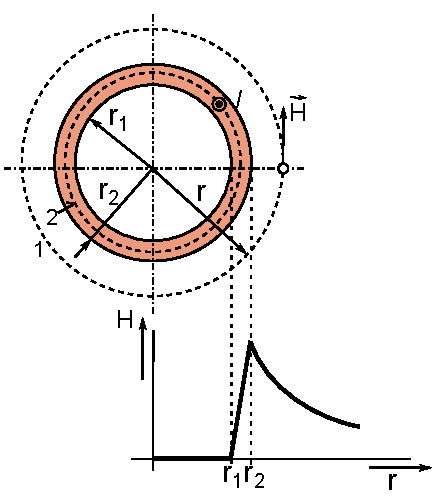
\includegraphics[width=0.8\linewidth]{teo_fig065.pdf}
      \captionof{figure}{K příkladu stanovení intenzity magnetického pole dlouhého dutého válcového 
                vodiče protékaného proudem}
      \label{teo:fig065}
    \par}
    
    Vodič s rovnoměrně rozloženým proudem podle obr. \ref{teo:fig065} je rotačně souměrný podle své
    osy a tedy i jeho magnetické pole je souměrné. Silové čáry jsou soustředné kružnice, vektor
    $\vr{H}$, jenž má směr tečny ke kružnici, je po celé délce kružnice stejně velký. Lze tedy
    snadno použít integrálního tvaru 1. MR (\textbf{zákon celkového proudu})
    
    Pro body ležící vně vodiče obepíná kruhová integrační dráha (vedená po silové čáře 1) celý
    proud vodiče $I$ a platí
    \begin{equation}\label{TEMP:eq_1MR_duty_valec}
      \oint_{\mathcal{C}}\vr{H}d\vr{l} = H\cdot 2\pi r = I
    \end{equation}
    takže intenzita pole je
    \begin{equation}\label{TEMP:eq_H_duty_valec}
      H = \frac{I}{2\pi r}
    \end{equation}
    
    Ve stěně dutého magnetického vodiče jsou silové čáry rovněž kružnice, neboť magnetické pole
    je i zde souměrné. Tyto siločáry však obepínají jen část proudu $I'$ vodiče pro oběh siločáry
    2 platí
    \begin{equation}\label{TEMP:eq_1MR_uvnitr_valce}
      \oint_{\mathcal{C}}\vr{H}d\vr{l} = H\cdot 2\pi r = I' = \pi(r^2-r_1^2)J
    \end{equation}
    kde $J$ je hustota proudu ve vodiči
    \begin{equation}\label{TEMP:eq_J_duty_valec}
      J = \frac{I}{S}= \frac{I}{\pi(r_2^2-r_1^2)}
    \end{equation}
    Ve stěně vodiče je tedy intenzita pole
    \begin{equation}\label{TEMP:eq_H_uvnitr_valce}
      H = \frac{I}{2\pi r}\frac{r^2-r_1^2}{r_2^2-r_1^2}
    \end{equation}
    V dutině vodiče je intenzita rovna nule. Vzhledem k souměrnosti pole by i zde muselo platit
    $\oint_{\mathcal{C}}\vr{H}d\vr{l} = H\cdot 2\pi r$. Protože dráha s poloměrem $r<r_1$ neobepíná
    žádný proud, je $\oint_{\mathcal{C}}\vr{H}d\vr{l} = 0$ a tedy musí byt $H = 0$.
  \end{example}    
\end{mdframed}  
      %------------------------------------------------------------------

      % --------example: $H=f(r)$ souosého kabelu -----------------------
      % \label{TEO:exam013}
      % !TeX spellcheck = cs_CZ
\begin{example}\label{TEMP:ex_koax_H}
  Stanovte intenzitu magnetického pole dlouhého přímého souosého kabelu podle obr.
  \ref{TEMP:fig_exam_koax}. Středním vodičem (\emph{žílou}) prochází proud $I$ a týž proud 
  opačného smyslu prochází vnějším vodičem (\emph{pláštěm}). Proudy jsou rovnoměrně rozloženy po 
  průřezech vodičů. Nakreslete graf průběhu $H = f(r)$ \cite[s.~92]{Dufek1970},
  \cite[s.~195]{Kotlan1999}.
  
  {\centering
   \begin{tabular}{cc}
     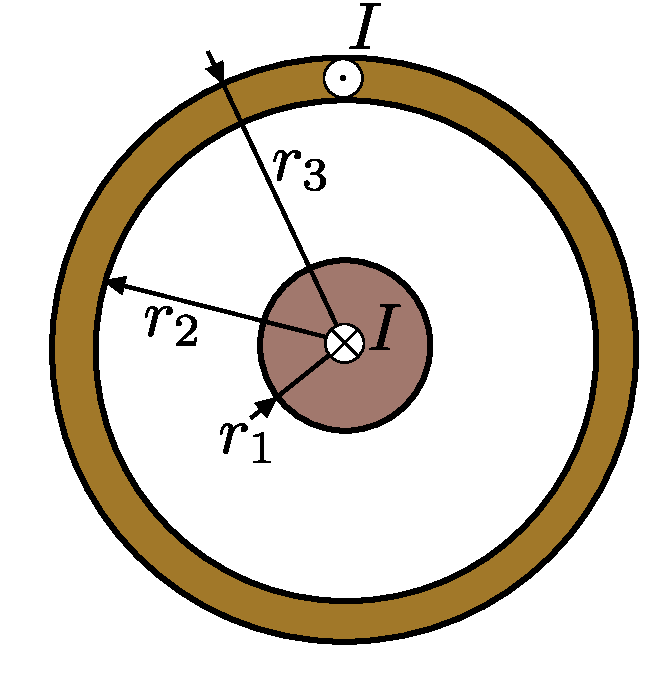
\includegraphics[width=0.4\linewidth]{vypocet_H_sousy_kabel.pdf}   &
     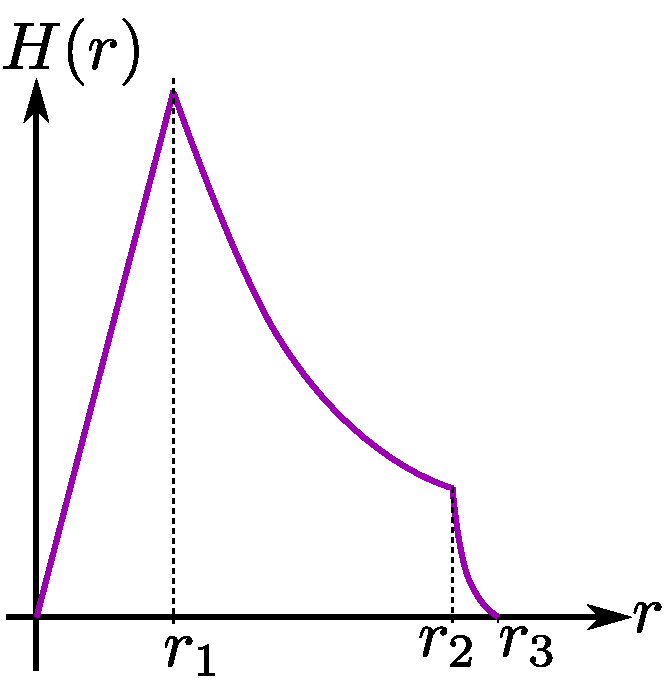
\includegraphics[width=0.4\linewidth]{koax_H_prubeh.pdf}
  \end{tabular}
  \captionsetup{type=figure}
  \captionof{figure}{K příkladu stanovení intenzity magnetického pole dlouhého souosého kabelu 
             protékaného proudem: a) náčrt; b) $H=f(r)$}
  \label{TEMP:fig_exam_koax}
  \par}
  
  \textbf{Řešení}: \newline Rovnici \ref{TEMP:eq_1MR_v_hom_p} aplikujeme na jednotlivé intervaly 
  osově souměrného stacionárního magnetického pole, přičemž se prakticky jedná o superpozici dvou
  polí. V oblasti $r<r_2$ se uplatňuje pouze pole vnitřního válcového vodiče (žíly), pro $r>r_2$ 
  přistupuje souosé pole vnějšího trubkového vodiče.
  \begin{itemize}
    \item Pro oblast $r<r_1$ je vzhledem k 
          \begin{align*}
              % \nonumber to remove numbering (before each equation)
              dI   &= \vr{J}d\vr{S} \\
              I(r) &= \int_S dI = \int_S \vr{J}d\vr{S} = \int_S J\cos\beta dS \\
                   &= \left|\begin{array}{cc}
                               \beta = 0 & H = \text{konst} \\
                             S = \pi r^2 & dS = 2\pi rdr \\
                            \end{array}
                      \right| = J\int_0^r 2\pi rdr = J\pi r^2
          \end{align*}
          hledané řešení 1. MR dáno 
          $$\oint_\mathcal{C}\vr{H}d\vr{l} = H_1 2\pi r = I(r) = J\pi r^2$$ kde celková proudová
          hustota je  $$J = \frac{I}{\pi r_1^2}$$ a tedy $$H_1 = \frac{I}{2\pi r_1^2}\cdot r$$
          
    \item Pro oblast $r_2>r>r_1$ řešíme v podstatě pole vně osamoceného válcového vodiče
          $I(r)$ a tedy $$H_2 = \frac{I}{2\pi r}$$
    \item Pro $r>r_3$ je magnetické pole vytvářeno celým proudem žíly $I$ a příslušnou částí
          proudu pláště $J\pi(r^2 - r_2^2)$, kde proudová hustota $$J =
          \frac{I}{\pi(r_3^2-r_2^2)}$$ má opačnou orientaci oproti proudové hustotě žíly. Pak 
          \begin{align*}
            I(r)                           &= I - I\frac{r^2-r_2^2}{r_3^2-r_2^2} \\
            \oint_\mathcal{C}\vr{H}d\vr{l} &= H_32\pi r = I(r)                   \\          
            H_3                            &= \frac{I}{2\pi r}\left(1 - 
            \frac{r^2 - r_2^2}{r_3^2 - r_2^2}\right) 
          \end{align*}
          Stejný výsledek dostaneme superpozicí opačně orientovaných polí $$H_3 = H'_3 - H''_3 =
          \frac{I}{2\pi r} - \frac{I}{2\pi r}\left(\frac{r^2 - r_2^2}{r_3^2 - r_2^2}\right)$$. 
  \end{itemize}
  Průběh $H(r)$ je na obr. \ref{TEMP:fig_exam_koax}.
\end{example}
  
      %------------------------------------------------------------------

    % -----------Magnetické pole elektrického proudu v diferenciálním tvaru-----------------------
    \subsection{Magnetické pole elektrického proudu v diferenciálním tvaru}
      Nechť je opět magnetické pole vyvoláno konstantním el. proudem $I = \text{konst}$. Jak
      vyplývá z předchozí kapitoly, základním vztahem pro toto pole je \emph{Ampérův zákon}
      $$\oint_{\mathcal{c}}\vec{H_c}\dd{\vec{l}} = I$$  Zvolme za integrační dráhu $c$ obvod malé plošky
      $\Delta S$, jíž prochází proud $\Delta I = J_n \Delta S$, kde $J_n$ je průmět vektoru hustoty
      proudu do směru normály plošky $\Delta S$ (předpokládáme, že ploška $\Delta S$ je dostatečně
      malá, aby se dalo počítat s konstantní hustotou proudu v celém jejím rozsahu)
      \cite[s.~13]{Trnka1972}. Pro zvolený případ platí
      
      \begin{equation}\label{TEMP:eq_amp_z1}
        \oint_{\mathcal{c}}\vec{H_c}\dd{\vec{l}}  =
          J_n \Delta S \rightarrow \frac{1}{\Delta S}\oint_{\mathcal{c}}\vec{H_c}\dd{\vec{l}} = J_n
      \end{equation} 
      
      Pro $\Delta S \rightarrow 0$ zavedeme označení 
      \begin{equation}\label{TEMP:eq_amp_z2}
        \rot{H}  = \frac{1}{\Delta S}\oint_{\mathcal{c}}\vec{H_c}\dd{\vec{l}}  = J_n
      \end{equation}
      
      Rovnice \ref{TEMP:eq_amp_z2} říká, že \emph{rotace vektoru} $\vec{H}$, ($\rot{H}$), jehož
      průmět do určitého směru je roven průmětu vektoru hustoty proudu do tohoto směřu. Z uvedených
      vztahu je patrný fyzikální význam rotace vektoru $\vec{H}$. Je to vektor, jehož velikost je
      rovna oběhovému magnetickému napětí po dráze v rovině kolmé k vektoru hustoty proudu,
      vztaženém k ploše obepínané oběhovou drahou (v nehomogenní poli to platí pro případ, že se
      plocha dráhy blíží k nule).
      
      Při použití pravoúhlé soustavy kartézských souřadnic \(x\), \(y\) a $z$ jsou průměty vektoru
      $\rot{H}$ do jednotlivých os
      \begin{equation}\label{TEMP:eq_amp_z3}
        \textsf{rot}_x\vec{H} = J_x,   \quad
        \textsf{rot}_y\vec{H} = J_y,   \quad
        \textsf{rot}_z\vec{H} = J_z    
      \end{equation}      
      Průmět $\textsf{rot}_x\vec{H}$ je dán oběhovým magnetickým napětím po obvodu plošky
      \(\dd{y}\dd{z}\) a platí
      \begin{align*}
        \textsf{rot}_x\vec{H} 
        &=\frac{1}{\dd{y}\dd{z}}\oint_{\mathcal{c}}\vec{H_c}\dd{\vec{l}} =               \nonumber\\
        &=\frac{1}{\dd{y}\dd{z}}\cdot\Biggl[\Biggr.\left[H_y\dd{y} 
         +\left(H_z + \pder{Hz}{y}\dd{y}\right)\dd{z}\right]                             \nonumber\\     
        &-\left[\left(H_y-\pder{H_y}{z}\dd{z}\right)\dd{y}-H_z\dd{z}\right]\Biggl.\Biggr]\nonumber\\
        &=\pder{H_z}{y}\dd{y}\dd{z} - \pder{H_y}{z}\dd{y}\dd{z}                          \nonumber\\    
        &=\pder{H_z}{y} - \pder{H_y}{z} = J_z
      \end{align*}       
      
      \luagraphic[0.8]{teo_fig062.pdf}{K odvození pojmu \(\textsf{rot}_z\vec{H}\)}{teo:fig062}
         
      tedy dostáváme
      \begin{subequations}
        \begin{align}\label{TEMP:eq_amp_z5}
          \textsf{rot}_x\vec{H} &= \pder{H_z}{y} - \pder{H_y}{z} = J_x       \\
          \textsf{rot}_y\vec{H} &= \pder{H_x}{z} - \pder{H_z}{x} = J_y       \\
          \textsf{rot}_z\vec{H} &= \pder{H_y}{x} - \pder{H_x}{y} = J_z            
        \end{align}    
    \end{subequations}    
      Pro \emph{pravoúhlé souřadnice} $x, y, z$ můžeme tedy vztah $\rot{H} = \vec{J}$ rozepsat na
      tvar
      \begin{align*}
        \textsf{rot}\vec{H} 
          &= \vec{i}\,\textsf{rot}_x\vec{H} + 
             \vec{j}\,\textsf{rot}_y\vec{H} +
             \vec{k}\,\textsf{rot}_z\vec{H}                                    \\
          &= \vec{i}\left(\pder{H_z}{y} - \pder{H_y}{z}\right) +               \\
          &+ \vec{j}\left(\pder{H_x}{z} - \pder{H_z}{x}\right) +               \\
          &+ \vec{k}\left(\pder{H_y}{x} - \pder{H_x}{y}\right)                 \\  
          &= \vec{i}\,J_x + \vec{j}\,J_y + \vec{k}\,J_z = \vec{J}.
      \end{align*}          
      
      Rotaci vektoru $\rot{H}$ můžeme též symbolicky vyjádřit vektorovým součinem Hamiltonova
      operátoru a vektoru $\vec{H}$
      \begin{align*}
        \rot{H} &= \nabla\times\vec{H}                                                      \\                                           
                &= \left(\vec{i}\,\pder{ }{x} + 
                   \vec{j}\,\pder{ }{y} + \vec{k}\,\pder{ }{z}\right)                       \\
                & \times(\vec{i}\,H_x + \vec{j}\,H_y + \vec{k}\,H_z)
      \end{align*}
      nebo také determinantu
      \begin{equation}\label{TEMP:eq_amp_z8}
        \rot{H} = \begin{vmatrix}
                    \vec{i}       & \vec{j}      & \vec{k}      \\
                    \pder{ }{x}  & \pder{ }{y} & \pder{ }{z} \\ 
                    H_x          & H_y         & H_z         \\
                  \end{vmatrix}      
      \end{equation}  
      \emph{cylindrických souřadnic} $r$, $\varphi$, $z$:
      \begin{align}\label{TEMP:eq_amp_z9}
        \textsf{rot}_r\vec{H}       
          &= \frac{1}{r}\pder{H_z}{\varphi} - \pder{H_\varphi}{z} = J_r           \nonumber \\ 
        \textsf{rot}_\varphi\vec{H} 
          &= \pder{H_r}{z} - \pder{H_z}{r}                        = J_\varphi     \nonumber \\
        \textsf{rot}_z\vec{H}       
          &= \frac{1}{r}\left[\pder{ }{r}
             \left(rH_\varphi\right)-\pder{H_r}{\varphi}\right]   = J_z
      \end{align} 
      \emph{sférických souřadnic} $r$, $\varphi$, $\vartheta$ 
      \begin{align}\label{TEMP:eq_amp_z10}
        \textsf{rot}_r\vec{H}        
           &= \frac{1}{r\sin\vartheta}\left[\pder{ }{\vartheta}(H_\varphi\sin\vartheta) - 
              \pder{H_\vartheta}{\varphi}\right]                     = J_r           \nonumber \\ 
        \textsf{rot}_\varphi\vec{H}   
           &= \frac{1}{r}\left[\pder{ }{r}(rH_\vartheta) - 
              \pder{H_r}{\vartheta}\right]                           = J_\varphi     \nonumber \\
        \textsf{rot}_\vartheta\vec{H} 
           &= \frac{1}{r\sin\vartheta}\left[\pder{H_r}{\varphi} -
              \pder{ }{r}\left(rH_\varphi\sin\vartheta\right)\right] = J_\vartheta    
    \end{align} 
      Podobně jako v elektrickém poli vyjadřujeme vztah $\oint\vec{D}\dd{\vec{S}} = Q$ vztahem 
      $\diver{D}
      = \rho$, tak i v magnetickém poli vyjadřujeme vztah $\oint\vec{B}\dd{\vec{S}} = 0$ vztahem
      $\diver{D} = 0$, nebo též v kartézských souřadnicích \(x\), \(y\) a $z$ jako $$\diver{D} =
      \nabla\cdot\vec{B} = \pder{B_x}{x} + \pder{B_y}{y} + \pder{B_z}{z} = 0$$
                     
    % ----------------Rovnice pro magnetický potenciál -------------------------------------------
    \subsection{Rovnice pro magnetický potenciál}
      V regulárních bodech lineárního homogenního izotropního magnetika platí pro $\varphi_m$
      \textbf{Laplaceova rovnice}
      \begin{equation}\label{TEMP:eq_varphi_m_laplace}
        \Delta\varphi_m = 0
      \end{equation}      
      Důkaz plyne z rovnice $\diver{B} = 0$ a rovnice $\vec{B} = \mu\vec{H}$: $$\diver{B} =
      \textsf{div}\mu\vec{H} = \textsf{div}\mu(-\textsf{grad}\varphi_m).$$ Pro $\mu = \text{konst}$
      dostáváme $\textsf{div}\textsf{grad}\varphi_m = 0$, což je rovnice
      \ref{TEMP:eq_varphi_m_laplace}.
      
      Na rozhraní mezi dvěma magneticky různými prostředími neplatí Maxwellovy rovnice v
      diferenciálním tvaru a tedy ani Laplaceova rovnice \ref{TEMP:eq_varphi_m_laplace}. Podmínky 
      pro $\vec{H}$ a $\vec{B}$ na rozhraní vyjádříme pomocí skalárního magnetického potenciálu
       \begin{align}\label{TEMP:eq_mag_U_rozhrani}
         \varphi_{m1}                 &= \varphi_{m2} \\
         \mu_1\pder{\varphi_{m1}}{n}  &= \mu_2\pder{\varphi_{m2}}{n} 
       \end{align}
      kde $\pder{}{n}$ jsou derivace ve směru normály k rozhraní. 
    
    \subsubsection{Vektorový magnetický potenciál}
      V elektrostatice jsme pro usnadnění mnohých problémů zavedli skalární elektrický potenciál -
      lze jej zavést vždy, neboť elektrostatické pole je vždy potenciální. Magnetické pole je však
      obecně vírové. Lze jej popsat skalárním potenciálem jen ve speciálních případech, tj.
      jestliže je polem potenciálním. Obecně je však zavedení skalárního potenciálu nepřípustné.
      Lze i pak zavést nějakou veličinu (analogickou skalárnímu potenciálu), s níž by se pracovalo
      snáze, než přímo s vektory pole?
      
      Dříve než definujeme vektorový magnetický potenciál, zopakujme zavedení skalárního potenciálu
      v elektrostatice. Vyjdeme z 2. MR a z rovnice známé z vektorové analýzy: $$\rot{E} = 0 \quad
      \text{a} \quad \textsf{rot}\,\textsf{grad}\varphi_m = 0.$$
      
      V magnetickém poli vyjdeme ze 4. MR a z jiné identity pro vektorovou funkci $\vec{A}$, známe z
      vektorové analýzy: $$\diver{B} = 0 \quad \text{a} \quad \textsf{div}\textsf{rot}\vec{A} =
      0$$ odtud
        \begin{equation}\label{TEMP:eq_B_rotA}
          \vec{B} = \rot{A}.
        \end{equation}       
               
%} % tikzset
%~~~~~~~~~~~~~~~~~~~~~~~~~~~~~~~~~~~~~~~~~~~~~~~~~~~~~~~~~~~~~~~~~~~~~~~~~~~~~~~~~~~~~~~~~~~~~~~~~~
  % % !TeX spellcheck = cs_CZ
% file: kap_zakld_zakn_elmag.tex
%{\tikzset{external/prefix={tikz/TEO/}}
% \tikzset{external/figure name/.add={ch02_}{}}
%====================Kapitola: Základní zákony elektromagnetismu====================================
\setchaptertoc
\chapter{Základní zákony elektromagnetismu}\label{teo:IchapII}
  V této teoreticky změřené kapitole budou shrnuty základní fyzikální zákony, kterými se řídí
  elektromagnetické jevy a jejichž znalost bude nezbytná při studiu následujících praktičtěji
  zaměřených kapitol. Mezi nejdůležitější patří zákon elektromagnetické indukce. Velký praktický
  význam má jeho zobecnění i pro případy nejsložitější, jakými jsou \emph{nelineární} a navíc
  \emph{parametrické} magnetické obvody. Důležitým pojmem je \emph{spřažený} magnetický tok cívky.
  Pro hlubší pochopení všech zákonitostí bude vhodné upozornit na \emph{topologické vlastnosti}
  elektromagnetického pole. Ukazuje se totiž, že topologický přístup je velice užitečným a silným
  nástrojem, který významně usnadňuje pochopení
  \href{http://en.wikipedia.org/wiki/Maxwell_theory}{Maxwellových rovnic} se všemi jejich důsledky
  \cite[s.~6]{Patocka4}. Topologii elektromagnetického pole je proto věnována celá kapitola
  \ref{teo:IchapIII}
  
  \section{Zákon elektromagnetické indukce}\label{teo:IchapIIsecI}
    Základní veličinou pro popis magnetických polí a jejich účinků je \emph{vektor magnetické
    indukce} \(\vec{B}\). Dle soustavy SI je jednotkou magnetické indukce \emph{tesla} \([T]\) a
    projevuje se silovými účinky na vodiče protékané proudy a indukováním napětí při jeho změně.

    Je proto dobře měřitelný. První rovnice (Ampérův zákon) ze souboru Maxwellových rovnic určuje
    rovnost oběhového integrálu magnetické indukce po uzavřené křivce proudům protékaných vodiči,
    jež jsou touto křivkou uzavřeny.
    \begin{equation}\label{es:eq_amp_law}
      \oint_l \vec{B} \cdot \vec{dl} = \sum I
    \end{equation}
    
    \luagraphic[0.6]{teo_fig034.pdf}{Elektrický proud ve vodiči způsobuje vznik magnetické pole v 
      jeho okolí.}{teo:fig034}

    Obrázek \ref{teo:fig034} ilustruje fakt, že elektrické proudy jsou vždy obklopeny 
    magnetickými poli. Tato pole se dají zesílit cívkou s magnetickým jádrem. Na tomto jevu je 
    založen jeden z elementárních principů elektrotechniky.    
       
    \begin{mdframed}[style=mdnote]
      Jaký je vztah jednotky magnetické indukce k ostatním základním jednotkám soustavy \textbf{SI}? 
      \begin{align*}
      1T &= 1\frac{V\cdot s}{m^2} = 1\frac{N}{A\cdot m} = 1\frac{Wb}{m^2}          \\
         &= 1\frac{kg}{C\cdot s} = 1\frac{kg}{A\cdot s^2} = 1\frac{N\cdot s}{C \cdot m}
      \end{align*}
    \end{mdframed}
    
    Při odvozování matematického modelu transformátoru se obvykle vychází ze zákona 
    \textbf{elektromagnetické indukce}, který říká, že \emph{časová změna magnetického pole vytvoří 
    vírové pole elektrické}:
    \begin{equation}\label{es:eq_ind_z}
      \oint_l \vec{E} \cdot \dd{\vec{l}} = - \der{\Psi}{t}
    \end{equation}
     
    Základní laboratorní experimenty, vedoucí k odhalení existence tohoto zákona, uskutečnil 
    \emph{Faraday}\footnote{Michael Faraday (1791 - 1867), samouk, zakladatel klasické 
    elektrodynamiky, vynikající experimentátor: Zavedl pojem fyzikálního prostorového pole pomocí 
    siločár, tzv. ''trubic''} r. 1831. Matematickou formulaci \emph{indukčního zákona} v podobě 
    rovnice
    \begin{equation}\label{ES:eq_zakl_elm25}
      u(t) = - \frac{d\Psi(t)}{\dd{t}}
    \end{equation} 
    stanovil již on sám, postupně význam zákona formálně upřesňovali další badatelé např.
    \emph{Neumann}\footnote{Franz Ernst Neumann (1798 - 1895), teoretický fyzik, matematik,
    mineralog. Definoval pojem magnetický vektorový potenciál, formuloval Neumannův vzorec pro
    vzájemnou indukčnost dvou smyček. Učitel G. R. Kirchhoffa.} kolem roku 1845. Konečné znění
    Maxwellovy teorie včetně formulace indukčního zákona do podoby II. Maxwellovy rovnice budoval
    Maxwell\footnote{James Clark Maxwell (1831 - 1879), teoretický fyzik, působil na Trinity College
    university v Cambridge, na King's College v Londýně, posléze první ředitel Cavendishovy
    laboratoře na univerzitě v Cambridge. Původně se zabýval teoretickou mechanikou a kinetickou
    teorií plynů. Soustavu čtyř Maxwellových rovnic odvodil především na základě
    mechanicko-elektrických analogií.} velmi pozvolna, v období 1855 až 1873. Z historického pohledu
    je zajímavé a důležité, že přesné \emph{kvantitativní} experimenty s elektromagnetickou indukcí
    byly v té době uskutečnitelné pouze pomocí
    \href{http://en.wikipedia.org/wiki/Galvanometer}{balistického galvanometru}. Lze odhadnout, že
    nebýt tohoto přístroje, přesná matematická formulace indukčního zákona by se pravděpodobně
    opozdila o několik let. Kupodivu, z psychologického hlediska je i v současnosti velmi vhodné
    vysvětlit princip indukčního zákona pomocí historických pokusů s balistickým galvanometrem.
    
    \subsection{Pokusy s balistickým galvanometrem}
      Jako každý elektromagnetický měnič energie (tj. motor), obsahuje i \emph{magnetoelektrické
      měřicí} ústrojí galvanometru dva akumulátory energie: moment setrvačnosti \(J\) otoč\-né 
      části a indukčnost cívky \(L\). Jedná se tedy o kmitavou soustavu 2. řádu. Každou takovou 
      soustavu lze kriticky, případně nadkriticky tlumit - především zařazením tlumicího odporu 
      vhodné velikosti do série s měřicím systémem (tlumení vlivem mechanického tření je úmyslně 
      konstrukčně potlačeno na zanedbatelnou úroveň). Balistický galvanometr je cíleně konstruován 
      s velkým momentem setrvačnosti \(J\) a s malou tuhostí \(k_d\) direkčních pružin, aby měl 
      dlouhou dobu kmitu \(T_G = 2\pi\sqrt{J/k_d}\) několik sekund. Proteče-li galvanometrem krátký 
      proudoý impuls \(i(t)\) o celkové délce \(t_i\) podle obr. \ref{teo:fig036}, pak lze snadno 
      dokázat, že za předpokladu \(t_i\ll T_G\) je první maximální výchylka \(\alpha_{max}\) 
      tlumeného pohybu ukazatele přímo úměrná celkovému náboji \(Q\) proudového impulsu podle 
      rovnice 
      \begin{equation}\label{ES:eq_zakl_elm01}
        \alpha_{max} = k_b Q = k_b\int_0^{t_i} i(t)\dd{t},
      \end{equation}
      kde \(k_b\) je \emph{balistická konstanta} použitého galvanometru. Balistický galvanometr tedy
      pracuje jako \emph{integrátor} proudu v přesném matematickém smyslu. 
      
      \luagraphic[1]{teo_fig036.pdf}{Příklad krátkého proudového impulsu prošlého balistickým 
        galvanometrem.}{teo:fig036}
  
      Uvažujme experiment uspořádaný podle obr. \ref{teo:fig037}. V uzavřeném obvodu
      galvanometru se nachází celkový odpor \(R\) a tuhá samonosná cívka v podobě kruhového závitu,
      připojená na dlouhé ohebné zkroucené přívody. Husté zkroucení zajišťuje, že do samotných
      přívodů se nemůže indukovat žádné napětí, pohybuje-li se cívka v magnetickém poli 
      permanentního magnetu. Při rychlém přesunu z polohy \emph{1} do vzdálené polohy \(\infty\) 
      klesne v cívce magnetický tok na nulu, časová změna toku zapříčiní vznik indukovaného napětí, 
      napětí protlačí obvodem proudový impuls odpovídající přibližně obr. \ref{teo:fig036}.
      
      \luagraphic[1]{teo_fig037.jpg}{Uspořádání experimentálního pracoviště s balistickým 
        galvanometrem}{teo:fig037}
      
      Za předpokladu kritického nebo nadkritického tlumení má odpor \(R\) relativně velkou hodnotu. 
      Proto lze s dobrou přesností zanedbat vnitřní indukčnost měřicího systému galvanoměru a 
      uvažovat, že celé napětí \(u(t)\), indukované v cívce při jejím pohybu, spočine pouze na 
      odporu. V uzavřeném okruhu o celkovém odporu \(R\) pak platí Ohmův zákon ve tvaru
      \begin{equation}\label{ES:eq_zakl_elm02}
        i(t)=\frac{u(t)}{R}.
      \end{equation}    
      Dosadíme-li rovnici \ref{ES:eq_zakl_elm02} do \ref{ES:eq_zakl_elm01}, po úpravě získáme vztah
      \begin{equation}\label{ES:eq_zakl_elm03}
       \int_0^{t_i}u(t)\dd{t}=\frac{\alpha_{max}R}{k_b}.
      \end{equation}     
      Experimentálně je možno dospět ke dvěma stěžejním poznatkům:
      \begin{itemize}
        \item Při přesunu cívky z polohy \emph{1} do polohy \(\infty\) nezávisí výchylka
              \(\alpha_{max}\) na \emph{rychlosti pohybu}. (Za předpokladu \(t_i\ll T_G\), což je
              omezení dané nedokonalostí přístroje a nijak nesouvisí se zkoumaným jevem.)
        \item Při přesunu cívky z polohy \emph{1} do polohy \(\infty\) zůstává součin
              (\(\alpha_{max}\times R\)) stále \emph{konstantní}, měníme-li úmyslně velikost odporu
              \(R\). To jest: při k-násobném zvýšení odporu klesne výchylka k-krát a naopak. 
      \end{itemize}
  
      V poloze „1“ prochází plochou cívky magnetický tok \(\Psi\). V poloze „\(\infty\)“ je zřejmě
      magnetický tok cívky nulový, tedy \(\Psi_\infty = 0\). S ohledem na rovnici
      (\ref{ES:eq_zakl_elm03}) lze pak oba experimentální poznatky interpretovat jediným možným
      způsobem:
       \begin{equation}\label{ES:eq_zakl_elm04}
       \int_0^{t_i}u(t)\dd{t}=\text{konst}=\Psi-\Psi_\infty=\Psi.
      \end{equation}    

      Experiment lze opakovat s cívkami libovolných rozměrů, tvarů i počtů závitů. Výsledky budou
      kvalitativně stejné. Veličina \(\Psi\) se nazývá \emph{spřažený magnetický tok cívky}. Je to 
      míra interakce cívky s magnetickým polem, které spojitě prostupuje celou plochou cívky. 
      Rovnici (\ref{ES:eq_zakl_elm04}) lze vyjádřit slovně: Spřažený magnetický tok cívky je úměrný 
      časovému integrálu svorkového napětí na zkoumané cívce. Je určitě výhodné zvolit jedničku 
      jako konstantu úměrnosti mezi tokem \(\Psi\) a integrálem napětí. \emph{Pak bude velikost 
      spřaženého toku přímo rovna integrálu napětí}. Určitý integrál v rovnici 
      (\ref{ES:eq_zakl_elm04}) lze nahradit integrálem neurčitým, pak je ale nutno přidat obecnou 
      počáteční integrační konstantu \(\Psi_0\)
      v newtonovském smyslu. Získáme tak zákon elektromagnetické indukce (indukční zákon) v
      integrálním tvaru
      \begin{equation}\label{ES:eq_zakl_elm05}
       \Psi(t) = \Psi_0 + \int u(t)\dd{t} \quad [Wb;\, V,\; s].
      \end{equation}   
    
    Z rovnice (\ref{ES:eq_zakl_elm05}) plyne, že jednotka magnetického toku Weber\footnote{Wilhelm
    Eduard Weber (1804-1891), teoretický fyzik, působil na univerzitách v Gottingenu a v Lipsku.
    Zakladatel předrelativistické elektrodynamiky. Určil totiž silu mezi náboji v závislosti nejen
    na vzdálenosti, ale i na rychlosti a zrychlení, jeho teorie je ale platná pouze pro \(v \ll c\).
    Blízký spolupracovník Gausse.} má rozměr \([Vs]\), Budeme-li obě strany rovnice derivovat podle
    času, rovnost tím neporušíme. Získáme tak ryze matematickou cestou indukční zákon v
    diferenciálním tvaru
    \begin{equation}\label{ES:eq_zakl_elm06}
     u(t) = \frac{d\Psi(t)}{\dd{t}}, \quad \text{resp.} \quad  u(t) = -\frac{d\Psi(t)}{\dd{t}}.
    \end{equation}   
    Obě rovnice (\ref{ES:eq_zakl_elm06}a), (\ref{ES:eq_zakl_elm06}b) se liší znaménkem \(+\) nebo
    \(-\) na pravé straně. Volba znaménka souvisí s domluvou, který režim cívky považujeme za
    základní: zda režim \emph{spotřebičový} podle rovnice (\ref{ES:eq_zakl_elm06}a), nebo režim
    \emph{zdrojový} podle rovnice (\ref{ES:eq_zakl_elm06}b). Oba režimy jakéhokoli dvojpólu jsou
    totiž jednoznačně definovány vzájemnou orientací napětí a proudu podle obr.
    \ref{teo:fig039}. Odpor nemůže nikdy pracovat jako zdroj, proto slouží jako
    „normál“ definující \emph{spotřebičovou} orientaci svorkových veličin. Oba režimy cívky se liší
    níže popsaným způsobem.

    \begin{figure}[ht!]
      \centering  
      \subcaptionbox{Odpor je vždy spotřebičem \label{teo:fig039a}    }{\luafigure[0.4]{teo_fig039a.pdf}}                    
      \subcaptionbox{Cívka ve spotřebičovém režimu \label{teo:fig039b}}{\luafigure[0.4]{teo_fig039b.pdf}}  
      \newline               
      \subcaptionbox{Cívka ve zdrojovém režimu \label{teo:fig039c}    }{\luafigure[0.4]{teo_fig039c.pdf}}
      \caption{Vzájemná orientace okamžité hodnoty proudu a napětí ve spotřebičovém a zdrojovém 
               režimu:} 
      \label{teo:fig039}
    \end{figure}
        
    \textbf{Spotřebičový režim:}
    \begin{itemize}[noitemsep]
      \item Orientace svorkového napětí \(u(t)\) je vůči proudu \(i(t)\) souhlasná. Platí rovnice
            (\ref{ES:eq_zakl_elm06}a).
      \item Cívka je připojena na zdroj napětí\(u(t)\), odebírá z něj proud \(i(t)\), tedy odebírá
            ze zdroje elektrickou energii a chová se jako spotřebič. Tuto energii přeměňuje na
            energii magnetického pole.
      \item Mezi směrem proudu a směrem toku platí \emph{pravidlo pravé ruky}, PPR.           
    \end{itemize}
    
    \textbf{Zdrojový režim:}
    \begin{itemize}[noitemsep]
      \item Orientace svorkového napětí u(t) je vůči proudu i(t) nesouhlasná. Platí rovnice
            (\ref{ES:eq_zakl_elm06}b).
      \item Cívka je vložena do proměnného magnetického pole \(B(t)\), na jejích svorkách vzniká
            indukované napětí \(u(t)\) (zastaralý výraz: „elektromotorická síla“). Z cívky se stal
            zdroj elektrického napětí u(t), tj. generátor. Připojíme-li na svorky odporovou zátěž,
            začne do ní generátor dodávat elektrickou energii.\footnote{Faraday s Maxwellem se
            znali osobně a po dohodě pokládali zdrojový režim cívky za základní, tedy pracovali s
            rovnicí (\ref{ES:eq_zakl_elm06}b). Maxwell navíc pracoval s pojmem „electromotive force
            \(P\)‘, který svým významem přesně odpovídal dnešní „intenzitě elektrického pole.
            Postupem času byl doslovně přeloženému výrazu „elektromotorická síla“ nešťastně
            přiřazen v české i zahraniční literatuře význam „napětí“, což ještě více zvýšilo
            zmatek. Proto je rozumné výraz „elektromotorická síla“ vůbec nepoužívat.}
    \end{itemize}

    \luagraphic[1]{teo_fig038.jpg}{Princip transformátoru. Primární cívka pracuje ve
    spotřebičovém režimu (PPR), sekundární cívka ve zdrojovém režimu (PLR)}{teo:fig038}

    Z uvedených skutečností lze učinit následující závěr. Volba znaménka v rovnicích
    (\ref{ES:eq_zakl_elm06}a, b) je věcí dohody, ale pouze v tom smyslu, zda zvolíme za základní
    režim spotřebičový či zdrojový\footnote{Ojediněle se v literatuře, např. v [5], vyskytne názor,
    že znaménko v rovnicích (\ref{ES:eq_zakl_elm06}a, b) je určeno tím, zda je cívka navinuta
    pravotočivě nebo levotočivé. To je chybné tvrzení. Pravotočivost či levotočivost cívky naprosto
    nijak nesouvisí se schopnosti cívky pracovat ve zdrojovém nebo spotřebičovém režimu.}. 
    Například při analýze měničů ve výkonové elektronice je ustáleným zvykem zvolit označení proudu
    a napětí na indukčnosti podle obr. \ref{teo:fig039b}. Bez ohledu na tuto volbu musíme v 
    konkrétní situaci vždy pečlivě rozlišovat, ve kterém režimu se cívka skutečně nachází.
    Příklad: primární cívka transformátoru se nachází vždy ve spotřebičovém režimu, sekundární
    cívka vždy ve zdrojovém režimu. Se zdrojovým či spotřebičovým režimem úzce souvisí \emph{Lenzův
    princip}\footnote{Heinrich Lenz (1804-1865), estonský fyzik, působil na univerzitě v
    Petrohradu. Princip po něm pojmenovaný objevil r. 1833.}. Jedná se o zvláštní případ
    obecnějšího přírodního principu, vyjádřitelného jako „zákon akce a reakce“. V elektromagnetismu
    má zákon následující tvar:

    Lenzův princip: Proud indukovaný v uzavřené vodivé smyčce vyvolá magnetické pole, které působí
    vždy proti původnímu budicímu poli, díky němuž indukovaný proud vznikl.

    Všimněme si, že zmíněná „uzavřená vodivá smyčka“ se nachází \emph{zdrojovém režimu}: je vložena
    do magnetického pole, indukuje se v ní napětí \(u(t)\), které protlačí vodivým obvodem proud
    \(i(t)\). Proud má ve \emph{zdrojovém režimu} takový směr, že působí proti budicímu magnetickému
    poli. Příkladem je již zmíněná sekundární cívka transformátoru podle Obr. /./-*/« nebo uzavřená
    smyčka vířivého proudu ve vnitřním prostoru transformátorového plechu podle Obr. 1.1-5.

    \luagraphic[1]{teo_fig040.jpg}{Vznik vířivého proudu uvnitř elektricky vodivého
    transformátorového plechu. Budicí cívka pracuje ve spotřebičovém režimu (PPR). Elementární
    smyčka vířivého proudu odpovídá sekundárnímu vinutí a pracuje ve zdrojovém režimu
    (PLR).}{teo:fig040}

    Integrací rovnice (\ref{ES:eq_zakl_elm06}a) lze zpětně dojít k integrálnímu tvaru
    (\ref{ES:eq_zakl_elm05}). Je nutno zdůraznit, že obě rovnice jsou naprosto rovnocenné, navzájem
    převoditelné, obě nesou stejné množství informace, žádná není důležitější než druhá. Je
    pravdou, že z psychologického pohledu je indukční zákon snáze pochopitelný v
    \emph{diferenciálním} tvaru (\ref{ES:eq_zakl_elm06}). Pro hluboké porozumění magnetickým jevům
    je však nezbytné uvědomit si především jeho \emph{integrální} podobu (\ref{ES:eq_zakl_elm05})
    se všemi matematickými důsledky:
    \begin{itemize}
      \item Spřažený tok je roven integrálu napětí. Zákon platí \emph{univerzálně}, bez ohledu na
            \emph{linearitu} či \emph{nelinearitu} magnetického obvodu. Rovnice
            (\ref{ES:eq_zakl_elm05}) totiž definuje funkční závislost \(\Psi=\Psi(u)\) mezi tokem a
            napětím, nikoli závislost \(\Psi=\Psi(i)\) mezi \emph{tokem a proudem}.  Případná
            nelinearita se totiž týká výlučně závislosti \(\Psi=\Psi(i)\), a tudíž nijak nenarušuje
            platnost rovnice (\ref{ES:eq_zakl_elm05}).
      \item Z předchozího bodu plyne, že v obecném \emph{nelineárním} případě není tok \(\Psi\)
            přímo úměrný proudu \(i\). Přímá úměra \(\Psi = Li\) totiž platí pouze ve zvláštním
            případě \emph{lineárního} magnetického obvodu.
      \item Rovnice (\ref{ES:eq_zakl_elm05}) platí ve spotřebičovém i generátorovém režimu cívky.
            Problém se znaménkem zůstává stejný jako u rovnic (\ref{ES:eq_zakl_elm06}).
      \item V uzavřené \emph{supravodivé} smyčce platí vždy \(u = 0\), i když jí teče konstantní
            ss. proud. Neurčitý integrál v rovnici (\ref{ES:eq_zakl_elm05}) má pak nulovou hodnotu
            \(\int0\dd{t}=0\), a zřejmě tedy platí \(\Psi(t)=\Psi_0\), kde \(\Psi_0\) je
            \emph{libovolná} počáteční integrační konstanta. Fyzikálně má konstanta význam
            počátečního toku, který je v cívce naintegrován z předchozích dějů. Případ
            \(\Psi_0\neq0\) odpovídá nabuzenému supravodivému magnetu, jehož tok \(\Psi(t)=\Psi_0
            = \text{konst.}\) se s časem nemění. Nabuzený supravodivý magnet se proto chová jako
            \emph{permanentní} magnet. Případ \(\Psi_0 = 0\) odpovídá magnetickému stínění pomocí
            \emph{závitu nakrátko}, např. tzv. Faradayova klec, nebo stínění koaxiálního kabelu
            podle obr. \ref{teo:fig041}. Každé oko \textbf{a-b-c-d} stínícího pláště
            tvoří „supravodivý“ závit nakrátko, v němž platí \(u = 0\), tedy \(\Psi=\int0\dd{t}=0\).
            Proto se do vnitřního prostoru ohraničeného pláštěm nemůže zvenčí dostat žádné
            \emph{střídavé} rušivé magnetické pole (jedině pole \emph{stejnosměrné} \(\Psi_{ss}\),
            ale to je neškodné, protože nezpůsobuje vznik rušivého napětí ve středním vodiči
            kabelu; derivace konstanty je totiž nulová: \(u(t)=\frac{d\Psi_{ss}}{\dd{t}}=0\)).
    \end{itemize}

    Na otázku „Proč je magnetický tok úměrný integrálu napětí?“ lze odpovědět pouze následujícím
    způsobem: „Protože je to jeden ze základních zákonů přírody, jehož správnost se nepodařilo
    experimentálně nikdy vyvrátit, nýbrž vždy pouze potvrdit.“ Deduktivní odvození indukčního
    zákona z vyšších přírodních zákonitostí není na úrovni klasické fyziky možné, není
    uskutečnitelné ani na vyšší úrovni \emph{kvantové elektrodynamiky}\footnote{Za objev kvantové
    elektrodynamiky obdržel Richard P. Feynman (1918-1988) Nobelovu cenu v r. 1965 (Feynmanovy
    fázorové diagramy a Feynmanův dráhový integrál; nositelé elektromagnetických sil jsou fotony). 
    Vynikající teoretický fyzik, ale i praktik. Celoživotně působil na kalifornském technickém
    institutu. Během druhé světové války byl členem týmu pracujícího na vývoji americké atomové
    bomby v Los Alamos (projekt Manhattan).}. Za povšimnutí stojí, že v diferenciální formě
    (\ref{ES:eq_zakl_elm06}) nebylo přesné kvantitativní ověření indukčního zákona v době objevu
    proveditelné s ohledem na možnosti tehdejšího přístrojového vybavení. Experiment v nehomogenním
    poli podle obr. \ref{teo:fig037} by byl i v současnosti velmi těžko   
    vyhodnotitelný. Naopak, ověření v integrálním tvaru je velmi snadné\footnote{V současnosti by
    byl balistický galvanometr nahrazen operačním zesilovačem zapojeným jako integrační zesilovač.
    Ten by zpracovával signál ze snímače proudu, např. z proudového bočníku. Po odeznění proudového
    impulsu by na výstupu zesilovače zůstalo naintegrováno určité konstantní napětí, jehož velikost
    by analogicky odpovídala maximální výchylce \(\alpha_{max}\) galvanometru.} . To opravňuje k
    domněnce vyslovené v historickém úvodu kapitoly.

    \begin{figure}[ht!]
      \centering  
      \subcaptionbox{\label{teo:fig041a}}{\luafigure[0.4]{teo_fig041a.jpg}}                    
      \subcaptionbox{\label{teo:fig041b}}{\luafigure[0.4]{teo_fig041b.jpg}}  
      \caption{Plášť koaxiálního kabelu. Každé oko \textbf{a-b-c-d} tvoří závit nakrátko.} 
      \label{teo:fig041}
    \end{figure}
      
    Supravodivá cívka podle obr. \ref{teo:fig042} začne být v okamžiku \(t = 0\)
    napájena ideálním zdrojem napětí \(u(t)\). Později na ni začne působit vnější magnetické pole
    přibližujícího se permanentního magnetu. Jaký vliv bude mít PM na velikost spřaženého toku
    cívky?
    
    Odpověď plyne přímo z rovnice (\ref{ES:eq_zakl_elm05}): \(\Psi(t) = \Psi_0 +\int u(t)\dd{t}\).
    
    Ze zadání příkladu vyplývá, že počáteční integrační konstanta je nulová. Neurčitý integrál je
    možno nahradit integrálem určitým. Velikost spřaženého toku je \emph{tvrdě definována}
    přiloženým napětím, tedy hodnotou určitého integrálu. Proto externí magnetické pole 
    \emph{nemůže} spřažený tok cívky nijak změnit. Ideální napěťový zdroj má \emph{nulový} 
    vnitřní odpor. Proto se supravodivá cívka napájená tímto zdrojem stále chová jako supravodivý
    závit nakrátko, do něhož nemůže vniknout žádná siločára externího magnetického pole.
    
    \begin{figure}[ht!]
      \centering  
      \subcaptionbox{\label{teo:fig042a}}{\luafigure[0.41]{teo_fig042a.jpg}}                    
      \hspace{1em}
      \subcaptionbox{\label{teo:fig042b}}{\luafigure[0.45]{teo_fig042b.jpg}}  
      \newline               
      \subcaptionbox{\label{teo:fig042c}}{\luafigure[0.41]{teo_fig042c.jpg}}
      \caption{K příkladu, a) Supravodivá cívka je napájená ideálním napěťovým zdrojem, b) Později
               na ni začne působit externí pole pohybujícího se magnetu, c) Náhradní zapojení.} 
      \label{teo:fig042}
    \end{figure}
  
    Jev lze vysvětlit následovně. Pohybující se magnet indukuje v cívce přídavné indukované napětí
    \(u(t)\). Toto napětí se přičte k napětí napájecímu a způsobí změnu proudu \(\Delta i(t)\)
    tekoucího cívkou. Podle Lenzova principu začne tento přídavný proud působit proti poli PM.
    Přídavný proud \(\Delta i(t)\) má přesně takovou velikost a směr, že uvnitř závitu dokonale
    vykompenzuje a zruší externí pole magnetu. Vnější pozorovatel tedy vidí, že supravodivý závit se
    chová jako magnetický izolant, jemuž se siločáry externího pole vyhnou, a celkový tok cívky není
    přítomností magnetu nijak ovlivněn. Celá soustava se navíc chová jako elektromechanický měnič
    energie (tj. motor), který je schopen pracovat v motorovém nebo generátorovém režimu. Pohybující
    se magnet totiž koná nebo spotřebovává mechanickou práci, protože na něj působí síla. Podle
    vzájemné okamžité orientace vektorů \emph{síly} a \emph{rychlosti} pracuje celá soustava buď
    jako motor (koná mechanickou práci), nebo jako generátor (spotřebovává mechanickou energii a
    ukládá ji do zdroje napětí).

    %------------- Spřažený tok vzduchové cívky ----------------------------------------------------
    \section{Spřažený tok vzduchové cívky}\label{ES:sec02}
      Experiment s galvanometrem popsaný v předchozí kapitole lze uskutečnit podrobněji ve čtyřech
      následujících modifikacích označených čísly \textbf{1} až \textbf{4}. Pro vyšší přehlednost
      budou těmito čísly systematicky značeny i veličiny v jednotlivých pokusech. Ze čtyř postupně
      gradujících experimentů vyplyne geometrická interpretace pojmu \emph{spřažený tok} vzduchové
      cívky. Poznámka: V následujících experimentech se pokusná  cívka nachází v generátorovém
      režimu. Učiníme však dohodu, že velikost toku budeme pro jednoduchost uvažovat v absolutní
      hodnotě, tj. bez ohledu na znaménko \cite[s.~12]{Patocka4}.

      \subsection{Experiment č. 1}
        Podle Obr \ref{teo:fig043} je na ohebných zkroucených přívodech umístěna tuhá samonosná
        cívka, která má jeden závit o ploše \(\Delta S\). Plocha musí být \emph{malá}, aby bylo
        možno předpokládat, že magnetické pole v těsném okolí cívky je \emph{homogenní} (vektor
        indukce \(\vec{B_1}\), musí být v rámci cívky konstantní). Malé rovinné ploše závitu je pak
        možno přiřadit vektor \(\Delta\vec{S_1}\), jehož směr je kolmý na onu rovinu. Opakováním
        pokusu při různých úhlech \(\alpha_1\), různě velkých plochách a různě velké indukci lze
        snadno zjistit, že velikost toku je přímo úměrná:

        \luagraphic[0.7]{teo_fig043.png}{Cívka má jeden závit o ploše \(\Delta S\). Výsledný vektor 
        plochy má proto velikost \(\Delta S_1 = 1\cdot\Delta S\). \cite[s.~13]{Patocka4}}{teo:fig043}

        \begin{itemize}[noitemsep]
          \item veličině \(\cos\alpha_1\),
          \item ploše závitu \(\Delta S_1 \equiv \Delta S\),
          \item magnetické indukce \(B_1\).
        \end{itemize}
        To vede k jednoznačnému závěru, že tok lze vyjádřit jako skalární součin vektoru plochy a
        vektoru mg. indukce v daném místě „l“:
        \begin{equation}\label{ES:eq_zakl_elm07}
          \int_0^{t_i} u(t)\dd{t} = \Psi_1 = B_1\Delta S_1\cos\alpha_1 = \vec{B_1}\cdot\Delta\vec{S_1}.
        \end{equation}  
     
      \subsection{Experiment č. 2}
        Vše zůstává stejné jako v předchozím experimentu. Na obr. \ref{teo:fig044} pouze vzrostl
        počet závitů cívky z jednoho na dva. Závity jsou umístěny těsně na sobě, proto máji stejnou
        plochu \(\Delta S\). Plochy se sčítají, proto má výsledný vektor \(\Delta \vec{S_2}\),
        velikost \(\Delta S_2\equiv2\Delta S\). Experiment ukazuje, že tok lze opět vyjádřit jako
        skalární součin vektoru plochy a vektoru magnetické indukce v místě „2“:

        \luagraphic[0.7]{teo_fig044.png}{Cívka má dva závity o ploše \(\Delta S\). Výsledný vektor
        plochy má proto velikost \(\Delta S_2 = 2\cdot\Delta S\).
        \cite[s.~13]{Patocka4}}{teo:fig044}
        
        \begin{align}
          \int_0^{t_i} u(t)\dd{t} = \Psi_2 
             &= B_2(2\Delta S)\cos\alpha_2                           \nonumber \\
             &= B_2(\Delta S_2)\cos\alpha_2 
              = \vec{B_2}\cdot\Delta\vec{S_2}.                       \label{ES:eq_zakl_elm08}
        \end{align}

      \subsection{Experiment č. 3}
        Na obr. \ref{teo:fig045} má cívka opět dva závity (počet závitů musí byt 
        přirozeným číslem). První závit má původní velikost \(\Delta S\), druhý závit má plochu 
        poloviční. Výsledný vektor \(\Delta S_3\), má tedy velikost \(\Delta S_3 = 
        \num{1.5}\cdot\Delta S\). Experiment ukazuje, že tok lze opět vyjádřit jako skalární součin 
        vektoru plochy a vektoru magnetické indukce v daném miste „3“:

        \luagraphic[0.7]{teo_fig045.png}{Cívka má dva závity první o ploše \(\Delta S\), druhý o
        ploše \(0,5\Delta S\). Výsledný vektor plochy má proto velikost \(\Delta S_1 =
        \num{1.5}\cdot\Delta S\). \cite[s.~13]{Patocka4}}{teo:fig045}

         \begin{align}
           \int_0^{t_i} u(t)\dd{t} = \Psi_3 
             &= B_3(\num{1.5}\Delta S)\cos\alpha_3                  \nonumber  \\
             &= B_3(\Delta S_3)\cos\alpha_3 
              = \vec{B_3}\cdot\Delta\vec{S_3}.                      \label{ES:eq_zakl_elm09}
         \end{align}
         
         Zdůrazněme, že číselný koeficient „\num{1.5}“ v rovnici (\ref{ES:eq_zakl_elm09}) 
         \textbf{nelze} interpretovat ve smyslu, že cívka má \num{1.5} závitů. Z topologického 
         hlediska není možné, aby počet závitů byl necelým číslem. Počet závitů musí být číslem 
         přirozeným, tj. 1, 2, 3, ... Nepřípustná je i nula: každý uzavřený obvod, kterým teče 
         proud, je totiž nutno topologicky interpretovat jako nejméně jeden závit. Koeficient 
         „\num{1.5}“ je proto nutno bezpodmínečně chápat jako velikost plochy, nikoli jako počet 
         závitů. Totéž platí o koeficientu „2“ v experimentu č. 2. Toto je klíčová topologická 
         úvaha, bez níž nelze pochopit geometrický význam pojmu spřažený tok cívky.
       
      \subsection{Experiment č. 4}
        Tento experiment je syntézou všech tři předchozích pokusů. Výsledná cívka na obr. 
        \ref{teo:fig046} je tvořena \emph{třemi dílčími cívkami}, přesně stejnými 
        jako v předchozích případech. Cívky tvoří tuhou samonosnou soustavu, navzájem jsou 
        nepohyblivé. Při pokusu se pohybují současně jako jediné těleso. Výchozí polohy „1“, „2“, 
        „3“ všech tří dílčích cívek jsou stejné jako dříve. Experiment pak ukazuje, že výsledný 
        tok je součtem toků ze všech tří předchozích pokusů:

        \luagraphic[0.7]{teo_fig046.png}{Výsledná cívka je tvořena třemi dílčími cívkami, přesně
        stejnými jako v předchozích případech. Cívky tvoří tuhou soustavu, která se pohybuje jako
        celek. \cite[s.~14l]{Patocka4}}{teo:fig046}

        \begin{align}
          \int_0^{t_i} u(t)\dd{t} = \Psi 
            &= \Psi_1 + \Psi_2 +\Psi_3                         \nonumber \\
            &= \vec{B_1}\cdot\Delta\vec{S_1} 
             + \vec{B_2}\cdot\Delta\vec{S_2} +
               \vec{B_3}\cdot\Delta\vec{S_3}.                  \label{ES:eq_zakl_elm10}
        \end{align}
        Experiment č. 4 je možno dále libovolně komplikovat, přidávat další dílčí cívky, měnit 
        jejich tvary, velikosti i počty závitů. Pro \(n\) dílčích cívek lze rovnici 
        (\ref{ES:eq_zakl_elm10}) psát v obecnějším tvaru:
        \begin{equation}\label{ES:eq_zakl_elm11}
          \Psi = \sum_{i=1}^n\vec{B_i}\cdot\Delta\vec{S_i}.
        \end{equation}

      \subsection{Vzduchová cívka ve tvaru šroubovice}
        Uvažujme však případ ještě složitější, jakým je vzduchová cívka ve tvaru šroubovice podle 
        obr. \ref{teo:fig047}. Nechť je cívka opět samonosná, navinutá z tuhého 
        vodiče zachovávajícího svůj pevný tvar. Z topologického pohledu má vodič význam hraniční 
        křivky \(l\), která tvoří hranici orientované plochy \(S\). Tvar plochy si lze představit 
        například těmito dvěma různými způsoby:

        \luagraphic[0.8]{teo_fig047.png}{Vzduchová cívka o čtyřech závitech. Celková plocha \(S\)
        cívky má tvar „čtyřzávitové šroubovice“. Vodič tvoří hraniční křivku \(l\) celkové plochy
        \(S\). \cite[s.~15]{Patocka4}}{teo:fig047}

        \begin{itemize}[noitemsep]
          \item Šroubovice, přibližně v tom smyslu jako šnek v mlýnku na maso nebo jako točité 
                schodiště.          
          \item Mýdlová membrána napnutá na vodič, pokud bychom vodič namočili a vzápětí vytáhli
                z mýdlového roztoku, podobně jako bublifuk.
        \end{itemize}
        Z topologického pohledu má plocha \(S\) dvě základní vlastnosti:
        \begin{itemize}[noitemsep]
          \item \textbf{ohraničená} - po obvodu je ohraničena nepřerušenou hraniční křivkou \(l\).
          \item \textbf{orientovaná} - má dvě izolované strany, které lze natřít dvěma různými 
                barvami, aniž se barvy potkají jinde než na protilehlých stranách hraniční křivky 
                \(l\).
        \end{itemize}
         
        Na obr. \ref{teo:fig047} je naznačeno, že všechny siločáry \(B\) nemusí procházet všemi
        čtyřmi závity. Pojem \emph{„průchod siločáry i-tým závitem“} je nutno chápat tak, že
        siločára protíná šroubovicovou plochu \(S\) v \emph{„i-tém poschodí šroubovice“}. Body
        protnutí jsou zdůrazněny tečkami. V horním závitu je naznačena diferenciální ploška \(dS)\),
        jejíž vektor \(\vec{dS}\) svírá s vektorem magnetické indukce \(\vec{B}\) úhel \(\alpha\).
        Při výpočtu celkového toku procházejícího cívkou (tedy celkovou plochou \(S\)) je nutno
        postupovat přesně podle rovnice (\ref{ES:eq_zakl_elm11}), tj.:
        \begin{itemize}[noitemsep]
          \item Plochu rozdělit na velké množství co nejmenších plošek \(\Delta\vec{S}\).
          \item Ve všech ploškách spočítat skalární součiny \(\vec{B}\cdot\Delta\vec{S}\).
          \item Skalární součiny sečíst.
        \end{itemize}
        
        Při neustálém zjemňování plošek přejde rovnice (\ref{ES:eq_zakl_elm11}) v limitním případě 
        do integrální podoby
        \begin{equation}\label{ES:eq_zakl_elm12}
          \Psi = \sum_{i=1}^n\vec{B_i}\cdot\Delta\vec{S_i} \qquad\Longrightarrow\qquad
          \Psi = \int_S\vec{B}\cdot \dd{\vec{S}}
        \end{equation}
        Integrál je nutno chápat jako \emph{plošný integrál} přes celou plochu \(S\). Uvnitř 
        integrálu musí figurovat \emph{skalární součin}, protože tok je skalár. Veličina \(\Psi\) 
        se nazývá \emph{spřažený tok} cívky. Je to celkový tok \emph{procházející} plochou \(S\) 
        neboli celkový tok \emph{interagující} s plochou \(S\). Zdůrazněme tyto skutečnosti:
        \begin{itemize}[noitemsep]
          \item Ve výpočtu nijak nefiguruje počet závitů \(N\), protože je již nepřímo obsažen v 
                podobě jednotlivých interakcí: protne-li některá siločára plochu k-krát, započte se 
                automaticky k interakcí.
        
          \item Plocha je orientovaná (má např. červenou a zelenou stranu). To znamená, že záleží 
                na směru protnutí, na \emph{směru} interakcí. Pak např. všechny interakce ve směru 
                \textbf{č} \(\rightarrow\) \textbf{z} jsou po dohodě \emph{kladné}, interakce 
                ve směru \textbf{z} \(\rightarrow\) \textbf{č} jsou \emph{záporné}.
        
          \item Cívka může mít podobu libovolně zdeformovaného vodiče. Pak bude velmi složitě 
                deformovaná i plocha \(S\). Plocha může libovolně protínat sama sebe a navinout se 
                libovolně několikrát na deformovaný vodič, viz kap. 2. Přesto bude rovnice 
                (\ref{ES:eq_zakl_elm12}) stále platná.
      \end{itemize}
      
      Je zřejmé, že ve složitých deformovaných případech nebude integrál (\ref{ES:eq_zakl_elm12}) 
      řešitelný v uzavřeném tvaru. To nevadí, smyslem těchto úvah totiž není řešení integrálu, 
      nýbrž pochopení jeho geometrického významu. Poznamenejme, že integrál je vždy možno vyřešit 
      numericky, pomocí rovnice (\ref{ES:eq_zakl_elm11}). Pouze je třeba rozdělit plochu na 
      dostatečně malé plošné elementy. Rovnici (\ref{ES:eq_zakl_elm11}) je tedy možno chápat jako 
      jeden ze základních návodů na řešení pole \emph{metodou konečných prvků}. Situace při výpočtu 
      integrálu (\ref{ES:eq_zakl_elm12}) však není tak beznadějná, jak se na první pohled zdá. Je 
      to dáno tím, že integrál má následující vynikající vlastnost, která bohužel obvykle nebývá v 
      literatuře zdůrazňována, a kterou lze vyslovit v podobě matematické věty:
      \begin{lemma}\label{es:fig_patocka_lemma01}
        Velikost plošného integrálu \(\Psi = \int_S\vec{B}\cdot\Delta \vec{S}\) přes plochu \(S\) 
        je \textbf{nezávislá} na tvaru plochy \(S\), ovšem při zachování \textbf{konstantního} 
        tvaru hraniční křivky.
      \end{lemma}
      
      Změna tvaru se musí týkat pouze samotné plochy \(S\). V průběhu deformací se nesmí měnit tvar 
      hraniční křivky \(l\). Jako příklad deformace plochy uveďme zmíněnou pružnou mýdlovou 
      membránu podle obr. \ref{teo:fig047}, do které foukáme a deformujeme ji 
      proudem vzduchu. Matematický důkaz Věty \ref{es:fig_patocka_lemma01} je založen na úvahách 
      vycházejících z obr. \ref{teo:fig048}. Vodič cívky má v obou případech a) i 
      b) tvar obdélníku. Obdélník je umístěn v homogenním poli rovnoběžných siločár. Rovina 
      obdélníku je kolmá k siločárám. V případě a) je plocha \(S\) totožná přímo s plochou 
      obdélníku \(S_a\). S ohledem na homogenitu pole má integrál (\ref{ES:eq_zakl_elm12}) velikost
      \begin{equation}\label{ES:eq_zakl_elm13}
        \Psi = \int_S\vec{B}\cdot\Delta \vec{S} = BS_a.
      \end{equation}

      V případě b) má plocha \(S\) tvar pravoúhlého dutého klínu (kapsa ve tvaru klínu). Boky a dno 
      klínu jsou rovnoběžné se siločárami, proto jimi žádné siločáry neprochází. Celý tok 
      prostupuje pouze horní šikmou stranou o ploše \(S_b\). Zřejmě platí
      \begin{equation}\label{ES:eq_zakl_elm14}
        S_b = \frac{S_a}{\cos\alpha}.
      \end{equation}
      Integrál (\ref{ES:eq_zakl_elm12}) bude mít proto velikost
      \begin{equation}\label{ES:eq_zakl_elm15}
        \Psi = \int_S\vec{B}\cdot\Delta \vec{S} = BS_b\cos\alpha 
             = B\frac{S_a}{\cos\alpha}\cos\alpha = BS_a.
      \end{equation}
      V obou případech a), b) jsme dospěli podle rovnic (\ref{ES:eq_zakl_elm13}), 
      (\ref{ES:eq_zakl_elm15}) ke stejnému výsledku. Důkaz věty pro libovolně zakřivenou plochu 
      \(S\) je založen na stejném principu, je ale nutno pracovat s diferenciálními ploškami.
      \begin{figure}[ht!]
        \centering  
        \subcaptionbox{\label{teo:fig048a}}{\luafigure[0.3]{teo_fig048a.png}}  
        \subcaptionbox{\label{teo:fig048b}}{\luafigure[0.6]{teo_fig048b.png}} 
        \caption{Celková plocha cívky má tvar a) obdélníku, b) dutého klínu. \cite[s.~16]{Patocka4}} 
        \label{teo:fig048}
      \end{figure}
      
    %------------- Spřažený tok cívky s feromagnetickým jádrem -------------------------------------
    \twocolumn[\section{Spřažený tok cívky s feromagnetickým jádrem}\label{ES:sec03}]
      Cívky navinuté na feromagnetickém jádře jsou v praxi velice často používané. Proto je žádoucí
      přesné pochopit geometrický význam spřaženého toku v tomto konkrétním technickém uspořádání.
      Na obr. \ref{teo:fig049} je nakreslena čtyřzávitová cívka, stejná jako na obr.
      \ref{teo:fig049}, ale s tím rozdílem, že je do ní vsunuta feromagnetická tyč tvořící
      \emph{uzavřený} magnetický obvod (na obrázku je vidět pouze část tyče). Průřez tyče \(S_{Fe}\)
      je po celém obvodu stejný. \emph{Měrná magnetická vodivost} neboli \textbf{permeabilita} bývá
      u feromagnetik typicky o tři řády větší než permeabilita vakua. Relativní permeabilita železa
      nebo magneticky měkkých feritů se totiž pohybuje kolem hodnot \(\mu_{r_{Fe}}\cong\)
      \numrange{1000}{3000}. Odtud plyne, že indukce magnetického pole \(B_{vz}\) v okolním vzduchu
      bude asi o tři řády menší než indukce \(B_{Fe}\) v železe. To lze vyjádřit nerovnostmi

      \begin{figure}[ht!]
        \centering  
        \subcaptionbox{\label{teo:fig049a}}{\luafigure[0.55]{teo_fig049a.png}}  
        \subcaptionbox{\label{teo:fig049b}}{\luafigure[0.35]{teo_fig049b.png}} 
        \caption{K výpočtu spřaženého toku cívky s feromagnetickým jádrem. \cite[s.~17]{Patocka4}} 
        \label{teo:fig049}
      \end{figure}

      \begin{equation}\label{ES:eq_zakl_elm16}
        \mu_0\ll\mu_{r_{Fe}}\qquad\Longleftrightarrow\qquad B_0\ll B_{Fe}. 
      \end{equation}
      
      Z obr.  \ref{teo:fig049} je zřejmé, že celková plocha \(S\) ve tvaru 
      „čtyřzávitové šroubovice“ má čtyři „patra“. Proto musí tyč plochu čtyřikrát protnout. 
      Vzniknou tak čtyři vyšrafované průnikové plochy \(S_{Fe_i}\), které \emph{nejsou kolmé} na 
      osu tyče. Index \(i\) zřejmě nabývá hodnot \(i =\) \numrange{1}{4}. V obecném případě \(N\) 
      závitů bude \(i =\) \num{1} až \(N\). Celková plocha \(S\) cívky se rozpadá na plochu 
      \(S_{vz}\) ležící ve vzduchu a na celkový počet \(N\) dílčích ploch \(S_{Fe_i}\) ležících 
      uvnitř feromagnetika:
      \begin{equation}\label{ES:eq_zakl_elm17}
        S = S_{vz} + \sum\limits_{i=1}^{N}S_{Fe_i} 
      \end{equation}
      Vyjdeme-li z definiční rovnice (\ref{ES:eq_zakl_elm12}), lze spřažený tok zkoumané cívky 
      vyjádřit ve tvaru
      \begin{equation}\label{ES:eq_zakl_elm18}
         \Psi(t) = \int \vec{B}_{vz}\cdot \dd{\vec{S}}_{vz} + 
                   \sum_{i=1}^{N}\int\vec{B}_{Fe}\cdot \dd{\vec{S}}_{Fe_i}
      \end{equation}
      První člen na pravé straně má význam \textbf{rozptylového toku} všech vzdušných cest. S 
      ohledem na nerovnosti (\ref{ES:eq_zakl_elm16}) lze člen zanedbat. Vznikne tím chyba o 
      velikosti řádově nikoli \(10^{-3}\) nýbrž asi \(10^{-2}\), protože celková vzdušná plocha 
      \(S_{vz}\) nebývá zrovna nejmenší, což má vliv na velikost integrálu. Pro běžnou technickou 
      praxi je však chyba okolo 1 \% až 5 \% vyhovující.
      
      Předpokládejme, že indukce \(B_{Fe}\) uvnitř tyče je v rámci průřezu \(S_{Fe}\) konstantní a 
      rovnoběžná s osou tyče. Při zanedbání rozptylového toku lze pak rovnici 
      (\ref{ES:eq_zakl_elm18}) vyjádřit v přibližném tvaru
      \begin{align}\label{ES:eq_zakl_elm20}
      \Psi(t) &= \sum_{i=1}^{N}\int\vec{B}_{Fe}\cdot \dd{\vec{S}}_{Fe_i} 
               = \sum_{i=1}^{N}\vec{B}_{Fe}\int \dd{\vec{S}}_{Fe_i}  \nonumber\\
              &= \sum_{i=1}^{N}\vec{B}_{Fe}\vec{S}_{Fe_i}
               = \sum_{i=1}^{N}B_{Fe}{S}_{Fe_i}\cos\alpha_i.
      \end{align}
      Připomeňme, že v rovnici (\ref{ES:eq_zakl_elm20}) se jedná o skalární součin. S přihlédnutím 
      k obr. \ref{teo:fig049}b) lze pro \emph{i}-tý průnik psát:
      \begin{equation}\label{ES:eq_zakl_elm21}
        S_{Fe_i} = \frac{S_{Fe_i}}{\cos\alpha_i}.
      \end{equation}
      Rovnice (\ref{ES:eq_zakl_elm21}) je konkrétní ukázkou, jak funguje \textbf{Věta} 
      \ref{es:fig_patocka_lemma01} o nezávislosti plošného integrálu na změně tvaru plochy. 
      Platnost věty přispívá k velkému zjednodušení výpočtů. Po dosazení rovnice 
      (\ref{ES:eq_zakl_elm21}) do (\ref{ES:eq_zakl_elm20}) totiž získáme spřažený tok cívky v 
      konečném jednoduchém tvaru
      \begin{align}\label{ES:eq_zakl_elm22}
        \Psi(t) &= \sum_{i=1}^{N}B_{Fe}{S}_{Fe_i}\cos\alpha_i 
                 = \sum_{i=1}^{N}B_{Fe}\frac{{S}_{Fe_i}}{\cos\alpha_i}\cos\alpha_i  \nonumber\\
                &= \sum_{i=1}^{N}\vec{B}_{Fe}\vec{S}_{Fe}
                 = N\vec{B}_{Fe}\vec{S}_{Fe} = N\Phi.
      \end{align}
      Rovnice (\ref{ES:eq_zakl_elm22}) potvrzuje známou empirickou zkušenost, že velikost 
      spřaženého toku cívky téměř \emph{nezávisí na způsobu, jakým je vodič navinut} na 
      feromagnetické jádro. Slovo „\emph{téměř}“ respektuje zanedbání rozptylového toku jdoucího 
      vzdušnými cestami \(S_{vz}\). Nezávislost spřaženého toku na způsobu vinutí vodiče je 
      \emph{topologickým efektem} přímo plynoucím z věty \ref{es:fig_patocka_lemma01}. Z rovnice 
      (\ref{ES:eq_zakl_elm22}) plyne, že je nutno velmi pečlivě rozlišovat \textbf{spražený tok} 
      \(\Psi\) (anglicky \emph{linkage flux}) od „\emph{vnitřního toku v železe}“ \(\Phi\). Železo 
      je totiž namáháno tokem \(\Phi\), nikoli tokem \(\Psi\). Železo „\emph{cítí}“ účinky 
      vnitřního toku \(\Phi\), který je v průřezu \(S_{Fe}\) rozprostřen s plošnou hustotou 
      \(B_{Fe}\). Z rovnice (\ref{ES:eq_zakl_elm22}) vyplývají známé vztahy:
      \begin{equation}\label{ES:eq_zakl_elm23}
        \begin{array}{rclclcl} 
          \Psi & \cong & N\Phi   &  \text{resp.}  & \Psi(t)& \cong & N\Phi(t),          \\ 
          \Phi & = & B_{Fe}S_{Fe}&  \text{resp.}  & \Phi(t)& =     & B_{Fe}(t)S_{Fe}.
        \end{array}
      \end{equation}
      V literatuře bývá někdy spřažený tok cívky \(\Psi\) bez vysvětlení „\emph{definován}“ pomocí 
      rovnice (\ref{ES:eq_zakl_elm23}). To je nutno považovat za nešťastné. Za prvé se nejedná o 
      „\emph{definici}“, ale o výsledek značně složitých výpočtů, za druhé tato rovnice 
      principiálně není přesná.

    \section{Druhá Maxwellova rovnice}\label{ES:sec04}
    
      V této kapitole bude odvozena \emph{II. Maxwellova rovnice v integrálním i diferenciálním 
      tvaru}. V souladu se zavedenou zvyklostí budeme uvažovat cívku v režimu zdrojovém. Konstrukce 
      II. Maxwellovy rovnice pak vychází přímočaře z Faradayova indukčního zákona 
      (\ref{ES:eq_zakl_elm06}b), který pro přehlednost znovu uvedeme:
      \begin{equation}\label{ES:eq_zakl_elm24}
      u(t) = -\der{\Psi(t)}{t}.
      \end{equation}
      
      Při pohledu na obr. \ref{teo:fig047} vidíme, že svorkové napětí cívky \(u\) je rozprostřeno po
      celé délce vodiče \(l\). Diferenciální přírůstek napětí \(du\) na diferenciální délce vodiče
      \(dl\) lze určit jako skalární součin \(du = \vec{E}\dd{\vec{l}}\) (napětí je skalár), kde
      \(\vec{E}\) je \emph{intenzita elektrického pole} v příslušném místě. Pak lze celkové napětí
      určit pomocí \emph{křivkového integrálu} z onoho skalárního součinu
      \begin{equation}\label{ES:eq_zakl_elm26}
        u(t) = \int_{l}\vec{E}(t)\cdot \dd{\vec{l}} \qquad (=\int_lE\cos\beta dl).
      \end{equation}
      Na levou stranu indukčního zákona (\ref{ES:eq_zakl_elm06}b) dosadíme rovnici
      (\ref{ES:eq_zakl_elm26}), na pravou stranu plošný integrál (\ref{ES:eq_zakl_elm12}). Výsledkem
      je výraz
      \begin{equation}\label{ES:eq_zakl_elm27}
        \int_{l}\vec{E}(t)\cdot \dd{\vec{l}} = -\der{}{t}\int_{S}\vec{B}(t)\cdot \dd{\vec{S}}.
        \qquad [V;s^{-1},Vs/m^2,m^2]
      \end{equation}
      Tím jsme získali II. Maxwellovu rovnici v \emph{integrálním} tvaru. Na levé straně rovnice
      (\ref{ES:eq_zakl_elm27}) převedeme křivkový integrál pomocí \textbf{Stokesovy věty} na
      integrál plošný:
      \begin{equation}\label{ES:eq_zakl_elm28}
        \int_{l}\vec{E}(t)\cdot \dd{\vec{l}} = \int_{S}\rot{E}(t)\cdot \dd{\vec{S}}.
      \end{equation}
      Na pravé straně rovnice (\ref{ES:eq_zakl_elm27}) uplatníme pravidlo o záměně pořadí integrace
      a derivace. Zdůrazněme, že je to možné jen tehdy, pokud se hraniční křivka \(l\) v prostoru
      nemění s časem. Po naznačených úpravách levé i pravé strany získá rovnice
      (\ref{ES:eq_zakl_elm27}) novou podobu
      \begin{equation}\label{ES:eq_zakl_elm29}
        \int_{S}\rot{E}(t)\cdot \dd{\vec{S}} = -\int_{S}\der{\vec{B}(t)}{t}\cdot \dd{\vec{S}}.
      \end{equation}
      Je zřejmé, že integranty na obou stranách rovnice (\ref{ES:eq_zakl_elm29}) se musí rovnat sobě
      navzájem:
      \begin{equation}\label{ES:eq_zakl_elm30}
        \rot{E}(t) = -\der{\vec{B}(t)}{t} \qquad [V/m^2;Vs/m^2,s^{-1}].
      \end{equation}
      Tak jsme získali \textbf{II. Maxwellovu rovnici v diferenciálním tvaru}.
      
      \subsection{Rotace vektoru E}\label{ES:sec05}
        Na obr \ref{teo:fig050} je naznačena diferenciální ploška \(dS\) ležící v rovině \(x-y\).
        Vektor plošky proto zaujímá směr osy \(z\). Vektor má velikost
        
        \luagraphic[1]{teo_fig050.png}{K vysvětlení pojmu rotace vektoru \(\vec{E}\)}{teo:fig050}
        
        \begin{equation}\label{ES:eq_zakl_elm31}
          dS_z= \dd{x}\cdot \dd{y}.
        \end{equation}
              
        Ploška \(dS\) je součásti roviny \(x-y\). Levý přední roh plochy má souřadnice \((x,y)\). 
        pravý zadní roh má souřadnice \((x+\dd{x}, y+\dd{y})\). Z hlediska topologie se opět jedná o 
        \emph{orientovanou} a \emph{uzavřenou plochu}, která je ohraničena hraniční křivkou \(l\). 
        Kladný smysl oběhu křivky je zvolen \emph{proti} směru hodinových ručiček (pravotočivý 
        šroub v souřadné soustavě \(x, y, z\)). Křivka \(l\) se skládá ze čtyř \emph{hran} 
        označených \(a, b, c, d\). Na hrany \(a, c\) působí složky \(E_x\), \(E_x+dE_x\) 
        elektrického pole. Na hrany 
        \(b, d\) působí složky \(E_y\),\(E_y + dE_y\), Složky mají tyto vlastnosti:
        \begin{itemize}[noitemsep]
          \item Složka \(E_x\) se mění podél souřadné osy \(y\) se strmostí, která je rovna 
                parciální derivaci \(\pder{E_x}{y}\) .
          \item Složka \(E_y\) se mění podél souřadné osy \(x\) se strmostí, která je rovna 
                parciální derivaci \(\pder{E_y}{x}\). 
        \end{itemize}
        
        \begin{table*}[ht!]
          \centering
          \begin{tabular}{|c|c|c|}
            \rowcolor[HTML]{FFFFC7}
            \hline Hrana      & E v místě hrany 
                              & Napětí na celé délce hrany                                     \\ 
            \hline \textbf{a} & \(E_x\)
                              & \(du_a=E_x\cdot \dd{x}\)                                           \\ 
            \hline \textbf{b} & \(E_y+dE_y = E_y + \pder{E_y}{x}\dd{y}\) 
                              & \(du_b= +\left(E_y + \pder{E_y}{x}\dd{y}\right)\dd{x}\)                \\ 
            \hline \textbf{c} & \(E_x+dE_x = E_x + \pder{E_x}{y}\dd{x}\)
                              & \(du_c= -\left(E_x + \pder{E_x}{y}\dd{x}\right)\dd{y}\)                \\ 
            \hline \textbf{d} & \(E_y\)                              
                              & \(du_d= - E_y\cdot \dd{y}\)                                        \\ 
            \hline 
          \end{tabular} 
          \caption{Podmínky, ve kterých se nacházejí hrany \(a, b, c, d\) diferenciální plochy 
                   \(dS_z\). Znaménko je vztaženo vůči zvolenému směru oběhu.}
          \label{es:tab_patocka_01}
        \end{table*}
        
        Uvažujeme stále generátorový režim cívky. Pak se hrany nacházejí v podmínkách, které jsou 
        pro přehlednost seřazeny do tabulky \ref{es:tab_patocka_01}. Celkové elementární napětí 
        \(du_z\) na obvodu diferenciální smyčky je dáno součtem příspěvků od jednotlivých hran.
        
        Podle obr. \ref{teo:fig050} a tab. \ref{es:tab_patocka_01} musí platit:
        \begin{align}
          du_z &= du_a + du_b + du_c + du_d                                  \nonumber  \\ 
               &= E_x\cdot \dd{x} + \left(E_y + \pder{E_y}{x}\dd{y}\right)\dd{x}         \nonumber  \\
               &- \left(E_x + \pder{E_x}{y}\dd{x}\right)\dd{y}  - E_y\cdot \dd{y} . \label{ES:eq_zakl_elm32}
        \end{align}
        Po roznásobení závorek se čtyři členy navzájem zruší. S využitím vztahu 
        (\ref{ES:eq_zakl_elm24}) pak vznikne rovnice:
        \begin{align}
          du_z&= \left(\pder{E_y}{x} - \pder{E_x}{y}\right)\dd{x}\dd{y}              \nonumber \\
              &= \left(\pder{E_y}{x} - \pder{E_x}{y}\right)dS_z 
               = (\rot{E})_z dS_z.                                   \label{ES:eq_zakl_elm33}
        \end{align}
        Z rovnice (\ref{ES:eq_zakl_elm33}) plyne, ze z-složka \((\rot{E})_z\) vektoru \(\rot{E}\) 
        má velikost
        \begin{align}
          (\rot{E})_z &= \left(\pder{E_y}{x} - \pder{E_x}{y}\right)        
                       = \frac{du_z}{dS_z}                                   \nonumber  \\
                      &= \frac{du_a + du_b + du_c + du_d}{dS_z} 
                         \quad[V/m^2; V/m, m^{-1}].                    \label{ES:eq_zakl_elm34}
        \end{align}
        Ostatní dvě složky získáme systematickou cyklickou záměnou všech indexů. Poznamenejme, že 
        elementární napětí \(du_z\) na obvodu diferenciální smyčky (\(dS_z\) se též nazývá 
        \emph{elementární cirkulací vektoru} \(\vec{E}\). Z uvedených jednotek je zřejmé, že 
        \(\rot{E}\) má význam plošné hustoty napětí, s jakou je celkové napětí rozprostřeno na 
        \emph{celkové} ploše smyčky.
      
      \subsection{Stokesova věta}\label{ES:sec06}
        Geometrický význam \emph{rotace} plyne přímo z rovnice (\ref{ES:eq_zakl_elm33}). Speciální 
        složkový tvar, uvedený pro \emph{z}-složku, přepíšeme do tvaru obecného. Obyčejný součin se 
        proto musí změnit na součin skalární (napětí je skalár):
        \begin{equation}\label{ES:eq_zakl_elm35}
          du = \rot{E}\cdot \dd{\vec{S}} \qquad[V; V/m^2, m^2].
        \end{equation}
        Z rovnice (\ref{ES:eq_zakl_elm35}) ihned plyne, že celkové napětí na obvodové křivce \(l\), 
        obepínající rozsáhlou orientovanou uzavřenou plochu \(S\), bude dáno plošným integrálem
        \begin{equation}\label{ES:eq_zakl_elm36}
          u = \int_S\rot{E} \cdot \dd{\vec{S}} \qquad[V; V/m^2, m^2].
        \end{equation}
        Pro uzavřený obvod obsahující \(k\) diskrétních spotřebičů, na nichž vznikají napěťové 
        úbytky \(u_k\), lze podle \emph{II. Kirchhoffova zákona} psát \(u=\sum_ku_k 
        =\sum_kE_kl_k\). Analogicky, pro smyčku s parametry spojitě rozprostřenými po obvodu \(l\) 
        musíme sumu nahradit integrálem, tj. bude platit rovnice  (\ref{ES:eq_zakl_elm26}), kterou 
        znovu uvedeme:
        \begin{equation*}
          u(t) = \int_{l}\vec{E}(t)\cdot \dd{\vec{l}} \qquad (=\int_lE\cos\beta dl).
        \end{equation*}
        Vidíme, že totéž obvodové napětí u je možno vypočítat dvěma různými způsoby: buď pomocí 
        rovnice  (\ref{ES:eq_zakl_elm26}), nebo (\ref{ES:eq_zakl_elm36}). Odtud ihned plyne 
        \textbf{Stokesova věta} (\ref{ES:eq_zakl_elm37}), kterou uvedeme znovu:
        \begin{equation}\label{ES:eq_zakl_elm37}
          \int_{l}\vec{E}(t)\cdot \dd{\vec{l}} = \int_S\rot{E} \cdot \dd{\vec{S}}.
        \end{equation}
        Z topologického hlediska se Stokesova věta\footnote{George Gabriel Stokes (1819-1903), 
        teoretický fyzik a matematik, působil na univerzitě v Cambridge, učitel Maxwella.} týká 
        orientované a uzavřené plochy \(S\) ohraničené uzavřenou křivkou \(l\). Věta převádí 
        křivkový integrál vektoru \(\vec{E}\) na plošný integrál zcela jiného vektoru \(\rot{E}\). 
        Význam věty spočívá v tom, že umožňuje elegantní přechod mezi integrálním a diferenciálním 
        tvarem \emph{II. Maxwellovy rovnice}. Princip důkazu Stokesovy věty je naznačen na obr. 
        \ref{teo:fig051}. Pro názornost bude nejdříve uveden v podobě číselného 
        příkladu.
        
        % --------example: Stokesovy věty ----------------------
        % \label{TEO:exam014}
        % !TeX spellcheck = cs_CZ
\begin{mdframed}[style=mdexam]
\begin{example}\label{TEO:exam014}
  Celková plocha \(S\) na obr. \ref{teo:fig051} leží v rovině \(x-y\) a je 
  sestavena z devíti „diferenciálních“ plošek o velikosti \(dS = \SI{1}{\cm} \cdot \SI{1}{\cm} = 
  \SI{1}{\cm^2}\). Čísla i směry šipek na hranách čtverečků byly zvoleny zcela nahodile. 
  Reprezentují složky \(E_x\), \(E_y\) lokálních intenzit nehomogenního elektrického pole. 
  Intenzity jsou měřeny ve \si{V/\cm}, Uvnitř čtverečků jsou zvoleny směry oběhu. Všechny směry 
  musí být shodné. V souladu s těmito směry je uvnitř každého čtverečku uvedena velikost 
  \(z\)-složky \(\rot{E}_x\) rotace v jednotkách \si{V/\cm^2}, vypočítaná podle rovnice 
  (\ref{ES:eq_zakl_elm34}). Rovnici znovu napíšeme, abychom na ni demonstrovali výpočet 
  \(z\)-složky rotace:
  \begin{align*}
    (\rot{E})_z   &= \left(\pder{E_y}{x} - \pder{E_x}{y}\right)                  
                  = \frac{du_z}{dS_z}                             \\
                  &= \frac{du_a + du_b + du_c + du_d}{dS_z}.
  \end{align*}
  V našem konkrétním případě mají všechny čtverečky délku hrany \SI{1}{\cm}, tak lze psát:
  \begin{multline*}
    (\rot{E})_z = \left(\pder{E_y}{x} - \pder{E_x}{y}\right)
                = \frac{du_z}{dS_z}                                          \\
                = \frac{E_a\cdot\SI{1}{\cm} + E_b\cdot\SI{1}{\cm} + 
                    E_c\cdot\SI{1}{\cm} + E_d\cdot\SI{1}{\cm}}{dS_z}.
  \end{multline*}
  Například pro prostřední čtvereček vychází:
  \begin{multline*}
    (\rot{E})_z 
      = \frac{\SI{3}{V/\cm}\cdot\SI{1}{\cm} + \SI{2}{V/\cm}\cdot\SI{1}{\cm}}{dS_z}  \\
      - \frac{\SI{1}{V/\cm}\cdot\SI{1}{\cm} - \SI{2}{V/\cm}\cdot\SI{1}{\cm}}{dS_z} 
      = + \SI{2}{V/\cm}.
  \end{multline*}
  
   {\centering
    \captionsetup{type=figure}
    \luafigure[1]{teo_fig051.png}
    \captionof{figure}{Konkrétní číselný příklad pro demonstraci Stokesovy věty.}
    \label{teo:fig051}
  \par}
  
  Podle \textbf{Stokesovy věty} lze celkové napětí \(u\) po obvodu velkého čtverce určit dvěma 
  způsoby. První způsob - podle rovnice (\ref{ES:eq_zakl_elm26}):
  \begin{align*}
    u &= \int_l\vec{E}\dd{\vec{l}} = \sum\limits_{i=1}^{12}E_i\cdot\SI{1}{\cm}     \\
      &= +3 +2 +3 +3 - 1 - 1 -2 + 2 + 1 + 3 + 1                                \\
      &= + \SI{12}{V}.
  \end{align*}
  Druhý způsob - podle rovnice (\ref{ES:eq_zakl_elm36}):
  \begin{align*}
    u &= \int_S\rot{E} \cdot \dd{\vec{S}} 
       = \sum\limits_{j=1}^{9}\left(\rot{E}_z,j\cdot\SI{1}{\cm^2}\right).      \\
      &= + 10 - 5 - 4 + 3 + 2 + 10 + 7 - 5 - 6                                 \\
      &= + \SI{12}{V}. 
  \end{align*}
  Oba způsoby dávají opravdu stejný výsledek. Je to geometricky snadno pochopitelné. Všimněme 
  si, že hrany malých čtverečků lze třídit na \emph{vnitřní} (nejsou součástí obvodové křivky) a na 
  \emph{vnější} (jsou součástí obvodové křivky). Kterákoli vnitřní hrana tvoří hranici mezi dvěma 
  sousedními čtverečky. Napětí této hrany přispívá do jednoho čtverečku v kladném smyslu, do 
  sousedního čtverečku v záporném smyslu. Při celkové sumaci počítané druhým způsobem se tedy 
  účinky všech vnitřních hran navzájem zcela zruší a ve výsledku se uplatní napětí pouze vnějších 
  hran - což je totéž, jako bychom počítali prvním způsobem. Poznamenejme, že podobně můžeme na 
  obr. \ref{teo:fig051} spočítat napětí na obvodu libovolné jinak zvolené plochy, 
  např. na obvodu „dolních šesti čtverečků“, na obvodu \emph{„písmene L“} atd. Celý příklad se dá 
  současně chápat jako další částečný návod pro numerické řešení pole metodou konečných prvků.
\end{example}
\end{mdframed}  
        %-------------------------------------------------------
        
        Přesný matematický důkaz Stokesovy věty lze konstruovat tak, že \emph{dvojný plošný 
        integrál} na pravé straně rovnice (\ref{ES:eq_zakl_elm36}) se budeme snažit převést 
        nezávislým matematickým postupem na jednoduchý křivkový integrál. Situace je znázorněna na 
        obr. \ref{teo:fig052}.

        \luagraphic[1]{teo_fig052.png}{Průmět uzavřené křivky \(l\) do směru osy \(x\). Průměty do
        směrů \(y, z\) lze konstruovat podobně.}{teo:fig052}
       
        Stokesovu větu znovu uvedeme:
        \begin{equation*}
          \int_{l}\vec{E}(t)\cdot \dd{\vec{l}} = \int_{S}\rot{E}(t)\cdot \dd{\vec{S}}.
        \end{equation*}
        Integrační meze \(x, y, z\) v následujících integrálech mají význam průmětů uzavřené křivky 
        \(l\) do jednotlivých os \(x, y, z\). Např. integrační mez \(x\) má podle obr. 
        \ref{teo:fig052} význam integračního intervalu \(\langle x_{min}, 
        x_{max}\rangle\). Z rovnice (\ref{ES:eq_zakl_elm34}) plyne
        \begin{align}\label{ES:eq_zakl_elm38}
          \int_S\rot{E}\cdot \dd{\vec{S}} 
             &= \int_y\int_z\left(\pder{E_z}{y} - \pder{E_y}{z}\right)\dd{y}\dd{z} \nonumber \\
             &+ \int_z\int_x\left(\pder{E_x}{z} - \pder{E_z}{x}\right)\dd{z}\dd{x} \nonumber \\
             &+ \int_x\int_y\left(\pder{E_y}{x} - \pder{E_x}{y}\right)\dd{x}\dd{y}. 
        \end{align}
        Zřejmě platí:
        \begin{equation*}
           \int_y\int_z\left(\pder{E_z}{y} - \pder{E_y}{z}\right)\dd{y}\dd{z} 
        \end{equation*}
        \begin{align*}
          {} &= \int_z\left(\int_y\pder{E_z}{y}\dd{y}\right)\dd{z} 
            - \int_y\left(\int_z\pder{E_y}{z}\dd{z}\right)\dd{y}                      \\
          {} &= \int_zE_z\dd{z} - \int_yE_y\dd{y}.                                    
        \end{align*}
        \begin{equation*}
          \int_z\int_x\left(\pder{E_x}{z} - \pder{E_z}{x}\right)\dd{z}\dd{x}
        \end{equation*}
        \begin{align*}
           &= \int_x\left(\int_z\pder{E_x}{z}\dd{z}\right)\dd{x} 
            - \int_z\left(\int_x\pder{E_z}{x}\dd{x}\right)\dd{z}                  \\
           &= \int_xE_x\dd{x} - \int_zE_z\dd{z}.                              \\
        \end{align*}
        \begin{equation*}
          \int_x\int_y\left(\pder{E_y}{x} - \pder{E_x}{y}\right)\dd{x}\dd{y}
        \end{equation*}
        \begin{align*}
           &= \int_y\left(\int_x\pder{E_y}{x}\dd{x}\right)\dd{y} 
            - \int_x\left(\int_y\pder{E_x}{y}\dd{y}\right)\dd{x}                      \\
           &= \int_yE_y\dd{y} - \int_xE_x\dd{x}.         
        \end{align*}
        Tři \emph{plošné} integrály se tedy podařilo převést na tři dvojice integrálů 
        \emph{křivkových}. Po dosazeni rovnic takto získaných rovnic do (\ref{ES:eq_zakl_elm38}) 
        získáme výraz
        \begin{align*}
          \int_{S}\rot{E}\cdot \dd{\vec{S}} 
            &= \int_zE_z\dd{z} - \int_yE_y\dd{y} + \int_xE_x\dd{x}                     \\
            &- \int_zE_z\dd{z} + \int_yE_y\dd{y} - \int_xE_x\dd{x}.
        \end{align*}
        Integrační meze \(x, y, z\) mají význam průmětů uzavřené křivky \(l\) do jednotlivých směrů 
        \(x, y, z\) podle obr. \ref{teo:fig052}. Protože je křivka \(l\) 
        uzavřená, v příslušném směru existují vždy dva různé průměty, které označme \(+x, -x, +y, 
        -y, +z, -z\). Těm odpovídají dvě různé složky intenzit: \(E_{+x}\), \(E_{-x}\), \(E_{+y}\), 
        \(E_{-y}\), \(E_{+z}\), \(E_{-z}\). Proto je nutno předchozí rovnici formálně přeznačit do 
        konečného tvaru:
        \begin{align*}
          \int_{S}\rot{E}\cdot \dd{\vec{S}} 
             &= \underbrace{\int_{+x}E_{+x}\dd{x} - \int_{-x}E_{-x}\dd{x}}_\text{dva průměty od osy x}  \\
             &+ \underbrace{\int_{+y}E_{+y}\dd{y} - \int_{-y}E_{-y}\dd{y}}_\text{dva průměty od osy y}  \\ 
             &+ \underbrace{\int_{+z}E_{+z}\dd{z} - \int_{-z}E_{-z}\dd{z}}_\text{dva průměty od osy z}.
        \end{align*}
        \textbf{Dvojný plošný integrál} se tedy podařilo převést na integrál jednoduchý křivkový. 
        Tím je důkaz Stokesovy věty dokončen. Důkaz je současně návodem k výpočtu křivkových 
        integrálů.
        
    \section{První Maxwellova rovnice}\label{ES:sec07}
      Před konstrukcí \textbf{I. Maxwellovy rovnice} je vhodné upozornit na pojem \textbf{proudová 
      hustota}, což je totéž co \emph{plošná hustota proudu tekoucího orientovanou plochou} \(S\). 
      Proudová hustota je pojem známý, ale v následující kapitole budou zdůrazněny některé 
      topologické souvislosti.
      
      \subsection{Proudová hustota}
        Mějme podle obr. \ref{ES:fig_patocka_mag_tok_exp11a} orientovanou plochu \(S\), která je 
        ohraničena uzavřenou křivkou \(l\). Plochou teče celkový proud \(i\). Je-li proudová 
        hustota \(J\) konstantní v celém průřezu \(S\), pro celkový proud platí známý vztah \(i = 
        JS\). Pokud je však proudová hustota rozložena v rámci plochy \(S\) \emph{nerovnoměrně}, 
        celkový proud \(i\) plochou \(S\) je určen rovnicí:
        \begin{equation}\label{ES:eq_zakl_elm39}
          i(t) = \int_S\vec{J}\cdot \dd{\vec{S}}
        \end{equation}         
        \begin{figure}[ht!]
          \centering  
          \subcaptionbox{\label{ES:fig_patocka_mag_tok_exp11a}}{\luafigure[0.3]{patocka_mag_tok_exp11a.png}}
          \subcaptionbox{\label{ES:fig_patocka_mag_tok_exp11b}}{\luafigure[0.3]{patocka_mag_tok_exp11b.png}}
          \subcaptionbox{\label{ES:fig_patocka_mag_tok_exp11c}}{\luafigure[0.3]{patocka_mag_tok_exp11c.png}}
          \caption{Průchod celkového proudu \(i\) plochou \(S\). Proudová hustota \(J\) je na 
                   ploše \(S\) rozprostřena a) spojitě, b) nespojitě (všude je nulová, proudy 
                   \(i_k\) tečou pouze v průřezech \(S_k\) jednotlivých vodičů), c) nespojitě, 
                   podobně jako v b), jedná se ale o tentýž vodič cívky, která má \(N\) závitů a 
                   teče jí proud \(i_c\).} 
          \label{ES:fig_patocka_mag_tok_exp11}
        \end{figure}
      
        V rovnici (\ref{ES:eq_zakl_elm39}) figuruje skalární součin (proud je skalár). Opět musí 
        platit věta \ref{es:fig_patocka_lemma01}, podle které velikost integrálu nezávisí na tvaru 
        plochy \(S\) (při pevné hraniční křivce \(l\)). Rovnice je totiž analogií vztahu 
        (\ref{ES:eq_zakl_elm12}) se všemi důsledky. Rovnice (\ref{ES:eq_zakl_elm39}) je obecná, 
        platí i v případech b), c) nespojitého rozprostření proudové hustoty podle obr. 
        \ref{ES:fig_patocka_mag_tok_exp11}. Ale tehdy ji lze modifikovat do formálně jednodušší 
        podoby:
        \begin{align}
          i(t) &= \sum_k\int_{S_k}\vec{J}_k\cdot \dd{\vec{S}}_k = \sum_k i_k 
                  \qquad\text{případně}\qquad                         \nonumber \\
          i(t) &= \int_S\vec{J}\cdot \dd{\vec{S}} = Ni_c                  \label{ES:eq_zakl_elm40}
        \end{align} 
        Druhá rovnice (\ref{ES:eq_zakl_elm40}) odpovídá případu, kdy se jedná o tentýž vodič jedné 
        cívky, která má \(N\) závitů a teče jí proud \(i_c\).
      
      \subsection{Ampérův zákon}
        Analogicky k elektrickému napětí \(u\) byl v magnetismu zaveden pojem \textbf{magnetického 
        napětí} \(u_m\):
        \begin{equation}\label{ES:eq_zakl_elm41}
          u_m \equiv i = \int_l \vec{H}\cdot \dd{\vec{l}} \qquad [A; A/m, m].
        \end{equation} 
        Z rozměrů fyzikálních jednotek plyne, že magnetické napětí má význam celkového proudu \(i\) 
        protékajícího plochou \(S\), která je ohraničena uzavřenou hraniční křivkou \(l\). Velikost 
        celkového proudu, tedy i magnetického napětí, není závislá na způsobu, jakým je proud 
        rozložen uvnitř plochy \(S\). Zdůrazněme, že tento fakt neplyne z rovnice 
        (\ref{ES:eq_zakl_elm41}), nýbrž jedině z rovnice (\ref{ES:eq_zakl_elm39}), protože:
        \begin{itemize}         
          \item jednak může být podle věty \ref{es:fig_patocka_lemma01} plocha \(S\) v rovnici 
                (\ref{ES:eq_zakl_elm39}) deformována libovolně,
          \item jednak může být navíc deformována i její hraniční křivka \(l\) (na rozdíl od věty 
                \ref{es:fig_patocka_lemma01}), ale pouze za podmínky, že všechny proudy leží stále 
                uvnitř plochy \(S\).
        \end{itemize}
        
        Tento jev se v literatuře vyjadřuje slovy: \emph{„Velikost magnetického napětí nezávisí na 
        tvaru integrační křivky \(l\).“} Jevu je možno využít především v případech b), c) podle 
        obr. \ref{ES:fig_patocka_mag_tok_exp11}, kde se dá vždy snadno zvolit takový (libovolný) 
        tvar integrační křivky \(l\), aby všechny diskrétní proudy ležely \emph{uvnitř} křivky. Do 
        rovnice (\ref{ES:eq_zakl_elm41}) lze za proud \(i\) dosadit pravé strany rovnic 
        (\ref{ES:eq_zakl_elm40}), a tak získáme vztah známý jako \textbf{Ampèrův zákon}:
        \begin{align}
          u_m &= \int_l \vec{H}\cdot \dd{\vec{l}} =\sum_k i_k 
          \qquad\text{případně}\qquad                                \nonumber \\
          u_m &= \int_l \vec{H}\cdot \dd{\vec{l}} =Ni_c.                 \label{ES:eq_zakl_elm42}
        \end{align}
     
    \subsection{Konstrukce první Maxwellovy rovnice}
      Protože v rovnicích (\ref{ES:eq_zakl_elm39}) a (\ref{ES:eq_zakl_elm41}) se jedná o tentýž 
      proud \(i\), musí se pravé strany obou rovnic rovnat sobě navzájem. Tak získáme I. 
      Maxwellovu rovnici v \emph{integrálním} tvaru:
      \begin{equation}\label{ES:eq_zakl_elm43}
        \int_l \vec{H}\cdot \dd{\vec{l}} = \int_S \vec{J}\cdot \dd{\vec{S}}.
      \end{equation} 
      Křivkový integrál na levé straně rovnice (\ref{ES:eq_zakl_elm43}) převedeme pomocí Stokesovy 
      věty na integrál plošný:	
      \begin{equation}\label{ES:eq_zakl_elm44}
        \int_l \vec{H}\cdot \dd{\vec{l}} = \int_S \rot{H}\cdot \dd{\vec{S}}.
      \end{equation} 
      Pak se musí rovnat sobě navzájem integranty uvnitř obou plošných integrálů na pravých 
      stranách rovnic (\ref{ES:eq_zakl_elm44}), (\ref{ES:eq_zakl_elm43}). Odtud plyne
      \begin{subequations}
        \begin{align}
          \rot{H} &= \vec{J} \quad [A/m^2], \quad\text{nebo}      \label{ES:eq_zakl_elm45a} \\
          \rot{H} &= \vec{J} + \pder{\vec{D}}{t} 
                     \quad [A/m^2; A/m^2, As/m^2, s^{-1}].        \label{ES:eq_zakl_elm45b}
        \end{align}
      \end{subequations}
      Tím jsme získali I. Maxwellovu rovnici v \emph{diferenciálním} tvaru. Posuvný dielektrický 
      (kapacitní) proud - pokud existuje - lze chápat buď jako implicitní součást proudové hustoty 
      \(J\), neboje možno vyjádřit ho explicitně ve tvaru rovnice (\ref{ES:eq_zakl_elm45b}) 
      jako derivaci elektrické indukce \(D\). Poznamenejme, že např. \emph{z}-složka vektoru 
      \(\rot{H}\) má tvar, který je formálně podobný rovnici (\ref{ES:eq_zakl_elm34}), kterou 
      znovu uvedeme:
      \begin{align*}
         (\rot{E})_z &= \left(\pder{E_y}{x} - \pder{E_x}{y}\right)
                      = \frac{du_z}{dS_z}                                                  \\
                     &= \frac{du_a + du_b + du_c + du_d}{dS_z} \quad[V/m^2; V/m, m^{-1}].
      \end{align*}
      Pro \emph{z}-složku vektoru \(\rot{H}\) lze psát analogicky:
      \begin{align*}
        (\rot{H})_z &= \left(\pder{H_y}{x} - \pder{H_x}{y}\right)
                     = \frac{di_z}{dS_z}                                                   \\
                    &= \frac{di_a + di_b + di_c + di_d}{dS_z} = J_z \quad[A/m^2; A/m, m^{-1}].
      \end{align*}
      
      \begin{figure}[ht!]
        \centering
        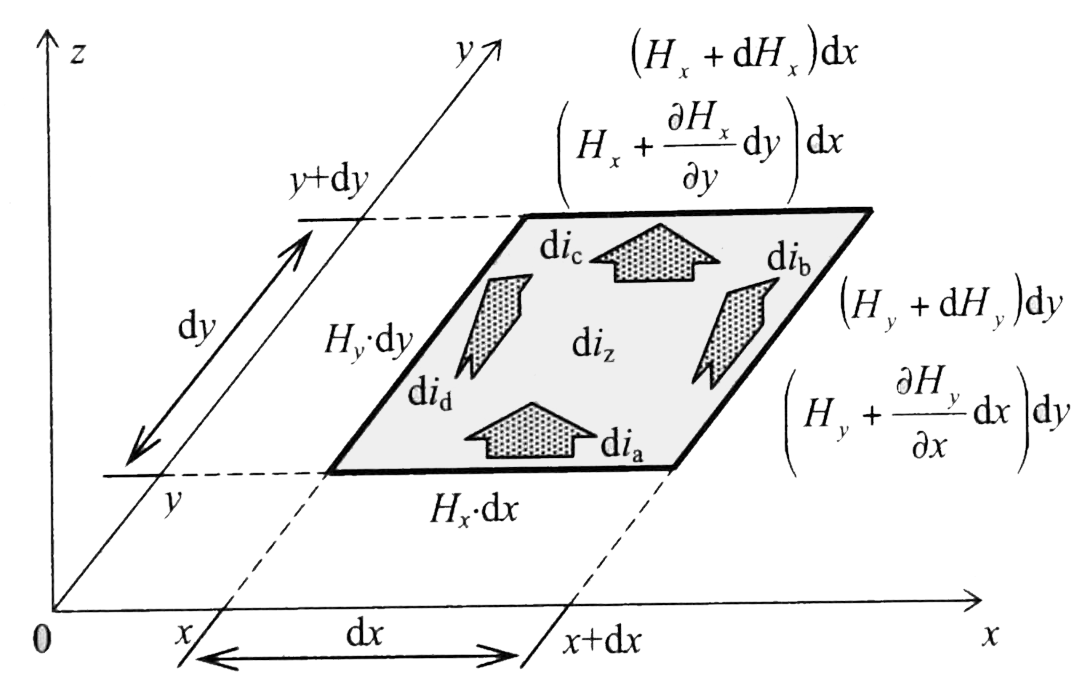
\includegraphics[width=0.8\linewidth]{patocka_mag_tok_exp12.png}
        \caption{Geometrická interpretace \emph{z}-složky \((\rot{H}_z)\) vektoru \(\rot{H}\).}
        \label{es:fig_patocka_mag_tok_exp12}
      \end{figure}
      Geometrický význam \emph{z}-složky \((\rot{H}_z)\) je zřejmý z obr. 
      \ref{es:fig_patocka_mag_tok_exp12}. Jedná se o podobnou situaci, jaká je zobrazena na Obr. 
      \ref{ES:fig_patocka_mag_tok_exp11a}. S ohledem na diferenciální velikost plochy \(dS_z\) je 
      totiž nutno proudy \(di_a, di_b\) ... chápat jako \emph{spojitě rozprostřené} v ploše 
      \(dS_z\), nikoli jako bodové (menší plocha než \(dS_z\) totiž neexistuje). Elementární proud 
      \(di_z = di_a + di_b + di_c + di_d\) tekoucí diferenciální smyčkou \(dS_z\) se nazývá 
      \textbf{ elementární cirkulací} vektoru \(\vec{H}\).

  \section{Třetí Maxwellova rovnice}\label{ES:sec08}
    Konstrukce třetí Maxwellovy rovnice je založena na pojmu \emph{divergence vektoru}, proto je 
    nezbytné nejdříve se s tímto pojmem seznámit.
    
    \subsection{Divergence vektoru D}\label{ES:ssec01}
      Elektrická indukce \(\vec{D}\) je \emph{vektor}, který má význam lokální \emph{plošné 
      hustoty} \(d\Psi_D/dS\) dielektrického toku \(\Psi_D\) neboli plošné hustoty \(dQ/dS\) náboje 
      \(Q\), protože platí identita \(\Psi\equiv Q\).
      
      Naproti tomu divergence \(\diver{D}\) vektoru je \emph{skalár}, který má význam lokální 
      \emph{objemové hustoty} \(\varrho\) náboje. Chceme-li získat objemovou hustotu \(\varrho\) 
      náboje, musíme každou složku \(D_x, D_y , D_z\) indukce \(\vec{D}\) derivovat podle příslušné 
      proměnné \(x, y, z\). Derivace totiž určuje \emph{přírůstek indukce} a ten musí být způsoben 
      \emph{výskytem lokálního náboje} v daném diferenciálním objemu \(dV\). Pro složku \(D_x\) 
      vektoru \(\vec{D}\) zřejmě podle obr. \ref{es:fig_patocka_mag_tok_exp13} platí:
      \begin{equation}\label{ES:eq_zakl_elm46}
        D_x = \frac{d\Psi_{D_x}}{dS_x} = \frac{d\Psi_{D_x}}{\dd{y}\,\dd{z}} = \frac{dQ_x}{\dd{y}\,\dd{z}}. 
      \end{equation} 
      Divergenci ve směru \(x\) získáme tak, že složku indukce \(D_x\) derivujeme podle příslušné 
      proměnné \(x\). S pomocí rovnice (\ref{ES:eq_zakl_elm46}) lze derivaci \(\frac{dD_x}{\dd{x}}\) 
      vyjádřit ve tvaru
      \begin{equation}\label{ES:eq_zakl_elm47}
        (\diver{D})_x = \frac{dD_x}{dS_x} = \frac{dQ_x}{\dd{x}\dd{y}\dd{z}} = \frac{dQ_x}{dV} = \varrho_x. 
      \end{equation} 
      Podobně můžeme získat složky divergence ve zbývajících směrech. Z rovnice 
      (\ref{ES:eq_zakl_elm47}) vyplývá, jak souvisí přírůstek indukce \(dD_x\) s objemovou hustotou 
      \(\varrho_x\) náboje a s divergenci. Na výstupu elementární krychle bude mít přírůstek 
      indukce ve směru \(x\) velikost
      \begin{equation}\label{ES:eq_zakl_elm48}
        dD_x = \varrho_x\,\dd{x} = (\diver{D})_x\,\dd{x} = \pder{D_x}{x}\,\dd{x}. 
      \end{equation} 
      \begin{figure}[ht!]
        \centering
        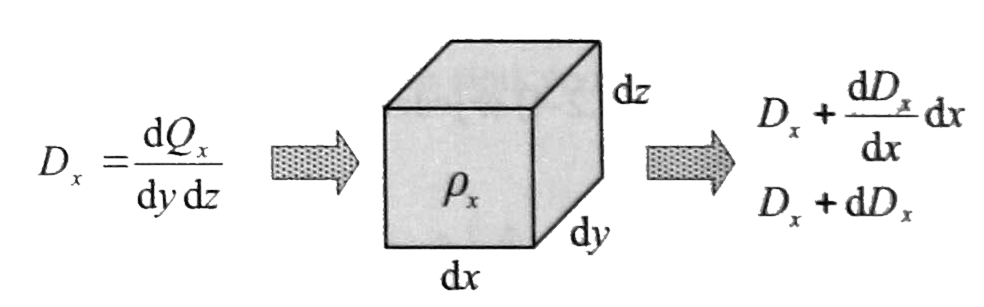
\includegraphics[width=0.9\linewidth]{patocka_mag_tok_exp13.png}
        \caption{Vztah mezi složkou elektrické indukce \(D_x\) a objemovou hustotou \(\varrho_x\) 
                 náboje.}
        \label{es:fig_patocka_mag_tok_exp13}
      \end{figure}
      
      Hustota náboje je \emph{skalární aditivní} veličina. Proto musíme algebraicky sečíst 
      příspěvky \(\varrho_x, \varrho_y, \varrho_z\) ode všech složek divergence ve směrech \(x, y, 
      z\), abychom získali celkovou hustotu \(\varrho\) náboje v elementárním objemu. Celkové 
      hustotě bude rovna i celková divergence v daném bodě:
      \begin{align}\label{ES:eq_zakl_elm49}
        \diver{D} &= (\diver{D})_x + (\diver{D})_y + (\diver{D})_z  \nonumber \\
                  &= \pder{D_x}{x} + \pder{D_y}{y} + \pder{D_z}{z} =
                     \varrho_x + \varrho_y + \varrho_z = \varrho. 
      \end{align} 
      Objemová hustota náboje, tedy i divergence, jsou \emph{skalární} veličiny.
      
    \subsection{Konstrukce třetí Maxwellovy rovnice}\label{ES:ssec02}
      Rovnice (\ref{ES:eq_zakl_elm49}) je přímo III. Maxwellovou rovnicí v diferenciálním tvaru:
      \begin{equation}\label{ES:eq_zakl_elm50}
        \diver{D} = \varrho \qquad [C/m^2, 1/m; C/m^3]. 
      \end{equation} 
      \begin{figure}[ht!]
        \centering
        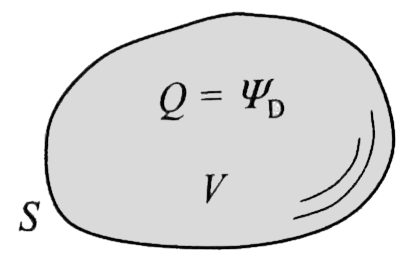
\includegraphics[width=0.4\linewidth]{patocka_mag_tok_exp14.png}
        \caption{Uzavřená orientovaná plocha \(S\) (např. koule) tvoří hranici vnitřního prostoru o 
                 objemu \(V\). Ve vnitřním prostoru se nachází náboj \(Q\).}
        \label{es:fig_patocka_mag_tok_exp14}
      \end{figure}
      
      Plocha \(S\) na obr \ref{es:fig_patocka_mag_tok_exp14} tvoří hranici vnitřního prostoru o 
      objemu \(V\). Z topologického hlediska se jedná o plochu \emph{neohraničenou} (nemá hraniční 
      křivku \(l\)) a \emph{orientovanou} (vnitřní stěnu lze natřít zeleně \textbf{z}, vnější 
      červeně \textbf{č}). Příkladem plochy může být \emph{koule}. Celkový dielektrický tok 
      \(\Psi_D\) prostupující plochou je roven celkovému náboji \(Q\) uvnitř plochy. Pro tok 
      \(\Psi_D\) platí analogie rovnic (\ref{ES:eq_zakl_elm12}), (\ref{ES:eq_zakl_elm39}), a to 
      včetně věty \ref{es:fig_patocka_lemma01} o nezávislosti integrálu na tvaru plochy:
      \begin{equation}\label{ES:eq_zakl_elm51}
        \Psi_D \equiv Q = \int_S\vec{D}\cdot \dd{\vec{S}}.
      \end{equation} 
      Plošný integrál (\ref{ES:eq_zakl_elm51}) převedeme pomocí \textbf{Gaussovy 
      věty}\footnote{Gaussovu větu vysvětlíme v následující kapitole} na integrál objemový:
      \begin{equation}\label{ES:eq_zakl_elm52}
        \Psi_D \equiv Q = \int_S\vec{D}\cdot \dd{\vec{S}} = \int_V\diver{D}\,dV.
      \end{equation} 
      Do rovnice (\ref{ES:eq_zakl_elm52}) dosadíme místo divergence \(\diver{D}\) pravou stranu 
      rovnice (\ref{ES:eq_zakl_elm50}), tj. nábojovou hustotu \(\varrho\). Tak získáme \emph{III. 
      Maxwellovu rovnici} v \emph{integrálním} tvaru
      \begin{equation}\label{ES:eq_zakl_elm53}
        \boxed{\int_S\vec{D}\cdot \dd{\vec{S}} = \int_V\varrho\,dV}.
      \end{equation} 
      Zdůrazněme, že na levé straně rovnice (\ref{ES:eq_zakl_elm53}) se jedná o skalární součin 
      dvou vektorů, na pravé straně o prostý součin dvou skalárů.
      
    \subsection{Gaussova věta}
      Plocha \(S\) tvoří podle obr. \ref{es:fig_patocka_mag_tok_exp14} hranici vnitřního prostoru o 
      objemu \(V\). Z topologického hlediska se jedná o plochu \emph{neohraničenou} a 
      \emph{orientovanou} (např. koule). Gaussova\footnote{Carl Fridrich Gauss (1777-1855), 
      vynikající matematik a fyzik, působil na univerzitě v Gottingenu. Kromě matematiky a 
      elektřiny se zabýval např. teorií geomagnetismu. Společně s W. E. Weberem sestrojili r. 1833 
      první telegraf.}  věta obecně převádí plošný integrál přes tuto plochu \(S\) na objemový 
      integrál přes objem \(V\). Pro pochopení věty velice pomáhá konkrétní fyzikální interpretace 
      jednotlivých veličin. Proto budeme větu zkoumat v konkrétním případě pro vektor indukce 
      \(\vec{D}\). Pak má věta tvar
      \begin{equation}\label{ES:eq_zakl_elm54}
        \int_S\vec{D}\cdot \dd{\vec{S}} = \int_V\diver{D}\,dV \quad(=Q).
      \end{equation} 
      Jak plyne z rovnic (\ref{ES:eq_zakl_elm51}), (\ref{ES:eq_zakl_elm52}), obě strany rovnice 
      (\ref{ES:eq_zakl_elm54}) mají význam celkového náboje \(Q\) uzavřeného uvnitř plochy. Důkaz 
      věty lze konstruovat tak, že \emph{trojný objemový} integrál na pravé straně rovnice 
      (\ref{ES:eq_zakl_elm54}) se budeme snažit převést nezávislým matematickým postupem na dvojný 
      plošný integrál. Z rovnice (\ref{ES:eq_zakl_elm49}) plyne
      \begin{equation}\label{ES:eq_zakl_elm55}
        \varrho = \varrho_x + \varrho_y + \varrho_z 
                = \der{D_x}{x} + \der{D_y}{y} + \der{D_z}{z}. 
      \end{equation}
      Pravou stranu rovnice (\ref{ES:eq_zakl_elm54}) vyjádříme ve tvaru trojného integrálu a 
      dosadíme do ní místo \(\varrho\) pravou stranu rovnice (\ref{ES:eq_zakl_elm55}):
      \begin{align}\label{ES:eq_zakl_elm56}
        Q &= \int_V\diver{D}dV = \int_V\varrho dV 
           = \limitint_{\mathclap{x_Vy_Vz_V}}\varrho\,\dd{x}\,\dd{y}\,\dd{z}   \nonumber\\
          &= \limitint_{\mathclap{x_Vy_Vz_V}}\left(dD_x\,\dd{y}\,\dd{z}+dD_y\,\dd{x}\,\dd{z}+dD_z\,\dd{x}\,\dd{y}\right).
      \end{align}      
      \begin{figure}[ht!]
        \centering
        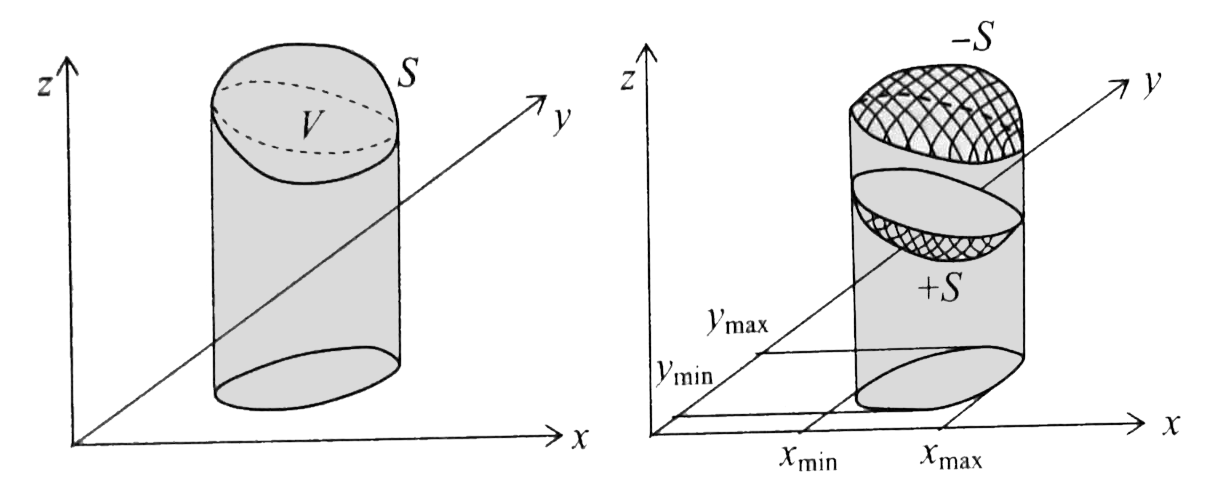
\includegraphics[width=0.9\linewidth]{patocka_mag_tok_exp15.png}
        \caption{Průmět uzavřené plochy \(S\) do roviny \emph{x-y}. Průměty do roviny \emph{y-z, 
                 z-x} lze získat podobně.}
        \label{es:fig_patocka_mag_tok_exp15}
      \end{figure}
      Integrační meze \(x_Vy_Vz_V\) odpovídají podle obr. \ref{es:fig_patocka_mag_tok_exp15} 
      průmětům prostoru \(V\) do příslušných souřadných rovin a z nich do příslušných souřadných 
      os. Zřejmě platí
      \begin{equation}\label{ES:eq_zakl_elm57}
        \limitint_{\mathclap{x_V}}dD_x = D_x \qquad
        \limitint_{\mathclap{y_V}}dD_y = D_y \qquad
        \limitint_{\mathclap{z_V}}dD_z = D_z.
      \end{equation}
      Po dosazení rovnic (\ref{ES:eq_zakl_elm57}) do (\ref{ES:eq_zakl_elm56}) získáme výraz
      \begin{align}\label{ES:eq_zakl_elm58}
        Q &= \iiint\limits_{x_Vy_Vz_V}\varrho\,\dd{x}\,\dd{y}\,\dd{z}   \nonumber\\ 
          &= \iint\limits_{y_Vz_V}D_x\,\dd{y}\,\dd{z} + 
             \iint\limits_{z_Vx_V}D_y\,\dd{z}\,\dd{x} + 
             \iint\limits_{x_Vy_V}D_z\,\dd{x}\,\dd{y}               \nonumber\\ 
          &= \int\limits_{S_x}D_x\,dS_x + 
             \int\limits_{S_y}D_y\,dS_y + 
             \int\limits_{S_z}D_z\,dS_z =  \int\limits_{S}\vec{D}\cdot\vec{S}
      \end{align}
      Ve třech dílčích integrálech nefiguruje součin skalární, nýbrž součin prostý (jedná se o 
      složky vektoru, nikoli o vektor). Integrační meze \(S_x, S_y, S_z\) mají význam 
      \emph{průmětů} plochy \(S\) do jednotlivých souřadných rovin \(y-z\), \(z-x\), \(x-y\). 
      Protože je plocha \(S\) uzavřená, v příslušné rovině existují vždy dva různé průměty: 
      \(S_{+x}, S_{-x}, S_{+y}, S_{-y}, S_{+z}, S_{-z}\). Těm odpovídají dvě různé indukce: 
      \(D_{+x}, D_{-x}, D_{+y}, D_{-y}, D_{+z}, D_{-z}\). V rovnici (\ref{ES:eq_zakl_elm58}) se 
      tedy ve skutečnosti objeví šest dílčích plošných integrálů, uspořádaných do tří dvojic:
      \begin{align*}   %\label{ES:eq_zakl_elm59}
        Q  = \iiint\limits_{x_Vy_Vz_V}\varrho\,\dd{x}\,\dd{y}\,\dd{z}   
          &= \int\limits_{S_x}D_x\,dS_x + 
             \int\limits_{S_y}D_y\,dS_y + 
             \int\limits_{S_z}D_z\,dS_z                                                \\
          &= \int\limits_{S_{+x}}D_{+x}\,dS_x - \int\limits_{S_{-x}}D_{-x}\,dS_x       \\
          &+ \int\limits_{S_{+y}}D_{+y}\,dS_y - \int\limits_{S_{-y}}D_{-y}\,dS_y       \\
          &+ \int\limits_{S_{+z}}D_{+z}\,dS_z - \int\limits_{S_{-z}}D_{-z}\,dS_z       \\
          &= \underbrace{\iint\limits_{y_Vz_V}D_{+x}\,\dd{y}\,\dd{z} 
           - \iint\limits_{y_Vz_V}D_{-x}\,\dd{y}\,\dd{z}}_{\text{dva průměty do roviny y-z}}   \\
          &+ \underbrace{\iint\limits_{z_Vx_V}D_{+y}\,\dd{z}\,\dd{x} 
           - \iint\limits_{z_Vx_V}D_{-y}\,\dd{z}\,\dd{x}}_{\text{dva průměty do roviny z-x}}   \\
          &+ \underbrace{\iint\limits_{x_Vy_V}D_{+z}\,\dd{x}\,\dd{y} 
           - \iint\limits_{x_Vy_V}D_{-z}\,\dd{x}\,\dd{y}}_{\text{dva průměty do roviny x-y}}
      \end{align*}
      Záporná znaménka u sudých integrálů plynou z faktu, že plochy ve dvojici příslušných průmětů 
      jsou opačně orientovány (\textbf{č}\(\rightarrow\)\textbf{z}, 
      \textbf{z}\(\rightarrow\)\textbf{č}). Trojný objemový integrál se tedy podařilo převést 
      na integrál dvojný plošný. Tím je důkaz věty dokončen.
      
  \section{Čtvrtá Maxwellova rovnice}\label{ES:sec09}
    Postup při odvození IV. Maxwellovy rovnice je formálně naprosto shodný s postupem v předchozích 
    kapitolách \ref{ES:ssec01}. a \ref{ES:ssec01}. Ve všech rovnicích pouze nahradíme 
    \emph{elektrické} veličiny analogickými veličinami \emph{magnetickými}, tj. \(D\rightarrow 
    B\), \(\Psi_D\rightarrow \Psi\), \(\varrho\rightarrow \varrho_m\). Proto budou oba 
    tvary IV. MR formálně podobné tvarům III. MR, tj. rovnicím (\ref{ES:eq_zakl_elm53}), 
    (\ref{ES:eq_zakl_elm53}). Velký rozdíl je ale v tom, že elektrické pole je \emph{zřídlové}, 
    kdežto magnetické pole je \emph{vírové}. Z topologického pohledu to znamená:
    \begin{itemize}[noitemsep]
      \item Siločáry elektrické intenzity \(\vec{E}\) nebo \(\vec{D}\) jsou \emph{neuzavřené} 
            křivky, které mají začátek ve „zřídlu“ +Q a konec ve „zřídlu“ -Q.
    
      \item Siločáry magnetické intenzity \(\vec{H}\) nebo \(\vec{B}\) jsou naopak \emph{uzavřené} 
            křivky (tj. „víry“), které  nemají ani začátek ani konec, protože neexistuje magnetický 
            náboj v podobě magnetického monopolu. V magnetismu tedy neexistuje analogie v podobě 
            „+zřídla“ a „-zřídla“. Odtud plyne, že objemová hustota magnetických monopolů 
            \(\varrho_m\) je vždy \emph{nulová}, proto musí být v obou rovnicích položeno 
            \(\varrho_m = 0\).
    \end{itemize}
    \emph{Diferenciální tvar} IV. Maxwellovy rovnice tedy bude:
    \begin{equation}\label{ES:eq_zakl_elm60}
      \diver{B} = 0 \qquad [Wb/m^2,1/m; Wb/m^3].
    \end{equation}
    \emph{Integrální tvar} IV. Maxwellovy rovnice bude:
    \begin{equation}\label{ES:eq_zakl_elm61}
      \int_S\vec{B}\cdot \dd{\vec{S}} = 0.
    \end{equation}    
    V rovnici (\ref{ES:eq_zakl_elm61}) se vždy jedná o \emph{uzavřenou neohraničenou orientovanou} 
    plochu \(S\) (např. kouli, jež má vnitřní stěnu natřenu zeleně \textbf{z}, vnější stěnu červeně 
    \textbf{č}), která tvoří hranici vnitřního prostoru o objemu \(V\), viz obr. 
    \ref{ES:fig_patocka_mag_tok_exp16}. Ve vnitřním prostoru se nemůže nacházet magnetický náboj 
    \(Q_m = \Psi\) v podobě magnetického monopolu - chybí tam zdroj siločar.
   
    \begin{figure}[ht!]
      \centering  
      \subcaptionbox{\label{ES:fig_patocka_mag_tok_exp16a}}{\luafigure[0.45]{patocka_mag_tok_exp16a.png}}
      \subcaptionbox{\label{ES:fig_patocka_mag_tok_exp16b}}{\luafigure[0.45]{patocka_mag_tok_exp16b.png}}
      \caption{Uzavřená orientovaná plocha \(S\) tvořící hranici vnitřního prostoru \(V\): a)   
               ve vnitřním prostoru se nemůže nacházet magnetický náboj \(Q_m = \Phi\) v podobě 
               magnetického monopólu, b) vnější tok vstupuje do vnitřního prostoru levou části 
               plochy ve směru \textbf{č\(\rightarrow\)z} a vystupuje pravou částí ve směru 
               \textbf{z\(\rightarrow\)č}.} 
      \label{ES:fig_patocka_mag_tok_exp16}
    \end{figure}

    Všechny vnější siločáry vstupují do vnitřního objemu částí plochy ve směru 
    \textbf{č}\(\rightarrow\)\textbf{z} a vystupují ven zbývající částí ve směru 
    \textbf{z}\(\rightarrow\)\textbf{č}. Tyto dvě části lze od sebe formálně oddělit uzavřenou 
    křivkou \(l\), která tvoří přirozenou hranici mezi těmito dvěma oblastmi - jedná se o 
    geometrické místo tečných bodů, v nichž se některé ze siločar pouze tečné dotknou plochy \(S\), 
    aniž ji protnou. Pak je možno na problém aplikovat větu \ref{es:fig_patocka_lemma01}: Integrál 
    přes oblast \textbf{č}\(\rightarrow\)\textbf{z} musí mít v absolutní hodnotě stejnou 
    velikost jako integrál přes oblast \textbf{z}\(\rightarrow\)\textbf{č}. S ohledem na opačné 
    orientace však musí mít oba integrály navzájem opačná znaménka. Proto musí platit:
    \begin{equation}\label{ES:eq_zakl_elm62}
      \int\limits_{S}\vec{B}\cdot \dd{\vec{S}} = 
      \int\limits_{\text{č}\rightarrow\text{z}}\vec{B}\cdot \dd{\vec{S}} -
      \int\limits_{\text{z}\rightarrow\text{č}}\vec{B}\cdot \dd{\vec{S}} = 0.
    \end{equation} 
    Celkový tok plochou \(S\) je tedy opravdu nulový.
    
  \section{Biotův-Savartův zákon}\label{ES:sec10}
    Oersted\footnote{Hans Christian Oersted (1777-1851), fyzik a chemik, působil na univerzitě v 
    Kodani. Ve víře v jednotnou přírodní sílu hledal souvislosti mezi přírodními jevy na první 
    pohled nesouvisejícími.} zveřejnil v roce 1820 své experimentální výsledky, týkající se 
    silového působení elektrického proudu na magnetku kompasu. Jeho výsledky však byly pouze 
    kvalitativní. Zanedlouho poté odvodili Biot\footnote{Jean Baptisté Biot (1774-1862), fyzik, 
    působil na Sorboně. Zabýval se elektrodynamikou a optikou.} se Savartem\footnote{Felix Savart 
    (1791-1841), lékař, později působil jako fyzik na Sorboně. Zabýval se elektrodynamikou a 
    akustikou.} na základě složitých experimentů kvantitativní vztah pro výpočet síly působící na 
    magnetku, který upravil Laplace do tvaru
    \begin{equation}\label{ES:eq_zakl_elm63}
      d\vec{F} = KI\frac{\dd{\vec{l}}\times \vec{r}}{r^3}
    \end{equation} 
    
    Konstanta \(K\) v Laplaceově\footnote{Pierre-Simon Laplace (1749-1827), matematik a astronom, 
    člen francouzské Akademie věd. Zabýval se mechanikou a gravitační stabilitou sluneční soustavy, 
    teorií potenciálu, je zakladatelem integrálních transformací v matematice.} rovnici je závislá 
    na použité soustavě jednotek. Zákon říká, že každá elementární část vodiče o diferenciální 
    délce \(dl\) působí na magnetku diferenciálním přírůstkem síly \(dF\). Oersted však zjistil, že 
    vodič \(L\) působí zcela stejně nejen na magnetku, ale i na malý kruhový závit, kterým protéká 
    jiný nezávislý proud. Na základě tohoto experimentálního faktu bylo možno o několik let 
    později, až po zavedení pojmu \emph{„magnetické pole“} Faradayem, modifikovat Biotův-Savartův 
    zákon do současné podoby. Současný tvar zákona, daný rovnicí (\ref{ES:eq_zakl_elm63}), umožňuje 
    výpočet magnetického pole \(H\) nebo \(B\), generovaného vodičem libovolného tvaru, v 
    libovolném bodě prostoru. Prostor ale musí být vyplněn magneticky \emph{izotropním, homogenním 
    a lineárním} prostředím. Předpokladem je, že tloušťka vodiče je zanedbatelná vůči rozměrům 
    vyšetřovaného prostoru. Zákon říká, že každá část vodiče o diferenciální délce \(dl\) vytváří 
    ve sledovaném bodě diferenciální přírůstek magnetického pole \(dH\), resp. \(dB\) podle rovnice
    \begin{equation}\label{ES:eq_zakl_elm64}
      d\vec{H} = \frac{I}{4\pi}\frac{\dd{\vec{l}}\times \vec{r}}{r^3}, \qquad\text{resp.}\qquad
      d\vec{B} = \mu_0\frac{I}{4\pi}\frac{\dd{\vec{l}}\times \vec{r}}{r^3}.
    \end{equation}     
    \begin{figure}[ht!]
      \centering
      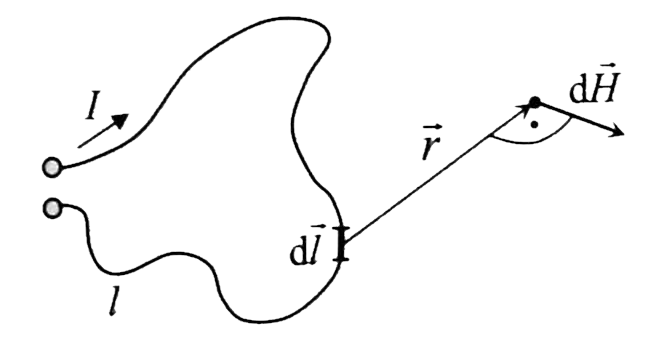
\includegraphics[width=0.5\linewidth]{patocka_mag_tok_exp17.png}
      \caption{K Biotovu-Savartovu zákonu.}
      \label{es:fig_patocka_mag_tok_exp17}
    \end{figure}
    Celkové pole v tomtéž sledovaném bodě lze určit integrací diferenciálních přírůstků 
    (\ref{ES:eq_zakl_elm64}), způsobených všemi diferenciálními částmi \(dl\) vodiče. Konečná 
    podoba Biotova-Savartova zákona má tvar křivkového integrálu, přičemž integrační křivka \(l\) 
    je určena tvarem vodiče:
    \begin{equation}\label{ES:eq_zakl_elm65}
      \vec{H} = \frac{I}{4\pi}\int_l\frac{\dd{\vec{l}}\times \vec{r}}{r^3}, \quad\text{resp.}\quad
      \vec{B} = \mu_0\frac{I}{4\pi}\int_l\frac{\dd{\vec{l}}\times \vec{r}}{r^3}.
    \end{equation} 
    
    Pro obecný tvar vodiče je výpočet křivkového integrálu tak složitý, že je obvykle v uzavřeném 
    tvaru neřešitelný. Snadno řešitelný je však ve \emph{zvláštních případech}, které vykazují 
    vhodnou geometrickou symetrii.
    
    Jedním z nich je výpočet pole \emph{přímého nekonečně dlouhého vodiče}. Je známo, že pole 
    \(\vec{H}\) takového vodiče je kruhově symetrické podle obr. 
    \ref{es:fig_patocka_mag_tok_exp18}. Pro bod umístěný ve vzdálenosti \(R\) od vodiče lze 
    druhou rovnici (\ref{ES:eq_zakl_elm64}) modifikovat do tvaru      
    \begin{figure}[ht!]
      \centering
      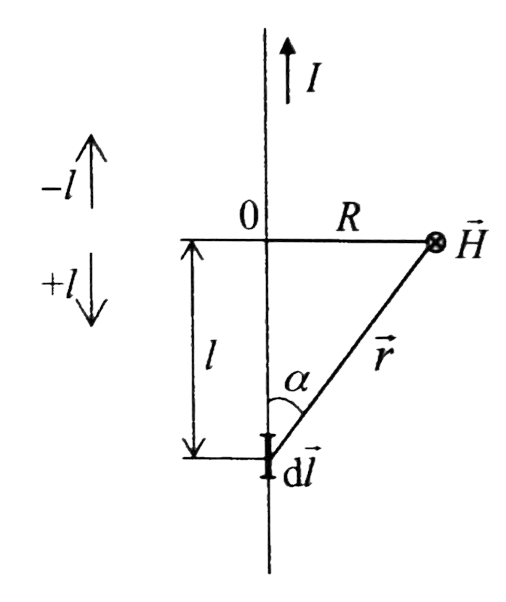
\includegraphics[width=0.4\linewidth]{patocka_mag_tok_exp18.png}
      \caption{K výpočtu pole přímého nekonečně dlouhého vodiče pomocí Biotova-Savartova zákona.}
      \label{es:fig_patocka_mag_tok_exp18}
    \end{figure}
    \begin{align}\label{ES:eq_zakl_elm66}
      d\vec{H} &= \frac{I}{4\pi}\frac{dl\,r\sin\alpha}{r^3}
                = \frac{I}{4\pi}\frac{dl\sin\alpha}{r^2}                 \nonumber \\
               &= \frac{I}{4\pi}\frac{Rdl}{r^3}
                = \frac{IR}{4\pi}\frac{dl}{\left(r^2+l^2\right)^{\frac{3}{2}}}
    \end{align}
    Podle rovnice (\ref{ES:eq_zakl_elm65}) pro \(\vec{H}\) bude mít intenzita magnetického pole 
    velikost 
    \begin{align}\label{ES:eq_zakl_elm67}
      \vec{H} &= \frac{IR}{4\pi}\int\limits_{-\infty}\limits^{+\infty}
                 \frac{dl}{\left(r^2+l^2\right)^{\frac{3}{2}}}
               = \frac{IR}{4\pi} 
                 \left[\frac{l}{R^2\sqrt{R^2+l^2}}\right]_{-\infty}^{+\infty}         \nonumber \\
              &= \frac{I}{4\pi R}
                 \left[\frac{1}{\sqrt{\dfrac{R^2}{l^2}+1}}\right]_{-\infty}^{+\infty} \nonumber \\
              &= \frac{I}{4\pi R}[1-(-1)] = \frac{I}{2\pi R}
    \end{align}
    Poznamenejme, že po krácení zlomku v prvních hranatých závorkách veličinou \(l\) nesmí 
    zaniknout informace o znaménku veličiny \(l\). Proto musí být hodnota následného zkráceného 
    zlomku ve druhých hranatých závorkách po dosazení dolní meze \emph{záporná}, po dosazení horní 
    meze \emph{kladná}. Takto jsme dospěli ke známému výsledku pro intenzitu magnetického pole 
    přímého dlouhého vodiče. Této intenzitě odpovídá magnetická indukce
    \begin{equation}\label{ES:eq_zakl_elm68}
      B = \mu_0H = \mu_0\frac{I}{2\pi R}
    \end{equation}
    
    Jiným zvláštním případem, vykazujícím geometrickou symetrii, je výpočet pole v rotační ose 
    kruhového závitu nebo válcové cívky ( např. \emph{Helmholtzovy cívky}). 
    
  \section{Elektromagnetické síly}\label{ES:sec11}
    Cílem této kapitoly je ukázat jednotné fyzikální principy vedoucí ke vzniku mechanických sil.
    
    \subsection{Vznik mechanických sil v elektromagnetickém poli}
      Koná-li síla \(F\) práci na dráze \(l\) a mění-li během pohybu svoji velikost, nelze použít k 
      výpočtu mechanické práce rovnici \(W_{mech}= Fl\), nýbrž je nutno použít její diferenciální 
      obdobu
      \begin{equation}\label{ES:eq_zakl_elm69}
        dW_{mech} = Fdl
      \end{equation}
      
      Platnost rovnice je založena na základním principu diferenciálního počtu, který říká, že v 
      limitním případě, na diferenciální dráze \(dl\), musí být síla \(F\) \emph{konstantní}. S 
      ohledem na \emph{limitně nulovou} délku dráhy \(dl\) se diferenciální přírůstek vykonané 
      práce \(dW_{mech}\) též někdy nazývá \textbf{virtuální prací}. Virtuální práce \(dW_{mech}\), 
      vykonaná izolovanou fyzikální soustavou, musí být kryta ze zdroje energie energetickým 
      příspěvkem \(dW\), a to takovým způsobem, aby \emph{celková energie soustavy zůstala 
      zachována}. Odtud plyne, že součet diferenciálních energetických přírůstků v izolované 
      soustavě musí být nulový:
      \begin{equation}\label{ES:eq_zakl_elm70}
        dW_{mech}+dW=0.
      \end{equation}
      Z rovnic (\ref{ES:eq_zakl_elm69}), (\ref{ES:eq_zakl_elm70}) plyne, že v soustavě nutně vzniká 
      mechanická síla
      \begin{equation}\label{ES:eq_zakl_elm71}
        \boxed{F = \frac{dW_{mech}}{dl} = -\frac{dW}{dl}},
      \end{equation}
      kde \(dW\) je přírůstek energie dodaný zdrojem.
      
      V případě elektromagnetu se železným jádrem a se vzduchovou mezerou lze zanedbat magnetickou 
      vodivost železa oproti vodivosti vzduchové mezery. Pak je veškerá magnetická energie 
      soustředěna pouze do objemu vzduchové mezery o délce \(l\):
      \begin{equation}\label{ES:eq_zakl_elm72}
        W =\frac{1}{2}Li^2 = \frac{1}{2}i^2N^2\mu_0\frac{S_{Fe}}{l}.
      \end{equation}
      Z rovnic (\ref{ES:eq_zakl_elm72}) a (\ref{ES:eq_zakl_elm71}) plyne, že ve vzduchové mezeře 
      magnetu vznikne síla
      \begin{align}\label{ES:eq_zakl_elm73}
         F = -\frac{dW}{dl} 
           &= +\frac{1}{2}i^2N^2\mu_0\frac{S_{Fe}}{l^2}
           =  \frac{1}{2}i^2\frac{L}{l} = \frac{1}{2}H^2\mu_0S_{Fe}              \nonumber \\
           &=  \frac{1}{2}BHS_{Fe} = \frac{1}{2}\frac{B^2}{\mu_0}S_{Fe}.
      \end{align}
      Mechanický tlak ve vzduchové mezeře bude
      \begin{equation}\label{ES:eq_zakl_elm74}
        p = \frac{F}{S_{Fe}} = \frac{1}{2}H^2\mu_0 = \frac{1}{2}BH = \frac{1}{2}\frac{B^2}{\mu_0}.
      \end{equation}
      Z rovnice (\ref{ES:eq_zakl_elm72}) rovněž vyplývá, že objemová hustota energie magnetického 
      pole ve vzduchové mezeře je \emph{identicky rovna} mechanickému tlaku:
      \begin{align}\label{ES:eq_zakl_elm75}
        w  = \frac{W}{V} 
          &= \frac{W}{S_{Fe}l} = \frac{1}{2}i^2N^2\mu_0\frac{1}{l^2}             \nonumber \\
          &= \frac{1}{2}H^2\mu_0 = \frac{1}{2}BH = \frac{1}{2}\frac{B^2}{\mu_0}.
      \end{align}
      Podobně v případě vzduchového kondenzátoru lze sílu určit pomocí elektrostatické energie 
      nashromážděné v prostoru mezi elektrodami:
      \begin{equation}\label{ES:eq_zakl_elm76}
        W = \frac{1}{2}u^2C = \frac{1}{2}u^2\varepsilon_0\frac{S}{l}.
      \end{equation}
      Z rovnic (\ref{ES:eq_zakl_elm76}) a (\ref{ES:eq_zakl_elm71}) plyne, že ve vzduchové mezeře 
      kondenzátoru vznikne síla
      \begin{align}\label{ES:eq_zakl_elm77}
        F  = \frac{dW}{dl} 
          &= \frac{1}{2}u^2\varepsilon_0\frac{S}{l^2}
           = \frac{1}{2}E^2\varepsilon_0S                                 \nonumber \\
          &= \frac{1}{2}DES           
           = \frac{1}{2}\frac{D^2}{\varepsilon_0}S.
      \end{align}
      Mechanický tlak mezi elektrodami kondenzátoru bude
      \begin{align}\label{ES:eq_zakl_elm78}
        F  = \frac{dW}{dl} 
          &= \frac{1}{2}u^2\varepsilon_0\frac{S}{l^2}
           = \frac{1}{2}E^2\varepsilon_0S                                 \nonumber \\
          &= \frac{1}{2}DES          
           = \frac{1}{2}\frac{D^2}{\varepsilon_0}S.
      \end{align}
      Z rovnice (\ref{ES:eq_zakl_elm76}) vyplývá, že objemová hustota energie elektrického pole 
      mezi elektrodami kondenzátoru je identicky rovna mechanickému tlaku:
      \begin{align}\label{ES:eq_zakl_elm79}
        w  = \frac{W}{V} 
          &= \frac{W}{Sl} 
           = \frac{1}{2}u^2\varepsilon_0\frac{1}{l^2}         \nonumber \\
          &= \frac{1}{2}E^2\varepsilon_0 = \frac{1}{2}DE 
           = \frac{1}{2}\frac{D^2}{\varepsilon_0}.
      \end{align}
      Je zajímavé, že v případě elektromagnetu i kondenzátoru je tlak ve vzduchové mezeře roven 
      objemové hustotě energie v téže mezeře, tj. \(p = w\).
      
      Pro dokreslení fyzikálních souvislostí porovnejme tento výsledek s termodynamikou plynů. U 
      plynu uzavřeného v nádobě se celková hustota kinetické energie molekul musí podle
      \emph{ekvipartičního teorému} rovnoměrně rozdělit mezi tři souřadné směry \(x, y, z\), proto 
      by tlak plynu na stěny nádoby měl být třetinový, ve skutečnosti je ze složitějších důvodů 
      dvoutřetinový oproti hustotě kinetické energie:
      \begin{equation}\label{ES:eq_zakl_elm80}
        p = \frac{2}{3}w
      \end{equation}
      V mezeře elektromagnetu i kondenzátoru vzniká tlak pouze v \emph{jediném} 
      směru\footnote{Předpokládáme, že pólové nástavce jsou v zákrytu. Při vychýleni jednoho z 
      nástavců do strany sice vznikne v mezeře i boční síla, ale to je zcela jiné geometrické 
      uspořádání, které neuvažujeme.}, proto platí \(p = w\). Nositelé \emph{elektromagnetických 
      silových interakcí} jsou fotony\footnote{Na této skutečnosti je založena Feynmanova teorie 
      kvantové elektrodynamiky.}. Ty plní ve vzduchové mezeře elektromagnetu nebo 
      kondenzátoru podobnou roli jako molekuly plynu v nádobě. Rozdíl je pouze v tom, že vznikající 
      síla je přitažlivá, nikoli odpudivá a že fotony působí v jediném směru (při dané geometrické 
      konfiguraci).
      
      Analogicky k rovnici (\ref{ES:eq_zakl_elm74}) lze určit mechanický tlak uvnitř železného 
      jádra elektromagnetu, lokalizovaný ve \emph{vnitřním objemu železa} o relativní permeabilitě 
      \(\mu_{r_{Fe}}\)
      \begin{equation}\label{ES:eq_zakl_elm81}
       p = \frac{1}{2}\frac{B^2}{\mu_0\mu_{r_{Fe}}}.
      \end{equation}
      Vnitřní mechanický tlak v železe je vnějšímu pozorovateli experimentálně nedostupný. Nicméně 
      existuje a vidíme, že je řádově 2000krát menší oproti tlaku v mezeře. Stejný je i poměr 
      hustot energií v železe a v mezeře. To nás plně oprávnilo k původnímu zanedbání železa při 
      výpočtu síly. Všimněme si, že při \emph{konstantním} toku \(\Phi = BS_{Fe} = \text{konst}\). 
      platí tyto zákonitosti:
      \begin{itemize}[noitemsep]
        \item Magnetická síla je tím menší, čím je permeabilita obvodu větší, viz rovnice     
              (\ref{ES:eq_zakl_elm81}).
        \item Magnetická síla je tím menši, čím je plocha \(S_{Fe}\) obvodu větší, viz rovnice 
              (\ref{ES:eq_zakl_elm73}). Zřejmě totiž platí \(F \cong B^2S_{Fe} = 
              \frac{\Phi^2}{S_{Fe}} = \frac{\text{konst.}}{S_{Fe}}\).
      \end{itemize}
      Obě zákonitosti lze zobecnit takto:
      \begin{itemize}[noitemsep]
        \item Magnetická síla, tedy i potenciální energie soustavy, je tím menší, čím větší je    
              magnetická vodivost obvodu.
        \item Tlakové pole vznikající v magnetickém obvodu zaujme vždy takové prostorové rozložení, 
              které se snaží zdeformovat obvod do tvaru, v němž je potenciální energie obvodu co 
              nejmenší\footnote{Z podobných důvodů působí síla na těleso umístěné v gravitačním 
              poli. Gravitační síla má takový směr. že se snaží zmenšit potenciální energii \(mgh\) 
              tělesa na nulu.}, tj. v němž je magnetická vodivost obvodu co největší.
      \end{itemize}
      
      V důsledku obou zobecněných zákonitostí vznikají následující jevy:
      \begin{itemize}[noitemsep]
        \item Je-li součástí obvodu vzduchová mezera, tlakové pole se snaží zkrátit její délku na 
              nulu.
        \item Proudovodič ve tvaru uzavřené smyčky, umístěný volně v prostoru, se tlakové pole   
              snaží \emph{roztáhnout} do co největší plochy, tj. napnout vodič do kružnice.
        \item Dva paralelní vodiče, kterými protékají proudy \emph{opačných} směrů, se 
              \emph{odpuzuji} (v podstatě se jedná o podlouhlou uzavřenou smyčku z předchozího 
              bodu). U transformátoru se odpuzuje sekundární vinutí od primárního (opačné směry 
              proudů). Podobně vzduchová cívka napájená střídavým proudem se odpuzuje od kovové 
              nemagnetické desky, ve které vznikají vířivé proudy.
        \item Dva paralelní vodiče, kterými protékají proudy \emph{souhlasných} směrů, se 
              \emph{přitahuji}. U transformátoru se vzájemně přitahují závity téhož vinutí.
      \end{itemize}
      
      Z uvedených skutečností je zřejmé, že existence magnetické síly nesouvisí s přítomností 
      železa. V magnetickém obvodu, obsahujícím společně železo i vzduchovou mezeru, plní železo 
      roli pouhého „soustřeďovače siločar“ do objemu vzduchové mezery. V mezeře se pak jedná o 
      silovou interakci čistě mezi magnetickým \emph{polem} a \emph{vakuem}. Pro lepší pochopení 
      elektromagnetických sil je vhodné nahlížet na vakuum jako na „pružný materiál“\footnote{Při 
      řešení teoretických fyzikálních problémů je často užitečný „inženýrský přistup“. Z 
      psychologických důvodů proto není na škodu považovat vakuum za plnohodnotný „konstrukční“ 
      materiál, u kterého známe s jistotou tři jeho materiálové konstanty: \(\varepsilon_0\), 
      \(\mu_0\) a měrnou hmotnost \(\varrho = 0\).}, který je magnetickým polem 
      deformován do takového tvaru, aby magnetická vodivost tohoto „materiálu“ byla co 
      \emph{největší}. Jinak řečeno, aktivní objem vakua je silou nucen zaujmout takový tvar, aby 
      celková potenciální energie pole byla co \emph{nejmenší}.
      
      V	případě \emph{rotačního} pohybuje možno modifikovat rovnici (\ref{ES:eq_zakl_elm71}) pro 
      výpočet \emph{momentu síly}. Stačí vynásobit obě strany rovnice délkou ramena \(r\), na němž 
      síla působí:
      \begin{equation*}
        Fr = \frac{dW_{mech}}{dl}r 
           = \frac{dW_{mech}}{\dfrac{dl}{r}} 
           = \frac{dW_{mech}}{d\alpha}
             \qquad \Longrightarrow
      \end{equation*}
      \begin{equation}\label{ES:eq_zakl_elm82}
        \boxed{M = \frac{dW_{mech}}{d\alpha} = \frac{dW}{d\alpha}}
      \end{equation}
      kde \(\alpha\) je úhel natočení. Rovnice je vhodná pro přímý výpočet momentu všech 
      \emph{reluktančních motorů}, jejichž princip je založen na tom, že magnetická vodivost 
      vzduchové mezery se výrazně mění s úhlem natočení hřídele.
      
      Rovnici (\ref{ES:eq_zakl_elm71}) lze interpretovat tak, že síla je rovna \emph{strmosti}, s 
      jakou se mění energie soustavy v závislosti na změně délkové souřadnice \(l\). Ve složitějším 
      geometrickém uspořádání soustavy lze rovnici (\ref{ES:eq_zakl_elm71}) zobecnit do vektorového 
      tvaru
      \begin{equation}\label{ES:eq_zakl_elm83}
       \vec{F} = -\vec{i}\frac{dW}{\dd{x}} -\vec{j}\frac{dW}{\dd{y}} -\vec{k}\frac{dW}{\dd{z}} 
               = - \grad{W},
      \end{equation}
      kde \(\vec{i}, \vec{j}, \vec{k},\) jsou jednotkové vektory ve směru příslušných os. Síla je 
      pak nejobecněji definována jako záporně vzatý gradient (vektor) ze skalární funkce 
      \(W(x,y,z)\).
      
    \subsection{Lorentzova síla}
      
      Elektromagnetické síly působící na elektrický náboj lze shrnout do jediné Lorentzovy rovnice
      \begin{equation}\label{ES:eq_zakl_elm84}
        \vec{F}=q(\vec{E}+\vec{v}\times\vec{B}),
      \end{equation}
      ve které první člen vyjadřuje Coulombovu\footnote{Charles Augustin de Coulomb (1736-1806), 
      absolvent vojenské školy v Paříži. Zákon síly mezi dvěma bodovými náboji odhalil v období 
      1785 až 1789 v soukromí. Později jmenován členem pařížské Akademie věd.} elektrostatickou 
      sílu, působící na náboj \(Q\) umístěný v elektrickém poli \(\vec{E}\) a druhý člen vyjadřuje 
      Lorentzovu\footnote{Henrik Antoon Lorentz (1853-1928), teoretický fyzik, působil na 
      univerzitě v Leidenu. R. 1902 obdržel Nobelovu cenu za fyziku.} sílu, která působí na 
      náboj, pohybující se relativní rychlostí \(v\) vůči magnetickému poli \(B\). Lorentz 
      formuloval obě složky síly zcela obecně, tj. pro náboj pohybující se i relativistickou 
      rychlostí \(v \rightarrow c\), a to pomocí známých Lorentzových transformací. Pro 
      dokreslení historických souvislostí lze dodat, že Coulombův zákon pro náboje pohybující se 
      nižšími nerelativistickými rychlostmi korigoval už Weber ve druhé polovině 19. stol.
      a elektrické pole E, vytvořené relativisticky se pohybujícím nábojem, odvodil 
      Heaviside\footnote{Oliver Heaviside (1850-1925), technik britské telegrafní společnosti, 
      vynálezce duplexního telegrafu. Později soukromý vědec, samouk.} již r. 1888, tj. 17 let před 
      vznikem speciální teorie relativity. 
      
      V běžné inženýrské praxi lze zcela zanedbat Coulombovy síly oproti silám Lorentzovým. Navíc 
      je průměrná transportní (nikoli okamžitá) rychlost volných elektronů v kovech velmi malá, 
      řádově dosahuje \si{\cm/\s}, tudíž není nutno uvažovat relativistické efekty. Pak 
      můžeme uvažovat pouze druhý člen v rovnici (\ref{ES:eq_zakl_elm84}), pomocí něhož lze snadno 
      odvodit elementární Lorentzovu sílu \(dF\), působící na vodič o diferenciální délce \(dl\), 
      který se nachází v magnetickém poli \(B\).
       
      Protéká-li vodičem proud \(I\), z rovnice plyne:
      \begin{equation}\label{ES:eq_zakl_elm85}
        d\vec{F} =  dQ\,\vec{v}\times\vec{B} 
                 = I\dd{t}\,\vec{v}\times\vec{B} 
                 = I\dd{t}\,\frac{\dd{\vec{l}}}{\dd{t}}\times\vec{B}
                 = I\,\vec{l}\times\vec{B}.
      \end{equation}
      Díky vektorovému součinu je síla \(d\vec{F}\) vždy \emph{kolmá} na oba vektory \(\dd{\vec{l}}\) a 
      \(\vec{B}\) a v absolutní hodnotě má velikost
      \begin{equation}\label{ES:eq_zakl_elm86}
              dF=I\,dl\,B\sin\alpha,
      \end{equation}
      kde \(\alpha\) je úhel sevřený oběma vektory \(\dd{\vec{l}}\) a \(\vec{B}\). Proto musí všechny 
      tři vektory v pořadí \(\dd{\vec{l}}\), \(\vec{B}\), \(d\vec{F}\) tvořit \textbf{pravotočivý 
      systém}. Jedná se o \emph{topologickou vlastnost}\footnote{Jednou z několika rozlišitelných 
      topologických kvalit je rozlišení pravé a levé strany.} elektromagnetického pole, která je 
      známa jako \emph{pravidlo levé ruky}.
      \begin{itemize}
        \item \textbf{Pravidlo levé ruky}: Čtyři natažené prsty levé ruky ukazují směr proudu (tj. 
              směr rychlosti náboje), siločáry magnetického pole vstupují do dlaně a palec ukazuje 
              směr síly.
      \end{itemize}

      Předpokládejme, že celý dlouhý vodič je mechanicky dokonale tuhý, nedeformovatelný. Pak 
      celková síla, působící na vodič libovolného tvaru o délce \(l\), bude určena křivkovým 
      integrálem
      \begin{equation}\label{ES:eq_zakl_elm87}
        \vec{F} = \int_ld\vec{F} 
                = I\int_l (\dd{\vec{l}}\times\vec{B}).
      \end{equation}
      Ve \emph{zvláštním} případě, pro přímý vodič o délce \(l\) vložený do \emph{homogenního} 
      magnetického pole \(B\) a orientovaný tak, že vodič je umístěn \emph{kolmo} na směr siločar, 
      dostáváme známý vztah
      \begin{align}\label{ES:eq_zakl_elm88}
        F  =  I\int_l (\dd{\vec{l}}\times\vec{B})
          &= BI\int_l \dd{\vec{l}} = BI\int\limits_{l_1}^{l_2}\dd{\vec{l}}  \nonumber \\
          &= BI[l]_{l_1}^{l_2}
           = BI[l_2 - l_1]
           = BIl.
      \end{align}
      Rovnice (\ref{ES:eq_zakl_elm88}) nachází uplatnění především v teorii stejnosměrných a 
      střídavých strojů. Rovnici lze psát obecněji pro časově proměnné veličiny a navíc modifikovat 
      pro moment síly:
      \begin{equation}\label{ES:eq_zakl_elm89}
        F(t)=B(t)i(t)l, \qquad\text{resp.} \qquad M(t)=B(t)i(t)lr,
      \end{equation}
      kde \(r\) je poloměr vzduchové mezery. V případě stejnosměrného stroje s konstantním buzením, 
      tj. \(B(t) = \text{konst.}\), plyne z rovnice přímá úměra mezi okamžitými hodnotami 
      \emph{proudu} a \emph{momentu} stroje.


    \subsection{Síla mezi dvěma dlouhými rovnoběžnými vodiči}      
      V kapitole \ref{ES:sec10} bylo pomocí Biotova-Savartova zákona odvozeno magnetické pole \(B\) 
      dlouhého přímého vodiče. Siločáry pole máji tvar soustředných kružnic, v jejichž středu leží 
      příslušný vodič. Protéká-li vodičem označeným 1 proud \(I_1\) pak vodič vybudí ve vzdálenosti 
      \(R\) magnetickou indukci
      pro moment síly:
      \begin{equation}\label{ES:eq_zakl_elm90}
        B_1 = \mu_0\frac{I_1}{2\pi R}.
      \end{equation}
      Ve vzdálenosti \(R\) umístíme rovnoběžně s vodičem 1 další vodič, označený 2. Pak se vodič 2 
      nachází v magnetickém poli o velikosti \(B_1\). Protéká-li vodičem 2 proud \(I_2\), pak podle 
      rovnice (\ref{ES:eq_zakl_elm88}) na něj působí síla
       pro moment síly:
      \begin{equation}\label{ES:eq_zakl_elm91}
        F_{1,2} = B_1 I_2 l = \mu_0\frac{I_1}{2\pi R}I_2 l.
      \end{equation}
      Pak měrná síla působící na jednotkovou délku vodiče bude mít velikost
      \begin{equation}\label{ES:eq_zakl_elm92}
        \frac{F_{1,2}}{l} = \mu_0\frac{I_1I_2}{2\pi R}.
      \end{equation}
      Záměnou obou vodičů, tj. záměnou indexů v rovnicích (\ref{ES:eq_zakl_elm90}) a 
      (\ref{ES:eq_zakl_elm91}) lze snadno dokázat, že mezi vodiči platí \emph{zákon akce a reakce} 
      ve tvaru \(F_{1,2} = F_{2,1}\) . Síla je přitažlivá, mají-li oba proudy stejný směr, 
      odpudivá, mají-li směr opačný. Rovnice (\ref{ES:eq_zakl_elm92}) slouží k \emph{dynamické 
      definici} jednotky elektrického proudu \SI{1}{\A}:
      
      Vakuum má z historických důvodů magnetickou permeabilitu
      \begin{equation}\label{ES:eq_zakl_elm93}
        \mu_0= 4\pi\times10^{-7}\,\si{\henry/\m} \cong l,256\times10^{-6}\,\si{\henry/\m}.
      \end{equation}
      Protéká-li oběma rovnoběžnými dlouhými vodiči stejný proud \(I\), síla na jednotku délky 
      vodiče bude mít velikost
      \begin{equation}\label{ES:eq_zakl_elm94}
        \frac{F_{1,2}}{l} = \mu_0\frac{I^2}{2\pi R} = 2\times10^{-7}\frac{I^2}{R}.
      \end{equation}
      Ze změřené síly a vzdálenosti vodičů \(R\) je pak možno určit velikost protékajícího proudu 
      \(I\).
    
%} % tikzset
%~~~~~~~~~~~~~~~~~~~~~~~~~~~~~~~~~~~~~~~~~~~~~~~~~~~~~~~~~~~~~~~~~~~~~~~~~~~~~~~~~~~~~~~~~~~~~~~~~~ 
}{ % DEBUG was off
\LuaPartBckgrnd{titleBG_fractal1.png}
\LuaPartTitle{TEO}{Teorie elektrických obvodů}{TEO}
\parttoc
%========== Kapitola: Základy elektrických obvodů =================================================
  % !TeX spellcheck = cs_CZ
%file:intro_TEO.tex
%{\tikzset{external/prefix={tikz/TEO/}}
% \tikzset{external/figure name/.add={ch09_}{}}
%================================= Kapitola: Základy elektrických obvodů ===========================
\chapter{Základy elektrických obvodů}
\minitoc

  \section{Struktura elektrických ob\-vo\-dů}
    Ke každému skutečnému, fyzicky realizovanému, elektrickému obvodu lze nakreslit 
    \textbf{obvodové schéma}. Toto schéma je vlastně \emph{obvodovým modelem} skutečného obvodu. 
    Obvodový model je sestaven ze základních obvodových prvků - \textbf{dvojpólů}. Název plyne z 
    důležité topologické vlastnosti dvojpólů - mají dvě svorky \cite[s.~12]{Patocka2}.
    
    \subsection{Teorie elektromagnetického pole a elektrické obvody}
      Uspokojivý výklad všech makroskopických elektromagnetických jevů, jež probíhají v 
      nepohyblivých látkových prostředích, poskytuje Maxwellova klasická teorie elektromagnetického 
      pole. Vyšetření elektromagnetického pole (tj. určení vektorů \(\vec{E}\) a \(\vec{B}\) ve 
      všech bodech zkoumané oblasti pro každý okamžik) lze vždy provést integrací Maxwellových 
      rovnic pro dané okrajové a počáteční podmínky. Rovnice elektromagnetického pole se mohou 
      mnohdy zjednodušit, např. zanedbáním Maxwellova („posuvného“) proudu proti proudu vodivému v 
      1. Maxwellově rovnici u kvazistacionárních magnetických polí, zjednodušením geometrické 
      konfigurace apod. Přesto však řada technických úloh vede k dosti náročným matematickým 
      problémům. V některých případech však lze dosáhnout \emph{podstatného zjednodušení} řešení 
      použitím metod teorie elektrických obvodů. Teorie elektromagnetického pole tím sice nepozbývá 
      svůj základní význam pro elektrotechniku, avšak teorie elektrických obvodů umožňuje 
      efektivnější koncepci řešení některých technických úloh.
      
      Přistoupíme k vysvětlení pojmu \textbf{elektrický obvod}. Různá elektrotechnická zařízení lze 
      často považovat za systém složený z jednoduchých částí rozmanitě mezi sebou spojených, jimiž 
      mohou procházet proudy. Dále budeme předpokládat, že elektromagnetické jevy v tomto systému 
      lze vyjádřit pomocí \emph{napětí a proudů}. (Nebudeme tedy používat veličin \(\vec{E}\); 
      \(\vec{B}\); \(\vec{D}\); \(\vec{H}\), jež lokálně charakterizují elektromagnetické pole.) 
      Takový systém nazýváme \emph{reálným elektrickým obvodem}. Při studiu reálného elektrického 
      obvodu se abstrahujeme od jeho nepodstatných vlastností a omezujeme se jen na ty, jež jsou 
      pro zkoumaný jev rozhodující. Touto idealizací přecházíme k jednoduššímu systému, který 
      obecně nazýváme \emph{modelem}. Modelem může být opět reálný elektrický obvod, který zkoumáme 
      \emph{experimentálně}, zde však budeme mít na zřeteli pouze abstraktní modely, které 
      vyšetřujeme teoreticky. Tyto modely, jejichž vlastnosti budeme dále zkoumat, nazýváme 
      \emph{ideálními elektrickými obvody} anebo krátce \emph{obvody}\cite[s.~19]{Meyer1978}.
      
      Sestavení obvodu, jenž dostatečně přesně vystihuje reálný elektrický obvod v jeho provozních 
      podmínkách, není předmětem teorie obvodů, nýbrž disciplín, které teorii obvodů používají 
      (např. teorie elektrických strojů, elektroenergetiky, radiotechniky, sdělovací 
      elektrotechniky). \emph{Teorie obvodů vychází z těchto modelů a zkoumá jejich vlastnosti a 
      metody řešení}, která zpravidla mají vysoký stupeň přesnosti. Naproti tomu při sestavení 
      obvodu bychom se mohli dopustit chyby, kdybychom jej neověřovali konfrontací jeho vlastností 
      s originálem. Jelikož obvod nevyjadřuje všechny vlastnosti reálného elektrického obvodu, 
      vznikají jisté rozpory mezi teorií obvodů a Maxwellovou teorií elektromagnetického pole. 
      Například v teorii obvodů se předpokládá, že elektrická energie se přenáší vodiči obvodu — 
      lze ji snadno určit z napětí a proudů těchto vodičů. Naproti tomu z Maxwellovy teorie plyne, 
      že se veškerá energie přenáší dielektrikem v okolí vodičů; vodiče pouze určují směr toku této 
      energie. Tyto rozpory však nejsou překážkou pro používání teorie obvodů v praxi.

      \begin{figure}[ht!]  %\ref{teo:fig023}
        \centering
        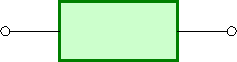
\includegraphics[width=0.7\linewidth]{teo_fig023.pdf}
        \caption{Dvojpól}
        \label{teo:fig023}
      \end{figure}

      Libovolnou část obvodu, která je vyvedena k jedné dvojici svorek, nazýváme 
      \textbf{dvojpólem}; jeho schematické označení je na obr. \ref{teo:fig023}. Veličinu, jež 
      fyzikálně charakterizuje dvojpól, nazýváme jeho parametrem. Dvojpóly, které lze 
      charakterizovat jediným reálným parametrem, nazýváme \textbf{ideálními prvky obvodu} anebo 
      krátce \emph{prvky obvodu}.
      
      Z Maxwellovy teorie plyne, že elektromagnetické vlnění vyvolané elektromagnetickými jevy v 
      obvodu se šíří prostorem rychlostí světla. Pro jednoduchost předpokládejme, že 
      elektromagnetická vlna má harmonický průběh. Jsou-li geometrické rozměry reálného 
      elektrického obvodu zanedbatelně malé ve srovnání s délkou elektromagnetického vlnění, lze 
      rychlost jeho šíření považovat za nekonečně velkou a geometrické rozměry reálného 
      elektrického obvodu se neuplatní — napětí a proudy v tomto obvodu jsou pak pouze funkcí času 
      t. Lze jej modelovat obvodem, jehož magnetické pole je \emph{kvazistacionámi}; parametry jeho 
      dvojpólů nejsou funkcemi geometrických souřadnic. Hovoříme o \emph{obvodu se soustředěnými 
      parametry}.
      
      Nejsou-li geometrické rozměry reálného elektrického obvodu zanedbatelné vzhledem k délce 
      elektromagnetické vlny, je nutné brát v úvahu konečnou rychlost šíření elektromagnetického 
      vlnění — napětí a proudy v tomto obvodu pak budou nejen funkcemi času \(t\), ale též polohy v 
      prostoru, určené souřadnicemi \(x, y, z\) (zpravidla postačí jediná souřadnice). Parametry 
      dvojpólů takového obvodu jsou též funkcemi polohy, a proto hovoříme o \emph{obvodu s 
      rozprostřenými (rozloženými) parametry}.
            
      Teorie obvodů je úzce spjata s kybernetikou, a proto jsou některé pojmy těchto vědních oborů 
      společné. Jak známo, kybernetika se zabývá studiem \emph{systémů libovolné povahy, které jsou 
      schopny přijímat, uschovávat a zpracovávat informaci a využívat ji k řízení}. Obvod je 
      speciálním případem systému, v němž dochází k interakci s okolím na \emph{vstupu (na 
      vstupních svorkách)} a na \emph{výstupu (na výstupních svorkách)}; na vstup jsou připojeny 
      \emph{zdroje energie}, na výstup \emph{spotřebiče}. Napětí a proudy na vstupu představují 
      \emph{podněty (stimuly)} čili \emph{vstupní veličiny}, na výstupu představují \emph{odezvy 
      (reakce)} čili \emph{výstupní veličiny}.
      
      Základními vlastnostmi obvodu jsou: \emph{chování obvodu}, tj. závislost mezi podněty a 
      odezvami a \emph{struktura obvodu}, tj. vlastnosti jeho prvků a způsob jejich spojení. 
      Strukturu obvodu charakterizují jednak fyzikální vlastnosti prvků tvořících obvod, jednak 
      způsob jejich vzájemného spojení. V prvém případě hovoříme o \emph{fyzikální struktuře} 
      obvodu, ve druhém o jeho \emph{topologické (geometrické) struktuře}\cite[s.~21]{Meyer1978}.
      
      
    \subsection{Fyzikální struktura obvodů} 
      \subsubsection{Uzly a větve obvodu, orientace větví, větvové proudy a 
      napětí}\label{TEO:chap_Term}
        Místo styku dvou nebo několika svorek prvků obvodu nazýváme \emph{uzlem obvodu}. Dvojpól 
        spojující dvojici uzlů nazýváme \emph{větví obvodu}. Větve obvodu orientujeme, jestliže 
        jeden z uzlů větve zvolíme za počáteční a druhý za koncový. Větve obvodu lze orientovat 
        libovolně, avšak pro pevně zvolený časový okamžik \(t\). Protože směry proudů ve větvích se 
        mohou s časem měnit, nemusí se v obecném okamžiku \(t\) shodovat orientace větví se směry 
        proudů ve větvích. Pro obvody se soustředěnými parametry a se zavedenou orientací větví 
        definujeme: \emph{Okamžitou hodnotou větvového proudu} \(i\) budeme nazývat okamžitou 
        hodnotu proudu procházejícího průřezem větve, jehož orientace (směr normály) je dána 
        orientací větve. Z této definice plyne, že okamžitá hodnota větvového proudu je kladná v 
        čase \(t\), kdy je směr proudu ve větvi souhlasný s orientací větve a záporná pro ta \(t\), 
        kdy je směr proudu opačný. Okamžitý směr proudu budeme ve schématech vyznačovat šipkou 
%        \begin{tikzpicture}\draw[-open triangle 45] (0,0) -- (1,0);\end{tikzpicture} podle obr. 
        \ref{teo:fig024}.

        \begin{figure}[ht!]  %\ref{teo:fig024}
          \centering
          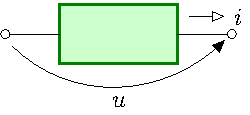
\includegraphics[width=0.7\linewidth]{teo_fig024.pdf}
          \caption{Větvový proud \(i\), větvové napětí \(u\) a orientace větve}
          \label{teo:fig024}
        \end{figure}

        \emph{Okamžitou hodnotou větvového napětí} u budeme nazývat okamžitou hodnotu napětí mezi 
        počátečním a koncovým uzlem orientované větve v daném čase \(t\). Orientaci větvového 
        napětí budeme ve schématech vyznačovat šipkou 
%        \begin{tikzpicture}\draw[-triangle 45] (0,0) to (1,0);\end{tikzpicture} podle obr. 
        \ref{teo:fig024}, přičemž šipka směřuje od počátečního ke koncovému uzlu 
        orientované dráhy, po níž se napětí měří.
        
      \subsubsection{Ideální prvky obvodu a jejich chování}
        Ideální prvky jsou z hlediska svých fyzikálních vlastností i matematického popisu 
        nejjednoduššími dvojpóly obvodu. O vodičích, které je spojují, předpokládáme, že mají 
        nulový odpor a že průchodem proudu nevzniká v jejich okolí magnetické pole. Elektrické 
        pole, jež je obecně vírové, je vně každého prvku obvodu polem potenciálním. Z toho plyne, 
        že hodnota napětí mezi dvojicemi uzlů obvodu nezávisí na tvaru integrační dráhy (tj. na 
        uspořádání přívodů voltmetru) mezi těmito uzly.
        
        Ideální prvky obvodu dělíme na aktivní a pasívní.
        
        \textbf{Aktivní prvky} jsou zdroje elektrické energie (generátory). Zpravidla přijímají 
        neelektrickou formu energie (např. mechanickou, chemickou, tepelnou) a přeměňují ji na 
        elektrickou energii, kterou dodávají do obvodu. Rozlišujeme dva typy aktivních prvků:
        \begin{itemize}
          \item ideální zdroje napětí obr. 5a), jejichž jediným parametrem je svorkové napětí     
                \(u_0 =  u_0(t)\)
          \item ideální zdroje proudu obr. 5b), jejichž jediným parametrem je dodávaný proud      
                \(i_0 = i_0(t)\)
        \end{itemize}
        
        Napětím ideálního napěťového zdroje rozumíme okamžitou hodnotu napětí mezi svorkami zdroje 
        v pořadí, jež stanovíme tím, že první svorku označíme znakem + a druhou znakem —. Svorky 
        zdroje tedy tvoří uspořádanou dvojici: svorka + se bere jako první a svorka — jako druhá. U 
        zdrojů časově proměnného napětí nemusejí znaky + a — představovat skutečnou polaritu 
        svorek; jsou to referenční znaky, jež pouze vyjadřují, že udávané napětí je měřeno od 
        svorky označené + ke svorce označené —. Skutečnou polaritu svorek vyjadřují v těch 
        okamžicích, v nichž je \(u_0(t) > 0\).
        
        V teorii obvodů se ideální zdroje dělí dále na \emph{nezávislé (autonomní)} a na 
        \emph{řízené (závislé, neautonomní)}.
        \begin{itemize}
          \item \textbf{Nezávislý ideální zdroj napětí} má svorkové napětí \(u_0 = u_0(t)\) 
                nezávislé na zatížení zdroje (tj. na výkonu dodávaném zdrojem do obvodu).
          \item \textbf{Nezávislý ideální zdroj proudu} dodává do obvodu proud \(i_0 = i_0(t)\) 
                nezávislý na zatížení zdroje.
          \item \textbf{Řízený ideální zdroj napětí, řízený napětím}, má svorkové napětí, jež je 
                funkcí napětí na některé části obvodu.
          \item \textbf{Řízený ideální zdroj napětí}, řízený proudem, má svorkové napětí, jež je 
                funkcí proudu v některé části obvodu.
          \item \textbf{Řízený ideální zdroj proudu}, řízený napětím, dodává proud, jenž je funkcí 
                napětí v některé části obvodu.
          \item \textbf{Řízený ideální zdroj proudu}, řízený proudem, dodává proud, jenž je funkcí 
                proudu v některé části obvodu.
        \end{itemize}
        
        S řízenými zdroji se často setkáváme v elektronice. Například zesilovač napětí lze nahradit 
        řízeným ideálním zdrojem napětí, přičemž napětí zdroje je funkcí napětí nebo proudu 
        přiváděného na vstup zesilovače.

        \emph{Základních obvodových prvků} je celkem pět: rezistor, cívka, kondenzátor, ideální 
        zdroj napětí, ideální zdroj proudu. Zdůrazněme následující skutečnosti:
        \begin{itemize}
          \itemsep0em 
          \item Každý ze základních prvků je uvažován jako \textbf{ideální} (nemá žádné jiné  
                parazitní vlastnosti).
          \item Kombinací základních prvků vznikne \textbf{náhradní zapojení} skutečného prvku, 
                včetně jeho parazitních vlastností.
          \item Z pěti základních prvků je tedy možno sestavit \textbf{libovolný obvodový model}
                (elektrický obvod) \textbf{pasivní} i \textbf{aktivní}.
          \item U \textbf{aktivních obvodů} (např. zesilovačů) se uplatňují řiditelné, neboli
                parametrické prvky. Typickým příkladem je bipolární tranzistor, jenž je řízen 
                proudem do báze.
        \end{itemize}
      
      \subsubsection{Přizpůsobení zdroje a spotřebiče}
        Zajímavé je sledovat, jak se mění napětí, proud a výkon na spotřebiči v závislosti na 
        poměru odporu spotřebiče a vnitřního odporu zdroje. Jednoduchou úvahou lze usoudit, že 
        největší napětí je naprázdno při nekonečném odporu spotřebiče a největší proud bude při 
        nulovém odporu spotřebiče (zkratu). Maximum výkonu nebude ani při maximálním proudu, 
        protože napětí na zkratu je nulové, ani při maximálním napětí, protože obvodem neprotéká 
        proud. Výkon, který je součinem napětí a proudu, je v obou případech nulový.
        
        Pokud připojíme k náhradnímu napěťovému schématu zdroje spotřebič, bude pro protékající 
        proud platit: \(I = \frac{U_i}{R_i + R_z}\). Po dosazení vztahu pro napětí na spotřebiči, 
        které je shodné se svorkovým napětím zdroje \(U=I\cdot R_z\), získáme vztah: \(U = 
        U_i\frac{R_z}{R_i + R_z}\).
        
  \section{Topologická struktura obvodů}
    Topologické vlastnosti obvodů lze studovat pomocí teorie grafů, jež je odvětvím 
    topologie\footnote{Topologie je moderní	matematická disciplína zabývající se studiem takových 
    vlastností objektů, jež jsou invariantní vzhledem k vzájemně jednoznačnému spojitému zobrazení, 
    jehož inverzní zobrazení je též spojité. Tyto vlastnosti se nazývají topologické vlastnosti 
    (topologické invarianty). (Zmíněné zobrazení lze názorně interpretovat jako takové deformování 
    zkoumaného objektu, při němž se nesmí objekt porušit ani spojovat.) Například hovoříme-li o 
    topologických vlastnostech obvodů, nemáme na mysli způsob rozmístění prvků obvodu v prostoru, 
    nýbrž počet prvků a vlastnosti jejich vzájemného spojení. Studium topologických vlastností 
    obvodů spadá do odvětví topologie, zvaného teorie grafů. Základy teorie grafů byly vybudovány 
    právě na základě potřeb teorie obvodů (G. Kirchhoff).}
    
    \subsection{Základní pojmy z topologie obvodů}
      Definice grafu obvodu. Mějme v prostoru body \(B_1; B_2;\cdots; B_{n_u}\) — nazveme je uzly. 
      Dvojice těchto uzlů nechť tvoří krajní body navzájem se neprotínajících oblouků (tzv. 
      topologických úseček) \(v_1; v_2; \cdots; v_{n_v}\) — nazveme je \emph{větvemi}. Množinu 
      všech větví pak nazýváme \emph{grafem obvodu}.
      
      Graf obvodu tedy vyjadřuje topologickou strukturu obvodu a získáme jej tím, že jej 
      abstrahujeme od fyzikálních vlastností prvků obvodu. U grafu nás nezajímají jeho metrické 
      vlastnosti, tj. uzly grafu lze libovolně rozmístit a jeho větve lze libovolně deformovat, 
      avšak nesmíme je přerušit a po jejich deformaci je popřípadě opět spojit.
      
      Graf, který vznikne z grafu \(\mathscr{G}\) těmito úpravami, nazýváme \emph{izomorfním} (čili 
      \emph{topologicky ekvivalentním}) s grafem \(\mathscr{G}\). Na obr. \ref{TEO:fig_topo01} je 
      příklad obvodu a jeho tří izomorfních grafů.
      
      \begin{figure}[ht!]
        \centering
        \includegraphics[width=0.9\linewidth]{TEO_topo01.jpg}
        \caption{ Obvod (a) a jeho topologicky ekvivalentní (izomorfní) grafy (b), (c), (d) 
                  \cite[s.~39]{Meyer1978}}
        \label{TEO:fig_topo01}
      \end{figure}
      
      Uzly grafu jsou charakterizovány svým stupněm: \emph{stupeň uzlu} \(\varepsilon\) udává počet 
      větví grafu, jež s uvažovaným uzlem \emph{incidují}\footnote{Dva geometrické útvary nazýváme 
      \textbf{incidentní} (resp. říkáme, že spolu incidují), jestliže jeden z nich obsahuje útvar 
      druhý. Například všechny přímky procházející daným bodem jsou s ním incidentní, nebo všechny 
      křivky ležící na ploše s ní incidují.}. Uzel stupně \(0\) (tzv. \emph{izolovaný uzel}) a uzel 
      stupně \(1\) (větev s ním incidující se nazývá \emph{izolovaná}) mají význam v matematické 
      teorii grafů, ale v grafech obvodů se setkáváme jen s uzly stupně \(\varepsilon\geqq 2\). 
      Někdy je výhodné vypustit uzly stupně \(2\) (tzv. vnitřní uzly větví) a uvažovat jen uzly 
      stupně \(\varepsilon\geqq 3\). Tím zmenšíme počet větví obvodu, avšak v jeho větvích obecně 
      nebude již jediný prvek, ale složitější dvojpól — sériové spojení prvků; např. v grafu obvodu 
      na obr. \ref{TEO:fig_topo01} jsou uzly \(B_1; B_2; B_3; B_4\) vesměs 3. stupně, uzly \(B_5; 
      B_6\) jsou 2. stupně vnitřní uzly); graf má \(n_v = 8\) větví. Omezíme-li se na uzly stupně 
      \(\varepsilon\geqq 3\), představují větve \(v_3; v4\) jedinou větev s krajními uzly \(B_2; 
      B_3\) a podobně větve \(v_7; v_6\) tvoří jedinou větev s uzly \(B_2; B_4\) graf má pak jen 
      \(n_v = 6\) větví.
      
      Dvojici grafů, jejichž izomorfismus je porušován jen uzly 2. stupně, nazýváme 
      \emph{homeomorfními}. Homeomorfní grafy jsou tedy takové grafy, jež se po odstraněni 
      některých uzlů 2. stupně stanou izomorfními.
  
  \section{Kirchhoffovy zákony}
    V této kapitole budeme formulovat Kirchhoffovy zákony a ukážeme, jak lze jejich použitím popsat 
    chováni obvodu soustavou rovnic.
    
    \subsection{Formulace prvního a druhého Kirchhoffova zákona}
      Kirchhoffovy zákony, spolu se vztahy mezi napětími a proudy pasivních prvků (tab. 3), mají 
      pro teorii obvodů základní význam. \emph{Platí pro jakýkoliv obvod se soustředěnými 
      parametry}, lineární i nelineární, s parametry časově konstantními i s časově proměnnými. Z 
      hlediska teorie obvodů lze Kirchhoffovy zákony považovat za postuláty, z nichž tato teorie 
      vychází. Z hlediska teorie elektromagnetického pole jsou však důsledkem plynoucím z 
      Maxwellovy teorie.
      
%     \begin{mdframed}[style=MyFrame]
      \textbf{První Kirchhoffův zákon}. Pro libovolný uzel obvodu platí: Součet okamžitých hodnot 
      proudů vystupujících z uzlu a proudů vstupujících do uzlu je roven nule. Přitom proudy 
      vystupující z uzlu bereme jako kladné a proudy vstupující do uzlu jako záporné.
%     \end{mdframed} 
      
      \begin{proof}
        Uvažujme libovolný uzel obvodu \(B_j\). Obklopíme jej libovolnou uzavřenou orientovanou 
        plochou \(S\) obr. \ref{TEO:fig_KZ01}a). Vzhledem k tomu, že magnetické pole obvodu se 
        soustředěnými parametry je kvazistacionární, má rovnice kontinuity tvar
        \begin{equation}
          \oint_s \vec{J}(t)\dd{\vec{S}} = 0
        \end{equation}
        \begin{figure}[ht!]
          \centering
          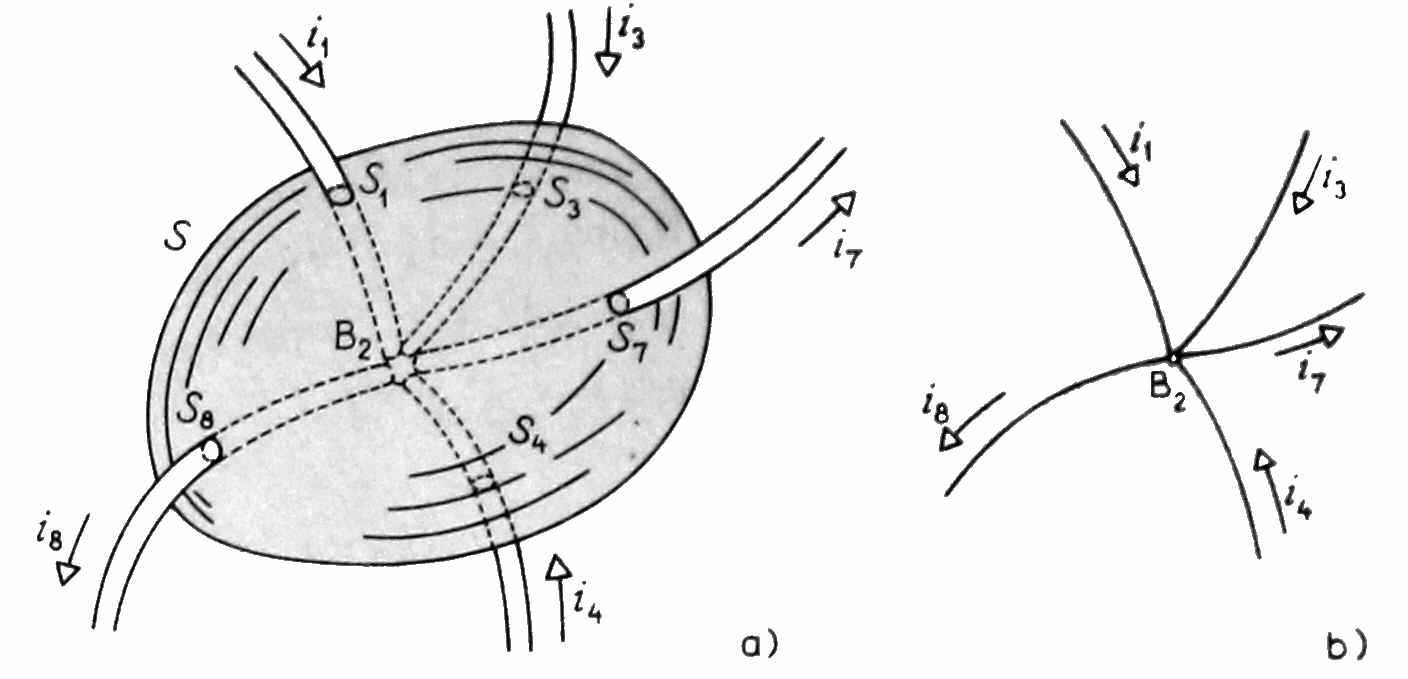
\includegraphics[width=0.9\linewidth]{TEO_KZ01.jpg}
          \caption{Uzel incidující s pěti větvemi: reálný elektrický obvod (a) a ideální obvod (b). 
                   (K odvozeni prvního Kirchhoffova zákona) \cite[s.~47]{Meyer1978}}
          \label{TEO:fig_KZ01}
        \end{figure}      
        Pro tok vektoru proudové hustoty uzavřenou plochou \(S\) podle obr. \ref{TEO:fig_KZ01}a) 
        platí
        \begin{equation}
          \oint_s \vec{J}(t)\dd{\vec{S}} = \sum_{\mathclap{\substack{k\\B_j\in v_k}}}
                                           \int_{S_k} \vec{J}(t)\dd{\vec{S}} 
        \end{equation}
        kde sumace na pravé straně rovnice je provedena přes indexy všech větví incidujících s 
        uzlem \(B_j\). Jednotliví sčítanci představují proudy vystupující z uzlu, resp. vstupující 
        do uzlu. Porovnáním obou uvedených vztahů plyne dokazovaný první Kirchhoffův zákon.
      \end{proof}
      
      Matematicky lze zapsat první Kirchhoffův zákon pro libovolný uzel obvodu \(B_j\) pomocí 
      větvových proudů \(i_k\) libovolně orientovaných větví \(v_k\)\footnote{Orientace větví 
      obvodu je libovolná, ale pevně zvolená (nezávislá na čase), viz kap. \ref{TEO:chap_Term}.} ve 
      tvaru 
      \cite[s.~47]{Meyer1978}
      \begin{equation}\label{TEO:eq_KZI}
        \sum_{\mathclap{\substack{k\\B_j\in v_k}}} \pm i_k = 0; \qquad j = 1;\ldots; n_u 
      \end{equation}
      Znaménko \(+\) platí, je-li větev \(v_k\) orientována tak, že uzel \(B_j\) je jejím 
      počátečním uzlem a znaménko \(—\) platí v opačném případě; sčítáme pro všechna \(k\), pro něž 
      uzel \(B_j\) inciduje s větví \(v_k (B_j\in v_k)\); \(n_u\) je počet všech uzlů obvodu. 
      Poznamenejme, že podle definice větvového proudu (viz kap. \ref{TEO:chap_Term}) je \(i_k > 
      0\), souhlasí-li směr proudu s orientaci větve a \(i_k < 0\) v opačném případě.
      
      Například pro uzel \(B_2\) podle obr. \ref{TEO:fig_KZ01}b) má první Kirchhoffův zákon tvar
      \begin{equation*}
        -i_1 - i_3 - i_4 + i_7 + i_8 = 0
      \end{equation*}
      Rovnice (\ref{TEO:eq_KZI}) je symbolickým zápisem prvního Kirchhoffova zákona, vyžadujícím 
      slovní komentář o tom, kdy máme brát znaménko \(+\) , kdy znaménko \(—\) a jakých hodnot 
      nabývá sčítací index \(k\). Tento zápis prvního Kirchhoffova zákona je velmi dobře použitelný 
      pro řešení jednodušších obvodů. Naproti tomu při řešení obvodů na počítači je třeba vyjádřit 
      první Kirchhoffův zákon výstižnějším zápisem ve tvaru
      \begin{equation}\label{TEO:eq_KZI_01}
        \sum\limits_{k=1}^{n_v} a_{jk} i_k = 0; \qquad j = 1;\ldots; n_u 
      \end{equation}
      \begin{figure}[ht!]
        \centering
        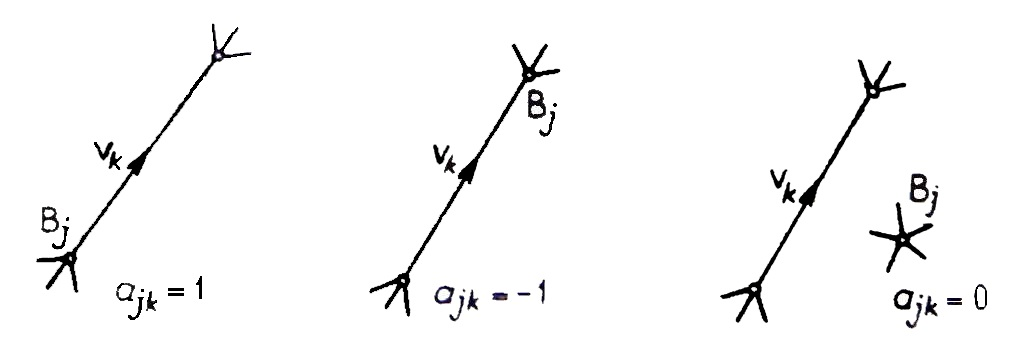
\includegraphics[width=0.9\linewidth]{TEO_KZ02.jpg}
        \caption{K určení hodnot koeficientů \(a_{jk}\) \cite[s.~47]{Meyer1978}}
        \label{TEO:fig_KZ02}
      \end{figure}
      kde koeficienty \(a_{jk}\) vyjadřují incidenci uzlů a větví v orientovaném grafu obvodu a 
      nabývají těchto hodnot: \(a_{jk} = 1\), když j-tý uzel je počátečním uzlem k-té větve, 
      \(a_{jk} = — 1\), když j-tý uzel je koncovým uzlem k-té větve a \(a_{jk} = 0\), když j-tý 
      uzel neinciduje s k-tou větví (obr. \ref{TEO:fig_KZ02}). Znaménko větvového proudu \(i_k\) 
      plyne ze souhlasnosti, resp. nesouhlasnosti orientace větve a směru větvového proudu (\(i_k > 
      0\), resp. \(i_k < 0\)).
      
      \textbf{Druhý Kirchhoffů v zákon}. Pro libovolnou orientovanou smyčku obvodu platí: Součet 
      okamžitých hodnot napětí na všech větvích incidujících s orientovanou smyčkou obvodu je roven 
      nule. Přitom napětí větví bereme jako kladná, jestliže proud ve větvi v daném okamžiku 
      prochází ve smyslu orientace smyčky a jako záporná, jestliže prochází v opačném směru.
      
      \begin{proof}
        Uvažujme libovolnou orientovanou uzavřenou křivku \(s_j\) procházející všemi uzly smyčky 
        obvodu a vedenou vně prvků (např. křivku vyznačenou na obr. \ref{TEO:fig_KZ03} tečkovaní). 
        Z vlastností ideálních prvků obvodu plyne, že II. Maxwellova rovnice v integrálním tvaru má 
        pro křivku \(s_j\) tvar
        \begin{align}
          \oint\vec{E}\dd{\vec{l}} &= 0    \label{TEO:eq_KZ01} \\
          \shortintertext{Pro oběhové napětí po křivce \(s_j\) (obr. \ref{TEO:fig_KZ03}) zároveň 
                          platí vztah}
          \oint\vec{E}\dd{\vec{l}} &= \sum_{\mathclap{\substack{k\\v_k\in s_j}}}\vec{E}\dd{\vec{l}}
        \end{align}
        Porovnáním obou uvedených vztahů plyne dokazovaný druhý Kirchhoffův zákon.
        \begin{figure}[ht!]
          \centering
          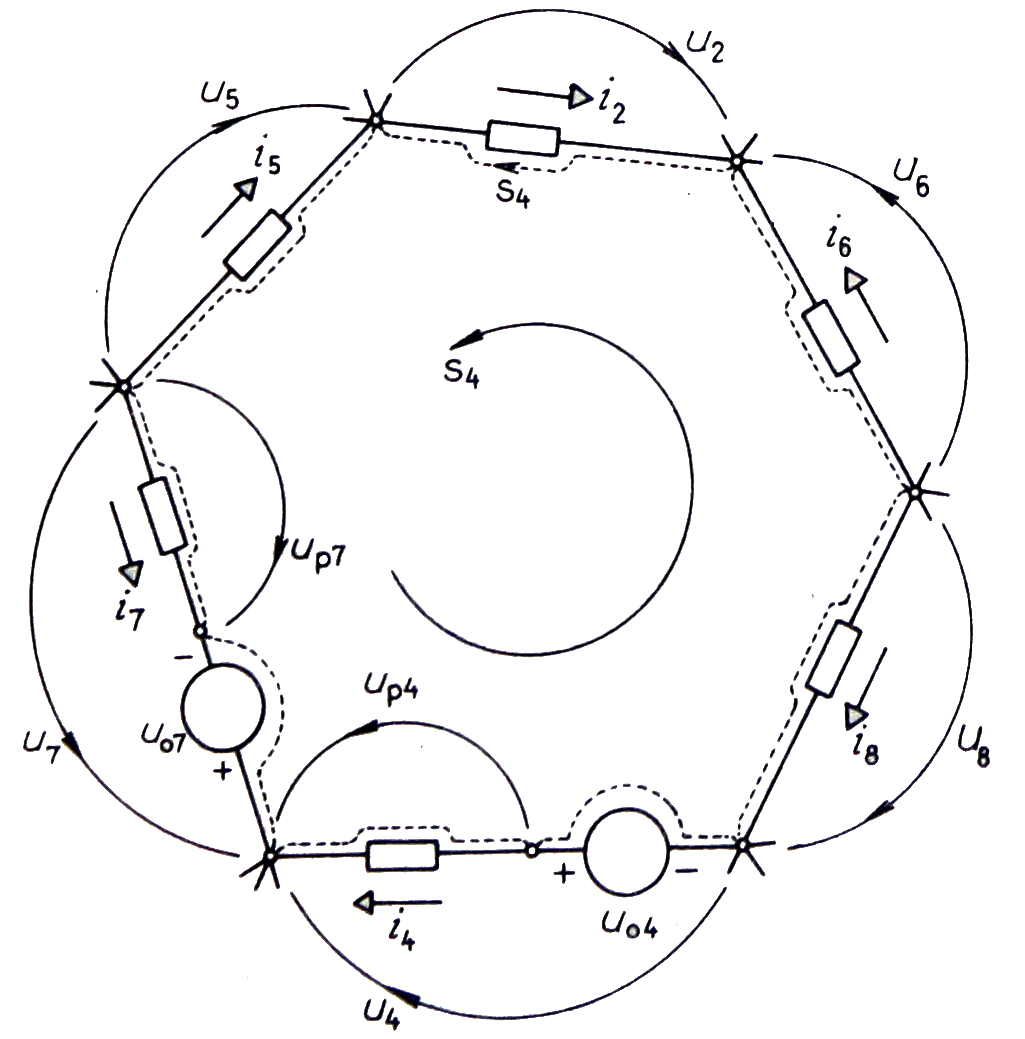
\includegraphics[width=0.7\linewidth]{TEO_KZ03.jpg}
          \caption{Smyčka incidující se šesti větvemi (K odvození druhého Kirchhoffova 
                   zákona)\cite[s.~48]{Meyer1978}}
          \label{TEO:fig_KZ03}
        \end{figure}
      \end{proof}
      Matematicky lze vyjádřit druhý Kirchhoffův zákon pro libovolnou orientovanou smyčku \(s_j\) 
      pomocí větvových napětí \(u_k\) libovolně orientovaných větví \(v_k\) ve tvaru
      \begin{equation}\label{TEO:eq_KZ03}
        \sum_{\mathclap{\substack{k\\v_k\in s_j}}} \pm u_k = 0 \qquad j=1;\cdots; n_s
      \end{equation}
      Znaménko \(+\) platí, je-li větev \(v_k\) orientována souhlasně se smyčkou \(s_j\) a znaménko 
      \(—\) platí v opačném případě; sčítáme pro všechna \(k\), pro něž větev \(v_k\) inciduje se 
      smyčkou \(s_j (v_k\in s_j)\); \(n_s\) je počet všech smyček obvodu.
      
      Například pro smyčku \(s_4\) podle obr. \ref{TEO:fig_KZ03} má druhý Kirchhoffův zákon tvar
      \begin{equation*}
        -u_2 -u_4 -u_5 +u_6 +u_7 -u_8 = 0
      \end{equation*}
      
      Vyjádření druhého Kirchhoffova zákona rovnicí (\ref{TEO:eq_KZ03}) je — obdobně jako vyjádření 
      prvního Kirchhoffova zákona rovnicí (\ref{TEO:eq_KZI}) — jen symbolickým zápisem, k němuž 
      bylo nutno připojit slovní komentář. Pro řešení obvodů na počítači je třeba vyjádřit druhý 
      Kirchhoffův zákon matematicky výstižnějším zápisem
      \begin{equation}\label{TEO:eq_KZ04}
        \sum\limits_{k=1}^{n_v} b_{jk} u_k = 0 \qquad j=1;\cdots; n_s
      \end{equation}      
      \begin{figure}[ht!]
        \centering
        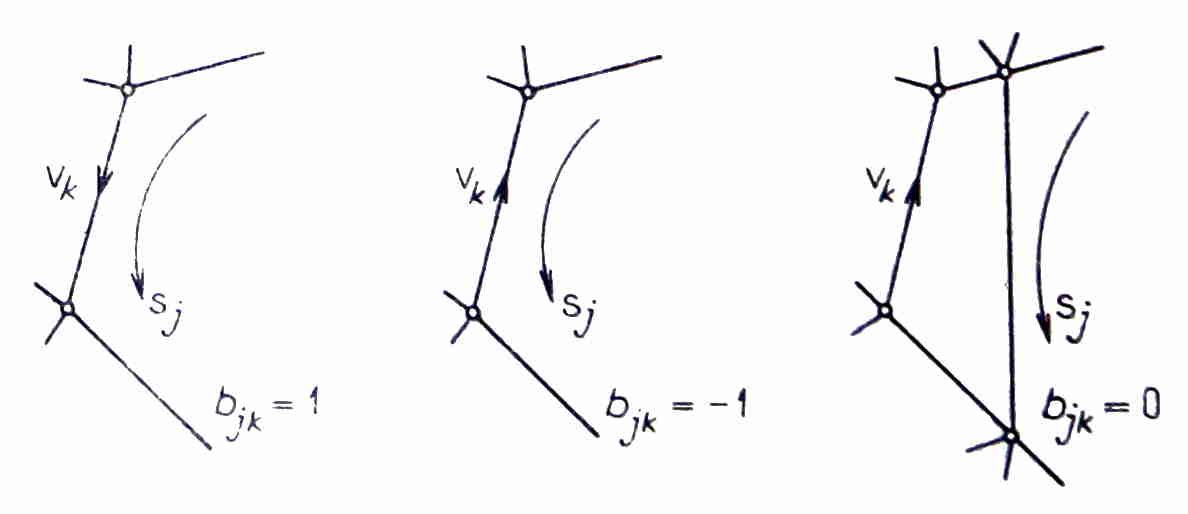
\includegraphics[width=0.9\linewidth]{TEO_KZ04.jpg}
        \caption{K určení koeficientů \(b_{jk}\) \cite[s.~49]{Meyer1978}}
        \label{TEO:fig_KZ04}
      \end{figure}      
      kde koeficienty \(b_{jk}\) vyjadřují incidenci smyček a větví v orientovaném grafu obvodu a 
      nabývají těchto hodnot: \(b_{jk} = 1\), když \(k\)-tá větev inciduje s \(j\)-tou smyčkou a 
      orientace obou se shodují, \(b_{jk} = — 1\), když \(k\)-tá větev inciduje s \(j\)-tou smyčkou 
      a orientace obou je opačná, a \(b_{jk} = 0\), když \(k\)-tá větev neinciduje s \(j\)-tou 
      smyčkou (obr. \ref{TEO:fig_KZ04}).
      
  \section{Analýza elektrických obvodů}
    Pojem \textbf{analýza} není v teorii elektrických obvodů používán v původním širokém smyslu. 
    Zejména v souvislosti s počítačovým řešením obvodů se pod analýzou obvykle rozumí 
    \emph{konkrétní metody získávání elektrických charakteristik obvodů z jejich modelů} (například 
    kmitočtová nebo stejnosměrná analýza).
    
    \subsection{Modelování, analýza, simulace}
      \emph{Analýzu} provádíme ve snaze získat informace o určitých vlastnostech zkoumaného obvodu, 
      které nás zajímají. Z praktických důvodů však zpravidla analýze nepodrobujeme samotný obvod, 
      nýbrž jeho \emph{model}. Jedním z dobrých důvodů může být skutečnost, že daný obvod dosud 
      existuje pouze v představě návrháře a před jeho výrobou je vhodné ověřit, zda je navržen 
      správně. K modelování obvodu máme k dispozici elementární modely elektrických prvků (pasivní 
      R, L, C, tranzistory, operační zesilovače apod.) ve formě matematického popisu jejich 
      fungování a  jejich elektrotechnických značek, které jsou začleněny do schématu celkového 
      zapojení. Z hlediska matematického je model obvodu představován soustavou rovnic, které lze 
      odvodit na základě rovnic dílčích elektrických prvků a Kirchhoffových rovnic, které 
      reprezentují způsob propojení součástek \cite[s.~16]{Biolek}.
      
      Při modelování obvodu je důležité nejprve uvážit, s jak složitým modelem bude vhodné 
      pracovat. Složité modely obvykle umožňují věrnější popis chování skutečného obvodu, avšak 
      současně prudce rostou požadavky na výkon analyzačního nástroje. Je zřejmé, že výpočty, které 
      provádíme jen pomocí papíru a tužky, případně kalkulačky, jsou vhodné pro analýzu méně 
      rozsáhlých obvodů s jednoduchými modely, kde nám jde buď o ověření správnosti základního 
      principu fungování, nebo o odhady chování obvodu s odhlédnutím od různých parazitních jevů a 
      vlivů reálných vlastností součástek na vlastnosti obvodu. Složité modely si můžeme dovolit 
      používat při analýze s využitím speciálních počítačových programů.

      Klasická teorie obvodů dává odpověď na otázku, s jakým minimálním počtem typů elementárních 
      modelů obvodových prvků je možné sestavit model jakkoliv složitého analogového obvodu se 
      soustředěnými parametry: jsou to pasivní prvky typu R,L,C a zdroje klasické a řízené. 
      Příslušné charakteristiky těchto prvků jsou popsány jednoduchými nebo složitými rovnicemi. Z 
      tohoto pohledu můžeme říci, že k sestavování modelů daných obvodů a k jejich využívání nemáme 
      k dispozici nic jiného než omezený počet modelů elementárních prvků s příslušnými 
      matematickými vzorci \cite[s.~17]{Biolek}.
      
      Od jisté úrovně modelování, která zajišťuje uspokojivou shodu chování modelu a originálu, je 
      možné model využívat k simulaci skutečného chování obvodu za konkrétních podmínek. Příkladem 
      může být sledování vlivu teploty na nastavený stejnosměrný pracovní bod tranzistorového 
      zesilovače. Dostáváme se k poslednímu pojmu z trojlístku \emph{modelování - analýza - 
      simulace}. Simulace je tedy něco více než analýza (v úzkém pojetí) a analýza je důležitá 
      součást simulace.
      
      \begin{figure}[ht!]
        \centering
        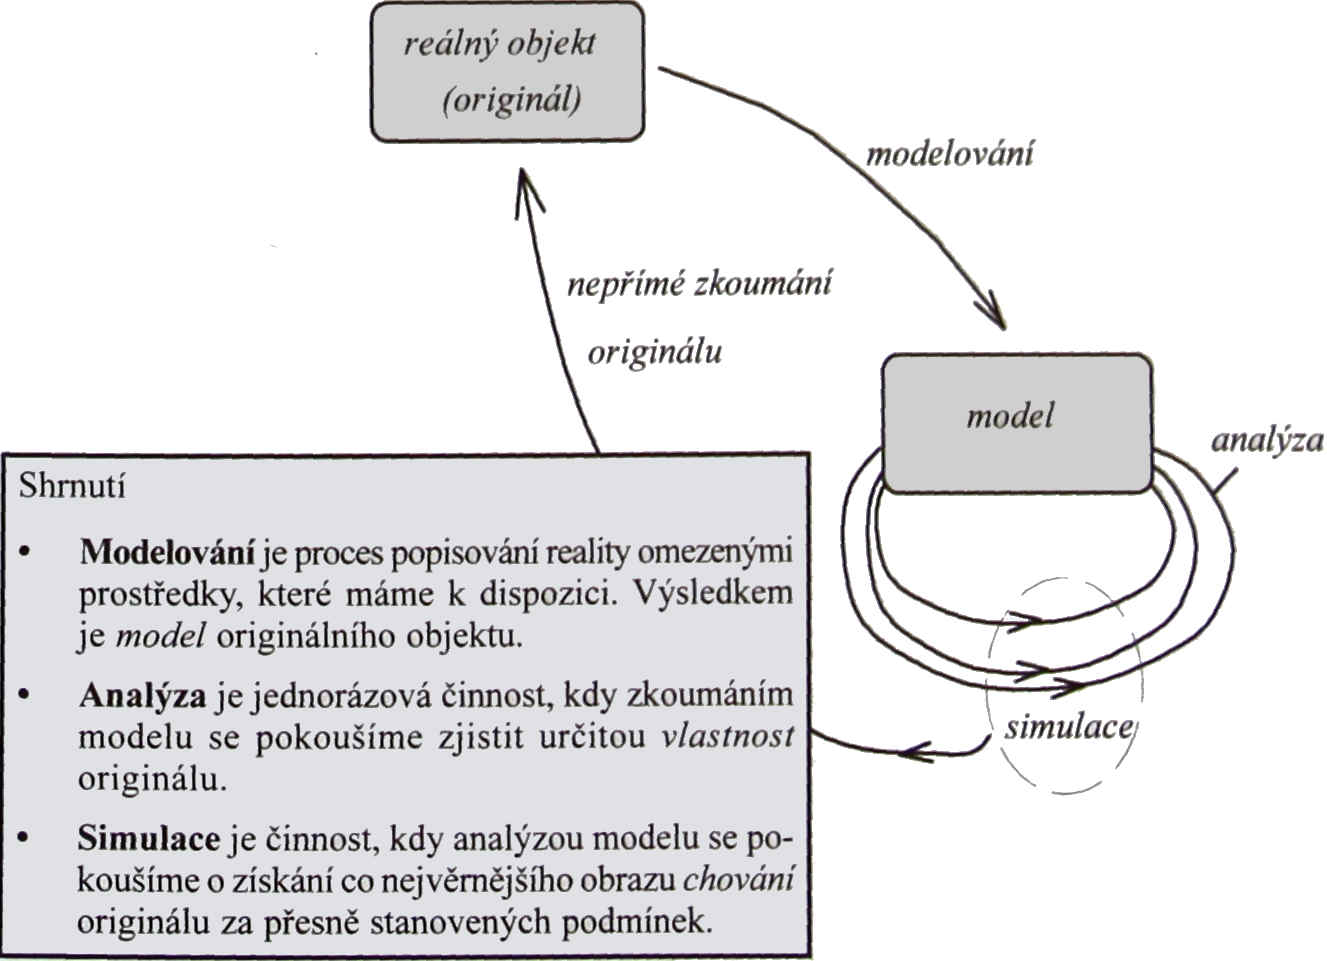
\includegraphics[width=0.95\linewidth]{Biolek_Modelovani.jpg}
        \caption{Modelováni, analýza, simulace \cite[s.~17]{Biolek}}
        \label{TEO:fig_modelovani}
      \end{figure}
      
      Shrnutí:
      \begin{itemize}
        \itemsep0em
        \item \emph{Při řešení obvodu pomocí „papíru, tužky a kalkulačky“} nejprve sestavíme model 
              obvodu ve formě schématu zapojení včetně parametrů, resp. charakteristik jednotlivých 
              součástek. Z tohoto modelu pak vzniká model matematický ve formě rovnic, které 
              vyplývají z vzájemného propojení a vlastností součástek, Kirchhoffových zákonů a 
              Ohmová zákona. Tento model pak podrobíme numerické analýze.      
        \item \emph{Při řešení pomocí počítačového programu} opět sestavujeme model obvodu,  
              většinou pomocí schematického editoru. Program je však schopen při tomto sestavování 
              účinně pomáhat tím, že je zdrojem složitých interních modelů součástek (tranzistory, 
              operační zesilovače, integrované obvody...). Vlastní sestavení rovnic, jejich řešení 
              a vizualizace výsledků je již plně v režii programu \cite[s.~18]{Biolek}.
      \end{itemize}
      
    \subsection{Metody analýzy heuristické a algoritmické}
      Metodu analýzy můžeme chápat jako konkrétní postup od modelu obvodu až po získání cíle analýzy.
      
      Všechny existující metody analýzy můžeme rozdělit na \emph{nealgoritmické (heuristické)} a 
      \emph{algoritmické}. Do první kategorie patří postupy, které řešitel volí na základě svých 
      předchozích zkušeností s využíváním tvůrčího přístupu. Například při výpočtu napětí na 
      výstupu zatíženého děliče napětí je možno nejprve sloučením zatěžovacího a pracovního 
      rezistoru převést řešení na problém děliče nezatíženého, posléze vypočítat proud děličem a 
      následně výstupní napětí. Jiným možným postupem je využití Théveninovy věty apod. 
      Algoritmická metoda oproti tomu definuje přesný postup — algoritmus, který vždy vede k cíli. 
      Výše uvedená úloha zatíženého děliče může být řešena například algoritmickou metodou 
      smyčkových proudů.
      
      Zjednodušené řečeno, heuristické metody jsou vhodné k ručnímu řešení méně rozsáhlých obvodů, 
      pokud jsme zběhlejší v elektrotechnických výpočtech a nechybí nám schopnost hledání vlastních 
      cest k cíli.
      
      Při analýze obvodů bez počítačové podpory bychom měli upřednostňovat nealgoritmické metody. 
      Pouze tam, kde je vyjadřování napěťových a proudových poměrů komplikované, např. v důsledku 
      působení speciálních obvodových prvků, je často rozumné úlohu vyřešit \emph{modifikovanou 
      metodou uzlových napětí} (část \ref{TEO:chap_MMUN}) nebo \emph{Masonovým-Coatesovým grafem} 
      (část 2.4). Každá z metod má svůj význam: nealgoritmická nutí k fyzikálnímu myšlení a k 
      pochopení funkce obvodu, který analyzujeme, algoritmická pak poskytuje účinný nástroj k 
      praktickému řešení.

  \section{Metody analýzy elektrických ob\-vo\-dů}
    \subsection{Klasická metoda uzlových napětí (MUN)}
      Metoda uzlových napětí je založena na tomto postupu:
      \begin{itemize}
       \item Jeden z uzlů obvodu se prohlásí za tzv. \textbf{referenční uzel}. Přiřadí se mu 
             číslo 0, případně v počítačovém simulátoru značka uzemnění. Vzhledem k tomuto uzlu se 
             budou vztahovat napětí ostatních uzlů obvodu. Tato napětí se nazývají \textbf{uzlová 
             napětí} a tvoří \textbf{soustavu neznámých obvodových veličin} metody. Je vhodné 
             orientovat všechna uzlová napětí tak, aby čítací šipky směřovaly do referenčního uzlu. 
             Uzlová napětí jsou neznámými metody i tehdy, je-li našim konečným cílem počítat 
             jiné obvodové veličiny. Každé napětí a každý proud v obvodu jsou totiž vyjádřitelné 
             jako lineární kombinace uzlových napětí.
       \item Pro každý uzel obvodu, vyjma referenčního, sestavíme rovnici 1. KZ ve tvaru:
             \emph{součet proudů tekoucích dovnitř uzlu z vnějších zdrojů proudu  = součtu proudů
             vytékajících větvemi obvodu ven z uzlu.}
       \item Rovnice vyřešíme, tj. získáme velikosti uzlových napětí. Z nich pak dopočteme  
             požadovaný výsledek analýzy.
      \end{itemize}
      
      Metodu uzlových napětí lze objasnit na příkladu zapojení na obr. \ref{teo:fig025}. Je
      třeba určit proud $I_{x2}$ 
      \begin{figure}[ht!]  %\ref{teo:fig025}
        \centering
        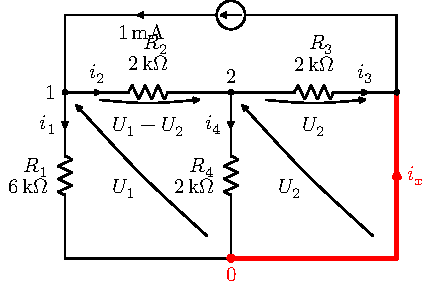
\includegraphics[width=0.7\linewidth]{teo_fig025.pdf}
        \caption{Řešení obvodu metodu uzlových napětí - MUN \cite[s.~62]{Biolek}}
        \label{teo:fig025}
      \end{figure}
      Nejprve očíslujeme uzly. Zvolíme referenční uzel a přiřadíme mu číslo 0. Zde je třeba  
      zdůraznit, že referenční uzel je možno volit zcela libovolně. Většinou se volí tak, aby 
      případné hledané napětí bylo rovno jednomu z napětí uzlových. Dále si všimneme, že uzel, v 
      němž je se spojuje rezistor $R_3$ a proudový zdroj, je vlastně součástí referenčního uzlu a 
      jako takový se přídavně nečísluje - má již označení \num{0}.
      
      Vyznačená uzlová napětí $U_1$ a $U_2$ tvoří soustavu dvou neznámých, k níž musíme sestavit 
      dvě rovnice. Budou to rovnice 1. KZ pro uzly 1 a 2. Protože počítáme proud $I_{x2}$, postačí 
      určit uzlové napětí $U_2$. Z něj totiž snadno určíme proud rezistorem $R_3$ a z něj $I_{x2}$.
      
      Podle obr. \ref{teo:fig025} napíšeme 1. KZ pro rovnováhu proudů v uzlech 1 a 2:
      \begin{align*}
        \text{uzel 1:} \qquad I &=  I_{R1} + I_{R2}            \\
        \text{uzel 2:} \qquad 0 &= -I_{R1} + I_{R2} + I_{R4}  
      \end{align*}
      
      Orientaci čítacích šipek větvových proudů můžeme volit naprosto libovolně. Pokud se v 
      orientaci zmýlíme, vyjde u daného proudu opačné znaménko.
      
      Větvové proudy na pravé straně rovnic vyjádříme pomocí větvových vodivostí a větvových 
      napětí, která závisí na uzlových napětí (viz obr. \ref{teo:fig025}):
      \begin{align}
       \text{uzel 1:} \qquad I &=  G_1U_1 + G_2(U_1-U_2)             \nonumber              \\ 
       \text{uzel 2:} \qquad 0 &= -G_2(U_1-U_2) + G_3U_2 + G_4U_2    \nonumber              \\
       \shortintertext{Vytknutím neznámých upravíme rovnice na konečný tvar}
       \text{uzel 1:} \qquad I &=  (G_1 + G_2)U_1 - G_2U_2           \label{TEO:eq_MUN_pr}  \\ 
       \text{uzel 2:} \qquad 0 &= -G_2U_1 + (G_2 + G_3 + G_4)U_2     \nonumber
       \shortintertext{Dosadíme-li vodivosti v [mS], vyjdou proudy na levé straně v [mA]}
       \text{uzel 1:} \qquad 1 &=  \frac{2}{3}U_1 - \frac{1}{2}U_2   \nonumber              \\ 
       \text{uzel 2:} \qquad 0 &= -\frac{1}{2}U_1 + \frac{3}{2}U_2   \nonumber
       \shortintertext{Tyto rovnice dávají řešení}
                   [U_1, U_2]  &= \left[2, \frac{2}{3}\right] \text{V}  \label{TEO:eq_MUN_vysl}
      \end{align}
      Pohledem na schéma \ref{teo:fig025} zjistíme, že při $U_2 = \frac{2}{3}V$ bude proud 
      $I_{R3} = \frac{1}{3} mA$ a hledaný proud $I_{x2}$ vychází z 1. KZ
      \begin{equation}\label{TEO:eq_MUN_Ix2}
        I_{x2} = I - I_{R3} = \left(1 - \frac{1}{3}\right) = \frac{2}{3} mA.
      \end{equation}

      \subsubsection{Pravidla pro sestavování rovnic}
        Nyní pusťme se do zobecnění poznatků z předchozího příkladu. Rovnice \ref{TEO:eq_MUN_pr} 
        zapíšeme v maticovém tvaru
        \begin{table}[ht!]
          % using \usepackage{array} and command \newcolumntype{C}[1]{>{\centering}m{#1}}!
          \centering
          \begin{tabular}{c|c|c|c|c|c|c|}
             \multicolumn{1}{c}{}      & \multicolumn{1}{c}{}      & \multicolumn{1}{c}{} & 
             \multicolumn{1}{c}{$U_1$} & \multicolumn{1}{c}{$U_2$} & \multicolumn{1}{c}{} & 
             \multicolumn{1}{c}{}              \\
             \cline{2-2} \cline{4-5} \cline{7-7}
              uzel 1:  & $I$   & \multirow{2}{*}{=} & $G_1+G_2$ & $-G_2$         &   & $U_2$    \\
             \cline{2-2} \cline{4-5} \cline{7-7}
              uzel 2:  &       &                    & $-G_2$    & $G_2+G_3+G_4$  &   & $U_2$    \\
             \cline{2-2} \cline{4-5} \cline{7-7}
          \end{tabular}
          \caption*{ }
        \end{table}
        Porovnáme-li maticovou rovnici s původním schématem obvodu \ref{teo:fig025} 
        dospějeme k následujícím pravidlům:
        \begin{itemize}
         \item Pravidlo o sestavení vektoru budicích proudů na levé straně maticové rovnice:
           \begin{itemize}
             \item V $\text{i-tém}$ řádku je algebraický součet proudů, tekoucích dovnitř  
                   $\text{i-tého}$ uzlu z vnějších zdrojů proudu.
           \end{itemize}
         \item Pravidla o sestavení čtvercové vodivostní (admitanční) matice:
           \begin{itemize}
             \item Prvek $i, j$ na hlavní diagonále obsahuje součet všech vodivostí (admitancí),  
                   které jsou připojeny k uzlu $i$.
             \item Prvek $i, j (i \neq j)$ mimo hlavní diagonálu obsahuje záporně vzatý součet všech 
                   vodivostí, které jsou připojeny bezprostředně mezi uzly $i$ a $j$.
           \end{itemize}
        \end{itemize}
        Základní lineární dvojpóly (R, L, C) jsou reciprocitní, tzn. chovají se stejně ve směru 
        obou uzlů. Jinými slovy, jejich impedance je v obou případech stejná. Proto u obvodů s 
        těmito součástkami vykazují admitanční matice \emph{symetrii}, tj. prvky matice \emph{i, j} 
        a \emph{j, i} jsou totožné.

    \subsection{Modifikovaná metoda uzlových napětí}\label{TEO:chap_MMUN}
      Výhodou metody uzlových napětí je její snadná algoritmizace: algoritmus pro sestavení 
      soustavy rovnic přímo ze schématu je velmi jednoduchý a lze jej tedy implementovat do 
      počítačových programů pro analýzu a simulaci. Nevýhodou metody ovšem je, že neumožňuje 
      analyzovat obvody se zdroji napětí a součástkami, které nemají admitanční rovnici. Bohužel, k 
      těmto součástkám patří nejen například takové prvky jako je obyčejný transformátor, ale i 
      různé operační zesilovače, konvejory, a další moderní analogové prvky \cite[s.~77]{Biolek}.
      
      Proto klasická metoda MUN musí být podrobena určité modifikaci, která jednak zachová její 
      výhodu - snadnou algoritmizovatelnost - jednak umožní analyzovat lineární obvody bez výše 
      uvedených omezení. Jsou to metody:
      \begin{itemize}\itemsep0em
        \item Metoda razítek
        \item Metoda zakázaného řádku
        \item Metoda U/I
      \end{itemize}

      \subsubsection{Metoda razítek}
        Každý "problémový" prvek je popsán minimálně jednou přídavnou rovnicí a o stejný počet 
        obohatí množinu neznámých. Současně dojde k modifikaci některých původních rovnic 1. KZ. 
        Maticová rovnice pak získá zvláštní strukturu: k původní admitanční matici MUN přibudou 
        řádky a sloupce, jejichž prvky obecně nemají rozměr admitancí. Jsou to tzv. \emph{razítka} 
        přídavných elektrických prvků. Celá matice se pak nazývá \textbf{pseudoadmitanční}. 
        Zvětšení rozměru soustavy rovnic obvykle při počítačové analýze nemusí být na závadu. Při 
        ručním řešení jde však prakticky vždy o problém \cite[s.~78]{Biolek}.
        
        Uvažujme obvod popsaný rovnicemi klasické MUN. Mezi uzly \emph{a} a \emph{b} obvodu 
        dodatečně připojíme obecný dvojpól, který je popsán svým Théveninovým modelem podle obr. 
        \ref{TEO:fig_MMUN_thev_dvojpol}. Včleněním dvojpólu dojde ke změně napěťových a proudových 
        poměrů v obvodu. Dvojpólem bude protékat proud $I_x$, který modifikuje proudové poměry mezi 
        v uzlech \emph{a} a \emph{b}. Dojde i k změně původních uzlových napětí.
        
        \begin{figure}[ht!]
          \centering
          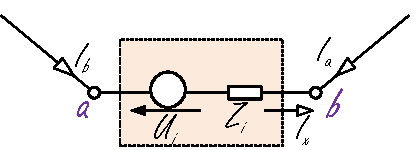
\includegraphics[width=0.7\linewidth]{Biolek_MMUN_thev_dvojpol.pdf}
          \caption[MMUN - Théveninův model dvojpólu]{Začlenění obecného lineárního dvojpólu, 
                   popsaného Théveninovým modelem do obvodu \cite[s.~78]{Biolek}}
          \label{TEO:fig_MMUN_thev_dvojpol}
        \end{figure}
        
        Původní rovnice popisující rovnováhu proudů v uzlu \emph{a} musí být na pravé straně 
        doplněna o proud $I_x$, vytékající ven z uzlu, a v uzlu \emph{b} o proud $I_x$ se záporným 
        znaménkem, protože vtéká dovnitř uzlu \emph{b}. Navíc uzlová napětí $U_a$ a $U_b$ jsou nyní 
        vázána podmínkou
        
        \begin{equation}\label{TEO:eq_MMUN_dvojpol}
          Z_iI_x + U_b = U_i + U_a, \quad\text{neboli}\quad U_i = Z_iI_x + U_b - U_a
        \end{equation}
        Všechny tyto modifikace lze zahrnout do nové soustavy rovnic MMUN:
        
        \begin{figure}[ht!]
          \centering
          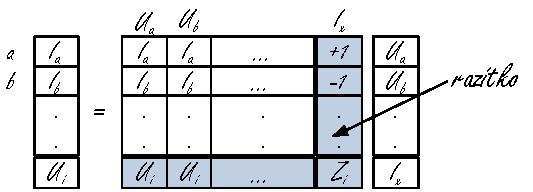
\includegraphics[width=1\linewidth]{Biolek_MMUN_razitko.pdf}
          \caption[MMUN - razítko]{ Razítko v pseudoadmitanční matici \cite[s.~79]{Biolek}}
          \label{TEO:fig_MMUN_razitko}
        \end{figure}
        
        Vektor neznámých uzlových napětí je rozšířen o další neznámou, $I_x$. Počet rovnic je 
        rovněž zvětšen o jedničku, a to o výše uvedenou podmínku mezi uzlovými napětími $U_a$ a 
        $U_b$. Přitom napětí $U_i$ je začleněno do vektoru známých budicích veličin na levé straně. 
        Modifikace rovnic 1. KZ pro uzly \emph{a} a \emph{b} je provedena zápisem $+1$ a $-1$ do 
        sloupce "$I_x$".
        
        Právě provedený zápis je návodem, jak pomocí MMUN analyzovat například obvody obsahující 
        zdroj napětí. Impedance $Z_i$ může být i nulová, pak se bude jednat o ideální zdroj napětí. 
        Při $U_i = 0$ a $I_i = 0$ lze modelovat zkrat mezi uzly a počítat proud, tekoucí tímto 
        zkratem. Toho lze využít například při analýze obvodů s proudem řízenými zdroji. 
        
        V případě, že se v obvodu nachází více prvků bez admitančního popisu, odpovídá každému z 
        nich samostatné razítko. Pseudoadmitanční matice pak nabývá na rozměrech. Metodu budeme 
        blíže konkretizovat na několika příkladech. 
  
        \subsubsection{Pasivní obvody obsahující zdroje napětí a proudu}
          Pomocí MMUN vyřešme zadání z obr. \ref{teo:fig026}. Je hledán proud \(I_x\) 
          vytékající ze zdroje napětí 
          \begin{figure}[ht!]  %\ref{teo:fig026}
            \centering
            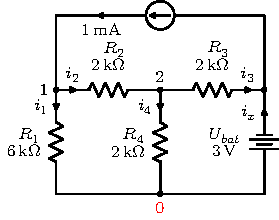
\includegraphics[width=0.7\linewidth]{teo_fig026.pdf}
            \caption{Analyzovaný obvod}
            \label{teo:fig026}
          \end{figure}
          
        \subsubsection{Obvody s ideálním operačním zesilovačem ty\-pu VFA}
          Ideální OPAMP, na obr. \ref{TEO:fig_MMUN_ideal_VFA} po vložení do obvodu způsobí 
          ztotožnění uzlových napětí $U_a$ a $U_b$, a modifikaci proudových poměrů v uzlu \emph{c}.
      
          \begin{figure}[ht!]
            \centering
            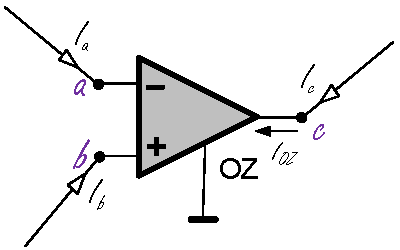
\includegraphics[width=0.6\linewidth]{MMUN_ideal_VFA.pdf}
            \caption[Ideální operační zesilovač typu VFA]{Ideální operační zesilovač typu VFA}
            \label{TEO:fig_MMUN_ideal_VFA}
          \end{figure}
          Ve spodním přídavném řádku je zapsána rovnice
          \begin{equation}\label{TEO:eq_MMUN_VFA}
              0 = 1\cdot U_a - 1\cdot U_b
          \end{equation}
          Výsledek řešení se nezmění, jestliže obě strany této rovnice vynásobíme libovolným 
          nenulovým číslem. Ve spodním řádku tedy může být namísto $[1,-1]$ například $[15,-15]$.
          \begin{figure}[ht!]
            \centering
            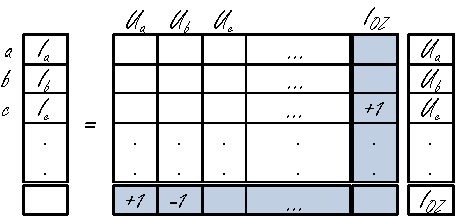
\includegraphics[width=\linewidth]{MMUN_ideal_VFA_matice.pdf}
            \caption[MMUN - pro ideální OPAMP]{MMUN - pro ideální OPAMP typu VFA}
            \label{TEO:fig_MMUN_VFA_matice}
          \end{figure}
          Je-li jeden ze vstupů OZ spojený s referenčním uzlem, neobjeví se příslušné uzlové napětí 
          v rovnicích a proto v posledním řádku bude figurovat jen jedna jednička místo uvedené 
          dvojice. 
          
          Jednička v řádku \emph{c} a sloupci $I_{OZ}$ reprezentuje připočtení proudu $I_{OZ}$ do 
          celkové bilance proudů, vytékající z uzlu \emph{c}.
        
          % --------example: Invertující zesilovač ---------------
          % \label{TEO:ex_InvOpamp01}
            % !TeX spellcheck = cs_CZ
\begin{example}\label{TEO:ex_InvOpamp01}
  Uvažujme invertující zesilovač s ideální operačním zesilovačem typu VFA s naznačenými uzly 
  tak, jak je na obr. \ref{TEO:fig_MMUN_inv_opamp}. Napište rovnice MMUN.
  
   {\centering
    \captionsetup{type=figure}
    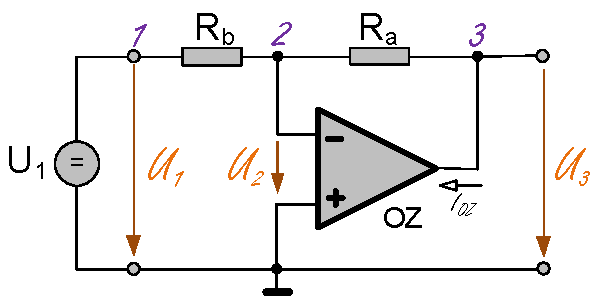
\includegraphics[width=0.7\linewidth]{MMUN_inv_OPAMP.pdf}
    \captionof{figure}{Invertující zesilovač}
    \label{TEO:fig_MMUN_inv_opamp}
    \par}
  
  Rovnice MMUN budou v maticovém zápisu vypadat takto:

    % using \usepackage{array} and command \newcolumntype{C}[1]{>{\centering}m{#1}}!
   {\centering
    \begin{tabular}{|C{0.6cm}|C{1.2cm}|C{0.6cm}|C{0.45cm}|C{0.45cm}|C{.3cm}|c|C{.33cm}|c|}
        \multicolumn{1}{c}{$U_1$}    & \multicolumn{1}{c}{$U_2$}    & \multicolumn{1}{c}{$U_3$}  & 
        \multicolumn{1}{c}{$I_1$}    & \multicolumn{1}{c}{$I_{OZ}$} & \multicolumn{1}{c}{ }      &  
        \multicolumn{1}{c}{x}        & \multicolumn{1}{c}{ }        & \multicolumn{1}{c}{b}       \\
      \cline{1-5}\cline{7-7} \cline{9-9}
      $G_b$  & $-G_b$    &  & -1  &  & \multirow{5}{*}{$\ast$} & $U_1$ & \multirow{5}{*}{=}     & \\
      \cline{1-5} \cline{7-7} \cline{9-9}
      $-G_b$ & $G_a+G_b$ & $-G_a$ &  &   & & $U_2$      &      &                                  \\
      \cline{1-5} \cline{7-7} \cline{9-9}
             & $-G_a$    & $G_a$  &  & 1 & & $U_3$      &      &                                  \\
      \cline{1-5} \cline{7-7} \cline{9-9}
         1   &           &        &  &   & & $I_1$      &      &    $U_{IN}$                      \\
      \cline{1-5} \cline{7-7} \cline{9-9}
             &     1     &        &  &   & & $I_{OZ}$   &      &                                  \\
      \cline{1-5} \cline{7-7} \cline{9-9}
    \end{tabular}
    \par}
  \vspace{1em}
  Předposlední rovnice říká, že uzlové napětí $U_1$ je rovno napětí signálového zdroje $U_{IN}$. 
  Jednička v posledním řádku reprezentuje jednoduchou rovnici $U_2 = 0$. Ačkoliv je obvod poměrně 
  jednoduchý, je pro ruční řešení neefektivní, neboť jsme získali soustavu o 5 rovnic a 5 neznámých.
\end{example}  
          %-------------------------------------------------------

          % --------example: Neinvertující zesilovač -------------
          % \label{TEO:ex_NeinvOpamp01}
            % !TeX spellcheck = cs_CZ
\begin{example}\label{TEO:ex_NeinvOpamp01} 
  Uvažujme neinvertující zesilovač s ideální operačním zesilovačem typu VFA s naznačenými uzly tak, 
  jak je na obr. \ref{TEO:fig_MMUN_neinv_opamp}. Napište rovnice MMUN.

   {\centering
    \captionsetup{type=figure}
    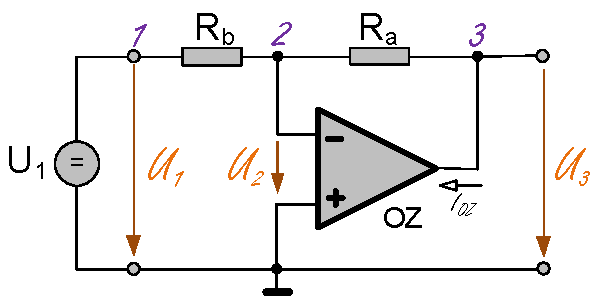
\includegraphics[width=0.7\linewidth]{MMUN_inv_OPAMP.pdf}
    \captionof{figure}{Neinvertující zesilovač}
    \label{TEO:fig_MMUN_neinv_opamp}
    \par}
   % using \usepackage{array} and command \newcolumntype{C}[1]{>{\centering}m{#1}}!
  {\centering
   \begin{tabular}{|C{0.45cm}|C{1.2cm}|C{0.6cm}|C{0.45cm}|C{0.45cm}|C{0.2cm}|c|C{.3cm}|c|}
      \multicolumn{1}{c}{$U_1$} & \multicolumn{1}{c}{$U_2$}   & \multicolumn{1}{c}{$U_3$} & 
      \multicolumn{1}{c}{$I_1$} & \multicolumn{1}{c}{$I_{OZ}$}& \multicolumn{1}{c}{ }     & 
      \multicolumn{1}{c}{x}     & \multicolumn{1}{c}{ }       & \multicolumn{1}{c}{b}     \\ 
      \cline{1-5} \cline{7-7} \cline{9-9}
           &   &   &  -1  &  & \multirow{5}{*}{$\ast$} & $U_1$ & \multirow{5}{*}{=}  &   \\
      \cline{1-5} \cline{7-7} \cline{9-9}
           & $G_a+G_b$ & $-G_a$ &      &   & & $U_2$     &   &                           \\
      \cline{1-5} \cline{7-7} \cline{9-9}
           & $-G_a$    & $G_a$ &       & 1 & & $U_3$     &   &                           \\
      \cline{1-5} \cline{7-7} \cline{9-9}
         1 &           &       &       &   & & $I_1$     &   & $U_{IN}$                  \\
      \cline{1-5} \cline{7-7} \cline{9-9}
           &     1     &       &       &   & & $I_{OZ}$  &   & $U_{IN}$                  \\
      \cline{1-5} \cline{7-7} \cline{9-9}
   \end{tabular}
   \par}
   \vspace{1em}
\end{example}  
          %-------------------------------------------------------
          \newpage
          % --------example: Diferenciální zesilovač -------------
          % \label{TEO:ex_DifOpamp01}
            % !TeX spellcheck = cs_CZ
\begin{mdframed}[style=mdexam]
\begin{example}\label{TEO:ex_DifOpamp01} 
  Uvažujme diferenciální zesilovač s ideální operačním zesilovačem typu VFA s naznačenými 
  uzly tak, jak je na obr. \ref{TEO:fig_MMUN_diff_opamp}. Napište rovnice MMUN.

   {\centering
    \captionsetup{type=figure}
    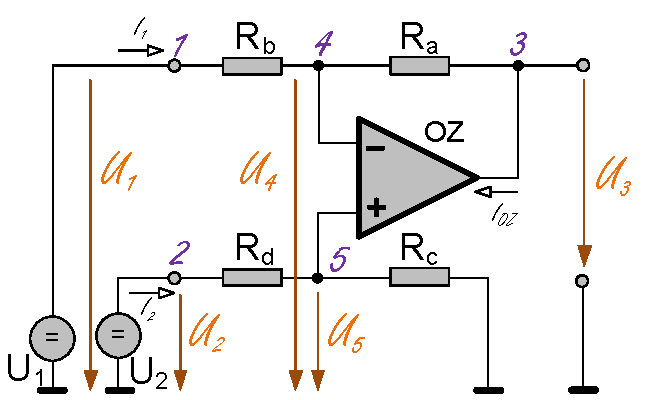
\includegraphics[width=0.7\linewidth]{MMUN_diff_OPAMP.pdf}
    \captionof{figure}{ Diferenciální zesilovač}
    \label{TEO:fig_MMUN_diff_opamp}
    \par}

    % using \usepackage{array} and command \newcolumntype{C}[1]{>{\centering}m{#1}}!
    {\centering
    \begin{tabular}{|C{0.6cm}|C{0.6cm}|C{0.6cm}|C{1.2cm}|C{0.6cm}|C{0.45cm}|C{0.45cm}|C{0.45cm}|}
        \multicolumn{1}{c}{$U_1$}  & \multicolumn{1}{c}{$U_2$}   & \multicolumn{1}{c}{$U_3$}  & 
        \multicolumn{1}{c}{$U_4$}  & \multicolumn{1}{c}{$U_5$}   & \multicolumn{1}{c}{$I_1$}  & 
        \multicolumn{1}{c}{$I_2$}  & \multicolumn{1}{c}{$I_{OZ}$}                      \\
        \hline
        $G_b$  &        &        & $-G_b$    &         & \(-1\) &        &             \\
        \hline
               & $G_d$  &        &           & $-G_d$  &        & \(-1\) &             \\
        \hline
               &        &  $G_a$ & $-G_a$    &         &        &        &             \\
        \hline 
        $-G_b$ &        & $-G_a$ & $G_a+G_b$ &         &        &        &             \\
        \hline
               & $-G_d$ &        & $G_c+G_d$ &         &        &        &             \\
        \hline
               &        &        &  \(-1\)   &  \(1\)  &        &        &             \\
        \hline
         1     &        &        &           &         &        &        &             \\
        \hline   
               & \(1\)  &        &           &         &        &        &             \\
        \hline    
    \end{tabular}
    \par}
\end{example}
\end{mdframed}  
          %-------------------------------------------------------

  \section{Analýza pomocí numerického simulátoru}
    \subsection{Analýza „DC“ neboli stejnosměrná analýza}
    \subsection{Rozšiřující typy analýz}
      \subsubsection{Citlivostní analýza („Sensitivity“)}
        Je počítána \emph{stejnosměrná citlivost} jedné nebo více veličin, vyjádřené vzorcem nebo 
        vzorci, na jednu nebo více vstupních proměnných.

          % --example: Citlivostní analýza napěťový děliče -------
          % \label{TEO:ex_CitDiveder01}
            % !TeX spellcheck = cs_CZ
\begin{example}\label{TEO:ex_CitDiveder01}
  V elektronických soustavách se největších přesností dosahuje u rezistorů, kde je standardně 
  zaručována chyba menší než 1\%, u přesných 0.1\% a u velmi přesných 0.01\%.

   {\centering
    \captionsetup{type=figure}
    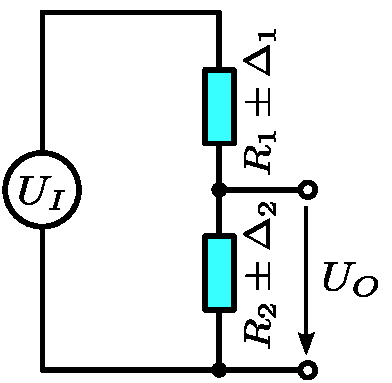
\includegraphics[width=0.4\linewidth]{voltage_divider.pdf}
    \captionof{figure}{ }
    \label{TEO:fig_voltage_divider}
    \par}

  Bude nás zajímat jaký vliv má tolerance rezistorů na výsledný poměr výstupního ku vstupnímu 
  napětí a také, zda-li při různě zvoleném poměru těchto rezistorů se bude měnit velikost chyby, 
  ačkoliv budou mít stejnou přesnost. Intuitivně předpokládáme, že  nejnepříznivější situace  
  nastane, když hodnoty použitých rezistorů padnou na opačné strany tolerančních pásem, jenž 
  reprezentuje $\Delta_1$ a $\Delta_2$ tj. $R_2 - \Delta_2R_2$ a $R_1 + \Delta_1R_1$ nebo $R_2 + 
  \Delta_2R_2$ a $R_1 - \Delta_1R_1$. V obou případech bude chyba stejná, proto si vybereme 
  například první případ a zapíšeme (rov. \ref{TEO:eq_divider_1}).
  \begin{equation}\label{TEO:eq_divider_1}
    \frac{U_o}{U_i} = \frac{R_2-\Delta_2 R_2}{R_1+\Delta_1 R_1+R_2-\Delta_2 R_2}
  \end{equation}
  a po úpravě
  \begin{equation*}
     \frac{U_o}{U_i} = \frac{(1-\Delta_2) R_2}{(1+\Delta_1) R_1+(1-\Delta_2) R_2}
  \end{equation*}
  Polynom ve jmenovateli rozvineme do následující podoby
  \begin{align*}
     [(1+\Delta_1) &+ (1-\Delta_2)](R_1+R_2)                \\
                   &= (1+\Delta_1)R_1 + (1-\Delta_2)R_2     \\
                   &+ (1+\Delta_1)R_2 + (1-\Delta_2)R_1     \\
   (1+\Delta_1)R_1 &+ (1-\Delta_2)R_2                       \\
                   &= [(1+\Delta_1)+(1-\Delta_2)](R_1+R_2)  \\
                   &- (1+\Delta_1)R_2 - (1-\Delta_2)R_1 
  \end{align*}
  a získáme %Further simplification of the denominator yields
  {\footnotesize
  \begin{equation*}
      \dfrac{U_o}{U_i}\ =
        \dfrac{(1-\Delta_2) R_2}{[(1+\Delta_1) + (1-\Delta_2)](R_1+R_2) - 
        [(1+\Delta_1) R_2\ +\ (1-\Delta_2) R_1] }
  \end{equation*}
  } %
  Nyní vydělíme jmenovatel i čitatel $(R_1 + R_2)$ a dostaneme 
  % Next divide both numerator and denominator by R1 + R2
  \begin{equation*}\label{TEO:eq_divider_2}
    \frac{U_o}{U_i}\ =\dfrac{\dfrac{(1-\Delta_2) R_2}{R_1+R2}}{[(1+\Delta_1)+(1-\Delta_2)] - 
    \dfrac{[(1+\Delta_1) R_2\ +\ (1-\Delta_2) R_1]}{R_1+R_2} }
  \end{equation*}
  Standardně rezistory volíme se stejnou tolerancí, tedy $\Delta_1 = \Delta_2 = \Delta$ a získáme 
  výslednou rovnici pro poměr $\frac{U_o}{U_i}$ 
  % Based on the assumption that both $\Delta1 = \Delta2 = \Delta$ then it should be possible to  
  % further simplify the expression for Vo/Vi:
  \begin{equation}
     \dfrac{U_o}{U_i} = \dfrac{\dfrac{(1-\Delta) R_2}{R_1+R_2}}{[(1+\Delta)+(1-\Delta)] - 
     \dfrac{[(1+\Delta)R_2 + (1-\Delta) R_1]}{R_1+R_2} }
  \end{equation}

  Řekněme například, že pro návrh děliče máme k dispozici rezistory s tolerancí 1\% a vstupní 
  napětí je 1 V. Obvod, ve kterém je dělič použit, umožňuje volit různé poměry, ale jejich součet 
  je konstantní. Na otázku jaký poměr zvolit, abychom při dané toleranci rezistorů dostali 
  výstupní napětí s největší přesností odpovídá následující tabulka.
  \vspace{1em}
  
  {\centering
   \setlength{\tabcolsep}{5pt}
   \begin{tabular}{|c|c|c|c|}
      \hline
        $R_1$                 & $1 k\Omega$  & $10 k\Omega$     & $19 k\Omega$   \\
      \hline
        $R_2$                 & $19 k\Omega$ & $10 k\Omega$     & $1 k\Omega$    \\
      \hline
        $U_{out}$             & 0,950        & 0,500            & 0,050          \\
      \hline
        $U_{out}^*$           & 0,949        & 0,495            & 0,049          \\
      \hline
        $\varepsilon_r [\%]$  & 0,101        & 1,000            & 1,883          \\
      \hline
   \end{tabular}
  \par}
  \vspace{1em}

  % Let's compare this answer to the formula I gave in a previous post using differentials. The  
  % relevant differential is
  % \begin{equation}\label{TEO:eq_divider_8}
  %   dV_0 = ( \frac{V}{R_1+R_2} - \alpha ) dR_1 - \alpha dR_2 + \frac{R_1}{R_1+R_2} dV
  % \end{equation}
  % where
  % \begin{equation}\label{TEO:eq_divider_9}
  %   \alpha = \frac{R_1 V}{(R_1+R_2)^2}
  % \end{equation}
\end{example}  
    
          %-------------------------------------------------------
%} % \tikzset

%---------------------------------------------------------------------------------------------------
\printbibliography[title={Seznam literatury}, heading=subbibliography]
\addcontentsline{toc}{section}{Seznam literatury}
%========== Kapitola: Přechodné děje ==============================================================
  % !TeX spellcheck = cs_CZ
% file: prechod_deje.tex
%{\tikzset{external/prefix={tikz/TEO/}}
% \tikzset{external/figure name/.add={ch10_}{}}
%========= Kapitola: Dynamické pochody v lineárních obvodechů ======================================
\setchaptertoc
\chapter{Dynamické pochody v lineárních obvodech}

  \section{Fyzikální podstata přechodných dějů}
    V obvodu, který je v ustáleném stavu, nechť dojde buďto
    \begin{itemize}
      \item ke změně parametru aktivního prvku (např. připojení nebo odpojení zdroje napětí nebo  
            proudu),
      \item ke změně parametru pasivního prvku (např. zvětšení nebo zmenšení odporu, indukčnosti  
            nebo kapacity),
      \item ke změně topologické struktury (např. přerušení větve, spojení větve nakrátko, připojení 
            další větve).
    \end{itemize}
    Kteroukoliv z uvedených změn dostaneme nový obvod jemuž přísluší nový \emph{ustálený stav}; 
    tento stav však nenastane okamžitě. Zmíněná změna přivede obvod do \emph{ne\-us\-tá\-le\-né\-ho 
    stavu}, v němž odezvy napětí a proudů - nazýváme je \textbf{přechodnými jevy} - se postupně 
    přibližují k hodnotám nového ustáleného stavu. Přechodné jevy, ač - přesně vzato - probíhají v 
    nekonečně dlouhé době, jsou v praxi jevy krátkodobými, neboť odezvy se trvale "dostatečně 
    těsně" přiblíží k hodnotám nového stavu již v poměrně krátké době - v běžných případech jsou to 
    mikrosekundy až milisekundy.

    Naskýtá se otázka, proč odezvy obvodu obecně nepřecházejí z původního do nového ustáleného 
    stavu skokem a proč dochází k neustálenému stavu obvodu. Obvod má elektromagnetickou energii 
    $W(t)$, která je součtem energií elektrického pole kondenzátoru $W_e(t)$ a energií magnetického 
    pole cívek $W_m(t)$. Elektromagnetická energie obvodu
    \begin{equation*}
      W(t)=\sum_kW_{e_k}(t)+\sum_kW_{m_k}(t)
    \end{equation*}
    je tedy funkcí napětí na jeho kondenzátorech a proudů v jeho cívkách. Protože tyto veličiny 
    určují energetický stav obvodu, nazýváme je \textbf{stavovými veličinami}.

    \begin{figure}[ht!]
       \centering
       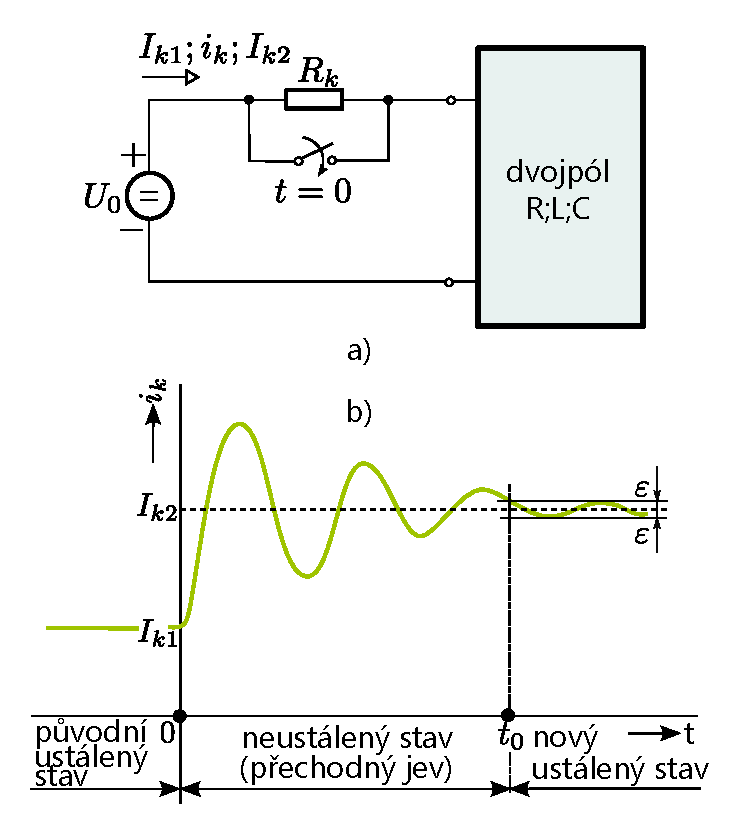
\includegraphics[width=0.8\linewidth]{prechodny_dej.pdf}
       \caption[Přechodný jev]{K objasnění pojmů "neustálený stav" a "přechodný jev"}
       \label{TEO:fig_prechodny_dej}
    \end{figure}

    Elektrické výkony $P$ v reálném elektrickém obvodu mají z fyzikálních důvodů vždy konečnou 
    hodnotu. U obvodů, které jsou dostatečně adekvátními modely respektujícími tuto skutečnost 
    (nazýváme je obvody s konečnými výkony) je to postačující podmínkou pro to, aby jejich energie 
    $W = W(t)$ byla spojitou funkcí času (neboť $P = \frac{dW}{dt}$). Z uvedených vztahů pro 
    energii obvodu $W(t)$ je patrné, že $W = W(t)$ bude spojitou funkcí, jsou-li stavové veličiny 
    \emph{spojitými funkcemi}. To znamená, že hodnota stavových veličin v okamžiku před vznikem 
    přechodného jevu je táž jako v okamžiku po jeho vzniku. Pro přechodný jev v okamžiku $t=0$ 
    platí tedy
    \begin{equation}\label{TEO:eq_spojite_fce}
      \lim_{t\rightarrow0_-}u_c(t)= \lim_{t\rightarrow0_+}u_c(t); \quad  
      \lim_{t\rightarrow0_-}i_L(t)= \lim_{t\rightarrow0_+}i_L(t)
    \end{equation}

     \subsection{Přechodné jevy v jednodušších obvodech; charakteristické pojmy a vlastnosti}
        % --------example: Transformátor -----------------------
        % \label{TEO:exam005}
          % !TeX spellcheck = cs_CZ
\begin{example}\label{TEO:exam005} \textbf{Transformátor}: \newline
  Na primární vinutí vzduchového transformátoru s činitelem $k < 1$ je v čase $t=0$ připojen zdroj 
  napětí $U_1 = konst$. Formulujte postup pro výpočet odezev $i_1(t)$ a $i_2(t)$ pro obecné 
  parametry zapojení a výsledky ověřte simulací pro následující hodnoty: $U_1 = 1V, R_1 = 1\Omega, 
  R_2 = 4\Omega, $ transformátor má převod $1:3$.
  
  {\centering
   \captionsetup{type=figure}
   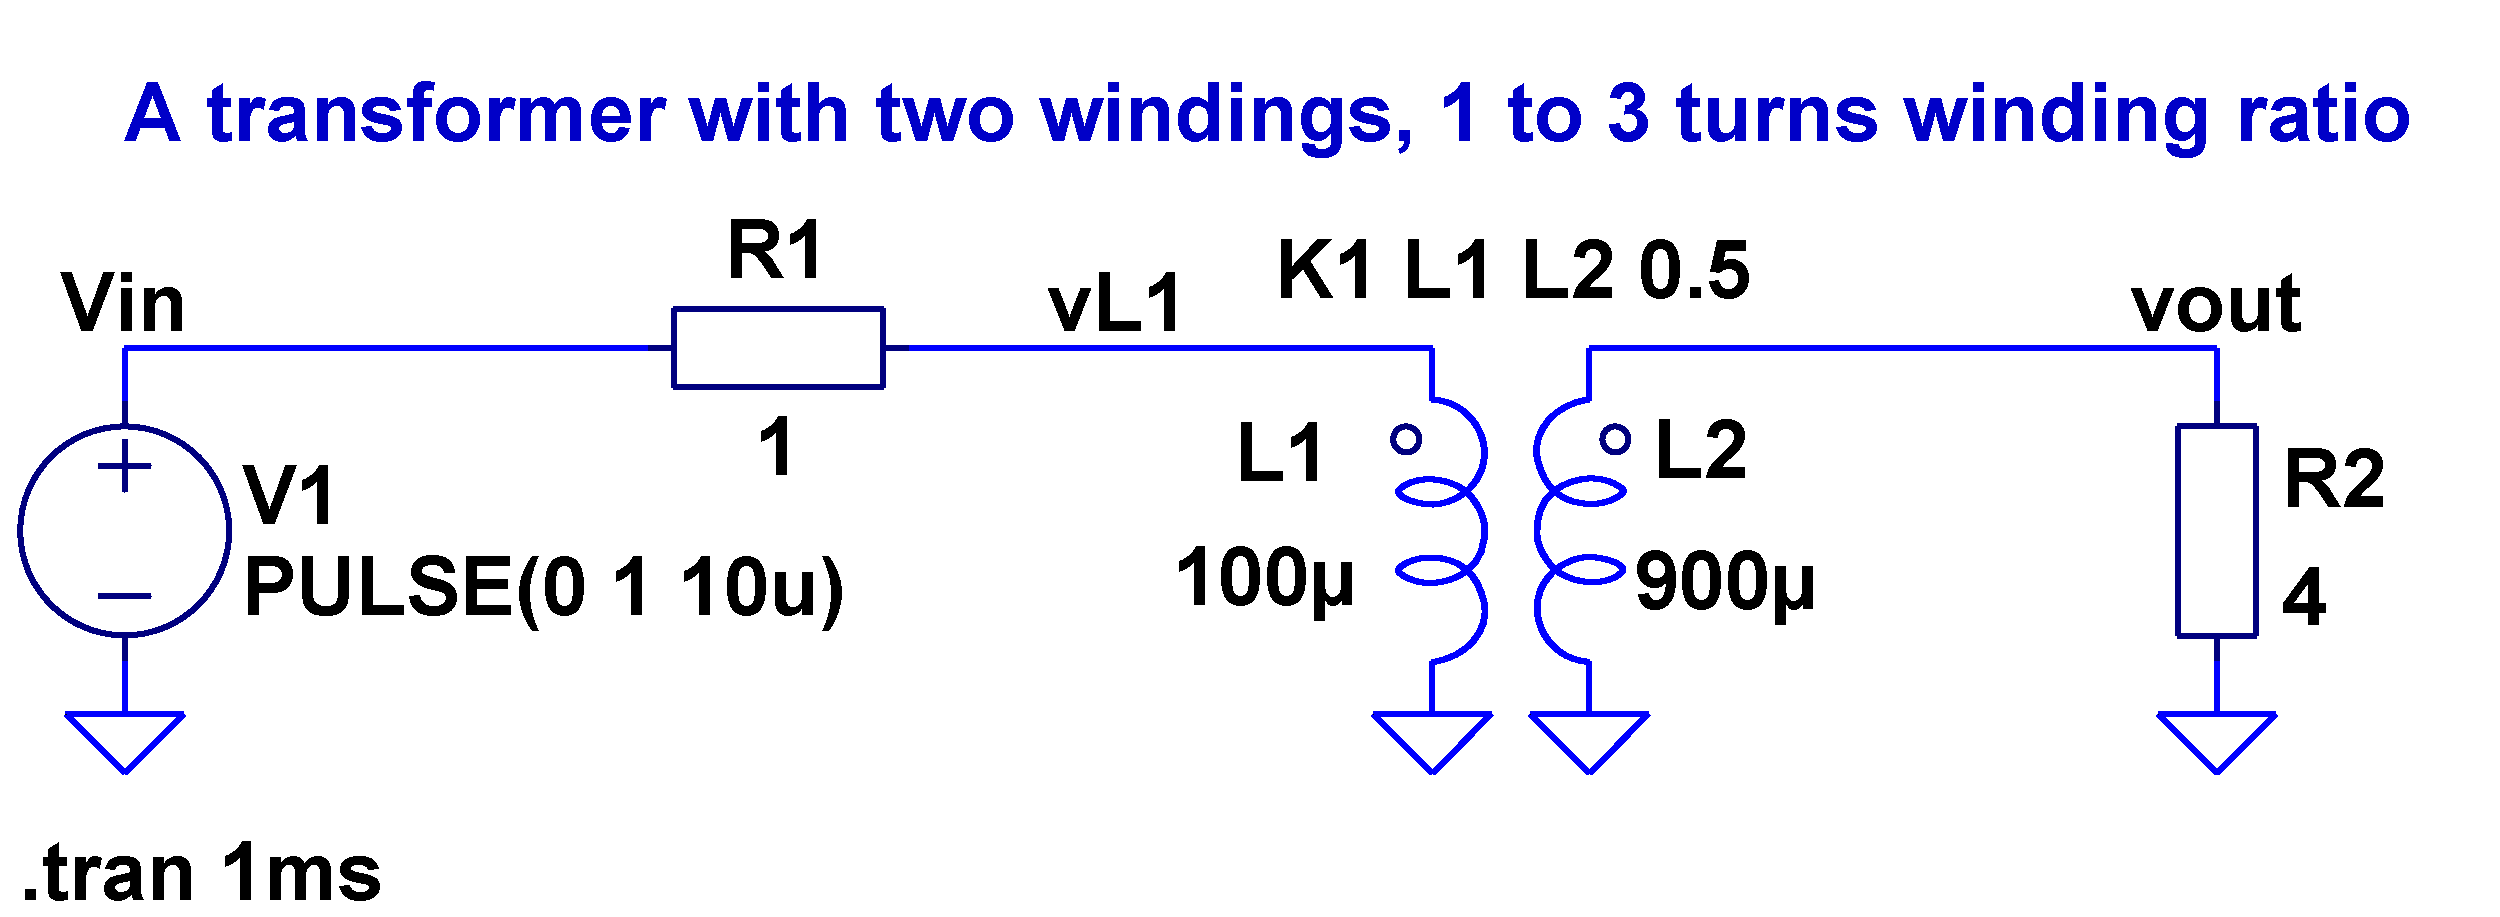
\includegraphics[width=0.9\linewidth]{Ideal_Trf_step_response_LTspice.pdf}
   \captionof{figure}{\texttt{Transformer.asc}: Zapojení vzduchového transformátoru
              pro simulaci v programu LTSpice}
   \label{TEO:fig_trafo_int_uprim}
   \par}
  
  \textbf{Klasické řešení}: Podle II. Kirchhoffova zákona platí soustava rovnic:
  \begin{subequations}\label{TEO:eq_trafo_IIKz}
    \begin{align}
      R_1i_1 + L_1\frac{di_1}{dt} + L_{12}\frac{di_2}{dt} &= U_1 \\
      R_2i_2 + L_2\frac{di_2}{dt} + L_{12}\frac{di_1}{dt} &= 0
    \end{align}
  \end{subequations}
  
  \begin{equation}\label{TEO:eq_char_rce}
  \left(
  \begin{array}{cc}
  R_1 + L_1\lambda & L_{12}\lambda  \\
  L_{12}\lambda    & R_2 + L_2\lambda
  \end{array}
  \right) = 0
  \end{equation}
  \begin{subequations}\label{TEO:eq_char_rce_solve}
    \begin{align}
      (R_1 + L_1\lambda) - L_{12}^2\lambda^2                                      &= 0      \\
      R_1R_2 + (L_1R_2 + L_2R_1)\lambda + L_1L_2\lambda - L_{12}^2\lambda^2       &= 0      \\
      \lambda^2(L_1L_2-L_{12}^2)+(L_1R_2+L_2R_1)\lambda +R_1R_2                   &= L_1L_2 \\
      \lambda^2(\frac{L_1L_2-L_{12}^2}{L_1L_2})+
      (\frac{L_1R_2+L_2R_1}{L_1L_2})\lambda +\frac{R1R2}{L_1L_2}                  &= 0
    \end{align}
  \end{subequations}
  Zavedeme-li $\tau_1 = \frac{L_1}{R_1}, \tau_2 = \frac{L_2}{R_2}$,
  $k=\frac{L_12}{\sqrt{L_1L_2}}, k^2=\frac{L_12^2}{L_1L_2}$, $\sigma = 1-k^2$ dostaneme
  \begin{subequations}\label{TEO:eq_trafo_vysl_rce}
    \begin{align}
      \sigma\lambda^2 + \left(\frac{1}{\tau_1}+\frac{1}{\tau_2}\right)\lambda + 
      \frac{1}{\tau_1}\frac{1}{\tau_2} = 0                                                 \\
      \lambda^2 + \frac{1}{\sigma}\left(\frac{1}{\tau_1}+\frac{1}{\tau_2}\right)\lambda + 
      \frac{1}{\sigma\tau_1\tau_2} = 0
    \end{align}
  \end{subequations}
  Je-li $\lambda_1 = -\beta+\alpha$ a $\lambda_2 = -\beta-\alpha$
  \begin{subequations}
    \label{TEO:eq_trafo_alphabeta}
    \begin{align}
    \alpha &= \frac{1}{2\sigma}
    \left(\frac{1}{\tau_1}+ 
    \frac{1}{\tau_2}\right)            \label{TEO:eq_trafo_alphabeta_a}     \\ 
    \beta  &= \frac{1}{2\sigma}
    \sqrt{\left(\frac{1}{\tau_1}+
      \frac{1}{\tau_2}\right)^2+
      \frac{4\sigma}{\tau_1\tau_2}}      \label{TEO:eq_trafo_alphabeta_b}
    \end{align}
  \end{subequations}
  Jelikož $k<1$; je $0<\sigma<1$; rozborem rovnice \ref{TEO:eq_trafo_alphabeta_b} plyne, že pak
  je $\alpha\neq0$, reálné. Soustava rovnic \ref{TEO:eq_trafo_IIKz} má tedy obecné řešení
  \begin{subequations}\label{TEO:eq_trafo_obecne_res}
    \begin{align}
      i_1(t) &= i_{1o} +i_{1p} = K_1e^{\lambda_1t} + K_2e^{\lambda_2t} +\frac{U_0}{R} \\
      i_2(t) &= i_{2o} +i_{2p} = K_3e^{\lambda_1t} + K_4e^{\lambda_2t}
    \end{align}
  \end{subequations}
  Integrační konstanty $K_1, K_2, K_3$ a $K_4$ určíme z matematických počátečních podmínek:
  $i_1(0)=i_2(0)=0$ (což jsou zároveň fyzikální počáteční podmínky) a $\frac{di_1}{dt}|_{t=0}, 
  \frac{di_2}{dt}|_{t=0}$, které určíme z rovnic \ref{TEO:eq_trafo_IIKz} pro $t=0$:
  \begin{subequations}\label{TEO:eq_trafo_didt_t0}
    \begin{align}
      L_1i_1'+L_{12}i_2' &= U_0 \Longrightarrow i_1' = \left(\frac{U_0-L_{12}i_2'}{L_1}\right)\\
      L_2i_2'+L_{12}i_1' &= 0
    \end{align}
  \end{subequations}
  Dále postupujeme tak, že do druhé rovnice dosadíme vyjádřenou první derivaci primárního
  proudu z první rovnice a získáme vztah pro první derivaci sekundárního proudu v čase $t=0$:
    \begin{subequations}\label{TEO:eq_trafo_dev_i1i2}
    \begin{align}
      \frac{di_1}{dt}|_{t=0} &=   \frac{L_{2}}{L_1L_2-L_{12}^2}U_0                        \\
      \frac{di_2}{dt}|_{t=0} &=  -\frac{L_{12}}{L_1L_2-L_{12}^2}U_0
    \end{align}
  \end{subequations}
  Aplikací těchto počátečních podmínek na obecné řešení \ref{TEO:eq_trafo_obecne_res} plynou
  vztahy
  \begin{subequations}
    \begin{align}
    i_1(0)                            &= K_1 + K_2 +\frac{U_0}{R}                         \\
    \frac{L_{2}}{L_1L_2-L_{12}^2}U_0  &= \lambda_1K_1 + \lambda_2K_2                      \\
    i_2(0)                            &= K_3 + K_4                                        \\
   -\frac{L_{12}}{L_1L_2-L_{12}^2}U_0 &= \lambda_1K_3 + \lambda_2K_4
    \end{align}
  \end{subequations}
  Z první a třetí rovnice vypočítáme $K_1; K_2$, ze druhé a čtvrté rovnice $K_3; K_4$.
  Do\-sa\-ze\-ním do rovnice \ref{TEO:eq_trafo_obecne_res} dostaneme po úpravě odezvy $i_1(t)$
  a $i_2(t)$. Speciálně pro $R_1=R_2=R$;$L_1=L_2=L$ je
  \begin{subequations}\label{TEO:eq_trafo_solved_RL}
    \begin{align}
      i_1(t) &= \frac{U_0}{2R}\left(2-e^{-\frac{t}{\tau_3}}-e^{-\frac{t}{\tau_4}}\right) \\
      i_2(t) &= \frac{U_0}{2R}\left(-e^{-\frac{t}{\tau_3}}+e^{-\frac{t}{\tau_4}}\right)
    \end{align}
  \end{subequations}
  kde je $\tau_3 = \frac{L + L_{12}}{R}; \tau_4 = \frac{L - L_{12}}{R}$
  
  \textbf{Operátorové řešení}: Laplaceovou transformací rovnice \ref{TEO:eq_trafo_IIKz}
  dostáváme
  \begin{subequations}\label{TEO:eq_trafo_laplace}
    \begin{align}
      (R_1 + pL_1)I_1(p)+pL_{12}I_2(p)   &= \frac{U_0}{p} \\
      pL_{12}I_1(p) + (R_2 + pL_2)I_2(p) &= 0
    \end{align}
  \end{subequations}
  Zavedeme $\sigma; \tau_1; \tau_2$, vypočítáme obrazy proudů a jejich zpětnou transformací
  do\-sta\-ne\-me rovnice pro odezvy $i_1(t)$ a $i_2(t)$.
  
  {\centering
   \captionsetup{type=figure}
   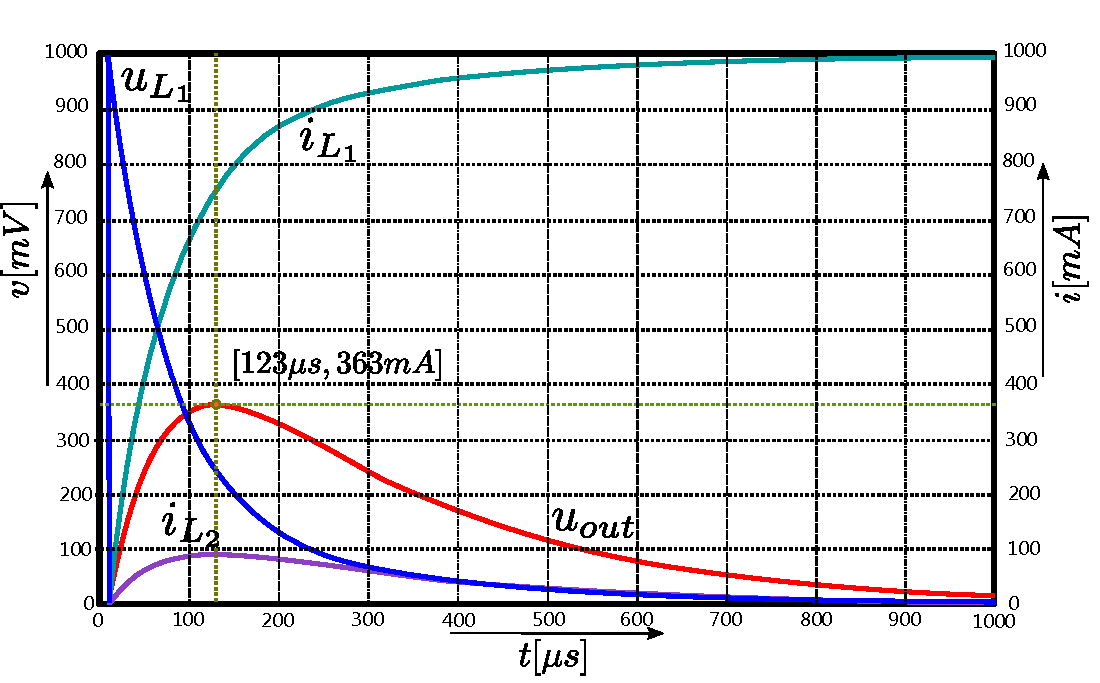
\includegraphics[width=1\linewidth]{Ideal_Trf_step_response_K05.pdf}
   \captionof{figure}{Odezva na jednotkový skok transformátoru s parametry: $k=0.5, L_1 = 100 \mu 
             H, L_2 = 900 \mu H$}
  \label{figure:trafo_int_uprim}
  \par}
\end{example}

  
        %-------------------------------------------------------

        % --------example: Obvod s kondenzátorem ---------------
        % \label{TEO:ex_10_8}
        % % !TeX spellcheck = cs_CZ
\begin{example}\label{TEO:ex_10_8} Najděte odezvu napětí na kondenzátoru $u_c(t)$ obvodu na
  obrázku \ref{TEO:fig_cir_10_8} pro $t>0$. (zdroj \cite[s.~456]{Dorf}) 
  
  {\centering
   \captionsetup{type=figure}
   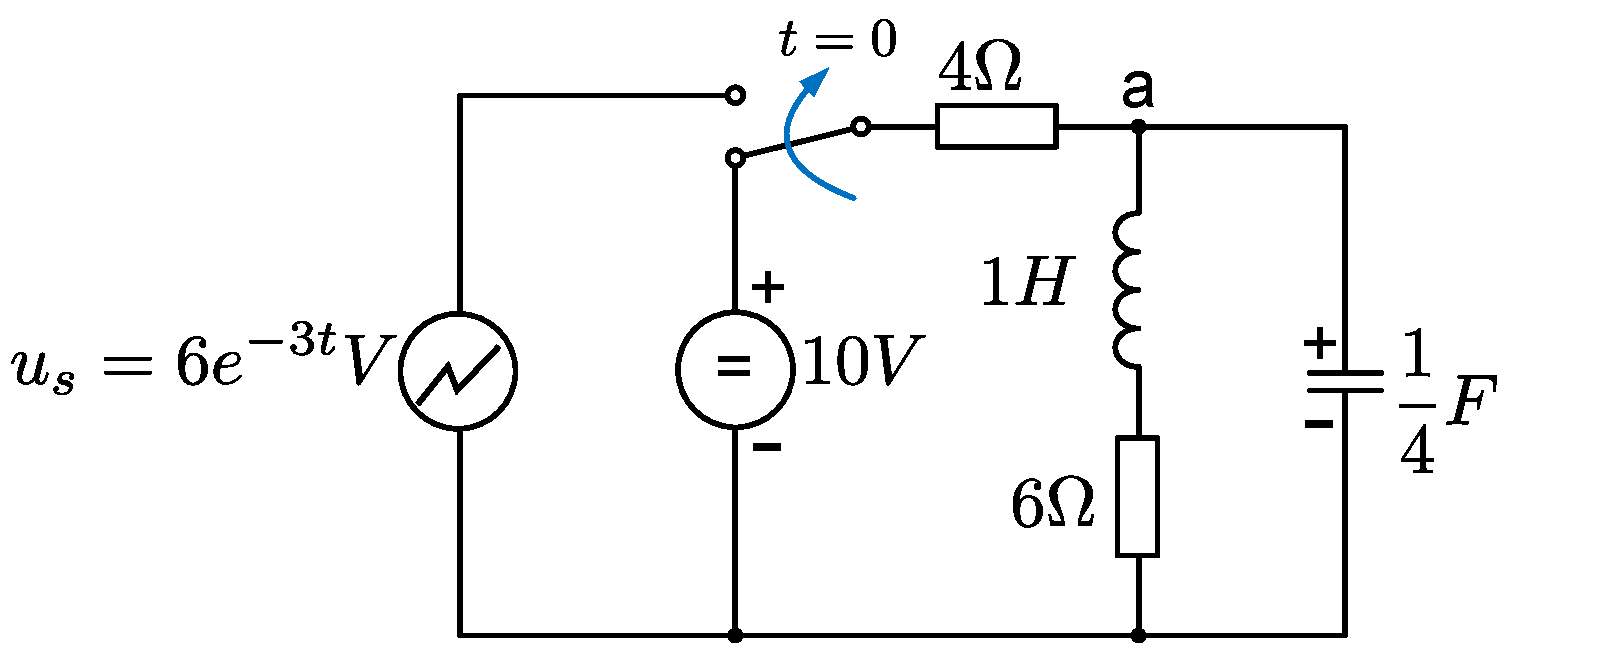
\includegraphics[width=1\linewidth]{response_ex10_8_RLC_cir.pdf}
   \captionof{figure}{Obvod k příkladu \ref{TEO:ex_10_8}}
   \label{TEO:fig_cir_10_8}
   \par}
  
  \textbf{Řešení:} Nejdříve stanovíme počáteční podmínky, které vyplývají z ustáleného stavu
  v době $t = 0^-$. Obvod na obr. \ref{TEO:fig_cir_10_8} můžeme překreslit do podoby na obr.
  \ref{TEO:fig_cir_10_8_steady} 
  
  {\centering
   \captionsetup{type=figure}
   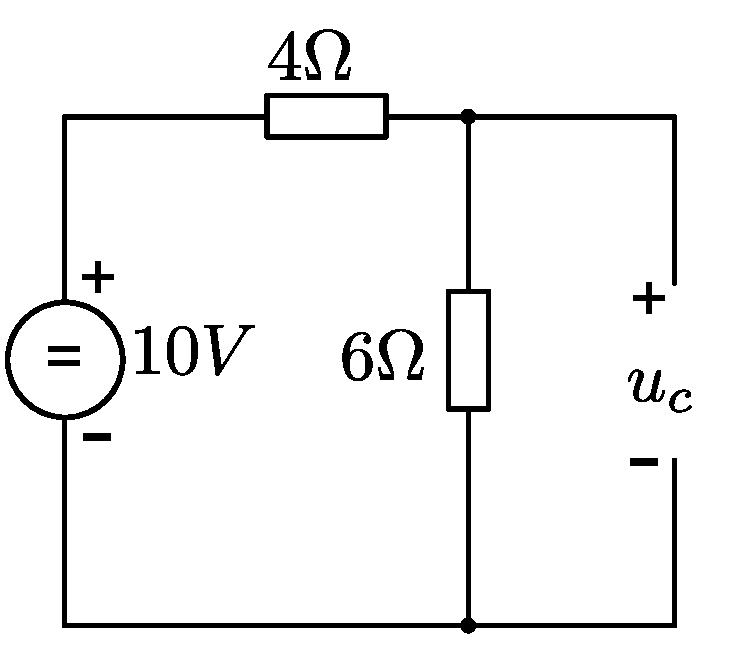
\includegraphics[width=0.4\linewidth]{response_ex10_8_steady.pdf}
   \captionof{figure}{Obvod k příkladu \ref{TEO:ex_10_8}}
   \label{TEO:fig_cir_10_8_steady}
   \par}
  \begin{equation}\label{TEO:eq_10_8_vysledek}
  u_c(t) = \frac{44}{3}e^{-2t}+\frac{1}{3}e^{-5t} - 9e^{-3t} \qquad [V]
  \end{equation}
\end{example}  
        %-------------------------------------------------------
            
  %--------------------- Přechodný jev kmitavého obvodu --------------------------------------------
  \section{Přechodný jev kmitavého obvodu}
    Kmitavým obvodem máme na mysli obvod s jedním stupněm volnosti, složeného z odporu $R$,
    kapacity $C$ a indukčnosti $L$, zapojených v sérii. Je jedním z nejdůležitějších případů
    elektrotechnické praxe. Dosud probírané případy (obvod \emph{RL} a \emph{RC}) jsou vždy určitým
    zjednodušením úplného obvodu s jedním stupněm volnosti, vzniklé tak, že buď indukčnost obvodu,
    nebo kapacita jsou zanedbatelné vzhledem k ostatním prvkům. Rozbor přechodného stavu kmitavého
    obvodu (dále stručně obvodu \emph{RLC}) umožňuje stanovit směrnice pro možnost tohoto
    zjednodušení a jeho důsledky.
    
    \luagraphic[0.5]{teo_fig027.pdf}{Schéma sériového kmitavého obvodu}{teo:fig027}

    Zopakujme, že přechodný stav, je vždy dán superpozicí nového ustáleného stavu a vlastní
    přechodné složky, jejíž průběh závisí jen na vlastnostech obvodu a počátečních podmínkách (a
    nikoliv na průběhu vstupního signálu), proto nejdříve budeme řešit tzv. \emph{volný stav
    obvodu}, tj. stav, kdy vnější působení na vstupu je nulové. Za těchto okolností může v obvodu
    existovat přechodný jev, je-li v obvodu (tj. v akumulačních prvcích) na počátku nahromaděná
    určitá energie. Vzhledem k tomu, že to může být jednak energie elektrického pole v kondenzátoru,
    jednak energie magnetického pole v cívce, je počáteční stav úplně určen, známe-li hodnoty napětí
    na kapacitě a proudu v indukčnosti v počátečním okamžiku; matematicky vyjádřeno, stanovíme
    počáteční podmínky vždy ve tvaru
    \begin{equation}\label{TEO:eq_RLC_00}
      u_C(0) = U_{C_0} \qquad i(0) = I_0.
    \end{equation}    
    Protože za volného stavu jsou vstupní svorky spojeny \emph{nakrátko}, je rovnice pro proud v
    obvodu
    \begin{align}\label{TEO:eq_RLC_01}
       u_R + u_L + u_C                                    &= 0 \\
       Ri + L\der{i}{t} +\frac{1}{C}\int_0^tidt + U_{C_0} &= 0
    \end{align}     
    Řešení provedeme pomocí Laplaceovy transformace. K přihlédnutím  k počátečním podmínkám
    \ref{TEO:eq_RLC_01} dostaneme rovnici
    \begin{equation}\label{TEO:eq_RLC_02}
      I(p)(R + Lp + \frac{1}{pC}) = I_0L - \frac{U_{C_0}}{p},
    \end{equation}     
    a z ní 
    \begin{equation}\label{TEO:eq_RLC_03}
      I(p) = \frac{pCLI_0 - CU_{C_0}}{p^2LC + pRC + 1}.
    \end{equation}

%} % tikzset
%---------------------------------------------------------------------------------------------------
%========== Kapitola: Obvody v harmonickém ustáleném stavu ========================================
  % !TeX spellcheck = cs_CZ
%=====================Kapitola: Obvody v harmonickém ustáleném stavu=======================
\chapter{Obvody v harmonickém ustáleném stavu}
  V této kapitole se seznámíme se \emph{symbolicko-komplexní metodou} (\texttt{SKM}), jež má
  základní důležitost pro teorii obvodů v harmonickém ustáleném stavu. Potom prozkoumáme vlastnosti
  jednodušších obvodů v tomto stavu a metody jejich analýzy. Posléze pojednáme o elektrickém výkon
  v obvodech a o nejdůležitějších otázkách přenosu energie \cite[s.~60]{Mayer1978}.
  
  \section{Periodické veličiny a jejich charakteristické hodnoty}
    \emph{Periodickou veličinou} nazýváme takovou veličinu $v$, jejíž závislost na čase lze
    vyjádřit periodickou funkcí, pro níž existuje konstanta $T>0$ taková, že pro každé $t$ platí
    vztah
    \begin{equation}\label{TEO:eq_harm01}
      v(t+T) = v(t),    
    \end{equation}  
    Konstanta $T$ se nazývá \textbf{perioda} resp. \emph{doba kmitu}. V aplikacích se zpravidla
    používá nejmenší kladná perioda, tzv. \emph{základní perioda}; pro stručnost budeme hovořit
    pouze o periodě. Je-li dána periodická veličina na jakémkoliv intervalu $(t_0, t_0+T)$, je tím
    zřejmě definována pro všechna $t>t_0$. Průběh veličiny $v$ na jakémkoliv intervalu délky $T$ se
    nazývá \emph{cyklem}. Počet cyklů za jednotku času (za sekundu) udává \textbf{kmitočet}, nebo
    též \emph{frekvenci} periodické veličiny
    \begin{equation}\label{TEO:eq_harm02}
      f = \frac{1}{T},
    \end{equation}
    V elektrotechnice rozdělujeme periodické veličiny do dvou skupin:
    \begin{figure}[ht!] % \ref{teo:fig029}
       \centering
       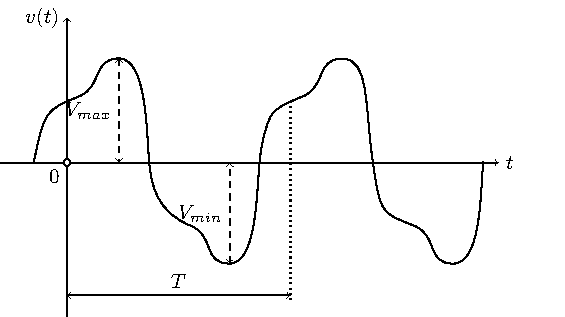
\includegraphics[width=0.8\linewidth]{teo_fig029.pdf}
       \caption{Příklad periodické veličiny $v=v(t)$ pro kterou platí $v(t+T)=v(t)$}
       \label{teo:fig029}
    \end{figure}

    \begin{figure}[ht!] % \ref{teo:fig030}
       \centering
       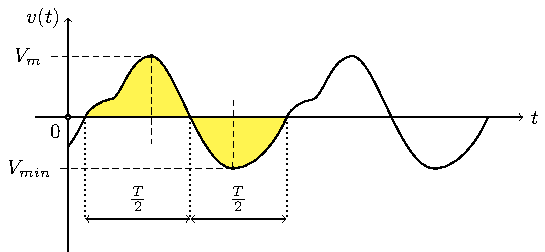
\includegraphics[width=0.8\linewidth]{teo_fig030.pdf}
       \caption{Časový průběh \textbf{střídavé veličiny} $v=v(t)$, pro kterou platí, že obsahy ploch
                v jednom cyklu nad osou $t$ a pod osou $t$ jsou totožné}
       \label{teo:fig030}
    \end{figure}

    \begin{itemize}
      \item Veličiny $v$, jež během svého cyklu \emph{změní znaménko} (obr.\ref{teo:fig029})
            nazýváme \textbf{kmitavé}. \emph{Speciálním případem} kmitavých veličin jsou
            \textbf{střídavé veličiny}, jež mají tu vlastnost, že po dobu $T/2$ jsou trvale kladné,
            po dobu $T/2$ naopak záporné a obsahy ploch omezených grafem funkce $v=v(t)$ v jednom
            cyklu nad osou $t$ a pod osou $t$ jsou \emph{totožné} (obr. \ref{teo:fig030}).
      \item Veličiny $v$, jež \emph{nemění své znaménko}, tj. jsou trvale kladné nebo trvale
            záporné (obr.\ref{teo:fig031}) nazýváme \textbf{pulzující}. \emph{Speciálním případem}
            jsou \textbf{stejnosměrné veličiny}, které nemění svou hodnotu, tj. $v=konst$
            (obr.\ref{teo:fig031} (b)).
    \end{itemize} 

    \begin{figure}[ht!] % \ref{teo:fig031}
       \centering
       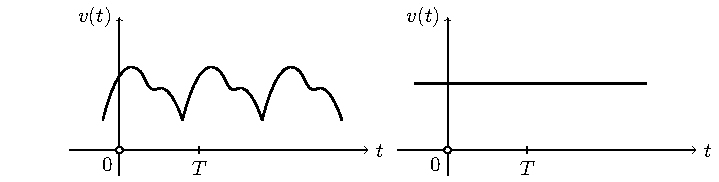
\includegraphics[width=0.8\linewidth]{teo_fig031.pdf}
       \caption{Časový průběh pulsující periodické veličiny a konstantní veličiny}
       \label{teo:fig031}
    \end{figure}

    Praktický význam mají zejména tyto hodnoty periodických veličin:
    \begin{itemize}
      \item \emph{Maximální hodnota} $V_m$ periodické veličiny $v$, tj. největší hodnota, které
            tato veličina dosahuje $v_m=\max v(t)$
      \item \emph{Minimální hodnota} $V_{min}$ periodické veličiny $v$, tj. nejmenší hodnota, které
            tato veličina dosahuje $v_m=\min v(t)$
    \end{itemize}
      
    Maximální a minimální hodnoty střídavé veličiny se nazývají též \emph{vrcholovými hodnotami}
    (kladnými nebo zápornými), obr. \ref{teo:fig029} a \ref{teo:fig030}. 
    
    \fbox{Střední hodnota} veličiny $v$ v intervalu $\langle t_i, t_j\rangle$ je 
    \begin{equation}\label{TEO:eq_harm03}
      V_s = \frac{1}{t_j-t_s}\int_{t_j}^{t_s}v(t)dt
    \end{equation}
    U periodické veličiny se spravidla počítá střední hodnota v jedno cyklu. U střídavé veličiny je
    v jednom cyklu $V_s = 0$,  a proto střední hodnotu vyjadřujeme v takovém intervalu v němž je
    $v\geq0$.
    
    \fbox{Efektivní hodnota} periodické veličiny v intervalu $\langle 0, T\rangle$ je 
    \begin{equation}\label{TEO:eq_harm04}
      V = \sqrt{\frac{1}{T}\int_{0}^{T}v^2(t)dt}
    \end{equation}   
    U periodických napětí a proudů má praktický význam především jejich efektivní hodnota.
    Efektivní hodnotu periodického proudu $i=i(t)$ procházejícího konstatním odporem $R$ lze
    interpretovat jako stejnosměrný proud $I$, při němž se za dobu $T$ vyvine v odporu $R$ stejná
    tepelná energie, jako průchodem proudu $i$. Podle \emph{Joulova-Lenzova} zákona je totiž
    \begin{equation}\label{TEO:eq_harm05}
      RI^2T = \sqrt{\frac{1}{T}\int_{0}^{T}Ri^2(t)dt}
    \end{equation}       
    z čehož lze určit $I$ v souladu s rovnicí \ref{TEO:eq_harm04}. Obdobně lze fyzikálně
    interpretovat efektivní hodnotu napětí.
    
    Střední hodnotu periodického proudu $i=i(t)$ lze fyzikálně interpretovat jako stejnosměrný
    proud $I_s$, jimž se za dobu $T$ přenese stejný náboj $Q$ jako proudem $i$:
    \begin{equation}\label{TEO:eq_harm06}
      Q = I_sT = \int_{0}^{T}i(t)dt
    \end{equation}       
    z čehož plyne $I_s$ v souladu s rovnicí \ref{TEO:eq_harm03}.  
    
    Efektivní hodnotu napětí (proudu) lze změřit např. feromagnetickým, elektrodynamickým nebo
    tepelným voltmetrem (ampérmetrem). Střední hodnotu napětí (proudu) magnetoelektrickým
    voltmetrem (ampérmetrem) a střední hodnotu výkonu elektrodynamickým wattmetrem.

    \begin{figure}[ht!] % \ref{teo:fig032}
       \centering
       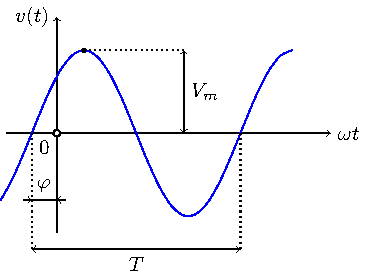
\includegraphics[width=0.8\linewidth]{teo_fig032.pdf}
       \caption{Haromincká funkce $v = V_m\cos(\omega t + \varphi)$ resp. 
                $v= V_m\cos(\omega t + \varphi')$ kde je $\varphi' = \varphi - \frac{T}{4}$}
       \label{teo:fig032}
    \end{figure}

    Střídavou veličinu $v$ lze též do jisté míry charakterizovat \emph{činitelem tvaru} $\beta$,
    \emph{činitelem výkyvu} $\gamma$ a \emph{činitelem plnění} $\alpha$ definovanými vztahy
    \begin{equation}\label{TEO:eq_harm07}
      \beta = \frac{V}{V_s}, \quad \gamma = \frac{V_m}{V}, \quad \alpha = \frac{V_s}{V_m}
    \end{equation}    
    Je zřejmé, že platí $\alpha\beta\gamma = 1$.
    
    V elektrotechnice mají velkou důležitost periodická napětí a proudy, jejichž závislost je dána
    sinusovou nebo kosinusovou funkcí, tj.
    \begin{equation}\label{TEO:eq_harm08}
      v = V_m\sin(\omega t + \varphi),
    \end{equation}        
    nebo
    \begin{equation}\label{TEO:eq_harm09}
      v = V_m\cos(\omega t + \varphi),
    \end{equation}  
    kde $V_m$, $\omega$, $\varphi$ jsou konstanty (obr. \ref{teo:fig032})
    
    Jelikož, tato napětí, resp. proudy představují \emph{harmonické kmity}, nazýváme je
    \emph{harmonicky proměnné}, nebo krátce \emph{harmonická napětí} resp. \emph{harmonická
    proudy}. Konstanta $V_m$ je maximální hodnota, či-li \emph{amplituda}, $\omega t + \varphi$ je
    \emph{fáze}, $\omega = 2\pi f = \frac{2\pi}{T}$ je \emph{úhlový kmitočet} a $\varphi$ je
    \emph{počáteční fáze} harmonické funkce.
    
    Rozdíl fází dvou harmonických veličin (stejného kmitočtu) nazýváme \emph{fázový posun}.
    
    % --------example: Efektivní hodnota výpočet -----------
    % \label{TEO:exam007}
    % !TeX spellcheck = cs_CZ
\begin{example}\label{TEO:exam007}
  Pro harmonickou veličinu, určete efektivní hodnotu, střední hodnotu, činitele tvaru, činitele
  výkyvu a činitele plnění \newline
  \textbf{Řešení:} Efektivní hodnota je:
  \begin{align}
    V &= \sqrt{\frac{1}{T}\int_0^TV_m^2\cos^2{(\omega t + \varphi)}\,dt}    \nonumber  \\
      &= \sqrt{\frac{1}{T}\int_0^TV_m^2\sin^2{(\omega t + \varphi)}\,dt} = 
         \frac{1}{\sqrt{2}}V_m \doteq 0.707 V_m   
  \end{align}
  Podrobný výpočet tohoto integrálu pomocí substituce $\omega t + \varphi=\dfrac{\alpha}{2}$ je
  poněkud zdlouhavější:
  \begin{align*}
      \omega t + \varphi=\dfrac{\alpha}{2}   
    & \rightarrow  2(\omega t + \varphi) = \alpha      \\ 
      \omega dt = \frac{1}{2}d\alpha         
    & \rightarrow dt = \frac{1}{2\omega}d\alpha
  \end{align*}
  Nesmíme zapomenout přepočítat meze $\alpha_d\lvert_{t=0}=2\varphi$ a $\alpha_h\lvert_{t=T} = 
  4\pi+2\varphi$ nového integrálu.
  \begin{align*}
    V^2  &= \frac{V_m}{2T\omega}\int_{\alpha_d}^{\alpha_h}\cos^2\frac{\alpha}{2}\,d\alpha    \\
         &= \frac{V_m}{4\pi}\int_{\alpha_d}^{\alpha_h}\frac{1+\cos\alpha}{2}\,d\alpha  
          = \frac{V_m}{4\pi}\left(\left.\frac{\alpha}{2}\right\rvert_{\alpha_d}^{\alpha_h}
          + \left.\frac{1}{2}\sin\alpha\right\rvert_{\alpha_d}^{\alpha_h}\right)             \\
         &= \frac{V_m}{4\pi}\left(2\pi+\varphi-\varphi 
          + \frac{1}{2}\sin(4\pi+2\varphi)
          - \frac{1}{2}\sin(2\varphi)\right) = \frac{V_m}{2}.  
  \end{align*}  
  Při zjednodušování integrálu je užito známého goniometrického vzorce \(\cos^2\dfrac{\alpha}{2} = 
  \dfrac{1+\cos\alpha}{2}\) a faktu \(\sin(x+2k\pi)=\sin x\)
  
  Střední hodnota kladné půlvlny je 
  \begin{align*}
    V_s &= \frac{2}{T}\int\limits_{-S\frac{T}{4}-
           \frac{\varphi}{\omega}}^{\frac{T}{4}-
           \frac{\varphi}{\omega}}{V_m\cos(\omega t +\varphi)}\,dt                            \\
        &= \frac{2}{T}\int\limits_{-\frac{\varphi}{\omega}}^{-\frac{T}{2}-
           \frac{\varphi}{\omega}}{V_m\sin(\omega t +\varphi)}\,dt                            \\
        &= \frac{2}{\pi}V_m \doteq 0,637V_m
  \end{align*}
  činitele tvaru, výkyvu a plnění jsou 
  \begin{align*}
    \beta  &=\frac{V}{V_s}   =\frac{\pi}{2\sqrt{2}}=1,111, \\ 
    \gamma &=\frac{V_m}{V}   =\sqrt{2}\doteq1.414,         \\
    \alpha &=\frac{V_s}{V_m} =\frac{2}{\pi}\doteq0,637 
  \end{align*}
\end{example}  
    %-------------------------------------------------------
      
 %--------------------------------------------------------------------------------------------------
  \section{Obvody s nastavitelnými parametry}
    V praxi se setkáváme s obvody, u nichž lze (spojitě nebo stupňovitě) nastavit odpor odporníku, 
    kapacitu kondenzátoru, vlastní nebo vzájemnou indukčnost cívek, amplitudu, fázi nebo kmitočet
    zdroje (napětí nebo proud). Nazveme je \emph{obvody s nastavitelnými parametry}.
 %--------------------------------------------------------------------------------------------------

%} % tikzset
%---------------------------------------------------------------------------------------------------
%========== Kapitola: Obvody s rozprostřenými parametry ===========================================
  % !TeX spellcheck = cs_CZ
%file: teo1ch03.tex
%===========Kapitola: Obvody s rozprostřenými parametry====================================
\setchaptertoc
\chapter{Obvody s rozprostřenými parametry}\label{teo:IchapIX}

%~~~~~~~~~~~~~~~~~~~~~~~~~~~~~~~~~~~~~~~~~~~~~~~~~~~~~~~~~~~~~~~~~~~~~~~~~~~~~~~~~~~~~~~~~~~~~~~~~~  
%=============== Seznam literatury ================================================================
  \printbibliography[title={Seznam literatury}, heading=bibliography]
}  % DEBUG was off
%--------------------------------------------------------------------------------------------------
%                                       /$$$$$$$$  /$$$$$$ 
%                                       | $$_____/ /$$__  $$
%                                       | $$      | $$  \__/
%                                       | $$$$$   |  $$$$$$ 
%                                       | $$__/    \____  $$
%                                       | $$       /$$  \ $$
%                                       | $$$$$$$$|  $$$$$$/
%                                       |________/ \______/                     
%--------------------------------------------------------------------------------------------------
\ifthenelse{ \equal{\DebugMode}{true} }{ % Debug mode ON
  % !TeX program = lualatex
% !TeX root = luaking.tex
% !TeX encoding = UTF-8
% !TeX spellcheck = cs_CZ
%=================== Kapitola: Bipolární tranzistory ==============================================
\setchaptertoc
\chapter{Bipolární tranzistory}\label{es:IchapV}
  \section{Všeobecné poznatky}\label{es:IchapVsecI}
    Tranzistor je polovodičový prvek určeny na zesilovaní nebo generovaní elektrických signálu,
    jedná se tedy o \emph{aktivní} součástku.

    Podle činnosti rozdělujeme tranzistory: 
    \begin{itemize}[noitemsep]
      \item s injekcí, které využívají majoritní i minoritní nosiče (bipolární),
      \item řízené polem, které využívají pouze majoritní nosiče náboje (unipolární).
    \end{itemize}
     
    Bipolámí tranzistory představují aktivní polovodičové prvky. Jsou tvořeny dvěma přechody PN,
    tzn. třemi vrstvami z rozdílně dotovaného polovodičového materiálu. Podle pořadí vrstev
    rozlišujeme dvě skupiny bipolárních tranzistorů, a to tranzistory \textsc{NPN} a tranzistory
    \textsc{PNP}. Obě uspořádání tranzistorů jsou znázorněna na obr. \ref{teo:fig053}, kde je
    zobrazeno jak pořadí vrstev, tak příslušná schematická značka.

    \begin{figure}[ht!]
      \centering  
      \subcaptionbox{\textsc{PNP}\label{teo:fig053a}}{\luafigure[0.3]{teo_fig053a.pdf}} \hspace{1em}
      \subcaptionbox{\textsc{NPN}\label{teo:fig053b}}{\luafigure[0.3]{teo_fig053b.pdf}} \\
      \subcaptionbox{\label{teo:fig053c}}{\luafigure[0.3]{teo_fig053c.pdf}}             \hspace{1em}
      \subcaptionbox{\label{teo:fig053d}}{\luafigure[0.3]{teo_fig053d.pdf}}                   
      \caption{Pořadí vrstev polovodiče a schematická značka bipolárních NPN a PNP 
      tranzistorů (\cite[s.~112]{Frohn2006})}
      \label{teo:fig053}
    \end{figure}
    
    Označení \uv{tranzistor} je uměle vytvořené slovo z anglických slov \textbf{tran}sfer = přenášet
    a re\textbf{zistor} = odpor. Označení \uv{bipolámí} (bi = dva) má poukázat na skutečnost, že je
    hlavní proud určen dvěma rozdílnými druhy nositelů náboje. Ve všeobecném povědomí se však pro
    bipolární tranzistor ustálil zjednodušený pojem tranzistor. Na rozdíl od bipolárních tranzistorů
    teče u unipolárních tranzistorů (unum = jeden) hlavní proud pouze jedinou oblastí a z toho
    vyplývá, že je určen pouze jediným typem nositele náboje podle toho, jakým způsobem byl dotován
    polovodičový materiál. Unipolární tranzistory často označujeme jako tranzistory řízené
    elektrickým polem. Jejich princip bude uveden v kapitole \ref{es:IchapVI}.
    
    Pro uživatele má velký význam znalost vlastností a chování jednotlivých typů tranzistorů. Proto
    výrobci ke každému typu tranzistoru vydávají katalogové listy, které obsahují charakteristické
    hodnoty, charakteristiky a mezní hodnoty (obdobně jako u diod).
    
    Protože tranzistor představuje dvojbran, jenž má dvě vstupní a dvě výstupní elektrody, je počet
    charakteristických hodnot a charakteristik podstatně větší než u polovodičových diod. Některé
    důležité parametry a charakteristiky budou blíže objasněny v následujících odstavcích.
    
    Bipolární tranzistory využívají jako výchozího materiálu nejčastěji křemíku, pro vysoké kmitočty
    se používají tranzistory ze sloučenin typu \(A^{III}B^{V}\).
    
    Tranzistory můžeme rozdělovat podle mnoha hledisek. Z hlediska konstrukce je zásadní rozdělení
    na tranzistory pro malé signály (nízkého výkonu) a výkonové tranzistory. Takovéto rozdělení
    podle konstrukce je uvedeno na obr. \ref{teo:fig073}.
    
    Tranzistory nízkého výkonu se převážně používají pro zesilování malých střídavých signálů.
    Tranzistory mají v tomto případě pevně nastavený klidový pracovní bod a přiváděné signálové
    napětí je malé, tzn. že nesmějí být příliš vybuzeny. Další oblastí použití tranzistorů nízkého
    výkonu jsou elektronické spínače, které jsou buzeny v celém možném rozsahu charakteristik.
    
    Výkonové tranzistory jsou dimenzovány na velké proudy a velká napětí. Mají proto relativně větší
    pouzdra, díky nimž je možné rychleji odvádět větší množství vznikajícího tepla z krystalu
    polovodiče. Výkonové tranzistory nalézají uplatnění v zesilovačích velkých signálů, tj.
    výkonových a koncových stupních nebo zastávají funkci elektronických spínačů.

    \begin{mdframed}[style=mdnote]
      \small
      Krátce po skončení války v roce 1945, Bellovy laboratoře vytvořily skupinu pro výzkum fyziky
      pevných látek, pod vedením \textsc{Shockleyho}. Jejich cílem bylo najít alternativu ke křehkým
      elektronkovým zesilovačům. Jejich první pokusy byly založeny na Shockleyově myšlence, že
      vnější elektrické pole na polovodiči ovlivní jeho vodivost. Jejich experimenty však záhadně
      selhávaly.

      Skupina začala studovat atomové struktury, které se na povrchu a uvnitř látek liší. Hledané
      výsledky se začaly dostavovat v okamžiku, když začali obklopovat body dotyku mezi polovodičem
      a přívodními vodiči elektrolytem. \textsc{Hilbert Moore} postavil okruh, který jim dovolil
      snadno měnit frekvenci vstupního signálu a navrhl, aby používali glykol boritan, viskózní
      chemikálii, která se nevypařovala. Nakonec získali důkaz schopnosti zesílení signálu, když
      fyzik \textsc{Gerald Pearson}, podle návrhu Shockleyho, uvedl napětí na kapičku glykol
      boritanu umístěnou přes \textsc{P-N} přechod. V prosinci 1947 Bardeen a Brattain - pracovali
      bez Shockleyho - uspěli ve stvoření hrotového tranzistoru, který zesiloval signál.

      Další měsíc začali patentoví zástupci Bellových laboratoří pracovat na patentových
      přihláškách. Brzo objevili, že Shockleyho vliv elektrického pole na polovodič byl předpovídán
      a patentován v roce 1930 \textsc{Juliem Lilienfeldem}, který si svůj \textsc{MESFET}
      patentoval v Kanadě již v 22. října 1925. Přesto byly podány celkem čtyři žádosti o patent. Na
      žádné z těchto přihlášek se však nevyskytovalo Shockleyovo jméno. To Shockleyho rozzlobilo,
      protože práce byla založena na jeho nápadu s účinkem elektrického pole. 
      
      Ve stejnou dobu tiše pokračoval ve vlastní práci na stavbě různých druhů tranzistoru
      založených na spojení místo bodového dotyku. Předpokládal, že tento typ tranzistoru bude více
      komerčně úspěšný. Shockley pracoval na \emph{teorii elektronů a děr v polovodičích}, která
      byla nakonec vydána jako 558 stránková monografie v roce 1950. V té Shockley vypracoval
      rozhodující myšlenky týkající se pohybu elektronů a děr a diferenciální rovnici, kterou se
      řídí tok elektronů v pevných krystalech.

      Shockleyho tato práce vedla k myšlence \emph{sendvičového tranzistoru} a ke vzniku klasického
      tranzistoru. Jeho objev byl oznámen 4. června 1951 a Shockley obdržel 25. září 1951 za jeho
      objev patent. Pro výrobu tohoto tranzistoru byla vyvinuta difúzní metoda a tento tranzistor
      brzy zastínil tranzistor s bodovými kontakty. Shockley pokračoval jako vedoucí skupiny v
      Bellových laboratořích ještě dva roky.

      {\centering
        \captionsetup{type=figure}
        \luafigure[1]{teo_fig071.png}
        \captionof{figure}{\textsc{John Bardeen}, \textsc{William Shockley} a \textsc{Walter Brattain} 
          v Bell Labs, 1948. (\cite[s.~6]{KolkaBiolek2011})
        \label{teo:fig071}}
      \par}

      V roce 1951 byl zvolen členem National Academy of Sciences (NAS). Za svůj objev tranzistoru
      získal mnoho cen. Bellovy laboratoře však představovaly všechny tři vynálezce (Shockleyho,
      Bardeena a Brattaina) jako tým. To vedlo k rozkolu a Shockley později blokoval práci Bardeena
      a Brattaina na klasickém tranzistoru.

      Shockley nakonec začal řídit svoji vlastní společnost, v níž se pokoušel vytvořit nové a
      technicky obtížné zařízení (původně nazvané čtyřvrstvá dioda a nyní známé jako tyristor).
      Projekt se ale rozvíjel velmi pomalu. 

      V roce 1956 Shockley získal, spolu s Bardeenem a Brattainem, Nobelovu cenu za fyziku. Ve své
      Nobelovské přednášce plně ocenil Brattaina a Bardeena jako vynálezce tranzistoru s bodovými
      kontakty.
    \end{mdframed}
    
    Pro lepší orientaci ve velkém množství vyráběných typů tranzistorů bylo zavedeno označovací
    schéma. Evropští výrobci používají hlavně značení \uv{Pro-Electron\footnote{Pro Electron nebo
    EECA je evropský typový a registrační systém pro aktivní komponenty (jako jsou polovodiče,
    displeje z tekutých krystalů, senzorová zařízení, elektronky a katodové trubice). Společnost Pro
    Electron byla založena v roce 1966 v belgickém Bruselu. V roce 1983 byla sloučena s Evropskou
    asociací výrobců elektronických součástek (EECA) a od té doby působí jako agentura EECA.}},
    které využívá kombinace písmen a číslic.

    \luagraphic[1]{teo_fig079.jpg}{Pohled na čip \textsc{MJ1000} v TO3 pouzdře. Čip obsahuje dva 
      tranzistory v Darlingtonovo zapojení. První, méně výkonný tranzistor se zesílením cca 100 
      budí druhý výkonový tranzistor se zesílením cca 10. Výsledný zesilovací činitel je dán 
      přibližně vynásobením zesilovacích činitelů obou tranzistorů (cca 1000).}{teo:fig079}

    Aby mohl tranzistor řádně pracovat, musí mít potřebné napětí nejen mezi kolektorem a emitorem,
    ale také dostatečně velké napětí mezi bází a emitorem. Velkou roli přitom hraje teplotní
    stabilizace klidového pracovního bodu. Je potřebná z toho důvodu, že při stoupající teplotě
    okolí narůstají též proudy, které tranzistorem protékají. Následkem zvyšování teploty se krystal
    ohřívá a roste tak jeho vodivost, čímž se příslušné proudy zvětšují. Tímto způsobem stoupá
    ztrátový výkon, tranzistor se proto více ohřívá atd. Na konci tohoto koloběhu je tepelná
    destrukce tranzistoru, který se tak stává nepoužitelným.

    \begin{figure*}
      \centering
      \luafigure[1]{teo_fig073.png}
      \caption{Druhy bipolárních tranzistorů podle konstrukce. (\cite[s.~115]{Frohn2006})}
      \label{teo:fig073}
    \end{figure*}

    Tranzistory mohou pracovat ve třech různých základních zapojeních - se společným emitorem
    (\textsc{SE}), se společným kolektorem (\textsc{SC}) a se společnou bází (\textsc{SB}). Zapojení
    je pojmenováno podle toho, která z elektrod je společná vstupu a výstupu zesilovacího stupně pro
    zesilování střídavých napětí, tj. která představuje společný pól signálového napětí na vstupu a
    na výstupu daného stupně. Každé z těchto základních zapojení má své přednosti a nedostatky.
    Nejčastěji se používá zapojení \textsc{SE}. Zapojení \textsc{SC} se používá jako měnič impedance
    (velká vstupní a malá výstupní impedance). Zapojení \textsc{SB} má svůj význam hlavně ve
    vysokofrekvenční technice, jinak představuje také měnič impedance, avšak s přesně opačným
    účinkem než předchozí zapojení (malá vstupní a velká výstupní impedance).

    Při praktickém využití musejí být tranzistory, a to ať se jedná o jakékoliv zapojení, doplněny
    dalšími součástkami. Zapojení těchto součástek (rezistorů a kondenzátorů) závisí na tom, jakou
    úlohu má zapojení s tranzistorem plnit. Musíme rozlišit, zda má tranzistor pracovat ve
    stejnosměrném zesilovači, v zesilovači střídavých napětí, ve výkonovém zesilovači nebo zda má
    mít funkci spínače.

    Stejnosměrné zesilovače se používají všude tam, kde je zapotřebí zesilovat stejnosměrná napětí a
    změny napětí od velmi malých až k vysokým frekvencím. Typickým představitelem je např. zesilovač
    Y osciloskopu. Aby stejnosměrné zesilovače mohly řádně plnit svou funkci, nesmějí obsahovat
    žádné součástky, které by ovlivňovaly jejich zesílení na různých frekvencích a neumožňovaly
    galvanickou vazbu (např. kondenzátory).

    Střídavé zesilovače mohou naproti tomu zesilovat střídavá napětí o frekvenci několika \si{\Hz}
    až do několika \si{\GHz} (podle typu tranzistoru a dimenzování zapojení), avšak nemusejí
    zesilovat stejnosměrná napětí. Důležitými prvky v těchto zesilovačích jsou kondenzátory.

    Výkonové zesilovače mají spotřebiči odevzdat pokud možno co největší signálový výkon. Spotřebič
    může být představován např. reproduktorem (nízkofrekvenční výkonový zesilovač), vysílací anténou
    (vysokofrekvenční výkonový zesilovač) nebo motorem (aplikace výkonového zesilovače v regulační
    technice). Na spínače jsou kladeny zcela jiné požadavky než na stejnosměrné nebo střídavé
    zesilovače. Spínače mají co nejrychleji přecházet ze stavu \uv{zapnuto} do stavu \uv{vypnuto} a
    naopak. V tomto případě hrají velkou roli parazitní kapacity tranzistorů.


  \section{Základní princip}\label{es:IchapVsecII}
    \subsection{Princip funkce NPN a PNP tranzistorů}\label{es:IchapVsecIIssecI}
      První tranzistory byly vyráběny legováním. Tato technologie byla převzata z výroby diod. Aby
      byly vyrobeny dva přechody, byly na obě strany dotovaného základního materiálu umístěny
      pilulky cizích prvků - donorů nebo akceptorů {obr. \ref{teo:fig072}. Při výrobním procesu pak
      cizí atomy z obou stran difundovaly do výchozího materiálu. Střední vrstva byla přitom velmi
      tenká a měla výrazně menší počet volných nositelů náboje než obě vnější vrstvy. Podle
      použitých výchozích materiálů a cizích prvků vznikl tranzistor NPN nebo PNP.

      \luagraphic[0.8]{teo_fig072.png}{Výroba tranzistoru NPN legováním.
        (\cite[s.~115]{Frohn2006})}{teo:fig072}
      
      Aby tranzistor fungoval, musí být mezi bázi a emitor připojen zdroj napětí tak, aby byl spodní
      přechod PN polarizován v propustném směru. Tranzistor NPN má proto bázi kladnější než emitor,
      tranzistor PNP má bázi zápornější než emitor. Napětí mezi bází a emitorem křemíkových
      tranzistorů má velikost \(U_{BE} \approx \SI{0.7}{\V}\), tj. stejné, jako je difuzní napětí
      křemíkových diod. Na obr. \ref{teo:fig074} a \ref{teo:fig075} zakreslené proudy vyznačují směr
      toku elektronů.

      \luagraphic[1]{teo_fig074.png}{Znázornění tranzistoru NPN. \(\longrightarrow\) udáva směr 
        toku elektronů). (\cite[s.~116]{Frohn2006})}{teo:fig074}
      
      Horní přechod PN pracuje v závěrném směru. Zdroje napětí jsou z tohoto důvodu zapojeny tak,
      aby byl kolektor u NPN tranzistoru kladnější než emitor, u PNP tranzistoru naopak zápornější
      než emitor.

      Vlivem připojených napětí bude spodní přechod PN zapojen v propustném směru a horní přechod PN
      v závěrném směru. Ve střední a horní oblasti se vytvoří závěrná vrstva. Ta se rozprostírá
      téměř po celé šířce střední oblasti, která je velmi tenká a obsahuje pouze malý počet nositelů
      náboje.        

      \luagraphic[1]{teo_fig075.png}{Znázornění tranzistoru PNP.  \(\longrightarrow\) udáva směr 
        toku elektronů). (\cite[s.~116]{Frohn2006})}{teo:fig075}
      
      Protože je spodní přechod PN zapojen v propustném směru, zaplavují nositelé náboje z emitoru
      závěrnou vrstvu ve střední oblasti. Tím se tato závěrná vrstva zmenší a její odpor klesne. Tím
      mohou nositelé náboje z emitoru projít zmenšenou závěrnou vrstvou do kolektorové oblasti a
      odtud odtéct k baterii (ke zdroji).

      Jelikož nositelé náboje pocházejí ze spodní oblasti, nazývá se tato oblast emitor. Střední
      oblast představuje výchozí bod pro oba přechody PN a nazývá se proto bází. Horní oblast
      shromažďuje všechny nositele náboje, které neodtekly bází a nese označení kolektor.

      \luagraphic[1]{teo_fig076.png}{Provozní napětí a proudy tranzistoru NPN. 
        (\cite[s.~117]{Frohn2006})}{teo:fig076}
      
      Proud \(l_B\), který odtéká vývodem báze, je podstatně menší než kolektorový proud \(l_C\),
      jenž protéká zmenšenou závěrnou vrstvou. Např. při napětí \(U_{BE} \approx \SI{0.7}{\V}\)
      protéká bází proud \(I_B = \SI{1}{\mA}\) a kolektorem proud \(I_C \approx \SI{100}{\mA}\).
      Jestliže nyní nepatrné zvětšíme \(U_{BE}\), vzroste proud báze např. na \(I_B = \SI{2}{\mA}\),
      čímž k závěrné vrstvě doputuje více nositelů náboje z emitoru. Tím se závěrná vrstva ještě
      více zmenší a kolektorový proud vzroste např. na \(I_C \approx \SI{200}{\mA}\). Naopak při
      zmenšení napětí \(U_{BE}\) a tím též proudu \(l_B\) se odpor závěrné vrstvy zvětší a
      kolektorový proud \(I_C\) klesne. Zjišťujeme, že proud báze \(l_B\) a proud kolektoru \(l_C\)
      tranzistoru se v širokém rozmezí mění proporcionálně. U tranzistoru je tak možné malým proudem
      báze \(l_B\), jenž představuje vstupní proud, řídit podstatně větší kolektorový proud \(l_C\),
      který je výstupním proudem. Tato souvislost se udává formou \emph{proudového zesílení
      nakrátko} \(\beta\).

      \begin{equation*}
        \beta = \dfrac{\Delta I_C}{\Delta I_B} \qquad \text{při (\(U_{CE} = 0\))}
      \end{equation*}
        
      \luagraphic[1]{teo_fig077.png}{Provozní napětí a proudy tranzistoru PNP. 
        (\cite[s.~117]{Frohn2006})}{teo:fig077}
      
      Tranzistory NPN a PNP se navzájem principiálně odlišují pořadím vrstev. Proto se odlišují též
      polaritou napětí \(U_{BE}\) a \(U_{CE}\). Obr. \ref {teo:fig076} a \ref {teo:fig077}
      vysvětluje souvislosti, které již byly naznačeny na obr. \ref{teo:fig074} a \ref{teo:fig075},
      tentokrát jsou ale použity schematické značky obou typů tranzistorů. Údaj napětí \(U_BE\) a
      \(U_{CE}\) je tvořen tak, že poslední písmeno udává vztažnou elektrodu, zde tedy emitor E. Při
      určování směru toku proudu vycházíme z technické orientace, jež je obvyklá (proud teče obvodem
      směrem od kladného k zápornému pólu zdroje). Všechny proudy, které tečou do tranzistoru, jsou
      kladné, vytékající proudy mají záporné znaménko.

      Aby byl tranzistor schopen činnosti, musí být vždy přechod báze-emitor v propustném směru a
      přechod báze-kolektor v závěrném směru.

      Na obr. \ref{teo:fig078a} je mezi vývod kolektoru a baterii zařazen ještě kolektorový rezistor
      \(R_C\), který plní funkci pracovního odporu. Ten omezuje proudové zesílení tranzistoru a
      přeměňuje je v napěťové zesílení. Tranzistor a kolektorový rezistor v tomto případě tvoří
      napěťový dělič pro napájecí napětí \(U_{CC} = \SI{+10}{\V}\). Při \(I_C = \SI{5}{\mA}\) a
      \(R_C = \SI{1}{\kohm}\) vzniká na kolektorovém rezistoru úbytek napětí
      \begin{equation*}
        U_{RC} = \SI{5e-3}{\mA}\cdot\SI{1}{\kohm} = \SI{5}{\V}
      \end{equation*}

      \luagraphic[1]{teo_fig078a.jpg}{apěťové zesílení tranzistoru NPN. 
        (\cite[s.~117]{Frohn2006})}{teo:fig078a}

      Napětí kolektor-emitor tranzistoru, které představuje výstupní napětí, bude 
      \begin{equation*}
        U_{CE} = U_{CC} - U_{RC} = \SI{10}{\V} - \SI{5}{\V} = \SI{5}{\V}
      \end{equation*}
      Jestliže se napětí \(U_{BE}\) vlivem střídavého napětí z připojeného generátoru v daný okamžik
      zvětší např. na \(U_{BE} = \SI{0.71}{\V}\), vzroste proud báze, který způsobí zvětšení
      kolektorového proudu, který, dejme tomu, vzroste z \(I_C = \SI{5}{\mA}\) na \(I_C =
      \SI{6.5}{\mA}\). Tento zvětšený kolektorový proud vyvolá na kolektorovém rezistoru zvětšený
      úbytek napětí
      \begin{equation*}
        U_{RC} = I_C\cdot R_C = \SI{6.5}{\mA}\cdot\SI{1}{\kohm} = \SI{6.5}{\V}
      \end{equation*}
      Tím napětí \(U_{CE}\) klesne na hodnotu \(U_{CE} = \SI{3.5}{\V}\). Při záporné půlvlně napětí
      generátoru se proud báze \(I_B\) zmenší, čímž se zmenši i proud kolektoru \(l_C\) a tím i
      úbytek napětí na kolektorovém rezistoru \(U_{RC}\). Důsledkem tohoto děje je zvětšení
      \(l_{CE}\) tranzistoru. Příslušné časové průběhy na obr. \ref{teo:fig078}. Generátor,
      připojený na bázi tranzistoru, způsobí změnu proudu báze \(\Delta I_B = \SI{20}{\micro\A}\),
      která vyvolá změnu kolektorového proudu \(\Delta I_C = \SI{3}{\mA}\).

      \begin{figure}[ht!]  %\ref{teo:fig078} 
        \centering
        \subcaptionbox{\(U_{BE}(t)\)\label{teo:fig078b}}{\luafigure[0.9]{teo_fig078b.jpg}}  \\                                                       
        \subcaptionbox{\(I_{B}(t)\) \label{teo:fig078c}}{\luafigure[0.9]{teo_fig078c.jpg}}  \\                  
        \subcaptionbox{\(I_{C}(t)\) \label{teo:fig078d}}{\luafigure[0.9]{teo_fig078d.jpg}}  \\                 
        \subcaptionbox{\(U_{RC}(t)\)\label{teo:fig078e}}{\luafigure[0.9]{teo_fig078e.jpg}}  \\                  
        \subcaptionbox{\(U_{CE}(t)\)\label{teo:fig078f}}{\luafigure[0.9]{teo_fig078f.jpg}}  \\                   
        \caption{Napěťové zesílení tranzistoru zapojeného podle obr. \ref{teo:fig078a} 
          (\cite[s.~118]{Frohn2006})}
        \label{teo:fig078}
      \end{figure}

      Odtud pro uvedený případ zjistíme \emph{proudové zesílení} tranzistoru
      \begin{equation*}
        \beta = \dfrac{\Delta I_C}{\Delta I_B} = \dfrac{\num{3e-3}}{\num{20e-6}} = 150
      \end{equation*}
      \emph{Napěťové zesílení} \(A_u\) zapojení s tranzistorem je definováno podobně jako proudové
      zesílení.
      \begin{equation*}
        A_u = \dfrac{\Delta U_{out}}{\Delta U_{in}} = \dfrac{\Delta U_{CE}}{\Delta U_{BE}}
      \end{equation*}
      Napěťové zesílení závisí kromě proudového zesílení také na velikosti kolektorového rezistoru
      \(R_C\). V příkladu způsobí vstupní střídavé napětí \(\Delta U_{BE} = \SI{-0.02}{\V}\) změnu
      výstupního střídavého napětí \(U_{CE} = \SI{-3}{\V}\). V tomto případě je tedy napěťové
      zesílení
      \begin{equation*}
        A_u = \dfrac{\Delta U_{CE}}{\Delta U_{BE}} = \dfrac{\num{-3}}{\num{0.02}} = -150
      \end{equation*}
      Pomocí kolektorového rezistoru \(R_{C}\) se změnilo proudové zesílení na napěťové zesílení
      tranzistoru. Znaménko \uv{-} naznačuje, že kladné půlvlně vstupního napětí odpovídá záporná
      půlvlna výstupního napětí.

  \section{Základní zapojení tranzistoru}\label{es:IchapVsecIII}
%---------------------------------------------------------------------------------------------------
}{ % DEBUG was off
\LuaPartBckgrnd{titleBG_fractal1.png}
\LuaPartTitle{ES I}{Elektronické součástky}{ESI}
\parttoc
%========== Kapitola: Pasivni součástky ==========================================================
  % !TeX spellcheck = cs_CZ
% file: kap_optocoupler.tex
%{\tikzset{external/prefix={tikz/TEO/}}
% \tikzset{external/figure name/.add={ch12_}{}}
%=================== Kapitola: Optoelektronika =====================================================
\setchaptertoc
\chapter{Pasivní elektronické součáskty}\label{teo:IchapXII}


  \section{Teplotní závislost pasivních prvků}\label{teo:IchapXIIsecI}
    
    \begin{example}\label{teo:exam001}
      Uvažujeme žárovku \SI{100}{\watt}, \SI{230}{\volt} s wolframovým vláknem s teplotním 
      součinitelem odporu \(\alpha = \SI{4.8e-3}{\per\kelvin}\).  Problematické je určení provozní 
      teploty vlákna. Vzhledem k tomu, že wolfram taje při teplotě \SI{3387}{\degreeCelsius} a 
      vlákno svítí bílým žárem, odhadneme teplotu na \SI{2500}{\degreeCelsius}. Ze vztahu \(P = 
      U^2/R\) určíme odpor vlákna: \(R = 230^2/100 = \SI{529}{\ohm}\). Odpor při pokojové teplotě 
      bude: 
      \(R_{20}=529/(1+\num{4.8e-3}\cdot2480) = \SI{41}{\ohm}\). 
      \begin{figure}[ht!]  %\ref{teo:fig018}
        \centering
        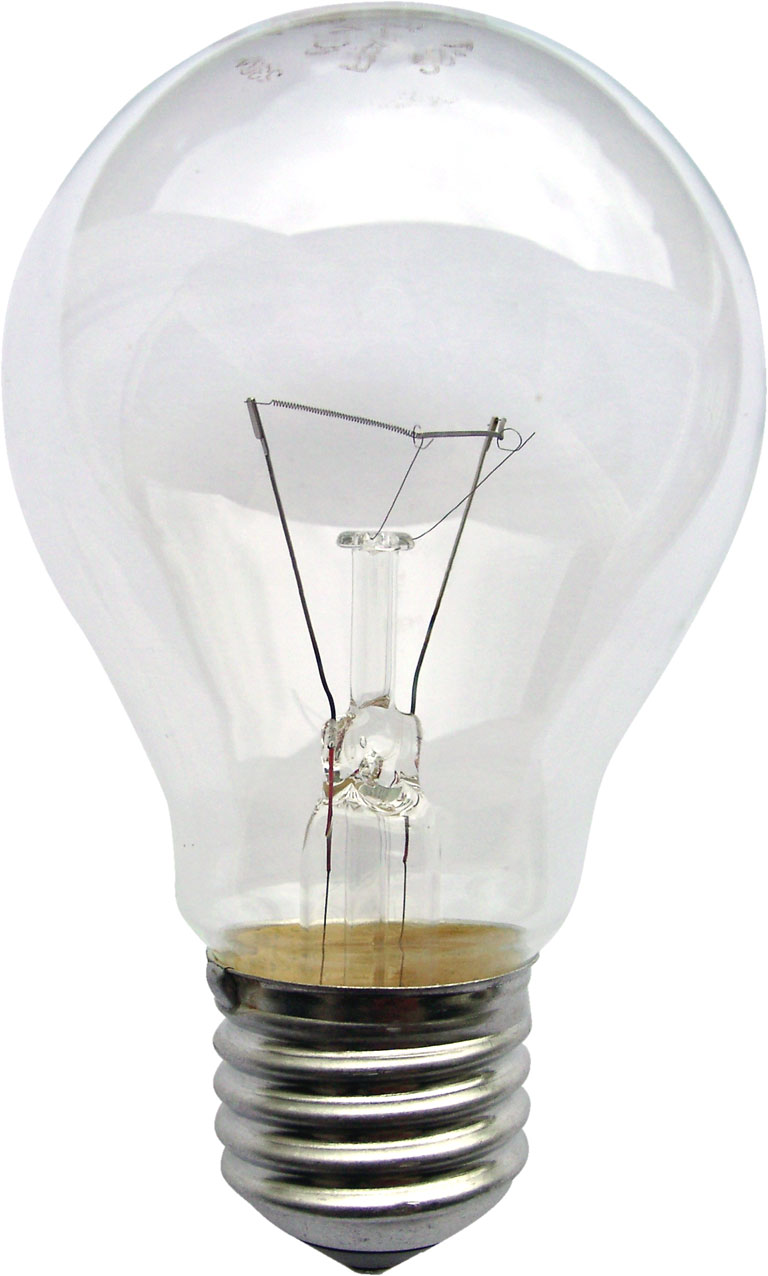
\includegraphics[width=0.3\linewidth]{teo_fig018.jpg}
        \caption{Žárovka jednoduchým způsobem přeměňuje elektrickou energii na světlo, zahříváním 
        tenkého wolframového vodiče průchodem elektrického proudu.}
        \label{teo:fig018}
      \end{figure}
      Podle tohoto přibližného výpočtu se zmenší odpor vlákna  téměř třináctkrát a odpovídajícím 
      způsobem vzrůstá i nárazový proud při zapnutí obvodu oproti ustálenému stavu. Z tohoto 
      pohledu měly původní Edisonovy uhlíkové žárovky lepší vlastnosti, protože teplotní součinitel 
      uhlíku je záporný (\cite[s.~84]{Lanicek1998}).
    \end{example}
%} % tikzset
%---------------------------------------------------------------------------------------------------
%========== Kapitola: Bipolární transzistory =====================================================
  % !TeX program = lualatex
% !TeX root = luaking.tex
% !TeX encoding = UTF-8
% !TeX spellcheck = cs_CZ
%=================== Kapitola: Bipolární tranzistory ==============================================
\setchaptertoc
\chapter{Bipolární tranzistory}\label{es:IchapV}
  \section{Všeobecné poznatky}\label{es:IchapVsecI}
    Tranzistor je polovodičový prvek určeny na zesilovaní nebo generovaní elektrických signálu,
    jedná se tedy o \emph{aktivní} součástku.

    Podle činnosti rozdělujeme tranzistory: 
    \begin{itemize}[noitemsep]
      \item s injekcí, které využívají majoritní i minoritní nosiče (bipolární),
      \item řízené polem, které využívají pouze majoritní nosiče náboje (unipolární).
    \end{itemize}
     
    Bipolámí tranzistory představují aktivní polovodičové prvky. Jsou tvořeny dvěma přechody PN,
    tzn. třemi vrstvami z rozdílně dotovaného polovodičového materiálu. Podle pořadí vrstev
    rozlišujeme dvě skupiny bipolárních tranzistorů, a to tranzistory \textsc{NPN} a tranzistory
    \textsc{PNP}. Obě uspořádání tranzistorů jsou znázorněna na obr. \ref{teo:fig053}, kde je
    zobrazeno jak pořadí vrstev, tak příslušná schematická značka.

    \begin{figure}[ht!]
      \centering  
      \subcaptionbox{\textsc{PNP}\label{teo:fig053a}}{\luafigure[0.3]{teo_fig053a.pdf}} \hspace{1em}
      \subcaptionbox{\textsc{NPN}\label{teo:fig053b}}{\luafigure[0.3]{teo_fig053b.pdf}} \\
      \subcaptionbox{\label{teo:fig053c}}{\luafigure[0.3]{teo_fig053c.pdf}}             \hspace{1em}
      \subcaptionbox{\label{teo:fig053d}}{\luafigure[0.3]{teo_fig053d.pdf}}                   
      \caption{Pořadí vrstev polovodiče a schematická značka bipolárních NPN a PNP 
      tranzistorů (\cite[s.~112]{Frohn2006})}
      \label{teo:fig053}
    \end{figure}
    
    Označení \uv{tranzistor} je uměle vytvořené slovo z anglických slov \textbf{tran}sfer = přenášet
    a re\textbf{zistor} = odpor. Označení \uv{bipolámí} (bi = dva) má poukázat na skutečnost, že je
    hlavní proud určen dvěma rozdílnými druhy nositelů náboje. Ve všeobecném povědomí se však pro
    bipolární tranzistor ustálil zjednodušený pojem tranzistor. Na rozdíl od bipolárních tranzistorů
    teče u unipolárních tranzistorů (unum = jeden) hlavní proud pouze jedinou oblastí a z toho
    vyplývá, že je určen pouze jediným typem nositele náboje podle toho, jakým způsobem byl dotován
    polovodičový materiál. Unipolární tranzistory často označujeme jako tranzistory řízené
    elektrickým polem. Jejich princip bude uveden v kapitole \ref{es:IchapVI}.
    
    Pro uživatele má velký význam znalost vlastností a chování jednotlivých typů tranzistorů. Proto
    výrobci ke každému typu tranzistoru vydávají katalogové listy, které obsahují charakteristické
    hodnoty, charakteristiky a mezní hodnoty (obdobně jako u diod).
    
    Protože tranzistor představuje dvojbran, jenž má dvě vstupní a dvě výstupní elektrody, je počet
    charakteristických hodnot a charakteristik podstatně větší než u polovodičových diod. Některé
    důležité parametry a charakteristiky budou blíže objasněny v následujících odstavcích.
    
    Bipolární tranzistory využívají jako výchozího materiálu nejčastěji křemíku, pro vysoké kmitočty
    se používají tranzistory ze sloučenin typu \(A^{III}B^{V}\).
    
    Tranzistory můžeme rozdělovat podle mnoha hledisek. Z hlediska konstrukce je zásadní rozdělení
    na tranzistory pro malé signály (nízkého výkonu) a výkonové tranzistory. Takovéto rozdělení
    podle konstrukce je uvedeno na obr. \ref{teo:fig073}.
    
    Tranzistory nízkého výkonu se převážně používají pro zesilování malých střídavých signálů.
    Tranzistory mají v tomto případě pevně nastavený klidový pracovní bod a přiváděné signálové
    napětí je malé, tzn. že nesmějí být příliš vybuzeny. Další oblastí použití tranzistorů nízkého
    výkonu jsou elektronické spínače, které jsou buzeny v celém možném rozsahu charakteristik.
    
    Výkonové tranzistory jsou dimenzovány na velké proudy a velká napětí. Mají proto relativně větší
    pouzdra, díky nimž je možné rychleji odvádět větší množství vznikajícího tepla z krystalu
    polovodiče. Výkonové tranzistory nalézají uplatnění v zesilovačích velkých signálů, tj.
    výkonových a koncových stupních nebo zastávají funkci elektronických spínačů.

    \begin{mdframed}[style=mdnote]
      \small
      Krátce po skončení války v roce 1945, Bellovy laboratoře vytvořily skupinu pro výzkum fyziky
      pevných látek, pod vedením \textsc{Shockleyho}. Jejich cílem bylo najít alternativu ke křehkým
      elektronkovým zesilovačům. Jejich první pokusy byly založeny na Shockleyově myšlence, že
      vnější elektrické pole na polovodiči ovlivní jeho vodivost. Jejich experimenty však záhadně
      selhávaly.

      Skupina začala studovat atomové struktury, které se na povrchu a uvnitř látek liší. Hledané
      výsledky se začaly dostavovat v okamžiku, když začali obklopovat body dotyku mezi polovodičem
      a přívodními vodiči elektrolytem. \textsc{Hilbert Moore} postavil okruh, který jim dovolil
      snadno měnit frekvenci vstupního signálu a navrhl, aby používali glykol boritan, viskózní
      chemikálii, která se nevypařovala. Nakonec získali důkaz schopnosti zesílení signálu, když
      fyzik \textsc{Gerald Pearson}, podle návrhu Shockleyho, uvedl napětí na kapičku glykol
      boritanu umístěnou přes \textsc{P-N} přechod. V prosinci 1947 Bardeen a Brattain - pracovali
      bez Shockleyho - uspěli ve stvoření hrotového tranzistoru, který zesiloval signál.

      Další měsíc začali patentoví zástupci Bellových laboratoří pracovat na patentových
      přihláškách. Brzo objevili, že Shockleyho vliv elektrického pole na polovodič byl předpovídán
      a patentován v roce 1930 \textsc{Juliem Lilienfeldem}, který si svůj \textsc{MESFET}
      patentoval v Kanadě již v 22. října 1925. Přesto byly podány celkem čtyři žádosti o patent. Na
      žádné z těchto přihlášek se však nevyskytovalo Shockleyovo jméno. To Shockleyho rozzlobilo,
      protože práce byla založena na jeho nápadu s účinkem elektrického pole. 
      
      Ve stejnou dobu tiše pokračoval ve vlastní práci na stavbě různých druhů tranzistoru
      založených na spojení místo bodového dotyku. Předpokládal, že tento typ tranzistoru bude více
      komerčně úspěšný. Shockley pracoval na \emph{teorii elektronů a děr v polovodičích}, která
      byla nakonec vydána jako 558 stránková monografie v roce 1950. V té Shockley vypracoval
      rozhodující myšlenky týkající se pohybu elektronů a děr a diferenciální rovnici, kterou se
      řídí tok elektronů v pevných krystalech.

      Shockleyho tato práce vedla k myšlence \emph{sendvičového tranzistoru} a ke vzniku klasického
      tranzistoru. Jeho objev byl oznámen 4. června 1951 a Shockley obdržel 25. září 1951 za jeho
      objev patent. Pro výrobu tohoto tranzistoru byla vyvinuta difúzní metoda a tento tranzistor
      brzy zastínil tranzistor s bodovými kontakty. Shockley pokračoval jako vedoucí skupiny v
      Bellových laboratořích ještě dva roky.

      {\centering
        \captionsetup{type=figure}
        \luafigure[1]{teo_fig071.png}
        \captionof{figure}{\textsc{John Bardeen}, \textsc{William Shockley} a \textsc{Walter Brattain} 
          v Bell Labs, 1948. (\cite[s.~6]{KolkaBiolek2011})
        \label{teo:fig071}}
      \par}

      V roce 1951 byl zvolen členem National Academy of Sciences (NAS). Za svůj objev tranzistoru
      získal mnoho cen. Bellovy laboratoře však představovaly všechny tři vynálezce (Shockleyho,
      Bardeena a Brattaina) jako tým. To vedlo k rozkolu a Shockley později blokoval práci Bardeena
      a Brattaina na klasickém tranzistoru.

      Shockley nakonec začal řídit svoji vlastní společnost, v níž se pokoušel vytvořit nové a
      technicky obtížné zařízení (původně nazvané čtyřvrstvá dioda a nyní známé jako tyristor).
      Projekt se ale rozvíjel velmi pomalu. 

      V roce 1956 Shockley získal, spolu s Bardeenem a Brattainem, Nobelovu cenu za fyziku. Ve své
      Nobelovské přednášce plně ocenil Brattaina a Bardeena jako vynálezce tranzistoru s bodovými
      kontakty.
    \end{mdframed}
    
    Pro lepší orientaci ve velkém množství vyráběných typů tranzistorů bylo zavedeno označovací
    schéma. Evropští výrobci používají hlavně značení \uv{Pro-Electron\footnote{Pro Electron nebo
    EECA je evropský typový a registrační systém pro aktivní komponenty (jako jsou polovodiče,
    displeje z tekutých krystalů, senzorová zařízení, elektronky a katodové trubice). Společnost Pro
    Electron byla založena v roce 1966 v belgickém Bruselu. V roce 1983 byla sloučena s Evropskou
    asociací výrobců elektronických součástek (EECA) a od té doby působí jako agentura EECA.}},
    které využívá kombinace písmen a číslic.

    \luagraphic[1]{teo_fig079.jpg}{Pohled na čip \textsc{MJ1000} v TO3 pouzdře. Čip obsahuje dva 
      tranzistory v Darlingtonovo zapojení. První, méně výkonný tranzistor se zesílením cca 100 
      budí druhý výkonový tranzistor se zesílením cca 10. Výsledný zesilovací činitel je dán 
      přibližně vynásobením zesilovacích činitelů obou tranzistorů (cca 1000).}{teo:fig079}

    Aby mohl tranzistor řádně pracovat, musí mít potřebné napětí nejen mezi kolektorem a emitorem,
    ale také dostatečně velké napětí mezi bází a emitorem. Velkou roli přitom hraje teplotní
    stabilizace klidového pracovního bodu. Je potřebná z toho důvodu, že při stoupající teplotě
    okolí narůstají též proudy, které tranzistorem protékají. Následkem zvyšování teploty se krystal
    ohřívá a roste tak jeho vodivost, čímž se příslušné proudy zvětšují. Tímto způsobem stoupá
    ztrátový výkon, tranzistor se proto více ohřívá atd. Na konci tohoto koloběhu je tepelná
    destrukce tranzistoru, který se tak stává nepoužitelným.

    \begin{figure*}
      \centering
      \luafigure[1]{teo_fig073.png}
      \caption{Druhy bipolárních tranzistorů podle konstrukce. (\cite[s.~115]{Frohn2006})}
      \label{teo:fig073}
    \end{figure*}

    Tranzistory mohou pracovat ve třech různých základních zapojeních - se společným emitorem
    (\textsc{SE}), se společným kolektorem (\textsc{SC}) a se společnou bází (\textsc{SB}). Zapojení
    je pojmenováno podle toho, která z elektrod je společná vstupu a výstupu zesilovacího stupně pro
    zesilování střídavých napětí, tj. která představuje společný pól signálového napětí na vstupu a
    na výstupu daného stupně. Každé z těchto základních zapojení má své přednosti a nedostatky.
    Nejčastěji se používá zapojení \textsc{SE}. Zapojení \textsc{SC} se používá jako měnič impedance
    (velká vstupní a malá výstupní impedance). Zapojení \textsc{SB} má svůj význam hlavně ve
    vysokofrekvenční technice, jinak představuje také měnič impedance, avšak s přesně opačným
    účinkem než předchozí zapojení (malá vstupní a velká výstupní impedance).

    Při praktickém využití musejí být tranzistory, a to ať se jedná o jakékoliv zapojení, doplněny
    dalšími součástkami. Zapojení těchto součástek (rezistorů a kondenzátorů) závisí na tom, jakou
    úlohu má zapojení s tranzistorem plnit. Musíme rozlišit, zda má tranzistor pracovat ve
    stejnosměrném zesilovači, v zesilovači střídavých napětí, ve výkonovém zesilovači nebo zda má
    mít funkci spínače.

    Stejnosměrné zesilovače se používají všude tam, kde je zapotřebí zesilovat stejnosměrná napětí a
    změny napětí od velmi malých až k vysokým frekvencím. Typickým představitelem je např. zesilovač
    Y osciloskopu. Aby stejnosměrné zesilovače mohly řádně plnit svou funkci, nesmějí obsahovat
    žádné součástky, které by ovlivňovaly jejich zesílení na různých frekvencích a neumožňovaly
    galvanickou vazbu (např. kondenzátory).

    Střídavé zesilovače mohou naproti tomu zesilovat střídavá napětí o frekvenci několika \si{\Hz}
    až do několika \si{\GHz} (podle typu tranzistoru a dimenzování zapojení), avšak nemusejí
    zesilovat stejnosměrná napětí. Důležitými prvky v těchto zesilovačích jsou kondenzátory.

    Výkonové zesilovače mají spotřebiči odevzdat pokud možno co největší signálový výkon. Spotřebič
    může být představován např. reproduktorem (nízkofrekvenční výkonový zesilovač), vysílací anténou
    (vysokofrekvenční výkonový zesilovač) nebo motorem (aplikace výkonového zesilovače v regulační
    technice). Na spínače jsou kladeny zcela jiné požadavky než na stejnosměrné nebo střídavé
    zesilovače. Spínače mají co nejrychleji přecházet ze stavu \uv{zapnuto} do stavu \uv{vypnuto} a
    naopak. V tomto případě hrají velkou roli parazitní kapacity tranzistorů.


  \section{Základní princip}\label{es:IchapVsecII}
    \subsection{Princip funkce NPN a PNP tranzistorů}\label{es:IchapVsecIIssecI}
      První tranzistory byly vyráběny legováním. Tato technologie byla převzata z výroby diod. Aby
      byly vyrobeny dva přechody, byly na obě strany dotovaného základního materiálu umístěny
      pilulky cizích prvků - donorů nebo akceptorů {obr. \ref{teo:fig072}. Při výrobním procesu pak
      cizí atomy z obou stran difundovaly do výchozího materiálu. Střední vrstva byla přitom velmi
      tenká a měla výrazně menší počet volných nositelů náboje než obě vnější vrstvy. Podle
      použitých výchozích materiálů a cizích prvků vznikl tranzistor NPN nebo PNP.

      \luagraphic[0.8]{teo_fig072.png}{Výroba tranzistoru NPN legováním.
        (\cite[s.~115]{Frohn2006})}{teo:fig072}
      
      Aby tranzistor fungoval, musí být mezi bázi a emitor připojen zdroj napětí tak, aby byl spodní
      přechod PN polarizován v propustném směru. Tranzistor NPN má proto bázi kladnější než emitor,
      tranzistor PNP má bázi zápornější než emitor. Napětí mezi bází a emitorem křemíkových
      tranzistorů má velikost \(U_{BE} \approx \SI{0.7}{\V}\), tj. stejné, jako je difuzní napětí
      křemíkových diod. Na obr. \ref{teo:fig074} a \ref{teo:fig075} zakreslené proudy vyznačují směr
      toku elektronů.

      \luagraphic[1]{teo_fig074.png}{Znázornění tranzistoru NPN. \(\longrightarrow\) udáva směr 
        toku elektronů). (\cite[s.~116]{Frohn2006})}{teo:fig074}
      
      Horní přechod PN pracuje v závěrném směru. Zdroje napětí jsou z tohoto důvodu zapojeny tak,
      aby byl kolektor u NPN tranzistoru kladnější než emitor, u PNP tranzistoru naopak zápornější
      než emitor.

      Vlivem připojených napětí bude spodní přechod PN zapojen v propustném směru a horní přechod PN
      v závěrném směru. Ve střední a horní oblasti se vytvoří závěrná vrstva. Ta se rozprostírá
      téměř po celé šířce střední oblasti, která je velmi tenká a obsahuje pouze malý počet nositelů
      náboje.        

      \luagraphic[1]{teo_fig075.png}{Znázornění tranzistoru PNP.  \(\longrightarrow\) udáva směr 
        toku elektronů). (\cite[s.~116]{Frohn2006})}{teo:fig075}
      
      Protože je spodní přechod PN zapojen v propustném směru, zaplavují nositelé náboje z emitoru
      závěrnou vrstvu ve střední oblasti. Tím se tato závěrná vrstva zmenší a její odpor klesne. Tím
      mohou nositelé náboje z emitoru projít zmenšenou závěrnou vrstvou do kolektorové oblasti a
      odtud odtéct k baterii (ke zdroji).

      Jelikož nositelé náboje pocházejí ze spodní oblasti, nazývá se tato oblast emitor. Střední
      oblast představuje výchozí bod pro oba přechody PN a nazývá se proto bází. Horní oblast
      shromažďuje všechny nositele náboje, které neodtekly bází a nese označení kolektor.

      \luagraphic[1]{teo_fig076.png}{Provozní napětí a proudy tranzistoru NPN. 
        (\cite[s.~117]{Frohn2006})}{teo:fig076}
      
      Proud \(l_B\), který odtéká vývodem báze, je podstatně menší než kolektorový proud \(l_C\),
      jenž protéká zmenšenou závěrnou vrstvou. Např. při napětí \(U_{BE} \approx \SI{0.7}{\V}\)
      protéká bází proud \(I_B = \SI{1}{\mA}\) a kolektorem proud \(I_C \approx \SI{100}{\mA}\).
      Jestliže nyní nepatrné zvětšíme \(U_{BE}\), vzroste proud báze např. na \(I_B = \SI{2}{\mA}\),
      čímž k závěrné vrstvě doputuje více nositelů náboje z emitoru. Tím se závěrná vrstva ještě
      více zmenší a kolektorový proud vzroste např. na \(I_C \approx \SI{200}{\mA}\). Naopak při
      zmenšení napětí \(U_{BE}\) a tím též proudu \(l_B\) se odpor závěrné vrstvy zvětší a
      kolektorový proud \(I_C\) klesne. Zjišťujeme, že proud báze \(l_B\) a proud kolektoru \(l_C\)
      tranzistoru se v širokém rozmezí mění proporcionálně. U tranzistoru je tak možné malým proudem
      báze \(l_B\), jenž představuje vstupní proud, řídit podstatně větší kolektorový proud \(l_C\),
      který je výstupním proudem. Tato souvislost se udává formou \emph{proudového zesílení
      nakrátko} \(\beta\).

      \begin{equation*}
        \beta = \dfrac{\Delta I_C}{\Delta I_B} \qquad \text{při (\(U_{CE} = 0\))}
      \end{equation*}
        
      \luagraphic[1]{teo_fig077.png}{Provozní napětí a proudy tranzistoru PNP. 
        (\cite[s.~117]{Frohn2006})}{teo:fig077}
      
      Tranzistory NPN a PNP se navzájem principiálně odlišují pořadím vrstev. Proto se odlišují též
      polaritou napětí \(U_{BE}\) a \(U_{CE}\). Obr. \ref {teo:fig076} a \ref {teo:fig077}
      vysvětluje souvislosti, které již byly naznačeny na obr. \ref{teo:fig074} a \ref{teo:fig075},
      tentokrát jsou ale použity schematické značky obou typů tranzistorů. Údaj napětí \(U_BE\) a
      \(U_{CE}\) je tvořen tak, že poslední písmeno udává vztažnou elektrodu, zde tedy emitor E. Při
      určování směru toku proudu vycházíme z technické orientace, jež je obvyklá (proud teče obvodem
      směrem od kladného k zápornému pólu zdroje). Všechny proudy, které tečou do tranzistoru, jsou
      kladné, vytékající proudy mají záporné znaménko.

      Aby byl tranzistor schopen činnosti, musí být vždy přechod báze-emitor v propustném směru a
      přechod báze-kolektor v závěrném směru.

      Na obr. \ref{teo:fig078a} je mezi vývod kolektoru a baterii zařazen ještě kolektorový rezistor
      \(R_C\), který plní funkci pracovního odporu. Ten omezuje proudové zesílení tranzistoru a
      přeměňuje je v napěťové zesílení. Tranzistor a kolektorový rezistor v tomto případě tvoří
      napěťový dělič pro napájecí napětí \(U_{CC} = \SI{+10}{\V}\). Při \(I_C = \SI{5}{\mA}\) a
      \(R_C = \SI{1}{\kohm}\) vzniká na kolektorovém rezistoru úbytek napětí
      \begin{equation*}
        U_{RC} = \SI{5e-3}{\mA}\cdot\SI{1}{\kohm} = \SI{5}{\V}
      \end{equation*}

      \luagraphic[1]{teo_fig078a.jpg}{apěťové zesílení tranzistoru NPN. 
        (\cite[s.~117]{Frohn2006})}{teo:fig078a}

      Napětí kolektor-emitor tranzistoru, které představuje výstupní napětí, bude 
      \begin{equation*}
        U_{CE} = U_{CC} - U_{RC} = \SI{10}{\V} - \SI{5}{\V} = \SI{5}{\V}
      \end{equation*}
      Jestliže se napětí \(U_{BE}\) vlivem střídavého napětí z připojeného generátoru v daný okamžik
      zvětší např. na \(U_{BE} = \SI{0.71}{\V}\), vzroste proud báze, který způsobí zvětšení
      kolektorového proudu, který, dejme tomu, vzroste z \(I_C = \SI{5}{\mA}\) na \(I_C =
      \SI{6.5}{\mA}\). Tento zvětšený kolektorový proud vyvolá na kolektorovém rezistoru zvětšený
      úbytek napětí
      \begin{equation*}
        U_{RC} = I_C\cdot R_C = \SI{6.5}{\mA}\cdot\SI{1}{\kohm} = \SI{6.5}{\V}
      \end{equation*}
      Tím napětí \(U_{CE}\) klesne na hodnotu \(U_{CE} = \SI{3.5}{\V}\). Při záporné půlvlně napětí
      generátoru se proud báze \(I_B\) zmenší, čímž se zmenši i proud kolektoru \(l_C\) a tím i
      úbytek napětí na kolektorovém rezistoru \(U_{RC}\). Důsledkem tohoto děje je zvětšení
      \(l_{CE}\) tranzistoru. Příslušné časové průběhy na obr. \ref{teo:fig078}. Generátor,
      připojený na bázi tranzistoru, způsobí změnu proudu báze \(\Delta I_B = \SI{20}{\micro\A}\),
      která vyvolá změnu kolektorového proudu \(\Delta I_C = \SI{3}{\mA}\).

      \begin{figure}[ht!]  %\ref{teo:fig078} 
        \centering
        \subcaptionbox{\(U_{BE}(t)\)\label{teo:fig078b}}{\luafigure[0.9]{teo_fig078b.jpg}}  \\                                                       
        \subcaptionbox{\(I_{B}(t)\) \label{teo:fig078c}}{\luafigure[0.9]{teo_fig078c.jpg}}  \\                  
        \subcaptionbox{\(I_{C}(t)\) \label{teo:fig078d}}{\luafigure[0.9]{teo_fig078d.jpg}}  \\                 
        \subcaptionbox{\(U_{RC}(t)\)\label{teo:fig078e}}{\luafigure[0.9]{teo_fig078e.jpg}}  \\                  
        \subcaptionbox{\(U_{CE}(t)\)\label{teo:fig078f}}{\luafigure[0.9]{teo_fig078f.jpg}}  \\                   
        \caption{Napěťové zesílení tranzistoru zapojeného podle obr. \ref{teo:fig078a} 
          (\cite[s.~118]{Frohn2006})}
        \label{teo:fig078}
      \end{figure}

      Odtud pro uvedený případ zjistíme \emph{proudové zesílení} tranzistoru
      \begin{equation*}
        \beta = \dfrac{\Delta I_C}{\Delta I_B} = \dfrac{\num{3e-3}}{\num{20e-6}} = 150
      \end{equation*}
      \emph{Napěťové zesílení} \(A_u\) zapojení s tranzistorem je definováno podobně jako proudové
      zesílení.
      \begin{equation*}
        A_u = \dfrac{\Delta U_{out}}{\Delta U_{in}} = \dfrac{\Delta U_{CE}}{\Delta U_{BE}}
      \end{equation*}
      Napěťové zesílení závisí kromě proudového zesílení také na velikosti kolektorového rezistoru
      \(R_C\). V příkladu způsobí vstupní střídavé napětí \(\Delta U_{BE} = \SI{-0.02}{\V}\) změnu
      výstupního střídavého napětí \(U_{CE} = \SI{-3}{\V}\). V tomto případě je tedy napěťové
      zesílení
      \begin{equation*}
        A_u = \dfrac{\Delta U_{CE}}{\Delta U_{BE}} = \dfrac{\num{-3}}{\num{0.02}} = -150
      \end{equation*}
      Pomocí kolektorového rezistoru \(R_{C}\) se změnilo proudové zesílení na napěťové zesílení
      tranzistoru. Znaménko \uv{-} naznačuje, že kladné půlvlně vstupního napětí odpovídá záporná
      půlvlna výstupního napětí.

  \section{Základní zapojení tranzistoru}\label{es:IchapVsecIII}
%---------------------------------------------------------------------------------------------------
%========== Kapitola: Optočleny ==================================================================
  % !TeX program = lualatex
% !TeX root = luaking.tex
% !TeX encoding = UTF-8
% !TeX spellcheck = cs_CZ
%=================== Kapitola: Optoelektronika =====================================================
\setchaptertoc
\chapter{Optoelektronika}\label{ES:kap_optocoupler}


  \section{Optoelektronické systémy}
    Velmi rozšířené je využití fotonové vazby pro galvanické oddělení pomocí optoelektronických 
    vazebních členů, optronů, a přenos dat pomocí optických kabelů. Optron je tvořen zdrojem 
    (obvykle GaAs LED) a detektorem záření (obvykle Si fotodioda nebo Si fototranzistor) vzájemně 
    spojených optickou vazbou v jednom pouzdře. Vstup a výstup jsou proto elektricky odizolovány a 
    podle typu pouzdra snesou izolační napětí\footnote{(izolačním napětím se myslí rozdíl 
    efektivních hodnot napětí mezi libovolnou vstupní a výstupní svorkou, při kterém dochází k 
    průrazu mezi vstupem a výstupem)} \SI{1.5}{\kV} až \SI{5}{\kV}.     
    
    \begin{figure}[ht!]  
      \centering
      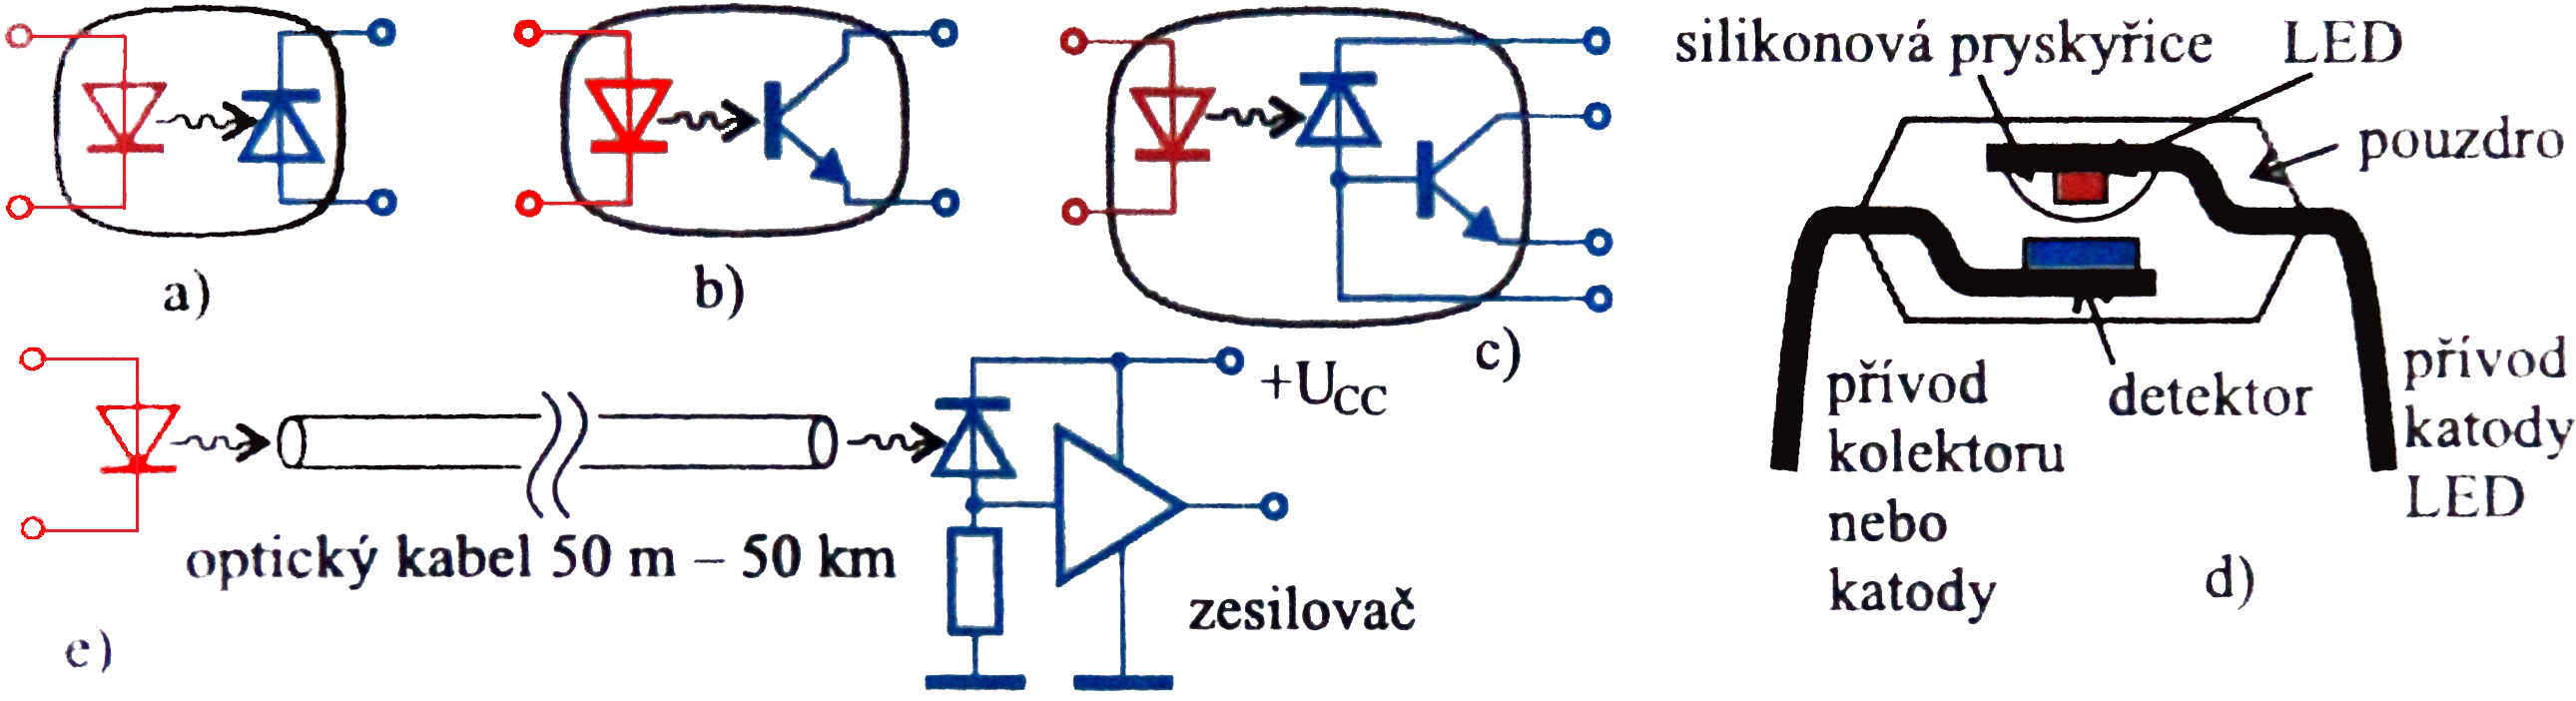
\includegraphics[width=\linewidth]{zahlava_optoel_sys.jpg}
      \caption{Optoelektronické systémy \cite[p.~179]{Zahlava2001}}
      \label{ES:fig_opto_sys}
    \end{figure}
  
    Přenos signálu mezi zdrojem a detektorem na velkou vzdálenost se provádí prostředím s malým 
    útlumem a vysokou šumovou imunitou, kterým je optické vlákno. Jedno nebo několik takových 
    vláken s povrchovou a mechanickou ochranou (z kevlaru a polyuretanu) tvoří optický kabel. 
    Vlákno se skládá z vnitřního skleněného jádra (o průměru jednotek až desítek \(\mu m\)) s 
    indexem lomu \(n\), a je pokryto tenkým skleněným pláštěm (tlustým desítky \(\mu m\)) s indexem 
    lomu \(n_2\). Jelikož \(n_1>n2\), dochází pro určité rozmezí úhlu dopadu k odrazu záření na 
    rozhraní jádro-plášť a energie záření se pak šíří převážně jádrem vlákna. Z důvodu nízkého 
    útlumu vlákna se přenos uskutečňuje v přenosových oknech \SI{850}{\nano\meter}, 
    \SI{1300}{\nano\meter} a \SI{1550}{\nano\meter}, přičemž s rostoucí hodnotou vlnové délky útlum 
    vlákna klesá, ale cena potřebných optoprvků roste.
    
    \emph{Typy optronů z hlediska aplikace:}
      \begin{itemize}
        \item optrony vyráběné pro aplikace v lineárních obvodech mají dobrou linearitu a jsou
              používány pro galvanické oddělení analogových obvodů;
        \item optrony vyráběné pro aplikace v logických obvodech jsou určeny pro přenos pouze dvou
              úrovní signálů a proto je jejich realizace podstatně snadnější než realizace
              lineárních optronů.
      \end{itemize}
  
    \subsection{Statické parametry optoelektronických vazebních systémů}
      \subsubsection{Proudový přenosový poměr CTR}\label{ES:Opto_CTR}
        Přenosovou účinnost optoelektronického vazebního systému charakterizuje \emph{proudový
        přenosový poměr CTR} (Current Transfer Ratio), který udává poměr výstupního ku vstupnímu
        proudu optronu v procentech při daném pracovním napětí (nastavení pracovního bodu), zátěži a
        teplotě. 
        \begin{equation}\label{ES:eq_CTR1}
          CTR=\frac{I_{out}}{I_{in}}\times100  \qquad\text{[\%]} 
        \end{equation}
        S fotodiodou na výstupu je \(\text{CTR}\approx0,2-0,3\,\%\) a s fototranzistorem na výstupu
        je \(\text{CTR}\approx10-100\,\%\). Tento poměr vyjádřený rovnicí \ref{ES:eq_CTR1} je
        parametr svými vlastnostmi podobný proudovému zesilovacímu činiteli bipolárního tranzistoru
        \(h_{FE}\)\footnote{nebo též \(h_{21E}\) resp. \(\beta\). Jedná se o parametr vystupující
        v hybridních rovnicích popisující chování tranzistoru v zapojení se společným emitorem.
        \(h_{21E}\) jako diferenciální proudový přenos při výstupu nakrátko} a je s ním možné
        pracovat podobným způsobem.
               
        V následujích odstavcích se budeme předpokládat optoelektronický vazební systém s
        fotodiodou na vstupu a fototranzistorem na výstupu. V tomto případě je zřejmé, že CTR udává
        v procentech poměr velikosti kolektorového proudu přijímacího tranzistoru \(I_C\) ku proudu
        vysílací diodou \(I_F\).
        \begin{equation}\label{ES:eq_CTR2}
          CTR=\frac{I_{C}}{I_{F}}\times100  \qquad\text{[\%]} 
        \end{equation}
        Poměr je udáván pro určitý proud \(I_F\) diody LED a kolektorové napětí \(U_{CE}\)
        fototranzistoru, např. \(CTR = 50\,\%\) při \(I_F = \SI{1}{\milli\ampere}\), \(U_{CE} =
        \SI{5}{\volt}\) znamená, že když fotodiodou teče proud \(\SI{1}{\milli\ampere}\), je
        výstupní kolektorový proud \(I_F = \SI{0,5}{\milli\ampere}\).
        
        \begin{itemize}
          % CTR dependency on LED input current (IF)
          \item \emph{Závislost CTR na vstupním proudu fotodiody} na obr. \ref{ES:fig_opto_CTR01},
                není dáná monotónní funkcí, tj průběhem který by jen klesal, nebo naopak jen
                narůstal, ale vykazuje extrém, při kterém je dosažený přenosový poměr maximální.
                \begin{figure}[ht!]
                  \centering
                  \subcaptionbox{Závislost CTR na vstupním proudu fotodiody \label{ES:fig_opto_CTR01}}
                      {\luafigure[0.7]{ES_opto_CTR01.jpg}}   \newline
                  \subcaptionbox{Závislost CTR na teplotě \label{ES:fig_opto_CTR03}}
                      {\luafigure[0.7]{ES_opto_CTR03.jpg}}
                  \caption{Závislost CTR na vstupním proudu fotodiody a) a teplotě b)}
                  \label{ES:fig_opto_CTRparam}
                \end{figure}
          % CTR dependency on temperature      
          \item \emph{Závislost CTR na teplotě} na obr. \ref{ES:fig_opto_CTR02} ukazuje že
                zobrazená křivka je výsledkem kombinace dvou teplotních koeficintů. Zatímco
                světelná účinnost LED\footnote{LED luminous efficiency} vykazje záporný teplotní
                koeficient, tranzistor naproti tomu kladný teplotní koeficient.
                \ref{ES:fig_opto_CTR02}. 
                \begin{figure}[ht!]
                  \centering
                  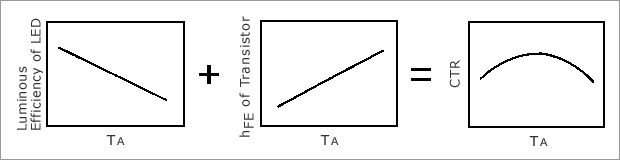
\includegraphics[width=\linewidth]{ES_opto_CTR02.jpg}
                  \caption{Závislost CTR na teplotě}
                  \label{ES:fig_opto_CTR02}
                \end{figure}
          % Change of CTR over operating time      
          \item \emph{Závislost CTR na čase} na obr. \ref{ES:fig_opto_CTR04} a obr.
                \ref{ES:fig_opto_CTR05} udává velice důležitou vlastnost, na kterou je třeba klást
                důraz v aplikacích, vyžadující dlouhou životnost produktu. Mohou to být
                například větrné elektrárny, drážní zabezpečovací zařízení atd. Největší vliv má na
                pokles CTR rychlost stárnutí fotodiody. Světelná účinnost klesá tím rychleji, čím
                větší je pracovní proud \(I_F\) viz obr. \ref{ES:fig_opto_CTR04} a čím větší je
                okolní teplota viz obr. \ref{ES:fig_opto_CTR05}. V určité formě je degradace CTR
                způsobena také stárnutím optické vazby mezi fotodiodou a fototranzistorem a změnou
                účinnosti foto-elektrické konverze a stejnosměrného zesílení
                samotného fototranzisotru tj. \(h_{FE}\).              
                % The change of the CTR over operating time is mainly caused by a drop in the
                % luminous efficiency of the LED. In general, the larger the LED input current (IF)
                % and the higher the ambient temperature, the faster the CTR decreases.
                \begin{figure}[ht!]
                  \centering
                  \subcaptionbox{vliv pracovního proudu fotodiody \(I_F\) \label{ES:fig_opto_CTR04}}
                    {\luafigure[0.9]{ES_opto_CTR04.jpg}}   \newline
                  \subcaptionbox{Závislost CTR na provozní době           \label{ES:fig_opto_CTR05}}
                    {\luafigure[0.9]{ES_opto_CTR05.jpg}}   
                  \caption{Závislost CTR na provozní době}
                  \label{ES:fig_opto_CTRtime}
                \end{figure}
        \end{itemize}      
      \       
      % -----------------Dynamické parametry optoelektronických vazebních systémů-------------------
      \subsection{Dynamické parametry optoelektronických vazebních systémů}
        Rychlost optronu je většinou limitována detektorem na výstupu. Pro rychlý přenos číslicového
        signálu se proto vyrábí optrony s fotodiodou integrovanou na jednom čipu s rychlým
        zesilovačem, jehož výstup je přímo slučitelný s číslicovými obvody. 
      %\subsection{Response time}       
        The response time of a photocoupler is similar to that of a transistor, and is expressed as
        follows. tf // RL X hFE X CCB kde \(R_L\ldots\) zatěžovací odpor, \(h_{FE}\ldots\) proudový
        zesilovací činitel tranzitoru (DC amplification) , \(C_{CB}\ldots\) kapacita mezi kolektorem
        a bází.
                      
        From this formula, tf increases as the load resistance increases as shown in Figure 6, so
        for high-speed signal transfer, the load resistance must be designed as small as possible
        within the allowable rating range.      
         \begin{figure}[ht!]
           \centering
           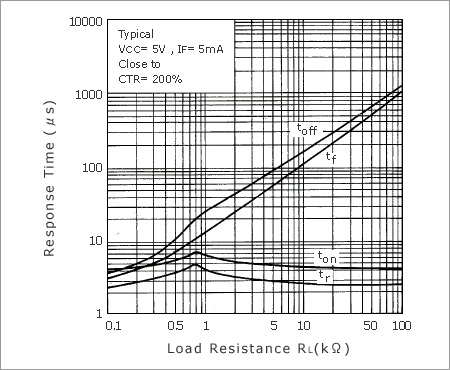
\includegraphics[width=0.8\linewidth]{ES_opto_CTR06.jpg}
           \caption{Response Time vs. RL Characteristics }
           \label{es:fig_opto_CTR06}
         \end{figure}      
      
         \begin{figure}[ht!]
           \centering
           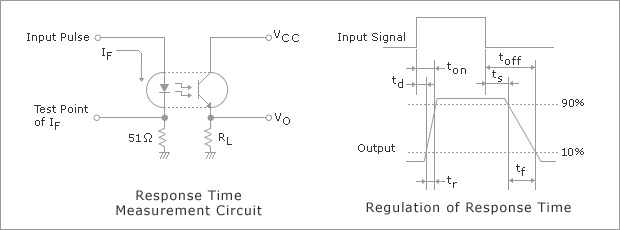
\includegraphics[width=0.9\linewidth]{ES_opto_CTR07.jpg}
           \caption{***}
           \label{es:fig_opto_CTR07}
         \end{figure}             
          However, when the load resistance is minimized, the transistor may not become completely
          ON and the output signal may be unstable unless the input current IF and output current IC
          are determined making sufficient allowance for factors such as the CTR specification
          range, the temperature characteristics, and the change over time.
                   
          Some examples of these characteristics are introduced below.      
                   
          Figure 7 shows an example of the variation in the response time according to the ambient
          temperature (TA).
         
          \begin{figure}[ht!]
            \centering
            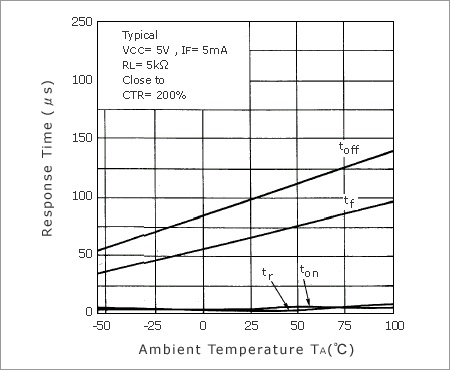
\includegraphics[width=0.8\linewidth]{ES_opto_CTR08.jpg}
            \caption{***}
            \label{es:fig_opto_CTR08}
          \end{figure}       
          Figure 8 shows an example of the variation in the response time according to the input
          current (IF).
          
          \begin{figure}[ht!]
            \centering
            \subcaptionbox{Response Time vs. IF Characteristics \label{ES:fig_opto_CTR08}}
              {\luafigure[0.9]{ES_opto_CTR09.jpg}}                   \newline
            \subcaptionbox{Response Time vs. IF Characteristics \label{ES:fig_opto_CTR09}}
              {\luafigure[0.9]{ES_opto_CTR10.jpg}}   
             \caption{Závislost CTR na provozní době}
             \label{ES:fig_opto_tfvsIF}
          \end{figure}
       
          Figure 9 shows an example of the variation in the response time according to the power
          supply current (VCC).
          
      %-------------------Izolační parametry optronu------------------------------------------------
      \subsection{Izolační parametry optronu}
        V mnoha aplikacích je na izolační bariéry, kladen jen požadavek na kvalitní galvanického
        oddělení. Galvanické oddělení je obvykle efektivním prostředkem, jak potlačit šíření rušení
        mezi systémy, neboť jednoduše dokážeme přerušit zemní a jiné impedanční smyčky v obvodě.
        Kvalita tohoto oddělení je pak závislá na velikostech parazitních kapacit mezi vstupem a
        výstupem optoelektronického prvku. V těchto obvodech je optoelektronických vazebních prvků
        použito ačkoliv, oddělované signály mají stejný vztažný potenciál (např. GND). 
        
%       Izolace, na které jsou kladeny kromě funkčích také bezpečností požadavky, kritérium
%       jmenovitého izolačního napětí rozšířeno také další požadavky, které mohou vyplývat z norem
%       zabývajících se kooridancí izolací pro daný okruh aplikací, v jejichž souladu musí 
%       být dané
%       zařízení konstruované.  Účelem těchto norem je stanovit povrhové a vzdušné vzdálenosti pro
%       daný typ pracovní prostředí a druh konstručkního materiálu izolační bariéry.  a  tvořena
%       \emph{External creepage} je definována jako nejmenší vzdálenost vedenou přes izolační
%       bariéru po povrchu pouzda mezi vodivými prvky (vývody) optronu. \emph{external clearance}
%       je chápána jako nejmenší vzdušná vzdálenost vývodů.
        \begin{figure}[hb!]
          \centering
          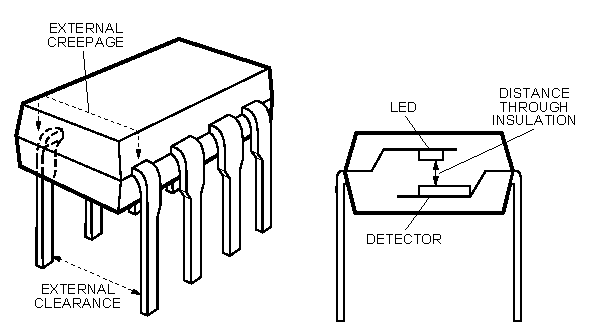
\includegraphics[width=0.7\linewidth]{optocoupler_clearance.pdf}
          \caption{K pojmu external creepage a clearance}
          \label{es:fig_optocoupler_clearance}
        \end{figure}

%} % tikzset
%---------------------------------------------------------------------------------------------------
%=============== Seznam literatury ===============================================================
\printbibliography[title={Seznam literatury}, heading=bibliography]
}  % DEBUG was off
%--------------------------------------------------------------------------------------------------
%                            /$$      /$$  /$$$$$$   /$$$$$$          /$$   /$$                                   | $$$    /$$$ /$$__  $$ /$$__  $$
%                           | $$$    /$$$ /$$__  $$ /$$__  $$        | $$$ | $$                                   | $$$$  /$$$$| $$  \ $$| $$  \__/
%                           | $$$$  /$$$$| $$  \ $$| $$  \__/        | $$$$| $$                                   | $$ $$/$$ $$| $$$$$$$$| $$ /$$$$
%                           | $$ $$/$$ $$| $$$$$$$$| $$ /$$$$ /$$$$$$| $$ $$ $$                                   /$$      /$$  /$$$$$$   /$$$$$$ 
%                           | $$  $$$| $$| $$__  $$| $$|_  $$|______/| $$  $$$$                                   | $$  $$$| $$| $$__  $$| $$|_  $$
%                           | $$\  $ | $$| $$  | $$| $$  \ $$        | $$\  $$$                                   | $$\  $ | $$| $$  | $$| $$  \ $$
%                           | $$ \/  | $$| $$  | $$|  $$$$$$/        | $$ \  $$                                   | $$ \/  | $$| $$  | $$|  $$$$$$/
%                           |__/     |__/|__/  |__/ \______/         |__/  \__/                                   |__/     |__/|__/  |__/ \______/                    
%--------------------------------------------------------------------------------------------------
\ifthenelse{ \equal{\DebugMode}{true} }{% Debug mode ON
  % !TeX program = lualatex
% !TeX root = luaking.tex
% !TeX encoding = UTF-8
% !TeX spellcheck = cs_CZ
%---------------------------------------------------------------------------------------------------
% file spojity_model_elmag_p.tex
\graphicspath{{../src/TEO/img/}}
%==============================Kapitola: Spojité matematické modely jednotlivých polí ==============
\setchaptertoc
\chapter{Spojité matematické modely polí}

  \section{Elektromagnetické pole}
    \subsection{Veličiny elektromagnetického pole a jejich jednotky}
      \fbox{Elektrický náboj} je \emph{skalární veličinou}. Jednotkou je \emph{coulomb [C]}. Má
         kvantový charakter (tj. je roven celistvému násobku elementárního náboje $e =
         1,602\cdot10^{-19}C$), avšak v technických aplikacích k tomu nepřihlížíme. Náboj $Q$
         může být rozložen:
         \begin{itemize}[noitemsep]
            \item \emph{prostorově} v objemu $V$ s objemovou hustotou
               \begin{equation}\label{TEMP:eq_q_varrho}
                  \varrho = \frac{dQ}{dV} \quad [C\cdot m^{-3}]
               \end{equation}               
            \item \emph{plošně} na ploše $S$, s plošnou hustotou
               \begin{equation}\label{TEMP:eq_q_sigma}
                  \sigma = \frac{dQ}{dS} \quad [C\cdot m^{-2}]
               \end{equation}                 
            \item \emph{lineárně} na křivce $l$, s lineární hustotou
               \begin{equation}\label{TEMP:eq_q_tau}
                  \tau = \frac{dQ}{dl} \quad [C\cdot m^{-1}]
               \end{equation}                 
         \end{itemize}
         Rozlišujeme:
           \begin{itemize}[noitemsep]
             \item \textbf{volné náboje}: mohou se přemisťovat v makroskopických
             vzdálenostech,
             \item \textbf{vázané náboje}: mohou se přemisťovat jen v
             mikroskopických vzdálenostech.
           \end{itemize}
         Volnými náboji jsou volné elektrony v kovech nebo ionty v elektrolytech (jsou odpoutány od
         atomů, resp. molekul a volně se mezi nimi pohybují); vázané náboje vznikají polarizací
         dielektrika.
         
      \vspace{1em}
      \fbox{Elektrický proud}\label{TEMP:kap_el_proud_velicina} je znám z každodenního života,
        přesto je velmi důležité umět tento pojem vnímat jak pro označení „jevu“ (kap.
        \ref{TEMP:kap_elproud_jev}), tak jako fyzikální veličinu, která tento jev kvantitativně
        popisuje (kap. \ref{TEMP:kap_el_proud_velicina} ). Elektrický proud je \emph{skalární
        fyzikální veličina} tzn. $I$ resp. $i$, jejíž jednotkou je základní jednotka soustavy SI:
        \emph{ampér} - [A]. V této soustavě jednotek je ampér definován na základě silových
        účinků mezi dvěma vodiči, kterými prochází elektrický proud. Tato síla je magnetického
        původu, avšak magnetické pole vzniká jako důsledek pohybu elektrického náboje. Je tvořen
        uspořádaným pohybem elektrických nábojů.
        
        Připojíme-li vodič ke zdroji elektrického napětí, elektrické pole uvnitř působí elektrickou
        silou na vodivostní elektrony, vyvolává jejich pohyb a tím vytváří elektrický proud, který
        je po krátké době \emph{stacionární} (ustálený, nezávislý na čase). Jestliže vodičem projde
        náboj $\Delta Q$ resp. $dQ$ za časový interval $\Delta t$ resp. $dt$, lze definovat
        \emph{průměrný} resp. \emph{okamžitý} proud ve vodiči:
        \begin{itemize}[noitemsep]
          \item \textbf{průměrný} elektrický proud: $$I_{AV} = \frac{\Delta Q}{\Delta t}
                \quad[A],$$
          \item \textbf{okamžitý} elektrický proud (který je limitním případem proudu průměrného,
                studujeme-li množství náboje, které projde průřezem vodiče za infinitezimální
                (nekonečně krátký) časový interval): $$i = \lim_{\Delta t \rightarrow 0}\frac{\Delta
                Q}{\Delta t} = \frac{dQ}{dt} \quad[A].$$ V ustáleném stavu protéká všemi průřezy
                vodiče stejně velký proud,
          \item speciálně pohybuje-li se náboj vodičem rovnoměrně, nazýváme proud
                \textbf{stejno\-směr\-ným}, $I(t) = \text{konst}$, a platí $$ I_{DC} =
                \frac{Q}{t}\quad[A] $$
        \end{itemize}        

        Elektrický proud jako \emph{jev} charakterizuje jednu z forem fyzikálního pohybu, kterou je
        \textbf{uspořádaný pohyb elektricky nabitých částic} v látce. Přestože jakýkoliv elektrický
        proud je vždy tvořen pohybujícími se náboji, nemusí všechny pohybující se náboje vytvářet
        elektrický proud. Ve vodiči dochází ke vzniku trvalého elektrického proudu za těchto
        podmínek:
          \begin{itemize}[noitemsep]
            \item vodič se musí nacházet v trvalém elektrickém poli, což je realizováno pomocí tzv.
                  \emph{zdroje} (generátoru) elektrického napětí,
            \item ve vodiči musí být přítomny volné nosiče elektrického náboje.
          \end{itemize}
        
        Podle charakteru vnějšího elektrického pole lze rozlišit tři základní druhy proudů:
          \begin{description}[noitemsep]
            \item\textbf{stejnosměrný} proud vzniká tehdy, jestliže má intenzita elektrického pole
                   konstantní orientaci,
            \item\textbf{střídavý} proud ve vodiči vytváří vnější elektrické pole, jehož intenzita
                  periodicky mění svou orientaci na opačnou,
            \item\textbf{stacionární} stejnosměrný proud vzniká ve vodiči, je-li intenzita
                  elektrického pole konstantní co do velikosti, směru i orientace.
          \end{description}  

       Nabité částice představující volný náboj ve vodičích jsou v neustálém chaotickém tepelném
       pohybu (viz molekulová fyzika a termodynamika). Jedná se o \emph{mikroskopický pohyb}, který
       nemá za následek makroskopicky pozorovatelné přemístění náboje. Pokud ve vodiči vytvoříme
       elektrické pole, tepelný pohyb nabitých částic neustane, ale k náhodné složce rychlosti
       přibude ještě složka rychlosti ve směru vloženého pole.
       
       Při studiu elektrického proudu v kovových vodičích se zabýváme ustálenými proudy
       vodivostních elektronů, které v kovu vytváří tzv. \emph{elektronový plyn}. Tyto vodivostní
       elektrony jsou téměř volné a pohybují se v poli kladných iontů uspořádaných v krystalové
       mřížce.
        
       Experimentálně lze elektromagnetické pole prokázat silovým působením na elektricky nabité
       částice (kapitola \ref{fyz:IIchapI}). Celkovou sílu $\vec{F}$ lze rozložit na elektrickou 
       sílu $\vec{F}_e$, nezávislou na tom, zda je nabitá částice v klidu nebo v pohybu vůči 
       vztažné soustavě a na magnetickou sílu $\vec{F}_m$, působící jen na pohybující se částice. 
       Elektromagnetické pole má tedy dvě složky: \textbf{elektrické pole}, působící na náboj silou 
       $\vec{F}_e$ a \textbf{magnetické pole}, působící na pohybující se náboj silou $\vec{F}_m$  
       \cite[s.~13]{Mayer2001}. 
      
      \vspace{1em}
      \fbox{Intenzita elektrického pole $\vec{E}$} je vektorovou veličinou charakterizující
        \emph{elektrické pole}.
        Je definována jako 
        \emph{síla působící na nepohybující se jednotkový bodový náboj}:
        \begin{equation}\label{TEMP:eq_E}
          \vec{E} = \frac{\vec{F}_e}{Q} \quad\left[\frac{V}{m}\right]  
        \end{equation}        
        kde $\vec{F}_e$ je elektrická síla působící na náboj $Q$.
      
      \vspace{1em}
      \fbox{Magnetická indukce $\vec{B}$} je vektorovou veličinou charakterizující \emph{magnetické
        pole}. Je definovována vztahem
        \begin{equation}\label{TEMP:eq_B}
          \vec{F}_m = Q(\vec{v}\times\vec{B}) \quad[T]  
        \end{equation}        
        kde $\vec{F}_m$ je magnetická síla působící na náboj $Q$ pohybující se rychlostí $\vec{v}$.
        Jednotkou je \emph{tesla} $[T]$.
    
        Síla, jež působí elektromagnetické pole na pohybující se náboj se nazývá \textbf{Lorentzova
        síla}
        \begin{equation}\label{TEMP:eq_Lorentz}
          \vec{F} = \vec{F}_e + \vec{F}_m =Q(\vec{E} + \vec{v}\times\vec{B}) \quad[N]  
        \end{equation}        

    \subsection{Maxwellovy rovnice}
      Makroskopická teorie elektromagnetického pole v klasickém pojetí vychází ze základních zákonů
      vyjádřených \emph{Maxwellovými rovnicemi (MR)}. Lze je zapsat buď v \textbf{integrálním} (viz 
      kap. \ref{fyz:IIchapIII}), nebo \textbf{diferenciálním tvaru} (viz kap. \ref{fyz:IIchapII}). 
      V integrálním tvaru popisují elektromagnetické pole v jisté prostorové oblasti $\Omega$, 
      kdežto v diferenciálním tvaru ve vnitřním bodě této oblasti. Soustavu vlastních MR 
      představují první čtyři páry rovnic; často se k nim připojuje jako další základní rovnice 
      elektromagnetického pole rovnice kontinuity pro vodivý proud. Její integrální a diferenciální 
      tvar reprezentují poslední dvě rovnice.
      \begin{subequations}
        \begin{alignat}{3}
          \oint_{\mathcal{C}}\vec{H} \dd{\vec{l}}, &= I+\der{\Psi}{t}
                                       \quad &&\rot{H}&&=\vec{J}+\pder{\vec{D}}{t}             \\
          \oint_{\mathcal{C}}\vec{E} \dd{\vec{l}}, &= -\der{\Phi}{t}
                                       \quad &&\rot{E}&&=-\pder{\vec{B}}{t}                    \\
           \int_{\mathcal{S}}\vec{D} \dd{\vec{S}}, &= Q \quad\quad\;   
                                       \quad &&\diver{D} &&=\rho_V                             \\
           \int_{\mathcal{S}}\vec{B} \dd{\vec{S}}, &= 0 \quad
                                       \quad &&\diver{B}&& =0                                  \\
           \int_{\mathcal{S}}\vec{J} \dd{\vec{S}}, &= -\der{Q}{t} 
                                       \quad &&\diver{J}&&=-\der{\rho_V}{t}
        \end{alignat}
      \end{subequations}

      Předpokládá se, že \emph{všechny křivky a plochy v integrálním tvaru MR jsou po částech
      hladké a všechny integrované veličiny jsou po částech spojité funkce}. Pak je zaručena
      existence integrálů v těchto rovnicích. V diferenciálním tvaru MR se předpokládají pouze
      \textbf{regulární body} oblastí, což jsou body, v nichž jsou veličiny $\vec{E}$, $\vec{D}$,
      $\vec{B}$ a $\vec{H}$ \emph{spojité a spojitě diferencovatelné funkce}; nejsou jimi tedy např.
      body rozhraní dvou různých prostředí, v elektrickém poli body v nichž jsou umístěny diskrétní
      náboje, v magnetickém poli body proudových vláken atd.

      % --------example: Energie v Kondenzátoru ------------------------
      % \label{TEO:exam019}
      % !TeX spellcheck = cs_CZ
\begin{mdframed}[style=mdexam]
  \begin{example}\label{teo:exam019}
    Mějme nabitý deskový kondenzátor \(C\) (obr. \ref{teo:fig019a}). Zvětšíme jeho kapacitu,
    například tím, že zvětšíme plochu jeho elektrod, nebo připojíme paralelně druhý stejné
    velikosti, viz obr. \ref{teo:fig019b}. Otázka zní, jak velká energie bude uložena v
    elektrostatickém poli obou kondeznátorů? Bude energie po rozdělení náboje mezi oba kondenzátory
    rovna původní energii nabitého kondenzátoru? Pokud ne, vysvětlete kam se část energie
    transformovala. 
    
    {\centering
      \captionsetup{type=figure}
      \subcaptionbox{\label{teo:fig019a}}{\luafigure[0.15]{teo_fig019a.png}}           
      \hspace{1em}
      \subcaptionbox{\label{teo:fig019b}}{\luafigure[0.35]{teo_fig019b.png}}
      \hspace{1em}
      \subcaptionbox{\label{teo:fig020}}{\luafigure[0.30]{teo_fig020.png}}
      \captionof{figure}{K příkladu \ref{teo:exam019}: a) Nabitý kondenzátor s rovnoběžnými
      rovinnými elektrodami; b) Rozložení náboje na obou kondenzátorech stejné velikosti; c)
      Rezistor \(R\) představuje ztráty, které nebyly v obvodu na obrázku \ref{teo:fig019b}
      předpokládány}
      \label{teo:fig019}
    \par}
    
    Je-li dielektrikum kondenzátoru lineární, pak pro energii elektrického pole akumulované v
    nabitém kondenzátoru platí. Podrobněji například v kapitole \ref{fyz:IIchapVsecXIX}.
    \begin{equation}
      W = \frac{1}{2}CU^2 \;\text{nebo}\; W = \frac{1}{2}\frac{Q^2}{C} \;\text{kde}\; 
      C = \frac{Q}{U}
    \end{equation}
    Předpokládejme ustálený stav po připojení druhého kondenzátoru, jak je znázorněno na obr.
    \ref{teo:fig019b}. V obvodu nepředpokládáme přítomnost odporu, který by způsobil ztrátu energie,
    vyzářené v podobě tepla. Kapacita je dvojnásobná a náboj zůstal stejný. Na každém kondenzátoru
    tedy očekáváme polovinu původního náboje. Sečteme-li energii uloženou v elektrických polích obou
    kondenzátorů dostaneme
    \begin{align*}
      W^* &= \frac{1}{2}\frac{(\frac{1}{2}Q)^2}{C} + \frac{1}{2}\frac{(\frac{1}{2}Q)^2}{C}   \\
          &= \frac{(\frac{1}{2}Q)^2}{C} =\frac{1}{4}\frac{Q^2}{C}                 
           \xrightarrow[C\rightarrow2C]{}
            \frac{1}{2}\frac{Q^2}{(2C)} = \frac{1}{2}W 
    \end{align*}
    Kupodivu, polovina energie prostě chybí a jelikož platí zákon zachování energie\footnote{viz
    partie Fyzika \ref{vol02:part:FYZI}, kapitola \ref{vol02:fyz:IchapIV})}, nezbývá nic jiného než
    uznat, že elektrický obvod dle \ref{teo:fig019b}, nemodeluje fyzikální problém dost věrně. Tím
    jsme dospěli k závěru, že je nutné do obvodu dodat rezistor, tak jak je znázorněno na obrázku
    \ref{teo:fig020}.
    
    Abychom mohli určit tepelné ztráty na rezistoru dané integrálem \(\int_{0}^{\infty}
    Ri^2(t)\dd{t}\), nejdříve sestavíme jednoduchou diferenciální rovnici prvního řádu aplikací II.
    Kirchhoffova zákona, ze které odvodíme vzorec pro časovou závislost proudu \(i(t)\). 
    \begin{align*}
      \frac{Q_0 - Q}{C} - Ri(t) - \frac{Q}{C}           &= 0 \quad/\der{ }{t}             \\
      -\frac{i(t)}{C} - R\der{i(t)}{t} - \frac{i(t)}{C} &= 0                              \\
                                          \der{i(t)}{t} &= - \frac{2}{RC}i(t) \quad/\int  \\
                                                   i(t) &= I_0e^{-\frac{2}{RC}t}
    \end{align*}
    Nyní můžeme stanovit energii disipované na rezitoru \(R\)
    \begin{align*}
      W   &= \int_{0}^{\infty}Ri^2(t)\dd{t} = RI_0^2\int_{0}^{\infty}e^{-\frac{4}{RC}t}\dd{t}   \\
      \shortintertext{Do integrované funkce dosadíme novou proměnnou \(u = \frac{4}{RC}t\), \(\dd{u} 
                      = \frac{4}{RC}\dd{t}\), \(\dd{t} = \frac{RC}{4}\dd{u}\)}
          &= RI_0^2\int_{0}^{\infty}e^{-u}\frac{RC}{4}\dd{u} 
          = R^2I_0^2\frac{C}{4}\underbrace{\int_{0}^{\infty}e^{-u}\dd{u}}_1 
      \end{align*}
    Jelikož platí \(I_0 = \frac{U}{R}=\frac{Q}{CR}\) dostaneme po dosazení
    \(\cancel{R^2}\frac{Q^2}{C^2\cancel{R^2}}\frac{C}{4} = \frac{Q^2}{4C}= \frac{1}{2}W\). Nyní je
    vše v pořádku. Druhá polovina energie je disipována na rezistoru a navíc z výsledku vyplývá, že
    vůbec nezávisí na \(R\)!
  \end{example}
\end{mdframed}  
      %-----------------------------------------------------------------
      
  % --------------- Stacionární magnetické pole-----------------------------------------------------
  \section{Stacionární proudové pole}
    V elektrostatice (tj. elektrickém poli nepohybujících se nábojů) neexistuje trvalý elektrický
    proud. Zdroje napětí (galvanické články, termočlánky, dynama aj.) mají tu vlastnost, že na
    jejich záporné svorce je trvale nadbytek elektronů, a na jejich kladné svorce jejich nedostatek.
    Těmito zdroji můžeme ve vodiči trvale udržovat elektrické pole a tedy i tok nosičů elektřiny.
    Jestliže se \emph{náboje pohybují konstantní rychlostí, hovoříme o stacionárním elektrickém
    proudu}. Základní rovnice elektrostatické pole jsou:

    \begin{table}[ht!]
      \centering
      \begin{tabular}{m{0.1\linewidth}|m{0.29\linewidth}|m{0.34\linewidth}|}
        \cline{2-3}
        \multicolumn{1}{l|}{} 
          & \textbf{integrální tvar} & \textbf{diferenciální tvar}                              \\
        \hline        
        \multicolumn{1}{|m{0.19\linewidth}|}{2. MR}         
          & \(\bigointsss\vec{E}\cdot \dd{\vec{l}} = 0\) & \(\rot{E} = 0\)                      \\ 
        \cline{1-3}       
        \hline        
        \multicolumn{1}{|m{0.19\linewidth}|}{Zákon kontinuity}        
          & \(\bigointsss\vec{J}\cdot \dd{\vec{S}}=0\) & \(\diver{J}=0\)                        \\
        \cline{1-3}       
        \multicolumn{1}{|m{0.19\linewidth}|}{Ohmův zákon}       
          & \(I=GU=\dfrac{U}{R}\) & \(\vec{J} = \gamma\vec{E} = \dfrac{1}{\rho}\vec{E}\)        \\
        \cline{1-3}
      \end{tabular}
      \caption{Základní rovnice stacionárního proudového pole}
    \end{table}
    
    \subsection{Elektrický proud v kovových vodičích}\label{TEMP:kap_elproud_jev}
      V předchozí kapitole \ref{TEMP:kap_el_proud_velicina} bylo o elektrickém proudu pojednáváno
      jako o skalární fyzikální veličině. V této kapitole nás bude zajímat makroskopický pohled na
      „jev“ známý jako \emph{elektrický proud}.
      
      Zopakujme, že elektrickým proudem je míněn uspořádaný pohyb elektrických ná\-bo\-jů, a aby se
      tyto náboje mohly pohybovat, musí být volné - jsou přítomny v látkách, které nazýváme
      \textbf{vodiče}. Vodiče mohou mít nositele náboje jednoho znaménka (elektrony v kovech,
      uhlíku a v polovodičových) anebo obojích znamének (kladné a záporné ionty v elektrolytech,
      ionty a elektrony v ionizovaných plynech). Volné nositele náboje (elektrony, ionty) lze
      rovněž oddělit od těchto látek (vodičů) a vytvořit elektrický proud ve vakuu nebo ve
      zředěných plynech.
      
      Z vodičů mají největší význam \textbf{kovy}, které jsou polykrystalickými látkami s kovovou
      vazbou. Každý mikroskopický monokrystal kovu má pevnou krystalovou mříž sestavenou z kladných
      iontů, mezi nimiž se přetržitě pohybují \emph{volné elektrony} rychlost\-mi, jejichž velikost
      je statisticky proměnná (co do velikosti i směru). Střední hodnota rychlosti (jako vektoru)
      všech elektronů je nulová. Střední hodnota rychlosti určitého elektronu je závislá na teplotě
      vodiče. Elektrony konají tzv. \emph{termický pohyb}. Rychlosti neuspořádaných termických
      pohybů dosahují jen o několik řádů větších hodnot, než kmity iontů v krystalech mřížky.

      \luagraphic[0.8]{vd_e_drift.pdf}{Pohyb elektronu ve vodiči. Fyzikálně je $v_d$ průměrná
        rychlost nosičů náboje uvnitř vodiče, který je vložen do vnějšího elektrického pole. Ve
        skutečnosti se ale elektron ve vodiči nepohybuje po přímce, jeho pohyb je
        chaotický.}{TEMP:fig_vd_e_drift}

      
      Připojíme-li vodič k vnějšímu zdroji elektrického pole (např. ke galvanickému článku), začne
      statisticky převládat uspořádaný pohyb nosičů kladného (záporného) náboje ve směru (proti
      směru) vnějšího pole nad termickým pohybem, což v makroskopickém měřít\-ku pozorujeme jako
      \textbf{makroskopický elektrický proud}. Jsou-li ve vodiči přítomny nosiče náboje obou
      polarit, dojde k pohybu ve vzájemně opačných směrech, přičemž směr toku nosičů kladného
      náboje se historicky ztotožňuje se směrem toku elektrického proudu. U kovových vodičů je tedy
      směr proudu právě opačný, než směr toku elektronů, jenž tento elektrický proud tvoří.
      
      Velikost (intenzitu) proudu posuzujeme podle velikosti náboje obojí polarity, který projde
      určitým průřezem vodiče ve vzájemně opačných směrech za jednotku času. Projde-li průřezem
      vodiče celkově náboj $dQ$ za čas $dt$, bude tok náboje vodičem charakterizovat skalární
      veličina
        \begin{equation}\label{TEMP:eq_I_01}
          I = \frac{dQ}{dt} \quad[A],  
        \end{equation}        
      která se nazývá \emph{elektrický proud} ($1C\cdot s^{-1} = 1A $ čteno \emph{ampér}). Tato
      jednotka patří mezi základní jednotky \texttt{SI} soustavy.
      
      Pro \emph{stacionární} (tj. časově neproměnný - ustálený) proud můžeme obecný výraz
      \ref{TEMP:eq_I_01} nahradit rovnicí
        \begin{equation}\label{TEMP:eq_I_02}
          I = \frac{Q}{t}.  
        \end{equation}       
      Jedná-li se o rovnoměrný pohyb bodového náboje $Q$ po kružnici s periodou $T$, resp. s
      úhlovou rychlostí $\omega$, můžeme vzniklý ustálený proud vyjádřit rovnicí 
        \begin{equation}\label{TEMP:eq_I_03}
          I = \frac{Q}{T} = \frac{\omega Q}{2\pi}.  
        \end{equation}
      
      Bude-li se element náboje $dQ$ pohybovat v lineárním útvaru rychlostí $v = \der{l}{t}$, bude 
      po dosazení do rov.\ref{TEMP:eq_I_01} reprezentovat elektrický proud 
        \begin{equation}\label{TEMP:eq_I_04}
          I = \frac{dQ}{dt} = \frac{dQ}{dl}v = \tau v, 
        \end{equation}      
      kde $\tau$ je \emph{délková hustota} náboje a $v$ je velikost \emph{okamžité rychlosti}
      náboje v uvažovaném místě lineárního útvaru. 

      \luagraphic[0.8]{teo_fig063.pdf}{Směr elektrického proudu byl implicitně stanoven jako směr
        pohybu kladných nábojů. Nositeli elektrického náboje uvnitř vodičů jsou ovšem záporně nabité
        volné elektrony, které se tedy dle  konvence pohybují proti směru elektrického proudu.
        Elektrický proud může protékat pevnými látkami (kovy, polovodiči), kapalinami (elektrolyty)
        a ionizovanými plyny. Látky, které nevedou elektrický proud, nazýváme nevodiči,
        izolanty}{teo:fig063}
      
      Elektrický proud je veličina, která obecně popisuje prostorový jev. Omezíme se nyní na běžný
      případ vodiče, jako je na obr. \ref{teo:fig063}, který má volné náboje jen jedné polarity (u
      kovových vodičů jde o elektrony) a označme $\rho_0$ prostorovou hustotu volného náboje a $v_d$
      velikost usměrněné rychlosti jejich nositelů (elektronů). Pak za čas $dt$ projde průřezem o
      obsahu $S_0$ ($S_0\bot v_d$) náboj $dQ = \rho_0 S_0 v_d dt$. Elektrický proud vyjádřený rov.
      \ref{TEMP:eq_I_01} můžeme přepsat do tvaru
        \begin{equation}\label{TEMP:eq_I_05}
          I = \rho_0 S_0 v_d = - e n_0 S_0 v_d, 
        \end{equation}         
      kde $\displaystyle{n_0 = \frac{\rho_0}{-e}}$ je počet nositelů volného náboje (tj. v našem
      případě elektronů, z nichž každý nese náboj $-e$ v jednotkovém objemu vodiče, přičemž pro
      elektrony zřejmě je $\rho_0<0$.

      Rovinnou plochou $S$ průřezu můžeme zavést jako vektor $\vec{S}$, který má směr daný normálou
      k ploše a pravidlem pravé ruky (ukazují-li prsty pravé ruky směr oběhu po hraniční křivce
      plochy, ukáže palec směr plochy jako vektoru $\vec{S}$). Protože driftová rychlost $v_d$ je
      také vektor, nebudeme obecně uvažovat vektory $\vec{S}, \vec{v_d}$ o stejném směru a rovnici
      \ref{TEMP:eq_I_05} přepíšeme do obecnějšího tvaru
      
      \begin{equation}\label{TEMP:eq_I_06}
        I = \rho_0 \vec{S_0}\cdot\vec{v}_d = jS\cos\alpha = jS_0, 
      \end{equation}      
      kde $S_0 = S$ pro $\alpha = 0$ (viz obr. \ref{teo:fig064}) a  
      \begin{equation}\label{TEMP:eq_I_07}
        \vec{j} = \rho_0\vec{v_d}, 
      \end{equation}        
      je proudová hustota. Je to vektor o velikosti
      \begin{equation}\label{TEMP:eq_I_08}
        j = \frac{I}{S\cos\alpha} = \frac{I}{S_0}  \quad A\cdot m^{-2}, 
      \end{equation}   
      obecněji
      \begin{equation}\label{TEMP:eq_I_09}
        j = \frac{dI}{dS}, 
      \end{equation}

      \luagraphic[0.6]{teo_fig064.pdf}{Rovinná plocha \(S = S_0\cos\alpha\).}{teo:fig064}
      o směru vektoru driftové rychlosti nositelů kladného náboje. Pro případ nositelů volného
      náboje - elektronů má proudová hustota opačný směr než driftová rychlost $v_d$ (obr.
      \ref{teo:fig064}).
      
      Velikost vektoru $\vec{j}$ má význam plošné hustoty elektrického proudu v uvažovaném místě
      průřezu. Jednotkou je $A\cdot m^{-2}$.
      
      Nebude-li proudová hustota na uvažovaném průřezu konstantní, bude celkový elektrický proud
      procházející průřezem o obsahu $S$ dán integrálem 
        \begin{equation}\label{TEMP:eq_I_10}
          I = \int_S \vec{j}\dd{\vec{S}}. 
        \end{equation} 

      % --------example: Driftová rychlost elektroknů ve vodiči --------
      % \label{TEO:exam008}
      % !TeX spellcheck = cs_CZ
%---------- Driftová rychlost elektroknů ve vodiči: 
\begin{mdframed}[style=mdexam]
\begin{example}\label{TEO:exam008} \emph{Driftová rychlost elektronů ve vodiči:} Vodičem z 
jednomocné mědi o
  průřezu $S_0 = \SI{1}{\mm^2}$ prochází elektrický proud $I = \SI{5}{\A}$. Vypočtěte:
  \begin{itemize}[noitemsep, leftmargin=2em]
    \item počet volných elektronů v jednotkovém objemu \ce{Cu},
    \item úhrnný náboj volných elektronů v jednotkovém objemu,
    \item driftovou rychlost volných elektronů při proudu \(I\).
  \end{itemize}
  Měď má poměrnou atomovou hmotnost $A_r = 63,54$ a hustotu\footnote{Pro hustotu budeme používat 
  alternativní značku $s$, s ohledem na kolizi značky $\rho$, jež označuje hustotu náboje.} $s = 
  \SI{8.93e3}{\kg.\m^{-3}}$.\newline  
  \textbf{Řešení:}
  \begin{itemize}[leftmargin=2em]
    \item Jeden mol mědi o molové hmotnosti $M = \SI{0.06354}{\kg\per\mol}$ a o molovém
          objemu 
          \begin{align*}
            V_m &= \frac{M}{s} 
                 = \frac{\SI{63.54e-3}{\kg.\mol^{-1}}}{\SI{8.93e3}{\kg.\m^{-3}}}      \\
                &= \SI{7.12e-6}{\m^3.\mol^{-1}}
          \end{align*}
          obsahuje $N_A = 6,0221\cdot10^{23}$ jednoatomových molekul \emph{Cu} na jeden mol,
          z nichž každý má volný jeden (valenční) elektron. Tedy počet volných elektronů v
          jednotkovém objemu je 
          \begin{align*}
            n_0 &= \frac{N_A}{V_m} = \frac{sN_A}{M}                                           
                 = \frac{\SI{6.0221e23}{\mol^{-1}}}{\SI{7.12e-6}{\m^{3}.\mol^{-1}}}    \\
                &= \SI{8.46e28}{\per\cubic\m}.
          \end{align*}  
    \item Úhrnný náboj volných elektronů v jednotkovém objemu mědi je 
          \begin{equation}
            Q_v = -e\cdot n_0 = \SI{-1.36e10}{\coulomb.m^{-3}}.
          \end{equation}
    \item Velikost driftové rychlosti určíme ze vztahu $I = -en_0v_dS_0 = - Q_v v_d S_0$ tj.
    \begin{align*}
      v_d &= \left\lvert\frac{I}{Q_v\cdot S_0}\right\rvert                       
           = \frac{\SI{5}{\coulomb\per\s}}{\SI{1.36e10}{\coulomb.m^{-3}}\cdot\SI{1e-6}{\m^2}}   \\
          &= \SI{3676e-4}{\m\per\s} = \SI{0.3676}{\mm\per\s}.  
    \end{align*}
  \end{itemize}
  Z provedených výpočtů si můžeme udělat názor o mikroskopických poměrech v kovových vodičích: počet
  volných nositelů náboje - elektronů a jejich úhrný náboj v jednotkovém objemu je značný a proto
  driftová rychlost elektronů potřebná k vyvolání proudu běžné velikosti v drátových vodičích je
  nesmírně malá (doslova hlemýždí).
\end{example}  
\end{mdframed}
  
      %-----------------------------------------------------------------

      % --------example: Velikost náboje v minci -----------------------
      % \label{TEO:exam009}
      % !TeX spellcheck = cs_CZ
%---------- Velikost náboje v minvi:
\begin{example}
  Elektricky neutrální měděná mince o hmotnosti \(m = \SI{3.11}{\g}\) obsahuje stejné množství 
  kladného a záporného náboje. Jaké je velikost kladného (nebo záporného) náboje obsaženého v 
  minci?\newline  
  \textbf{Řešení:}\newline
  Neutrální atom má záporný náboj \(Z\cdot e\), představovaný jeho elektrony a kladný náboj o 
  stejné velikosti představovaný protony v jádře. Pro měď je atomové číslo \(Z\) rovno \num{29}, 
  tj. atom mědi má \num{29} protonů, a je-li elektricky neutrální, také \num{29} elektronů.
  
  Náboj o velikosti \(Q_v\), který hledáme je roven \(N\cdot Z\cdot e\), kde \(N\) je počet atomů 
  obsažených v  jednom molu (Avogadrova konstanta: \(N_A = \SI{6.0221e23}{\per\mole}\)). Počet 
  molů mědi v minci \(\frac{m}{M}\), kde \(M = \SI{63.5}{\g\per\mole}\) je molární hmotnosti mědi: 
  \begin{equation*}
    N = N_A\cdot\frac{m}{M} = \SI{6.0221e23}{\per\mole}
           \frac{\SI{3.11}{\g}}{\SI{63.5}{\g\per\mole}} 
      = \num{2.95e22}.
  \end{equation*}
 Velikost celkového kladného (záporného) náboje v minci je pak 
  \begin{equation*}
    Q_v = N\cdot Z\cdot e = \num{2.95e22}\cdot\num{29}\cdot\SI{1.602e-19}{\coulomb} 
        = \SI{137039}{\coulomb}
  \end{equation*}
  To je obrovský náboj. Pro srovnání: třeme-li ebonitovou tyč vlněnou látkou, můžeme na tyč 
  přemístit stěží náboj o velikosti \SI{1e-9}{\coulomb}.
\end{example} 
  
      %-----------------------------------------------------------------

    % ----------------Práce a výkon elektrického proudu-----------------
    \subsection{Práce a výkon elektrického proudu}
      % --------example: Ponorný vařič ---------------------------------
      % \label{TEO:exam010}
      % !TeX spellcheck = cs_CZ
%---------- Ponorný vařič:
\begin{example}
  Za jakou dobu uvede ponorný vodič o příkonu $600\ W$ do varu $1\ l$ vody o počáteční teplotě 
  $20°C$. Uvažujte měrnou tepelnou kapacitu vody $c = 4200\ J\cdot kg^{-1}\cdot K^{-1}$. Výměnu 
  tepla s okolím neuvažujte. \newline 
  \textbf{Řešení:}\newline Pro var vody bude zapotřebí tepla dle rovnice $Q  = m\cdot c\cdot(T_2 - 
  T_1)$. Potřebná elektrická práce je $Q_e = P\cdot t = U\cdot I\cdot t$ a tedy dobu ohřevu 
  stanovíme z rovnice:
  \begin{align*}
  P\cdot t &= m\cdot c\cdot(T_2 - T_1)               \nonumber  \\
  t &= \frac{m\cdot c}{P}\cdot(T_2 - T_1)     \nonumber  \\
  t &= \frac{1\cdot 4200}{600}\cdot(100 - 20) = 560\ s
  \end{align*}         
\end{example}  
      %-----------------------------------------------------------------
 
    % ----------------Ohmův zákon------------------------------------------------------------------
    \subsection{Ohmův zákon}
      Uvažujme vodič u něhož jsou volnými nositeli náboje \emph{elektrony}. Nyní v mezích klasické
      mechaniky kvantitativně popíšeme mechanismus vedení proudu, který povede k všeobecně známému
      \textbf{Ohmovu zákonu}
      
      Umístíme-li vodič do elektrického pole o intenzitě $\vec{E}$ (např. připojením ke
      galvanickému článku), působí na každý volný elektron síla $\vec{F} = -e\vec{E}$, která mu
      podle \emph{Newtonova zákona} udělí zrychlení $\vec{a} = \frac{\vec{F}}{m_e} = -
      \frac{e}{m_e}\vec{E}$ proti směru vnějšího pole. Tím získávají chaoticky se pohybující
      elektrony ještě složku rychlosti v protisměru vloženého elektrického pole $\vec{E}$ a  dojde
      tedy k usměrnění driftového pohybu volných elektronů a v souladu s kapitolou
      \ref{TEMP:kap_elproud_jev} pozorujeme, že ve vodiči vznikl makroskopický elektrický proud.
      
      Pohyb elektronu se ovšem neobejde bez srážek s ionty v krystalové mřížce. Dráhu, kterou se
      elektronu podaří urazit, nazýváme \emph{volnou dráhou} $d$. Průměrná doba mezi dvěma po sobě
      jdoucími srážkami nechť je $\tau$ za tuto dobu se bude elektron rovnoměrně urychlovat a těsně
      před následující srážkou jeho rychlost dosáhne maxima tj. $\vec{v}_{max} = \vec{a}\cdot\tau$.
      Nás ovšem zajímá průměrná rychlost (\emph{driftová rychlost}) na volné dráze průměrné
      velikosti:
      \begin{equation}\label{TEMP:eq_vd_01}
        \vec{v}_d = \frac{\vec{v}_{max}}{2} =\frac{\vec{a}_{max}\cdot\tau}{2} 
                  = -\frac{e\tau}{2m_e}\vec{E}
      \end{equation}   
      Proudová hustota \ref{TEMP:eq_I_07} bude
      \begin{equation}\label{TEMP:eq_j_02}
        \vec{j} = \rho_0\vec{v}_d= -en_0\vec{v}_d = -\frac{e^2n_0\tau}{2m_e}\vec{E}
      \end{equation}       
      Koeficient úměrnosti 
      \begin{equation}\label{TEMP:eq_g_03}
        \gamma = \frac{e^2n_0\tau}{2m_e}
      \end{equation}     
      je závislý na počtů nositelů (elektronů) $n_0$ v jednotkovém objemu a na době $\tau$, neboli
      na délce volné dráhy. Veličina $\gamma$ se nazývá \emph{měrná elektrická vodivost} neboli
      \textbf{konduktivita} látky. Protože dobu $\tau$ nelze přímo měřit, určuje se $\gamma$
      experimentálně. Přitom se zjišťuje, že pro určitou teplotu zkoumané látky je $\gamma$
      konstantní.
      
      Po zavedení pojmu měrná elektrická vodivost látky \ref{TEMP:eq_g_03}, můžeme výraz
      \ref{TEMP:eq_j_02} přepsat do výsledného tvaru
      \begin{equation}\label{TEMP:eq_j_04}
        \vec{j} = \gamma\vec{E},
      \end{equation}              
      který se v literatuře označuje jako \emph{Ohmův zákon v diferenciálním tvaru} (i když se v
      pravém slova smyslu o diferenciální tvar nejedná). Výstižnější je označení \emph{lokální tvar
      Ohmova zákona}, protože výraz \ref{TEMP:eq_j_04} se vztahuje na určité místo, resp. bod,
      vodivého prostředí. Vztah říká, že proudová hustota v určitém bodě vodivého prostředí je
      přímo úměrná intenzitě vloženého elektrického pole v tomto bodě (platí pro určitou teplotu
      prostředí).
      
      Uvažujme nyní lineární homogenní vodič délky $l$ a příčného průřezu o obsahu $S_0$, připojený
      ke zdroji o napětí $U$. Pak intenzita pole uvnitř vodiče bude mít konstantní velikost
      $E=\frac{U}{l}$. Dosadíme-li za velikost proudové hustoty $j=\frac{I}{S_0}$ do
      \ref{TEMP:eq_j_04}, dostaneme vztah
      \begin{equation}\label{TEMP:eq_j_05}
        \frac{I}{S_0} = \gamma\frac{U}{l},
      \end{equation}        
      z něhož vyplývá známý vztah
      \begin{equation}\label{TEMP:eq_j_06}
        U = \frac{l}{\gamma S_0}I = RI,
      \end{equation}              
      kde
      \begin{equation}\label{TEMP:eq_j_07}
        R = \frac{l}{\gamma S_0} = \rho\frac{l}{S_0},
      \end{equation} 
      je \textbf{elektrický odpor} uvažovaného lineárního vodiče, přičemž $\rho = \frac{1}{\gamma}$
      je \emph{měrný elektrický odpor} (\textbf{rezistivita})\footnote{Zde je další kolize značky
      $\rho$. Nyní se tomuto problému vyhneme využíváním pouze konduktivity, jenž se častěji
      používá v teorii elektromagnetického pole.}. Výraz \ref{TEMP:eq_j_07} představuje klasický
      Ohmův zákon zákon experimentálně objevený r. 1826 \emph{G. S. Ohmem}. Jednotky:
      \begin{itemize}[noitemsep]
        \item elektrický odpor: \si{\V\per\A},
        \item měrný elektrický odpor: \si{\ohm\m},
        \item měrná elektrická vodivost: \si{\per\ohm\per\m}.
      \end{itemize}

      % --------example: Zemnicí elektroda -------------------
      % \label{TEO:exam011}
      % !TeX spellcheck = cs_CZ
\begin{example}
  \textbf{Zemnicí elektroda}: Uvažujte zemnicí elektrodu ve tvaru koule o poloměru  
  $a=\SI{200}{\mm}$, uloženou do zeminy v hloubce, která je značně větší než je poloměr $a$. Pro 
  jednoduchost řešení dále předpokládejte, že přívodní drát je od zeminy izolován (obr.
  \ref{TEMP:fig_zem_elektroda}). Zemina má měrnou vodivost $\gamma=\num[exponent-product =
  \cdot]{1,8e-2}\si{\per\ohm\per\m}$. Při zkratu teče přívodním drátem proud $I=\SI{50}{\A}$.
  Vypočítejte:
  
  %----------------------------------
  % image: TEMP_zem_elektroda.tex label: \label{TEMP:fig_zem_elektroda}
  % \documentclass{article}
% \usepackage{tikz}
% \usetikzlibrary{decorations.markings}
% \usetikzlibrary{intersections}
% \usetikzlibrary{calc}

% \begin{document}
   {\centering  
    \begin{tikzpicture}[scale=0.8, every node/.style={scale=1}]
      \coordinate (pCenter) at (0,-5);
      \fill[brown!60] (-2,-0.2) rectangle (2,-7);
      \draw[color=brown, line width=5pt] (-2,-0.2) -- +(4,0); 
      \draw[->,line width=1pt] (0,1) node[left] {$I$} -- (0,-0.1);        
      \draw[line width=1pt] (0,0) -- (pCenter);
      \draw[line width=1pt,color=black, fill=white]
           (pCenter) circle[radius=0.5];
      \draw[line width=1pt, dotted]
           (pCenter) circle[radius=1];
      \foreach \angle in
          {0, 30, 60, 120, 150, 180, 210, 240, 270, 300, 330}
      {
        \draw[->, line width=0.75pt] (pCenter)++(\angle:1.2) -- +(\angle:0.3);        
      }
      \draw[<->, thick] (pCenter)++(240:1) coordinate(pR) -- (pCenter) -- +(330:0.5) coordinate(pA); 
      \node[above] at ($ (pCenter)!0.5!(pA) $) {$a$};     
      \node[above] at ($ (pCenter)!0.9!(pR) $) {$r$}; 
      \node[above] at (-1,-2) {$\gamma$};
      \node[above] at (+1.5,-4.5) {$\vec{j}$};
    \end{tikzpicture}
    \captionsetup{type=figure}
    \captionof{figure}{Zemnicí elektroda}
    \label{TEMP:fig_zem_elektroda}
  \par}
  
% \end{document}    
  %----------------------------------         
  \begin{enumerate}[label=\emph{\alph*})]
    \item Závislost potenciálu $\varphi=\varphi(r)$ elektrického pole, které se vytvoří v
          zemině při zkratu, kde $r$ je vzdálenost od středu elektrody. Potenciál normujte
          volbou $\varphi(\infty)=0$.
    \item Zemnicí odpor elektrody, který je definován vztahem $$R_z=\frac{U_z}{I_z},$$ kde
          $U_z = \varphi(a)-\varphi(b)$ je zemnicí napětí 
    \item Ztrátový výkon při zkratu.            
  \end{enumerate}
  Řešení:    
  Ekvipotenciální a proudové plochy mají zřejmě kulový tvar se středem totožným s geometrickým 
  středem elektrody. Proudová hustota na kulové ploše obecného poloměru $r$ (viz. obr. 
  \ref{TEMP:fig_zem_elektroda}) je $$\vec{j}=\frac{I}{4\pi r^2}\vec{n},$$ kde $\vec{n}$ je 
  jednotkový vektor ve směru normály. Pak v bodech na této ploše musí být elektrické pole o 
  intenzitě $\vec{E}$, kterou určíme ze vztahu
  \begin{equation*}
    \vec{j}= \gamma\vec{E}\rightarrow\vec{E}=
    \frac{\vec{j}}{\gamma}=\frac{I}{4\pi\gamma r^2}\vec{n}.
  \end{equation*}
  Závislost potenciálu $\varphi=\varphi(r)$ tohoto elektrického pole stanovíme pomocí následujícího 
  integrálu
  \begin{equation}
    \varphi = - \int\vec{E}d\vec{r}+C = -\frac{I}{4\pi\gamma}\int\frac{dr}{r^2} + C 
            =   \frac{I}{4\pi\gamma r} + C, \nonumber
  \end{equation} 
  kde integrační konstantu $C$ určíme z okrajové podmínky $\varphi(\infty)=0$, odkud $C=0$.
  Hledaná závislost potenciálu je
  \begin{equation*}
    \varphi = \frac{I}{4\pi\gamma r}, \qquad r\in\langle a, \infty). 
  \end{equation*}           
  
  Zemina, v níž je uložena elektroda, je vlastně rezistorem, jehož jeden okraj tvoří elektrodu
  a druhým okrajem je nekonečně rozlehlý vodivý prostor. Potenciální rozdíl mezi těmito okraji je
  \begin{equation*}
    U_z = \varphi(a) - \varphi(\infty)= \frac{I}{4\pi\gamma a},
  \end{equation*} 
  \begin{minipage}[t]{0.5\textwidth}% first column            
    odkud zemnicí odpor 
    \begin{equation*}
      R_z = \frac{U_z}{I} = \frac{1}{4\pi\gamma a} = \SI{22,1}{\ohm}
    \end{equation*}
  \end{minipage}
  \begin{minipage}[t]{0.5\textwidth}% second column    
    a ztrátový výkon 
    \begin{equation*}
      P_z = R_z\cdot I^2 = \SI{55,3}{\kilo\watt}. 
    \end{equation*}
  \end{minipage}
\end{example}


  
      %-------------------------------------------------------

    % ------------------- Elektromotorické napětí -------------------------------------------------
    \subsection{Elektromotorické napětí}
      Uzavřený proudový okruh $C$, nechť je v dynamické rovnováze - prochází jím ustálený
      elektrický proud. Uvažujme pro jednoduchost představy kladný náboj - ten se musí pohybovat ve
      směru klesajícího potenciálu (záporný náboj ve směru stoupajícího potenciálu). Je-li okruh
      uzavřený, musí kladné náboje opět vystoupit na místo s vyšším potenciálem - musí se tedy
      pohybovat proti elektrostatickým silám. Proto proti úbytku      
               
  % ----------------Stacionární magnetické pole-----------------------------------------------------
  \section{Stacionární magnetické pole}
    Zdrojem stacionárního magnetického pole jsou stejnosměrné proudy nebo permanentní magnety.
    Základní rovnice stacionárního magnetického pole jsou:

    \begin{table}[ht!]
      \centering
      \begin{tabular}{lc|c|}
        \cline{2-3}
        \multicolumn{1}{l|}{} & \textbf{integrální tvar} & \textbf{diferenciální tvar} \\
        \hline
        \multicolumn{1}{|l|}{1. MR} & $\oint\vec{H}\cdot \dd{\vec{l}} = I$ & $\rot{H} = \vec{J}$ \\ 
        \cline{1-3}
        \hline
        \multicolumn{1}{|l|}{4. MR} & $\oint\vec{B}\cdot \dd{\vec{S}} = 0$ & $\diver{B} = 0$ \\
        \cline{1-3}
        & & $\vec{B} = \mu \vec{H}$ \\
        \cline{3-3}
      \end{tabular}
      \caption{Základní rovnice magnetického stacionárního pole}
    \end{table}

    Směr vektoru $\vec{H}$ se prakticky určí například \emph{pravidlem pravotočivého šroubu}: vodič
    nahradíme šroubem (s pravotočivým závitem) a otáčíme jím tak, aby se pohyboval ve směru proudu;
    směr otáčení pak udává směr vektoru $\vec{H}$. Vše je názorně vysvětleno na obrázku
    \ref{teo:fig067b}. Podobných pomůcek existuje více, např. \emph{pravidlo pravé ruky}: vodič
    uchopíme do dlaně pravé ruky tak, aby palec ukazoval směr proudu; prsty pak ukazují směr vektoru
    $\vec{H}$, obr. \ref{teo:fig067a}.

    \begin{figure}[ht!]
      \centering
      \subcaptionbox{\label{teo:fig067a}}{\luafigure[0.4]{teo_fig067a.pdf}}
      \hspace{1cm}
      \subcaptionbox{\label{teo:fig067b}}{\luafigure[0.4]{teo_fig067b.pdf}}
      \caption{Určení směru vektoru $\vec{H}$: a) pravidlem pravé ruky; b) pravidlem pravotočivého
              šroubu}
      \label{teo:fig067}
    \end{figure}
    K procvičení těchto pravidel je na obr. \ref{teo:fig068a} vyznačen směr indukčních čar
    kruhové\-ho závitu. Označení $\bigotimes$ vyjadřuje proud vstupující  do nákresny (symbol
    letícího šípu od pozorovatele) a označením $\bigodot$ proud vystupující z nákresny (symbol hrotu
    šípu).

    \begin{figure}[ht!]
      \centering
      \subcaptionbox{\label{teo:fig068a}}{\luafigure[0.4]{teo_fig068a.pdf}}
      \hspace{1cm}
      \subcaptionbox{\label{teo:fig068b}}{\luafigure[0.7]{teo_fig068b.pdf}}
      \caption{a) Indukční čáry kruhového závitu; b) K zákonu celkového proudu}
      \label{teo:fig068}
    \end{figure}

    Rovnice \ref{TEMP:eq_zak_celk_I} představuje \textbf{zákon celkového proudu} vyjadřující,
    rovnost oběhového magnetické napětí na libovolné uzavřené orientované křivce $c$ proudu, který
    je s křivkou $c$ spřažen. \uv{\emph{Spřaženým proudem}} rozumíme proud, který prochází 
    libovolnou plochou $S$, jež je ohraničená křivkou $c$, přičemž plocha $S$ je orientována vůči 
    křivce $c$ pravotočivě (obr. \ref{teo:fig068b}). \cite[s.~55]{Mayer2001}.

    \begin{equation}\label{TEMP:eq_zak_celk_I}
      \oint\vec{H}\cdot \dd{\vec{l}} = I   
    \end{equation}    
       
    Základní úlohou řešení stacionárních proudových magnetických polí je určení rozložení veličin 
    $\vec{H}$ a $\vec{B}$ v prostoru, je-li dáno prostorové a materiálové uspořádání a elektrické 
    proudy vybuzují řešené magnetické pole.
    
    V následujících úlohách se omezíme na analýzu jednodušších, souměrných magnetických polí v
    lineárním izotropním alespoň po částech homogenním prostředí. Pro zjednodušení budeme zanedbávat
    deformaci magnetického pole v okrajových oblastech a nebudeme uvažovat vliv blízkosti
    nesymetrického rozhraní a vliv blízkosti druhého zdroje magnetického pole. (Pro přesnější řešení
    by pak bylo nutné použít tzv. \emph{metodu zrcadlení}.) Některá složitější pole lze rozdělit na
    několik jednodušších polí souměrného charakteru, resp. typického uspořádání. Vzhledem k tomu, že
    v předpokládaném lineárním prostředí ($\mu = konst$) platí pro stacionární magnetické pole
    \emph{princip superpozice}, lze samostatně vyřešit nejprve dílčí jednodušší pole jednotlivých
    proudů $I_j$ a po jejich superpozici
    \begin{equation}\label{TEMP:eq_superp_mag_pole}
      \vec{H}= \sum_{j=1}^n\vec{H}_j(I_j), \quad\text{resp.}\quad \vec{B}= 
      \sum_{j=1}^n\vec{B}_j(I_j)   
    \end{equation}
    získáme výsledné pole celkového proudu \cite[s.~181]{Kotlan1999}. 

    \begin{figure}[ht!]
      \centering
      \subcaptionbox{$\oint\vec{H}\cdot \dd{\vec{l}} = 0$ \label{teo:fig069a}}
        {\luafigure[0.3]{teo_fig069a.pdf}}
      \subcaptionbox{$\oint\vec{H}\cdot \dd{\vec{l}} = 0$ \label{teo:fig069b}}
        {\luafigure[0.3]{teo_fig069b.pdf}}
      \subcaptionbox{$\oint\vec{H}\cdot \dd{\vec{l}} = 3I$ \label{teo:fig069c}}
        {\luafigure[0.3]{teo_fig069c.pdf}}             
      \caption{K pojmu \uv{proud spřažený s křivkoku} pro tři různé případy křivky $c$.}
      \label{teo:fig069}
    \end{figure}
    
    \textbf{Metodou přímé aplikace I. Maxwellovy rovnice v integrálním tvaru pro stacionární
    magnetické pole proudové}
    \begin{equation}\label{TEMP:eq_1MR_rozbor}
      \oint_{\mathcal{C}}\vec{H}\dd{\vec{l}} = \oint_{\mathcal{C}}H\cos\alpha dl = I_c
    \end{equation}    
    lze jednoduše použít tehdy, je-li ze zadané úlohy zřejmá taková symetrie pole, že lze z 
    nekonečně mnoha uzavřených křivek, splňující rov. \ref{TEMP:eq_1MR_rozbor}, nalézt takovou 
    integrační dráhu $c$, která obepíná proud $I_c$ vytvářející magnetické pole a v jejichž bodech 
    platí podmínka
    \begin{alignat}{3}
      & H &&= \text{konst}, \quad \alpha &&= \text{konst},  \label{TEMP:eq_H_alpha_konst}  \\
      \shortintertext{speciálně}  
      & H &&= \text{konst}, \quad \alpha &&= 0.             \label{TEMP:eq_alpha_0}
    \end{alignat}
    
    Podmínka \(\alpha = 0\), tj. $\vec{H}\| \dd{\vec{l}}$ je identicky splněna na siločáře magnetického 
    pole. Siločáry souměrných stacionárních magnetických polí splňují tedy podmínku 
    \ref{TEMP:eq_alpha_0} a řešení rovnice \ref{TEMP:eq_1MR_rozbor} při integraci po takovéto 
    siločáře je jednoduché
    \begin{equation}\label{TEMP:eq_1MR_alpha0}
      \oint_{\mathcal{C}}\vec{H}\dd{\vec{l}} = H\underbrace{\oint_{\mathcal{C}} dl}_{l_c} = 
                                        I_c \rightarrow H = \frac{I_c}{l_c}
    \end{equation}
    kde $l_c$ je délka integrační dráhy $c$ splňující podmínku \ref{TEMP:eq_alpha_0}.
      
    Klasickým případem takovéto úlohy je magnetické pole \emph{dlouhého přímého válcového vodiče} o
    poloměru $a$, délky $l$ protékaného proudem $I$ rozloženým po průřezu souměrně kolem osy vodiče,
    tzn, obecně s hustotou $J = J(r)$. Z osové (rotační) symetrie vyplývá, že siločáry magnetického
    pole mají tvar soustředných kružnic se středem v ose vodiče, ležících v rovině kolmé na osu
    vodiče obr. \ref{teo:fig070}.

    \luagraphic[0.8]{teo_fig070.pdf}{Průmět uzavřené plochy \(S\) do roviny \emph{x-y}. Průměty 
    do roviny \emph{y-z, z-x} lze získat podobně.}{teo:fig070}
      
    Úlohy proto řešíme ve válcových souřadnicích s osou $z$ totožnou s osou vodiče. Za 
    předpokladu, že průměr vodiče je zanedbatelný vůči jeho délce lze zanedbat deformaci pole 
    vlivem konců válcového vodiče a přejít na rovinný problém v polárních souřadnicích. Z důvodu 
    osové  souměrnosti je však pole závislé jen na vzdálenosti $r$ od osy vodiče tj. $$H = H(r), 
    \quad B = B(r).$$ Na kruhových siločárách je tedy splněna podmínka \ref{TEMP:eq_alpha_0} a z 
    I. Maxwellovy rovnice \ref{TEMP:eq_1MR_rozbor} 
    \begin{equation}\label{TEMP:eq_1MR_rozbor2}
      \oint_{\mathcal{C}}\vec{H}\dd{\vec{l}} = H\cos0\oint_{\mathcal{C}}dl = I(r),
    \end{equation}     
    kde $c$ je kružnice o poloměru $r$ a proud $I(r)$ je dán rovnicí
    \begin{equation}\label{TEMP:eq_1MR_Ir}
      I(r) = \int_{S(r)}\vec{J}(r)\dd{\vec{S}} = \int_0^rJ(r)2\pi rdr
    \end{equation}           
    je proud protékající přes kruhovou plochu $S(r)$ ohraničenou kružnicí o poloměru $r$. Pak
    intenzita magnetického pole ve vzdálenosti $r$ od osy vodiče má velikost
    \begin{equation}\label{TEMP:eq_Hr_vodice}
      H = H(r) = \frac{I(r)}{2\pi r},
    \end{equation}       
    a magnetická indukce 
    \begin{equation}\label{TEMP:eq_Br_vodice}
      B = B(r) = \frac{\mu I(r)}{2\pi r},
    \end{equation}       
    přičemž $\mu$ je \emph{permeabilita} v bodech na poloměru $r$. Magnetické pole v okolí
    kruhové\-ho přímého vodiče protékaného proudem $I$ viz obr. \ref{teo:fig021} je tedy v souladu 
    s předchozími úvahami dáno výrazy \cite[s.~183 - 185]{Kotlan1999}:

    \luagraphic[1]{teo_fig021.pdf}{Průběh intenzity magnetického pole dlouhého dutého vodiče
      protékaného konstantním proudem}{teo:fig021}
     
    \begin{equation}\label{TEMP:eq_Hr_Br_vodice}
      H = H(r) = \frac{I}{2\pi r}, \quad B = B(r) = \frac{\mu I}{2\pi r}.
    \end{equation}   
    Jelikož 1. MR má nenulovou pravou stranu v magnetickém poli obecně není splněna nutná a
    postačující podmínka, aby magnetické napětí
    \begin{equation}\label{TEMP:eq_mag_napeti}
      \int_{M(l)}^N\vec{H}\dd{\vec{l}} = U_{m_{MN}} \quad [A]
    \end{equation}       
    nezáviselo na tvaru integrační cesty $l$ z $M$ do $N$. Tedy obecně nelze zavést \emph{skalární
    magnetický potenciál}. Magnetické pole je tedy obecně \textbf{vírové (nepotenciální)}.

    Všimněme si však speciálních případů, kdy pravá strana 1. MR je nulová a tedy magnetické pole
    bude \textbf{nevírové (magnetostatické)}. K tomu dochází buď v oblasti kde 
    \begin{equation}\label{TEMP:eq_1MR_0}
      \oint_{\mathcal{C}}\vec{H}\dd{\vec{l}} = 0
    \end{equation}    
    tj. takové v němž neexistuje uzavřená křivka $c$ spřažená s nějakým proudem, nebo v takovém
    bodu, v němž platí
    \begin{equation}\label{TEMP:eq_rotH_0}
      \rot{\vec{H}} = 0
    \end{equation}
    tj. v bodu v němž je $\vec{J} = 0$.
    
    Analogicky jako v elektrostatice, lze pak zavést magnetický potenciál $\varphi_m$ vztahem  
    \begin{equation}\label{TEMP:eq_grad_varphi_m}
      \vec{H} = - \grad{\varphi_m}.
    \end{equation}              
    Jednotkou $\varphi_m$ je \emph{ampér} [A]. Pro magnetické napětí mezi body $M, N$ platí
    analogicky
    \begin{equation}\label{TEMP:eq_Umn_def}
      U_{MN} = \int_{M(l)}^N\vec{H}\dd{\vec{l}} = \varphi_m(M) - \varphi_m(N),
    \end{equation}        
    nezávisle na integrační cestě $l$. 
     
    % ----------------Magnetické pole vodičů s proudem v homogenním izotropním prostředí ----------
    \subsection{Magnetické pole vodičů s proudem v homogen\-ním izo\-trop\-ním prostředí}
      Z předchozí kapitoly vyplývá, že intenzitu magnetického pole $\vec{H}$ lze stanovit pomocí
      vztahu $\oint\vec{H}\cdot \dd{\vec{l}} = I$ tehdy, víme-li předem, že daným bodem prochází silová
      čára, na níž je intenzita pole konstantní, $H_s = \text{konst}$. V tomto případě se křikový
      integrál změní v pouhý součin intenzity pole a délky silové čáry
       
      \begin{equation}\label{TEMP:eq_1MR_v_hom_p}
        \oint_{\mathcal{C}}\vec{H}\dd{\vec{l}} = H_s\oint_{\mathcal{C}}\vec{l} = H_s\cdot l_s
      \end{equation}      
       
      takže lze vypočítat intenzitu pole $$H_s = \frac{I}{l_s}$$ pro body silové čary. 
      
      Tohoto postupu lze použít i tam, kde uvedená podmínka není splněna, avšak pole lze vyjádřit
      superpozicí dílčích polí, z nich každé tuto podmínku splňuje, viz příklad 
      \ref{TEMP:ex_koax_H}. 

      % --------example: $H=f(r)$ dlouhého dutého válcového vodiče ------
      % \label{TEO:exam012}
      % !TeX spellcheck = cs_CZ
\begin{mdframed}[style=mdexam]
  \begin{example}
    Stanovte intenzitu magnetického pole $H=f(r)$ dlouhého dutého válcového vodiče podle obr.
    \ref{teo:fig065} při rovnoměrném rozložení proudu $I$ po průřezu. 
    
    {\centering
      \captionsetup{type=figure}
      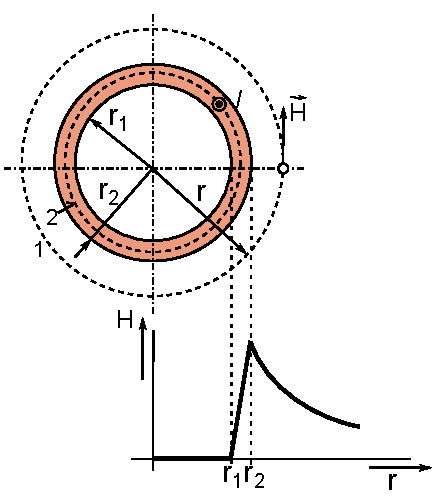
\includegraphics[width=0.8\linewidth]{teo_fig065.pdf}
      \captionof{figure}{K příkladu stanovení intenzity magnetického pole dlouhého dutého válcového 
                vodiče protékaného proudem}
      \label{teo:fig065}
    \par}
    
    Vodič s rovnoměrně rozloženým proudem podle obr. \ref{teo:fig065} je rotačně souměrný podle své
    osy a tedy i jeho magnetické pole je souměrné. Silové čáry jsou soustředné kružnice, vektor
    $\vr{H}$, jenž má směr tečny ke kružnici, je po celé délce kružnice stejně velký. Lze tedy
    snadno použít integrálního tvaru 1. MR (\textbf{zákon celkového proudu})
    
    Pro body ležící vně vodiče obepíná kruhová integrační dráha (vedená po silové čáře 1) celý
    proud vodiče $I$ a platí
    \begin{equation}\label{TEMP:eq_1MR_duty_valec}
      \oint_{\mathcal{C}}\vr{H}d\vr{l} = H\cdot 2\pi r = I
    \end{equation}
    takže intenzita pole je
    \begin{equation}\label{TEMP:eq_H_duty_valec}
      H = \frac{I}{2\pi r}
    \end{equation}
    
    Ve stěně dutého magnetického vodiče jsou silové čáry rovněž kružnice, neboť magnetické pole
    je i zde souměrné. Tyto siločáry však obepínají jen část proudu $I'$ vodiče pro oběh siločáry
    2 platí
    \begin{equation}\label{TEMP:eq_1MR_uvnitr_valce}
      \oint_{\mathcal{C}}\vr{H}d\vr{l} = H\cdot 2\pi r = I' = \pi(r^2-r_1^2)J
    \end{equation}
    kde $J$ je hustota proudu ve vodiči
    \begin{equation}\label{TEMP:eq_J_duty_valec}
      J = \frac{I}{S}= \frac{I}{\pi(r_2^2-r_1^2)}
    \end{equation}
    Ve stěně vodiče je tedy intenzita pole
    \begin{equation}\label{TEMP:eq_H_uvnitr_valce}
      H = \frac{I}{2\pi r}\frac{r^2-r_1^2}{r_2^2-r_1^2}
    \end{equation}
    V dutině vodiče je intenzita rovna nule. Vzhledem k souměrnosti pole by i zde muselo platit
    $\oint_{\mathcal{C}}\vr{H}d\vr{l} = H\cdot 2\pi r$. Protože dráha s poloměrem $r<r_1$ neobepíná
    žádný proud, je $\oint_{\mathcal{C}}\vr{H}d\vr{l} = 0$ a tedy musí byt $H = 0$.
  \end{example}    
\end{mdframed}  
      %------------------------------------------------------------------

      % --------example: $H=f(r)$ souosého kabelu -----------------------
      % \label{TEO:exam013}
      % !TeX spellcheck = cs_CZ
\begin{example}\label{TEMP:ex_koax_H}
  Stanovte intenzitu magnetického pole dlouhého přímého souosého kabelu podle obr.
  \ref{TEMP:fig_exam_koax}. Středním vodičem (\emph{žílou}) prochází proud $I$ a týž proud 
  opačného smyslu prochází vnějším vodičem (\emph{pláštěm}). Proudy jsou rovnoměrně rozloženy po 
  průřezech vodičů. Nakreslete graf průběhu $H = f(r)$ \cite[s.~92]{Dufek1970},
  \cite[s.~195]{Kotlan1999}.
  
  {\centering
   \begin{tabular}{cc}
     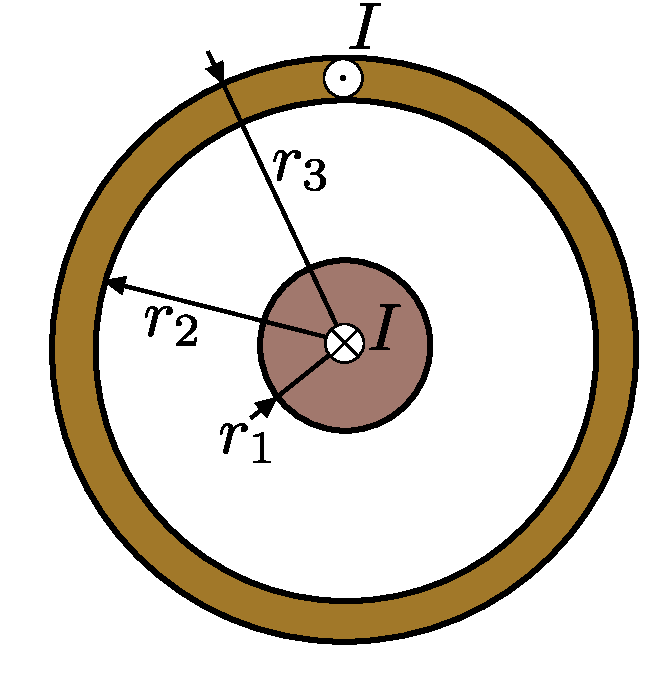
\includegraphics[width=0.4\linewidth]{vypocet_H_sousy_kabel.pdf}   &
     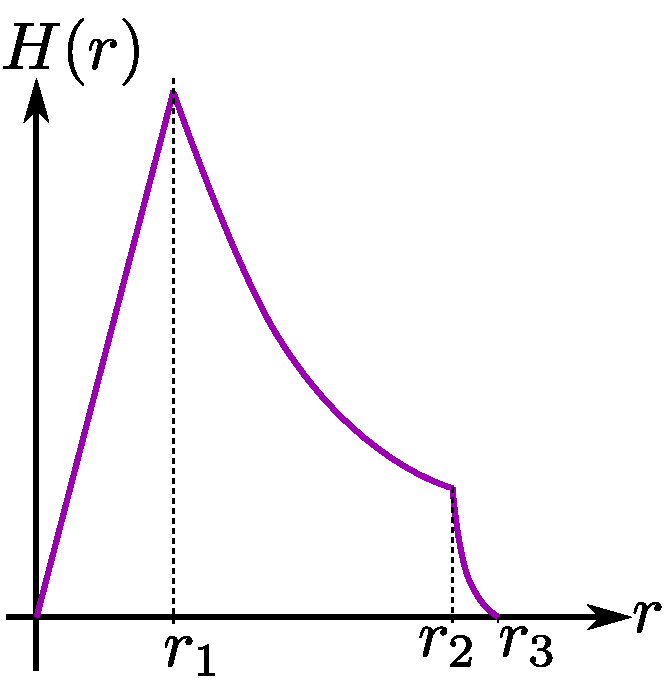
\includegraphics[width=0.4\linewidth]{koax_H_prubeh.pdf}
  \end{tabular}
  \captionsetup{type=figure}
  \captionof{figure}{K příkladu stanovení intenzity magnetického pole dlouhého souosého kabelu 
             protékaného proudem: a) náčrt; b) $H=f(r)$}
  \label{TEMP:fig_exam_koax}
  \par}
  
  \textbf{Řešení}: \newline Rovnici \ref{TEMP:eq_1MR_v_hom_p} aplikujeme na jednotlivé intervaly 
  osově souměrného stacionárního magnetického pole, přičemž se prakticky jedná o superpozici dvou
  polí. V oblasti $r<r_2$ se uplatňuje pouze pole vnitřního válcového vodiče (žíly), pro $r>r_2$ 
  přistupuje souosé pole vnějšího trubkového vodiče.
  \begin{itemize}
    \item Pro oblast $r<r_1$ je vzhledem k 
          \begin{align*}
              % \nonumber to remove numbering (before each equation)
              dI   &= \vr{J}d\vr{S} \\
              I(r) &= \int_S dI = \int_S \vr{J}d\vr{S} = \int_S J\cos\beta dS \\
                   &= \left|\begin{array}{cc}
                               \beta = 0 & H = \text{konst} \\
                             S = \pi r^2 & dS = 2\pi rdr \\
                            \end{array}
                      \right| = J\int_0^r 2\pi rdr = J\pi r^2
          \end{align*}
          hledané řešení 1. MR dáno 
          $$\oint_\mathcal{C}\vr{H}d\vr{l} = H_1 2\pi r = I(r) = J\pi r^2$$ kde celková proudová
          hustota je  $$J = \frac{I}{\pi r_1^2}$$ a tedy $$H_1 = \frac{I}{2\pi r_1^2}\cdot r$$
          
    \item Pro oblast $r_2>r>r_1$ řešíme v podstatě pole vně osamoceného válcového vodiče
          $I(r)$ a tedy $$H_2 = \frac{I}{2\pi r}$$
    \item Pro $r>r_3$ je magnetické pole vytvářeno celým proudem žíly $I$ a příslušnou částí
          proudu pláště $J\pi(r^2 - r_2^2)$, kde proudová hustota $$J =
          \frac{I}{\pi(r_3^2-r_2^2)}$$ má opačnou orientaci oproti proudové hustotě žíly. Pak 
          \begin{align*}
            I(r)                           &= I - I\frac{r^2-r_2^2}{r_3^2-r_2^2} \\
            \oint_\mathcal{C}\vr{H}d\vr{l} &= H_32\pi r = I(r)                   \\          
            H_3                            &= \frac{I}{2\pi r}\left(1 - 
            \frac{r^2 - r_2^2}{r_3^2 - r_2^2}\right) 
          \end{align*}
          Stejný výsledek dostaneme superpozicí opačně orientovaných polí $$H_3 = H'_3 - H''_3 =
          \frac{I}{2\pi r} - \frac{I}{2\pi r}\left(\frac{r^2 - r_2^2}{r_3^2 - r_2^2}\right)$$. 
  \end{itemize}
  Průběh $H(r)$ je na obr. \ref{TEMP:fig_exam_koax}.
\end{example}
  
      %------------------------------------------------------------------

    % -----------Magnetické pole elektrického proudu v diferenciálním tvaru-----------------------
    \subsection{Magnetické pole elektrického proudu v diferenciálním tvaru}
      Nechť je opět magnetické pole vyvoláno konstantním el. proudem $I = \text{konst}$. Jak
      vyplývá z předchozí kapitoly, základním vztahem pro toto pole je \emph{Ampérův zákon}
      $$\oint_{\mathcal{c}}\vec{H_c}\dd{\vec{l}} = I$$  Zvolme za integrační dráhu $c$ obvod malé plošky
      $\Delta S$, jíž prochází proud $\Delta I = J_n \Delta S$, kde $J_n$ je průmět vektoru hustoty
      proudu do směru normály plošky $\Delta S$ (předpokládáme, že ploška $\Delta S$ je dostatečně
      malá, aby se dalo počítat s konstantní hustotou proudu v celém jejím rozsahu)
      \cite[s.~13]{Trnka1972}. Pro zvolený případ platí
      
      \begin{equation}\label{TEMP:eq_amp_z1}
        \oint_{\mathcal{c}}\vec{H_c}\dd{\vec{l}}  =
          J_n \Delta S \rightarrow \frac{1}{\Delta S}\oint_{\mathcal{c}}\vec{H_c}\dd{\vec{l}} = J_n
      \end{equation} 
      
      Pro $\Delta S \rightarrow 0$ zavedeme označení 
      \begin{equation}\label{TEMP:eq_amp_z2}
        \rot{H}  = \frac{1}{\Delta S}\oint_{\mathcal{c}}\vec{H_c}\dd{\vec{l}}  = J_n
      \end{equation}
      
      Rovnice \ref{TEMP:eq_amp_z2} říká, že \emph{rotace vektoru} $\vec{H}$, ($\rot{H}$), jehož
      průmět do určitého směru je roven průmětu vektoru hustoty proudu do tohoto směřu. Z uvedených
      vztahu je patrný fyzikální význam rotace vektoru $\vec{H}$. Je to vektor, jehož velikost je
      rovna oběhovému magnetickému napětí po dráze v rovině kolmé k vektoru hustoty proudu,
      vztaženém k ploše obepínané oběhovou drahou (v nehomogenní poli to platí pro případ, že se
      plocha dráhy blíží k nule).
      
      Při použití pravoúhlé soustavy kartézských souřadnic \(x\), \(y\) a $z$ jsou průměty vektoru
      $\rot{H}$ do jednotlivých os
      \begin{equation}\label{TEMP:eq_amp_z3}
        \textsf{rot}_x\vec{H} = J_x,   \quad
        \textsf{rot}_y\vec{H} = J_y,   \quad
        \textsf{rot}_z\vec{H} = J_z    
      \end{equation}      
      Průmět $\textsf{rot}_x\vec{H}$ je dán oběhovým magnetickým napětím po obvodu plošky
      \(\dd{y}\dd{z}\) a platí
      \begin{align*}
        \textsf{rot}_x\vec{H} 
        &=\frac{1}{\dd{y}\dd{z}}\oint_{\mathcal{c}}\vec{H_c}\dd{\vec{l}} =               \nonumber\\
        &=\frac{1}{\dd{y}\dd{z}}\cdot\Biggl[\Biggr.\left[H_y\dd{y} 
         +\left(H_z + \pder{Hz}{y}\dd{y}\right)\dd{z}\right]                             \nonumber\\     
        &-\left[\left(H_y-\pder{H_y}{z}\dd{z}\right)\dd{y}-H_z\dd{z}\right]\Biggl.\Biggr]\nonumber\\
        &=\pder{H_z}{y}\dd{y}\dd{z} - \pder{H_y}{z}\dd{y}\dd{z}                          \nonumber\\    
        &=\pder{H_z}{y} - \pder{H_y}{z} = J_z
      \end{align*}       
      
      \luagraphic[0.8]{teo_fig062.pdf}{K odvození pojmu \(\textsf{rot}_z\vec{H}\)}{teo:fig062}
         
      tedy dostáváme
      \begin{subequations}
        \begin{align}\label{TEMP:eq_amp_z5}
          \textsf{rot}_x\vec{H} &= \pder{H_z}{y} - \pder{H_y}{z} = J_x       \\
          \textsf{rot}_y\vec{H} &= \pder{H_x}{z} - \pder{H_z}{x} = J_y       \\
          \textsf{rot}_z\vec{H} &= \pder{H_y}{x} - \pder{H_x}{y} = J_z            
        \end{align}    
    \end{subequations}    
      Pro \emph{pravoúhlé souřadnice} $x, y, z$ můžeme tedy vztah $\rot{H} = \vec{J}$ rozepsat na
      tvar
      \begin{align*}
        \textsf{rot}\vec{H} 
          &= \vec{i}\,\textsf{rot}_x\vec{H} + 
             \vec{j}\,\textsf{rot}_y\vec{H} +
             \vec{k}\,\textsf{rot}_z\vec{H}                                    \\
          &= \vec{i}\left(\pder{H_z}{y} - \pder{H_y}{z}\right) +               \\
          &+ \vec{j}\left(\pder{H_x}{z} - \pder{H_z}{x}\right) +               \\
          &+ \vec{k}\left(\pder{H_y}{x} - \pder{H_x}{y}\right)                 \\  
          &= \vec{i}\,J_x + \vec{j}\,J_y + \vec{k}\,J_z = \vec{J}.
      \end{align*}          
      
      Rotaci vektoru $\rot{H}$ můžeme též symbolicky vyjádřit vektorovým součinem Hamiltonova
      operátoru a vektoru $\vec{H}$
      \begin{align*}
        \rot{H} &= \nabla\times\vec{H}                                                      \\                                           
                &= \left(\vec{i}\,\pder{ }{x} + 
                   \vec{j}\,\pder{ }{y} + \vec{k}\,\pder{ }{z}\right)                       \\
                & \times(\vec{i}\,H_x + \vec{j}\,H_y + \vec{k}\,H_z)
      \end{align*}
      nebo také determinantu
      \begin{equation}\label{TEMP:eq_amp_z8}
        \rot{H} = \begin{vmatrix}
                    \vec{i}       & \vec{j}      & \vec{k}      \\
                    \pder{ }{x}  & \pder{ }{y} & \pder{ }{z} \\ 
                    H_x          & H_y         & H_z         \\
                  \end{vmatrix}      
      \end{equation}  
      \emph{cylindrických souřadnic} $r$, $\varphi$, $z$:
      \begin{align}\label{TEMP:eq_amp_z9}
        \textsf{rot}_r\vec{H}       
          &= \frac{1}{r}\pder{H_z}{\varphi} - \pder{H_\varphi}{z} = J_r           \nonumber \\ 
        \textsf{rot}_\varphi\vec{H} 
          &= \pder{H_r}{z} - \pder{H_z}{r}                        = J_\varphi     \nonumber \\
        \textsf{rot}_z\vec{H}       
          &= \frac{1}{r}\left[\pder{ }{r}
             \left(rH_\varphi\right)-\pder{H_r}{\varphi}\right]   = J_z
      \end{align} 
      \emph{sférických souřadnic} $r$, $\varphi$, $\vartheta$ 
      \begin{align}\label{TEMP:eq_amp_z10}
        \textsf{rot}_r\vec{H}        
           &= \frac{1}{r\sin\vartheta}\left[\pder{ }{\vartheta}(H_\varphi\sin\vartheta) - 
              \pder{H_\vartheta}{\varphi}\right]                     = J_r           \nonumber \\ 
        \textsf{rot}_\varphi\vec{H}   
           &= \frac{1}{r}\left[\pder{ }{r}(rH_\vartheta) - 
              \pder{H_r}{\vartheta}\right]                           = J_\varphi     \nonumber \\
        \textsf{rot}_\vartheta\vec{H} 
           &= \frac{1}{r\sin\vartheta}\left[\pder{H_r}{\varphi} -
              \pder{ }{r}\left(rH_\varphi\sin\vartheta\right)\right] = J_\vartheta    
    \end{align} 
      Podobně jako v elektrickém poli vyjadřujeme vztah $\oint\vec{D}\dd{\vec{S}} = Q$ vztahem 
      $\diver{D}
      = \rho$, tak i v magnetickém poli vyjadřujeme vztah $\oint\vec{B}\dd{\vec{S}} = 0$ vztahem
      $\diver{D} = 0$, nebo též v kartézských souřadnicích \(x\), \(y\) a $z$ jako $$\diver{D} =
      \nabla\cdot\vec{B} = \pder{B_x}{x} + \pder{B_y}{y} + \pder{B_z}{z} = 0$$
                     
    % ----------------Rovnice pro magnetický potenciál -------------------------------------------
    \subsection{Rovnice pro magnetický potenciál}
      V regulárních bodech lineárního homogenního izotropního magnetika platí pro $\varphi_m$
      \textbf{Laplaceova rovnice}
      \begin{equation}\label{TEMP:eq_varphi_m_laplace}
        \Delta\varphi_m = 0
      \end{equation}      
      Důkaz plyne z rovnice $\diver{B} = 0$ a rovnice $\vec{B} = \mu\vec{H}$: $$\diver{B} =
      \textsf{div}\mu\vec{H} = \textsf{div}\mu(-\textsf{grad}\varphi_m).$$ Pro $\mu = \text{konst}$
      dostáváme $\textsf{div}\textsf{grad}\varphi_m = 0$, což je rovnice
      \ref{TEMP:eq_varphi_m_laplace}.
      
      Na rozhraní mezi dvěma magneticky různými prostředími neplatí Maxwellovy rovnice v
      diferenciálním tvaru a tedy ani Laplaceova rovnice \ref{TEMP:eq_varphi_m_laplace}. Podmínky 
      pro $\vec{H}$ a $\vec{B}$ na rozhraní vyjádříme pomocí skalárního magnetického potenciálu
       \begin{align}\label{TEMP:eq_mag_U_rozhrani}
         \varphi_{m1}                 &= \varphi_{m2} \\
         \mu_1\pder{\varphi_{m1}}{n}  &= \mu_2\pder{\varphi_{m2}}{n} 
       \end{align}
      kde $\pder{}{n}$ jsou derivace ve směru normály k rozhraní. 
    
    \subsubsection{Vektorový magnetický potenciál}
      V elektrostatice jsme pro usnadnění mnohých problémů zavedli skalární elektrický potenciál -
      lze jej zavést vždy, neboť elektrostatické pole je vždy potenciální. Magnetické pole je však
      obecně vírové. Lze jej popsat skalárním potenciálem jen ve speciálních případech, tj.
      jestliže je polem potenciálním. Obecně je však zavedení skalárního potenciálu nepřípustné.
      Lze i pak zavést nějakou veličinu (analogickou skalárnímu potenciálu), s níž by se pracovalo
      snáze, než přímo s vektory pole?
      
      Dříve než definujeme vektorový magnetický potenciál, zopakujme zavedení skalárního potenciálu
      v elektrostatice. Vyjdeme z 2. MR a z rovnice známé z vektorové analýzy: $$\rot{E} = 0 \quad
      \text{a} \quad \textsf{rot}\,\textsf{grad}\varphi_m = 0.$$
      
      V magnetickém poli vyjdeme ze 4. MR a z jiné identity pro vektorovou funkci $\vec{A}$, známe z
      vektorové analýzy: $$\diver{B} = 0 \quad \text{a} \quad \textsf{div}\textsf{rot}\vec{A} =
      0$$ odtud
        \begin{equation}\label{TEMP:eq_B_rotA}
          \vec{B} = \rot{A}.
        \end{equation}       
               
%} % tikzset
%~~~~~~~~~~~~~~~~~~~~~~~~~~~~~~~~~~~~~~~~~~~~~~~~~~~~~~~~~~~~~~~~~~~~~~~~~~~~~~~~~~~~~~~~~~~~~~~~~~
  % !TeX program = lualatex
% !TeX root = luaking.tex
% !TeX encoding = UTF-8
% !TeX spellcheck = cs_CZ
%---------------------------------------------------------------------------------------------------
% file magn1ch01.tex
\graphicspath{{../src/TEO/img/}}
%---------------------------------------------------------------------------------------------------
%====================Kapitola: Základní zákony elektromagnetismu====================================
\setchaptertoc
\chapter{Základní zákony elektromagnetismu}\label{teo:IchapII}
  V této teoreticky změřené kapitole budou shrnuty základní fyzikální zákony, kterými se řídí
  elektromagnetické jevy a jejichž znalost bude nezbytná při studiu následujících praktičtěji
  zaměřených kapitol. Mezi nejdůležitější patří zákon elektromagnetické indukce. Velký praktický
  význam má jeho zobecnění i pro případy nejsložitější, jakými jsou \emph{nelineární} a navíc
  \emph{parametrické} magnetické obvody. Důležitým pojmem je \emph{spřažený} magnetický tok cívky.
  Pro hlubší pochopení všech zákonitostí bude vhodné upozornit na \emph{topologické vlastnosti}
  elektromagnetického pole. Ukazuje se totiž, že topologický přístup je velice užitečným a silným
  nástrojem, který významně usnadňuje pochopení \wikiMaxwellEq se všemi jejich důsledky
  \cite[s.~6]{Patocka4}. Topologii elektromagnetického pole je proto věnována celá kapitola
  \ref{teo:IchapIII}
  
  \section{Zákon elektromagnetické indukce}\label{teo:IchapIIsecI}
    Základní veličinou pro popis magnetických polí a jejich účinků je \emph{vektor magnetické
    indukce} \(\vec{B}\). Dle soustavy SI je jednotkou magnetické indukce \emph{tesla} \([T]\) a
    projevuje se silovými účinky na vodiče protékané proudy a indukováním napětí při jeho změně.

    Je proto dobře měřitelný. První rovnice (Ampérův zákon) ze souboru Maxwellových rovnic určuje
    rovnost oběhového integrálu magnetické indukce po uzavřené křivce proudům protékaných vodiči,
    jež jsou touto křivkou uzavřeny.
    \begin{equation}\label{TEO:eq101}
      \oint_l \vec{B} \cdot \vec{\dd{l}} = \sum I
    \end{equation}
    
    \luagraphic[0.4]{teo_fig034.pdf}{Elektrický proud ve vodiči způsobuje vznik magnetické pole v 
      jeho okolí.}{teo:fig034}

    Obrázek \ref{teo:fig034} ilustruje fakt, že elektrické proudy jsou vždy obklopeny 
    magnetickými poli. Tato pole se dají zesílit cívkou s magnetickým jádrem. Na tomto jevu je 
    založen jeden z elementárních principů elektrotechniky.    
       
    \begin{mdframed}[style=mdnote]
      Jaký je vztah jednotky magnetické indukce k ostatním základním jednotkám soustavy \textbf{SI}? 
      \begin{align*}
        \SI{1}{\tesla}
          &= 1\frac{V\cdot s}{m^2} = 1\frac{N}{A\cdot m} = 1\frac{Wb}{m^2}          \\
          &= 1\frac{kg}{C\cdot s} = 1\frac{kg}{A\cdot s^2} = 1\frac{N\cdot s}{C \cdot m}
      \end{align*}
    \end{mdframed}
    
    Při odvozování matematického modelu transformátoru se obvykle vychází ze zákona 
    \textbf{elektromagnetické indukce}, který říká, že \emph{časová změna magnetického pole vytvoří 
    vírové pole elektrické}:
    \begin{equation}\label{es:eq_ind_z}
      \oint_l \vec{E} \cdot \dd{\vec{l}} = - \der{\Psi}{t}
    \end{equation}
     
    Základní laboratorní experimenty, vedoucí k odhalení existence tohoto zákona, uskutečnil 
    \textsc{M. Faraday}\footnote{Michael Faraday (1791 - 1867), samouk, zakladatel klasické 
    elektrodynamiky, vynikající experimentátor: Zavedl pojem fyzikálního prostorového pole pomocí 
    siločár, tzv. ''trubic''} v roce 1831. Matematickou formulaci \emph{indukčního zákona} v podobě 
    rovnice
    \begin{equation}\label{TEO:eq102}
      u(t) = - \frac{d\Psi(t)}{\dd{t}}
    \end{equation} 
    stanovil již on sám, postupně význam zákona formálně upřesňovali další badatelé např. \textsc{F.
    E. Neumann}\footnote{Franz Ernst Neumann (1798 - 1895), teoretický fyzik, matematik, mineralog.
    Definoval pojem magnetický vektorový potenciál, formuloval Neumannův vzorec pro vzájemnou
    indukčnost dvou smyček. Učitel G. R. Kirchhoffa.} kolem roku 1845. Konečné znění Maxwellovy
    teorie včetně formulace indukčního zákona do podoby II. Maxwellovy rovnice budoval \textsc{J. C.
    Maxwell}\footnote{James Clark Maxwell (1831 - 1879), teoretický fyzik, působil na Trinity
    College university v Cambridge, na King's College v Londýně, posléze první ředitel Cavendishovy
    laboratoře na univerzitě v Cambridge. Původně se zabýval teoretickou mechanikou a kinetickou
    teorií plynů. Soustavu čtyř Maxwellových rovnic odvodil především na základě
    mechanicko-elektrických analogií.} velmi pozvolna, v období 1855 až 1873. Z historického pohledu
    je zajímavé a důležité, že přesné \emph{kvantitativní} experimenty s elektromagnetickou indukcí
    byly v té době uskutečnitelné pouze pomocí \wikiGalvanometer. Lze odhadnout, že nebýt tohoto
    přístroje, přesná matematická formulace indukčního zákona by se pravděpodobně opozdila o několik
    let. Kupodivu, z psychologického hlediska je i v současnosti velmi vhodné vysvětlit princip
    indukčního zákona pomocí historických pokusů s balistickým galvanometrem.
    
    \subsection{Pokusy s balistickým galvanometrem}
      Jako každý elektromagnetický měnič energie (tj. motor), obsahuje i \emph{magnetoelektrické
      měřicí} ústrojí galvanometru dva akumulátory energie: moment setrvačnosti \(J\) otoč\-né 
      části a indukčnost cívky \(L\). Jedná se tedy o kmitavou soustavu 2. řádu. Každou takovou 
      soustavu lze kriticky, případně nadkriticky tlumit - především zařazením tlumicího odporu 
      vhodné velikosti do série s měřicím systémem (tlumení vlivem mechanického tření je úmyslně 
      konstrukčně potlačeno na zanedbatelnou úroveň). Balistický galvanometr je cíleně konstruován 
      s velkým momentem setrvačnosti \(J\) a s malou tuhostí \(k_d\) direkčních pružin, aby měl 
      dlouhou dobu kmitu \(T_G = 2\pi\sqrt{J/k_d}\) několik sekund. Proteče-li galvanometrem krátký 
      proudoý impuls \(i(t)\) o celkové délce \(t_i\) podle obr. \ref{teo:fig036}, pak lze snadno 
      dokázat, že za předpokladu \(t_i\ll T_G\) je první maximální výchylka \(\alpha_{max}\) 
      tlumeného pohybu ukazatele přímo úměrná celkovému náboji \(Q\) proudového impulsu podle 
      rovnice 
      \begin{equation}\label{TEO:eq103}
        \alpha_{max} = k_b Q = k_b\int_0^{t_i} i(t)\dd{t},
      \end{equation}
      kde \(k_b\) je \emph{balistická konstanta} použitého galvanometru. Balistický galvanometr tedy
      pracuje jako \emph{integrátor} proudu v přesném matematickém smyslu. 
      
      \luagraphic[1]{teo_fig036.pdf}{Příklad krátkého proudového impulsu prošlého balistickým 
        galvanometrem.}{teo:fig036}
  
      Uvažujme experiment uspořádaný podle obr. \ref{teo:fig037}. V uzavřeném obvodu
      galvanometru se nachází celkový odpor \(R\) a tuhá samonosná cívka v podobě kruhového závitu,
      připojená na dlouhé ohebné zkroucené přívody. Husté zkroucení zajišťuje, že do samotných
      přívodů se nemůže indukovat žádné napětí, pohybuje-li se cívka v magnetickém poli 
      permanentního magnetu. Při rychlém přesunu z polohy \emph{1} do vzdálené polohy \(\infty\) 
      klesne v cívce magnetický tok na nulu, časová změna toku zapříčiní vznik indukovaného napětí, 
      napětí protlačí obvodem proudový impuls odpovídající přibližně obr. \ref{teo:fig036}.
      
      \luagraphic[0.8]{teo_fig037.jpg}{Uspořádání experimentálního pracoviště s balistickým 
        galvanometrem}{teo:fig037}
      
      Za předpokladu kritického nebo nadkritického tlumení má odpor \(R\) relativně velkou hodnotu. 
      Proto lze s dobrou přesností zanedbat vnitřní indukčnost měřicího systému galvanoměru a 
      uvažovat, že celé napětí \(u(t)\), indukované v cívce při jejím pohybu, spočine pouze na 
      odporu. V uzavřeném okruhu o celkovém odporu \(R\) pak platí Ohmův zákon ve tvaru
      \begin{equation}\label{TEO:eq104}
        i(t)=\frac{u(t)}{R}.
      \end{equation}    
      Dosadíme-li rovnici \ref{TEO:eq104} do \ref{TEO:eq103}, po úpravě získáme vztah
      \begin{equation}\label{TEO:eq105}
       \int_0^{t_i}u(t)\dd{t}=\frac{\alpha_{max}R}{k_b}.
      \end{equation}     
      Experimentálně je možno dospět ke dvěma stěžejním poznatkům:
      \begin{itemize}
        \item Při přesunu cívky z polohy \emph{1} do polohy \(\infty\) nezávisí výchylka
              \(\alpha_{max}\) na \emph{rychlosti pohybu}. (Za předpokladu \(t_i\ll T_G\), což je
              omezení dané nedokonalostí přístroje a nijak nesouvisí se zkoumaným jevem.)
        \item Při přesunu cívky z polohy \emph{1} do polohy \(\infty\) zůstává součin
              (\(\alpha_{max}\times R\)) stále \emph{konstantní}, měníme-li úmyslně velikost odporu
              \(R\). To jest: při k-násobném zvýšení odporu klesne výchylka k-krát a naopak. 
      \end{itemize}
  
      V poloze „1“ prochází plochou cívky magnetický tok \(\Psi\). V poloze „\(\infty\)“ je zřejmě
      magnetický tok cívky nulový, tedy \(\Psi_\infty = 0\). S ohledem na rovnici
      (\ref{TEO:eq105}) lze pak oba experimentální poznatky interpretovat jediným možným
      způsobem:
       \begin{equation}\label{TEO:eq106}
       \int_0^{t_i}u(t)\dd{t}=\text{konst}=\Psi-\Psi_\infty=\Psi.
      \end{equation}    

      Experiment lze opakovat s cívkami libovolných rozměrů, tvarů i počtů závitů. Výsledky budou
      kvalitativně stejné. Veličina \(\Psi\) se nazývá \emph{spřažený magnetický tok cívky}. Je to 
      míra interakce cívky s magnetickým polem, které spojitě prostupuje celou plochou cívky. 
      Rovnici (\ref{TEO:eq106}) lze vyjádřit slovně: Spřažený magnetický tok cívky je úměrný 
      časovému integrálu svorkového napětí na zkoumané cívce. Je určitě výhodné zvolit jedničku 
      jako konstantu úměrnosti mezi tokem \(\Psi\) a integrálem napětí. \emph{Pak bude velikost 
      spřaženého toku přímo rovna integrálu napětí}. Určitý integrál v rovnici 
      (\ref{TEO:eq106}) lze nahradit integrálem neurčitým, pak je ale nutno přidat obecnou 
      počáteční integrační konstantu \(\Psi_0\)
      v newtonovském smyslu. Získáme tak zákon elektromagnetické indukce (indukční zákon) v
      integrálním tvaru
      \begin{equation}\label{TEO:eq107}
       \Psi(t) = \Psi_0 + \int u(t)\dd{t} \quad [Wb;\, V,\; s].
      \end{equation}   
    
    Z rovnice (\ref{TEO:eq107}) plyne, že jednotka magnetického toku Weber\footnote{Wilhelm Eduard
    Weber (1804-1891), teoretický fyzik, působil na univerzitách v Gottingenu a v Lipsku. Zakladatel
    předrelativistické elektrodynamiky. Určil totiž silu mezi náboji v závislosti nejen na
    vzdálenosti, ale i na rychlosti a zrychlení, jeho teorie je ale platná pouze pro \(v \ll c\).
    Blízký spolupracovník Gausse.} má rozměr \([Vs]\), Budeme-li obě strany rovnice derivovat podle
    času, rovnost tím neporušíme. Získáme tak ryze matematickou cestou indukční zákon v
    diferenciálním tvaru
    \begin{equation}\label{TEO:eq108}
     u(t) = \frac{d\Psi(t)}{\dd{t}}, \quad \text{resp.} \quad  u(t) = -\frac{d\Psi(t)}{\dd{t}}.
    \end{equation}   
    Obě rovnice (\ref{TEO:eq108}a), (\ref{TEO:eq108}b) se liší znaménkem \(+\) nebo \(-\) na pravé
    straně. Volba znaménka souvisí s domluvou, který režim cívky považujeme za základní: zda režim
    \emph{spotřebičový} podle rovnice (\ref{TEO:eq108}a), nebo režim \emph{zdrojový} podle rovnice
    (\ref{TEO:eq108}b). Oba režimy jakéhokoli dvojpólu jsou totiž jednoznačně definovány vzájemnou
    orientací napětí a proudu podle obr. \ref{teo:fig039}. Odpor nemůže nikdy pracovat jako zdroj,
    proto slouží jako „normál“ definující \emph{spotřebičovou} orientaci svorkových veličin. Oba
    režimy cívky se liší níže popsaným způsobem.

    \begin{figure}[ht!]
      \centering  
      \subcaptionbox{Odpor je vždy spotřebičem     \label{teo:fig039a}}
        {\luafigure[0.4]{teo_fig039a.pdf}}                    
      \subcaptionbox{Cívka ve spotřebičovém režimu \label{teo:fig039b}}
        {\luafigure[0.4]{teo_fig039b.pdf}}         \\               
      \subcaptionbox{Cívka ve zdrojovém režimu     \label{teo:fig039c}}
        {\luafigure[0.4]{teo_fig039c.pdf}}
      \caption{Vzájemná orientace okamžité hodnoty proudu a napětí ve spotřebičovém a zdrojovém 
               režimu.} 
      \label{teo:fig039}
    \end{figure}
        
    \textbf{Spotřebičový režim:}
    \begin{itemize}[noitemsep]
      \item Orientace svorkového napětí \(u(t)\) je vůči proudu \(i(t)\) souhlasná. Platí rovnice
            (\ref{TEO:eq108}a).
      \item Cívka je připojena na zdroj napětí\(u(t)\), odebírá z něj proud \(i(t)\), tedy odebírá
            ze zdroje elektrickou energii a chová se jako spotřebič. Tuto energii přeměňuje na
            energii magnetického pole.
      \item Mezi směrem proudu a směrem toku platí \emph{pravidlo pravé ruky}, PPR.           
    \end{itemize}
    
    \textbf{Zdrojový režim:}
    \begin{itemize}[noitemsep]
      \item Orientace svorkového napětí u(t) je vůči proudu i(t) nesouhlasná. Platí rovnice
            (\ref{TEO:eq108}b).
      \item Cívka je vložena do proměnného magnetického pole \(B(t)\), na jejích svorkách vzniká
            indukované napětí \(u(t)\) (zastaralý výraz: „elektromotorická síla“). Z cívky se stal
            zdroj elektrického napětí u(t), tj. generátor. Připojíme-li na svorky odporovou zátěž,
            začne do ní generátor dodávat elektrickou energii.\footnote{Faraday s Maxwellem se znali
            osobně a po dohodě pokládali zdrojový režim cívky za základní, tedy pracovali s rovnicí
            (\ref{TEO:eq108}b). Maxwell navíc pracoval s pojmem „electromotive force \(P\)‘, který
            svým významem přesně odpovídal dnešní „intenzitě elektrického pole. Postupem času byl
            doslovně přeloženému výrazu „elektromotorická síla“ nešťastně přiřazen v české i
            zahraniční literatuře význam „napětí“, což ještě více zvýšilo zmatek. Proto je rozumné
            výraz „elektromotorická síla“ vůbec nepoužívat.}
    \end{itemize}

    \luagraphic[1]{teo_fig038.jpg}{Princip transformátoru. Primární cívka pracuje ve
    spotřebičovém režimu (PPR), sekundární cívka ve zdrojovém režimu (PLR)}{teo:fig038}

    Z uvedených skutečností lze učinit následující závěr. Volba znaménka v rovnicích
    (\ref{TEO:eq108}a, b) je věcí dohody, ale pouze v tom smyslu, zda zvolíme za základní režim
    spotřebičový či zdrojový\footnote{Ojediněle se v literatuře, např. v [5], vyskytne názor, že
    znaménko v rovnicích (\ref{TEO:eq108}a, b) je určeno tím, zda je cívka navinuta pravotočivě nebo
    levotočivé. To je chybné tvrzení. Pravotočivost či levotočivost cívky naprosto nijak nesouvisí
    se schopnosti cívky pracovat ve zdrojovém nebo spotřebičovém režimu.}. Například při analýze
    měničů ve výkonové elektronice je ustáleným zvykem zvolit označení proudu a napětí na
    indukčnosti podle obr. \ref{teo:fig039b}. Bez ohledu na tuto volbu musíme v konkrétní situaci
    vždy pečlivě rozlišovat, ve kterém režimu se cívka skutečně nachází. Příklad: primární cívka
    transformátoru se nachází vždy ve spotřebičovém režimu, sekundární cívka vždy ve zdrojovém
    režimu. Se zdrojovým či spotřebičovým režimem úzce souvisí \emph{Lenzův
    princip}\footnote{Heinrich Lenz (1804-1865), estonský fyzik, působil na univerzitě v Petrohradu.
    Princip po něm pojmenovaný objevil r. 1833.}. Jedná se o zvláštní případ obecnějšího přírodního
    principu, vyjádřitelného jako „zákon akce a reakce“. V elektromagnetismu má zákon následující
    tvar:

    Lenzův princip: Proud indukovaný v uzavřené vodivé smyčce vyvolá magnetické pole, které působí
    vždy proti původnímu budicímu poli, díky němuž indukovaný proud vznikl.

    Všimněme si, že zmíněná „uzavřená vodivá smyčka“ se nachází \emph{zdrojovém režimu}: je vložena
    do magnetického pole, indukuje se v ní napětí \(u(t)\), které protlačí vodivým obvodem proud
    \(i(t)\). Proud má ve \emph{zdrojovém režimu} takový směr, že působí proti budicímu magnetickému
    poli. Příkladem je již zmíněná sekundární cívka transformátoru podle Obr. /./-*/« nebo uzavřená
    smyčka vířivého proudu ve vnitřním prostoru transformátorového plechu podle Obr. 1.1-5.

    \luagraphic[1]{teo_fig040.jpg}{Vznik vířivého proudu uvnitř elektricky vodivého
    transformátorového plechu. Budicí cívka pracuje ve spotřebičovém režimu (PPR). Elementární
    smyčka vířivého proudu odpovídá sekundárnímu vinutí a pracuje ve zdrojovém režimu
    (PLR).}{teo:fig040}

    Integrací rovnice (\ref{TEO:eq108}a) lze zpětně dojít k integrálnímu tvaru
    (\ref{TEO:eq107}). Je nutno zdůraznit, že obě rovnice jsou naprosto rovnocenné, navzájem
    převoditelné, obě nesou stejné množství informace, žádná není důležitější než druhá. Je
    pravdou, že z psychologického pohledu je indukční zákon snáze pochopitelný v
    \emph{diferenciálním} tvaru (\ref{TEO:eq108}). Pro hluboké porozumění magnetickým jevům
    je však nezbytné uvědomit si především jeho \emph{integrální} podobu (\ref{TEO:eq107})
    se všemi matematickými důsledky:
    \begin{itemize}
      \item Spřažený tok je roven integrálu napětí. Zákon platí \emph{univerzálně}, bez ohledu na
            \emph{linearitu} či \emph{nelinearitu} magnetického obvodu. Rovnice
            (\ref{TEO:eq107}) totiž definuje funkční závislost \(\Psi=\Psi(u)\) mezi tokem a
            napětím, nikoli závislost \(\Psi=\Psi(i)\) mezi \emph{tokem a proudem}.  Případná
            nelinearita se totiž týká výlučně závislosti \(\Psi=\Psi(i)\), a tudíž nijak nenarušuje
            platnost rovnice (\ref{TEO:eq107}).
      \item Z předchozího bodu plyne, že v obecném \emph{nelineárním} případě není tok \(\Psi\)
            přímo úměrný proudu \(i\). Přímá úměra \(\Psi = Li\) totiž platí pouze ve zvláštním
            případě \emph{lineárního} magnetického obvodu.
      \item Rovnice (\ref{TEO:eq107}) platí ve spotřebičovém i generátorovém režimu cívky.
            Problém se znaménkem zůstává stejný jako u rovnic (\ref{TEO:eq108}).
      \item V uzavřené \emph{supravodivé} smyčce platí vždy \(u = 0\), i když jí teče konstantní
            ss. proud. Neurčitý integrál v rovnici (\ref{TEO:eq107}) má pak nulovou hodnotu
            \(\int0\dd{t}=0\), a zřejmě tedy platí \(\Psi(t)=\Psi_0\), kde \(\Psi_0\) je
            \emph{libovolná} počáteční integrační konstanta. Fyzikálně má konstanta význam
            počátečního toku, který je v cívce naintegrován z předchozích dějů. Případ
            \(\Psi_0\neq0\) odpovídá nabuzenému supravodivému magnetu, jehož tok \(\Psi(t)=\Psi_0
            = \text{konst.}\) se s časem nemění. Nabuzený supravodivý magnet se proto chová jako
            \emph{permanentní} magnet. Případ \(\Psi_0 = 0\) odpovídá magnetickému stínění pomocí
            \emph{závitu nakrátko}, např. tzv. Faradayova klec, nebo stínění koaxiálního kabelu
            podle obr. \ref{teo:fig041}. Každé oko \textbf{a-b-c-d} stínícího pláště
            tvoří „supravodivý“ závit nakrátko, v němž platí \(u = 0\), tedy \(\Psi=\int0\dd{t}=0\).
            Proto se do vnitřního prostoru ohraničeného pláštěm nemůže zvenčí dostat žádné
            \emph{střídavé} rušivé magnetické pole (jedině pole \emph{stejnosměrné} \(\Psi_{ss}\),
            ale to je neškodné, protože nezpůsobuje vznik rušivého napětí ve středním vodiči
            kabelu; derivace konstanty je totiž nulová: \(u(t)=\frac{d\Psi_{ss}}{\dd{t}}=0\)).
    \end{itemize}

    Na otázku „Proč je magnetický tok úměrný integrálu napětí?“ lze odpovědět pouze následujícím
    způsobem: „Protože je to jeden ze základních zákonů přírody, jehož správnost se nepodařilo
    experimentálně nikdy vyvrátit, nýbrž vždy pouze potvrdit.“ Deduktivní odvození indukčního zákona
    z vyšších přírodních zákonitostí není na úrovni klasické fyziky možné, není uskutečnitelné ani
    na vyšší úrovni \emph{kvantové elektrodynamiky}\footnote{Za objev kvantové elektrodynamiky
    obdržel Richard P. Feynman (1918-1988) Nobelovu cenu v r. 1965 (Feynmanovy fázorové diagramy a
    Feynmanův dráhový integrál; nositelé elektromagnetických sil jsou fotony). Vynikající teoretický
    fyzik, ale i praktik. Celoživotně působil na kalifornském technickém institutu. Během druhé
    světové války byl členem týmu pracujícího na vývoji americké atomové bomby v Los Alamos (projekt
    Manhattan).}. Za povšimnutí stojí, že v diferenciální formě (\ref{TEO:eq108}) nebylo přesné
    kvantitativní ověření indukčního zákona v době objevu proveditelné s ohledem na možnosti
    tehdejšího přístrojového vybavení. Experiment v nehomogenním poli podle obr. \ref{teo:fig037} by
    byl i v současnosti velmi těžko vyhodnotitelný. Naopak, ověření v integrálním tvaru je velmi
    snadné\footnote{V současnosti by byl balistický galvanometr nahrazen operačním zesilovačem
    zapojeným jako integrační zesilovač. Ten by zpracovával signál ze snímače proudu, např. z
    proudového bočníku. Po odeznění proudového impulsu by na výstupu zesilovače zůstalo
    naintegrováno určité konstantní napětí, jehož velikost by analogicky odpovídala maximální
    výchylce \(\alpha_{max}\) galvanometru.} . To opravňuje k domněnce vyslovené v historickém úvodu
    kapitoly.

    \begin{figure}[ht!]
      \centering  
      \subcaptionbox{\label{teo:fig041a}}{\luafigure[0.4]{teo_fig041a.jpg}}                    
      \subcaptionbox{\label{teo:fig041b}}{\luafigure[0.4]{teo_fig041b.jpg}}  
      \caption{Plášť koaxiálního kabelu. Každé oko \textbf{a-b-c-d} tvoří závit nakrátko.} 
      \label{teo:fig041}
    \end{figure}
      
    Supravodivá cívka podle obr. \ref{teo:fig042} začne být v okamžiku \(t = 0\)
    napájena ideálním zdrojem napětí \(u(t)\). Později na ni začne působit vnější magnetické pole
    přibližujícího se permanentního magnetu. Jaký vliv bude mít PM na velikost spřaženého toku
    cívky?
    
    Odpověď plyne přímo z rovnice (\ref{TEO:eq107}): \(\Psi(t) = \Psi_0 +\int u(t)\dd{t}\).
    
    Ze zadání příkladu vyplývá, že počáteční integrační konstanta je nulová. Neurčitý integrál je
    možno nahradit integrálem určitým. Velikost spřaženého toku je \emph{tvrdě definována}
    přiloženým napětím, tedy hodnotou určitého integrálu. Proto externí magnetické pole 
    \emph{nemůže} spřažený tok cívky nijak změnit. Ideální napěťový zdroj má \emph{nulový} 
    vnitřní odpor. Proto se supravodivá cívka napájená tímto zdrojem stále chová jako supravodivý
    závit nakrátko, do něhož nemůže vniknout žádná siločára externího magnetického pole.
    
    \begin{figure}[ht!]
      \centering  
      \subcaptionbox{\label{teo:fig042a}}{\luafigure[0.41]{teo_fig042a.jpg}}                    
      \hspace{1em}
      \subcaptionbox{\label{teo:fig042b}}{\luafigure[0.45]{teo_fig042b.jpg}}        \\               
      \subcaptionbox{\label{teo:fig042c}}{\luafigure[0.41]{teo_fig042c.jpg}}
      \caption{K příkladu, a) Supravodivá cívka je napájená ideálním napěťovým zdrojem, b) Později
               na ni začne působit externí pole pohybujícího se magnetu, c) Náhradní zapojení.} 
      \label{teo:fig042}
    \end{figure}
  
    Jev lze vysvětlit následovně. Pohybující se magnet indukuje v cívce přídavné indukované napětí
    \(u(t)\). Toto napětí se přičte k napětí napájecímu a způsobí změnu proudu \(\Delta i(t)\)
    tekoucího cívkou. Podle Lenzova principu začne tento přídavný proud působit proti poli PM.
    Přídavný proud \(\Delta i(t)\) má přesně takovou velikost a směr, že uvnitř závitu dokonale
    vykompenzuje a zruší externí pole magnetu. Vnější pozorovatel tedy vidí, že supravodivý závit se
    chová jako magnetický izolant, jemuž se siločáry externího pole vyhnou, a celkový tok cívky není
    přítomností magnetu nijak ovlivněn. Celá soustava se navíc chová jako elektromechanický měnič
    energie (tj. motor), který je schopen pracovat v motorovém nebo generátorovém režimu. Pohybující
    se magnet totiž koná nebo spotřebovává mechanickou práci, protože na něj působí síla. Podle
    vzájemné okamžité orientace vektorů \emph{síly} a \emph{rychlosti} pracuje celá soustava buď
    jako motor (koná mechanickou práci), nebo jako generátor (spotřebovává mechanickou energii a
    ukládá ji do zdroje napětí).

    %------------- Spřažený tok vzduchové cívky ----------------------------------------------------
    \section{Spřažený tok vzduchové cívky}\label{ES:sec02}
      Experiment s galvanometrem popsaný v předchozí kapitole lze uskutečnit podrobněji ve čtyřech
      následujících modifikacích označených čísly \textbf{1} až \textbf{4}. Pro vyšší přehlednost
      budou těmito čísly systematicky značeny i veličiny v jednotlivých pokusech. Ze čtyř postupně
      gradujících experimentů vyplyne geometrická interpretace pojmu \emph{spřažený tok} vzduchové
      cívky. Poznámka: V následujících experimentech se pokusná  cívka nachází v generátorovém
      režimu. Učiníme však dohodu, že velikost toku budeme pro jednoduchost uvažovat v absolutní
      hodnotě, tj. bez ohledu na znaménko \cite[s.~12]{Patocka4}.

      \subsection{Experiment č. 1}
        Podle Obr \ref{teo:fig043} je na ohebných zkroucených přívodech umístěna tuhá samonosná
        cívka, která má jeden závit o ploše \(\Delta S\). Plocha musí být \emph{malá}, aby bylo
        možno předpokládat, že magnetické pole v těsném okolí cívky je \emph{homogenní} (vektor
        indukce \(\vec{B_1}\), musí být v rámci cívky konstantní). Malé rovinné ploše závitu je pak
        možno přiřadit vektor \(\Delta\vec{S_1}\), jehož směr je kolmý na onu rovinu. Opakováním
        pokusu při různých úhlech \(\alpha_1\), různě velkých plochách a různě velké indukci lze
        snadno zjistit, že velikost toku je přímo úměrná:

        \luagraphic[0.7]{teo_fig043.png}{Cívka má jeden závit o ploše \(\Delta S\). Výsledný vektor
          plochy má proto velikost \(\Delta S_1 = 1\cdot\Delta S\).
          \cite[s.~13]{Patocka4}}{teo:fig043}

        \begin{itemize}[noitemsep]
          \item veličině \(\cos\alpha_1\),
          \item ploše závitu \(\Delta S_1 \equiv \Delta S\),
          \item magnetické indukce \(B_1\).
        \end{itemize}
        To vede k jednoznačnému závěru, že tok lze vyjádřit jako skalární součin vektoru plochy a
        vektoru mg. indukce v daném místě „l“:
        \begin{equation*}
          \int_0^{t_i} u(t)\dd{t} = \Psi_1 
                                  = B_1\Delta S_1\cos\alpha_1 = \vec{B_1}\cdot\Delta\vec{S_1}.
        \end{equation*}  
     
      \subsection{Experiment č. 2}
        Vše zůstává stejné jako v předchozím experimentu. Na obr. \ref{teo:fig044} pouze vzrostl
        počet závitů cívky z jednoho na dva. Závity jsou umístěny těsně na sobě, proto máji stejnou
        plochu \(\Delta S\). Plochy se sčítají, proto má výsledný vektor \(\Delta \vec{S_2}\),
        velikost \(\Delta S_2\equiv2\Delta S\). Experiment ukazuje, že tok lze opět vyjádřit jako
        skalární součin vektoru plochy a vektoru magnetické indukce v místě „2“:

        \luagraphic[0.7]{teo_fig044.png}{Cívka má dva závity o ploše \(\Delta S\). Výsledný vektor
        plochy má proto velikost \(\Delta S_2 = 2\cdot\Delta S\).
        \cite[s.~13]{Patocka4}}{teo:fig044}
        
        \begin{align}
          \int_0^{t_i} u(t)\dd{t} 
             &= \Psi_2                                               \nonumber \\                
             &= B_2(2\Delta S)\cos\alpha_2                           \nonumber \\
             &= B_2(\Delta S_2)\cos\alpha_2 
              = \vec{B_2}\cdot\Delta\vec{S_2}.                       \label{TEO:eq080}
        \end{align}

      \subsection{Experiment č. 3}
        Na obr. \ref{teo:fig045} má cívka opět dva závity (počet závitů musí byt přirozeným číslem).
        První závit má původní velikost \(\Delta S\), druhý závit má plochu poloviční. Výsledný
        vektor \(\Delta S_3\), má tedy velikost \(\Delta S_3 = \num{1.5}\cdot\Delta S\). Experiment
        ukazuje, že tok lze opět vyjádřit jako skalární součin vektoru plochy a vektoru magnetické
        indukce v daném miste „3“:

        \luagraphic[0.7]{teo_fig045.png}{Cívka má dva závity první o ploše \(\Delta S\), druhý o
        ploše \(0,5\Delta S\). Výsledný vektor plochy má proto velikost \(\Delta S_1 =
        \num{1.5}\cdot\Delta S\). \cite[s.~13]{Patocka4}}{teo:fig045}

        \begin{align}
          \int_0^{t_i} u(t)\dd{t} 
            &= \Psi_3                                              \nonumber  \\
            &= B_3(\num{1.5}\Delta S)\cos\alpha_3                  \nonumber  \\
            &= B_3(\Delta S_3)\cos\alpha_3 
             = \vec{B_3}\cdot\Delta\vec{S_3}.                      \label{TEO:eq081}
        \end{align}
         
         Zdůrazněme, že číselný koeficient „\num{1.5}“ v rovnici (\ref{TEO:eq081}) \textbf{nelze}
         interpretovat ve smyslu, že cívka má \num{1.5} závitů. Z topologického hlediska není možné,
         aby počet závitů byl necelým číslem. Počet závitů musí být číslem přirozeným, tj. 1, 2, 3,
         ... Nepřípustná je i nula: každý uzavřený obvod, kterým teče proud, je totiž nutno
         topologicky interpretovat jako nejméně jeden závit. Koeficient „\num{1.5}“ je proto nutno
         bezpodmínečně chápat jako velikost plochy, nikoli jako počet závitů. Totéž platí o
         koeficientu „2“ v experimentu č. 2. Toto je klíčová topologická úvaha, bez níž nelze
         pochopit geometrický význam pojmu spřažený tok cívky.
       
      \subsection{Experiment č. 4}
        Tento experiment je syntézou všech tři předchozích pokusů. Výsledná cívka na obr.
        \ref{teo:fig046} je tvořena \emph{třemi dílčími cívkami}, přesně stejnými jako v předchozích
        případech. Cívky tvoří tuhou samonosnou soustavu, navzájem jsou nepohyblivé. Při pokusu se
        pohybují současně jako jediné těleso. Výchozí polohy „1“, „2“, „3“ všech tří dílčích cívek
        jsou stejné jako dříve. Experiment pak ukazuje, že výsledný tok je součtem toků ze všech tří
        předchozích pokusů:

        \luagraphic[0.7]{teo_fig046.png}{Výsledná cívka je tvořena třemi dílčími cívkami, přesně
        stejnými jako v předchozích případech. Cívky tvoří tuhou soustavu, která se pohybuje jako
        celek. \cite[s.~14l]{Patocka4}}{teo:fig046}

        \begin{align}
          \int_0^{t_i} u(t)\dd{t} 
            &= \Psi = \Psi_1 + \Psi_2 +\Psi_3                 \nonumber \\
            &= \vec{B_1}\cdot\Delta\vec{S_1} 
             + \vec{B_2}\cdot\Delta\vec{S_2} +
               \vec{B_3}\cdot\Delta\vec{S_3}.                  \label{TEO:eq082}
        \end{align}
        Experiment č. 4 je možno dále libovolně komplikovat, přidávat další dílčí cívky, měnit 
        jejich tvary, velikosti i počty závitů. Pro \(n\) dílčích cívek lze rovnici 
        (\ref{TEO:eq082}) psát v obecnějším tvaru:
        \begin{equation}\label{TEO:eq109}
          \Psi = \sum_{i=1}^n\vec{B_i}\cdot\Delta\vec{S_i}.
        \end{equation}

      \subsection{Vzduchová cívka ve tvaru šroubovice}
        Uvažujme však případ ještě složitější, jakým je vzduchová cívka ve tvaru šroubovice podle 
        obr. \ref{teo:fig047}. Nechť je cívka opět samonosná, navinutá z tuhého 
        vodiče zachovávajícího svůj pevný tvar. Z topologického pohledu má vodič význam hraniční 
        křivky \(l\), která tvoří hranici orientované plochy \(S\). Tvar plochy si lze představit 
        například těmito dvěma různými způsoby:

        \luagraphic[0.8]{teo_fig047.png}{Vzduchová cívka o čtyřech závitech. Celková plocha \(S\)
        cívky má tvar „čtyřzávitové šroubovice“. Vodič tvoří hraniční křivku \(l\) celkové plochy
        \(S\). \cite[s.~15]{Patocka4}}{teo:fig047}

        \begin{itemize}[noitemsep]
          \item Šroubovice, přibližně v tom smyslu jako šnek v mlýnku na maso nebo jako točité 
                schodiště.          
          \item Mýdlová membrána napnutá na vodič, pokud bychom vodič namočili a vzápětí vytáhli
                z mýdlového roztoku, podobně jako bublifuk.
        \end{itemize}
        Z topologického pohledu má plocha \(S\) dvě základní vlastnosti:
        \begin{itemize}[noitemsep]
          \item \textbf{ohraničená} - po obvodu je ohraničena nepřerušenou hraniční křivkou \(l\).
          \item \textbf{orientovaná} - má dvě izolované strany, které lze natřít dvěma různými 
                barvami, aniž se barvy potkají jinde než na protilehlých stranách hraniční křivky 
                \(l\).
        \end{itemize}
         
        Na obr. \ref{teo:fig047} je naznačeno, že všechny siločáry \(B\) nemusí procházet všemi
        čtyřmi závity. Pojem \emph{„průchod siločáry i-tým závitem“} je nutno chápat tak, že
        siločára protíná šroubovicovou plochu \(S\) v \emph{„i-tém poschodí šroubovice“}. Body
        protnutí jsou zdůrazněny tečkami. V horním závitu je naznačena diferenciální ploška \(dS)\),
        jejíž vektor \(\vec{dS}\) svírá s vektorem magnetické indukce \(\vec{B}\) úhel \(\alpha\).
        Při výpočtu celkového toku procházejícího cívkou (tedy celkovou plochou \(S\)) je nutno
        postupovat přesně podle rovnice (\ref{TEO:eq109}), tj.:
        \begin{itemize}[noitemsep]
          \item Plochu rozdělit na velké množství co nejmenších plošek \(\Delta\vec{S}\).
          \item Ve všech ploškách spočítat skalární součiny \(\vec{B}\cdot\Delta\vec{S}\).
          \item Skalární součiny sečíst.
        \end{itemize}
        
        Při neustálém zjemňování plošek přejde rovnice (\ref{TEO:eq109}) v limitním případě 
        do integrální podoby
        \begin{equation}\label{TEO:eq083}
          \Psi = \sum_{i=1}^n\vec{B_i}\cdot\Delta\vec{S_i} \quad\Longrightarrow\quad
          \Psi = \int_S\vec{B}\cdot \dd{\vec{S}}
        \end{equation}
        Integrál je nutno chápat jako \emph{plošný integrál} přes celou plochu \(S\). Uvnitř
        integrálu musí figurovat \emph{skalární součin}, protože tok je skalár. Veličina \(\Psi\) se
        nazývá \emph{spřažený tok} cívky. Je to celkový tok \emph{procházející} plochou \(S\) neboli
        celkový tok \emph{interagující} s plochou \(S\). Zdůrazněme tyto skutečnosti:
        \begin{itemize}[noitemsep]
          \item Ve výpočtu nijak nefiguruje počet závitů \(N\), protože je již nepřímo obsažen v 
                podobě jednotlivých interakcí: protne-li některá siločára plochu k-krát, započte se 
                automaticky k interakcí.
        
          \item Plocha je orientovaná (má např. červenou a zelenou stranu). To znamená, že záleží 
                na směru protnutí, na \emph{směru} interakcí. Pak např. všechny interakce ve směru 
                \textbf{č} \(\rightarrow\) \textbf{z} jsou po dohodě \emph{kladné}, interakce 
                ve směru \textbf{z} \(\rightarrow\) \textbf{č} jsou \emph{záporné}.
        
          \item Cívka může mít podobu libovolně zdeformovaného vodiče. Pak bude velmi složitě 
                deformovaná i plocha \(S\). Plocha může libovolně protínat sama sebe a navinout se 
                libovolně několikrát na deformovaný vodič, viz kap. 2. Přesto bude rovnice 
                (\ref{TEO:eq083}) stále platná.
      \end{itemize}
      
      Je zřejmé, že ve složitých deformovaných případech nebude integrál (\ref{TEO:eq083}) řešitelný
      v uzavřeném tvaru. To nevadí, smyslem těchto úvah totiž není řešení integrálu, nýbrž pochopení
      jeho geometrického významu. Poznamenejme, že integrál je vždy možno vyřešit numericky, pomocí
      rovnice (\ref{TEO:eq109}). Pouze je třeba rozdělit plochu na dostatečně malé plošné elementy.
      Rovnici (\ref{TEO:eq109}) je tedy možno chápat jako jeden ze základních návodů na řešení pole
      \emph{metodou konečných prvků}. Situace při výpočtu integrálu (\ref{TEO:eq083}) však není tak
      beznadějná, jak se na první pohled zdá. Je to dáno tím, že integrál má následující vynikající
      vlastnost, která bohužel obvykle nebývá v literatuře zdůrazňována, a kterou lze vyslovit v
      podobě matematické věty:
      \begin{lemma}\label{es:fig_patocka_lemma01}
        Velikost plošného integrálu \(\Psi = \int_S\vec{B}\cdot\Delta \vec{S}\) přes plochu \(S\) 
        je \textbf{nezávislá} na tvaru plochy \(S\), ovšem při zachování \textbf{konstantního} 
        tvaru hraniční křivky.
      \end{lemma}
      
      Změna tvaru se musí týkat pouze samotné plochy \(S\). V průběhu deformací se nesmí měnit tvar
      hraniční křivky \(l\). Jako příklad deformace plochy uveďme zmíněnou pružnou mýdlovou membránu
      podle obr. \ref{teo:fig047}, do které foukáme a deformujeme ji proudem vzduchu. Matematický
      důkaz Věty \ref{es:fig_patocka_lemma01} je založen na úvahách vycházejících z obr.
      \ref{teo:fig048}. Vodič cívky má v obou případech a) i b) tvar obdélníku. Obdélník je umístěn
      v homogenním poli rovnoběžných siločár. Rovina obdélníku je kolmá k siločárám. V případě a) je
      plocha \(S\) totožná přímo s plochou obdélníku \(S_a\). S ohledem na homogenitu pole má
      integrál (\ref{TEO:eq083}) velikost
      \begin{equation}\label{TEO:eq084}
        \Psi = \int_S\vec{B}\cdot\Delta \vec{S} = BS_a.
      \end{equation}

      \begin{figure}[ht!]
        \centering  
        \subcaptionbox{\label{teo:fig048a}}{\luafigure[0.3]{teo_fig048a.png}}  
        \subcaptionbox{\label{teo:fig048b}}{\luafigure[0.6]{teo_fig048b.png}} 
        \caption{Celková plocha cívky má tvar a) obdélníku, b) dutého klínu. \cite[s.~16]{Patocka4}} 
        \label{teo:fig048}
      \end{figure}

      V případě b) má plocha \(S\) tvar pravoúhlého dutého klínu (kapsa ve tvaru klínu). Boky a dno 
      klínu jsou rovnoběžné se siločárami, proto jimi žádné siločáry neprochází. Celý tok 
      prostupuje pouze horní šikmou stranou o ploše \(S_b\). Zřejmě platí
      \begin{equation}\label{TEO:eq085}
        S_b = \frac{S_a}{\cos\alpha}.
      \end{equation}
      Integrál (\ref{TEO:eq083}) bude mít proto velikost
      \begin{align}
        \Psi  = \int_S\vec{B}\cdot\Delta \vec{S} 
             &= BS_b\cos\alpha                                       \nonumber \\ 
             &= B\frac{S_a}{\cos\alpha}\cos\alpha = BS_a.            \label{TEO:eq086}
      \end{align}
      V obou případech \ref{teo:fig048a}, \ref{teo:fig048b} jsme dospěli podle rovnic
      (\ref{TEO:eq084}), (\ref{TEO:eq086}) ke stejnému výsledku. Důkaz věty pro libovolně zakřivenou
      plochu \(S\) je založen na stejném principu, je ale nutno pracovat s diferenciálními ploškami.
      
    %------------- Spřažený tok cívky s feromagnetickým jádrem -------------------------------------
    \twocolumn[\section{Spřažený tok cívky s feromagnetickým jádrem}\label{ES:sec03}]
      Cívky navinuté na feromagnetickém jádře jsou v praxi velice často používané. Proto je žádoucí
      přesné pochopit geometrický význam spřaženého toku v tomto konkrétním technickém uspořádání.
      Na obr. \ref{teo:fig049} je nakreslena čtyřzávitová cívka, stejná jako na obr.
      \ref{teo:fig047}, ale s tím rozdílem, že je do ní vsunuta feromagnetická tyč tvořící
      \emph{uzavřený} magnetický obvod (na obrázku je vidět pouze část tyče). Průřez tyče \(S_{Fe}\)
      je po celém obvodu stejný. \emph{Měrná magnetická vodivost} neboli \textbf{permeabilita} bývá
      u feromagnetik typicky o tři řády větší než permeabilita vakua. Relativní permeabilita železa
      nebo magneticky měkkých feritů se totiž pohybuje kolem hodnot \(\mu_{r_{Fe}}\cong\)
      \numrange{1000}{3000}. Odtud plyne, že indukce magnetického pole \(B_{vz}\) v okolním vzduchu
      bude asi o tři řády menší než indukce \(B_{Fe}\) v železe. To lze vyjádřit nerovnostmi

      \begin{figure}[ht!]
        \centering  
        \subcaptionbox{\label{teo:fig049a}}{\luafigure[0.55]{teo_fig049a.png}}  
        \subcaptionbox{\label{teo:fig049b}}{\luafigure[0.35]{teo_fig049b.png}} 
        \caption{K výpočtu spřaženého toku cívky s feromagnetickým jádrem. \cite[s.~17]{Patocka4}} 
        \label{teo:fig049}
      \end{figure}

      \begin{equation}\label{TEO:eq087}
        \mu_0\ll\mu_{r_{Fe}}\quad\Longleftrightarrow\quad B_0\ll B_{Fe}. 
      \end{equation}
      
      Z obr.  \ref{teo:fig049} je zřejmé, že celková plocha \(S\) ve tvaru „čtyřzávitové šroubovice
      “ má čtyři „patra“. Proto musí tyč plochu čtyřikrát protnout. Vzniknou tak čtyři vyšrafované
      průnikové plochy \(S_{Fe_i}\), které \emph{nejsou kolmé} na osu tyče. Index \(i\) zřejmě
      nabývá hodnot \(i =\) \numrange{1}{4}. V obecném případě \(N\) závitů bude \(i =\) \num{1} až
      \(N\). Celková plocha \(S\) cívky se rozpadá na plochu \(S_{vz}\) ležící ve vzduchu a na
      celkový počet \(N\) dílčích ploch \(S_{Fe_i}\) ležících uvnitř feromagnetika:
      \begin{equation}\label{TEO:eq088}
        S = S_{vz} + \sum\limits_{i=1}^{N}S_{Fe_i} 
      \end{equation}
      Vyjdeme-li z definiční rovnice (\ref{TEO:eq083}), lze spřažený tok zkoumané cívky 
      vyjádřit ve tvaru
      \begin{equation}\label{TEO:eq110}
         \Psi(t) = \int \vec{B}_{vz}\cdot \dd{\vec{S}}_{vz} + 
                   \sum_{i=1}^{N}\int\vec{B}_{Fe}\cdot \dd{\vec{S}}_{Fe_i}
      \end{equation}
      První člen na pravé straně má význam \textbf{rozptylového toku} všech vzdušných cest. S 
      ohledem na nerovnosti (\ref{TEO:eq087}) lze člen zanedbat. Vznikne tím chyba o 
      velikosti řádově nikoli \(10^{-3}\) nýbrž asi \(10^{-2}\), protože celková vzdušná plocha 
      \(S_{vz}\) nebývá zrovna nejmenší, což má vliv na velikost integrálu. Pro běžnou technickou 
      praxi je však chyba okolo 1 \% až 5 \% vyhovující.
      
      Předpokládejme, že indukce \(B_{Fe}\) uvnitř tyče je v rámci průřezu \(S_{Fe}\) konstantní a 
      rovnoběžná s osou tyče. Při zanedbání rozptylového toku lze pak rovnici 
      (\ref{TEO:eq110}) vyjádřit v přibližném tvaru
      \begin{align}\label{TEO:eq089}
      \Psi(t) &= \sum_{i=1}^{N}\int\vec{B}_{Fe}\cdot \dd{\vec{S}}_{Fe_i} 
               = \sum_{i=1}^{N}\vec{B}_{Fe}\int \dd{\vec{S}}_{Fe_i}  \nonumber\\
              &= \sum_{i=1}^{N}\vec{B}_{Fe}\vec{S}_{Fe_i}
               = \sum_{i=1}^{N}B_{Fe}{S}_{Fe_i}\cos\alpha_i.
      \end{align}
      Připomeňme, že v rovnici (\ref{TEO:eq089}) se jedná o skalární součin. S přihlédnutím 
      k obr. \ref{teo:fig049}b) lze pro \emph{i}-tý průnik psát:
      \begin{equation}\label{TEO:eq090}
        S_{Fe_i} = \frac{S_{Fe_i}}{\cos\alpha_i}.
      \end{equation}
      Rovnice (\ref{TEO:eq090}) je konkrétní ukázkou, jak funguje \textbf{Věta}
      \ref{es:fig_patocka_lemma01} o nezávislosti plošného integrálu na změně tvaru plochy. Platnost
      věty přispívá k velkému zjednodušení výpočtů. Po dosazení rovnice (\ref{TEO:eq090}) do
      (\ref{TEO:eq089}) totiž získáme spřažený tok cívky v konečném jednoduchém tvaru
      \begin{align}\label{TEO:eq091}
        \Psi(t) &= \sum_{i=1}^{N}B_{Fe}{S}_{Fe_i}\cos\alpha_i 
                 = \sum_{i=1}^{N}B_{Fe}\frac{{S}_{Fe_i}}{\cos\alpha_i}\cos\alpha_i  \nonumber\\
                &= \sum_{i=1}^{N}\vec{B}_{Fe}\vec{S}_{Fe}
                 = N\vec{B}_{Fe}\vec{S}_{Fe} = N\Phi.
      \end{align}
      Rovnice (\ref{TEO:eq091}) potvrzuje známou empirickou zkušenost, že velikost spřaženého toku
      cívky téměř \emph{nezávisí na způsobu, jakým je vodič navinut} na feromagnetické jádro. Slovo
      „\emph{téměř}“ respektuje zanedbání rozptylového toku jdoucího vzdušnými cestami \(S_{vz}\).
      Nezávislost spřaženého toku na způsobu vinutí vodiče je \emph{topologickým efektem} přímo
      plynoucím z věty \ref{es:fig_patocka_lemma01}. Z rovnice (\ref{TEO:eq091}) plyne, že je nutno
      velmi pečlivě rozlišovat \textbf{spražený tok} \(\Psi\) (anglicky \emph{linkage flux}) od
      „\emph{vnitřního toku v železe}“ \(\Phi\). Železo je totiž namáháno tokem \(\Phi\), nikoli
      tokem \(\Psi\). Železo „\emph{cítí}“ účinky vnitřního toku \(\Phi\), který je v průřezu
      \(S_{Fe}\) rozprostřen s plošnou hustotou \(B_{Fe}\). Z rovnice (\ref{TEO:eq091}) vyplývají
      známé vztahy:
      \begin{subequations}\label{TEO:eq092} 
        \begin{alignat}{3}
          \Psi & \cong  N\Phi   && \;\text{resp.}\; \Psi(t)&& \cong  N\Phi(t),  \label{TEO:eq092a}\\ 
          \Phi & =  B_{Fe}S_{Fe}&& \;\text{resp.}\; \Phi(t)&& = B_{Fe}(t)S_{Fe}.\label{TEO:eq092b}  
        \end{alignat}
      \end{subequations}
      V literatuře bývá někdy spřažený tok cívky \(\Psi\) bez vysvětlení „\emph{definován}“ pomocí
      rovnice (\ref{TEO:eq092}). To je nutno považovat za nešťastné. Za prvé se nejedná o
      „\emph{definici}“, ale o výsledek značně složitých výpočtů, za druhé tato rovnice principiálně
      není přesná.

    \section{Druhá Maxwellova rovnice}\label{ES:sec04}    
      V této kapitole bude odvozena \emph{II. Maxwellova rovnice v integrálním i diferenciálním 
      tvaru}. V souladu se zavedenou zvyklostí budeme uvažovat cívku v režimu zdrojovém. Konstrukce 
      II. Maxwellovy rovnice pak vychází přímočaře z Faradayova indukčního zákona 
      (\ref{TEO:eq108}b), který pro přehlednost znovu uvedeme:
      \begin{equation}\label{TEO:eq111}
      u(t) = -\der{\Psi(t)}{t}.
      \end{equation}
      
      Při pohledu na obr. \ref{teo:fig047} vidíme, že svorkové napětí cívky \(u\) je rozprostřeno po
      celé délce vodiče \(l\). Diferenciální přírůstek napětí \(du\) na diferenciální délce vodiče
      \(dl\) lze určit jako skalární součin \(du = \vec{E}\dd{\vec{l}}\) (napětí je skalár), kde
      \(\vec{E}\) je \emph{intenzita elektrického pole} v příslušném místě. Pak lze celkové napětí
      určit pomocí \emph{křivkového integrálu} z onoho skalárního součinu
      \begin{equation}\label{TEO:eq112}
        u(t) = \int_{l}\vec{E}(t)\cdot \dd{\vec{l}} \quad (=\int_lE\cos\beta dl).
      \end{equation}
      Na levou stranu indukčního zákona (\ref{TEO:eq108}b) dosadíme rovnici
      (\ref{TEO:eq112}), na pravou stranu plošný integrál (\ref{TEO:eq083}). Výsledkem
      je výraz
      \begin{equation}\label{TEO:eq113}
        \int_{l}\vec{E}(t)\cdot \dd{\vec{l}} = -\der{}{t}\int_{S}\vec{B}(t)\cdot \dd{\vec{S}}.
      \end{equation}
      Jednotky jsou [\si{V}; \si{\per\s},\si{\V\s\per\square\m}, \si{\m\square}]. Tím jsme získali
      II. Maxwellovu rovnici v \emph{integrálním} tvaru. Na levé straně rovnice (\ref{TEO:eq113})
      převedeme křivkový integrál pomocí \textbf{Stokesovy věty} na integrál plošný:
      \begin{equation*}
        \int_{l}\vec{E}(t)\cdot \dd{\vec{l}} = \int_{S}\rot{E}(t)\cdot \dd{\vec{S}}.
      \end{equation*}
      Na pravé straně rovnice (\ref{TEO:eq113}) uplatníme pravidlo o záměně pořadí integrace
      a derivace. Zdůrazněme, že je to možné jen tehdy, pokud se hraniční křivka \(l\) v prostoru
      nemění s časem. Po naznačených úpravách levé i pravé strany získá rovnice
      (\ref{TEO:eq113}) novou podobu
      \begin{equation}\label{TEO:eq115}
        \int_{S}\rot{E}(t)\cdot \dd{\vec{S}} = -\int_{S}\der{\vec{B}(t)}{t}\cdot \dd{\vec{S}}.
      \end{equation}
      Je zřejmé, že integranty na obou stranách rovnice (\ref{TEO:eq115}) se musí rovnat sobě
      navzájem:
      \begin{equation*}
        \rot{E}(t) = -\der{\vec{B}(t)}{t} \quad 
          [\si{\V\per\square\m}; \si{\V\s\per\square\m}, \si{\per\s}].
      \end{equation*}
      Tak jsme získali \textbf{II. Maxwellovu rovnici v diferenciálním tvaru}.
      
      \subsection{Rotace vektoru E}\label{ES:sec05}
        Na obr \ref{teo:fig050} je naznačena diferenciální ploška \(dS\) ležící v rovině \(x-y\).
        Vektor plošky proto zaujímá směr osy \(z\). Vektor má velikost
        
        \luagraphic[1]{teo_fig050.png}{K vysvětlení pojmu rotace vektoru \(\vec{E}\)}{teo:fig050}
        
        \begin{equation*}
          dS_z= \dd{x}\cdot \dd{y}.
        \end{equation*}
              
        Ploška \(dS\) je součásti roviny \(x-y\). Levý přední roh plochy má souřadnice \((x,y)\). 
        pravý zadní roh má souřadnice \((x+\dd{x}, y+\dd{y})\). Z hlediska topologie se opět jedná o 
        \emph{orientovanou} a \emph{uzavřenou plochu}, která je ohraničena hraniční křivkou \(l\). 
        Kladný smysl oběhu křivky je zvolen \emph{proti} směru hodinových ručiček (pravotočivý 
        šroub v souřadné soustavě \(x, y, z\)). Křivka \(l\) se skládá ze čtyř \emph{hran} 
        označených \(a, b, c, d\). Na hrany \(a, c\) působí složky \(E_x\), \(E_x+dE_x\) 
        elektrického pole. Na hrany 
        \(b, d\) působí složky \(E_y\),\(E_y + dE_y\), Složky mají tyto vlastnosti:
        \begin{itemize}[noitemsep]
          \item Složka \(E_x\) se mění podél souřadné osy \(y\) se strmostí, která je rovna 
                parciální derivaci \(\pder{E_x}{y}\) .
          \item Složka \(E_y\) se mění podél souřadné osy \(x\) se strmostí, která je rovna 
                parciální derivaci \(\pder{E_y}{x}\). 
        \end{itemize}
        
        \begin{table*}[ht!]
          \centering
          \begin{tabular}{|c|c|c|}
            \rowcolor[HTML]{FFFFC7}
            \hline Hrana      & E v místě hrany 
                              & Napětí na celé délce hrany                                     \\ 
            \hline \textbf{a} & \(E_x\)
                              & \(du_a=E_x\cdot \dd{x}\)                                       \\ 
            \hline \textbf{b} & \(E_y+dE_y = E_y + \pder{E_y}{x}\dd{y}\) 
                              & \(du_b= +\left(E_y + \pder{E_y}{x}\dd{y}\right)\dd{x}\)        \\ 
            \hline \textbf{c} & \(E_x+dE_x = E_x + \pder{E_x}{y}\dd{x}\)
                              & \(du_c= -\left(E_x + \pder{E_x}{y}\dd{x}\right)\dd{y}\)        \\ 
            \hline \textbf{d} & \(E_y\)                              
                              & \(du_d= - E_y\cdot \dd{y}\)                                    \\ 
            \hline 
          \end{tabular} 
          \caption{Podmínky, ve kterých se nacházejí hrany \(a, b, c, d\) diferenciální plochy 
                   \(dS_z\). Znaménko je vztaženo vůči zvolenému směru oběhu.}
          \label{es:tab_patocka_01}
        \end{table*}
        
        Uvažujeme stále generátorový režim cívky. Pak se hrany nacházejí v podmínkách, které jsou 
        pro přehlednost seřazeny do tabulky \ref{es:tab_patocka_01}. Celkové elementární napětí 
        \(\dd{u_z}\) na obvodu diferenciální smyčky je dáno součtem příspěvků od jednotlivých hran.
        
        Podle obr. \ref{teo:fig050} a tab. \ref{es:tab_patocka_01} musí platit:
        \begin{align*}
          \dd{u_z} &= du_a + du_b + du_c + du_d                                            \\ 
               &= E_x\cdot\dd{x} + \left(E_y + \pder{E_y}{x}\dd{y}\right)\dd{x}            \\
               &- \left(E_x+\pder{E_x}{y}\dd{x}\right)\dd{y}-E_y\cdot \dd{y}. 
        \end{align*}
        Po roznásobení závorek se čtyři členy navzájem zruší. S využitím vztahu 
        (\ref{TEO:eq111}) pak vznikne rovnice:
        \begin{align}
          \dd{u_z}
            &= \left(\pder{E_y}{x} - \pder{E_x}{y}\right)\dd{x}\dd{y}            \nonumber \\
            &= \left(\pder{E_y}{x} - \pder{E_x}{y}\right)dS_z                    \nonumber \\
            &= (\rot{E})_z dS_z.                                                 \label{TEO:eq116}
        \end{align}
        Z rovnice (\ref{TEO:eq116}) plyne, ze z-složka \((\rot{E})_z\) vektoru \(\rot{E}\) 
        má velikost
        \begin{align}
          (\rot{E})_z &= \left(\pder{E_y}{x} - \pder{E_x}{y}\right)        
                       = \frac{\dd{u_z}}{dS_z}                         \nonumber  \\
                      &= \frac{du_a + du_b + du_c + du_d}{dS_z}.       \label{TEO:eq117}
        \end{align}
        Jednotky jsou [\si{\V\per\square\m}; \si{\V\per\m}, \si{\per\m}]. Ostatní dvě složky získáme
        systematickou cyklickou záměnou všech indexů. Poznamenejme, že elementární napětí
        \(\dd{u_z}\) na obvodu diferenciální smyčky (\(dS_z\) se též nazývá \emph{elementární
        cirkulací vektoru} \(\vec{E}\). Z uvedených jednotek je zřejmé, že \(\rot{E}\) má význam
        plošné hustoty napětí, s jakou je celkové napětí rozprostřeno na \emph{celkové} ploše
        smyčky.
      
      \subsection{Stokesova věta}\label{ES:sec06}
        Geometrický význam \emph{rotace} plyne přímo z rovnice (\ref{TEO:eq116}). Speciální 
        složkový tvar, uvedený pro \emph{z}-složku, přepíšeme do tvaru obecného. Obyčejný součin se 
        proto musí změnit na součin skalární (napětí je skalár):
        \begin{equation}\label{TEO:eq118}
          du = \rot{E}\cdot \dd{\vec{S}} \quad[V; V/m^2, m^2].
        \end{equation}
        Z rovnice (\ref{TEO:eq118}) ihned plyne, že celkové napětí na obvodové křivce \(l\), 
        obepínající rozsáhlou orientovanou uzavřenou plochu \(S\), bude dáno plošným integrálem
        \begin{equation}\label{TEO:eq119}
          u = \int_S\rot{E} \cdot \dd{\vec{S}} \quad[V; V/m^2, m^2].
        \end{equation}
        Pro uzavřený obvod obsahující \(k\) diskrétních spotřebičů, na nichž vznikají napěťové 
        úbytky \(u_k\), lze podle \emph{II. Kirchhoffova zákona} psát \(u=\sum_ku_k 
        =\sum_kE_kl_k\). Analogicky, pro smyčku s parametry spojitě rozprostřenými po obvodu \(l\) 
        musíme sumu nahradit integrálem, tj. bude platit rovnice  (\ref{TEO:eq112}), kterou 
        znovu uvedeme:
        \begin{equation*}
          u(t) = \int_{l}\vec{E}(t)\cdot \dd{\vec{l}} \quad (=\int_lE\cos\beta dl).
        \end{equation*}
        Vidíme, že totéž obvodové napětí u je možno vypočítat dvěma různými způsoby: buď pomocí 
        rovnice  (\ref{TEO:eq112}), nebo (\ref{TEO:eq119}). Odtud ihned plyne 
        \textbf{Stokesova věta} (\ref{TEO:eq120}), kterou uvedeme znovu:
        \begin{equation}\label{TEO:eq120}
          \int_{l}\vec{E}(t)\cdot \dd{\vec{l}} = \int_S\rot{E} \cdot \dd{\vec{S}}.
        \end{equation}
        Z topologického hlediska se Stokesova věta\footnote{George Gabriel Stokes (1819-1903), 
        teoretický fyzik a matematik, působil na univerzitě v Cambridge, učitel Maxwella.} týká 
        orientované a uzavřené plochy \(S\) ohraničené uzavřenou křivkou \(l\). Věta převádí 
        křivkový integrál vektoru \(\vec{E}\) na plošný integrál zcela jiného vektoru \(\rot{E}\). 
        Význam věty spočívá v tom, že umožňuje elegantní přechod mezi integrálním a diferenciálním 
        tvarem \emph{II. Maxwellovy rovnice}. Princip důkazu Stokesovy věty je naznačen na obr. 
        \ref{teo:fig051}. Pro názornost bude nejdříve uveden v podobě číselného 
        příkladu.
        
        % --------example: Stokesovy věty ----------------------
        % \label{TEO:exam014}
        % !TeX spellcheck = cs_CZ
\begin{mdframed}[style=mdexam]
\begin{example}\label{TEO:exam014}
  Celková plocha \(S\) na obr. \ref{teo:fig051} leží v rovině \(x-y\) a je 
  sestavena z devíti „diferenciálních“ plošek o velikosti \(dS = \SI{1}{\cm} \cdot \SI{1}{\cm} = 
  \SI{1}{\cm^2}\). Čísla i směry šipek na hranách čtverečků byly zvoleny zcela nahodile. 
  Reprezentují složky \(E_x\), \(E_y\) lokálních intenzit nehomogenního elektrického pole. 
  Intenzity jsou měřeny ve \si{V/\cm}, Uvnitř čtverečků jsou zvoleny směry oběhu. Všechny směry 
  musí být shodné. V souladu s těmito směry je uvnitř každého čtverečku uvedena velikost 
  \(z\)-složky \(\rot{E}_x\) rotace v jednotkách \si{V/\cm^2}, vypočítaná podle rovnice 
  (\ref{ES:eq_zakl_elm34}). Rovnici znovu napíšeme, abychom na ni demonstrovali výpočet 
  \(z\)-složky rotace:
  \begin{align*}
    (\rot{E})_z   &= \left(\pder{E_y}{x} - \pder{E_x}{y}\right)                  
                  = \frac{du_z}{dS_z}                             \\
                  &= \frac{du_a + du_b + du_c + du_d}{dS_z}.
  \end{align*}
  V našem konkrétním případě mají všechny čtverečky délku hrany \SI{1}{\cm}, tak lze psát:
  \begin{multline*}
    (\rot{E})_z = \left(\pder{E_y}{x} - \pder{E_x}{y}\right)
                = \frac{du_z}{dS_z}                                          \\
                = \frac{E_a\cdot\SI{1}{\cm} + E_b\cdot\SI{1}{\cm} + 
                    E_c\cdot\SI{1}{\cm} + E_d\cdot\SI{1}{\cm}}{dS_z}.
  \end{multline*}
  Například pro prostřední čtvereček vychází:
  \begin{multline*}
    (\rot{E})_z 
      = \frac{\SI{3}{V/\cm}\cdot\SI{1}{\cm} + \SI{2}{V/\cm}\cdot\SI{1}{\cm}}{dS_z}  \\
      - \frac{\SI{1}{V/\cm}\cdot\SI{1}{\cm} - \SI{2}{V/\cm}\cdot\SI{1}{\cm}}{dS_z} 
      = + \SI{2}{V/\cm}.
  \end{multline*}
  
   {\centering
    \captionsetup{type=figure}
    \luafigure[1]{teo_fig051.png}
    \captionof{figure}{Konkrétní číselný příklad pro demonstraci Stokesovy věty.}
    \label{teo:fig051}
  \par}
  
  Podle \textbf{Stokesovy věty} lze celkové napětí \(u\) po obvodu velkého čtverce určit dvěma 
  způsoby. První způsob - podle rovnice (\ref{ES:eq_zakl_elm26}):
  \begin{align*}
    u &= \int_l\vec{E}\dd{\vec{l}} = \sum\limits_{i=1}^{12}E_i\cdot\SI{1}{\cm}     \\
      &= +3 +2 +3 +3 - 1 - 1 -2 + 2 + 1 + 3 + 1                                \\
      &= + \SI{12}{V}.
  \end{align*}
  Druhý způsob - podle rovnice (\ref{ES:eq_zakl_elm36}):
  \begin{align*}
    u &= \int_S\rot{E} \cdot \dd{\vec{S}} 
       = \sum\limits_{j=1}^{9}\left(\rot{E}_z,j\cdot\SI{1}{\cm^2}\right).      \\
      &= + 10 - 5 - 4 + 3 + 2 + 10 + 7 - 5 - 6                                 \\
      &= + \SI{12}{V}. 
  \end{align*}
  Oba způsoby dávají opravdu stejný výsledek. Je to geometricky snadno pochopitelné. Všimněme 
  si, že hrany malých čtverečků lze třídit na \emph{vnitřní} (nejsou součástí obvodové křivky) a na 
  \emph{vnější} (jsou součástí obvodové křivky). Kterákoli vnitřní hrana tvoří hranici mezi dvěma 
  sousedními čtverečky. Napětí této hrany přispívá do jednoho čtverečku v kladném smyslu, do 
  sousedního čtverečku v záporném smyslu. Při celkové sumaci počítané druhým způsobem se tedy 
  účinky všech vnitřních hran navzájem zcela zruší a ve výsledku se uplatní napětí pouze vnějších 
  hran - což je totéž, jako bychom počítali prvním způsobem. Poznamenejme, že podobně můžeme na 
  obr. \ref{teo:fig051} spočítat napětí na obvodu libovolné jinak zvolené plochy, 
  např. na obvodu „dolních šesti čtverečků“, na obvodu \emph{„písmene L“} atd. Celý příklad se dá 
  současně chápat jako další částečný návod pro numerické řešení pole metodou konečných prvků.
\end{example}
\end{mdframed}  
        %-------------------------------------------------------
        
        Přesný matematický důkaz Stokesovy věty lze konstruovat tak, že \emph{dvojný plošný 
        integrál} na pravé straně rovnice (\ref{TEO:eq119}) se budeme snažit převést 
        nezávislým matematickým postupem na jednoduchý křivkový integrál. Situace je znázorněna na 
        obr. \ref{teo:fig052}.

        \luagraphic[1]{teo_fig052.png}{Průmět uzavřené křivky \(l\) do směru osy \(x\). Průměty do
        směrů \(y, z\) lze konstruovat podobně.}{teo:fig052}
       
        Stokesovu větu znovu uvedeme:
        \begin{equation*}
          \int_{l}\vec{E}(t)\cdot \dd{\vec{l}} = \int_{S}\rot{E}(t)\cdot \dd{\vec{S}}.
        \end{equation*}
        Integrační meze \(x, y, z\) v následujících integrálech mají význam průmětů uzavřené křivky 
        \(l\) do jednotlivých os \(x, y, z\). Např. integrační mez \(x\) má podle obr. 
        \ref{teo:fig052} význam integračního intervalu \(\langle x_{min}, 
        x_{max}\rangle\). Z rovnice (\ref{TEO:eq117}) plyne
        \begin{align}\label{TEO:eq121}
          \int_S\rot{E}\cdot \dd{\vec{S}} 
             &= \int_y\int_z\left(\pder{E_z}{y} - \pder{E_y}{z}\right)\dd{y}\dd{z} \nonumber \\
             &+ \int_z\int_x\left(\pder{E_x}{z} - \pder{E_z}{x}\right)\dd{z}\dd{x} \nonumber \\
             &+ \int_x\int_y\left(\pder{E_y}{x} - \pder{E_x}{y}\right)\dd{x}\dd{y}. 
        \end{align}
        Zřejmě platí:
        \begin{equation*}
           \int_y\int_z\left(\pder{E_z}{y} - \pder{E_y}{z}\right)\dd{y}\dd{z} 
        \end{equation*}
        \begin{align*}
          {} &= \int_z\left(\int_y\pder{E_z}{y}\dd{y}\right)\dd{z} 
            - \int_y\left(\int_z\pder{E_y}{z}\dd{z}\right)\dd{y}                      \\
          {} &= \int_zE_z\dd{z} - \int_yE_y\dd{y}.                                    
        \end{align*}
        \begin{equation*}
          \int_z\int_x\left(\pder{E_x}{z} - \pder{E_z}{x}\right)\dd{z}\dd{x}
        \end{equation*}
        \begin{align*}
           &= \int_x\left(\int_z\pder{E_x}{z}\dd{z}\right)\dd{x} 
            - \int_z\left(\int_x\pder{E_z}{x}\dd{x}\right)\dd{z}                  \\
           &= \int_xE_x\dd{x} - \int_zE_z\dd{z}.                              \\
        \end{align*}
        \begin{equation*}
          \int_x\int_y\left(\pder{E_y}{x} - \pder{E_x}{y}\right)\dd{x}\dd{y}
        \end{equation*}
        \begin{align*}
           &= \int_y\left(\int_x\pder{E_y}{x}\dd{x}\right)\dd{y} 
            - \int_x\left(\int_y\pder{E_x}{y}\dd{y}\right)\dd{x}                      \\
           &= \int_yE_y\dd{y} - \int_xE_x\dd{x}.         
        \end{align*}
        Tři \emph{plošné} integrály se tedy podařilo převést na tři dvojice integrálů 
        \emph{křivkových}. Po dosazeni rovnic takto získaných rovnic do (\ref{TEO:eq121}) 
        získáme výraz
        \begin{align*}
          \int_{S}\rot{E}\cdot \dd{\vec{S}} 
            &= \int_zE_z\dd{z} - \int_yE_y\dd{y} + \int_xE_x\dd{x}                     \\
            &- \int_zE_z\dd{z} + \int_yE_y\dd{y} - \int_xE_x\dd{x}.
        \end{align*}
        Integrační meze \(x, y, z\) mají význam průmětů uzavřené křivky \(l\) do jednotlivých směrů 
        \(x, y, z\) podle obr. \ref{teo:fig052}. Protože je křivka \(l\) 
        uzavřená, v příslušném směru existují vždy dva různé průměty, které označme \(+x, -x, +y, 
        -y, +z, -z\). Těm odpovídají dvě různé složky intenzit: \(E_{+x}\), \(E_{-x}\), \(E_{+y}\), 
        \(E_{-y}\), \(E_{+z}\), \(E_{-z}\). Proto je nutno předchozí rovnici formálně přeznačit do 
        konečného tvaru:
        \begin{align*}
          \int_{S}\rot{E}\cdot \dd{\vec{S}} 
            &=\underbrace{\int_{+x}E_{+x}\dd{x}-\int_{-x}E_{-x}\dd{x}}_\text{dva průměty od osy x}\\
            &+\underbrace{\int_{+y}E_{+y}\dd{y}-\int_{-y}E_{-y}\dd{y}}_\text{dva průměty od osy y}\\ 
            &+\underbrace{\int_{+z}E_{+z}\dd{z}-\int_{-z}E_{-z}\dd{z}}_\text{dva průměty od osy z}.
        \end{align*}
        \textbf{Dvojný plošný integrál} se tedy podařilo převést na integrál jednoduchý křivkový. 
        Tím je důkaz Stokesovy věty dokončen. Důkaz je současně návodem k výpočtu křivkových 
        integrálů.
        
    \section{První Maxwellova rovnice}\label{ES:sec07}
      Před konstrukcí \textbf{I. Maxwellovy rovnice} je vhodné upozornit na pojem \textbf{proudová 
      hustota}, což je totéž co \emph{plošná hustota proudu tekoucího orientovanou plochou} \(S\). 
      Proudová hustota je pojem známý, ale v následující kapitole budou zdůrazněny některé 
      topologické souvislosti.
      
      \subsection{Proudová hustota}
        Mějme podle obr. \ref{teo:fig056a} orientovanou plochu \(S\), která je ohraničena uzavřenou
        křivkou \(l\). Plochou teče celkový proud \(i\). Je-li proudová hustota \(J\) konstantní v
        celém průřezu \(S\), pro celkový proud platí známý vztah \(i = JS\). Pokud je však proudová
        hustota rozložena v rámci plochy \(S\) \emph{nerovnoměrně}, celkový proud \(i\) plochou
        \(S\) je určen rovnicí:
        \begin{equation}\label{TEO:eq122}
          i(t) = \int_S\vec{J}\cdot \dd{\vec{S}}
        \end{equation}         
        \begin{figure}[ht!]
          \centering  
          \subcaptionbox{\label{teo:fig056a}}{\luafigure[0.3]{teo_fig056a.png}}
          \subcaptionbox{\label{teo:fig056b}}{\luafigure[0.3]{teo_fig056b.png}}
          \subcaptionbox{\label{teo:fig056c}}{\luafigure[0.3]{teo_fig056c.png}}
          \caption{Průchod celkového proudu \(i\) plochou \(S\). Proudová hustota \(J\) je na 
                   ploše \(S\) rozprostřena a) spojitě, b) nespojitě (všude je nulová, proudy 
                   \(i_k\) tečou pouze v průřezech \(S_k\) jednotlivých vodičů), c) nespojitě, 
                   podobně jako v b), jedná se ale o tentýž vodič cívky, která má \(N\) závitů a 
                   teče jí proud \(i_c\).} 
          \label{teo:fig056}
        \end{figure}
      
        V rovnici (\ref{TEO:eq122}) figuruje skalární součin (proud je skalár). Opět musí platit
        věta \ref{es:fig_patocka_lemma01}, podle které velikost integrálu nezávisí na tvaru plochy
        \(S\) (při pevné hraniční křivce \(l\)). Rovnice je totiž analogií vztahu (\ref{TEO:eq083})
        se všemi důsledky. Rovnice (\ref{TEO:eq122}) je obecná, platí i v případech b), c)
        nespojitého rozprostření proudové hustoty podle obr. \ref{teo:fig056}. Ale tehdy ji lze
        modifikovat do formálně jednodušší podoby:
        \begin{align}
          i(t) &= \sum_k\int_{S_k}\vec{J}_k\cdot \dd{\vec{S}}_k = \sum_k i_k 
                  \quad\text{případně}\quad                         \nonumber \\
          i(t) &= \int_S\vec{J}\cdot \dd{\vec{S}} = Ni_c                  \label{TEO:eq123}
        \end{align} 
        Druhá rovnice (\ref{TEO:eq123}) odpovídá případu, kdy se jedná o tentýž vodič jedné 
        cívky, která má \(N\) závitů a teče jí proud \(i_c\).
      
      \subsection{Ampérův zákon}
        Analogicky k elektrickému napětí \(u\) byl v magnetismu zaveden pojem \textbf{magnetického 
        napětí} \(u_m\):
        \begin{equation}\label{TEO:eq124}
          u_m \equiv i = \int_l \vec{H}\cdot \dd{\vec{l}} \quad [\si{\A}; \si{\A\per\m}, \si{m}].
        \end{equation} 
        Z rozměrů fyzikálních jednotek plyne, že magnetické napětí má význam celkového proudu \(i\)
        protékajícího plochou \(S\), která je ohraničena uzavřenou hraniční křivkou \(l\). Velikost
        celkového proudu, tedy i magnetického napětí, není závislá na způsobu, jakým je proud
        rozložen uvnitř plochy \(S\). Zdůrazněme, že tento fakt neplyne z rovnice (\ref{TEO:eq124}),
        nýbrž jedině z rovnice (\ref{TEO:eq122}), protože:
        \begin{itemize}         
          \item jednak může být podle věty \ref{es:fig_patocka_lemma01} plocha \(S\) v rovnici 
                (\ref{TEO:eq122}) deformována libovolně,
          \item jednak může být navíc deformována i její hraniční křivka \(l\) (na rozdíl od věty 
                \ref{es:fig_patocka_lemma01}), ale pouze za podmínky, že všechny proudy leží stále 
                uvnitř plochy \(S\).
        \end{itemize}
        
        Tento jev se v literatuře vyjadřuje slovy: \emph{„Velikost magnetického napětí nezávisí na
        tvaru integrační křivky \(l\).“} Jevu je možno využít především v případech b), c) podle
        obr. \ref{teo:fig056}, kde se dá vždy snadno zvolit takový (libovolný) tvar integrační
        křivky \(l\), aby všechny diskrétní proudy ležely \emph{uvnitř} křivky. Do rovnice
        (\ref{TEO:eq124}) lze za proud \(i\) dosadit pravé strany rovnic (\ref{TEO:eq123}), a tak
        získáme vztah známý jako \textbf{Ampèrův zákon}:
        \begin{align*}
          u_m &= \int_l \vec{H}\cdot \dd{\vec{l}} =\sum_k i_k 
          \quad\text{případně}\quad                                 \\
          u_m &= \int_l \vec{H}\cdot \dd{\vec{l}} =Ni_c.           
        \end{align*}
     
    \subsection{Konstrukce první Maxwellovy rovnice}
      Protože v rovnicích (\ref{TEO:eq122}) a (\ref{TEO:eq124}) se jedná o tentýž 
      proud \(i\), musí se pravé strany obou rovnic rovnat sobě navzájem. Tak získáme I. 
      Maxwellovu rovnici v \emph{integrálním} tvaru:
      \begin{equation}\label{TEO:eq125}
        \int_l \vec{H}\cdot \dd{\vec{l}} = \int_S \vec{J}\cdot \dd{\vec{S}}.
      \end{equation} 
      Křivkový integrál na levé straně rovnice (\ref{TEO:eq125}) převedeme pomocí Stokesovy 
      věty na integrál plošný:	
      \begin{equation}\label{TEO:eq126}
        \int_l \vec{H}\cdot \dd{\vec{l}} = \int_S \rot{H}\cdot \dd{\vec{S}}.
      \end{equation} 
      Pak se musí rovnat sobě navzájem integranty uvnitř obou plošných integrálů na pravých 
      stranách rovnic (\ref{TEO:eq126}), (\ref{TEO:eq125}). Odtud plyne
      \begin{subequations}
        \sisetup{per-mode=fraction}
        \begin{align}
          \rot{H} &= \vec{J}   \quad 
            \left[\si{\A\per\square\m}\right], \quad\text{nebo}              \label{TEO:eq131a} \\
          \rot{H} &= \vec{J} + \pder{\vec{D}}{t}. \quad
          \left[\si{\A\per\square\m}; \si{\A\per\square\m},
            \si{\A\s\per\square\m}, \si{\per\s}\right]                       \label{TEO:eq131b}
        \end{align}
      \end{subequations}
      Tím jsme získali I. Maxwellovu rovnici v \emph{diferenciálním} tvaru. Posuvný dielektrický
      (kapacitní) proud - pokud existuje - lze chápat buď jako implicitní součást proudové hustoty
      \(J\), neboje možno vyjádřit ho explicitně ve tvaru rovnice (\ref{TEO:eq131b}) jako derivaci
      elektrické indukce \(D\). Poznamenejme, že např. \emph{z}-složka vektoru \(\rot{H}\) má tvar,
      který je formálně podobný rovnici (\ref{TEO:eq117}), kterou znovu uvedeme:
      \begin{align*}
         (\rot{E})_z &= \left(\pder{E_y}{x} - \pder{E_x}{y}\right)
                      = \frac{\dd{u_z}}{dS_z}                                                  \\
                     &= \frac{du_a + du_b + du_c + du_d}{dS_z}.
      \end{align*}
      Jednotky jsou [\si{\V\per\m^2}; \si{\V\per\m}, \si{\per\m}]. Pro \emph{z}-složku vektoru
      \(\rot{H}\) lze psát analogicky:
      \begin{align*}
        (\rot{H})_z &= \left(\pder{H_y}{x} - \pder{H_x}{y}\right)
                     = \frac{di_z}{dS_z}                                                   \\
                    &= \frac{di_a + di_b + di_c + di_d}{dS_z} = J_z.
      \end{align*}
      Jednotky jsou [\si{\A\per\m^2}; \si{\A\per\m}, \si{\per\m}].

      \luagraphic[0.8]{teo_fig057.png}{Geometrická interpretace \emph{z}-složky \((\rot{H}_z)\)
        vektoru \(\rot{H}\).}{teo:fig057}

      Geometrický význam \emph{z}-složky \((\rot{H}_z)\) je zřejmý z obr. \ref{teo:fig057}. Jedná se
      o podobnou situaci, jaká je zobrazena na Obr. \ref{teo:fig056a}. S ohledem na diferenciální
      velikost plochy \(dS_z\) je totiž nutno proudy \(di_a, di_b\) ... chápat jako \emph{spojitě
      rozprostřené} v ploše \(dS_z\), nikoli jako bodové (menší plocha než \(dS_z\) totiž
      neexistuje). Elementární proud \(di_z = di_a + di_b + di_c + di_d\) tekoucí diferenciální
      smyčkou \(dS_z\) se nazývá \textbf{ elementární cirkulací} vektoru \(\vec{H}\).

  \section{Třetí Maxwellova rovnice}\label{ES:sec08}
    Konstrukce třetí Maxwellovy rovnice je založena na pojmu \emph{divergence vektoru}, proto je 
    nezbytné nejdříve se s tímto pojmem seznámit.
    
    \subsection{Divergence vektoru D}\label{ES:ssec01}
      Elektrická indukce \(\vec{D}\) je \emph{vektor}, který má význam lokální \emph{plošné 
      hustoty} \(d\Psi_D/dS\) dielektrického toku \(\Psi_D\) neboli plošné hustoty \(dQ/dS\) náboje 
      \(Q\), protože platí identita \(\Psi\equiv Q\).
      
      Naproti tomu divergence \(\diver{D}\) vektoru je \emph{skalár}, který má význam lokální 
      \emph{objemové hustoty} \(\varrho\) náboje. Chceme-li získat objemovou hustotu \(\varrho\) 
      náboje, musíme každou složku \(D_x, D_y , D_z\) indukce \(\vec{D}\) derivovat podle příslušné 
      proměnné \(x, y, z\). Derivace totiž určuje \emph{přírůstek indukce} a ten musí být způsoben 
      \emph{výskytem lokálního náboje} v daném diferenciálním objemu \(dV\). Pro složku \(D_x\) 
      vektoru \(\vec{D}\) zřejmě podle obr. \ref{teo:fig058} platí:
      \begin{equation}\label{TEO:eq127}
        D_x = \frac{d\Psi_{D_x}}{dS_x} =\frac{d\Psi_{D_x}}{\dd{y}\,\dd{z}} 
            = \frac{dQ_x}{\dd{y}\,\dd{z}}. 
      \end{equation} 
      Divergenci ve směru \(x\) získáme tak, že složku indukce \(D_x\) derivujeme podle příslušné 
      proměnné \(x\). S pomocí rovnice (\ref{TEO:eq127}) lze derivaci \(\frac{dD_x}{\dd{x}}\) 
      vyjádřit ve tvaru
      \begin{equation}\label{TEO:eq128}
        (\diver{D})_x = \frac{dD_x}{dS_x} = \frac{dQ_x}{\dd{x}\dd{y}\dd{z}} 
                      = \frac{dQ_x}{dV}   = \varrho_x. 
      \end{equation} 
      Podobně můžeme získat složky divergence ve zbývajících směrech. Z rovnice 
      (\ref{TEO:eq128}) vyplývá, jak souvisí přírůstek indukce \(dD_x\) s objemovou hustotou 
      \(\varrho_x\) náboje a s divergenci. Na výstupu elementární krychle bude mít přírůstek 
      indukce ve směru \(x\) velikost
      \begin{equation*}
        dD_x = \varrho_x\,\dd{x} = (\diver{D})_x\,\dd{x} = \pder{D_x}{x}\,\dd{x}. 
      \end{equation*} 

      \luagraphic[0.9]{teo_fig058.png}{Vztah mezi složkou elektrické indukce \(D_x\) a objemovou 
        hustotou \(\varrho_x\) náboje.}{teo:fig058}
   
      Hustota náboje je \emph{skalární aditivní} veličina. Proto musíme algebraicky sečíst příspěvky
      \(\varrho_x, \varrho_y, \varrho_z\) ode všech složek divergence ve směrech \(x, y, z\),
      abychom získali celkovou hustotu \(\varrho\) náboje v elementárním objemu. Celkové hustotě
      bude rovna i celková divergence v daném bodě:
      \begin{align}\label{TEO:eq093}
        \diver{D} &= (\diver{D})_x + (\diver{D})_y + (\diver{D})_z  \nonumber \\
                  &= \pder{D_x}{x} + \pder{D_y}{y} + \pder{D_z}{z}  \nonumber \\
                  &= \varrho_x + \varrho_y + \varrho_z = \varrho. 
      \end{align} 
      Objemová hustota náboje, tedy i divergence, jsou \emph{skalární} veličiny.
      
    \subsection{Konstrukce třetí Maxwellovy rovnice}\label{ES:ssec02}
      Rovnice (\ref{TEO:eq093}) je přímo III. Maxwellovou rovnicí v diferenciálním tvaru:
      \begin{equation}\label{TEO:eq129}
        \diver{D} = \varrho \quad [C/m^2, 1/m; C/m^3]. 
      \end{equation} 

      \luagraphic[0.4]{teo_fig059.png}{Uzavřená orientovaná plocha \(S\) (např. koule) tvoří hranici
        vnitřního prostoru o objemu \(V\). Ve vnitřním prostoru se nachází náboj \(Q\).}{teo:fig059}
      
      Plocha \(S\) na obr \ref{teo:fig059} tvoří hranici vnitřního prostoru o objemu \(V\). Z
      topologického hlediska se jedná o plochu \emph{neohraničenou} (nemá hraniční křivku \(l\)) a
      \emph{orientovanou} (vnitřní stěnu lze natřít zeleně \textbf{z}, vnější červeně \textbf{č}).
      Příkladem plochy může být \emph{koule}. Celkový dielektrický tok \(\Psi_D\) prostupující
      plochou je roven celkovému náboji \(Q\) uvnitř plochy. Pro tok \(\Psi_D\) platí analogie
      rovnic (\ref{TEO:eq083}), (\ref{TEO:eq122}), a to včetně věty \ref{es:fig_patocka_lemma01} o
      nezávislosti integrálu na tvaru plochy:
      \begin{equation}\label{TEO:eq098}
        \Psi_D \equiv Q = \int_S\vec{D}\cdot \dd{\vec{S}}.
      \end{equation} 
      Plošný integrál (\ref{TEO:eq098}) převedeme pomocí \textbf{Gaussovy 
      věty}\footnote{Gaussovu větu vysvětlíme v následující kapitole} na integrál objemový:
      \begin{equation}\label{TEO:eq099}
        \Psi_D \equiv Q = \int_S\vec{D}\cdot \dd{\vec{S}} = \int_V\diver{D}\,dV.
      \end{equation} 
      Do rovnice (\ref{TEO:eq099}) dosadíme místo divergence \(\diver{D}\) pravou stranu 
      rovnice (\ref{TEO:eq129}), tj. nábojovou hustotu \(\varrho\). Tak získáme \emph{III. 
      Maxwellovu rovnici} v \emph{integrálním} tvaru
      \begin{equation}\label{TEO:eq100}
        \boxed{\int_S\vec{D}\cdot \dd{\vec{S}} = \int_V\varrho\,dV}.
      \end{equation} 
      Zdůrazněme, že na levé straně rovnice (\ref{TEO:eq100}) se jedná o skalární součin 
      dvou vektorů, na pravé straně o prostý součin dvou skalárů.
      
    \subsection{Gaussova věta}
      Plocha \(S\) tvoří podle obr. \ref{teo:fig059} hranici vnitřního prostoru o
      objemu \(V\). Z topologického hlediska se jedná o plochu \emph{neohraničenou} a
      \emph{orientovanou} (např. koule). Gaussova\footnote{Carl Fridrich Gauss (1777-1855),
      vynikající matematik a fyzik, působil na univerzitě v Gottingenu. Kromě matematiky a elektřiny
      se zabýval např. teorií geomagnetismu. Společně s W. E. Weberem sestrojili r. 1833 první
      telegraf.}  věta obecně převádí plošný integrál přes tuto plochu \(S\) na objemový integrál
      přes objem \(V\). Pro pochopení věty velice pomáhá konkrétní fyzikální interpretace
      jednotlivých veličin. Proto budeme větu zkoumat v konkrétním případě pro vektor indukce
      \(\vec{D}\). Pak má věta tvar
      \begin{equation}\label{TEO:eq097}
        \int_S\vec{D}\cdot \dd{\vec{S}} = \int_V\diver{D}\,dV \quad(=Q).
      \end{equation} 
      Jak plyne z rovnic (\ref{TEO:eq098}), (\ref{TEO:eq099}), obě strany rovnice (\ref{TEO:eq097})
      mají význam celkového náboje \(Q\) uzavřeného uvnitř plochy. Důkaz věty lze konstruovat tak,
      že \emph{trojný objemový} integrál na pravé straně rovnice (\ref{TEO:eq097}) se budeme snažit
      převést nezávislým matematickým postupem na dvojný plošný integrál. Z rovnice
      (\ref{TEO:eq093}) plyne
      \begin{equation}\label{TEO:eq130}
        \varrho = \varrho_x + \varrho_y + \varrho_z 
                = \der{D_x}{x} + \der{D_y}{y} + \der{D_z}{z}. 
      \end{equation}
      Pravou stranu rovnice (\ref{TEO:eq097}) vyjádříme ve tvaru trojného integrálu a 
      dosadíme do ní místo \(\varrho\) pravou stranu rovnice (\ref{TEO:eq130}):
      \begin{align}\label{TEO:eq096}
        Q &= \int_V\diver{D}dV = \int_V\varrho dV 
           = \limitint_{\mathclap{x_Vy_Vz_V}}\varrho\,\dd{x}\,\dd{y}\,\dd{z}   \nonumber\\
          &= \limitint_{\mathclap{x_Vy_Vz_V}}
             \left(dD_x\,\dd{y}\,\dd{z}+dD_y\,\dd{x}\,\dd{z}+dD_z\,\dd{x}\,\dd{y}\right).
      \end{align}    
      
      \luagraphic[1]{teo_fig060.png}{Průmět uzavřené plochy \(S\) do roviny \emph{x-y}. Průměty 
        do roviny \emph{y-z, z-x} lze získat podobně.}{teo:fig060}

      Integrační meze \(x_Vy_Vz_V\) odpovídají podle obr. \ref{teo:fig060} průmětům prostoru \(V\)
      do příslušných souřadných rovin a z nich do příslušných souřadných os. Zřejmě platí
      \begin{equation}\label{TEO:eq095}
        \limitint_{\mathclap{x_V}}dD_x = D_x \quad
        \limitint_{\mathclap{y_V}}dD_y = D_y \quad
        \limitint_{\mathclap{z_V}}dD_z = D_z.
      \end{equation}
      Po dosazení rovnic (\ref{TEO:eq095}) do (\ref{TEO:eq096}) získáme výraz
      \begin{align}
        Q &= \iiint\limits_{x_Vy_Vz_V}\mspace{-9.0mu}\varrho\,\dd{x}\dd{y}\dd{z}  \nonumber\\ 
          &= \iint\limits_{y_Vz_V}\mspace{-9.0mu}D_x\dd{y}\dd{z} + 
             \iint\limits_{z_Vx_V}\mspace{-9.0mu}D_y\dd{z}\dd{x} + 
             \iint\limits_{x_Vy_V}\mspace{-9.0mu}D_z\dd{x}\dd{y}                  \nonumber\\ 
          &= \int\limits_{S_x}\mspace{-9.0mu}D_x\dd{S_x} + 
             \int\limits_{S_y}\mspace{-9.0mu}D_y\dd{S_y} + 
             \int\limits_{S_z}\mspace{-9.0mu}D_z\dd{S_z}                          \nonumber\\                 
          &= \int\limits_{S}\mspace{-9.0mu}\vec{D}\cdot\vec{S}                    \label{TEO:eq094}
      \end{align}
      Ve třech dílčích integrálech nefiguruje součin skalární, nýbrž součin prostý (jedná se o
      složky vektoru, nikoli o vektor). Integrační meze \(S_x, S_y, S_z\) mají význam \emph{průmětů}
      plochy \(S\) do jednotlivých souřadných rovin \(y-z\), \(z-x\), \(x-y\). Protože je plocha
      \(S\) uzavřená, v příslušné rovině existují vždy dva různé průměty: \(S_{+x}, S_{-x}, S_{+y},
      S_{-y}, S_{+z}, S_{-z}\). Těm odpovídají dvě různé indukce: \(D_{+x}, D_{-x}, D_{+y}, D_{-y},
      D_{+z}, D_{-z}\). V rovnici (\ref{TEO:eq094}) se tedy ve skutečnosti objeví šest dílčích
      plošných integrálů, uspořádaných do tří dvojic:
      \begin{align*}
        Q &= \iiint\limits_{x_Vy_Vz_V}\varrho\dd{x}\dd{y}\dd{z}                  \\
          &= \int\limits_{S_x}D_x\dd{S_x} + 
             \int\limits_{S_y}D_y\dd{S_y} + 
             \int\limits_{S_z}D_z\dd{S_z}                                                  \\
          &= \int\limits_{S_{+x}}D_{+x}\dd{S_x} - \int\limits_{S_{-x}}D_{-x}\dd{S_x}       \\
          &+ \int\limits_{S_{+y}}D_{+y}\dd{S_y} - \int\limits_{S_{-y}}D_{-y}\dd{S_y}       \\
          &+ \int\limits_{S_{+z}}D_{+z}\dd{S_z} - \int\limits_{S_{-z}}D_{-z}\dd{S_z}       \\
          &= \underbrace{\iint\limits_{y_Vz_V}D_{+x}\dd{y}\dd{z} 
           - \iint\limits_{y_Vz_V}D_{-x}\dd{y}\dd{z}}_{\text{dva průměty do roviny y-z}}   \\
          &+ \underbrace{\iint\limits_{z_Vx_V}D_{+y}\dd{z}\dd{x} 
           - \iint\limits_{z_Vx_V}D_{-y}\dd{z}\dd{x}}_{\text{dva průměty do roviny z-x}}   \\
          &+ \underbrace{\iint\limits_{x_Vy_V}D_{+z}\,\dd{x}\,\dd{y} 
           - \iint\limits_{x_Vy_V}D_{-z}\dd{x}\dd{y}}_{\text{dva průměty do roviny x-y}}
      \end{align*}

      Záporná znaménka u sudých integrálů plynou z faktu, že plochy ve dvojici příslušných průmětů
      jsou opačně orientovány (\textbf{č}\(\rightarrow\)\textbf{z},
      \textbf{z}\(\rightarrow\)\textbf{č}). Trojný objemový integrál se tedy podařilo převést na
      integrál dvojný plošný. Tím je důkaz věty dokončen.
      
  \section{Čtvrtá Maxwellova rovnice}\label{ES:sec09}
    Postup při odvození IV. Maxwellovy rovnice je formálně naprosto shodný s postupem v předchozích
    kapitolách \ref{ES:ssec01}. a \ref{ES:ssec01}. Ve všech rovnicích pouze nahradíme
    \emph{elektrické} veličiny analogickými veličinami \emph{magnetickými}, tj. \(D\rightarrow B\),
    \(\Psi_D\rightarrow \Psi\), \(\varrho\rightarrow \varrho_m\). Proto budou oba tvary IV. MR
    formálně podobné tvarům III. MR, tj. rovnicím (\ref{TEO:eq100}), (\ref{TEO:eq100}). Velký rozdíl
    je ale v tom, že elektrické pole je \emph{zřídlové}, kdežto magnetické pole je \emph{vírové}. Z
    topologického pohledu to znamená:
    \begin{itemize}[noitemsep]
      \item Siločáry elektrické intenzity \(\vec{E}\) nebo \(\vec{D}\) jsou \emph{neuzavřené} 
            křivky, které mají začátek ve „zřídlu“ +Q a konec ve „zřídlu“ -Q.
    
      \item Siločáry magnetické intenzity \(\vec{H}\) nebo \(\vec{B}\) jsou naopak \emph{uzavřené} 
            křivky (tj. „víry“), které  nemají ani začátek ani konec, protože neexistuje magnetický
            náboj v podobě magnetického monopolu. V magnetismu tedy neexistuje analogie v podobě
            „+zřídla“ a „-zřídla“. Odtud plyne, že objemová hustota magnetických monopolů
            \(\varrho_m\) je vždy \emph{nulová}, proto musí být v obou rovnicích položeno
            \(\varrho_m = 0\).
    \end{itemize}
    \emph{Diferenciální tvar} IV. Maxwellovy rovnice tedy bude:
    \begin{equation*}
      \diver{B} = 0 \quad [Wb/m^2,1/m; Wb/m^3].
    \end{equation*}
    \emph{Integrální tvar} IV. Maxwellovy rovnice bude:
    \begin{equation}\label{TEO:eq132}
      \int_S\vec{B}\cdot \dd{\vec{S}} = 0.
    \end{equation}    
    V rovnici (\ref{TEO:eq132}) se vždy jedná o \emph{uzavřenou neohraničenou orientovanou} plochu
    \(S\) (např. kouli, jež má vnitřní stěnu natřenu zeleně \textbf{z}, vnější stěnu červeně
    \textbf{č}), která tvoří hranici vnitřního prostoru o objemu \(V\), viz obr. \ref{teo:fig061}.
    Ve vnitřním prostoru se nemůže nacházet magnetický náboj \(Q_m = \Psi\) v podobě magnetického
    monopolu - chybí tam zdroj siločar.
   
    \begin{figure}[ht!]
      \centering  
      \subcaptionbox{\label{teo:fig061a}}{\luafigure[0.45]{teo_fig061a.png}}
      \subcaptionbox{\label{teo:fig061b}}{\luafigure[0.45]{teo_fig061b.png}}
      \caption{Uzavřená orientovaná plocha \(S\) tvořící hranici vnitřního prostoru \(V\): a) ve
               vnitřním prostoru se nemůže nacházet magnetický náboj \(Q_m = \Phi\) v podobě
               magnetického monopólu, b) vnější tok vstupuje do vnitřního prostoru levou části
               plochy ve směru \textbf{č\(\rightarrow\)z} a vystupuje pravou částí ve směru 
               \textbf{z\(\rightarrow\)č}.} 
      \label{teo:fig061}
    \end{figure}

    Všechny vnější siločáry vstupují do vnitřního objemu částí plochy ve směru
    \textbf{č}\(\rightarrow\)\textbf{z} a vystupují ven zbývající částí ve směru
    \textbf{z}\(\rightarrow\)\textbf{č}. Tyto dvě části lze od sebe formálně oddělit uzavřenou
    křivkou \(l\), která tvoří přirozenou hranici mezi těmito dvěma oblastmi - jedná se o
    geometrické místo tečných bodů, v nichž se některé ze siločar pouze tečné dotknou plochy \(S\),
    aniž ji protnou. Pak je možno na problém aplikovat větu \ref{es:fig_patocka_lemma01}: Integrál
    přes oblast \textbf{č}\(\rightarrow\)\textbf{z} musí mít v absolutní hodnotě stejnou velikost
    jako integrál přes oblast \textbf{z}\(\rightarrow\)\textbf{č}. S ohledem na opačné orientace
    však musí mít oba integrály navzájem opačná znaménka. Proto musí platit:
    \begin{equation*}
      \int\limits_{S}\vec{B}\cdot \dd{\vec{S}} = 
      \int\limits_{\text{č}\rightarrow\text{z}}\vec{B}\cdot \dd{\vec{S}} -
      \int\limits_{\text{z}\rightarrow\text{č}}\vec{B}\cdot \dd{\vec{S}} = 0.
    \end{equation*} 
    Celkový tok plochou \(S\) je tedy opravdu nulový.
    
  \section{Biotův-Savartův zákon}\label{ES:sec10}
    \textsc{H. Ch. Oersted}\footnote{Hans Christian Oersted (1777-1851), fyzik a chemik, působil na
    univerzitě v Kodani. Ve víře v jednotnou přírodní sílu hledal souvislosti mezi přírodními jevy
    na první pohled nesouvisejícími.} zveřejnil v roce 1820 své experimentální výsledky, týkající se
    silového působení elektrického proudu na magnetku kompasu. Jeho výsledky však byly pouze
    kvalitativní. Zanedlouho poté odvodili \textsc{J. B. Biot}\footnote{Jean Baptisté Biot
    (1774-1862), fyzik, působil na Sorboně. Zabýval se elektrodynamikou a optikou.} se \textsc{F.
    Savartem}\footnote{Felix Savart (1791-1841), lékař, později působil jako fyzik na Sorboně.
    Zabýval se elektrodynamikou a akustikou.} na základě složitých experimentů kvantitativní vztah
    pro výpočet síly působící na magnetku, který upravil Laplace do tvaru
    \begin{equation}\label{TEO:eq133}
      d\vec{F} = KI\frac{\dd{\vec{l}}\times \vec{r}}{r^3}
    \end{equation} 
    
    Konstanta \(K\) v Laplaceově\footnote{Pierre-Simon Laplace (1749-1827), matematik a astronom,
    člen francouzské Akademie věd. Zabýval se mechanikou a gravitační stabilitou sluneční soustavy,
    teorií potenciálu, je zakladatelem integrálních transformací v matematice.} rovnici je závislá
    na použité soustavě jednotek. Zákon říká, že každá elementární část vodiče o diferenciální délce
    \(dl\) působí na magnetku diferenciálním přírůstkem síly \(dF\). Oersted však zjistil, že vodič
    \(L\) působí zcela stejně nejen na magnetku, ale i na malý kruhový závit, kterým protéká jiný
    nezávislý proud. Na základě tohoto experimentálního faktu bylo možno o několik let později, až
    po zavedení pojmu \emph{„magnetické pole“} Faradayem, modifikovat Biotův-Savartův zákon do
    současné podoby. Současný tvar zákona, daný rovnicí (\ref{TEO:eq133}), umožňuje výpočet
    magnetického pole \(H\) nebo \(B\), generovaného vodičem libovolného tvaru, v libovolném bodě
    prostoru. Prostor ale musí být vyplněn magneticky \emph{izotropním, homogenním a lineárním}
    prostředím. Předpokladem je, že tloušťka vodiče je zanedbatelná vůči rozměrům vyšetřovaného
    prostoru. Zákon říká, že každá část vodiče o diferenciální délce \(dl\) vytváří ve sledovaném
    bodě diferenciální přírůstek magnetického pole \(dH\), resp. \(dB\) podle rovnice
    \begin{subequations}\label{TEO:eq134}
      \begin{align}
        d\vec{H} &= \frac{I}{4\pi}\frac{\dd{\vec{l}}\times \vec{r}}{r^3},      \label{TEO:eq134a} \\
        d\vec{B} &= \mu_0\frac{I}{4\pi}\frac{\dd{\vec{l}}\times \vec{r}}{r^3}. \label{TEO:eq134b}
      \end{align}    
    \end{subequations}

    \luagraphic[0.8]{teo_fig054.png}{K Biotovu-Savartovu zákonu.}{teo:fig054}

    Celkové pole v tomtéž sledovaném bodě lze určit integrací diferenciálních přírůstků
    (\ref{TEO:eq134}), způsobených všemi diferenciálními částmi \(dl\) vodiče. Konečná podoba
    Biotova-Savartova zákona má tvar křivkového integrálu, přičemž integrační křivka \(l\) je určena
    tvarem vodiče:
    \begin{subequations}\label{TEO:eq135}
      \begin{align}
        \vec{H}&=\frac{I}{4\pi}\int_l\frac{\dd{\vec{l}}\times\vec{r}}{r^3},     \label{TEO:eq135a}\\
        \vec{B}&=\mu_0\frac{I}{4\pi}\int_l\frac{\dd{\vec{l}}\times\vec{r}}{r^3}.\label{TEO:eq135b}
      \end{align}    
    \end{subequations}
    
    Pro obecný tvar vodiče je výpočet křivkového integrálu tak složitý, že je obvykle v uzavřeném 
    tvaru neřešitelný. Snadno řešitelný je však ve \emph{zvláštních případech}, které vykazují 
    vhodnou geometrickou symetrii.
    
    Jedním z nich je výpočet pole \emph{přímého nekonečně dlouhého vodiče}. Je známo, že pole
    \(\vec{H}\) takového vodiče je kruhově symetrické podle obr. \ref{teo:fig055}. Pro bod umístěný
    ve vzdálenosti \(R\) od vodiče lze druhou rovnici (\ref{TEO:eq134}) modifikovat do tvaru

    \luagraphic[0.4]{teo_fig055.png}{K výpočtu pole přímého nekonečně dlouhého vodiče pomocí 
      Biotova-Savartova zákona.}{teo:fig055}      

    \begin{align*}
      d\vec{H} &= \frac{I}{4\pi}\frac{dl\,r\sin\alpha}{r^3}
                = \frac{I}{4\pi}\frac{dl\sin\alpha}{r^2}                          \\
               &= \frac{I}{4\pi}\frac{Rdl}{r^3}
                = \frac{IR}{4\pi}\frac{dl}{\left(r^2+l^2\right)^{\frac{3}{2}}}
    \end{align*}
    Podle rovnice (\ref{TEO:eq135}) pro \(\vec{H}\) bude mít intenzita magnetického pole 
    velikost 
    \begin{align*}
      \vec{H} &= \frac{IR}{4\pi}\int\limits_{-\infty}\limits^{+\infty}
                 \frac{dl}{\left(r^2+l^2\right)^{\frac{3}{2}}}
               = \frac{IR}{4\pi} 
                 \left[\frac{l}{R^2\sqrt{R^2+l^2}}\right]_{-\infty}^{+\infty}          \\
              &= \frac{I}{4\pi R}
                 \left[\dfrac{1}{\sqrt{\dfrac{R^2}{l^2}+1}}\right]_{-\infty}^{+\infty} \\
              &= \frac{I}{4\pi R}[1-(-1)] = \frac{I}{2\pi R}
    \end{align*}
    Poznamenejme, že po krácení zlomku v prvních hranatých závorkách veličinou \(l\) nesmí zaniknout
    informace o znaménku veličiny \(l\). Proto musí být hodnota následného zkráceného zlomku ve
    druhých hranatých závorkách po dosazení dolní meze \emph{záporná}, po dosazení horní meze
    \emph{kladná}. Takto jsme dospěli ke známému výsledku pro intenzitu magnetického pole přímého
    dlouhého vodiče. Této intenzitě odpovídá magnetická indukce
    \begin{equation*}
      B = \mu_0H = \mu_0\frac{I}{2\pi R}
    \end{equation*}
    
    Jiným zvláštním případem, vykazujícím geometrickou symetrii, je výpočet pole v rotační ose
    kruhového závitu nebo válcové cívky ( např. \emph{Helmholtzovy cívky}). 
    
  \section{Elektromagnetické síly}\label{ES:sec11}
    Cílem této kapitoly je ukázat jednotné fyzikální principy vedoucí ke vzniku mechanických sil.
    
    \subsection{Vznik mechanických sil v elektromagnetickém poli}
      Koná-li síla \(F\) práci na dráze \(l\) a mění-li během pohybu svoji velikost, nelze použít k 
      výpočtu mechanické práce rovnici \(W_{mech}= Fl\), nýbrž je nutno použít její diferenciální 
      obdobu
      \begin{equation}\label{TEO:eq136}
        dW_{mech} = Fdl
      \end{equation}
      
      Platnost rovnice je založena na základním principu diferenciálního počtu, který říká, že v
      limitním případě, na diferenciální dráze \(dl\), musí být síla \(F\) \emph{konstantní}. S
      ohledem na \emph{limitně nulovou} délku dráhy \(dl\) se diferenciální přírůstek vykonané práce
      \(dW_{mech}\) též někdy nazývá \textbf{virtuální prací}. Virtuální práce \(dW_{mech}\),
      vykonaná izolovanou fyzikální soustavou, musí být kryta ze zdroje energie energetickým
      příspěvkem \(dW\), a to takovým způsobem, aby \emph{celková energie soustavy zůstala
      zachována}. Odtud plyne, že součet diferenciálních energetických přírůstků v izolované
      soustavě musí být nulový:
      \begin{equation}\label{TEO:eq137}
        dW_{mech}+dW=0.
      \end{equation}
      Z rovnic (\ref{TEO:eq136}), (\ref{TEO:eq137}) plyne, že v soustavě nutně vzniká 
      mechanická síla
      \begin{equation}\label{TEO:eq138}
        \boxed{F = \frac{dW_{mech}}{dl} = -\frac{dW}{dl}},
      \end{equation}
      kde \(dW\) je přírůstek energie dodaný zdrojem.
      
      V případě elektromagnetu se železným jádrem a se vzduchovou mezerou lze zanedbat magnetickou
      vodivost železa oproti vodivosti vzduchové mezery. Pak je veškerá magnetická energie 
      soustředěna pouze do objemu vzduchové mezery o délce \(l\):
      \begin{equation}\label{TEO:eq139}
        W =\frac{1}{2}Li^2 = \frac{1}{2}i^2N^2\mu_0\frac{S_{Fe}}{l}.
      \end{equation}
      Z rovnic (\ref{TEO:eq139}) a (\ref{TEO:eq138}) plyne, že ve vzduchové mezeře 
      magnetu vznikne síla
      \begin{align}\label{TEO:eq140}
         F &= -\frac{dW}{dl} 
            = +\frac{1}{2}i^2N^2\mu_0\frac{S_{Fe}}{l^2}
            =  \frac{1}{2}i^2\frac{L}{l}                                                \nonumber \\
           &=  \frac{1}{2}H^2\mu_0S_{Fe}=\frac{1}{2}BHS_{Fe} 
            =  \frac{1}{2}\frac{B^2}{\mu_0}S_{Fe}.
      \end{align}
      Mechanický tlak ve vzduchové mezeře bude
      \begin{equation}\label{TEO:eq141}
        p = \frac{F}{S_{Fe}} = \frac{1}{2}H^2\mu_0 = \frac{1}{2}BH = \frac{1}{2}\frac{B^2}{\mu_0}.
      \end{equation}
      Z rovnice (\ref{TEO:eq139}) rovněž vyplývá, že objemová hustota energie magnetického 
      pole ve vzduchové mezeře je \emph{identicky rovna} mechanickému tlaku:
      \begin{align*}
        w  = \frac{W}{V} 
          &= \frac{W}{S_{Fe}l} = \frac{1}{2}i^2N^2\mu_0\frac{1}{l^2}              \\
          &= \frac{1}{2}H^2\mu_0 = \frac{1}{2}BH = \frac{1}{2}\frac{B^2}{\mu_0}.
      \end{align*}
      Podobně v případě vzduchového kondenzátoru lze sílu určit pomocí elektrostatické energie 
      nashromážděné v prostoru mezi elektrodami:
      \begin{equation}\label{TEO:eq142}
        W = \frac{1}{2}u^2C = \frac{1}{2}u^2\varepsilon_0\frac{S}{l}.
      \end{equation}
      Z rovnic (\ref{TEO:eq142}) a (\ref{TEO:eq138}) plyne, že ve vzduchové mezeře 
      kondenzátoru vznikne síla
      \begin{align*}
        F  = \frac{dW}{dl} 
          &= \frac{1}{2}u^2\varepsilon_0\frac{S}{l^2}
           = \frac{1}{2}E^2\varepsilon_0S                                  \\
          &= \frac{1}{2}DES           
           = \frac{1}{2}\frac{D^2}{\varepsilon_0}S.
      \end{align*}
      Mechanický tlak mezi elektrodami kondenzátoru bude
      \begin{align*}
        F  = \frac{dW}{dl} 
          &= \frac{1}{2}u^2\varepsilon_0\frac{S}{l^2}
           = \frac{1}{2}E^2\varepsilon_0S                                  \\
          &= \frac{1}{2}DES          
           = \frac{1}{2}\frac{D^2}{\varepsilon_0}S.
      \end{align*}
      Z rovnice (\ref{TEO:eq142}) vyplývá, že objemová hustota energie elektrického pole 
      mezi elektrodami kondenzátoru je identicky rovna mechanickému tlaku:
      \begin{align*}
        w  = \frac{W}{V} 
          &= \frac{W}{Sl} 
           = \frac{1}{2}u^2\varepsilon_0\frac{1}{l^2}          \\
          &= \frac{1}{2}E^2\varepsilon_0 = \frac{1}{2}DE 
           = \frac{1}{2}\frac{D^2}{\varepsilon_0}.
      \end{align*}
      Je zajímavé, že v případě elektromagnetu i kondenzátoru je tlak ve vzduchové mezeře roven 
      objemové hustotě energie v téže mezeře, tj. \(p = w\).
      
      Pro dokreslení fyzikálních souvislostí porovnejme tento výsledek s termodynamikou plynů. U 
      plynu uzavřeného v nádobě se celková hustota kinetické energie molekul musí podle
      \emph{ekvipartičního teorému} rovnoměrně rozdělit mezi tři souřadné směry \(x, y, z\), proto 
      by tlak plynu na stěny nádoby měl být třetinový, ve skutečnosti je ze složitějších důvodů 
      dvoutřetinový oproti hustotě kinetické energie:
      \begin{equation*}
        p = \frac{2}{3}w
      \end{equation*}
      V mezeře elektromagnetu i kondenzátoru vzniká tlak pouze v \emph{jediném} 
      směru\footnote{Předpokládáme, že pólové nástavce jsou v zákrytu. Při vychýleni jednoho z 
      nástavců do strany sice vznikne v mezeře i boční síla, ale to je zcela jiné geometrické 
      uspořádání, které neuvažujeme.}, proto platí \(p = w\). Nositelé \emph{elektromagnetických 
      silových interakcí} jsou fotony\footnote{Na této skutečnosti je založena Feynmanova teorie 
      kvantové elektrodynamiky.}. Ty plní ve vzduchové mezeře elektromagnetu nebo 
      kondenzátoru podobnou roli jako molekuly plynu v nádobě. Rozdíl je pouze v tom, že vznikající 
      síla je přitažlivá, nikoli odpudivá a že fotony působí v jediném směru (při dané geometrické 
      konfiguraci).
      
      Analogicky k rovnici (\ref{TEO:eq141}) lze určit mechanický tlak uvnitř železného 
      jádra elektromagnetu, lokalizovaný ve \emph{vnitřním objemu železa} o relativní permeabilitě 
      \(\mu_{r_{Fe}}\)
      \begin{equation}\label{TEO:eq143}
       p = \frac{1}{2}\frac{B^2}{\mu_0\mu_{r_{Fe}}}.
      \end{equation}
      Vnitřní mechanický tlak v železe je vnějšímu pozorovateli experimentálně nedostupný. Nicméně 
      existuje a vidíme, že je řádově 2000krát menší oproti tlaku v mezeře. Stejný je i poměr 
      hustot energií v železe a v mezeře. To nás plně oprávnilo k původnímu zanedbání železa při 
      výpočtu síly. Všimněme si, že při \emph{konstantním} toku \(\Phi = BS_{Fe} = \text{konst}\). 
      platí tyto zákonitosti:
      \begin{itemize}[noitemsep]
        \item Magnetická síla je tím menší, čím je permeabilita obvodu větší, viz rovnice     
              (\ref{TEO:eq143}).
        \item Magnetická síla je tím menši, čím je plocha \(S_{Fe}\) obvodu větší, viz rovnice 
              (\ref{TEO:eq140}). Zřejmě totiž platí \(F \cong B^2S_{Fe} = 
              \frac{\Phi^2}{S_{Fe}} = \frac{\text{konst.}}{S_{Fe}}\).
      \end{itemize}
      Obě zákonitosti lze zobecnit takto:
      \begin{itemize}[noitemsep]
        \item Magnetická síla, tedy i potenciální energie soustavy, je tím menší, čím větší je    
              magnetická vodivost obvodu.
        \item Tlakové pole vznikající v magnetickém obvodu zaujme vždy takové prostorové rozložení, 
              které se snaží zdeformovat obvod do tvaru, v němž je potenciální energie obvodu co 
              nejmenší\footnote{Z podobných důvodů působí síla na těleso umístěné v gravitačním 
              poli. Gravitační síla má takový směr. že se snaží zmenšit potenciální energii \(mgh\) 
              tělesa na nulu.}, tj. v němž je magnetická vodivost obvodu co největší.
      \end{itemize}
      
      V důsledku obou zobecněných zákonitostí vznikají následující jevy:
      \begin{itemize}[noitemsep]
        \item Je-li součástí obvodu vzduchová mezera, tlakové pole se snaží zkrátit její délku na 
              nulu.
        \item Proudovodič ve tvaru uzavřené smyčky, umístěný volně v prostoru, se tlakové pole   
              snaží \emph{roztáhnout} do co největší plochy, tj. napnout vodič do kružnice.
        \item Dva paralelní vodiče, kterými protékají proudy \emph{opačných} směrů, se 
              \emph{odpuzuji} (v podstatě se jedná o podlouhlou uzavřenou smyčku z předchozího 
              bodu). U transformátoru se odpuzuje sekundární vinutí od primárního (opačné směry 
              proudů). Podobně vzduchová cívka napájená střídavým proudem se odpuzuje od kovové 
              nemagnetické desky, ve které vznikají vířivé proudy.
        \item Dva paralelní vodiče, kterými protékají proudy \emph{souhlasných} směrů, se 
              \emph{přitahuji}. U transformátoru se vzájemně přitahují závity téhož vinutí.
      \end{itemize}
      
      Z uvedených skutečností je zřejmé, že existence magnetické síly nesouvisí s přítomností 
      železa. V magnetickém obvodu, obsahujícím společně železo i vzduchovou mezeru, plní železo 
      roli pouhého „soustřeďovače siločar“ do objemu vzduchové mezery. V mezeře se pak jedná o 
      silovou interakci čistě mezi magnetickým \emph{polem} a \emph{vakuem}. Pro lepší pochopení 
      elektromagnetických sil je vhodné nahlížet na vakuum jako na „pružný materiál“\footnote{Při 
      řešení teoretických fyzikálních problémů je často užitečný „inženýrský přistup“. Z 
      psychologických důvodů proto není na škodu považovat vakuum za plnohodnotný „konstrukční“ 
      materiál, u kterého známe s jistotou tři jeho materiálové konstanty: \(\varepsilon_0\), 
      \(\mu_0\) a měrnou hmotnost \(\varrho = 0\).}, který je magnetickým polem 
      deformován do takového tvaru, aby magnetická vodivost tohoto „materiálu“ byla co 
      \emph{největší}. Jinak řečeno, aktivní objem vakua je silou nucen zaujmout takový tvar, aby 
      celková potenciální energie pole byla co \emph{nejmenší}.
      
      V	případě \emph{rotačního} pohybuje možno modifikovat rovnici (\ref{TEO:eq138}) pro 
      výpočet \emph{momentu síly}. Stačí vynásobit obě strany rovnice délkou ramena \(r\), na němž 
      síla působí:
      \begin{equation*}
        Fr = \frac{dW_{mech}}{dl}r 
           = \frac{dW_{mech}}{\dfrac{dl}{r}} 
           = \frac{dW_{mech}}{d\alpha}
             \quad \Longrightarrow
      \end{equation*}
      \begin{equation*}
        \boxed{M = \frac{dW_{mech}}{d\alpha} = \frac{dW}{d\alpha}}
      \end{equation*}
      kde \(\alpha\) je úhel natočení. Rovnice je vhodná pro přímý výpočet momentu všech 
      \emph{reluktančních motorů}, jejichž princip je založen na tom, že magnetická vodivost 
      vzduchové mezery se výrazně mění s úhlem natočení hřídele.
      
      Rovnici (\ref{TEO:eq138}) lze interpretovat tak, že síla je rovna \emph{strmosti}, s 
      jakou se mění energie soustavy v závislosti na změně délkové souřadnice \(l\). Ve složitějším 
      geometrickém uspořádání soustavy lze rovnici (\ref{TEO:eq138}) zobecnit do vektorového 
      tvaru
      \begin{equation*}
       \vec{F} = -\vec{i}\frac{dW}{\dd{x}} -\vec{j}\frac{dW}{\dd{y}} -\vec{k}\frac{dW}{\dd{z}} 
               = - \grad{W},
      \end{equation*}
      kde \(\vec{i}, \vec{j}, \vec{k},\) jsou jednotkové vektory ve směru příslušných os. Síla je 
      pak nejobecněji definována jako záporně vzatý gradient (vektor) ze skalární funkce 
      \(W(x,y,z)\).
      
    \subsection{Lorentzova síla}
      
      Elektromagnetické síly působící na elektrický náboj lze shrnout do jediné Lorentzovy rovnice
      \begin{equation}\label{TEO:eq144}
        \vec{F}=q(\vec{E}+\vec{v}\times\vec{B}),
      \end{equation}
      ve které první člen vyjadřuje Coulombovu\footnote{Charles Augustin de Coulomb (1736-1806), 
      absolvent vojenské školy v Paříži. Zákon síly mezi dvěma bodovými náboji odhalil v období 
      1785 až 1789 v soukromí. Později jmenován členem pařížské Akademie věd.} elektrostatickou 
      sílu, působící na náboj \(Q\) umístěný v elektrickém poli \(\vec{E}\) a druhý člen vyjadřuje 
      Lorentzovu\footnote{Henrik Antoon Lorentz (1853-1928), teoretický fyzik, působil na 
      univerzitě v Leidenu. R. 1902 obdržel Nobelovu cenu za fyziku.} sílu, která působí na 
      náboj, pohybující se relativní rychlostí \(v\) vůči magnetickému poli \(B\). Lorentz 
      formuloval obě složky síly zcela obecně, tj. pro náboj pohybující se i relativistickou 
      rychlostí \(v \rightarrow c\), a to pomocí známých Lorentzových transformací. Pro 
      dokreslení historických souvislostí lze dodat, že Coulombův zákon pro náboje pohybující se 
      nižšími nerelativistickými rychlostmi korigoval už Weber ve druhé polovině 19. stol.
      a elektrické pole E, vytvořené relativisticky se pohybujícím nábojem, odvodil 
      Heaviside\footnote{Oliver Heaviside (1850-1925), technik britské telegrafní společnosti, 
      vynálezce duplexního telegrafu. Později soukromý vědec, samouk.} již r. 1888, tj. 17 let před 
      vznikem speciální teorie relativity. 
      
      V běžné inženýrské praxi lze zcela zanedbat Coulombovy síly oproti silám Lorentzovým. Navíc 
      je průměrná transportní (nikoli okamžitá) rychlost volných elektronů v kovech velmi malá, 
      řádově dosahuje \si{\cm/\s}, tudíž není nutno uvažovat relativistické efekty. Pak 
      můžeme uvažovat pouze druhý člen v rovnici (\ref{TEO:eq144}), pomocí něhož lze snadno 
      odvodit elementární Lorentzovu sílu \(dF\), působící na vodič o diferenciální délce \(dl\), 
      který se nachází v magnetickém poli \(B\).
       
      Protéká-li vodičem proud \(I\), z rovnice plyne:
      \begin{equation*}
        d\vec{F} =  dQ\,\vec{v}\times\vec{B} 
                 = I\dd{t}\,\vec{v}\times\vec{B} 
                 = I\dd{t}\,\frac{\dd{\vec{l}}}{\dd{t}}\times\vec{B}
                 = I\,\vec{l}\times\vec{B}.
      \end{equation*}
      Díky vektorovému součinu je síla \(d\vec{F}\) vždy \emph{kolmá} na oba vektory \(\dd{\vec{l}}\) a 
      \(\vec{B}\) a v absolutní hodnotě má velikost
      \begin{equation*}
              dF=I\,dl\,B\sin\alpha,
      \end{equation*}
      kde \(\alpha\) je úhel sevřený oběma vektory \(\dd{\vec{l}}\) a \(\vec{B}\). Proto musí všechny 
      tři vektory v pořadí \(\dd{\vec{l}}\), \(\vec{B}\), \(d\vec{F}\) tvořit \textbf{pravotočivý 
      systém}. Jedná se o \emph{topologickou vlastnost}\footnote{Jednou z několika rozlišitelných 
      topologických kvalit je rozlišení pravé a levé strany.} elektromagnetického pole, která je 
      známa jako \emph{pravidlo levé ruky}.
      \begin{itemize}
        \item \textbf{Pravidlo levé ruky}: Čtyři natažené prsty levé ruky ukazují směr proudu (tj. 
              směr rychlosti náboje), siločáry magnetického pole vstupují do dlaně a palec ukazuje 
              směr síly.
      \end{itemize}

      Předpokládejme, že celý dlouhý vodič je mechanicky dokonale tuhý, nedeformovatelný. Pak 
      celková síla, působící na vodič libovolného tvaru o délce \(l\), bude určena křivkovým 
      integrálem
      \begin{equation*}
        \vec{F} = \int_ld\vec{F} 
                = I\int_l (\dd{\vec{l}}\times\vec{B}).
      \end{equation*}
      Ve \emph{zvláštním} případě, pro přímý vodič o délce \(l\) vložený do \emph{homogenního} 
      magnetického pole \(B\) a orientovaný tak, že vodič je umístěn \emph{kolmo} na směr siločar, 
      dostáváme známý vztah
      \begin{align}\label{TEO:eq145}
        F &=  I\int_l (\dd{\vec{l}}\times\vec{B})
           = BI\int_l \dd{\vec{l}} = BI\int\limits_{l_1}^{l_2}\dd{\vec{l}}  \nonumber \\
          &= BI[l]_{l_1}^{l_2}
           = BI[l_2 - l_1]
           = BIl.
      \end{align}
      Rovnice (\ref{TEO:eq145}) nachází uplatnění především v teorii stejnosměrných a 
      střídavých strojů. Rovnici lze psát obecněji pro časově proměnné veličiny a navíc modifikovat 
      pro moment síly:
      \begin{equation*}
        F(t)=B(t)i(t)l, \quad\text{resp.} \quad M(t)=B(t)i(t)lr,
      \end{equation*}
      kde \(r\) je poloměr vzduchové mezery. V případě stejnosměrného stroje s konstantním buzením, 
      tj. \(B(t) = \text{konst.}\), plyne z rovnice přímá úměra mezi okamžitými hodnotami 
      \emph{proudu} a \emph{momentu} stroje.


    \subsection{Síla mezi dvěma dlouhými rovnoběžnými vodiči}      
      V kapitole \ref{ES:sec10} bylo pomocí Biotova-Savartova zákona odvozeno magnetické pole \(B\) 
      dlouhého přímého vodiče. Siločáry pole máji tvar soustředných kružnic, v jejichž středu leží 
      příslušný vodič. Protéká-li vodičem označeným 1 proud \(I_1\) pak vodič vybudí ve vzdálenosti 
      \(R\) magnetickou indukci
      pro moment síly:
      \begin{equation}\label{TEO:eq146}
        B_1 = \mu_0\frac{I_1}{2\pi R}.
      \end{equation}
      Ve vzdálenosti \(R\) umístíme rovnoběžně s vodičem 1 další vodič, označený 2. Pak se vodič 2 
      nachází v magnetickém poli o velikosti \(B_1\). Protéká-li vodičem 2 proud \(I_2\), pak podle 
      rovnice (\ref{TEO:eq145}) na něj působí síla
       pro moment síly:
      \begin{equation}\label{TEO:eq147}
        F_{1,2} = B_1 I_2 l = \mu_0\frac{I_1}{2\pi R}I_2 l.
      \end{equation}
      Pak měrná síla působící na jednotkovou délku vodiče bude mít velikost
      \begin{equation}\label{TEO:eq148}
        \frac{F_{1,2}}{l} = \mu_0\frac{I_1I_2}{2\pi R}.
      \end{equation}
      Záměnou obou vodičů, tj. záměnou indexů v rovnicích (\ref{TEO:eq146}) a 
      (\ref{TEO:eq147}) lze snadno dokázat, že mezi vodiči platí \emph{zákon akce a reakce} 
      ve tvaru \(F_{1,2} = F_{2,1}\) . Síla je přitažlivá, mají-li oba proudy stejný směr, 
      odpudivá, mají-li směr opačný. Rovnice (\ref{TEO:eq148}) slouží k \emph{dynamické 
      definici} jednotky elektrického proudu \SI{1}{\A}:
      
      Vakuum má z historických důvodů magnetickou permeabilitu
      \begin{equation*}
        \mu_0= 4\pi\times10^{-7}\,\si{\henry/\m} \cong l,256\times10^{-6}\,\si{\henry/\m}.
      \end{equation*}
      Protéká-li oběma rovnoběžnými dlouhými vodiči stejný proud \(I\), síla na jednotku délky 
      vodiče bude mít velikost
      \begin{equation*}
        \frac{F_{1,2}}{l} = \mu_0\frac{I^2}{2\pi R} = 2\times10^{-7}\frac{I^2}{R}.
      \end{equation*}
      Ze změřené síly a vzdálenosti vodičů \(R\) je pak možno určit velikost protékajícího proudu 
      \(I\).
%~~~~~~~~~~~~~~~~~~~~~~~~~~~~~~~~~~~~~~~~~~~~~~~~~~~~~~~~~~~~~~~~~~~~~~~~~~~~~~~~~~~~~~~~~~~~~~~~~~ 
}{ % DEBUG was off
\LuaPartBckgrnd{titleBG_fractal1.png}
\LuaPartTitle{MAGN}{Magnetické obvody}{MAGN}
\parttoc
%========== Kapitola: Spojité matematické modely jednotlivých polí =================================
  % !TeX program = lualatex
% !TeX root = luaking.tex
% !TeX encoding = UTF-8
% !TeX spellcheck = cs_CZ
%---------------------------------------------------------------------------------------------------
% file spojity_model_elmag_p.tex
\graphicspath{{../src/TEO/img/}}
%==============================Kapitola: Spojité matematické modely jednotlivých polí ==============
\setchaptertoc
\chapter{Spojité matematické modely polí}

  \section{Elektromagnetické pole}
    \subsection{Veličiny elektromagnetického pole a jejich jednotky}
      \fbox{Elektrický náboj} je \emph{skalární veličinou}. Jednotkou je \emph{coulomb [C]}. Má
         kvantový charakter (tj. je roven celistvému násobku elementárního náboje $e =
         1,602\cdot10^{-19}C$), avšak v technických aplikacích k tomu nepřihlížíme. Náboj $Q$
         může být rozložen:
         \begin{itemize}[noitemsep]
            \item \emph{prostorově} v objemu $V$ s objemovou hustotou
               \begin{equation}\label{TEMP:eq_q_varrho}
                  \varrho = \frac{dQ}{dV} \quad [C\cdot m^{-3}]
               \end{equation}               
            \item \emph{plošně} na ploše $S$, s plošnou hustotou
               \begin{equation}\label{TEMP:eq_q_sigma}
                  \sigma = \frac{dQ}{dS} \quad [C\cdot m^{-2}]
               \end{equation}                 
            \item \emph{lineárně} na křivce $l$, s lineární hustotou
               \begin{equation}\label{TEMP:eq_q_tau}
                  \tau = \frac{dQ}{dl} \quad [C\cdot m^{-1}]
               \end{equation}                 
         \end{itemize}
         Rozlišujeme:
           \begin{itemize}[noitemsep]
             \item \textbf{volné náboje}: mohou se přemisťovat v makroskopických
             vzdálenostech,
             \item \textbf{vázané náboje}: mohou se přemisťovat jen v
             mikroskopických vzdálenostech.
           \end{itemize}
         Volnými náboji jsou volné elektrony v kovech nebo ionty v elektrolytech (jsou odpoutány od
         atomů, resp. molekul a volně se mezi nimi pohybují); vázané náboje vznikají polarizací
         dielektrika.
         
      \vspace{1em}
      \fbox{Elektrický proud}\label{TEMP:kap_el_proud_velicina} je znám z každodenního života,
        přesto je velmi důležité umět tento pojem vnímat jak pro označení „jevu“ (kap.
        \ref{TEMP:kap_elproud_jev}), tak jako fyzikální veličinu, která tento jev kvantitativně
        popisuje (kap. \ref{TEMP:kap_el_proud_velicina} ). Elektrický proud je \emph{skalární
        fyzikální veličina} tzn. $I$ resp. $i$, jejíž jednotkou je základní jednotka soustavy SI:
        \emph{ampér} - [A]. V této soustavě jednotek je ampér definován na základě silových
        účinků mezi dvěma vodiči, kterými prochází elektrický proud. Tato síla je magnetického
        původu, avšak magnetické pole vzniká jako důsledek pohybu elektrického náboje. Je tvořen
        uspořádaným pohybem elektrických nábojů.
        
        Připojíme-li vodič ke zdroji elektrického napětí, elektrické pole uvnitř působí elektrickou
        silou na vodivostní elektrony, vyvolává jejich pohyb a tím vytváří elektrický proud, který
        je po krátké době \emph{stacionární} (ustálený, nezávislý na čase). Jestliže vodičem projde
        náboj $\Delta Q$ resp. $dQ$ za časový interval $\Delta t$ resp. $dt$, lze definovat
        \emph{průměrný} resp. \emph{okamžitý} proud ve vodiči:
        \begin{itemize}[noitemsep]
          \item \textbf{průměrný} elektrický proud: $$I_{AV} = \frac{\Delta Q}{\Delta t}
                \quad[A],$$
          \item \textbf{okamžitý} elektrický proud (který je limitním případem proudu průměrného,
                studujeme-li množství náboje, které projde průřezem vodiče za infinitezimální
                (nekonečně krátký) časový interval): $$i = \lim_{\Delta t \rightarrow 0}\frac{\Delta
                Q}{\Delta t} = \frac{dQ}{dt} \quad[A].$$ V ustáleném stavu protéká všemi průřezy
                vodiče stejně velký proud,
          \item speciálně pohybuje-li se náboj vodičem rovnoměrně, nazýváme proud
                \textbf{stejno\-směr\-ným}, $I(t) = \text{konst}$, a platí $$ I_{DC} =
                \frac{Q}{t}\quad[A] $$
        \end{itemize}        

        Elektrický proud jako \emph{jev} charakterizuje jednu z forem fyzikálního pohybu, kterou je
        \textbf{uspořádaný pohyb elektricky nabitých částic} v látce. Přestože jakýkoliv elektrický
        proud je vždy tvořen pohybujícími se náboji, nemusí všechny pohybující se náboje vytvářet
        elektrický proud. Ve vodiči dochází ke vzniku trvalého elektrického proudu za těchto
        podmínek:
          \begin{itemize}[noitemsep]
            \item vodič se musí nacházet v trvalém elektrickém poli, což je realizováno pomocí tzv.
                  \emph{zdroje} (generátoru) elektrického napětí,
            \item ve vodiči musí být přítomny volné nosiče elektrického náboje.
          \end{itemize}
        
        Podle charakteru vnějšího elektrického pole lze rozlišit tři základní druhy proudů:
          \begin{description}[noitemsep]
            \item\textbf{stejnosměrný} proud vzniká tehdy, jestliže má intenzita elektrického pole
                   konstantní orientaci,
            \item\textbf{střídavý} proud ve vodiči vytváří vnější elektrické pole, jehož intenzita
                  periodicky mění svou orientaci na opačnou,
            \item\textbf{stacionární} stejnosměrný proud vzniká ve vodiči, je-li intenzita
                  elektrického pole konstantní co do velikosti, směru i orientace.
          \end{description}  

       Nabité částice představující volný náboj ve vodičích jsou v neustálém chaotickém tepelném
       pohybu (viz molekulová fyzika a termodynamika). Jedná se o \emph{mikroskopický pohyb}, který
       nemá za následek makroskopicky pozorovatelné přemístění náboje. Pokud ve vodiči vytvoříme
       elektrické pole, tepelný pohyb nabitých částic neustane, ale k náhodné složce rychlosti
       přibude ještě složka rychlosti ve směru vloženého pole.
       
       Při studiu elektrického proudu v kovových vodičích se zabýváme ustálenými proudy
       vodivostních elektronů, které v kovu vytváří tzv. \emph{elektronový plyn}. Tyto vodivostní
       elektrony jsou téměř volné a pohybují se v poli kladných iontů uspořádaných v krystalové
       mřížce.
        
       Experimentálně lze elektromagnetické pole prokázat silovým působením na elektricky nabité
       částice (kapitola \ref{fyz:IIchapI}). Celkovou sílu $\vec{F}$ lze rozložit na elektrickou 
       sílu $\vec{F}_e$, nezávislou na tom, zda je nabitá částice v klidu nebo v pohybu vůči 
       vztažné soustavě a na magnetickou sílu $\vec{F}_m$, působící jen na pohybující se částice. 
       Elektromagnetické pole má tedy dvě složky: \textbf{elektrické pole}, působící na náboj silou 
       $\vec{F}_e$ a \textbf{magnetické pole}, působící na pohybující se náboj silou $\vec{F}_m$  
       \cite[s.~13]{Mayer2001}. 
      
      \vspace{1em}
      \fbox{Intenzita elektrického pole $\vec{E}$} je vektorovou veličinou charakterizující
        \emph{elektrické pole}.
        Je definována jako 
        \emph{síla působící na nepohybující se jednotkový bodový náboj}:
        \begin{equation}\label{TEMP:eq_E}
          \vec{E} = \frac{\vec{F}_e}{Q} \quad\left[\frac{V}{m}\right]  
        \end{equation}        
        kde $\vec{F}_e$ je elektrická síla působící na náboj $Q$.
      
      \vspace{1em}
      \fbox{Magnetická indukce $\vec{B}$} je vektorovou veličinou charakterizující \emph{magnetické
        pole}. Je definovována vztahem
        \begin{equation}\label{TEMP:eq_B}
          \vec{F}_m = Q(\vec{v}\times\vec{B}) \quad[T]  
        \end{equation}        
        kde $\vec{F}_m$ je magnetická síla působící na náboj $Q$ pohybující se rychlostí $\vec{v}$.
        Jednotkou je \emph{tesla} $[T]$.
    
        Síla, jež působí elektromagnetické pole na pohybující se náboj se nazývá \textbf{Lorentzova
        síla}
        \begin{equation}\label{TEMP:eq_Lorentz}
          \vec{F} = \vec{F}_e + \vec{F}_m =Q(\vec{E} + \vec{v}\times\vec{B}) \quad[N]  
        \end{equation}        

    \subsection{Maxwellovy rovnice}
      Makroskopická teorie elektromagnetického pole v klasickém pojetí vychází ze základních zákonů
      vyjádřených \emph{Maxwellovými rovnicemi (MR)}. Lze je zapsat buď v \textbf{integrálním} (viz 
      kap. \ref{fyz:IIchapIII}), nebo \textbf{diferenciálním tvaru} (viz kap. \ref{fyz:IIchapII}). 
      V integrálním tvaru popisují elektromagnetické pole v jisté prostorové oblasti $\Omega$, 
      kdežto v diferenciálním tvaru ve vnitřním bodě této oblasti. Soustavu vlastních MR 
      představují první čtyři páry rovnic; často se k nim připojuje jako další základní rovnice 
      elektromagnetického pole rovnice kontinuity pro vodivý proud. Její integrální a diferenciální 
      tvar reprezentují poslední dvě rovnice.
      \begin{subequations}
        \begin{alignat}{3}
          \oint_{\mathcal{C}}\vec{H} \dd{\vec{l}}, &= I+\der{\Psi}{t}
                                       \quad &&\rot{H}&&=\vec{J}+\pder{\vec{D}}{t}             \\
          \oint_{\mathcal{C}}\vec{E} \dd{\vec{l}}, &= -\der{\Phi}{t}
                                       \quad &&\rot{E}&&=-\pder{\vec{B}}{t}                    \\
           \int_{\mathcal{S}}\vec{D} \dd{\vec{S}}, &= Q \quad\quad\;   
                                       \quad &&\diver{D} &&=\rho_V                             \\
           \int_{\mathcal{S}}\vec{B} \dd{\vec{S}}, &= 0 \quad
                                       \quad &&\diver{B}&& =0                                  \\
           \int_{\mathcal{S}}\vec{J} \dd{\vec{S}}, &= -\der{Q}{t} 
                                       \quad &&\diver{J}&&=-\der{\rho_V}{t}
        \end{alignat}
      \end{subequations}

      Předpokládá se, že \emph{všechny křivky a plochy v integrálním tvaru MR jsou po částech
      hladké a všechny integrované veličiny jsou po částech spojité funkce}. Pak je zaručena
      existence integrálů v těchto rovnicích. V diferenciálním tvaru MR se předpokládají pouze
      \textbf{regulární body} oblastí, což jsou body, v nichž jsou veličiny $\vec{E}$, $\vec{D}$,
      $\vec{B}$ a $\vec{H}$ \emph{spojité a spojitě diferencovatelné funkce}; nejsou jimi tedy např.
      body rozhraní dvou různých prostředí, v elektrickém poli body v nichž jsou umístěny diskrétní
      náboje, v magnetickém poli body proudových vláken atd.

      % --------example: Energie v Kondenzátoru ------------------------
      % \label{TEO:exam019}
      % !TeX spellcheck = cs_CZ
\begin{mdframed}[style=mdexam]
  \begin{example}\label{teo:exam019}
    Mějme nabitý deskový kondenzátor \(C\) (obr. \ref{teo:fig019a}). Zvětšíme jeho kapacitu,
    například tím, že zvětšíme plochu jeho elektrod, nebo připojíme paralelně druhý stejné
    velikosti, viz obr. \ref{teo:fig019b}. Otázka zní, jak velká energie bude uložena v
    elektrostatickém poli obou kondeznátorů? Bude energie po rozdělení náboje mezi oba kondenzátory
    rovna původní energii nabitého kondenzátoru? Pokud ne, vysvětlete kam se část energie
    transformovala. 
    
    {\centering
      \captionsetup{type=figure}
      \subcaptionbox{\label{teo:fig019a}}{\luafigure[0.15]{teo_fig019a.png}}           
      \hspace{1em}
      \subcaptionbox{\label{teo:fig019b}}{\luafigure[0.35]{teo_fig019b.png}}
      \hspace{1em}
      \subcaptionbox{\label{teo:fig020}}{\luafigure[0.30]{teo_fig020.png}}
      \captionof{figure}{K příkladu \ref{teo:exam019}: a) Nabitý kondenzátor s rovnoběžnými
      rovinnými elektrodami; b) Rozložení náboje na obou kondenzátorech stejné velikosti; c)
      Rezistor \(R\) představuje ztráty, které nebyly v obvodu na obrázku \ref{teo:fig019b}
      předpokládány}
      \label{teo:fig019}
    \par}
    
    Je-li dielektrikum kondenzátoru lineární, pak pro energii elektrického pole akumulované v
    nabitém kondenzátoru platí. Podrobněji například v kapitole \ref{fyz:IIchapVsecXIX}.
    \begin{equation}
      W = \frac{1}{2}CU^2 \;\text{nebo}\; W = \frac{1}{2}\frac{Q^2}{C} \;\text{kde}\; 
      C = \frac{Q}{U}
    \end{equation}
    Předpokládejme ustálený stav po připojení druhého kondenzátoru, jak je znázorněno na obr.
    \ref{teo:fig019b}. V obvodu nepředpokládáme přítomnost odporu, který by způsobil ztrátu energie,
    vyzářené v podobě tepla. Kapacita je dvojnásobná a náboj zůstal stejný. Na každém kondenzátoru
    tedy očekáváme polovinu původního náboje. Sečteme-li energii uloženou v elektrických polích obou
    kondenzátorů dostaneme
    \begin{align*}
      W^* &= \frac{1}{2}\frac{(\frac{1}{2}Q)^2}{C} + \frac{1}{2}\frac{(\frac{1}{2}Q)^2}{C}   \\
          &= \frac{(\frac{1}{2}Q)^2}{C} =\frac{1}{4}\frac{Q^2}{C}                 
           \xrightarrow[C\rightarrow2C]{}
            \frac{1}{2}\frac{Q^2}{(2C)} = \frac{1}{2}W 
    \end{align*}
    Kupodivu, polovina energie prostě chybí a jelikož platí zákon zachování energie\footnote{viz
    partie Fyzika \ref{vol02:part:FYZI}, kapitola \ref{vol02:fyz:IchapIV})}, nezbývá nic jiného než
    uznat, že elektrický obvod dle \ref{teo:fig019b}, nemodeluje fyzikální problém dost věrně. Tím
    jsme dospěli k závěru, že je nutné do obvodu dodat rezistor, tak jak je znázorněno na obrázku
    \ref{teo:fig020}.
    
    Abychom mohli určit tepelné ztráty na rezistoru dané integrálem \(\int_{0}^{\infty}
    Ri^2(t)\dd{t}\), nejdříve sestavíme jednoduchou diferenciální rovnici prvního řádu aplikací II.
    Kirchhoffova zákona, ze které odvodíme vzorec pro časovou závislost proudu \(i(t)\). 
    \begin{align*}
      \frac{Q_0 - Q}{C} - Ri(t) - \frac{Q}{C}           &= 0 \quad/\der{ }{t}             \\
      -\frac{i(t)}{C} - R\der{i(t)}{t} - \frac{i(t)}{C} &= 0                              \\
                                          \der{i(t)}{t} &= - \frac{2}{RC}i(t) \quad/\int  \\
                                                   i(t) &= I_0e^{-\frac{2}{RC}t}
    \end{align*}
    Nyní můžeme stanovit energii disipované na rezitoru \(R\)
    \begin{align*}
      W   &= \int_{0}^{\infty}Ri^2(t)\dd{t} = RI_0^2\int_{0}^{\infty}e^{-\frac{4}{RC}t}\dd{t}   \\
      \shortintertext{Do integrované funkce dosadíme novou proměnnou \(u = \frac{4}{RC}t\), \(\dd{u} 
                      = \frac{4}{RC}\dd{t}\), \(\dd{t} = \frac{RC}{4}\dd{u}\)}
          &= RI_0^2\int_{0}^{\infty}e^{-u}\frac{RC}{4}\dd{u} 
          = R^2I_0^2\frac{C}{4}\underbrace{\int_{0}^{\infty}e^{-u}\dd{u}}_1 
      \end{align*}
    Jelikož platí \(I_0 = \frac{U}{R}=\frac{Q}{CR}\) dostaneme po dosazení
    \(\cancel{R^2}\frac{Q^2}{C^2\cancel{R^2}}\frac{C}{4} = \frac{Q^2}{4C}= \frac{1}{2}W\). Nyní je
    vše v pořádku. Druhá polovina energie je disipována na rezistoru a navíc z výsledku vyplývá, že
    vůbec nezávisí na \(R\)!
  \end{example}
\end{mdframed}  
      %-----------------------------------------------------------------
      
  % --------------- Stacionární magnetické pole-----------------------------------------------------
  \section{Stacionární proudové pole}
    V elektrostatice (tj. elektrickém poli nepohybujících se nábojů) neexistuje trvalý elektrický
    proud. Zdroje napětí (galvanické články, termočlánky, dynama aj.) mají tu vlastnost, že na
    jejich záporné svorce je trvale nadbytek elektronů, a na jejich kladné svorce jejich nedostatek.
    Těmito zdroji můžeme ve vodiči trvale udržovat elektrické pole a tedy i tok nosičů elektřiny.
    Jestliže se \emph{náboje pohybují konstantní rychlostí, hovoříme o stacionárním elektrickém
    proudu}. Základní rovnice elektrostatické pole jsou:

    \begin{table}[ht!]
      \centering
      \begin{tabular}{m{0.1\linewidth}|m{0.29\linewidth}|m{0.34\linewidth}|}
        \cline{2-3}
        \multicolumn{1}{l|}{} 
          & \textbf{integrální tvar} & \textbf{diferenciální tvar}                              \\
        \hline        
        \multicolumn{1}{|m{0.19\linewidth}|}{2. MR}         
          & \(\bigointsss\vec{E}\cdot \dd{\vec{l}} = 0\) & \(\rot{E} = 0\)                      \\ 
        \cline{1-3}       
        \hline        
        \multicolumn{1}{|m{0.19\linewidth}|}{Zákon kontinuity}        
          & \(\bigointsss\vec{J}\cdot \dd{\vec{S}}=0\) & \(\diver{J}=0\)                        \\
        \cline{1-3}       
        \multicolumn{1}{|m{0.19\linewidth}|}{Ohmův zákon}       
          & \(I=GU=\dfrac{U}{R}\) & \(\vec{J} = \gamma\vec{E} = \dfrac{1}{\rho}\vec{E}\)        \\
        \cline{1-3}
      \end{tabular}
      \caption{Základní rovnice stacionárního proudového pole}
    \end{table}
    
    \subsection{Elektrický proud v kovových vodičích}\label{TEMP:kap_elproud_jev}
      V předchozí kapitole \ref{TEMP:kap_el_proud_velicina} bylo o elektrickém proudu pojednáváno
      jako o skalární fyzikální veličině. V této kapitole nás bude zajímat makroskopický pohled na
      „jev“ známý jako \emph{elektrický proud}.
      
      Zopakujme, že elektrickým proudem je míněn uspořádaný pohyb elektrických ná\-bo\-jů, a aby se
      tyto náboje mohly pohybovat, musí být volné - jsou přítomny v látkách, které nazýváme
      \textbf{vodiče}. Vodiče mohou mít nositele náboje jednoho znaménka (elektrony v kovech,
      uhlíku a v polovodičových) anebo obojích znamének (kladné a záporné ionty v elektrolytech,
      ionty a elektrony v ionizovaných plynech). Volné nositele náboje (elektrony, ionty) lze
      rovněž oddělit od těchto látek (vodičů) a vytvořit elektrický proud ve vakuu nebo ve
      zředěných plynech.
      
      Z vodičů mají největší význam \textbf{kovy}, které jsou polykrystalickými látkami s kovovou
      vazbou. Každý mikroskopický monokrystal kovu má pevnou krystalovou mříž sestavenou z kladných
      iontů, mezi nimiž se přetržitě pohybují \emph{volné elektrony} rychlost\-mi, jejichž velikost
      je statisticky proměnná (co do velikosti i směru). Střední hodnota rychlosti (jako vektoru)
      všech elektronů je nulová. Střední hodnota rychlosti určitého elektronu je závislá na teplotě
      vodiče. Elektrony konají tzv. \emph{termický pohyb}. Rychlosti neuspořádaných termických
      pohybů dosahují jen o několik řádů větších hodnot, než kmity iontů v krystalech mřížky.

      \luagraphic[0.8]{vd_e_drift.pdf}{Pohyb elektronu ve vodiči. Fyzikálně je $v_d$ průměrná
        rychlost nosičů náboje uvnitř vodiče, který je vložen do vnějšího elektrického pole. Ve
        skutečnosti se ale elektron ve vodiči nepohybuje po přímce, jeho pohyb je
        chaotický.}{TEMP:fig_vd_e_drift}

      
      Připojíme-li vodič k vnějšímu zdroji elektrického pole (např. ke galvanickému článku), začne
      statisticky převládat uspořádaný pohyb nosičů kladného (záporného) náboje ve směru (proti
      směru) vnějšího pole nad termickým pohybem, což v makroskopickém měřít\-ku pozorujeme jako
      \textbf{makroskopický elektrický proud}. Jsou-li ve vodiči přítomny nosiče náboje obou
      polarit, dojde k pohybu ve vzájemně opačných směrech, přičemž směr toku nosičů kladného
      náboje se historicky ztotožňuje se směrem toku elektrického proudu. U kovových vodičů je tedy
      směr proudu právě opačný, než směr toku elektronů, jenž tento elektrický proud tvoří.
      
      Velikost (intenzitu) proudu posuzujeme podle velikosti náboje obojí polarity, který projde
      určitým průřezem vodiče ve vzájemně opačných směrech za jednotku času. Projde-li průřezem
      vodiče celkově náboj $dQ$ za čas $dt$, bude tok náboje vodičem charakterizovat skalární
      veličina
        \begin{equation}\label{TEMP:eq_I_01}
          I = \frac{dQ}{dt} \quad[A],  
        \end{equation}        
      která se nazývá \emph{elektrický proud} ($1C\cdot s^{-1} = 1A $ čteno \emph{ampér}). Tato
      jednotka patří mezi základní jednotky \texttt{SI} soustavy.
      
      Pro \emph{stacionární} (tj. časově neproměnný - ustálený) proud můžeme obecný výraz
      \ref{TEMP:eq_I_01} nahradit rovnicí
        \begin{equation}\label{TEMP:eq_I_02}
          I = \frac{Q}{t}.  
        \end{equation}       
      Jedná-li se o rovnoměrný pohyb bodového náboje $Q$ po kružnici s periodou $T$, resp. s
      úhlovou rychlostí $\omega$, můžeme vzniklý ustálený proud vyjádřit rovnicí 
        \begin{equation}\label{TEMP:eq_I_03}
          I = \frac{Q}{T} = \frac{\omega Q}{2\pi}.  
        \end{equation}
      
      Bude-li se element náboje $dQ$ pohybovat v lineárním útvaru rychlostí $v = \der{l}{t}$, bude 
      po dosazení do rov.\ref{TEMP:eq_I_01} reprezentovat elektrický proud 
        \begin{equation}\label{TEMP:eq_I_04}
          I = \frac{dQ}{dt} = \frac{dQ}{dl}v = \tau v, 
        \end{equation}      
      kde $\tau$ je \emph{délková hustota} náboje a $v$ je velikost \emph{okamžité rychlosti}
      náboje v uvažovaném místě lineárního útvaru. 

      \luagraphic[0.8]{teo_fig063.pdf}{Směr elektrického proudu byl implicitně stanoven jako směr
        pohybu kladných nábojů. Nositeli elektrického náboje uvnitř vodičů jsou ovšem záporně nabité
        volné elektrony, které se tedy dle  konvence pohybují proti směru elektrického proudu.
        Elektrický proud může protékat pevnými látkami (kovy, polovodiči), kapalinami (elektrolyty)
        a ionizovanými plyny. Látky, které nevedou elektrický proud, nazýváme nevodiči,
        izolanty}{teo:fig063}
      
      Elektrický proud je veličina, která obecně popisuje prostorový jev. Omezíme se nyní na běžný
      případ vodiče, jako je na obr. \ref{teo:fig063}, který má volné náboje jen jedné polarity (u
      kovových vodičů jde o elektrony) a označme $\rho_0$ prostorovou hustotu volného náboje a $v_d$
      velikost usměrněné rychlosti jejich nositelů (elektronů). Pak za čas $dt$ projde průřezem o
      obsahu $S_0$ ($S_0\bot v_d$) náboj $dQ = \rho_0 S_0 v_d dt$. Elektrický proud vyjádřený rov.
      \ref{TEMP:eq_I_01} můžeme přepsat do tvaru
        \begin{equation}\label{TEMP:eq_I_05}
          I = \rho_0 S_0 v_d = - e n_0 S_0 v_d, 
        \end{equation}         
      kde $\displaystyle{n_0 = \frac{\rho_0}{-e}}$ je počet nositelů volného náboje (tj. v našem
      případě elektronů, z nichž každý nese náboj $-e$ v jednotkovém objemu vodiče, přičemž pro
      elektrony zřejmě je $\rho_0<0$.

      Rovinnou plochou $S$ průřezu můžeme zavést jako vektor $\vec{S}$, který má směr daný normálou
      k ploše a pravidlem pravé ruky (ukazují-li prsty pravé ruky směr oběhu po hraniční křivce
      plochy, ukáže palec směr plochy jako vektoru $\vec{S}$). Protože driftová rychlost $v_d$ je
      také vektor, nebudeme obecně uvažovat vektory $\vec{S}, \vec{v_d}$ o stejném směru a rovnici
      \ref{TEMP:eq_I_05} přepíšeme do obecnějšího tvaru
      
      \begin{equation}\label{TEMP:eq_I_06}
        I = \rho_0 \vec{S_0}\cdot\vec{v}_d = jS\cos\alpha = jS_0, 
      \end{equation}      
      kde $S_0 = S$ pro $\alpha = 0$ (viz obr. \ref{teo:fig064}) a  
      \begin{equation}\label{TEMP:eq_I_07}
        \vec{j} = \rho_0\vec{v_d}, 
      \end{equation}        
      je proudová hustota. Je to vektor o velikosti
      \begin{equation}\label{TEMP:eq_I_08}
        j = \frac{I}{S\cos\alpha} = \frac{I}{S_0}  \quad A\cdot m^{-2}, 
      \end{equation}   
      obecněji
      \begin{equation}\label{TEMP:eq_I_09}
        j = \frac{dI}{dS}, 
      \end{equation}

      \luagraphic[0.6]{teo_fig064.pdf}{Rovinná plocha \(S = S_0\cos\alpha\).}{teo:fig064}
      o směru vektoru driftové rychlosti nositelů kladného náboje. Pro případ nositelů volného
      náboje - elektronů má proudová hustota opačný směr než driftová rychlost $v_d$ (obr.
      \ref{teo:fig064}).
      
      Velikost vektoru $\vec{j}$ má význam plošné hustoty elektrického proudu v uvažovaném místě
      průřezu. Jednotkou je $A\cdot m^{-2}$.
      
      Nebude-li proudová hustota na uvažovaném průřezu konstantní, bude celkový elektrický proud
      procházející průřezem o obsahu $S$ dán integrálem 
        \begin{equation}\label{TEMP:eq_I_10}
          I = \int_S \vec{j}\dd{\vec{S}}. 
        \end{equation} 

      % --------example: Driftová rychlost elektroknů ve vodiči --------
      % \label{TEO:exam008}
      % !TeX spellcheck = cs_CZ
%---------- Driftová rychlost elektroknů ve vodiči: 
\begin{mdframed}[style=mdexam]
\begin{example}\label{TEO:exam008} \emph{Driftová rychlost elektronů ve vodiči:} Vodičem z 
jednomocné mědi o
  průřezu $S_0 = \SI{1}{\mm^2}$ prochází elektrický proud $I = \SI{5}{\A}$. Vypočtěte:
  \begin{itemize}[noitemsep, leftmargin=2em]
    \item počet volných elektronů v jednotkovém objemu \ce{Cu},
    \item úhrnný náboj volných elektronů v jednotkovém objemu,
    \item driftovou rychlost volných elektronů při proudu \(I\).
  \end{itemize}
  Měď má poměrnou atomovou hmotnost $A_r = 63,54$ a hustotu\footnote{Pro hustotu budeme používat 
  alternativní značku $s$, s ohledem na kolizi značky $\rho$, jež označuje hustotu náboje.} $s = 
  \SI{8.93e3}{\kg.\m^{-3}}$.\newline  
  \textbf{Řešení:}
  \begin{itemize}[leftmargin=2em]
    \item Jeden mol mědi o molové hmotnosti $M = \SI{0.06354}{\kg\per\mol}$ a o molovém
          objemu 
          \begin{align*}
            V_m &= \frac{M}{s} 
                 = \frac{\SI{63.54e-3}{\kg.\mol^{-1}}}{\SI{8.93e3}{\kg.\m^{-3}}}      \\
                &= \SI{7.12e-6}{\m^3.\mol^{-1}}
          \end{align*}
          obsahuje $N_A = 6,0221\cdot10^{23}$ jednoatomových molekul \emph{Cu} na jeden mol,
          z nichž každý má volný jeden (valenční) elektron. Tedy počet volných elektronů v
          jednotkovém objemu je 
          \begin{align*}
            n_0 &= \frac{N_A}{V_m} = \frac{sN_A}{M}                                           
                 = \frac{\SI{6.0221e23}{\mol^{-1}}}{\SI{7.12e-6}{\m^{3}.\mol^{-1}}}    \\
                &= \SI{8.46e28}{\per\cubic\m}.
          \end{align*}  
    \item Úhrnný náboj volných elektronů v jednotkovém objemu mědi je 
          \begin{equation}
            Q_v = -e\cdot n_0 = \SI{-1.36e10}{\coulomb.m^{-3}}.
          \end{equation}
    \item Velikost driftové rychlosti určíme ze vztahu $I = -en_0v_dS_0 = - Q_v v_d S_0$ tj.
    \begin{align*}
      v_d &= \left\lvert\frac{I}{Q_v\cdot S_0}\right\rvert                       
           = \frac{\SI{5}{\coulomb\per\s}}{\SI{1.36e10}{\coulomb.m^{-3}}\cdot\SI{1e-6}{\m^2}}   \\
          &= \SI{3676e-4}{\m\per\s} = \SI{0.3676}{\mm\per\s}.  
    \end{align*}
  \end{itemize}
  Z provedených výpočtů si můžeme udělat názor o mikroskopických poměrech v kovových vodičích: počet
  volných nositelů náboje - elektronů a jejich úhrný náboj v jednotkovém objemu je značný a proto
  driftová rychlost elektronů potřebná k vyvolání proudu běžné velikosti v drátových vodičích je
  nesmírně malá (doslova hlemýždí).
\end{example}  
\end{mdframed}
  
      %-----------------------------------------------------------------

      % --------example: Velikost náboje v minci -----------------------
      % \label{TEO:exam009}
      % !TeX spellcheck = cs_CZ
%---------- Velikost náboje v minvi:
\begin{example}
  Elektricky neutrální měděná mince o hmotnosti \(m = \SI{3.11}{\g}\) obsahuje stejné množství 
  kladného a záporného náboje. Jaké je velikost kladného (nebo záporného) náboje obsaženého v 
  minci?\newline  
  \textbf{Řešení:}\newline
  Neutrální atom má záporný náboj \(Z\cdot e\), představovaný jeho elektrony a kladný náboj o 
  stejné velikosti představovaný protony v jádře. Pro měď je atomové číslo \(Z\) rovno \num{29}, 
  tj. atom mědi má \num{29} protonů, a je-li elektricky neutrální, také \num{29} elektronů.
  
  Náboj o velikosti \(Q_v\), který hledáme je roven \(N\cdot Z\cdot e\), kde \(N\) je počet atomů 
  obsažených v  jednom molu (Avogadrova konstanta: \(N_A = \SI{6.0221e23}{\per\mole}\)). Počet 
  molů mědi v minci \(\frac{m}{M}\), kde \(M = \SI{63.5}{\g\per\mole}\) je molární hmotnosti mědi: 
  \begin{equation*}
    N = N_A\cdot\frac{m}{M} = \SI{6.0221e23}{\per\mole}
           \frac{\SI{3.11}{\g}}{\SI{63.5}{\g\per\mole}} 
      = \num{2.95e22}.
  \end{equation*}
 Velikost celkového kladného (záporného) náboje v minci je pak 
  \begin{equation*}
    Q_v = N\cdot Z\cdot e = \num{2.95e22}\cdot\num{29}\cdot\SI{1.602e-19}{\coulomb} 
        = \SI{137039}{\coulomb}
  \end{equation*}
  To je obrovský náboj. Pro srovnání: třeme-li ebonitovou tyč vlněnou látkou, můžeme na tyč 
  přemístit stěží náboj o velikosti \SI{1e-9}{\coulomb}.
\end{example} 
  
      %-----------------------------------------------------------------

    % ----------------Práce a výkon elektrického proudu-----------------
    \subsection{Práce a výkon elektrického proudu}
      % --------example: Ponorný vařič ---------------------------------
      % \label{TEO:exam010}
      % !TeX spellcheck = cs_CZ
%---------- Ponorný vařič:
\begin{example}
  Za jakou dobu uvede ponorný vodič o příkonu $600\ W$ do varu $1\ l$ vody o počáteční teplotě 
  $20°C$. Uvažujte měrnou tepelnou kapacitu vody $c = 4200\ J\cdot kg^{-1}\cdot K^{-1}$. Výměnu 
  tepla s okolím neuvažujte. \newline 
  \textbf{Řešení:}\newline Pro var vody bude zapotřebí tepla dle rovnice $Q  = m\cdot c\cdot(T_2 - 
  T_1)$. Potřebná elektrická práce je $Q_e = P\cdot t = U\cdot I\cdot t$ a tedy dobu ohřevu 
  stanovíme z rovnice:
  \begin{align*}
  P\cdot t &= m\cdot c\cdot(T_2 - T_1)               \nonumber  \\
  t &= \frac{m\cdot c}{P}\cdot(T_2 - T_1)     \nonumber  \\
  t &= \frac{1\cdot 4200}{600}\cdot(100 - 20) = 560\ s
  \end{align*}         
\end{example}  
      %-----------------------------------------------------------------
 
    % ----------------Ohmův zákon------------------------------------------------------------------
    \subsection{Ohmův zákon}
      Uvažujme vodič u něhož jsou volnými nositeli náboje \emph{elektrony}. Nyní v mezích klasické
      mechaniky kvantitativně popíšeme mechanismus vedení proudu, který povede k všeobecně známému
      \textbf{Ohmovu zákonu}
      
      Umístíme-li vodič do elektrického pole o intenzitě $\vec{E}$ (např. připojením ke
      galvanickému článku), působí na každý volný elektron síla $\vec{F} = -e\vec{E}$, která mu
      podle \emph{Newtonova zákona} udělí zrychlení $\vec{a} = \frac{\vec{F}}{m_e} = -
      \frac{e}{m_e}\vec{E}$ proti směru vnějšího pole. Tím získávají chaoticky se pohybující
      elektrony ještě složku rychlosti v protisměru vloženého elektrického pole $\vec{E}$ a  dojde
      tedy k usměrnění driftového pohybu volných elektronů a v souladu s kapitolou
      \ref{TEMP:kap_elproud_jev} pozorujeme, že ve vodiči vznikl makroskopický elektrický proud.
      
      Pohyb elektronu se ovšem neobejde bez srážek s ionty v krystalové mřížce. Dráhu, kterou se
      elektronu podaří urazit, nazýváme \emph{volnou dráhou} $d$. Průměrná doba mezi dvěma po sobě
      jdoucími srážkami nechť je $\tau$ za tuto dobu se bude elektron rovnoměrně urychlovat a těsně
      před následující srážkou jeho rychlost dosáhne maxima tj. $\vec{v}_{max} = \vec{a}\cdot\tau$.
      Nás ovšem zajímá průměrná rychlost (\emph{driftová rychlost}) na volné dráze průměrné
      velikosti:
      \begin{equation}\label{TEMP:eq_vd_01}
        \vec{v}_d = \frac{\vec{v}_{max}}{2} =\frac{\vec{a}_{max}\cdot\tau}{2} 
                  = -\frac{e\tau}{2m_e}\vec{E}
      \end{equation}   
      Proudová hustota \ref{TEMP:eq_I_07} bude
      \begin{equation}\label{TEMP:eq_j_02}
        \vec{j} = \rho_0\vec{v}_d= -en_0\vec{v}_d = -\frac{e^2n_0\tau}{2m_e}\vec{E}
      \end{equation}       
      Koeficient úměrnosti 
      \begin{equation}\label{TEMP:eq_g_03}
        \gamma = \frac{e^2n_0\tau}{2m_e}
      \end{equation}     
      je závislý na počtů nositelů (elektronů) $n_0$ v jednotkovém objemu a na době $\tau$, neboli
      na délce volné dráhy. Veličina $\gamma$ se nazývá \emph{měrná elektrická vodivost} neboli
      \textbf{konduktivita} látky. Protože dobu $\tau$ nelze přímo měřit, určuje se $\gamma$
      experimentálně. Přitom se zjišťuje, že pro určitou teplotu zkoumané látky je $\gamma$
      konstantní.
      
      Po zavedení pojmu měrná elektrická vodivost látky \ref{TEMP:eq_g_03}, můžeme výraz
      \ref{TEMP:eq_j_02} přepsat do výsledného tvaru
      \begin{equation}\label{TEMP:eq_j_04}
        \vec{j} = \gamma\vec{E},
      \end{equation}              
      který se v literatuře označuje jako \emph{Ohmův zákon v diferenciálním tvaru} (i když se v
      pravém slova smyslu o diferenciální tvar nejedná). Výstižnější je označení \emph{lokální tvar
      Ohmova zákona}, protože výraz \ref{TEMP:eq_j_04} se vztahuje na určité místo, resp. bod,
      vodivého prostředí. Vztah říká, že proudová hustota v určitém bodě vodivého prostředí je
      přímo úměrná intenzitě vloženého elektrického pole v tomto bodě (platí pro určitou teplotu
      prostředí).
      
      Uvažujme nyní lineární homogenní vodič délky $l$ a příčného průřezu o obsahu $S_0$, připojený
      ke zdroji o napětí $U$. Pak intenzita pole uvnitř vodiče bude mít konstantní velikost
      $E=\frac{U}{l}$. Dosadíme-li za velikost proudové hustoty $j=\frac{I}{S_0}$ do
      \ref{TEMP:eq_j_04}, dostaneme vztah
      \begin{equation}\label{TEMP:eq_j_05}
        \frac{I}{S_0} = \gamma\frac{U}{l},
      \end{equation}        
      z něhož vyplývá známý vztah
      \begin{equation}\label{TEMP:eq_j_06}
        U = \frac{l}{\gamma S_0}I = RI,
      \end{equation}              
      kde
      \begin{equation}\label{TEMP:eq_j_07}
        R = \frac{l}{\gamma S_0} = \rho\frac{l}{S_0},
      \end{equation} 
      je \textbf{elektrický odpor} uvažovaného lineárního vodiče, přičemž $\rho = \frac{1}{\gamma}$
      je \emph{měrný elektrický odpor} (\textbf{rezistivita})\footnote{Zde je další kolize značky
      $\rho$. Nyní se tomuto problému vyhneme využíváním pouze konduktivity, jenž se častěji
      používá v teorii elektromagnetického pole.}. Výraz \ref{TEMP:eq_j_07} představuje klasický
      Ohmův zákon zákon experimentálně objevený r. 1826 \emph{G. S. Ohmem}. Jednotky:
      \begin{itemize}[noitemsep]
        \item elektrický odpor: \si{\V\per\A},
        \item měrný elektrický odpor: \si{\ohm\m},
        \item měrná elektrická vodivost: \si{\per\ohm\per\m}.
      \end{itemize}

      % --------example: Zemnicí elektroda -------------------
      % \label{TEO:exam011}
      % !TeX spellcheck = cs_CZ
\begin{example}
  \textbf{Zemnicí elektroda}: Uvažujte zemnicí elektrodu ve tvaru koule o poloměru  
  $a=\SI{200}{\mm}$, uloženou do zeminy v hloubce, která je značně větší než je poloměr $a$. Pro 
  jednoduchost řešení dále předpokládejte, že přívodní drát je od zeminy izolován (obr.
  \ref{TEMP:fig_zem_elektroda}). Zemina má měrnou vodivost $\gamma=\num[exponent-product =
  \cdot]{1,8e-2}\si{\per\ohm\per\m}$. Při zkratu teče přívodním drátem proud $I=\SI{50}{\A}$.
  Vypočítejte:
  
  %----------------------------------
  % image: TEMP_zem_elektroda.tex label: \label{TEMP:fig_zem_elektroda}
  % \documentclass{article}
% \usepackage{tikz}
% \usetikzlibrary{decorations.markings}
% \usetikzlibrary{intersections}
% \usetikzlibrary{calc}

% \begin{document}
   {\centering  
    \begin{tikzpicture}[scale=0.8, every node/.style={scale=1}]
      \coordinate (pCenter) at (0,-5);
      \fill[brown!60] (-2,-0.2) rectangle (2,-7);
      \draw[color=brown, line width=5pt] (-2,-0.2) -- +(4,0); 
      \draw[->,line width=1pt] (0,1) node[left] {$I$} -- (0,-0.1);        
      \draw[line width=1pt] (0,0) -- (pCenter);
      \draw[line width=1pt,color=black, fill=white]
           (pCenter) circle[radius=0.5];
      \draw[line width=1pt, dotted]
           (pCenter) circle[radius=1];
      \foreach \angle in
          {0, 30, 60, 120, 150, 180, 210, 240, 270, 300, 330}
      {
        \draw[->, line width=0.75pt] (pCenter)++(\angle:1.2) -- +(\angle:0.3);        
      }
      \draw[<->, thick] (pCenter)++(240:1) coordinate(pR) -- (pCenter) -- +(330:0.5) coordinate(pA); 
      \node[above] at ($ (pCenter)!0.5!(pA) $) {$a$};     
      \node[above] at ($ (pCenter)!0.9!(pR) $) {$r$}; 
      \node[above] at (-1,-2) {$\gamma$};
      \node[above] at (+1.5,-4.5) {$\vec{j}$};
    \end{tikzpicture}
    \captionsetup{type=figure}
    \captionof{figure}{Zemnicí elektroda}
    \label{TEMP:fig_zem_elektroda}
  \par}
  
% \end{document}    
  %----------------------------------         
  \begin{enumerate}[label=\emph{\alph*})]
    \item Závislost potenciálu $\varphi=\varphi(r)$ elektrického pole, které se vytvoří v
          zemině při zkratu, kde $r$ je vzdálenost od středu elektrody. Potenciál normujte
          volbou $\varphi(\infty)=0$.
    \item Zemnicí odpor elektrody, který je definován vztahem $$R_z=\frac{U_z}{I_z},$$ kde
          $U_z = \varphi(a)-\varphi(b)$ je zemnicí napětí 
    \item Ztrátový výkon při zkratu.            
  \end{enumerate}
  Řešení:    
  Ekvipotenciální a proudové plochy mají zřejmě kulový tvar se středem totožným s geometrickým 
  středem elektrody. Proudová hustota na kulové ploše obecného poloměru $r$ (viz. obr. 
  \ref{TEMP:fig_zem_elektroda}) je $$\vec{j}=\frac{I}{4\pi r^2}\vec{n},$$ kde $\vec{n}$ je 
  jednotkový vektor ve směru normály. Pak v bodech na této ploše musí být elektrické pole o 
  intenzitě $\vec{E}$, kterou určíme ze vztahu
  \begin{equation*}
    \vec{j}= \gamma\vec{E}\rightarrow\vec{E}=
    \frac{\vec{j}}{\gamma}=\frac{I}{4\pi\gamma r^2}\vec{n}.
  \end{equation*}
  Závislost potenciálu $\varphi=\varphi(r)$ tohoto elektrického pole stanovíme pomocí následujícího 
  integrálu
  \begin{equation}
    \varphi = - \int\vec{E}d\vec{r}+C = -\frac{I}{4\pi\gamma}\int\frac{dr}{r^2} + C 
            =   \frac{I}{4\pi\gamma r} + C, \nonumber
  \end{equation} 
  kde integrační konstantu $C$ určíme z okrajové podmínky $\varphi(\infty)=0$, odkud $C=0$.
  Hledaná závislost potenciálu je
  \begin{equation*}
    \varphi = \frac{I}{4\pi\gamma r}, \qquad r\in\langle a, \infty). 
  \end{equation*}           
  
  Zemina, v níž je uložena elektroda, je vlastně rezistorem, jehož jeden okraj tvoří elektrodu
  a druhým okrajem je nekonečně rozlehlý vodivý prostor. Potenciální rozdíl mezi těmito okraji je
  \begin{equation*}
    U_z = \varphi(a) - \varphi(\infty)= \frac{I}{4\pi\gamma a},
  \end{equation*} 
  \begin{minipage}[t]{0.5\textwidth}% first column            
    odkud zemnicí odpor 
    \begin{equation*}
      R_z = \frac{U_z}{I} = \frac{1}{4\pi\gamma a} = \SI{22,1}{\ohm}
    \end{equation*}
  \end{minipage}
  \begin{minipage}[t]{0.5\textwidth}% second column    
    a ztrátový výkon 
    \begin{equation*}
      P_z = R_z\cdot I^2 = \SI{55,3}{\kilo\watt}. 
    \end{equation*}
  \end{minipage}
\end{example}


  
      %-------------------------------------------------------

    % ------------------- Elektromotorické napětí -------------------------------------------------
    \subsection{Elektromotorické napětí}
      Uzavřený proudový okruh $C$, nechť je v dynamické rovnováze - prochází jím ustálený
      elektrický proud. Uvažujme pro jednoduchost představy kladný náboj - ten se musí pohybovat ve
      směru klesajícího potenciálu (záporný náboj ve směru stoupajícího potenciálu). Je-li okruh
      uzavřený, musí kladné náboje opět vystoupit na místo s vyšším potenciálem - musí se tedy
      pohybovat proti elektrostatickým silám. Proto proti úbytku      
               
  % ----------------Stacionární magnetické pole-----------------------------------------------------
  \section{Stacionární magnetické pole}
    Zdrojem stacionárního magnetického pole jsou stejnosměrné proudy nebo permanentní magnety.
    Základní rovnice stacionárního magnetického pole jsou:

    \begin{table}[ht!]
      \centering
      \begin{tabular}{lc|c|}
        \cline{2-3}
        \multicolumn{1}{l|}{} & \textbf{integrální tvar} & \textbf{diferenciální tvar} \\
        \hline
        \multicolumn{1}{|l|}{1. MR} & $\oint\vec{H}\cdot \dd{\vec{l}} = I$ & $\rot{H} = \vec{J}$ \\ 
        \cline{1-3}
        \hline
        \multicolumn{1}{|l|}{4. MR} & $\oint\vec{B}\cdot \dd{\vec{S}} = 0$ & $\diver{B} = 0$ \\
        \cline{1-3}
        & & $\vec{B} = \mu \vec{H}$ \\
        \cline{3-3}
      \end{tabular}
      \caption{Základní rovnice magnetického stacionárního pole}
    \end{table}

    Směr vektoru $\vec{H}$ se prakticky určí například \emph{pravidlem pravotočivého šroubu}: vodič
    nahradíme šroubem (s pravotočivým závitem) a otáčíme jím tak, aby se pohyboval ve směru proudu;
    směr otáčení pak udává směr vektoru $\vec{H}$. Vše je názorně vysvětleno na obrázku
    \ref{teo:fig067b}. Podobných pomůcek existuje více, např. \emph{pravidlo pravé ruky}: vodič
    uchopíme do dlaně pravé ruky tak, aby palec ukazoval směr proudu; prsty pak ukazují směr vektoru
    $\vec{H}$, obr. \ref{teo:fig067a}.

    \begin{figure}[ht!]
      \centering
      \subcaptionbox{\label{teo:fig067a}}{\luafigure[0.4]{teo_fig067a.pdf}}
      \hspace{1cm}
      \subcaptionbox{\label{teo:fig067b}}{\luafigure[0.4]{teo_fig067b.pdf}}
      \caption{Určení směru vektoru $\vec{H}$: a) pravidlem pravé ruky; b) pravidlem pravotočivého
              šroubu}
      \label{teo:fig067}
    \end{figure}
    K procvičení těchto pravidel je na obr. \ref{teo:fig068a} vyznačen směr indukčních čar
    kruhové\-ho závitu. Označení $\bigotimes$ vyjadřuje proud vstupující  do nákresny (symbol
    letícího šípu od pozorovatele) a označením $\bigodot$ proud vystupující z nákresny (symbol hrotu
    šípu).

    \begin{figure}[ht!]
      \centering
      \subcaptionbox{\label{teo:fig068a}}{\luafigure[0.4]{teo_fig068a.pdf}}
      \hspace{1cm}
      \subcaptionbox{\label{teo:fig068b}}{\luafigure[0.7]{teo_fig068b.pdf}}
      \caption{a) Indukční čáry kruhového závitu; b) K zákonu celkového proudu}
      \label{teo:fig068}
    \end{figure}

    Rovnice \ref{TEMP:eq_zak_celk_I} představuje \textbf{zákon celkového proudu} vyjadřující,
    rovnost oběhového magnetické napětí na libovolné uzavřené orientované křivce $c$ proudu, který
    je s křivkou $c$ spřažen. \uv{\emph{Spřaženým proudem}} rozumíme proud, který prochází 
    libovolnou plochou $S$, jež je ohraničená křivkou $c$, přičemž plocha $S$ je orientována vůči 
    křivce $c$ pravotočivě (obr. \ref{teo:fig068b}). \cite[s.~55]{Mayer2001}.

    \begin{equation}\label{TEMP:eq_zak_celk_I}
      \oint\vec{H}\cdot \dd{\vec{l}} = I   
    \end{equation}    
       
    Základní úlohou řešení stacionárních proudových magnetických polí je určení rozložení veličin 
    $\vec{H}$ a $\vec{B}$ v prostoru, je-li dáno prostorové a materiálové uspořádání a elektrické 
    proudy vybuzují řešené magnetické pole.
    
    V následujících úlohách se omezíme na analýzu jednodušších, souměrných magnetických polí v
    lineárním izotropním alespoň po částech homogenním prostředí. Pro zjednodušení budeme zanedbávat
    deformaci magnetického pole v okrajových oblastech a nebudeme uvažovat vliv blízkosti
    nesymetrického rozhraní a vliv blízkosti druhého zdroje magnetického pole. (Pro přesnější řešení
    by pak bylo nutné použít tzv. \emph{metodu zrcadlení}.) Některá složitější pole lze rozdělit na
    několik jednodušších polí souměrného charakteru, resp. typického uspořádání. Vzhledem k tomu, že
    v předpokládaném lineárním prostředí ($\mu = konst$) platí pro stacionární magnetické pole
    \emph{princip superpozice}, lze samostatně vyřešit nejprve dílčí jednodušší pole jednotlivých
    proudů $I_j$ a po jejich superpozici
    \begin{equation}\label{TEMP:eq_superp_mag_pole}
      \vec{H}= \sum_{j=1}^n\vec{H}_j(I_j), \quad\text{resp.}\quad \vec{B}= 
      \sum_{j=1}^n\vec{B}_j(I_j)   
    \end{equation}
    získáme výsledné pole celkového proudu \cite[s.~181]{Kotlan1999}. 

    \begin{figure}[ht!]
      \centering
      \subcaptionbox{$\oint\vec{H}\cdot \dd{\vec{l}} = 0$ \label{teo:fig069a}}
        {\luafigure[0.3]{teo_fig069a.pdf}}
      \subcaptionbox{$\oint\vec{H}\cdot \dd{\vec{l}} = 0$ \label{teo:fig069b}}
        {\luafigure[0.3]{teo_fig069b.pdf}}
      \subcaptionbox{$\oint\vec{H}\cdot \dd{\vec{l}} = 3I$ \label{teo:fig069c}}
        {\luafigure[0.3]{teo_fig069c.pdf}}             
      \caption{K pojmu \uv{proud spřažený s křivkoku} pro tři různé případy křivky $c$.}
      \label{teo:fig069}
    \end{figure}
    
    \textbf{Metodou přímé aplikace I. Maxwellovy rovnice v integrálním tvaru pro stacionární
    magnetické pole proudové}
    \begin{equation}\label{TEMP:eq_1MR_rozbor}
      \oint_{\mathcal{C}}\vec{H}\dd{\vec{l}} = \oint_{\mathcal{C}}H\cos\alpha dl = I_c
    \end{equation}    
    lze jednoduše použít tehdy, je-li ze zadané úlohy zřejmá taková symetrie pole, že lze z 
    nekonečně mnoha uzavřených křivek, splňující rov. \ref{TEMP:eq_1MR_rozbor}, nalézt takovou 
    integrační dráhu $c$, která obepíná proud $I_c$ vytvářející magnetické pole a v jejichž bodech 
    platí podmínka
    \begin{alignat}{3}
      & H &&= \text{konst}, \quad \alpha &&= \text{konst},  \label{TEMP:eq_H_alpha_konst}  \\
      \shortintertext{speciálně}  
      & H &&= \text{konst}, \quad \alpha &&= 0.             \label{TEMP:eq_alpha_0}
    \end{alignat}
    
    Podmínka \(\alpha = 0\), tj. $\vec{H}\| \dd{\vec{l}}$ je identicky splněna na siločáře magnetického 
    pole. Siločáry souměrných stacionárních magnetických polí splňují tedy podmínku 
    \ref{TEMP:eq_alpha_0} a řešení rovnice \ref{TEMP:eq_1MR_rozbor} při integraci po takovéto 
    siločáře je jednoduché
    \begin{equation}\label{TEMP:eq_1MR_alpha0}
      \oint_{\mathcal{C}}\vec{H}\dd{\vec{l}} = H\underbrace{\oint_{\mathcal{C}} dl}_{l_c} = 
                                        I_c \rightarrow H = \frac{I_c}{l_c}
    \end{equation}
    kde $l_c$ je délka integrační dráhy $c$ splňující podmínku \ref{TEMP:eq_alpha_0}.
      
    Klasickým případem takovéto úlohy je magnetické pole \emph{dlouhého přímého válcového vodiče} o
    poloměru $a$, délky $l$ protékaného proudem $I$ rozloženým po průřezu souměrně kolem osy vodiče,
    tzn, obecně s hustotou $J = J(r)$. Z osové (rotační) symetrie vyplývá, že siločáry magnetického
    pole mají tvar soustředných kružnic se středem v ose vodiče, ležících v rovině kolmé na osu
    vodiče obr. \ref{teo:fig070}.

    \luagraphic[0.8]{teo_fig070.pdf}{Průmět uzavřené plochy \(S\) do roviny \emph{x-y}. Průměty 
    do roviny \emph{y-z, z-x} lze získat podobně.}{teo:fig070}
      
    Úlohy proto řešíme ve válcových souřadnicích s osou $z$ totožnou s osou vodiče. Za 
    předpokladu, že průměr vodiče je zanedbatelný vůči jeho délce lze zanedbat deformaci pole 
    vlivem konců válcového vodiče a přejít na rovinný problém v polárních souřadnicích. Z důvodu 
    osové  souměrnosti je však pole závislé jen na vzdálenosti $r$ od osy vodiče tj. $$H = H(r), 
    \quad B = B(r).$$ Na kruhových siločárách je tedy splněna podmínka \ref{TEMP:eq_alpha_0} a z 
    I. Maxwellovy rovnice \ref{TEMP:eq_1MR_rozbor} 
    \begin{equation}\label{TEMP:eq_1MR_rozbor2}
      \oint_{\mathcal{C}}\vec{H}\dd{\vec{l}} = H\cos0\oint_{\mathcal{C}}dl = I(r),
    \end{equation}     
    kde $c$ je kružnice o poloměru $r$ a proud $I(r)$ je dán rovnicí
    \begin{equation}\label{TEMP:eq_1MR_Ir}
      I(r) = \int_{S(r)}\vec{J}(r)\dd{\vec{S}} = \int_0^rJ(r)2\pi rdr
    \end{equation}           
    je proud protékající přes kruhovou plochu $S(r)$ ohraničenou kružnicí o poloměru $r$. Pak
    intenzita magnetického pole ve vzdálenosti $r$ od osy vodiče má velikost
    \begin{equation}\label{TEMP:eq_Hr_vodice}
      H = H(r) = \frac{I(r)}{2\pi r},
    \end{equation}       
    a magnetická indukce 
    \begin{equation}\label{TEMP:eq_Br_vodice}
      B = B(r) = \frac{\mu I(r)}{2\pi r},
    \end{equation}       
    přičemž $\mu$ je \emph{permeabilita} v bodech na poloměru $r$. Magnetické pole v okolí
    kruhové\-ho přímého vodiče protékaného proudem $I$ viz obr. \ref{teo:fig021} je tedy v souladu 
    s předchozími úvahami dáno výrazy \cite[s.~183 - 185]{Kotlan1999}:

    \luagraphic[1]{teo_fig021.pdf}{Průběh intenzity magnetického pole dlouhého dutého vodiče
      protékaného konstantním proudem}{teo:fig021}
     
    \begin{equation}\label{TEMP:eq_Hr_Br_vodice}
      H = H(r) = \frac{I}{2\pi r}, \quad B = B(r) = \frac{\mu I}{2\pi r}.
    \end{equation}   
    Jelikož 1. MR má nenulovou pravou stranu v magnetickém poli obecně není splněna nutná a
    postačující podmínka, aby magnetické napětí
    \begin{equation}\label{TEMP:eq_mag_napeti}
      \int_{M(l)}^N\vec{H}\dd{\vec{l}} = U_{m_{MN}} \quad [A]
    \end{equation}       
    nezáviselo na tvaru integrační cesty $l$ z $M$ do $N$. Tedy obecně nelze zavést \emph{skalární
    magnetický potenciál}. Magnetické pole je tedy obecně \textbf{vírové (nepotenciální)}.

    Všimněme si však speciálních případů, kdy pravá strana 1. MR je nulová a tedy magnetické pole
    bude \textbf{nevírové (magnetostatické)}. K tomu dochází buď v oblasti kde 
    \begin{equation}\label{TEMP:eq_1MR_0}
      \oint_{\mathcal{C}}\vec{H}\dd{\vec{l}} = 0
    \end{equation}    
    tj. takové v němž neexistuje uzavřená křivka $c$ spřažená s nějakým proudem, nebo v takovém
    bodu, v němž platí
    \begin{equation}\label{TEMP:eq_rotH_0}
      \rot{\vec{H}} = 0
    \end{equation}
    tj. v bodu v němž je $\vec{J} = 0$.
    
    Analogicky jako v elektrostatice, lze pak zavést magnetický potenciál $\varphi_m$ vztahem  
    \begin{equation}\label{TEMP:eq_grad_varphi_m}
      \vec{H} = - \grad{\varphi_m}.
    \end{equation}              
    Jednotkou $\varphi_m$ je \emph{ampér} [A]. Pro magnetické napětí mezi body $M, N$ platí
    analogicky
    \begin{equation}\label{TEMP:eq_Umn_def}
      U_{MN} = \int_{M(l)}^N\vec{H}\dd{\vec{l}} = \varphi_m(M) - \varphi_m(N),
    \end{equation}        
    nezávisle na integrační cestě $l$. 
     
    % ----------------Magnetické pole vodičů s proudem v homogenním izotropním prostředí ----------
    \subsection{Magnetické pole vodičů s proudem v homogen\-ním izo\-trop\-ním prostředí}
      Z předchozí kapitoly vyplývá, že intenzitu magnetického pole $\vec{H}$ lze stanovit pomocí
      vztahu $\oint\vec{H}\cdot \dd{\vec{l}} = I$ tehdy, víme-li předem, že daným bodem prochází silová
      čára, na níž je intenzita pole konstantní, $H_s = \text{konst}$. V tomto případě se křikový
      integrál změní v pouhý součin intenzity pole a délky silové čáry
       
      \begin{equation}\label{TEMP:eq_1MR_v_hom_p}
        \oint_{\mathcal{C}}\vec{H}\dd{\vec{l}} = H_s\oint_{\mathcal{C}}\vec{l} = H_s\cdot l_s
      \end{equation}      
       
      takže lze vypočítat intenzitu pole $$H_s = \frac{I}{l_s}$$ pro body silové čary. 
      
      Tohoto postupu lze použít i tam, kde uvedená podmínka není splněna, avšak pole lze vyjádřit
      superpozicí dílčích polí, z nich každé tuto podmínku splňuje, viz příklad 
      \ref{TEMP:ex_koax_H}. 

      % --------example: $H=f(r)$ dlouhého dutého válcového vodiče ------
      % \label{TEO:exam012}
      % !TeX spellcheck = cs_CZ
\begin{mdframed}[style=mdexam]
  \begin{example}
    Stanovte intenzitu magnetického pole $H=f(r)$ dlouhého dutého válcového vodiče podle obr.
    \ref{teo:fig065} při rovnoměrném rozložení proudu $I$ po průřezu. 
    
    {\centering
      \captionsetup{type=figure}
      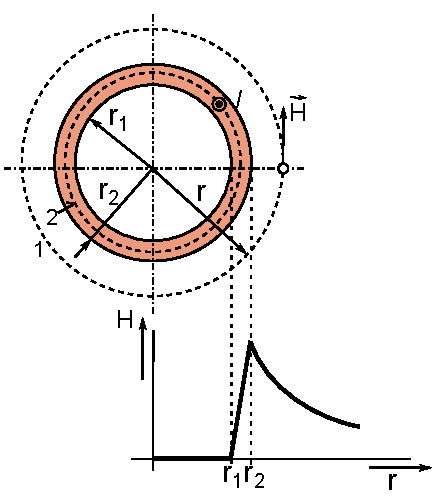
\includegraphics[width=0.8\linewidth]{teo_fig065.pdf}
      \captionof{figure}{K příkladu stanovení intenzity magnetického pole dlouhého dutého válcového 
                vodiče protékaného proudem}
      \label{teo:fig065}
    \par}
    
    Vodič s rovnoměrně rozloženým proudem podle obr. \ref{teo:fig065} je rotačně souměrný podle své
    osy a tedy i jeho magnetické pole je souměrné. Silové čáry jsou soustředné kružnice, vektor
    $\vr{H}$, jenž má směr tečny ke kružnici, je po celé délce kružnice stejně velký. Lze tedy
    snadno použít integrálního tvaru 1. MR (\textbf{zákon celkového proudu})
    
    Pro body ležící vně vodiče obepíná kruhová integrační dráha (vedená po silové čáře 1) celý
    proud vodiče $I$ a platí
    \begin{equation}\label{TEMP:eq_1MR_duty_valec}
      \oint_{\mathcal{C}}\vr{H}d\vr{l} = H\cdot 2\pi r = I
    \end{equation}
    takže intenzita pole je
    \begin{equation}\label{TEMP:eq_H_duty_valec}
      H = \frac{I}{2\pi r}
    \end{equation}
    
    Ve stěně dutého magnetického vodiče jsou silové čáry rovněž kružnice, neboť magnetické pole
    je i zde souměrné. Tyto siločáry však obepínají jen část proudu $I'$ vodiče pro oběh siločáry
    2 platí
    \begin{equation}\label{TEMP:eq_1MR_uvnitr_valce}
      \oint_{\mathcal{C}}\vr{H}d\vr{l} = H\cdot 2\pi r = I' = \pi(r^2-r_1^2)J
    \end{equation}
    kde $J$ je hustota proudu ve vodiči
    \begin{equation}\label{TEMP:eq_J_duty_valec}
      J = \frac{I}{S}= \frac{I}{\pi(r_2^2-r_1^2)}
    \end{equation}
    Ve stěně vodiče je tedy intenzita pole
    \begin{equation}\label{TEMP:eq_H_uvnitr_valce}
      H = \frac{I}{2\pi r}\frac{r^2-r_1^2}{r_2^2-r_1^2}
    \end{equation}
    V dutině vodiče je intenzita rovna nule. Vzhledem k souměrnosti pole by i zde muselo platit
    $\oint_{\mathcal{C}}\vr{H}d\vr{l} = H\cdot 2\pi r$. Protože dráha s poloměrem $r<r_1$ neobepíná
    žádný proud, je $\oint_{\mathcal{C}}\vr{H}d\vr{l} = 0$ a tedy musí byt $H = 0$.
  \end{example}    
\end{mdframed}  
      %------------------------------------------------------------------

      % --------example: $H=f(r)$ souosého kabelu -----------------------
      % \label{TEO:exam013}
      % !TeX spellcheck = cs_CZ
\begin{example}\label{TEMP:ex_koax_H}
  Stanovte intenzitu magnetického pole dlouhého přímého souosého kabelu podle obr.
  \ref{TEMP:fig_exam_koax}. Středním vodičem (\emph{žílou}) prochází proud $I$ a týž proud 
  opačného smyslu prochází vnějším vodičem (\emph{pláštěm}). Proudy jsou rovnoměrně rozloženy po 
  průřezech vodičů. Nakreslete graf průběhu $H = f(r)$ \cite[s.~92]{Dufek1970},
  \cite[s.~195]{Kotlan1999}.
  
  {\centering
   \begin{tabular}{cc}
     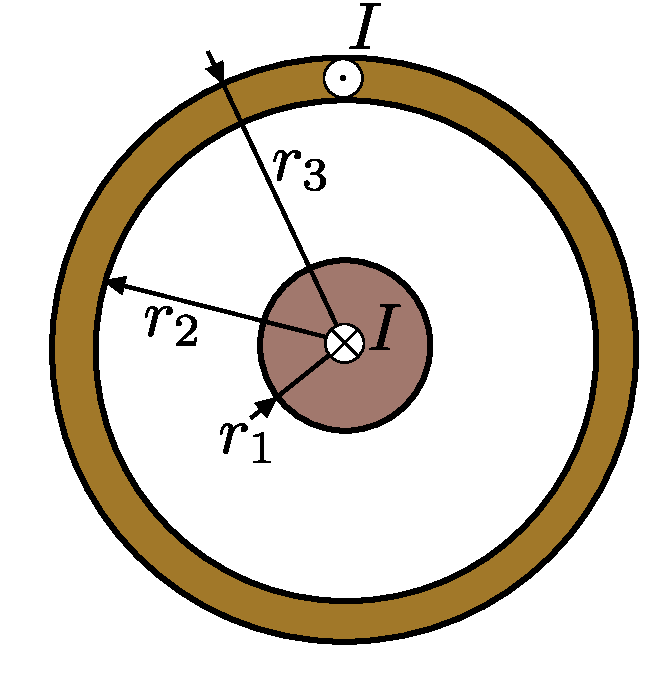
\includegraphics[width=0.4\linewidth]{vypocet_H_sousy_kabel.pdf}   &
     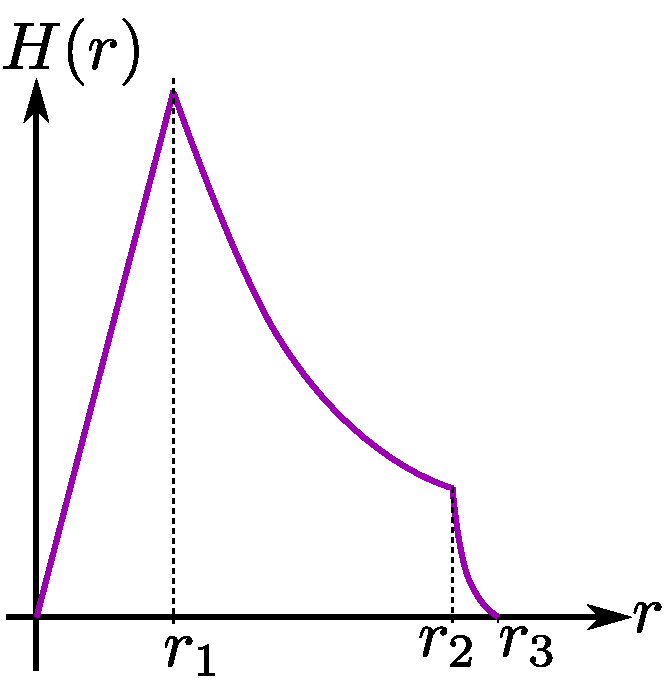
\includegraphics[width=0.4\linewidth]{koax_H_prubeh.pdf}
  \end{tabular}
  \captionsetup{type=figure}
  \captionof{figure}{K příkladu stanovení intenzity magnetického pole dlouhého souosého kabelu 
             protékaného proudem: a) náčrt; b) $H=f(r)$}
  \label{TEMP:fig_exam_koax}
  \par}
  
  \textbf{Řešení}: \newline Rovnici \ref{TEMP:eq_1MR_v_hom_p} aplikujeme na jednotlivé intervaly 
  osově souměrného stacionárního magnetického pole, přičemž se prakticky jedná o superpozici dvou
  polí. V oblasti $r<r_2$ se uplatňuje pouze pole vnitřního válcového vodiče (žíly), pro $r>r_2$ 
  přistupuje souosé pole vnějšího trubkového vodiče.
  \begin{itemize}
    \item Pro oblast $r<r_1$ je vzhledem k 
          \begin{align*}
              % \nonumber to remove numbering (before each equation)
              dI   &= \vr{J}d\vr{S} \\
              I(r) &= \int_S dI = \int_S \vr{J}d\vr{S} = \int_S J\cos\beta dS \\
                   &= \left|\begin{array}{cc}
                               \beta = 0 & H = \text{konst} \\
                             S = \pi r^2 & dS = 2\pi rdr \\
                            \end{array}
                      \right| = J\int_0^r 2\pi rdr = J\pi r^2
          \end{align*}
          hledané řešení 1. MR dáno 
          $$\oint_\mathcal{C}\vr{H}d\vr{l} = H_1 2\pi r = I(r) = J\pi r^2$$ kde celková proudová
          hustota je  $$J = \frac{I}{\pi r_1^2}$$ a tedy $$H_1 = \frac{I}{2\pi r_1^2}\cdot r$$
          
    \item Pro oblast $r_2>r>r_1$ řešíme v podstatě pole vně osamoceného válcového vodiče
          $I(r)$ a tedy $$H_2 = \frac{I}{2\pi r}$$
    \item Pro $r>r_3$ je magnetické pole vytvářeno celým proudem žíly $I$ a příslušnou částí
          proudu pláště $J\pi(r^2 - r_2^2)$, kde proudová hustota $$J =
          \frac{I}{\pi(r_3^2-r_2^2)}$$ má opačnou orientaci oproti proudové hustotě žíly. Pak 
          \begin{align*}
            I(r)                           &= I - I\frac{r^2-r_2^2}{r_3^2-r_2^2} \\
            \oint_\mathcal{C}\vr{H}d\vr{l} &= H_32\pi r = I(r)                   \\          
            H_3                            &= \frac{I}{2\pi r}\left(1 - 
            \frac{r^2 - r_2^2}{r_3^2 - r_2^2}\right) 
          \end{align*}
          Stejný výsledek dostaneme superpozicí opačně orientovaných polí $$H_3 = H'_3 - H''_3 =
          \frac{I}{2\pi r} - \frac{I}{2\pi r}\left(\frac{r^2 - r_2^2}{r_3^2 - r_2^2}\right)$$. 
  \end{itemize}
  Průběh $H(r)$ je na obr. \ref{TEMP:fig_exam_koax}.
\end{example}
  
      %------------------------------------------------------------------

    % -----------Magnetické pole elektrického proudu v diferenciálním tvaru-----------------------
    \subsection{Magnetické pole elektrického proudu v diferenciálním tvaru}
      Nechť je opět magnetické pole vyvoláno konstantním el. proudem $I = \text{konst}$. Jak
      vyplývá z předchozí kapitoly, základním vztahem pro toto pole je \emph{Ampérův zákon}
      $$\oint_{\mathcal{c}}\vec{H_c}\dd{\vec{l}} = I$$  Zvolme za integrační dráhu $c$ obvod malé plošky
      $\Delta S$, jíž prochází proud $\Delta I = J_n \Delta S$, kde $J_n$ je průmět vektoru hustoty
      proudu do směru normály plošky $\Delta S$ (předpokládáme, že ploška $\Delta S$ je dostatečně
      malá, aby se dalo počítat s konstantní hustotou proudu v celém jejím rozsahu)
      \cite[s.~13]{Trnka1972}. Pro zvolený případ platí
      
      \begin{equation}\label{TEMP:eq_amp_z1}
        \oint_{\mathcal{c}}\vec{H_c}\dd{\vec{l}}  =
          J_n \Delta S \rightarrow \frac{1}{\Delta S}\oint_{\mathcal{c}}\vec{H_c}\dd{\vec{l}} = J_n
      \end{equation} 
      
      Pro $\Delta S \rightarrow 0$ zavedeme označení 
      \begin{equation}\label{TEMP:eq_amp_z2}
        \rot{H}  = \frac{1}{\Delta S}\oint_{\mathcal{c}}\vec{H_c}\dd{\vec{l}}  = J_n
      \end{equation}
      
      Rovnice \ref{TEMP:eq_amp_z2} říká, že \emph{rotace vektoru} $\vec{H}$, ($\rot{H}$), jehož
      průmět do určitého směru je roven průmětu vektoru hustoty proudu do tohoto směřu. Z uvedených
      vztahu je patrný fyzikální význam rotace vektoru $\vec{H}$. Je to vektor, jehož velikost je
      rovna oběhovému magnetickému napětí po dráze v rovině kolmé k vektoru hustoty proudu,
      vztaženém k ploše obepínané oběhovou drahou (v nehomogenní poli to platí pro případ, že se
      plocha dráhy blíží k nule).
      
      Při použití pravoúhlé soustavy kartézských souřadnic \(x\), \(y\) a $z$ jsou průměty vektoru
      $\rot{H}$ do jednotlivých os
      \begin{equation}\label{TEMP:eq_amp_z3}
        \textsf{rot}_x\vec{H} = J_x,   \quad
        \textsf{rot}_y\vec{H} = J_y,   \quad
        \textsf{rot}_z\vec{H} = J_z    
      \end{equation}      
      Průmět $\textsf{rot}_x\vec{H}$ je dán oběhovým magnetickým napětím po obvodu plošky
      \(\dd{y}\dd{z}\) a platí
      \begin{align*}
        \textsf{rot}_x\vec{H} 
        &=\frac{1}{\dd{y}\dd{z}}\oint_{\mathcal{c}}\vec{H_c}\dd{\vec{l}} =               \nonumber\\
        &=\frac{1}{\dd{y}\dd{z}}\cdot\Biggl[\Biggr.\left[H_y\dd{y} 
         +\left(H_z + \pder{Hz}{y}\dd{y}\right)\dd{z}\right]                             \nonumber\\     
        &-\left[\left(H_y-\pder{H_y}{z}\dd{z}\right)\dd{y}-H_z\dd{z}\right]\Biggl.\Biggr]\nonumber\\
        &=\pder{H_z}{y}\dd{y}\dd{z} - \pder{H_y}{z}\dd{y}\dd{z}                          \nonumber\\    
        &=\pder{H_z}{y} - \pder{H_y}{z} = J_z
      \end{align*}       
      
      \luagraphic[0.8]{teo_fig062.pdf}{K odvození pojmu \(\textsf{rot}_z\vec{H}\)}{teo:fig062}
         
      tedy dostáváme
      \begin{subequations}
        \begin{align}\label{TEMP:eq_amp_z5}
          \textsf{rot}_x\vec{H} &= \pder{H_z}{y} - \pder{H_y}{z} = J_x       \\
          \textsf{rot}_y\vec{H} &= \pder{H_x}{z} - \pder{H_z}{x} = J_y       \\
          \textsf{rot}_z\vec{H} &= \pder{H_y}{x} - \pder{H_x}{y} = J_z            
        \end{align}    
    \end{subequations}    
      Pro \emph{pravoúhlé souřadnice} $x, y, z$ můžeme tedy vztah $\rot{H} = \vec{J}$ rozepsat na
      tvar
      \begin{align*}
        \textsf{rot}\vec{H} 
          &= \vec{i}\,\textsf{rot}_x\vec{H} + 
             \vec{j}\,\textsf{rot}_y\vec{H} +
             \vec{k}\,\textsf{rot}_z\vec{H}                                    \\
          &= \vec{i}\left(\pder{H_z}{y} - \pder{H_y}{z}\right) +               \\
          &+ \vec{j}\left(\pder{H_x}{z} - \pder{H_z}{x}\right) +               \\
          &+ \vec{k}\left(\pder{H_y}{x} - \pder{H_x}{y}\right)                 \\  
          &= \vec{i}\,J_x + \vec{j}\,J_y + \vec{k}\,J_z = \vec{J}.
      \end{align*}          
      
      Rotaci vektoru $\rot{H}$ můžeme též symbolicky vyjádřit vektorovým součinem Hamiltonova
      operátoru a vektoru $\vec{H}$
      \begin{align*}
        \rot{H} &= \nabla\times\vec{H}                                                      \\                                           
                &= \left(\vec{i}\,\pder{ }{x} + 
                   \vec{j}\,\pder{ }{y} + \vec{k}\,\pder{ }{z}\right)                       \\
                & \times(\vec{i}\,H_x + \vec{j}\,H_y + \vec{k}\,H_z)
      \end{align*}
      nebo také determinantu
      \begin{equation}\label{TEMP:eq_amp_z8}
        \rot{H} = \begin{vmatrix}
                    \vec{i}       & \vec{j}      & \vec{k}      \\
                    \pder{ }{x}  & \pder{ }{y} & \pder{ }{z} \\ 
                    H_x          & H_y         & H_z         \\
                  \end{vmatrix}      
      \end{equation}  
      \emph{cylindrických souřadnic} $r$, $\varphi$, $z$:
      \begin{align}\label{TEMP:eq_amp_z9}
        \textsf{rot}_r\vec{H}       
          &= \frac{1}{r}\pder{H_z}{\varphi} - \pder{H_\varphi}{z} = J_r           \nonumber \\ 
        \textsf{rot}_\varphi\vec{H} 
          &= \pder{H_r}{z} - \pder{H_z}{r}                        = J_\varphi     \nonumber \\
        \textsf{rot}_z\vec{H}       
          &= \frac{1}{r}\left[\pder{ }{r}
             \left(rH_\varphi\right)-\pder{H_r}{\varphi}\right]   = J_z
      \end{align} 
      \emph{sférických souřadnic} $r$, $\varphi$, $\vartheta$ 
      \begin{align}\label{TEMP:eq_amp_z10}
        \textsf{rot}_r\vec{H}        
           &= \frac{1}{r\sin\vartheta}\left[\pder{ }{\vartheta}(H_\varphi\sin\vartheta) - 
              \pder{H_\vartheta}{\varphi}\right]                     = J_r           \nonumber \\ 
        \textsf{rot}_\varphi\vec{H}   
           &= \frac{1}{r}\left[\pder{ }{r}(rH_\vartheta) - 
              \pder{H_r}{\vartheta}\right]                           = J_\varphi     \nonumber \\
        \textsf{rot}_\vartheta\vec{H} 
           &= \frac{1}{r\sin\vartheta}\left[\pder{H_r}{\varphi} -
              \pder{ }{r}\left(rH_\varphi\sin\vartheta\right)\right] = J_\vartheta    
    \end{align} 
      Podobně jako v elektrickém poli vyjadřujeme vztah $\oint\vec{D}\dd{\vec{S}} = Q$ vztahem 
      $\diver{D}
      = \rho$, tak i v magnetickém poli vyjadřujeme vztah $\oint\vec{B}\dd{\vec{S}} = 0$ vztahem
      $\diver{D} = 0$, nebo též v kartézských souřadnicích \(x\), \(y\) a $z$ jako $$\diver{D} =
      \nabla\cdot\vec{B} = \pder{B_x}{x} + \pder{B_y}{y} + \pder{B_z}{z} = 0$$
                     
    % ----------------Rovnice pro magnetický potenciál -------------------------------------------
    \subsection{Rovnice pro magnetický potenciál}
      V regulárních bodech lineárního homogenního izotropního magnetika platí pro $\varphi_m$
      \textbf{Laplaceova rovnice}
      \begin{equation}\label{TEMP:eq_varphi_m_laplace}
        \Delta\varphi_m = 0
      \end{equation}      
      Důkaz plyne z rovnice $\diver{B} = 0$ a rovnice $\vec{B} = \mu\vec{H}$: $$\diver{B} =
      \textsf{div}\mu\vec{H} = \textsf{div}\mu(-\textsf{grad}\varphi_m).$$ Pro $\mu = \text{konst}$
      dostáváme $\textsf{div}\textsf{grad}\varphi_m = 0$, což je rovnice
      \ref{TEMP:eq_varphi_m_laplace}.
      
      Na rozhraní mezi dvěma magneticky různými prostředími neplatí Maxwellovy rovnice v
      diferenciálním tvaru a tedy ani Laplaceova rovnice \ref{TEMP:eq_varphi_m_laplace}. Podmínky 
      pro $\vec{H}$ a $\vec{B}$ na rozhraní vyjádříme pomocí skalárního magnetického potenciálu
       \begin{align}\label{TEMP:eq_mag_U_rozhrani}
         \varphi_{m1}                 &= \varphi_{m2} \\
         \mu_1\pder{\varphi_{m1}}{n}  &= \mu_2\pder{\varphi_{m2}}{n} 
       \end{align}
      kde $\pder{}{n}$ jsou derivace ve směru normály k rozhraní. 
    
    \subsubsection{Vektorový magnetický potenciál}
      V elektrostatice jsme pro usnadnění mnohých problémů zavedli skalární elektrický potenciál -
      lze jej zavést vždy, neboť elektrostatické pole je vždy potenciální. Magnetické pole je však
      obecně vírové. Lze jej popsat skalárním potenciálem jen ve speciálních případech, tj.
      jestliže je polem potenciálním. Obecně je však zavedení skalárního potenciálu nepřípustné.
      Lze i pak zavést nějakou veličinu (analogickou skalárnímu potenciálu), s níž by se pracovalo
      snáze, než přímo s vektory pole?
      
      Dříve než definujeme vektorový magnetický potenciál, zopakujme zavedení skalárního potenciálu
      v elektrostatice. Vyjdeme z 2. MR a z rovnice známé z vektorové analýzy: $$\rot{E} = 0 \quad
      \text{a} \quad \textsf{rot}\,\textsf{grad}\varphi_m = 0.$$
      
      V magnetickém poli vyjdeme ze 4. MR a z jiné identity pro vektorovou funkci $\vec{A}$, známe z
      vektorové analýzy: $$\diver{B} = 0 \quad \text{a} \quad \textsf{div}\textsf{rot}\vec{A} =
      0$$ odtud
        \begin{equation}\label{TEMP:eq_B_rotA}
          \vec{B} = \rot{A}.
        \end{equation}       
               
%} % tikzset
%~~~~~~~~~~~~~~~~~~~~~~~~~~~~~~~~~~~~~~~~~~~~~~~~~~~~~~~~~~~~~~~~~~~~~~~~~~~~~~~~~~~~~~~~~~~~~~~~~~
%========== Kapitola: Základní zákony elektromagnetismu ============================================
  % !TeX program = lualatex
% !TeX root = luaking.tex
% !TeX encoding = UTF-8
% !TeX spellcheck = cs_CZ
%---------------------------------------------------------------------------------------------------
% file magn1ch01.tex
\graphicspath{{../src/TEO/img/}}
%---------------------------------------------------------------------------------------------------
%====================Kapitola: Základní zákony elektromagnetismu====================================
\setchaptertoc
\chapter{Základní zákony elektromagnetismu}\label{teo:IchapII}
  V této teoreticky změřené kapitole budou shrnuty základní fyzikální zákony, kterými se řídí
  elektromagnetické jevy a jejichž znalost bude nezbytná při studiu následujících praktičtěji
  zaměřených kapitol. Mezi nejdůležitější patří zákon elektromagnetické indukce. Velký praktický
  význam má jeho zobecnění i pro případy nejsložitější, jakými jsou \emph{nelineární} a navíc
  \emph{parametrické} magnetické obvody. Důležitým pojmem je \emph{spřažený} magnetický tok cívky.
  Pro hlubší pochopení všech zákonitostí bude vhodné upozornit na \emph{topologické vlastnosti}
  elektromagnetického pole. Ukazuje se totiž, že topologický přístup je velice užitečným a silným
  nástrojem, který významně usnadňuje pochopení \wikiMaxwellEq se všemi jejich důsledky
  \cite[s.~6]{Patocka4}. Topologii elektromagnetického pole je proto věnována celá kapitola
  \ref{teo:IchapIII}
  
  \section{Zákon elektromagnetické indukce}\label{teo:IchapIIsecI}
    Základní veličinou pro popis magnetických polí a jejich účinků je \emph{vektor magnetické
    indukce} \(\vec{B}\). Dle soustavy SI je jednotkou magnetické indukce \emph{tesla} \([T]\) a
    projevuje se silovými účinky na vodiče protékané proudy a indukováním napětí při jeho změně.

    Je proto dobře měřitelný. První rovnice (Ampérův zákon) ze souboru Maxwellových rovnic určuje
    rovnost oběhového integrálu magnetické indukce po uzavřené křivce proudům protékaných vodiči,
    jež jsou touto křivkou uzavřeny.
    \begin{equation}\label{TEO:eq101}
      \oint_l \vec{B} \cdot \vec{\dd{l}} = \sum I
    \end{equation}
    
    \luagraphic[0.4]{teo_fig034.pdf}{Elektrický proud ve vodiči způsobuje vznik magnetické pole v 
      jeho okolí.}{teo:fig034}

    Obrázek \ref{teo:fig034} ilustruje fakt, že elektrické proudy jsou vždy obklopeny 
    magnetickými poli. Tato pole se dají zesílit cívkou s magnetickým jádrem. Na tomto jevu je 
    založen jeden z elementárních principů elektrotechniky.    
       
    \begin{mdframed}[style=mdnote]
      Jaký je vztah jednotky magnetické indukce k ostatním základním jednotkám soustavy \textbf{SI}? 
      \begin{align*}
        \SI{1}{\tesla}
          &= 1\frac{V\cdot s}{m^2} = 1\frac{N}{A\cdot m} = 1\frac{Wb}{m^2}          \\
          &= 1\frac{kg}{C\cdot s} = 1\frac{kg}{A\cdot s^2} = 1\frac{N\cdot s}{C \cdot m}
      \end{align*}
    \end{mdframed}
    
    Při odvozování matematického modelu transformátoru se obvykle vychází ze zákona 
    \textbf{elektromagnetické indukce}, který říká, že \emph{časová změna magnetického pole vytvoří 
    vírové pole elektrické}:
    \begin{equation}\label{es:eq_ind_z}
      \oint_l \vec{E} \cdot \dd{\vec{l}} = - \der{\Psi}{t}
    \end{equation}
     
    Základní laboratorní experimenty, vedoucí k odhalení existence tohoto zákona, uskutečnil 
    \textsc{M. Faraday}\footnote{Michael Faraday (1791 - 1867), samouk, zakladatel klasické 
    elektrodynamiky, vynikající experimentátor: Zavedl pojem fyzikálního prostorového pole pomocí 
    siločár, tzv. ''trubic''} v roce 1831. Matematickou formulaci \emph{indukčního zákona} v podobě 
    rovnice
    \begin{equation}\label{TEO:eq102}
      u(t) = - \frac{d\Psi(t)}{\dd{t}}
    \end{equation} 
    stanovil již on sám, postupně význam zákona formálně upřesňovali další badatelé např. \textsc{F.
    E. Neumann}\footnote{Franz Ernst Neumann (1798 - 1895), teoretický fyzik, matematik, mineralog.
    Definoval pojem magnetický vektorový potenciál, formuloval Neumannův vzorec pro vzájemnou
    indukčnost dvou smyček. Učitel G. R. Kirchhoffa.} kolem roku 1845. Konečné znění Maxwellovy
    teorie včetně formulace indukčního zákona do podoby II. Maxwellovy rovnice budoval \textsc{J. C.
    Maxwell}\footnote{James Clark Maxwell (1831 - 1879), teoretický fyzik, působil na Trinity
    College university v Cambridge, na King's College v Londýně, posléze první ředitel Cavendishovy
    laboratoře na univerzitě v Cambridge. Původně se zabýval teoretickou mechanikou a kinetickou
    teorií plynů. Soustavu čtyř Maxwellových rovnic odvodil především na základě
    mechanicko-elektrických analogií.} velmi pozvolna, v období 1855 až 1873. Z historického pohledu
    je zajímavé a důležité, že přesné \emph{kvantitativní} experimenty s elektromagnetickou indukcí
    byly v té době uskutečnitelné pouze pomocí \wikiGalvanometer. Lze odhadnout, že nebýt tohoto
    přístroje, přesná matematická formulace indukčního zákona by se pravděpodobně opozdila o několik
    let. Kupodivu, z psychologického hlediska je i v současnosti velmi vhodné vysvětlit princip
    indukčního zákona pomocí historických pokusů s balistickým galvanometrem.
    
    \subsection{Pokusy s balistickým galvanometrem}
      Jako každý elektromagnetický měnič energie (tj. motor), obsahuje i \emph{magnetoelektrické
      měřicí} ústrojí galvanometru dva akumulátory energie: moment setrvačnosti \(J\) otoč\-né 
      části a indukčnost cívky \(L\). Jedná se tedy o kmitavou soustavu 2. řádu. Každou takovou 
      soustavu lze kriticky, případně nadkriticky tlumit - především zařazením tlumicího odporu 
      vhodné velikosti do série s měřicím systémem (tlumení vlivem mechanického tření je úmyslně 
      konstrukčně potlačeno na zanedbatelnou úroveň). Balistický galvanometr je cíleně konstruován 
      s velkým momentem setrvačnosti \(J\) a s malou tuhostí \(k_d\) direkčních pružin, aby měl 
      dlouhou dobu kmitu \(T_G = 2\pi\sqrt{J/k_d}\) několik sekund. Proteče-li galvanometrem krátký 
      proudoý impuls \(i(t)\) o celkové délce \(t_i\) podle obr. \ref{teo:fig036}, pak lze snadno 
      dokázat, že za předpokladu \(t_i\ll T_G\) je první maximální výchylka \(\alpha_{max}\) 
      tlumeného pohybu ukazatele přímo úměrná celkovému náboji \(Q\) proudového impulsu podle 
      rovnice 
      \begin{equation}\label{TEO:eq103}
        \alpha_{max} = k_b Q = k_b\int_0^{t_i} i(t)\dd{t},
      \end{equation}
      kde \(k_b\) je \emph{balistická konstanta} použitého galvanometru. Balistický galvanometr tedy
      pracuje jako \emph{integrátor} proudu v přesném matematickém smyslu. 
      
      \luagraphic[1]{teo_fig036.pdf}{Příklad krátkého proudového impulsu prošlého balistickým 
        galvanometrem.}{teo:fig036}
  
      Uvažujme experiment uspořádaný podle obr. \ref{teo:fig037}. V uzavřeném obvodu
      galvanometru se nachází celkový odpor \(R\) a tuhá samonosná cívka v podobě kruhového závitu,
      připojená na dlouhé ohebné zkroucené přívody. Husté zkroucení zajišťuje, že do samotných
      přívodů se nemůže indukovat žádné napětí, pohybuje-li se cívka v magnetickém poli 
      permanentního magnetu. Při rychlém přesunu z polohy \emph{1} do vzdálené polohy \(\infty\) 
      klesne v cívce magnetický tok na nulu, časová změna toku zapříčiní vznik indukovaného napětí, 
      napětí protlačí obvodem proudový impuls odpovídající přibližně obr. \ref{teo:fig036}.
      
      \luagraphic[0.8]{teo_fig037.jpg}{Uspořádání experimentálního pracoviště s balistickým 
        galvanometrem}{teo:fig037}
      
      Za předpokladu kritického nebo nadkritického tlumení má odpor \(R\) relativně velkou hodnotu. 
      Proto lze s dobrou přesností zanedbat vnitřní indukčnost měřicího systému galvanoměru a 
      uvažovat, že celé napětí \(u(t)\), indukované v cívce při jejím pohybu, spočine pouze na 
      odporu. V uzavřeném okruhu o celkovém odporu \(R\) pak platí Ohmův zákon ve tvaru
      \begin{equation}\label{TEO:eq104}
        i(t)=\frac{u(t)}{R}.
      \end{equation}    
      Dosadíme-li rovnici \ref{TEO:eq104} do \ref{TEO:eq103}, po úpravě získáme vztah
      \begin{equation}\label{TEO:eq105}
       \int_0^{t_i}u(t)\dd{t}=\frac{\alpha_{max}R}{k_b}.
      \end{equation}     
      Experimentálně je možno dospět ke dvěma stěžejním poznatkům:
      \begin{itemize}
        \item Při přesunu cívky z polohy \emph{1} do polohy \(\infty\) nezávisí výchylka
              \(\alpha_{max}\) na \emph{rychlosti pohybu}. (Za předpokladu \(t_i\ll T_G\), což je
              omezení dané nedokonalostí přístroje a nijak nesouvisí se zkoumaným jevem.)
        \item Při přesunu cívky z polohy \emph{1} do polohy \(\infty\) zůstává součin
              (\(\alpha_{max}\times R\)) stále \emph{konstantní}, měníme-li úmyslně velikost odporu
              \(R\). To jest: při k-násobném zvýšení odporu klesne výchylka k-krát a naopak. 
      \end{itemize}
  
      V poloze „1“ prochází plochou cívky magnetický tok \(\Psi\). V poloze „\(\infty\)“ je zřejmě
      magnetický tok cívky nulový, tedy \(\Psi_\infty = 0\). S ohledem na rovnici
      (\ref{TEO:eq105}) lze pak oba experimentální poznatky interpretovat jediným možným
      způsobem:
       \begin{equation}\label{TEO:eq106}
       \int_0^{t_i}u(t)\dd{t}=\text{konst}=\Psi-\Psi_\infty=\Psi.
      \end{equation}    

      Experiment lze opakovat s cívkami libovolných rozměrů, tvarů i počtů závitů. Výsledky budou
      kvalitativně stejné. Veličina \(\Psi\) se nazývá \emph{spřažený magnetický tok cívky}. Je to 
      míra interakce cívky s magnetickým polem, které spojitě prostupuje celou plochou cívky. 
      Rovnici (\ref{TEO:eq106}) lze vyjádřit slovně: Spřažený magnetický tok cívky je úměrný 
      časovému integrálu svorkového napětí na zkoumané cívce. Je určitě výhodné zvolit jedničku 
      jako konstantu úměrnosti mezi tokem \(\Psi\) a integrálem napětí. \emph{Pak bude velikost 
      spřaženého toku přímo rovna integrálu napětí}. Určitý integrál v rovnici 
      (\ref{TEO:eq106}) lze nahradit integrálem neurčitým, pak je ale nutno přidat obecnou 
      počáteční integrační konstantu \(\Psi_0\)
      v newtonovském smyslu. Získáme tak zákon elektromagnetické indukce (indukční zákon) v
      integrálním tvaru
      \begin{equation}\label{TEO:eq107}
       \Psi(t) = \Psi_0 + \int u(t)\dd{t} \quad [Wb;\, V,\; s].
      \end{equation}   
    
    Z rovnice (\ref{TEO:eq107}) plyne, že jednotka magnetického toku Weber\footnote{Wilhelm Eduard
    Weber (1804-1891), teoretický fyzik, působil na univerzitách v Gottingenu a v Lipsku. Zakladatel
    předrelativistické elektrodynamiky. Určil totiž silu mezi náboji v závislosti nejen na
    vzdálenosti, ale i na rychlosti a zrychlení, jeho teorie je ale platná pouze pro \(v \ll c\).
    Blízký spolupracovník Gausse.} má rozměr \([Vs]\), Budeme-li obě strany rovnice derivovat podle
    času, rovnost tím neporušíme. Získáme tak ryze matematickou cestou indukční zákon v
    diferenciálním tvaru
    \begin{equation}\label{TEO:eq108}
     u(t) = \frac{d\Psi(t)}{\dd{t}}, \quad \text{resp.} \quad  u(t) = -\frac{d\Psi(t)}{\dd{t}}.
    \end{equation}   
    Obě rovnice (\ref{TEO:eq108}a), (\ref{TEO:eq108}b) se liší znaménkem \(+\) nebo \(-\) na pravé
    straně. Volba znaménka souvisí s domluvou, který režim cívky považujeme za základní: zda režim
    \emph{spotřebičový} podle rovnice (\ref{TEO:eq108}a), nebo režim \emph{zdrojový} podle rovnice
    (\ref{TEO:eq108}b). Oba režimy jakéhokoli dvojpólu jsou totiž jednoznačně definovány vzájemnou
    orientací napětí a proudu podle obr. \ref{teo:fig039}. Odpor nemůže nikdy pracovat jako zdroj,
    proto slouží jako „normál“ definující \emph{spotřebičovou} orientaci svorkových veličin. Oba
    režimy cívky se liší níže popsaným způsobem.

    \begin{figure}[ht!]
      \centering  
      \subcaptionbox{Odpor je vždy spotřebičem     \label{teo:fig039a}}
        {\luafigure[0.4]{teo_fig039a.pdf}}                    
      \subcaptionbox{Cívka ve spotřebičovém režimu \label{teo:fig039b}}
        {\luafigure[0.4]{teo_fig039b.pdf}}         \\               
      \subcaptionbox{Cívka ve zdrojovém režimu     \label{teo:fig039c}}
        {\luafigure[0.4]{teo_fig039c.pdf}}
      \caption{Vzájemná orientace okamžité hodnoty proudu a napětí ve spotřebičovém a zdrojovém 
               režimu.} 
      \label{teo:fig039}
    \end{figure}
        
    \textbf{Spotřebičový režim:}
    \begin{itemize}[noitemsep]
      \item Orientace svorkového napětí \(u(t)\) je vůči proudu \(i(t)\) souhlasná. Platí rovnice
            (\ref{TEO:eq108}a).
      \item Cívka je připojena na zdroj napětí\(u(t)\), odebírá z něj proud \(i(t)\), tedy odebírá
            ze zdroje elektrickou energii a chová se jako spotřebič. Tuto energii přeměňuje na
            energii magnetického pole.
      \item Mezi směrem proudu a směrem toku platí \emph{pravidlo pravé ruky}, PPR.           
    \end{itemize}
    
    \textbf{Zdrojový režim:}
    \begin{itemize}[noitemsep]
      \item Orientace svorkového napětí u(t) je vůči proudu i(t) nesouhlasná. Platí rovnice
            (\ref{TEO:eq108}b).
      \item Cívka je vložena do proměnného magnetického pole \(B(t)\), na jejích svorkách vzniká
            indukované napětí \(u(t)\) (zastaralý výraz: „elektromotorická síla“). Z cívky se stal
            zdroj elektrického napětí u(t), tj. generátor. Připojíme-li na svorky odporovou zátěž,
            začne do ní generátor dodávat elektrickou energii.\footnote{Faraday s Maxwellem se znali
            osobně a po dohodě pokládali zdrojový režim cívky za základní, tedy pracovali s rovnicí
            (\ref{TEO:eq108}b). Maxwell navíc pracoval s pojmem „electromotive force \(P\)‘, který
            svým významem přesně odpovídal dnešní „intenzitě elektrického pole. Postupem času byl
            doslovně přeloženému výrazu „elektromotorická síla“ nešťastně přiřazen v české i
            zahraniční literatuře význam „napětí“, což ještě více zvýšilo zmatek. Proto je rozumné
            výraz „elektromotorická síla“ vůbec nepoužívat.}
    \end{itemize}

    \luagraphic[1]{teo_fig038.jpg}{Princip transformátoru. Primární cívka pracuje ve
    spotřebičovém režimu (PPR), sekundární cívka ve zdrojovém režimu (PLR)}{teo:fig038}

    Z uvedených skutečností lze učinit následující závěr. Volba znaménka v rovnicích
    (\ref{TEO:eq108}a, b) je věcí dohody, ale pouze v tom smyslu, zda zvolíme za základní režim
    spotřebičový či zdrojový\footnote{Ojediněle se v literatuře, např. v [5], vyskytne názor, že
    znaménko v rovnicích (\ref{TEO:eq108}a, b) je určeno tím, zda je cívka navinuta pravotočivě nebo
    levotočivé. To je chybné tvrzení. Pravotočivost či levotočivost cívky naprosto nijak nesouvisí
    se schopnosti cívky pracovat ve zdrojovém nebo spotřebičovém režimu.}. Například při analýze
    měničů ve výkonové elektronice je ustáleným zvykem zvolit označení proudu a napětí na
    indukčnosti podle obr. \ref{teo:fig039b}. Bez ohledu na tuto volbu musíme v konkrétní situaci
    vždy pečlivě rozlišovat, ve kterém režimu se cívka skutečně nachází. Příklad: primární cívka
    transformátoru se nachází vždy ve spotřebičovém režimu, sekundární cívka vždy ve zdrojovém
    režimu. Se zdrojovým či spotřebičovým režimem úzce souvisí \emph{Lenzův
    princip}\footnote{Heinrich Lenz (1804-1865), estonský fyzik, působil na univerzitě v Petrohradu.
    Princip po něm pojmenovaný objevil r. 1833.}. Jedná se o zvláštní případ obecnějšího přírodního
    principu, vyjádřitelného jako „zákon akce a reakce“. V elektromagnetismu má zákon následující
    tvar:

    Lenzův princip: Proud indukovaný v uzavřené vodivé smyčce vyvolá magnetické pole, které působí
    vždy proti původnímu budicímu poli, díky němuž indukovaný proud vznikl.

    Všimněme si, že zmíněná „uzavřená vodivá smyčka“ se nachází \emph{zdrojovém režimu}: je vložena
    do magnetického pole, indukuje se v ní napětí \(u(t)\), které protlačí vodivým obvodem proud
    \(i(t)\). Proud má ve \emph{zdrojovém režimu} takový směr, že působí proti budicímu magnetickému
    poli. Příkladem je již zmíněná sekundární cívka transformátoru podle Obr. /./-*/« nebo uzavřená
    smyčka vířivého proudu ve vnitřním prostoru transformátorového plechu podle Obr. 1.1-5.

    \luagraphic[1]{teo_fig040.jpg}{Vznik vířivého proudu uvnitř elektricky vodivého
    transformátorového plechu. Budicí cívka pracuje ve spotřebičovém režimu (PPR). Elementární
    smyčka vířivého proudu odpovídá sekundárnímu vinutí a pracuje ve zdrojovém režimu
    (PLR).}{teo:fig040}

    Integrací rovnice (\ref{TEO:eq108}a) lze zpětně dojít k integrálnímu tvaru
    (\ref{TEO:eq107}). Je nutno zdůraznit, že obě rovnice jsou naprosto rovnocenné, navzájem
    převoditelné, obě nesou stejné množství informace, žádná není důležitější než druhá. Je
    pravdou, že z psychologického pohledu je indukční zákon snáze pochopitelný v
    \emph{diferenciálním} tvaru (\ref{TEO:eq108}). Pro hluboké porozumění magnetickým jevům
    je však nezbytné uvědomit si především jeho \emph{integrální} podobu (\ref{TEO:eq107})
    se všemi matematickými důsledky:
    \begin{itemize}
      \item Spřažený tok je roven integrálu napětí. Zákon platí \emph{univerzálně}, bez ohledu na
            \emph{linearitu} či \emph{nelinearitu} magnetického obvodu. Rovnice
            (\ref{TEO:eq107}) totiž definuje funkční závislost \(\Psi=\Psi(u)\) mezi tokem a
            napětím, nikoli závislost \(\Psi=\Psi(i)\) mezi \emph{tokem a proudem}.  Případná
            nelinearita se totiž týká výlučně závislosti \(\Psi=\Psi(i)\), a tudíž nijak nenarušuje
            platnost rovnice (\ref{TEO:eq107}).
      \item Z předchozího bodu plyne, že v obecném \emph{nelineárním} případě není tok \(\Psi\)
            přímo úměrný proudu \(i\). Přímá úměra \(\Psi = Li\) totiž platí pouze ve zvláštním
            případě \emph{lineárního} magnetického obvodu.
      \item Rovnice (\ref{TEO:eq107}) platí ve spotřebičovém i generátorovém režimu cívky.
            Problém se znaménkem zůstává stejný jako u rovnic (\ref{TEO:eq108}).
      \item V uzavřené \emph{supravodivé} smyčce platí vždy \(u = 0\), i když jí teče konstantní
            ss. proud. Neurčitý integrál v rovnici (\ref{TEO:eq107}) má pak nulovou hodnotu
            \(\int0\dd{t}=0\), a zřejmě tedy platí \(\Psi(t)=\Psi_0\), kde \(\Psi_0\) je
            \emph{libovolná} počáteční integrační konstanta. Fyzikálně má konstanta význam
            počátečního toku, který je v cívce naintegrován z předchozích dějů. Případ
            \(\Psi_0\neq0\) odpovídá nabuzenému supravodivému magnetu, jehož tok \(\Psi(t)=\Psi_0
            = \text{konst.}\) se s časem nemění. Nabuzený supravodivý magnet se proto chová jako
            \emph{permanentní} magnet. Případ \(\Psi_0 = 0\) odpovídá magnetickému stínění pomocí
            \emph{závitu nakrátko}, např. tzv. Faradayova klec, nebo stínění koaxiálního kabelu
            podle obr. \ref{teo:fig041}. Každé oko \textbf{a-b-c-d} stínícího pláště
            tvoří „supravodivý“ závit nakrátko, v němž platí \(u = 0\), tedy \(\Psi=\int0\dd{t}=0\).
            Proto se do vnitřního prostoru ohraničeného pláštěm nemůže zvenčí dostat žádné
            \emph{střídavé} rušivé magnetické pole (jedině pole \emph{stejnosměrné} \(\Psi_{ss}\),
            ale to je neškodné, protože nezpůsobuje vznik rušivého napětí ve středním vodiči
            kabelu; derivace konstanty je totiž nulová: \(u(t)=\frac{d\Psi_{ss}}{\dd{t}}=0\)).
    \end{itemize}

    Na otázku „Proč je magnetický tok úměrný integrálu napětí?“ lze odpovědět pouze následujícím
    způsobem: „Protože je to jeden ze základních zákonů přírody, jehož správnost se nepodařilo
    experimentálně nikdy vyvrátit, nýbrž vždy pouze potvrdit.“ Deduktivní odvození indukčního zákona
    z vyšších přírodních zákonitostí není na úrovni klasické fyziky možné, není uskutečnitelné ani
    na vyšší úrovni \emph{kvantové elektrodynamiky}\footnote{Za objev kvantové elektrodynamiky
    obdržel Richard P. Feynman (1918-1988) Nobelovu cenu v r. 1965 (Feynmanovy fázorové diagramy a
    Feynmanův dráhový integrál; nositelé elektromagnetických sil jsou fotony). Vynikající teoretický
    fyzik, ale i praktik. Celoživotně působil na kalifornském technickém institutu. Během druhé
    světové války byl členem týmu pracujícího na vývoji americké atomové bomby v Los Alamos (projekt
    Manhattan).}. Za povšimnutí stojí, že v diferenciální formě (\ref{TEO:eq108}) nebylo přesné
    kvantitativní ověření indukčního zákona v době objevu proveditelné s ohledem na možnosti
    tehdejšího přístrojového vybavení. Experiment v nehomogenním poli podle obr. \ref{teo:fig037} by
    byl i v současnosti velmi těžko vyhodnotitelný. Naopak, ověření v integrálním tvaru je velmi
    snadné\footnote{V současnosti by byl balistický galvanometr nahrazen operačním zesilovačem
    zapojeným jako integrační zesilovač. Ten by zpracovával signál ze snímače proudu, např. z
    proudového bočníku. Po odeznění proudového impulsu by na výstupu zesilovače zůstalo
    naintegrováno určité konstantní napětí, jehož velikost by analogicky odpovídala maximální
    výchylce \(\alpha_{max}\) galvanometru.} . To opravňuje k domněnce vyslovené v historickém úvodu
    kapitoly.

    \begin{figure}[ht!]
      \centering  
      \subcaptionbox{\label{teo:fig041a}}{\luafigure[0.4]{teo_fig041a.jpg}}                    
      \subcaptionbox{\label{teo:fig041b}}{\luafigure[0.4]{teo_fig041b.jpg}}  
      \caption{Plášť koaxiálního kabelu. Každé oko \textbf{a-b-c-d} tvoří závit nakrátko.} 
      \label{teo:fig041}
    \end{figure}
      
    Supravodivá cívka podle obr. \ref{teo:fig042} začne být v okamžiku \(t = 0\)
    napájena ideálním zdrojem napětí \(u(t)\). Později na ni začne působit vnější magnetické pole
    přibližujícího se permanentního magnetu. Jaký vliv bude mít PM na velikost spřaženého toku
    cívky?
    
    Odpověď plyne přímo z rovnice (\ref{TEO:eq107}): \(\Psi(t) = \Psi_0 +\int u(t)\dd{t}\).
    
    Ze zadání příkladu vyplývá, že počáteční integrační konstanta je nulová. Neurčitý integrál je
    možno nahradit integrálem určitým. Velikost spřaženého toku je \emph{tvrdě definována}
    přiloženým napětím, tedy hodnotou určitého integrálu. Proto externí magnetické pole 
    \emph{nemůže} spřažený tok cívky nijak změnit. Ideální napěťový zdroj má \emph{nulový} 
    vnitřní odpor. Proto se supravodivá cívka napájená tímto zdrojem stále chová jako supravodivý
    závit nakrátko, do něhož nemůže vniknout žádná siločára externího magnetického pole.
    
    \begin{figure}[ht!]
      \centering  
      \subcaptionbox{\label{teo:fig042a}}{\luafigure[0.41]{teo_fig042a.jpg}}                    
      \hspace{1em}
      \subcaptionbox{\label{teo:fig042b}}{\luafigure[0.45]{teo_fig042b.jpg}}        \\               
      \subcaptionbox{\label{teo:fig042c}}{\luafigure[0.41]{teo_fig042c.jpg}}
      \caption{K příkladu, a) Supravodivá cívka je napájená ideálním napěťovým zdrojem, b) Později
               na ni začne působit externí pole pohybujícího se magnetu, c) Náhradní zapojení.} 
      \label{teo:fig042}
    \end{figure}
  
    Jev lze vysvětlit následovně. Pohybující se magnet indukuje v cívce přídavné indukované napětí
    \(u(t)\). Toto napětí se přičte k napětí napájecímu a způsobí změnu proudu \(\Delta i(t)\)
    tekoucího cívkou. Podle Lenzova principu začne tento přídavný proud působit proti poli PM.
    Přídavný proud \(\Delta i(t)\) má přesně takovou velikost a směr, že uvnitř závitu dokonale
    vykompenzuje a zruší externí pole magnetu. Vnější pozorovatel tedy vidí, že supravodivý závit se
    chová jako magnetický izolant, jemuž se siločáry externího pole vyhnou, a celkový tok cívky není
    přítomností magnetu nijak ovlivněn. Celá soustava se navíc chová jako elektromechanický měnič
    energie (tj. motor), který je schopen pracovat v motorovém nebo generátorovém režimu. Pohybující
    se magnet totiž koná nebo spotřebovává mechanickou práci, protože na něj působí síla. Podle
    vzájemné okamžité orientace vektorů \emph{síly} a \emph{rychlosti} pracuje celá soustava buď
    jako motor (koná mechanickou práci), nebo jako generátor (spotřebovává mechanickou energii a
    ukládá ji do zdroje napětí).

    %------------- Spřažený tok vzduchové cívky ----------------------------------------------------
    \section{Spřažený tok vzduchové cívky}\label{ES:sec02}
      Experiment s galvanometrem popsaný v předchozí kapitole lze uskutečnit podrobněji ve čtyřech
      následujících modifikacích označených čísly \textbf{1} až \textbf{4}. Pro vyšší přehlednost
      budou těmito čísly systematicky značeny i veličiny v jednotlivých pokusech. Ze čtyř postupně
      gradujících experimentů vyplyne geometrická interpretace pojmu \emph{spřažený tok} vzduchové
      cívky. Poznámka: V následujících experimentech se pokusná  cívka nachází v generátorovém
      režimu. Učiníme však dohodu, že velikost toku budeme pro jednoduchost uvažovat v absolutní
      hodnotě, tj. bez ohledu na znaménko \cite[s.~12]{Patocka4}.

      \subsection{Experiment č. 1}
        Podle Obr \ref{teo:fig043} je na ohebných zkroucených přívodech umístěna tuhá samonosná
        cívka, která má jeden závit o ploše \(\Delta S\). Plocha musí být \emph{malá}, aby bylo
        možno předpokládat, že magnetické pole v těsném okolí cívky je \emph{homogenní} (vektor
        indukce \(\vec{B_1}\), musí být v rámci cívky konstantní). Malé rovinné ploše závitu je pak
        možno přiřadit vektor \(\Delta\vec{S_1}\), jehož směr je kolmý na onu rovinu. Opakováním
        pokusu při různých úhlech \(\alpha_1\), různě velkých plochách a různě velké indukci lze
        snadno zjistit, že velikost toku je přímo úměrná:

        \luagraphic[0.7]{teo_fig043.png}{Cívka má jeden závit o ploše \(\Delta S\). Výsledný vektor
          plochy má proto velikost \(\Delta S_1 = 1\cdot\Delta S\).
          \cite[s.~13]{Patocka4}}{teo:fig043}

        \begin{itemize}[noitemsep]
          \item veličině \(\cos\alpha_1\),
          \item ploše závitu \(\Delta S_1 \equiv \Delta S\),
          \item magnetické indukce \(B_1\).
        \end{itemize}
        To vede k jednoznačnému závěru, že tok lze vyjádřit jako skalární součin vektoru plochy a
        vektoru mg. indukce v daném místě „l“:
        \begin{equation*}
          \int_0^{t_i} u(t)\dd{t} = \Psi_1 
                                  = B_1\Delta S_1\cos\alpha_1 = \vec{B_1}\cdot\Delta\vec{S_1}.
        \end{equation*}  
     
      \subsection{Experiment č. 2}
        Vše zůstává stejné jako v předchozím experimentu. Na obr. \ref{teo:fig044} pouze vzrostl
        počet závitů cívky z jednoho na dva. Závity jsou umístěny těsně na sobě, proto máji stejnou
        plochu \(\Delta S\). Plochy se sčítají, proto má výsledný vektor \(\Delta \vec{S_2}\),
        velikost \(\Delta S_2\equiv2\Delta S\). Experiment ukazuje, že tok lze opět vyjádřit jako
        skalární součin vektoru plochy a vektoru magnetické indukce v místě „2“:

        \luagraphic[0.7]{teo_fig044.png}{Cívka má dva závity o ploše \(\Delta S\). Výsledný vektor
        plochy má proto velikost \(\Delta S_2 = 2\cdot\Delta S\).
        \cite[s.~13]{Patocka4}}{teo:fig044}
        
        \begin{align}
          \int_0^{t_i} u(t)\dd{t} 
             &= \Psi_2                                               \nonumber \\                
             &= B_2(2\Delta S)\cos\alpha_2                           \nonumber \\
             &= B_2(\Delta S_2)\cos\alpha_2 
              = \vec{B_2}\cdot\Delta\vec{S_2}.                       \label{TEO:eq080}
        \end{align}

      \subsection{Experiment č. 3}
        Na obr. \ref{teo:fig045} má cívka opět dva závity (počet závitů musí byt přirozeným číslem).
        První závit má původní velikost \(\Delta S\), druhý závit má plochu poloviční. Výsledný
        vektor \(\Delta S_3\), má tedy velikost \(\Delta S_3 = \num{1.5}\cdot\Delta S\). Experiment
        ukazuje, že tok lze opět vyjádřit jako skalární součin vektoru plochy a vektoru magnetické
        indukce v daném miste „3“:

        \luagraphic[0.7]{teo_fig045.png}{Cívka má dva závity první o ploše \(\Delta S\), druhý o
        ploše \(0,5\Delta S\). Výsledný vektor plochy má proto velikost \(\Delta S_1 =
        \num{1.5}\cdot\Delta S\). \cite[s.~13]{Patocka4}}{teo:fig045}

        \begin{align}
          \int_0^{t_i} u(t)\dd{t} 
            &= \Psi_3                                              \nonumber  \\
            &= B_3(\num{1.5}\Delta S)\cos\alpha_3                  \nonumber  \\
            &= B_3(\Delta S_3)\cos\alpha_3 
             = \vec{B_3}\cdot\Delta\vec{S_3}.                      \label{TEO:eq081}
        \end{align}
         
         Zdůrazněme, že číselný koeficient „\num{1.5}“ v rovnici (\ref{TEO:eq081}) \textbf{nelze}
         interpretovat ve smyslu, že cívka má \num{1.5} závitů. Z topologického hlediska není možné,
         aby počet závitů byl necelým číslem. Počet závitů musí být číslem přirozeným, tj. 1, 2, 3,
         ... Nepřípustná je i nula: každý uzavřený obvod, kterým teče proud, je totiž nutno
         topologicky interpretovat jako nejméně jeden závit. Koeficient „\num{1.5}“ je proto nutno
         bezpodmínečně chápat jako velikost plochy, nikoli jako počet závitů. Totéž platí o
         koeficientu „2“ v experimentu č. 2. Toto je klíčová topologická úvaha, bez níž nelze
         pochopit geometrický význam pojmu spřažený tok cívky.
       
      \subsection{Experiment č. 4}
        Tento experiment je syntézou všech tři předchozích pokusů. Výsledná cívka na obr.
        \ref{teo:fig046} je tvořena \emph{třemi dílčími cívkami}, přesně stejnými jako v předchozích
        případech. Cívky tvoří tuhou samonosnou soustavu, navzájem jsou nepohyblivé. Při pokusu se
        pohybují současně jako jediné těleso. Výchozí polohy „1“, „2“, „3“ všech tří dílčích cívek
        jsou stejné jako dříve. Experiment pak ukazuje, že výsledný tok je součtem toků ze všech tří
        předchozích pokusů:

        \luagraphic[0.7]{teo_fig046.png}{Výsledná cívka je tvořena třemi dílčími cívkami, přesně
        stejnými jako v předchozích případech. Cívky tvoří tuhou soustavu, která se pohybuje jako
        celek. \cite[s.~14l]{Patocka4}}{teo:fig046}

        \begin{align}
          \int_0^{t_i} u(t)\dd{t} 
            &= \Psi = \Psi_1 + \Psi_2 +\Psi_3                 \nonumber \\
            &= \vec{B_1}\cdot\Delta\vec{S_1} 
             + \vec{B_2}\cdot\Delta\vec{S_2} +
               \vec{B_3}\cdot\Delta\vec{S_3}.                  \label{TEO:eq082}
        \end{align}
        Experiment č. 4 je možno dále libovolně komplikovat, přidávat další dílčí cívky, měnit 
        jejich tvary, velikosti i počty závitů. Pro \(n\) dílčích cívek lze rovnici 
        (\ref{TEO:eq082}) psát v obecnějším tvaru:
        \begin{equation}\label{TEO:eq109}
          \Psi = \sum_{i=1}^n\vec{B_i}\cdot\Delta\vec{S_i}.
        \end{equation}

      \subsection{Vzduchová cívka ve tvaru šroubovice}
        Uvažujme však případ ještě složitější, jakým je vzduchová cívka ve tvaru šroubovice podle 
        obr. \ref{teo:fig047}. Nechť je cívka opět samonosná, navinutá z tuhého 
        vodiče zachovávajícího svůj pevný tvar. Z topologického pohledu má vodič význam hraniční 
        křivky \(l\), která tvoří hranici orientované plochy \(S\). Tvar plochy si lze představit 
        například těmito dvěma různými způsoby:

        \luagraphic[0.8]{teo_fig047.png}{Vzduchová cívka o čtyřech závitech. Celková plocha \(S\)
        cívky má tvar „čtyřzávitové šroubovice“. Vodič tvoří hraniční křivku \(l\) celkové plochy
        \(S\). \cite[s.~15]{Patocka4}}{teo:fig047}

        \begin{itemize}[noitemsep]
          \item Šroubovice, přibližně v tom smyslu jako šnek v mlýnku na maso nebo jako točité 
                schodiště.          
          \item Mýdlová membrána napnutá na vodič, pokud bychom vodič namočili a vzápětí vytáhli
                z mýdlového roztoku, podobně jako bublifuk.
        \end{itemize}
        Z topologického pohledu má plocha \(S\) dvě základní vlastnosti:
        \begin{itemize}[noitemsep]
          \item \textbf{ohraničená} - po obvodu je ohraničena nepřerušenou hraniční křivkou \(l\).
          \item \textbf{orientovaná} - má dvě izolované strany, které lze natřít dvěma různými 
                barvami, aniž se barvy potkají jinde než na protilehlých stranách hraniční křivky 
                \(l\).
        \end{itemize}
         
        Na obr. \ref{teo:fig047} je naznačeno, že všechny siločáry \(B\) nemusí procházet všemi
        čtyřmi závity. Pojem \emph{„průchod siločáry i-tým závitem“} je nutno chápat tak, že
        siločára protíná šroubovicovou plochu \(S\) v \emph{„i-tém poschodí šroubovice“}. Body
        protnutí jsou zdůrazněny tečkami. V horním závitu je naznačena diferenciální ploška \(dS)\),
        jejíž vektor \(\vec{dS}\) svírá s vektorem magnetické indukce \(\vec{B}\) úhel \(\alpha\).
        Při výpočtu celkového toku procházejícího cívkou (tedy celkovou plochou \(S\)) je nutno
        postupovat přesně podle rovnice (\ref{TEO:eq109}), tj.:
        \begin{itemize}[noitemsep]
          \item Plochu rozdělit na velké množství co nejmenších plošek \(\Delta\vec{S}\).
          \item Ve všech ploškách spočítat skalární součiny \(\vec{B}\cdot\Delta\vec{S}\).
          \item Skalární součiny sečíst.
        \end{itemize}
        
        Při neustálém zjemňování plošek přejde rovnice (\ref{TEO:eq109}) v limitním případě 
        do integrální podoby
        \begin{equation}\label{TEO:eq083}
          \Psi = \sum_{i=1}^n\vec{B_i}\cdot\Delta\vec{S_i} \quad\Longrightarrow\quad
          \Psi = \int_S\vec{B}\cdot \dd{\vec{S}}
        \end{equation}
        Integrál je nutno chápat jako \emph{plošný integrál} přes celou plochu \(S\). Uvnitř
        integrálu musí figurovat \emph{skalární součin}, protože tok je skalár. Veličina \(\Psi\) se
        nazývá \emph{spřažený tok} cívky. Je to celkový tok \emph{procházející} plochou \(S\) neboli
        celkový tok \emph{interagující} s plochou \(S\). Zdůrazněme tyto skutečnosti:
        \begin{itemize}[noitemsep]
          \item Ve výpočtu nijak nefiguruje počet závitů \(N\), protože je již nepřímo obsažen v 
                podobě jednotlivých interakcí: protne-li některá siločára plochu k-krát, započte se 
                automaticky k interakcí.
        
          \item Plocha je orientovaná (má např. červenou a zelenou stranu). To znamená, že záleží 
                na směru protnutí, na \emph{směru} interakcí. Pak např. všechny interakce ve směru 
                \textbf{č} \(\rightarrow\) \textbf{z} jsou po dohodě \emph{kladné}, interakce 
                ve směru \textbf{z} \(\rightarrow\) \textbf{č} jsou \emph{záporné}.
        
          \item Cívka může mít podobu libovolně zdeformovaného vodiče. Pak bude velmi složitě 
                deformovaná i plocha \(S\). Plocha může libovolně protínat sama sebe a navinout se 
                libovolně několikrát na deformovaný vodič, viz kap. 2. Přesto bude rovnice 
                (\ref{TEO:eq083}) stále platná.
      \end{itemize}
      
      Je zřejmé, že ve složitých deformovaných případech nebude integrál (\ref{TEO:eq083}) řešitelný
      v uzavřeném tvaru. To nevadí, smyslem těchto úvah totiž není řešení integrálu, nýbrž pochopení
      jeho geometrického významu. Poznamenejme, že integrál je vždy možno vyřešit numericky, pomocí
      rovnice (\ref{TEO:eq109}). Pouze je třeba rozdělit plochu na dostatečně malé plošné elementy.
      Rovnici (\ref{TEO:eq109}) je tedy možno chápat jako jeden ze základních návodů na řešení pole
      \emph{metodou konečných prvků}. Situace při výpočtu integrálu (\ref{TEO:eq083}) však není tak
      beznadějná, jak se na první pohled zdá. Je to dáno tím, že integrál má následující vynikající
      vlastnost, která bohužel obvykle nebývá v literatuře zdůrazňována, a kterou lze vyslovit v
      podobě matematické věty:
      \begin{lemma}\label{es:fig_patocka_lemma01}
        Velikost plošného integrálu \(\Psi = \int_S\vec{B}\cdot\Delta \vec{S}\) přes plochu \(S\) 
        je \textbf{nezávislá} na tvaru plochy \(S\), ovšem při zachování \textbf{konstantního} 
        tvaru hraniční křivky.
      \end{lemma}
      
      Změna tvaru se musí týkat pouze samotné plochy \(S\). V průběhu deformací se nesmí měnit tvar
      hraniční křivky \(l\). Jako příklad deformace plochy uveďme zmíněnou pružnou mýdlovou membránu
      podle obr. \ref{teo:fig047}, do které foukáme a deformujeme ji proudem vzduchu. Matematický
      důkaz Věty \ref{es:fig_patocka_lemma01} je založen na úvahách vycházejících z obr.
      \ref{teo:fig048}. Vodič cívky má v obou případech a) i b) tvar obdélníku. Obdélník je umístěn
      v homogenním poli rovnoběžných siločár. Rovina obdélníku je kolmá k siločárám. V případě a) je
      plocha \(S\) totožná přímo s plochou obdélníku \(S_a\). S ohledem na homogenitu pole má
      integrál (\ref{TEO:eq083}) velikost
      \begin{equation}\label{TEO:eq084}
        \Psi = \int_S\vec{B}\cdot\Delta \vec{S} = BS_a.
      \end{equation}

      \begin{figure}[ht!]
        \centering  
        \subcaptionbox{\label{teo:fig048a}}{\luafigure[0.3]{teo_fig048a.png}}  
        \subcaptionbox{\label{teo:fig048b}}{\luafigure[0.6]{teo_fig048b.png}} 
        \caption{Celková plocha cívky má tvar a) obdélníku, b) dutého klínu. \cite[s.~16]{Patocka4}} 
        \label{teo:fig048}
      \end{figure}

      V případě b) má plocha \(S\) tvar pravoúhlého dutého klínu (kapsa ve tvaru klínu). Boky a dno 
      klínu jsou rovnoběžné se siločárami, proto jimi žádné siločáry neprochází. Celý tok 
      prostupuje pouze horní šikmou stranou o ploše \(S_b\). Zřejmě platí
      \begin{equation}\label{TEO:eq085}
        S_b = \frac{S_a}{\cos\alpha}.
      \end{equation}
      Integrál (\ref{TEO:eq083}) bude mít proto velikost
      \begin{align}
        \Psi  = \int_S\vec{B}\cdot\Delta \vec{S} 
             &= BS_b\cos\alpha                                       \nonumber \\ 
             &= B\frac{S_a}{\cos\alpha}\cos\alpha = BS_a.            \label{TEO:eq086}
      \end{align}
      V obou případech \ref{teo:fig048a}, \ref{teo:fig048b} jsme dospěli podle rovnic
      (\ref{TEO:eq084}), (\ref{TEO:eq086}) ke stejnému výsledku. Důkaz věty pro libovolně zakřivenou
      plochu \(S\) je založen na stejném principu, je ale nutno pracovat s diferenciálními ploškami.
      
    %------------- Spřažený tok cívky s feromagnetickým jádrem -------------------------------------
    \twocolumn[\section{Spřažený tok cívky s feromagnetickým jádrem}\label{ES:sec03}]
      Cívky navinuté na feromagnetickém jádře jsou v praxi velice často používané. Proto je žádoucí
      přesné pochopit geometrický význam spřaženého toku v tomto konkrétním technickém uspořádání.
      Na obr. \ref{teo:fig049} je nakreslena čtyřzávitová cívka, stejná jako na obr.
      \ref{teo:fig047}, ale s tím rozdílem, že je do ní vsunuta feromagnetická tyč tvořící
      \emph{uzavřený} magnetický obvod (na obrázku je vidět pouze část tyče). Průřez tyče \(S_{Fe}\)
      je po celém obvodu stejný. \emph{Měrná magnetická vodivost} neboli \textbf{permeabilita} bývá
      u feromagnetik typicky o tři řády větší než permeabilita vakua. Relativní permeabilita železa
      nebo magneticky měkkých feritů se totiž pohybuje kolem hodnot \(\mu_{r_{Fe}}\cong\)
      \numrange{1000}{3000}. Odtud plyne, že indukce magnetického pole \(B_{vz}\) v okolním vzduchu
      bude asi o tři řády menší než indukce \(B_{Fe}\) v železe. To lze vyjádřit nerovnostmi

      \begin{figure}[ht!]
        \centering  
        \subcaptionbox{\label{teo:fig049a}}{\luafigure[0.55]{teo_fig049a.png}}  
        \subcaptionbox{\label{teo:fig049b}}{\luafigure[0.35]{teo_fig049b.png}} 
        \caption{K výpočtu spřaženého toku cívky s feromagnetickým jádrem. \cite[s.~17]{Patocka4}} 
        \label{teo:fig049}
      \end{figure}

      \begin{equation}\label{TEO:eq087}
        \mu_0\ll\mu_{r_{Fe}}\quad\Longleftrightarrow\quad B_0\ll B_{Fe}. 
      \end{equation}
      
      Z obr.  \ref{teo:fig049} je zřejmé, že celková plocha \(S\) ve tvaru „čtyřzávitové šroubovice
      “ má čtyři „patra“. Proto musí tyč plochu čtyřikrát protnout. Vzniknou tak čtyři vyšrafované
      průnikové plochy \(S_{Fe_i}\), které \emph{nejsou kolmé} na osu tyče. Index \(i\) zřejmě
      nabývá hodnot \(i =\) \numrange{1}{4}. V obecném případě \(N\) závitů bude \(i =\) \num{1} až
      \(N\). Celková plocha \(S\) cívky se rozpadá na plochu \(S_{vz}\) ležící ve vzduchu a na
      celkový počet \(N\) dílčích ploch \(S_{Fe_i}\) ležících uvnitř feromagnetika:
      \begin{equation}\label{TEO:eq088}
        S = S_{vz} + \sum\limits_{i=1}^{N}S_{Fe_i} 
      \end{equation}
      Vyjdeme-li z definiční rovnice (\ref{TEO:eq083}), lze spřažený tok zkoumané cívky 
      vyjádřit ve tvaru
      \begin{equation}\label{TEO:eq110}
         \Psi(t) = \int \vec{B}_{vz}\cdot \dd{\vec{S}}_{vz} + 
                   \sum_{i=1}^{N}\int\vec{B}_{Fe}\cdot \dd{\vec{S}}_{Fe_i}
      \end{equation}
      První člen na pravé straně má význam \textbf{rozptylového toku} všech vzdušných cest. S 
      ohledem na nerovnosti (\ref{TEO:eq087}) lze člen zanedbat. Vznikne tím chyba o 
      velikosti řádově nikoli \(10^{-3}\) nýbrž asi \(10^{-2}\), protože celková vzdušná plocha 
      \(S_{vz}\) nebývá zrovna nejmenší, což má vliv na velikost integrálu. Pro běžnou technickou 
      praxi je však chyba okolo 1 \% až 5 \% vyhovující.
      
      Předpokládejme, že indukce \(B_{Fe}\) uvnitř tyče je v rámci průřezu \(S_{Fe}\) konstantní a 
      rovnoběžná s osou tyče. Při zanedbání rozptylového toku lze pak rovnici 
      (\ref{TEO:eq110}) vyjádřit v přibližném tvaru
      \begin{align}\label{TEO:eq089}
      \Psi(t) &= \sum_{i=1}^{N}\int\vec{B}_{Fe}\cdot \dd{\vec{S}}_{Fe_i} 
               = \sum_{i=1}^{N}\vec{B}_{Fe}\int \dd{\vec{S}}_{Fe_i}  \nonumber\\
              &= \sum_{i=1}^{N}\vec{B}_{Fe}\vec{S}_{Fe_i}
               = \sum_{i=1}^{N}B_{Fe}{S}_{Fe_i}\cos\alpha_i.
      \end{align}
      Připomeňme, že v rovnici (\ref{TEO:eq089}) se jedná o skalární součin. S přihlédnutím 
      k obr. \ref{teo:fig049}b) lze pro \emph{i}-tý průnik psát:
      \begin{equation}\label{TEO:eq090}
        S_{Fe_i} = \frac{S_{Fe_i}}{\cos\alpha_i}.
      \end{equation}
      Rovnice (\ref{TEO:eq090}) je konkrétní ukázkou, jak funguje \textbf{Věta}
      \ref{es:fig_patocka_lemma01} o nezávislosti plošného integrálu na změně tvaru plochy. Platnost
      věty přispívá k velkému zjednodušení výpočtů. Po dosazení rovnice (\ref{TEO:eq090}) do
      (\ref{TEO:eq089}) totiž získáme spřažený tok cívky v konečném jednoduchém tvaru
      \begin{align}\label{TEO:eq091}
        \Psi(t) &= \sum_{i=1}^{N}B_{Fe}{S}_{Fe_i}\cos\alpha_i 
                 = \sum_{i=1}^{N}B_{Fe}\frac{{S}_{Fe_i}}{\cos\alpha_i}\cos\alpha_i  \nonumber\\
                &= \sum_{i=1}^{N}\vec{B}_{Fe}\vec{S}_{Fe}
                 = N\vec{B}_{Fe}\vec{S}_{Fe} = N\Phi.
      \end{align}
      Rovnice (\ref{TEO:eq091}) potvrzuje známou empirickou zkušenost, že velikost spřaženého toku
      cívky téměř \emph{nezávisí na způsobu, jakým je vodič navinut} na feromagnetické jádro. Slovo
      „\emph{téměř}“ respektuje zanedbání rozptylového toku jdoucího vzdušnými cestami \(S_{vz}\).
      Nezávislost spřaženého toku na způsobu vinutí vodiče je \emph{topologickým efektem} přímo
      plynoucím z věty \ref{es:fig_patocka_lemma01}. Z rovnice (\ref{TEO:eq091}) plyne, že je nutno
      velmi pečlivě rozlišovat \textbf{spražený tok} \(\Psi\) (anglicky \emph{linkage flux}) od
      „\emph{vnitřního toku v železe}“ \(\Phi\). Železo je totiž namáháno tokem \(\Phi\), nikoli
      tokem \(\Psi\). Železo „\emph{cítí}“ účinky vnitřního toku \(\Phi\), který je v průřezu
      \(S_{Fe}\) rozprostřen s plošnou hustotou \(B_{Fe}\). Z rovnice (\ref{TEO:eq091}) vyplývají
      známé vztahy:
      \begin{subequations}\label{TEO:eq092} 
        \begin{alignat}{3}
          \Psi & \cong  N\Phi   && \;\text{resp.}\; \Psi(t)&& \cong  N\Phi(t),  \label{TEO:eq092a}\\ 
          \Phi & =  B_{Fe}S_{Fe}&& \;\text{resp.}\; \Phi(t)&& = B_{Fe}(t)S_{Fe}.\label{TEO:eq092b}  
        \end{alignat}
      \end{subequations}
      V literatuře bývá někdy spřažený tok cívky \(\Psi\) bez vysvětlení „\emph{definován}“ pomocí
      rovnice (\ref{TEO:eq092}). To je nutno považovat za nešťastné. Za prvé se nejedná o
      „\emph{definici}“, ale o výsledek značně složitých výpočtů, za druhé tato rovnice principiálně
      není přesná.

    \section{Druhá Maxwellova rovnice}\label{ES:sec04}    
      V této kapitole bude odvozena \emph{II. Maxwellova rovnice v integrálním i diferenciálním 
      tvaru}. V souladu se zavedenou zvyklostí budeme uvažovat cívku v režimu zdrojovém. Konstrukce 
      II. Maxwellovy rovnice pak vychází přímočaře z Faradayova indukčního zákona 
      (\ref{TEO:eq108}b), který pro přehlednost znovu uvedeme:
      \begin{equation}\label{TEO:eq111}
      u(t) = -\der{\Psi(t)}{t}.
      \end{equation}
      
      Při pohledu na obr. \ref{teo:fig047} vidíme, že svorkové napětí cívky \(u\) je rozprostřeno po
      celé délce vodiče \(l\). Diferenciální přírůstek napětí \(du\) na diferenciální délce vodiče
      \(dl\) lze určit jako skalární součin \(du = \vec{E}\dd{\vec{l}}\) (napětí je skalár), kde
      \(\vec{E}\) je \emph{intenzita elektrického pole} v příslušném místě. Pak lze celkové napětí
      určit pomocí \emph{křivkového integrálu} z onoho skalárního součinu
      \begin{equation}\label{TEO:eq112}
        u(t) = \int_{l}\vec{E}(t)\cdot \dd{\vec{l}} \quad (=\int_lE\cos\beta dl).
      \end{equation}
      Na levou stranu indukčního zákona (\ref{TEO:eq108}b) dosadíme rovnici
      (\ref{TEO:eq112}), na pravou stranu plošný integrál (\ref{TEO:eq083}). Výsledkem
      je výraz
      \begin{equation}\label{TEO:eq113}
        \int_{l}\vec{E}(t)\cdot \dd{\vec{l}} = -\der{}{t}\int_{S}\vec{B}(t)\cdot \dd{\vec{S}}.
      \end{equation}
      Jednotky jsou [\si{V}; \si{\per\s},\si{\V\s\per\square\m}, \si{\m\square}]. Tím jsme získali
      II. Maxwellovu rovnici v \emph{integrálním} tvaru. Na levé straně rovnice (\ref{TEO:eq113})
      převedeme křivkový integrál pomocí \textbf{Stokesovy věty} na integrál plošný:
      \begin{equation*}
        \int_{l}\vec{E}(t)\cdot \dd{\vec{l}} = \int_{S}\rot{E}(t)\cdot \dd{\vec{S}}.
      \end{equation*}
      Na pravé straně rovnice (\ref{TEO:eq113}) uplatníme pravidlo o záměně pořadí integrace
      a derivace. Zdůrazněme, že je to možné jen tehdy, pokud se hraniční křivka \(l\) v prostoru
      nemění s časem. Po naznačených úpravách levé i pravé strany získá rovnice
      (\ref{TEO:eq113}) novou podobu
      \begin{equation}\label{TEO:eq115}
        \int_{S}\rot{E}(t)\cdot \dd{\vec{S}} = -\int_{S}\der{\vec{B}(t)}{t}\cdot \dd{\vec{S}}.
      \end{equation}
      Je zřejmé, že integranty na obou stranách rovnice (\ref{TEO:eq115}) se musí rovnat sobě
      navzájem:
      \begin{equation*}
        \rot{E}(t) = -\der{\vec{B}(t)}{t} \quad 
          [\si{\V\per\square\m}; \si{\V\s\per\square\m}, \si{\per\s}].
      \end{equation*}
      Tak jsme získali \textbf{II. Maxwellovu rovnici v diferenciálním tvaru}.
      
      \subsection{Rotace vektoru E}\label{ES:sec05}
        Na obr \ref{teo:fig050} je naznačena diferenciální ploška \(dS\) ležící v rovině \(x-y\).
        Vektor plošky proto zaujímá směr osy \(z\). Vektor má velikost
        
        \luagraphic[1]{teo_fig050.png}{K vysvětlení pojmu rotace vektoru \(\vec{E}\)}{teo:fig050}
        
        \begin{equation*}
          dS_z= \dd{x}\cdot \dd{y}.
        \end{equation*}
              
        Ploška \(dS\) je součásti roviny \(x-y\). Levý přední roh plochy má souřadnice \((x,y)\). 
        pravý zadní roh má souřadnice \((x+\dd{x}, y+\dd{y})\). Z hlediska topologie se opět jedná o 
        \emph{orientovanou} a \emph{uzavřenou plochu}, která je ohraničena hraniční křivkou \(l\). 
        Kladný smysl oběhu křivky je zvolen \emph{proti} směru hodinových ručiček (pravotočivý 
        šroub v souřadné soustavě \(x, y, z\)). Křivka \(l\) se skládá ze čtyř \emph{hran} 
        označených \(a, b, c, d\). Na hrany \(a, c\) působí složky \(E_x\), \(E_x+dE_x\) 
        elektrického pole. Na hrany 
        \(b, d\) působí složky \(E_y\),\(E_y + dE_y\), Složky mají tyto vlastnosti:
        \begin{itemize}[noitemsep]
          \item Složka \(E_x\) se mění podél souřadné osy \(y\) se strmostí, která je rovna 
                parciální derivaci \(\pder{E_x}{y}\) .
          \item Složka \(E_y\) se mění podél souřadné osy \(x\) se strmostí, která je rovna 
                parciální derivaci \(\pder{E_y}{x}\). 
        \end{itemize}
        
        \begin{table*}[ht!]
          \centering
          \begin{tabular}{|c|c|c|}
            \rowcolor[HTML]{FFFFC7}
            \hline Hrana      & E v místě hrany 
                              & Napětí na celé délce hrany                                     \\ 
            \hline \textbf{a} & \(E_x\)
                              & \(du_a=E_x\cdot \dd{x}\)                                       \\ 
            \hline \textbf{b} & \(E_y+dE_y = E_y + \pder{E_y}{x}\dd{y}\) 
                              & \(du_b= +\left(E_y + \pder{E_y}{x}\dd{y}\right)\dd{x}\)        \\ 
            \hline \textbf{c} & \(E_x+dE_x = E_x + \pder{E_x}{y}\dd{x}\)
                              & \(du_c= -\left(E_x + \pder{E_x}{y}\dd{x}\right)\dd{y}\)        \\ 
            \hline \textbf{d} & \(E_y\)                              
                              & \(du_d= - E_y\cdot \dd{y}\)                                    \\ 
            \hline 
          \end{tabular} 
          \caption{Podmínky, ve kterých se nacházejí hrany \(a, b, c, d\) diferenciální plochy 
                   \(dS_z\). Znaménko je vztaženo vůči zvolenému směru oběhu.}
          \label{es:tab_patocka_01}
        \end{table*}
        
        Uvažujeme stále generátorový režim cívky. Pak se hrany nacházejí v podmínkách, které jsou 
        pro přehlednost seřazeny do tabulky \ref{es:tab_patocka_01}. Celkové elementární napětí 
        \(\dd{u_z}\) na obvodu diferenciální smyčky je dáno součtem příspěvků od jednotlivých hran.
        
        Podle obr. \ref{teo:fig050} a tab. \ref{es:tab_patocka_01} musí platit:
        \begin{align*}
          \dd{u_z} &= du_a + du_b + du_c + du_d                                            \\ 
               &= E_x\cdot\dd{x} + \left(E_y + \pder{E_y}{x}\dd{y}\right)\dd{x}            \\
               &- \left(E_x+\pder{E_x}{y}\dd{x}\right)\dd{y}-E_y\cdot \dd{y}. 
        \end{align*}
        Po roznásobení závorek se čtyři členy navzájem zruší. S využitím vztahu 
        (\ref{TEO:eq111}) pak vznikne rovnice:
        \begin{align}
          \dd{u_z}
            &= \left(\pder{E_y}{x} - \pder{E_x}{y}\right)\dd{x}\dd{y}            \nonumber \\
            &= \left(\pder{E_y}{x} - \pder{E_x}{y}\right)dS_z                    \nonumber \\
            &= (\rot{E})_z dS_z.                                                 \label{TEO:eq116}
        \end{align}
        Z rovnice (\ref{TEO:eq116}) plyne, ze z-složka \((\rot{E})_z\) vektoru \(\rot{E}\) 
        má velikost
        \begin{align}
          (\rot{E})_z &= \left(\pder{E_y}{x} - \pder{E_x}{y}\right)        
                       = \frac{\dd{u_z}}{dS_z}                         \nonumber  \\
                      &= \frac{du_a + du_b + du_c + du_d}{dS_z}.       \label{TEO:eq117}
        \end{align}
        Jednotky jsou [\si{\V\per\square\m}; \si{\V\per\m}, \si{\per\m}]. Ostatní dvě složky získáme
        systematickou cyklickou záměnou všech indexů. Poznamenejme, že elementární napětí
        \(\dd{u_z}\) na obvodu diferenciální smyčky (\(dS_z\) se též nazývá \emph{elementární
        cirkulací vektoru} \(\vec{E}\). Z uvedených jednotek je zřejmé, že \(\rot{E}\) má význam
        plošné hustoty napětí, s jakou je celkové napětí rozprostřeno na \emph{celkové} ploše
        smyčky.
      
      \subsection{Stokesova věta}\label{ES:sec06}
        Geometrický význam \emph{rotace} plyne přímo z rovnice (\ref{TEO:eq116}). Speciální 
        složkový tvar, uvedený pro \emph{z}-složku, přepíšeme do tvaru obecného. Obyčejný součin se 
        proto musí změnit na součin skalární (napětí je skalár):
        \begin{equation}\label{TEO:eq118}
          du = \rot{E}\cdot \dd{\vec{S}} \quad[V; V/m^2, m^2].
        \end{equation}
        Z rovnice (\ref{TEO:eq118}) ihned plyne, že celkové napětí na obvodové křivce \(l\), 
        obepínající rozsáhlou orientovanou uzavřenou plochu \(S\), bude dáno plošným integrálem
        \begin{equation}\label{TEO:eq119}
          u = \int_S\rot{E} \cdot \dd{\vec{S}} \quad[V; V/m^2, m^2].
        \end{equation}
        Pro uzavřený obvod obsahující \(k\) diskrétních spotřebičů, na nichž vznikají napěťové 
        úbytky \(u_k\), lze podle \emph{II. Kirchhoffova zákona} psát \(u=\sum_ku_k 
        =\sum_kE_kl_k\). Analogicky, pro smyčku s parametry spojitě rozprostřenými po obvodu \(l\) 
        musíme sumu nahradit integrálem, tj. bude platit rovnice  (\ref{TEO:eq112}), kterou 
        znovu uvedeme:
        \begin{equation*}
          u(t) = \int_{l}\vec{E}(t)\cdot \dd{\vec{l}} \quad (=\int_lE\cos\beta dl).
        \end{equation*}
        Vidíme, že totéž obvodové napětí u je možno vypočítat dvěma různými způsoby: buď pomocí 
        rovnice  (\ref{TEO:eq112}), nebo (\ref{TEO:eq119}). Odtud ihned plyne 
        \textbf{Stokesova věta} (\ref{TEO:eq120}), kterou uvedeme znovu:
        \begin{equation}\label{TEO:eq120}
          \int_{l}\vec{E}(t)\cdot \dd{\vec{l}} = \int_S\rot{E} \cdot \dd{\vec{S}}.
        \end{equation}
        Z topologického hlediska se Stokesova věta\footnote{George Gabriel Stokes (1819-1903), 
        teoretický fyzik a matematik, působil na univerzitě v Cambridge, učitel Maxwella.} týká 
        orientované a uzavřené plochy \(S\) ohraničené uzavřenou křivkou \(l\). Věta převádí 
        křivkový integrál vektoru \(\vec{E}\) na plošný integrál zcela jiného vektoru \(\rot{E}\). 
        Význam věty spočívá v tom, že umožňuje elegantní přechod mezi integrálním a diferenciálním 
        tvarem \emph{II. Maxwellovy rovnice}. Princip důkazu Stokesovy věty je naznačen na obr. 
        \ref{teo:fig051}. Pro názornost bude nejdříve uveden v podobě číselného 
        příkladu.
        
        % --------example: Stokesovy věty ----------------------
        % \label{TEO:exam014}
        % !TeX spellcheck = cs_CZ
\begin{mdframed}[style=mdexam]
\begin{example}\label{TEO:exam014}
  Celková plocha \(S\) na obr. \ref{teo:fig051} leží v rovině \(x-y\) a je 
  sestavena z devíti „diferenciálních“ plošek o velikosti \(dS = \SI{1}{\cm} \cdot \SI{1}{\cm} = 
  \SI{1}{\cm^2}\). Čísla i směry šipek na hranách čtverečků byly zvoleny zcela nahodile. 
  Reprezentují složky \(E_x\), \(E_y\) lokálních intenzit nehomogenního elektrického pole. 
  Intenzity jsou měřeny ve \si{V/\cm}, Uvnitř čtverečků jsou zvoleny směry oběhu. Všechny směry 
  musí být shodné. V souladu s těmito směry je uvnitř každého čtverečku uvedena velikost 
  \(z\)-složky \(\rot{E}_x\) rotace v jednotkách \si{V/\cm^2}, vypočítaná podle rovnice 
  (\ref{ES:eq_zakl_elm34}). Rovnici znovu napíšeme, abychom na ni demonstrovali výpočet 
  \(z\)-složky rotace:
  \begin{align*}
    (\rot{E})_z   &= \left(\pder{E_y}{x} - \pder{E_x}{y}\right)                  
                  = \frac{du_z}{dS_z}                             \\
                  &= \frac{du_a + du_b + du_c + du_d}{dS_z}.
  \end{align*}
  V našem konkrétním případě mají všechny čtverečky délku hrany \SI{1}{\cm}, tak lze psát:
  \begin{multline*}
    (\rot{E})_z = \left(\pder{E_y}{x} - \pder{E_x}{y}\right)
                = \frac{du_z}{dS_z}                                          \\
                = \frac{E_a\cdot\SI{1}{\cm} + E_b\cdot\SI{1}{\cm} + 
                    E_c\cdot\SI{1}{\cm} + E_d\cdot\SI{1}{\cm}}{dS_z}.
  \end{multline*}
  Například pro prostřední čtvereček vychází:
  \begin{multline*}
    (\rot{E})_z 
      = \frac{\SI{3}{V/\cm}\cdot\SI{1}{\cm} + \SI{2}{V/\cm}\cdot\SI{1}{\cm}}{dS_z}  \\
      - \frac{\SI{1}{V/\cm}\cdot\SI{1}{\cm} - \SI{2}{V/\cm}\cdot\SI{1}{\cm}}{dS_z} 
      = + \SI{2}{V/\cm}.
  \end{multline*}
  
   {\centering
    \captionsetup{type=figure}
    \luafigure[1]{teo_fig051.png}
    \captionof{figure}{Konkrétní číselný příklad pro demonstraci Stokesovy věty.}
    \label{teo:fig051}
  \par}
  
  Podle \textbf{Stokesovy věty} lze celkové napětí \(u\) po obvodu velkého čtverce určit dvěma 
  způsoby. První způsob - podle rovnice (\ref{ES:eq_zakl_elm26}):
  \begin{align*}
    u &= \int_l\vec{E}\dd{\vec{l}} = \sum\limits_{i=1}^{12}E_i\cdot\SI{1}{\cm}     \\
      &= +3 +2 +3 +3 - 1 - 1 -2 + 2 + 1 + 3 + 1                                \\
      &= + \SI{12}{V}.
  \end{align*}
  Druhý způsob - podle rovnice (\ref{ES:eq_zakl_elm36}):
  \begin{align*}
    u &= \int_S\rot{E} \cdot \dd{\vec{S}} 
       = \sum\limits_{j=1}^{9}\left(\rot{E}_z,j\cdot\SI{1}{\cm^2}\right).      \\
      &= + 10 - 5 - 4 + 3 + 2 + 10 + 7 - 5 - 6                                 \\
      &= + \SI{12}{V}. 
  \end{align*}
  Oba způsoby dávají opravdu stejný výsledek. Je to geometricky snadno pochopitelné. Všimněme 
  si, že hrany malých čtverečků lze třídit na \emph{vnitřní} (nejsou součástí obvodové křivky) a na 
  \emph{vnější} (jsou součástí obvodové křivky). Kterákoli vnitřní hrana tvoří hranici mezi dvěma 
  sousedními čtverečky. Napětí této hrany přispívá do jednoho čtverečku v kladném smyslu, do 
  sousedního čtverečku v záporném smyslu. Při celkové sumaci počítané druhým způsobem se tedy 
  účinky všech vnitřních hran navzájem zcela zruší a ve výsledku se uplatní napětí pouze vnějších 
  hran - což je totéž, jako bychom počítali prvním způsobem. Poznamenejme, že podobně můžeme na 
  obr. \ref{teo:fig051} spočítat napětí na obvodu libovolné jinak zvolené plochy, 
  např. na obvodu „dolních šesti čtverečků“, na obvodu \emph{„písmene L“} atd. Celý příklad se dá 
  současně chápat jako další částečný návod pro numerické řešení pole metodou konečných prvků.
\end{example}
\end{mdframed}  
        %-------------------------------------------------------
        
        Přesný matematický důkaz Stokesovy věty lze konstruovat tak, že \emph{dvojný plošný 
        integrál} na pravé straně rovnice (\ref{TEO:eq119}) se budeme snažit převést 
        nezávislým matematickým postupem na jednoduchý křivkový integrál. Situace je znázorněna na 
        obr. \ref{teo:fig052}.

        \luagraphic[1]{teo_fig052.png}{Průmět uzavřené křivky \(l\) do směru osy \(x\). Průměty do
        směrů \(y, z\) lze konstruovat podobně.}{teo:fig052}
       
        Stokesovu větu znovu uvedeme:
        \begin{equation*}
          \int_{l}\vec{E}(t)\cdot \dd{\vec{l}} = \int_{S}\rot{E}(t)\cdot \dd{\vec{S}}.
        \end{equation*}
        Integrační meze \(x, y, z\) v následujících integrálech mají význam průmětů uzavřené křivky 
        \(l\) do jednotlivých os \(x, y, z\). Např. integrační mez \(x\) má podle obr. 
        \ref{teo:fig052} význam integračního intervalu \(\langle x_{min}, 
        x_{max}\rangle\). Z rovnice (\ref{TEO:eq117}) plyne
        \begin{align}\label{TEO:eq121}
          \int_S\rot{E}\cdot \dd{\vec{S}} 
             &= \int_y\int_z\left(\pder{E_z}{y} - \pder{E_y}{z}\right)\dd{y}\dd{z} \nonumber \\
             &+ \int_z\int_x\left(\pder{E_x}{z} - \pder{E_z}{x}\right)\dd{z}\dd{x} \nonumber \\
             &+ \int_x\int_y\left(\pder{E_y}{x} - \pder{E_x}{y}\right)\dd{x}\dd{y}. 
        \end{align}
        Zřejmě platí:
        \begin{equation*}
           \int_y\int_z\left(\pder{E_z}{y} - \pder{E_y}{z}\right)\dd{y}\dd{z} 
        \end{equation*}
        \begin{align*}
          {} &= \int_z\left(\int_y\pder{E_z}{y}\dd{y}\right)\dd{z} 
            - \int_y\left(\int_z\pder{E_y}{z}\dd{z}\right)\dd{y}                      \\
          {} &= \int_zE_z\dd{z} - \int_yE_y\dd{y}.                                    
        \end{align*}
        \begin{equation*}
          \int_z\int_x\left(\pder{E_x}{z} - \pder{E_z}{x}\right)\dd{z}\dd{x}
        \end{equation*}
        \begin{align*}
           &= \int_x\left(\int_z\pder{E_x}{z}\dd{z}\right)\dd{x} 
            - \int_z\left(\int_x\pder{E_z}{x}\dd{x}\right)\dd{z}                  \\
           &= \int_xE_x\dd{x} - \int_zE_z\dd{z}.                              \\
        \end{align*}
        \begin{equation*}
          \int_x\int_y\left(\pder{E_y}{x} - \pder{E_x}{y}\right)\dd{x}\dd{y}
        \end{equation*}
        \begin{align*}
           &= \int_y\left(\int_x\pder{E_y}{x}\dd{x}\right)\dd{y} 
            - \int_x\left(\int_y\pder{E_x}{y}\dd{y}\right)\dd{x}                      \\
           &= \int_yE_y\dd{y} - \int_xE_x\dd{x}.         
        \end{align*}
        Tři \emph{plošné} integrály se tedy podařilo převést na tři dvojice integrálů 
        \emph{křivkových}. Po dosazeni rovnic takto získaných rovnic do (\ref{TEO:eq121}) 
        získáme výraz
        \begin{align*}
          \int_{S}\rot{E}\cdot \dd{\vec{S}} 
            &= \int_zE_z\dd{z} - \int_yE_y\dd{y} + \int_xE_x\dd{x}                     \\
            &- \int_zE_z\dd{z} + \int_yE_y\dd{y} - \int_xE_x\dd{x}.
        \end{align*}
        Integrační meze \(x, y, z\) mají význam průmětů uzavřené křivky \(l\) do jednotlivých směrů 
        \(x, y, z\) podle obr. \ref{teo:fig052}. Protože je křivka \(l\) 
        uzavřená, v příslušném směru existují vždy dva různé průměty, které označme \(+x, -x, +y, 
        -y, +z, -z\). Těm odpovídají dvě různé složky intenzit: \(E_{+x}\), \(E_{-x}\), \(E_{+y}\), 
        \(E_{-y}\), \(E_{+z}\), \(E_{-z}\). Proto je nutno předchozí rovnici formálně přeznačit do 
        konečného tvaru:
        \begin{align*}
          \int_{S}\rot{E}\cdot \dd{\vec{S}} 
            &=\underbrace{\int_{+x}E_{+x}\dd{x}-\int_{-x}E_{-x}\dd{x}}_\text{dva průměty od osy x}\\
            &+\underbrace{\int_{+y}E_{+y}\dd{y}-\int_{-y}E_{-y}\dd{y}}_\text{dva průměty od osy y}\\ 
            &+\underbrace{\int_{+z}E_{+z}\dd{z}-\int_{-z}E_{-z}\dd{z}}_\text{dva průměty od osy z}.
        \end{align*}
        \textbf{Dvojný plošný integrál} se tedy podařilo převést na integrál jednoduchý křivkový. 
        Tím je důkaz Stokesovy věty dokončen. Důkaz je současně návodem k výpočtu křivkových 
        integrálů.
        
    \section{První Maxwellova rovnice}\label{ES:sec07}
      Před konstrukcí \textbf{I. Maxwellovy rovnice} je vhodné upozornit na pojem \textbf{proudová 
      hustota}, což je totéž co \emph{plošná hustota proudu tekoucího orientovanou plochou} \(S\). 
      Proudová hustota je pojem známý, ale v následující kapitole budou zdůrazněny některé 
      topologické souvislosti.
      
      \subsection{Proudová hustota}
        Mějme podle obr. \ref{teo:fig056a} orientovanou plochu \(S\), která je ohraničena uzavřenou
        křivkou \(l\). Plochou teče celkový proud \(i\). Je-li proudová hustota \(J\) konstantní v
        celém průřezu \(S\), pro celkový proud platí známý vztah \(i = JS\). Pokud je však proudová
        hustota rozložena v rámci plochy \(S\) \emph{nerovnoměrně}, celkový proud \(i\) plochou
        \(S\) je určen rovnicí:
        \begin{equation}\label{TEO:eq122}
          i(t) = \int_S\vec{J}\cdot \dd{\vec{S}}
        \end{equation}         
        \begin{figure}[ht!]
          \centering  
          \subcaptionbox{\label{teo:fig056a}}{\luafigure[0.3]{teo_fig056a.png}}
          \subcaptionbox{\label{teo:fig056b}}{\luafigure[0.3]{teo_fig056b.png}}
          \subcaptionbox{\label{teo:fig056c}}{\luafigure[0.3]{teo_fig056c.png}}
          \caption{Průchod celkového proudu \(i\) plochou \(S\). Proudová hustota \(J\) je na 
                   ploše \(S\) rozprostřena a) spojitě, b) nespojitě (všude je nulová, proudy 
                   \(i_k\) tečou pouze v průřezech \(S_k\) jednotlivých vodičů), c) nespojitě, 
                   podobně jako v b), jedná se ale o tentýž vodič cívky, která má \(N\) závitů a 
                   teče jí proud \(i_c\).} 
          \label{teo:fig056}
        \end{figure}
      
        V rovnici (\ref{TEO:eq122}) figuruje skalární součin (proud je skalár). Opět musí platit
        věta \ref{es:fig_patocka_lemma01}, podle které velikost integrálu nezávisí na tvaru plochy
        \(S\) (při pevné hraniční křivce \(l\)). Rovnice je totiž analogií vztahu (\ref{TEO:eq083})
        se všemi důsledky. Rovnice (\ref{TEO:eq122}) je obecná, platí i v případech b), c)
        nespojitého rozprostření proudové hustoty podle obr. \ref{teo:fig056}. Ale tehdy ji lze
        modifikovat do formálně jednodušší podoby:
        \begin{align}
          i(t) &= \sum_k\int_{S_k}\vec{J}_k\cdot \dd{\vec{S}}_k = \sum_k i_k 
                  \quad\text{případně}\quad                         \nonumber \\
          i(t) &= \int_S\vec{J}\cdot \dd{\vec{S}} = Ni_c                  \label{TEO:eq123}
        \end{align} 
        Druhá rovnice (\ref{TEO:eq123}) odpovídá případu, kdy se jedná o tentýž vodič jedné 
        cívky, která má \(N\) závitů a teče jí proud \(i_c\).
      
      \subsection{Ampérův zákon}
        Analogicky k elektrickému napětí \(u\) byl v magnetismu zaveden pojem \textbf{magnetického 
        napětí} \(u_m\):
        \begin{equation}\label{TEO:eq124}
          u_m \equiv i = \int_l \vec{H}\cdot \dd{\vec{l}} \quad [\si{\A}; \si{\A\per\m}, \si{m}].
        \end{equation} 
        Z rozměrů fyzikálních jednotek plyne, že magnetické napětí má význam celkového proudu \(i\)
        protékajícího plochou \(S\), která je ohraničena uzavřenou hraniční křivkou \(l\). Velikost
        celkového proudu, tedy i magnetického napětí, není závislá na způsobu, jakým je proud
        rozložen uvnitř plochy \(S\). Zdůrazněme, že tento fakt neplyne z rovnice (\ref{TEO:eq124}),
        nýbrž jedině z rovnice (\ref{TEO:eq122}), protože:
        \begin{itemize}         
          \item jednak může být podle věty \ref{es:fig_patocka_lemma01} plocha \(S\) v rovnici 
                (\ref{TEO:eq122}) deformována libovolně,
          \item jednak může být navíc deformována i její hraniční křivka \(l\) (na rozdíl od věty 
                \ref{es:fig_patocka_lemma01}), ale pouze za podmínky, že všechny proudy leží stále 
                uvnitř plochy \(S\).
        \end{itemize}
        
        Tento jev se v literatuře vyjadřuje slovy: \emph{„Velikost magnetického napětí nezávisí na
        tvaru integrační křivky \(l\).“} Jevu je možno využít především v případech b), c) podle
        obr. \ref{teo:fig056}, kde se dá vždy snadno zvolit takový (libovolný) tvar integrační
        křivky \(l\), aby všechny diskrétní proudy ležely \emph{uvnitř} křivky. Do rovnice
        (\ref{TEO:eq124}) lze za proud \(i\) dosadit pravé strany rovnic (\ref{TEO:eq123}), a tak
        získáme vztah známý jako \textbf{Ampèrův zákon}:
        \begin{align*}
          u_m &= \int_l \vec{H}\cdot \dd{\vec{l}} =\sum_k i_k 
          \quad\text{případně}\quad                                 \\
          u_m &= \int_l \vec{H}\cdot \dd{\vec{l}} =Ni_c.           
        \end{align*}
     
    \subsection{Konstrukce první Maxwellovy rovnice}
      Protože v rovnicích (\ref{TEO:eq122}) a (\ref{TEO:eq124}) se jedná o tentýž 
      proud \(i\), musí se pravé strany obou rovnic rovnat sobě navzájem. Tak získáme I. 
      Maxwellovu rovnici v \emph{integrálním} tvaru:
      \begin{equation}\label{TEO:eq125}
        \int_l \vec{H}\cdot \dd{\vec{l}} = \int_S \vec{J}\cdot \dd{\vec{S}}.
      \end{equation} 
      Křivkový integrál na levé straně rovnice (\ref{TEO:eq125}) převedeme pomocí Stokesovy 
      věty na integrál plošný:	
      \begin{equation}\label{TEO:eq126}
        \int_l \vec{H}\cdot \dd{\vec{l}} = \int_S \rot{H}\cdot \dd{\vec{S}}.
      \end{equation} 
      Pak se musí rovnat sobě navzájem integranty uvnitř obou plošných integrálů na pravých 
      stranách rovnic (\ref{TEO:eq126}), (\ref{TEO:eq125}). Odtud plyne
      \begin{subequations}
        \sisetup{per-mode=fraction}
        \begin{align}
          \rot{H} &= \vec{J}   \quad 
            \left[\si{\A\per\square\m}\right], \quad\text{nebo}              \label{TEO:eq131a} \\
          \rot{H} &= \vec{J} + \pder{\vec{D}}{t}. \quad
          \left[\si{\A\per\square\m}; \si{\A\per\square\m},
            \si{\A\s\per\square\m}, \si{\per\s}\right]                       \label{TEO:eq131b}
        \end{align}
      \end{subequations}
      Tím jsme získali I. Maxwellovu rovnici v \emph{diferenciálním} tvaru. Posuvný dielektrický
      (kapacitní) proud - pokud existuje - lze chápat buď jako implicitní součást proudové hustoty
      \(J\), neboje možno vyjádřit ho explicitně ve tvaru rovnice (\ref{TEO:eq131b}) jako derivaci
      elektrické indukce \(D\). Poznamenejme, že např. \emph{z}-složka vektoru \(\rot{H}\) má tvar,
      který je formálně podobný rovnici (\ref{TEO:eq117}), kterou znovu uvedeme:
      \begin{align*}
         (\rot{E})_z &= \left(\pder{E_y}{x} - \pder{E_x}{y}\right)
                      = \frac{\dd{u_z}}{dS_z}                                                  \\
                     &= \frac{du_a + du_b + du_c + du_d}{dS_z}.
      \end{align*}
      Jednotky jsou [\si{\V\per\m^2}; \si{\V\per\m}, \si{\per\m}]. Pro \emph{z}-složku vektoru
      \(\rot{H}\) lze psát analogicky:
      \begin{align*}
        (\rot{H})_z &= \left(\pder{H_y}{x} - \pder{H_x}{y}\right)
                     = \frac{di_z}{dS_z}                                                   \\
                    &= \frac{di_a + di_b + di_c + di_d}{dS_z} = J_z.
      \end{align*}
      Jednotky jsou [\si{\A\per\m^2}; \si{\A\per\m}, \si{\per\m}].

      \luagraphic[0.8]{teo_fig057.png}{Geometrická interpretace \emph{z}-složky \((\rot{H}_z)\)
        vektoru \(\rot{H}\).}{teo:fig057}

      Geometrický význam \emph{z}-složky \((\rot{H}_z)\) je zřejmý z obr. \ref{teo:fig057}. Jedná se
      o podobnou situaci, jaká je zobrazena na Obr. \ref{teo:fig056a}. S ohledem na diferenciální
      velikost plochy \(dS_z\) je totiž nutno proudy \(di_a, di_b\) ... chápat jako \emph{spojitě
      rozprostřené} v ploše \(dS_z\), nikoli jako bodové (menší plocha než \(dS_z\) totiž
      neexistuje). Elementární proud \(di_z = di_a + di_b + di_c + di_d\) tekoucí diferenciální
      smyčkou \(dS_z\) se nazývá \textbf{ elementární cirkulací} vektoru \(\vec{H}\).

  \section{Třetí Maxwellova rovnice}\label{ES:sec08}
    Konstrukce třetí Maxwellovy rovnice je založena na pojmu \emph{divergence vektoru}, proto je 
    nezbytné nejdříve se s tímto pojmem seznámit.
    
    \subsection{Divergence vektoru D}\label{ES:ssec01}
      Elektrická indukce \(\vec{D}\) je \emph{vektor}, který má význam lokální \emph{plošné 
      hustoty} \(d\Psi_D/dS\) dielektrického toku \(\Psi_D\) neboli plošné hustoty \(dQ/dS\) náboje 
      \(Q\), protože platí identita \(\Psi\equiv Q\).
      
      Naproti tomu divergence \(\diver{D}\) vektoru je \emph{skalár}, který má význam lokální 
      \emph{objemové hustoty} \(\varrho\) náboje. Chceme-li získat objemovou hustotu \(\varrho\) 
      náboje, musíme každou složku \(D_x, D_y , D_z\) indukce \(\vec{D}\) derivovat podle příslušné 
      proměnné \(x, y, z\). Derivace totiž určuje \emph{přírůstek indukce} a ten musí být způsoben 
      \emph{výskytem lokálního náboje} v daném diferenciálním objemu \(dV\). Pro složku \(D_x\) 
      vektoru \(\vec{D}\) zřejmě podle obr. \ref{teo:fig058} platí:
      \begin{equation}\label{TEO:eq127}
        D_x = \frac{d\Psi_{D_x}}{dS_x} =\frac{d\Psi_{D_x}}{\dd{y}\,\dd{z}} 
            = \frac{dQ_x}{\dd{y}\,\dd{z}}. 
      \end{equation} 
      Divergenci ve směru \(x\) získáme tak, že složku indukce \(D_x\) derivujeme podle příslušné 
      proměnné \(x\). S pomocí rovnice (\ref{TEO:eq127}) lze derivaci \(\frac{dD_x}{\dd{x}}\) 
      vyjádřit ve tvaru
      \begin{equation}\label{TEO:eq128}
        (\diver{D})_x = \frac{dD_x}{dS_x} = \frac{dQ_x}{\dd{x}\dd{y}\dd{z}} 
                      = \frac{dQ_x}{dV}   = \varrho_x. 
      \end{equation} 
      Podobně můžeme získat složky divergence ve zbývajících směrech. Z rovnice 
      (\ref{TEO:eq128}) vyplývá, jak souvisí přírůstek indukce \(dD_x\) s objemovou hustotou 
      \(\varrho_x\) náboje a s divergenci. Na výstupu elementární krychle bude mít přírůstek 
      indukce ve směru \(x\) velikost
      \begin{equation*}
        dD_x = \varrho_x\,\dd{x} = (\diver{D})_x\,\dd{x} = \pder{D_x}{x}\,\dd{x}. 
      \end{equation*} 

      \luagraphic[0.9]{teo_fig058.png}{Vztah mezi složkou elektrické indukce \(D_x\) a objemovou 
        hustotou \(\varrho_x\) náboje.}{teo:fig058}
   
      Hustota náboje je \emph{skalární aditivní} veličina. Proto musíme algebraicky sečíst příspěvky
      \(\varrho_x, \varrho_y, \varrho_z\) ode všech složek divergence ve směrech \(x, y, z\),
      abychom získali celkovou hustotu \(\varrho\) náboje v elementárním objemu. Celkové hustotě
      bude rovna i celková divergence v daném bodě:
      \begin{align}\label{TEO:eq093}
        \diver{D} &= (\diver{D})_x + (\diver{D})_y + (\diver{D})_z  \nonumber \\
                  &= \pder{D_x}{x} + \pder{D_y}{y} + \pder{D_z}{z}  \nonumber \\
                  &= \varrho_x + \varrho_y + \varrho_z = \varrho. 
      \end{align} 
      Objemová hustota náboje, tedy i divergence, jsou \emph{skalární} veličiny.
      
    \subsection{Konstrukce třetí Maxwellovy rovnice}\label{ES:ssec02}
      Rovnice (\ref{TEO:eq093}) je přímo III. Maxwellovou rovnicí v diferenciálním tvaru:
      \begin{equation}\label{TEO:eq129}
        \diver{D} = \varrho \quad [C/m^2, 1/m; C/m^3]. 
      \end{equation} 

      \luagraphic[0.4]{teo_fig059.png}{Uzavřená orientovaná plocha \(S\) (např. koule) tvoří hranici
        vnitřního prostoru o objemu \(V\). Ve vnitřním prostoru se nachází náboj \(Q\).}{teo:fig059}
      
      Plocha \(S\) na obr \ref{teo:fig059} tvoří hranici vnitřního prostoru o objemu \(V\). Z
      topologického hlediska se jedná o plochu \emph{neohraničenou} (nemá hraniční křivku \(l\)) a
      \emph{orientovanou} (vnitřní stěnu lze natřít zeleně \textbf{z}, vnější červeně \textbf{č}).
      Příkladem plochy může být \emph{koule}. Celkový dielektrický tok \(\Psi_D\) prostupující
      plochou je roven celkovému náboji \(Q\) uvnitř plochy. Pro tok \(\Psi_D\) platí analogie
      rovnic (\ref{TEO:eq083}), (\ref{TEO:eq122}), a to včetně věty \ref{es:fig_patocka_lemma01} o
      nezávislosti integrálu na tvaru plochy:
      \begin{equation}\label{TEO:eq098}
        \Psi_D \equiv Q = \int_S\vec{D}\cdot \dd{\vec{S}}.
      \end{equation} 
      Plošný integrál (\ref{TEO:eq098}) převedeme pomocí \textbf{Gaussovy 
      věty}\footnote{Gaussovu větu vysvětlíme v následující kapitole} na integrál objemový:
      \begin{equation}\label{TEO:eq099}
        \Psi_D \equiv Q = \int_S\vec{D}\cdot \dd{\vec{S}} = \int_V\diver{D}\,dV.
      \end{equation} 
      Do rovnice (\ref{TEO:eq099}) dosadíme místo divergence \(\diver{D}\) pravou stranu 
      rovnice (\ref{TEO:eq129}), tj. nábojovou hustotu \(\varrho\). Tak získáme \emph{III. 
      Maxwellovu rovnici} v \emph{integrálním} tvaru
      \begin{equation}\label{TEO:eq100}
        \boxed{\int_S\vec{D}\cdot \dd{\vec{S}} = \int_V\varrho\,dV}.
      \end{equation} 
      Zdůrazněme, že na levé straně rovnice (\ref{TEO:eq100}) se jedná o skalární součin 
      dvou vektorů, na pravé straně o prostý součin dvou skalárů.
      
    \subsection{Gaussova věta}
      Plocha \(S\) tvoří podle obr. \ref{teo:fig059} hranici vnitřního prostoru o
      objemu \(V\). Z topologického hlediska se jedná o plochu \emph{neohraničenou} a
      \emph{orientovanou} (např. koule). Gaussova\footnote{Carl Fridrich Gauss (1777-1855),
      vynikající matematik a fyzik, působil na univerzitě v Gottingenu. Kromě matematiky a elektřiny
      se zabýval např. teorií geomagnetismu. Společně s W. E. Weberem sestrojili r. 1833 první
      telegraf.}  věta obecně převádí plošný integrál přes tuto plochu \(S\) na objemový integrál
      přes objem \(V\). Pro pochopení věty velice pomáhá konkrétní fyzikální interpretace
      jednotlivých veličin. Proto budeme větu zkoumat v konkrétním případě pro vektor indukce
      \(\vec{D}\). Pak má věta tvar
      \begin{equation}\label{TEO:eq097}
        \int_S\vec{D}\cdot \dd{\vec{S}} = \int_V\diver{D}\,dV \quad(=Q).
      \end{equation} 
      Jak plyne z rovnic (\ref{TEO:eq098}), (\ref{TEO:eq099}), obě strany rovnice (\ref{TEO:eq097})
      mají význam celkového náboje \(Q\) uzavřeného uvnitř plochy. Důkaz věty lze konstruovat tak,
      že \emph{trojný objemový} integrál na pravé straně rovnice (\ref{TEO:eq097}) se budeme snažit
      převést nezávislým matematickým postupem na dvojný plošný integrál. Z rovnice
      (\ref{TEO:eq093}) plyne
      \begin{equation}\label{TEO:eq130}
        \varrho = \varrho_x + \varrho_y + \varrho_z 
                = \der{D_x}{x} + \der{D_y}{y} + \der{D_z}{z}. 
      \end{equation}
      Pravou stranu rovnice (\ref{TEO:eq097}) vyjádříme ve tvaru trojného integrálu a 
      dosadíme do ní místo \(\varrho\) pravou stranu rovnice (\ref{TEO:eq130}):
      \begin{align}\label{TEO:eq096}
        Q &= \int_V\diver{D}dV = \int_V\varrho dV 
           = \limitint_{\mathclap{x_Vy_Vz_V}}\varrho\,\dd{x}\,\dd{y}\,\dd{z}   \nonumber\\
          &= \limitint_{\mathclap{x_Vy_Vz_V}}
             \left(dD_x\,\dd{y}\,\dd{z}+dD_y\,\dd{x}\,\dd{z}+dD_z\,\dd{x}\,\dd{y}\right).
      \end{align}    
      
      \luagraphic[1]{teo_fig060.png}{Průmět uzavřené plochy \(S\) do roviny \emph{x-y}. Průměty 
        do roviny \emph{y-z, z-x} lze získat podobně.}{teo:fig060}

      Integrační meze \(x_Vy_Vz_V\) odpovídají podle obr. \ref{teo:fig060} průmětům prostoru \(V\)
      do příslušných souřadných rovin a z nich do příslušných souřadných os. Zřejmě platí
      \begin{equation}\label{TEO:eq095}
        \limitint_{\mathclap{x_V}}dD_x = D_x \quad
        \limitint_{\mathclap{y_V}}dD_y = D_y \quad
        \limitint_{\mathclap{z_V}}dD_z = D_z.
      \end{equation}
      Po dosazení rovnic (\ref{TEO:eq095}) do (\ref{TEO:eq096}) získáme výraz
      \begin{align}
        Q &= \iiint\limits_{x_Vy_Vz_V}\mspace{-9.0mu}\varrho\,\dd{x}\dd{y}\dd{z}  \nonumber\\ 
          &= \iint\limits_{y_Vz_V}\mspace{-9.0mu}D_x\dd{y}\dd{z} + 
             \iint\limits_{z_Vx_V}\mspace{-9.0mu}D_y\dd{z}\dd{x} + 
             \iint\limits_{x_Vy_V}\mspace{-9.0mu}D_z\dd{x}\dd{y}                  \nonumber\\ 
          &= \int\limits_{S_x}\mspace{-9.0mu}D_x\dd{S_x} + 
             \int\limits_{S_y}\mspace{-9.0mu}D_y\dd{S_y} + 
             \int\limits_{S_z}\mspace{-9.0mu}D_z\dd{S_z}                          \nonumber\\                 
          &= \int\limits_{S}\mspace{-9.0mu}\vec{D}\cdot\vec{S}                    \label{TEO:eq094}
      \end{align}
      Ve třech dílčích integrálech nefiguruje součin skalární, nýbrž součin prostý (jedná se o
      složky vektoru, nikoli o vektor). Integrační meze \(S_x, S_y, S_z\) mají význam \emph{průmětů}
      plochy \(S\) do jednotlivých souřadných rovin \(y-z\), \(z-x\), \(x-y\). Protože je plocha
      \(S\) uzavřená, v příslušné rovině existují vždy dva různé průměty: \(S_{+x}, S_{-x}, S_{+y},
      S_{-y}, S_{+z}, S_{-z}\). Těm odpovídají dvě různé indukce: \(D_{+x}, D_{-x}, D_{+y}, D_{-y},
      D_{+z}, D_{-z}\). V rovnici (\ref{TEO:eq094}) se tedy ve skutečnosti objeví šest dílčích
      plošných integrálů, uspořádaných do tří dvojic:
      \begin{align*}
        Q &= \iiint\limits_{x_Vy_Vz_V}\varrho\dd{x}\dd{y}\dd{z}                  \\
          &= \int\limits_{S_x}D_x\dd{S_x} + 
             \int\limits_{S_y}D_y\dd{S_y} + 
             \int\limits_{S_z}D_z\dd{S_z}                                                  \\
          &= \int\limits_{S_{+x}}D_{+x}\dd{S_x} - \int\limits_{S_{-x}}D_{-x}\dd{S_x}       \\
          &+ \int\limits_{S_{+y}}D_{+y}\dd{S_y} - \int\limits_{S_{-y}}D_{-y}\dd{S_y}       \\
          &+ \int\limits_{S_{+z}}D_{+z}\dd{S_z} - \int\limits_{S_{-z}}D_{-z}\dd{S_z}       \\
          &= \underbrace{\iint\limits_{y_Vz_V}D_{+x}\dd{y}\dd{z} 
           - \iint\limits_{y_Vz_V}D_{-x}\dd{y}\dd{z}}_{\text{dva průměty do roviny y-z}}   \\
          &+ \underbrace{\iint\limits_{z_Vx_V}D_{+y}\dd{z}\dd{x} 
           - \iint\limits_{z_Vx_V}D_{-y}\dd{z}\dd{x}}_{\text{dva průměty do roviny z-x}}   \\
          &+ \underbrace{\iint\limits_{x_Vy_V}D_{+z}\,\dd{x}\,\dd{y} 
           - \iint\limits_{x_Vy_V}D_{-z}\dd{x}\dd{y}}_{\text{dva průměty do roviny x-y}}
      \end{align*}

      Záporná znaménka u sudých integrálů plynou z faktu, že plochy ve dvojici příslušných průmětů
      jsou opačně orientovány (\textbf{č}\(\rightarrow\)\textbf{z},
      \textbf{z}\(\rightarrow\)\textbf{č}). Trojný objemový integrál se tedy podařilo převést na
      integrál dvojný plošný. Tím je důkaz věty dokončen.
      
  \section{Čtvrtá Maxwellova rovnice}\label{ES:sec09}
    Postup při odvození IV. Maxwellovy rovnice je formálně naprosto shodný s postupem v předchozích
    kapitolách \ref{ES:ssec01}. a \ref{ES:ssec01}. Ve všech rovnicích pouze nahradíme
    \emph{elektrické} veličiny analogickými veličinami \emph{magnetickými}, tj. \(D\rightarrow B\),
    \(\Psi_D\rightarrow \Psi\), \(\varrho\rightarrow \varrho_m\). Proto budou oba tvary IV. MR
    formálně podobné tvarům III. MR, tj. rovnicím (\ref{TEO:eq100}), (\ref{TEO:eq100}). Velký rozdíl
    je ale v tom, že elektrické pole je \emph{zřídlové}, kdežto magnetické pole je \emph{vírové}. Z
    topologického pohledu to znamená:
    \begin{itemize}[noitemsep]
      \item Siločáry elektrické intenzity \(\vec{E}\) nebo \(\vec{D}\) jsou \emph{neuzavřené} 
            křivky, které mají začátek ve „zřídlu“ +Q a konec ve „zřídlu“ -Q.
    
      \item Siločáry magnetické intenzity \(\vec{H}\) nebo \(\vec{B}\) jsou naopak \emph{uzavřené} 
            křivky (tj. „víry“), které  nemají ani začátek ani konec, protože neexistuje magnetický
            náboj v podobě magnetického monopolu. V magnetismu tedy neexistuje analogie v podobě
            „+zřídla“ a „-zřídla“. Odtud plyne, že objemová hustota magnetických monopolů
            \(\varrho_m\) je vždy \emph{nulová}, proto musí být v obou rovnicích položeno
            \(\varrho_m = 0\).
    \end{itemize}
    \emph{Diferenciální tvar} IV. Maxwellovy rovnice tedy bude:
    \begin{equation*}
      \diver{B} = 0 \quad [Wb/m^2,1/m; Wb/m^3].
    \end{equation*}
    \emph{Integrální tvar} IV. Maxwellovy rovnice bude:
    \begin{equation}\label{TEO:eq132}
      \int_S\vec{B}\cdot \dd{\vec{S}} = 0.
    \end{equation}    
    V rovnici (\ref{TEO:eq132}) se vždy jedná o \emph{uzavřenou neohraničenou orientovanou} plochu
    \(S\) (např. kouli, jež má vnitřní stěnu natřenu zeleně \textbf{z}, vnější stěnu červeně
    \textbf{č}), která tvoří hranici vnitřního prostoru o objemu \(V\), viz obr. \ref{teo:fig061}.
    Ve vnitřním prostoru se nemůže nacházet magnetický náboj \(Q_m = \Psi\) v podobě magnetického
    monopolu - chybí tam zdroj siločar.
   
    \begin{figure}[ht!]
      \centering  
      \subcaptionbox{\label{teo:fig061a}}{\luafigure[0.45]{teo_fig061a.png}}
      \subcaptionbox{\label{teo:fig061b}}{\luafigure[0.45]{teo_fig061b.png}}
      \caption{Uzavřená orientovaná plocha \(S\) tvořící hranici vnitřního prostoru \(V\): a) ve
               vnitřním prostoru se nemůže nacházet magnetický náboj \(Q_m = \Phi\) v podobě
               magnetického monopólu, b) vnější tok vstupuje do vnitřního prostoru levou části
               plochy ve směru \textbf{č\(\rightarrow\)z} a vystupuje pravou částí ve směru 
               \textbf{z\(\rightarrow\)č}.} 
      \label{teo:fig061}
    \end{figure}

    Všechny vnější siločáry vstupují do vnitřního objemu částí plochy ve směru
    \textbf{č}\(\rightarrow\)\textbf{z} a vystupují ven zbývající částí ve směru
    \textbf{z}\(\rightarrow\)\textbf{č}. Tyto dvě části lze od sebe formálně oddělit uzavřenou
    křivkou \(l\), která tvoří přirozenou hranici mezi těmito dvěma oblastmi - jedná se o
    geometrické místo tečných bodů, v nichž se některé ze siločar pouze tečné dotknou plochy \(S\),
    aniž ji protnou. Pak je možno na problém aplikovat větu \ref{es:fig_patocka_lemma01}: Integrál
    přes oblast \textbf{č}\(\rightarrow\)\textbf{z} musí mít v absolutní hodnotě stejnou velikost
    jako integrál přes oblast \textbf{z}\(\rightarrow\)\textbf{č}. S ohledem na opačné orientace
    však musí mít oba integrály navzájem opačná znaménka. Proto musí platit:
    \begin{equation*}
      \int\limits_{S}\vec{B}\cdot \dd{\vec{S}} = 
      \int\limits_{\text{č}\rightarrow\text{z}}\vec{B}\cdot \dd{\vec{S}} -
      \int\limits_{\text{z}\rightarrow\text{č}}\vec{B}\cdot \dd{\vec{S}} = 0.
    \end{equation*} 
    Celkový tok plochou \(S\) je tedy opravdu nulový.
    
  \section{Biotův-Savartův zákon}\label{ES:sec10}
    \textsc{H. Ch. Oersted}\footnote{Hans Christian Oersted (1777-1851), fyzik a chemik, působil na
    univerzitě v Kodani. Ve víře v jednotnou přírodní sílu hledal souvislosti mezi přírodními jevy
    na první pohled nesouvisejícími.} zveřejnil v roce 1820 své experimentální výsledky, týkající se
    silového působení elektrického proudu na magnetku kompasu. Jeho výsledky však byly pouze
    kvalitativní. Zanedlouho poté odvodili \textsc{J. B. Biot}\footnote{Jean Baptisté Biot
    (1774-1862), fyzik, působil na Sorboně. Zabýval se elektrodynamikou a optikou.} se \textsc{F.
    Savartem}\footnote{Felix Savart (1791-1841), lékař, později působil jako fyzik na Sorboně.
    Zabýval se elektrodynamikou a akustikou.} na základě složitých experimentů kvantitativní vztah
    pro výpočet síly působící na magnetku, který upravil Laplace do tvaru
    \begin{equation}\label{TEO:eq133}
      d\vec{F} = KI\frac{\dd{\vec{l}}\times \vec{r}}{r^3}
    \end{equation} 
    
    Konstanta \(K\) v Laplaceově\footnote{Pierre-Simon Laplace (1749-1827), matematik a astronom,
    člen francouzské Akademie věd. Zabýval se mechanikou a gravitační stabilitou sluneční soustavy,
    teorií potenciálu, je zakladatelem integrálních transformací v matematice.} rovnici je závislá
    na použité soustavě jednotek. Zákon říká, že každá elementární část vodiče o diferenciální délce
    \(dl\) působí na magnetku diferenciálním přírůstkem síly \(dF\). Oersted však zjistil, že vodič
    \(L\) působí zcela stejně nejen na magnetku, ale i na malý kruhový závit, kterým protéká jiný
    nezávislý proud. Na základě tohoto experimentálního faktu bylo možno o několik let později, až
    po zavedení pojmu \emph{„magnetické pole“} Faradayem, modifikovat Biotův-Savartův zákon do
    současné podoby. Současný tvar zákona, daný rovnicí (\ref{TEO:eq133}), umožňuje výpočet
    magnetického pole \(H\) nebo \(B\), generovaného vodičem libovolného tvaru, v libovolném bodě
    prostoru. Prostor ale musí být vyplněn magneticky \emph{izotropním, homogenním a lineárním}
    prostředím. Předpokladem je, že tloušťka vodiče je zanedbatelná vůči rozměrům vyšetřovaného
    prostoru. Zákon říká, že každá část vodiče o diferenciální délce \(dl\) vytváří ve sledovaném
    bodě diferenciální přírůstek magnetického pole \(dH\), resp. \(dB\) podle rovnice
    \begin{subequations}\label{TEO:eq134}
      \begin{align}
        d\vec{H} &= \frac{I}{4\pi}\frac{\dd{\vec{l}}\times \vec{r}}{r^3},      \label{TEO:eq134a} \\
        d\vec{B} &= \mu_0\frac{I}{4\pi}\frac{\dd{\vec{l}}\times \vec{r}}{r^3}. \label{TEO:eq134b}
      \end{align}    
    \end{subequations}

    \luagraphic[0.8]{teo_fig054.png}{K Biotovu-Savartovu zákonu.}{teo:fig054}

    Celkové pole v tomtéž sledovaném bodě lze určit integrací diferenciálních přírůstků
    (\ref{TEO:eq134}), způsobených všemi diferenciálními částmi \(dl\) vodiče. Konečná podoba
    Biotova-Savartova zákona má tvar křivkového integrálu, přičemž integrační křivka \(l\) je určena
    tvarem vodiče:
    \begin{subequations}\label{TEO:eq135}
      \begin{align}
        \vec{H}&=\frac{I}{4\pi}\int_l\frac{\dd{\vec{l}}\times\vec{r}}{r^3},     \label{TEO:eq135a}\\
        \vec{B}&=\mu_0\frac{I}{4\pi}\int_l\frac{\dd{\vec{l}}\times\vec{r}}{r^3}.\label{TEO:eq135b}
      \end{align}    
    \end{subequations}
    
    Pro obecný tvar vodiče je výpočet křivkového integrálu tak složitý, že je obvykle v uzavřeném 
    tvaru neřešitelný. Snadno řešitelný je však ve \emph{zvláštních případech}, které vykazují 
    vhodnou geometrickou symetrii.
    
    Jedním z nich je výpočet pole \emph{přímého nekonečně dlouhého vodiče}. Je známo, že pole
    \(\vec{H}\) takového vodiče je kruhově symetrické podle obr. \ref{teo:fig055}. Pro bod umístěný
    ve vzdálenosti \(R\) od vodiče lze druhou rovnici (\ref{TEO:eq134}) modifikovat do tvaru

    \luagraphic[0.4]{teo_fig055.png}{K výpočtu pole přímého nekonečně dlouhého vodiče pomocí 
      Biotova-Savartova zákona.}{teo:fig055}      

    \begin{align*}
      d\vec{H} &= \frac{I}{4\pi}\frac{dl\,r\sin\alpha}{r^3}
                = \frac{I}{4\pi}\frac{dl\sin\alpha}{r^2}                          \\
               &= \frac{I}{4\pi}\frac{Rdl}{r^3}
                = \frac{IR}{4\pi}\frac{dl}{\left(r^2+l^2\right)^{\frac{3}{2}}}
    \end{align*}
    Podle rovnice (\ref{TEO:eq135}) pro \(\vec{H}\) bude mít intenzita magnetického pole 
    velikost 
    \begin{align*}
      \vec{H} &= \frac{IR}{4\pi}\int\limits_{-\infty}\limits^{+\infty}
                 \frac{dl}{\left(r^2+l^2\right)^{\frac{3}{2}}}
               = \frac{IR}{4\pi} 
                 \left[\frac{l}{R^2\sqrt{R^2+l^2}}\right]_{-\infty}^{+\infty}          \\
              &= \frac{I}{4\pi R}
                 \left[\dfrac{1}{\sqrt{\dfrac{R^2}{l^2}+1}}\right]_{-\infty}^{+\infty} \\
              &= \frac{I}{4\pi R}[1-(-1)] = \frac{I}{2\pi R}
    \end{align*}
    Poznamenejme, že po krácení zlomku v prvních hranatých závorkách veličinou \(l\) nesmí zaniknout
    informace o znaménku veličiny \(l\). Proto musí být hodnota následného zkráceného zlomku ve
    druhých hranatých závorkách po dosazení dolní meze \emph{záporná}, po dosazení horní meze
    \emph{kladná}. Takto jsme dospěli ke známému výsledku pro intenzitu magnetického pole přímého
    dlouhého vodiče. Této intenzitě odpovídá magnetická indukce
    \begin{equation*}
      B = \mu_0H = \mu_0\frac{I}{2\pi R}
    \end{equation*}
    
    Jiným zvláštním případem, vykazujícím geometrickou symetrii, je výpočet pole v rotační ose
    kruhového závitu nebo válcové cívky ( např. \emph{Helmholtzovy cívky}). 
    
  \section{Elektromagnetické síly}\label{ES:sec11}
    Cílem této kapitoly je ukázat jednotné fyzikální principy vedoucí ke vzniku mechanických sil.
    
    \subsection{Vznik mechanických sil v elektromagnetickém poli}
      Koná-li síla \(F\) práci na dráze \(l\) a mění-li během pohybu svoji velikost, nelze použít k 
      výpočtu mechanické práce rovnici \(W_{mech}= Fl\), nýbrž je nutno použít její diferenciální 
      obdobu
      \begin{equation}\label{TEO:eq136}
        dW_{mech} = Fdl
      \end{equation}
      
      Platnost rovnice je založena na základním principu diferenciálního počtu, který říká, že v
      limitním případě, na diferenciální dráze \(dl\), musí být síla \(F\) \emph{konstantní}. S
      ohledem na \emph{limitně nulovou} délku dráhy \(dl\) se diferenciální přírůstek vykonané práce
      \(dW_{mech}\) též někdy nazývá \textbf{virtuální prací}. Virtuální práce \(dW_{mech}\),
      vykonaná izolovanou fyzikální soustavou, musí být kryta ze zdroje energie energetickým
      příspěvkem \(dW\), a to takovým způsobem, aby \emph{celková energie soustavy zůstala
      zachována}. Odtud plyne, že součet diferenciálních energetických přírůstků v izolované
      soustavě musí být nulový:
      \begin{equation}\label{TEO:eq137}
        dW_{mech}+dW=0.
      \end{equation}
      Z rovnic (\ref{TEO:eq136}), (\ref{TEO:eq137}) plyne, že v soustavě nutně vzniká 
      mechanická síla
      \begin{equation}\label{TEO:eq138}
        \boxed{F = \frac{dW_{mech}}{dl} = -\frac{dW}{dl}},
      \end{equation}
      kde \(dW\) je přírůstek energie dodaný zdrojem.
      
      V případě elektromagnetu se železným jádrem a se vzduchovou mezerou lze zanedbat magnetickou
      vodivost železa oproti vodivosti vzduchové mezery. Pak je veškerá magnetická energie 
      soustředěna pouze do objemu vzduchové mezery o délce \(l\):
      \begin{equation}\label{TEO:eq139}
        W =\frac{1}{2}Li^2 = \frac{1}{2}i^2N^2\mu_0\frac{S_{Fe}}{l}.
      \end{equation}
      Z rovnic (\ref{TEO:eq139}) a (\ref{TEO:eq138}) plyne, že ve vzduchové mezeře 
      magnetu vznikne síla
      \begin{align}\label{TEO:eq140}
         F &= -\frac{dW}{dl} 
            = +\frac{1}{2}i^2N^2\mu_0\frac{S_{Fe}}{l^2}
            =  \frac{1}{2}i^2\frac{L}{l}                                                \nonumber \\
           &=  \frac{1}{2}H^2\mu_0S_{Fe}=\frac{1}{2}BHS_{Fe} 
            =  \frac{1}{2}\frac{B^2}{\mu_0}S_{Fe}.
      \end{align}
      Mechanický tlak ve vzduchové mezeře bude
      \begin{equation}\label{TEO:eq141}
        p = \frac{F}{S_{Fe}} = \frac{1}{2}H^2\mu_0 = \frac{1}{2}BH = \frac{1}{2}\frac{B^2}{\mu_0}.
      \end{equation}
      Z rovnice (\ref{TEO:eq139}) rovněž vyplývá, že objemová hustota energie magnetického 
      pole ve vzduchové mezeře je \emph{identicky rovna} mechanickému tlaku:
      \begin{align*}
        w  = \frac{W}{V} 
          &= \frac{W}{S_{Fe}l} = \frac{1}{2}i^2N^2\mu_0\frac{1}{l^2}              \\
          &= \frac{1}{2}H^2\mu_0 = \frac{1}{2}BH = \frac{1}{2}\frac{B^2}{\mu_0}.
      \end{align*}
      Podobně v případě vzduchového kondenzátoru lze sílu určit pomocí elektrostatické energie 
      nashromážděné v prostoru mezi elektrodami:
      \begin{equation}\label{TEO:eq142}
        W = \frac{1}{2}u^2C = \frac{1}{2}u^2\varepsilon_0\frac{S}{l}.
      \end{equation}
      Z rovnic (\ref{TEO:eq142}) a (\ref{TEO:eq138}) plyne, že ve vzduchové mezeře 
      kondenzátoru vznikne síla
      \begin{align*}
        F  = \frac{dW}{dl} 
          &= \frac{1}{2}u^2\varepsilon_0\frac{S}{l^2}
           = \frac{1}{2}E^2\varepsilon_0S                                  \\
          &= \frac{1}{2}DES           
           = \frac{1}{2}\frac{D^2}{\varepsilon_0}S.
      \end{align*}
      Mechanický tlak mezi elektrodami kondenzátoru bude
      \begin{align*}
        F  = \frac{dW}{dl} 
          &= \frac{1}{2}u^2\varepsilon_0\frac{S}{l^2}
           = \frac{1}{2}E^2\varepsilon_0S                                  \\
          &= \frac{1}{2}DES          
           = \frac{1}{2}\frac{D^2}{\varepsilon_0}S.
      \end{align*}
      Z rovnice (\ref{TEO:eq142}) vyplývá, že objemová hustota energie elektrického pole 
      mezi elektrodami kondenzátoru je identicky rovna mechanickému tlaku:
      \begin{align*}
        w  = \frac{W}{V} 
          &= \frac{W}{Sl} 
           = \frac{1}{2}u^2\varepsilon_0\frac{1}{l^2}          \\
          &= \frac{1}{2}E^2\varepsilon_0 = \frac{1}{2}DE 
           = \frac{1}{2}\frac{D^2}{\varepsilon_0}.
      \end{align*}
      Je zajímavé, že v případě elektromagnetu i kondenzátoru je tlak ve vzduchové mezeře roven 
      objemové hustotě energie v téže mezeře, tj. \(p = w\).
      
      Pro dokreslení fyzikálních souvislostí porovnejme tento výsledek s termodynamikou plynů. U 
      plynu uzavřeného v nádobě se celková hustota kinetické energie molekul musí podle
      \emph{ekvipartičního teorému} rovnoměrně rozdělit mezi tři souřadné směry \(x, y, z\), proto 
      by tlak plynu na stěny nádoby měl být třetinový, ve skutečnosti je ze složitějších důvodů 
      dvoutřetinový oproti hustotě kinetické energie:
      \begin{equation*}
        p = \frac{2}{3}w
      \end{equation*}
      V mezeře elektromagnetu i kondenzátoru vzniká tlak pouze v \emph{jediném} 
      směru\footnote{Předpokládáme, že pólové nástavce jsou v zákrytu. Při vychýleni jednoho z 
      nástavců do strany sice vznikne v mezeře i boční síla, ale to je zcela jiné geometrické 
      uspořádání, které neuvažujeme.}, proto platí \(p = w\). Nositelé \emph{elektromagnetických 
      silových interakcí} jsou fotony\footnote{Na této skutečnosti je založena Feynmanova teorie 
      kvantové elektrodynamiky.}. Ty plní ve vzduchové mezeře elektromagnetu nebo 
      kondenzátoru podobnou roli jako molekuly plynu v nádobě. Rozdíl je pouze v tom, že vznikající 
      síla je přitažlivá, nikoli odpudivá a že fotony působí v jediném směru (při dané geometrické 
      konfiguraci).
      
      Analogicky k rovnici (\ref{TEO:eq141}) lze určit mechanický tlak uvnitř železného 
      jádra elektromagnetu, lokalizovaný ve \emph{vnitřním objemu železa} o relativní permeabilitě 
      \(\mu_{r_{Fe}}\)
      \begin{equation}\label{TEO:eq143}
       p = \frac{1}{2}\frac{B^2}{\mu_0\mu_{r_{Fe}}}.
      \end{equation}
      Vnitřní mechanický tlak v železe je vnějšímu pozorovateli experimentálně nedostupný. Nicméně 
      existuje a vidíme, že je řádově 2000krát menší oproti tlaku v mezeře. Stejný je i poměr 
      hustot energií v železe a v mezeře. To nás plně oprávnilo k původnímu zanedbání železa při 
      výpočtu síly. Všimněme si, že při \emph{konstantním} toku \(\Phi = BS_{Fe} = \text{konst}\). 
      platí tyto zákonitosti:
      \begin{itemize}[noitemsep]
        \item Magnetická síla je tím menší, čím je permeabilita obvodu větší, viz rovnice     
              (\ref{TEO:eq143}).
        \item Magnetická síla je tím menši, čím je plocha \(S_{Fe}\) obvodu větší, viz rovnice 
              (\ref{TEO:eq140}). Zřejmě totiž platí \(F \cong B^2S_{Fe} = 
              \frac{\Phi^2}{S_{Fe}} = \frac{\text{konst.}}{S_{Fe}}\).
      \end{itemize}
      Obě zákonitosti lze zobecnit takto:
      \begin{itemize}[noitemsep]
        \item Magnetická síla, tedy i potenciální energie soustavy, je tím menší, čím větší je    
              magnetická vodivost obvodu.
        \item Tlakové pole vznikající v magnetickém obvodu zaujme vždy takové prostorové rozložení, 
              které se snaží zdeformovat obvod do tvaru, v němž je potenciální energie obvodu co 
              nejmenší\footnote{Z podobných důvodů působí síla na těleso umístěné v gravitačním 
              poli. Gravitační síla má takový směr. že se snaží zmenšit potenciální energii \(mgh\) 
              tělesa na nulu.}, tj. v němž je magnetická vodivost obvodu co největší.
      \end{itemize}
      
      V důsledku obou zobecněných zákonitostí vznikají následující jevy:
      \begin{itemize}[noitemsep]
        \item Je-li součástí obvodu vzduchová mezera, tlakové pole se snaží zkrátit její délku na 
              nulu.
        \item Proudovodič ve tvaru uzavřené smyčky, umístěný volně v prostoru, se tlakové pole   
              snaží \emph{roztáhnout} do co největší plochy, tj. napnout vodič do kružnice.
        \item Dva paralelní vodiče, kterými protékají proudy \emph{opačných} směrů, se 
              \emph{odpuzuji} (v podstatě se jedná o podlouhlou uzavřenou smyčku z předchozího 
              bodu). U transformátoru se odpuzuje sekundární vinutí od primárního (opačné směry 
              proudů). Podobně vzduchová cívka napájená střídavým proudem se odpuzuje od kovové 
              nemagnetické desky, ve které vznikají vířivé proudy.
        \item Dva paralelní vodiče, kterými protékají proudy \emph{souhlasných} směrů, se 
              \emph{přitahuji}. U transformátoru se vzájemně přitahují závity téhož vinutí.
      \end{itemize}
      
      Z uvedených skutečností je zřejmé, že existence magnetické síly nesouvisí s přítomností 
      železa. V magnetickém obvodu, obsahujícím společně železo i vzduchovou mezeru, plní železo 
      roli pouhého „soustřeďovače siločar“ do objemu vzduchové mezery. V mezeře se pak jedná o 
      silovou interakci čistě mezi magnetickým \emph{polem} a \emph{vakuem}. Pro lepší pochopení 
      elektromagnetických sil je vhodné nahlížet na vakuum jako na „pružný materiál“\footnote{Při 
      řešení teoretických fyzikálních problémů je často užitečný „inženýrský přistup“. Z 
      psychologických důvodů proto není na škodu považovat vakuum za plnohodnotný „konstrukční“ 
      materiál, u kterého známe s jistotou tři jeho materiálové konstanty: \(\varepsilon_0\), 
      \(\mu_0\) a měrnou hmotnost \(\varrho = 0\).}, který je magnetickým polem 
      deformován do takového tvaru, aby magnetická vodivost tohoto „materiálu“ byla co 
      \emph{největší}. Jinak řečeno, aktivní objem vakua je silou nucen zaujmout takový tvar, aby 
      celková potenciální energie pole byla co \emph{nejmenší}.
      
      V	případě \emph{rotačního} pohybuje možno modifikovat rovnici (\ref{TEO:eq138}) pro 
      výpočet \emph{momentu síly}. Stačí vynásobit obě strany rovnice délkou ramena \(r\), na němž 
      síla působí:
      \begin{equation*}
        Fr = \frac{dW_{mech}}{dl}r 
           = \frac{dW_{mech}}{\dfrac{dl}{r}} 
           = \frac{dW_{mech}}{d\alpha}
             \quad \Longrightarrow
      \end{equation*}
      \begin{equation*}
        \boxed{M = \frac{dW_{mech}}{d\alpha} = \frac{dW}{d\alpha}}
      \end{equation*}
      kde \(\alpha\) je úhel natočení. Rovnice je vhodná pro přímý výpočet momentu všech 
      \emph{reluktančních motorů}, jejichž princip je založen na tom, že magnetická vodivost 
      vzduchové mezery se výrazně mění s úhlem natočení hřídele.
      
      Rovnici (\ref{TEO:eq138}) lze interpretovat tak, že síla je rovna \emph{strmosti}, s 
      jakou se mění energie soustavy v závislosti na změně délkové souřadnice \(l\). Ve složitějším 
      geometrickém uspořádání soustavy lze rovnici (\ref{TEO:eq138}) zobecnit do vektorového 
      tvaru
      \begin{equation*}
       \vec{F} = -\vec{i}\frac{dW}{\dd{x}} -\vec{j}\frac{dW}{\dd{y}} -\vec{k}\frac{dW}{\dd{z}} 
               = - \grad{W},
      \end{equation*}
      kde \(\vec{i}, \vec{j}, \vec{k},\) jsou jednotkové vektory ve směru příslušných os. Síla je 
      pak nejobecněji definována jako záporně vzatý gradient (vektor) ze skalární funkce 
      \(W(x,y,z)\).
      
    \subsection{Lorentzova síla}
      
      Elektromagnetické síly působící na elektrický náboj lze shrnout do jediné Lorentzovy rovnice
      \begin{equation}\label{TEO:eq144}
        \vec{F}=q(\vec{E}+\vec{v}\times\vec{B}),
      \end{equation}
      ve které první člen vyjadřuje Coulombovu\footnote{Charles Augustin de Coulomb (1736-1806), 
      absolvent vojenské školy v Paříži. Zákon síly mezi dvěma bodovými náboji odhalil v období 
      1785 až 1789 v soukromí. Později jmenován členem pařížské Akademie věd.} elektrostatickou 
      sílu, působící na náboj \(Q\) umístěný v elektrickém poli \(\vec{E}\) a druhý člen vyjadřuje 
      Lorentzovu\footnote{Henrik Antoon Lorentz (1853-1928), teoretický fyzik, působil na 
      univerzitě v Leidenu. R. 1902 obdržel Nobelovu cenu za fyziku.} sílu, která působí na 
      náboj, pohybující se relativní rychlostí \(v\) vůči magnetickému poli \(B\). Lorentz 
      formuloval obě složky síly zcela obecně, tj. pro náboj pohybující se i relativistickou 
      rychlostí \(v \rightarrow c\), a to pomocí známých Lorentzových transformací. Pro 
      dokreslení historických souvislostí lze dodat, že Coulombův zákon pro náboje pohybující se 
      nižšími nerelativistickými rychlostmi korigoval už Weber ve druhé polovině 19. stol.
      a elektrické pole E, vytvořené relativisticky se pohybujícím nábojem, odvodil 
      Heaviside\footnote{Oliver Heaviside (1850-1925), technik britské telegrafní společnosti, 
      vynálezce duplexního telegrafu. Později soukromý vědec, samouk.} již r. 1888, tj. 17 let před 
      vznikem speciální teorie relativity. 
      
      V běžné inženýrské praxi lze zcela zanedbat Coulombovy síly oproti silám Lorentzovým. Navíc 
      je průměrná transportní (nikoli okamžitá) rychlost volných elektronů v kovech velmi malá, 
      řádově dosahuje \si{\cm/\s}, tudíž není nutno uvažovat relativistické efekty. Pak 
      můžeme uvažovat pouze druhý člen v rovnici (\ref{TEO:eq144}), pomocí něhož lze snadno 
      odvodit elementární Lorentzovu sílu \(dF\), působící na vodič o diferenciální délce \(dl\), 
      který se nachází v magnetickém poli \(B\).
       
      Protéká-li vodičem proud \(I\), z rovnice plyne:
      \begin{equation*}
        d\vec{F} =  dQ\,\vec{v}\times\vec{B} 
                 = I\dd{t}\,\vec{v}\times\vec{B} 
                 = I\dd{t}\,\frac{\dd{\vec{l}}}{\dd{t}}\times\vec{B}
                 = I\,\vec{l}\times\vec{B}.
      \end{equation*}
      Díky vektorovému součinu je síla \(d\vec{F}\) vždy \emph{kolmá} na oba vektory \(\dd{\vec{l}}\) a 
      \(\vec{B}\) a v absolutní hodnotě má velikost
      \begin{equation*}
              dF=I\,dl\,B\sin\alpha,
      \end{equation*}
      kde \(\alpha\) je úhel sevřený oběma vektory \(\dd{\vec{l}}\) a \(\vec{B}\). Proto musí všechny 
      tři vektory v pořadí \(\dd{\vec{l}}\), \(\vec{B}\), \(d\vec{F}\) tvořit \textbf{pravotočivý 
      systém}. Jedná se o \emph{topologickou vlastnost}\footnote{Jednou z několika rozlišitelných 
      topologických kvalit je rozlišení pravé a levé strany.} elektromagnetického pole, která je 
      známa jako \emph{pravidlo levé ruky}.
      \begin{itemize}
        \item \textbf{Pravidlo levé ruky}: Čtyři natažené prsty levé ruky ukazují směr proudu (tj. 
              směr rychlosti náboje), siločáry magnetického pole vstupují do dlaně a palec ukazuje 
              směr síly.
      \end{itemize}

      Předpokládejme, že celý dlouhý vodič je mechanicky dokonale tuhý, nedeformovatelný. Pak 
      celková síla, působící na vodič libovolného tvaru o délce \(l\), bude určena křivkovým 
      integrálem
      \begin{equation*}
        \vec{F} = \int_ld\vec{F} 
                = I\int_l (\dd{\vec{l}}\times\vec{B}).
      \end{equation*}
      Ve \emph{zvláštním} případě, pro přímý vodič o délce \(l\) vložený do \emph{homogenního} 
      magnetického pole \(B\) a orientovaný tak, že vodič je umístěn \emph{kolmo} na směr siločar, 
      dostáváme známý vztah
      \begin{align}\label{TEO:eq145}
        F &=  I\int_l (\dd{\vec{l}}\times\vec{B})
           = BI\int_l \dd{\vec{l}} = BI\int\limits_{l_1}^{l_2}\dd{\vec{l}}  \nonumber \\
          &= BI[l]_{l_1}^{l_2}
           = BI[l_2 - l_1]
           = BIl.
      \end{align}
      Rovnice (\ref{TEO:eq145}) nachází uplatnění především v teorii stejnosměrných a 
      střídavých strojů. Rovnici lze psát obecněji pro časově proměnné veličiny a navíc modifikovat 
      pro moment síly:
      \begin{equation*}
        F(t)=B(t)i(t)l, \quad\text{resp.} \quad M(t)=B(t)i(t)lr,
      \end{equation*}
      kde \(r\) je poloměr vzduchové mezery. V případě stejnosměrného stroje s konstantním buzením, 
      tj. \(B(t) = \text{konst.}\), plyne z rovnice přímá úměra mezi okamžitými hodnotami 
      \emph{proudu} a \emph{momentu} stroje.


    \subsection{Síla mezi dvěma dlouhými rovnoběžnými vodiči}      
      V kapitole \ref{ES:sec10} bylo pomocí Biotova-Savartova zákona odvozeno magnetické pole \(B\) 
      dlouhého přímého vodiče. Siločáry pole máji tvar soustředných kružnic, v jejichž středu leží 
      příslušný vodič. Protéká-li vodičem označeným 1 proud \(I_1\) pak vodič vybudí ve vzdálenosti 
      \(R\) magnetickou indukci
      pro moment síly:
      \begin{equation}\label{TEO:eq146}
        B_1 = \mu_0\frac{I_1}{2\pi R}.
      \end{equation}
      Ve vzdálenosti \(R\) umístíme rovnoběžně s vodičem 1 další vodič, označený 2. Pak se vodič 2 
      nachází v magnetickém poli o velikosti \(B_1\). Protéká-li vodičem 2 proud \(I_2\), pak podle 
      rovnice (\ref{TEO:eq145}) na něj působí síla
       pro moment síly:
      \begin{equation}\label{TEO:eq147}
        F_{1,2} = B_1 I_2 l = \mu_0\frac{I_1}{2\pi R}I_2 l.
      \end{equation}
      Pak měrná síla působící na jednotkovou délku vodiče bude mít velikost
      \begin{equation}\label{TEO:eq148}
        \frac{F_{1,2}}{l} = \mu_0\frac{I_1I_2}{2\pi R}.
      \end{equation}
      Záměnou obou vodičů, tj. záměnou indexů v rovnicích (\ref{TEO:eq146}) a 
      (\ref{TEO:eq147}) lze snadno dokázat, že mezi vodiči platí \emph{zákon akce a reakce} 
      ve tvaru \(F_{1,2} = F_{2,1}\) . Síla je přitažlivá, mají-li oba proudy stejný směr, 
      odpudivá, mají-li směr opačný. Rovnice (\ref{TEO:eq148}) slouží k \emph{dynamické 
      definici} jednotky elektrického proudu \SI{1}{\A}:
      
      Vakuum má z historických důvodů magnetickou permeabilitu
      \begin{equation*}
        \mu_0= 4\pi\times10^{-7}\,\si{\henry/\m} \cong l,256\times10^{-6}\,\si{\henry/\m}.
      \end{equation*}
      Protéká-li oběma rovnoběžnými dlouhými vodiči stejný proud \(I\), síla na jednotku délky 
      vodiče bude mít velikost
      \begin{equation*}
        \frac{F_{1,2}}{l} = \mu_0\frac{I^2}{2\pi R} = 2\times10^{-7}\frac{I^2}{R}.
      \end{equation*}
      Ze změřené síly a vzdálenosti vodičů \(R\) je pak možno určit velikost protékajícího proudu 
      \(I\).
%~~~~~~~~~~~~~~~~~~~~~~~~~~~~~~~~~~~~~~~~~~~~~~~~~~~~~~~~~~~~~~~~~~~~~~~~~~~~~~~~~~~~~~~~~~~~~~~~~~ 
%========== Kapitola: Topologické vlastnosti elektromagnetického pole ==============================
  % !TeX program = lualatex
% !TeX root = luaking.tex
% !TeX encoding = UTF-8
% !TeX spellcheck = cs_CZ
%---------------------------------------------------------------------------------------------------
% file magn1ch02.tex
\graphicspath{{../src/TEO/img/}}
%===========Kapitola: Topologické vlastnosti elektromagnetického pole===============================
\setchaptertoc
\chapter{Topologické vlastnosti elektromagnetického pole}\label{teo:IchapIII}
  V předchozích kapitolách byly na mnohých místech zdůrazňovány některé topologické souvislosti.
  Kapitola o topologii je úmyslně zařazena až následně, jednak aby shrnula získané poznatky a
  vtiskla jim určitý řád, jednak aby čtenář již měl předchozí konkrétní představy o některých
  abstraktních pojmech \cite[s.~40]{Patocka4}. 
  
  Topologie je matematická disciplína, patřící do vyšších pater v hierarchii matematiky. Topologie
  se zabývá prostorovými útvary, podobně jako geometrie. Na rozdíl od geometrie ji však nezajímají 
  \emph{kvantitativní} ukazatele zkoumaných geometrických útvarů, nýbrž určité vyšší obecnější
  \emph{kvalitativní} ukazatele. S nadsázkou lze říci, že je to ''geometrie, která nic neměří''.
  Topologie se dělí na dvě zdánlivě odlišné disciplíny: 
  \begin{itemize}[noitemsep]
    \item \emph{Topologie diskrétních útvarů} neboli \emph{teorie grafů} - zabývá se diskrétními
          prostorovými útvary, tj. \emph{grafy}. Graf sestává z \emph{uzlů} propojených
          \emph{hranami}. Hrany mohou být \emph{orientované} nebo \emph{neorientované}. Všechny
          diskrétní elektrické obvody jsou \emph{neorientovanými} grafy. Proto i všechny známe
          metody řešení diskrétních elektrických obvodů (metoda Kirchhoffových zákonů, metoda
          smyčkových proudů, metoda uzlových napětí) podléhají zákonitostem diskrétní topologie. 
    \item \emph{Topologie spojitých útvarů} - zabývá se spojitými prostorovými útvary, tj.
          \emph{plochami a křivkami} v prostorech libovolné dimenze. Patří sem všechny elektrické
          obvody s \emph{parametry spojitě rozprostřenými} v 3D prostoru. Takovým útvarem je např.
          krabice naplněná elektricky vodivým grafitovým práškem, do níž umístíme v libovolných
          místech dvě nebo více elektrod. Intuitivně tušíme, že v prostoru krabice budeme pracovat s
          ekvipotenciálami v podobě \emph{ploch} nebo se siločárami v podobě \emph{křivek} atd. 
  \end{itemize}
  
  Elektrické obvody se chovají poněkud jinak než obvody magnetické: 
  \begin{itemize}[noitemsep]
    \item V \emph{elektrických} obvodech je poměr mezi měrnou elektrickou vodivostí \emph{vodičů} a
          \emph{izolantů} minimálně $10^{12}$, obvykle i větší. Proto lze snadno pomocí vodiče
          obaleného izolantem docílit toho, že elektrický proud teče pouze prostorově vymezenými
          \emph{diskrétními} cestami. Pak je pochopitelné, že vhodným a \emph{absolutně přesným}
          nástrojem k analýze elektrického obvou je \emph{topologie diskrétních útvarů}.
    \item V \emph{magnetických} obvodech je poměr mezi měrnou magnetickou vodivostí (permeabilitou)
          \emph{vodičů} a \emph{izolantů} typicky $10^{3}$, což je dáno relativní permeabilitou
          feromagnetik vůči vakuu. Vakuum je tedy \emph{velmi špatný} magnetický izolant a lepší v
          přírodě bohužel neexistuje. V této situaci je obtížné realizovat ryze diskrétní magnetický
          obvod, protože železo neumíme ''obalit'' kvalitním magnetickým izolantem. U cívky se
          železným jádrem podle obr. \ref{teo:fig049} v kapitole \ref{ES:sec03} 
          jsme ukázali, že rozptylový tok vzdušných cest činí řádově 1 \% až 5 \% z toku celkového. 
          Takový obvod je sice již řešitelný metodami \emph{diskrétní} topologie, ale pouze 
          přibližně. Je to běžný inženýrský postup, který se v praxi velmi úspěšně používá. Pokud 
          však rozptylový tok nechceme nebo nemůžeme zanedbat, je nezbytné pracovat metodami 
          \emph{topologie spojitých útvarů\footnote{Všimněme si ale, že ke zjednodušeným výrazům 
          pro výpočet spřaženého toku v \emph{diskrétním} obvodu jsme dospěli pomocí integrálních 
          metod, které používá topologie \emph{spojitých} útvarů}. Berme to jako ukázku, že mezi 
          oběma topologiemi je hluboký vztah, i když není na první pohled patrný.}
  \end{itemize} 
  %----------------------------------
  % image: resistor_grid.tex label: \label{ES:fig_res_grid}
%      %\documentclass[landscape]{article}
%\usepackage[american, europeanresistors, cuteinductors, smartlabels]{circuitikz}
%\usetikzlibrary{calc}
%\ctikzset{bipoles/thickness=1}
%\ctikzset{bipoles/length=0.8cm}
%\ctikzset{bipoles/vsourceam/height/.initial=.7}
%\ctikzset{bipoles/vsourceam/width/.initial=.7}
%\tikzstyle{every node}=[font=\small]
%\tikzstyle{every path}=[line width=0.8pt,line cap=round,line join=round]

%\begin{document}
\begin{figure}[ht!]
  \centering
  \begin{tikzpicture}
      \def\ROW{1,2,3,4,5}
    \def\COL{1,2,3,4,5,6,7}
    \foreach \j in \ROW {
      \foreach \i in \COL {
          \draw (\i,\j) to [R] (\i+1,\j);
      }
      }  
      \def\ROW{2,3,4,5}
    \def\COL{1,2,3,4,5,6,7,8}  
    \foreach \j in \ROW {
      \foreach \i in \COL {
      \draw (\i,\j) to [R] (\i,\j-1);
      }
      }
    % dots
      \draw (0.5,4) to[short,o-*] (1,4);  
    \draw (0.5,2) to[short,o-*] (1,2);
    \draw (8,4) to[short,*-o] (8.5,4);  
    \draw (8,2) to[short,*-o] (8.5,2);
    
    \draw (8,3) to[short,*-] (8,3);
    \draw (1,3) to[short,*-] (1,3);
  
      \def\ROW{1,2,3,4,5}
    \def\COL{2,3,4,5,6,7}  
      \foreach \j in \ROW {
      \foreach \i in \COL {
      \draw (\i,\j) to [short,*-] (\i,\j);
      }
      }  
  \end{tikzpicture}
%  \caption{Pasivní dvojbran v podobě husté vodivostní sítě}\label{ES:fig_res_grid}
\end{figure}
%\end{document}   
  %----------------------------------
   {\centering
    \captionsetup{type=figure}
%    %\documentclass[landscape]{article}
%\usepackage[american, europeanresistors, cuteinductors, smartlabels]{circuitikz}
%\usetikzlibrary{calc}
%\ctikzset{bipoles/thickness=1}
%\ctikzset{bipoles/length=0.8cm}
%\ctikzset{bipoles/vsourceam/height/.initial=.7}
%\ctikzset{bipoles/vsourceam/width/.initial=.7}
%\tikzstyle{every node}=[font=\small]
%\tikzstyle{every path}=[line width=0.8pt,line cap=round,line join=round]

%\begin{document}
\begin{figure}[ht!]
  \centering
  \begin{tikzpicture}
      \def\ROW{1,2,3,4,5}
    \def\COL{1,2,3,4,5,6,7}
    \foreach \j in \ROW {
      \foreach \i in \COL {
          \draw (\i,\j) to [R] (\i+1,\j);
      }
      }  
      \def\ROW{2,3,4,5}
    \def\COL{1,2,3,4,5,6,7,8}  
    \foreach \j in \ROW {
      \foreach \i in \COL {
      \draw (\i,\j) to [R] (\i,\j-1);
      }
      }
    % dots
      \draw (0.5,4) to[short,o-*] (1,4);  
    \draw (0.5,2) to[short,o-*] (1,2);
    \draw (8,4) to[short,*-o] (8.5,4);  
    \draw (8,2) to[short,*-o] (8.5,2);
    
    \draw (8,3) to[short,*-] (8,3);
    \draw (1,3) to[short,*-] (1,3);
  
      \def\ROW{1,2,3,4,5}
    \def\COL{2,3,4,5,6,7}  
      \foreach \j in \ROW {
      \foreach \i in \COL {
      \draw (\i,\j) to [short,*-] (\i,\j);
      }
      }  
  \end{tikzpicture}
%  \caption{Pasivní dvojbran v podobě husté vodivostní sítě}\label{ES:fig_res_grid}
\end{figure}
%\end{document} 
    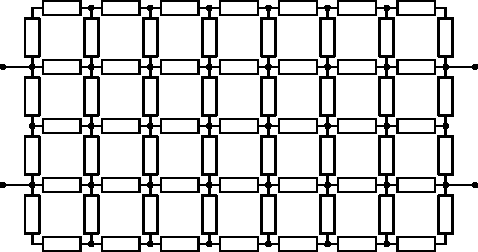
\includegraphics[width=0.7\linewidth]{resistor_grid.pdf}
    \captionof{figure}{Pasivní dvojbran v podobě husté vodivostní sítě}
    \label{ES:fig_res_grid}
    \par}       
    \vspace{1em}

  Na první pohled se zdá, že obě topologie využívají natolik odlišných matematických postupů, že
  spolu tyto disciplíny nijak nesouvisí. Opak je pravdu. Mezi oběma panuje hluboký vztah, obě
  vycházejí ze stejných základů. Vysvětlení lze hledat na obr. \ref{ES:fig_res_grid}. Je zde
  nakreslen \emph{přenosový dvojbran} se zcela obecnou vnitřní strukturou, která může mít např.
  podobu husté vodivostní\footnote{V magnetických obvodech je psychologicky výhodnější pracovat s
  magnetickými vodivostmi než s magnetickými odpory (reluktancemi). Permeabilita má totiž význam
  \emph{měrné magnetické vodivosti}} sítě, ve které mají jednotlivé vodivosti nahodile různé
  hodnoty. S ohledem na dobře známé analogie je lhostejné, zda se jedná o \emph{elektrický} nebo
  \emph{magnetický} obvod. Nakreslený obvod je zcela určitě \emph{diskrétní}, bude tedy řešen
  některou klasickou diskrétní metodu, např. metodou smyčkových proudů nebo metodou uzlových
  napětí. Výpočtem zjistíme, že z pohledu vstupní a výstupní brány má dvojbran konkrétní přenosové
  parametry (napěťový přenos naprázdno, proudový přenos nakrátko, vstupní impedanci naprázdno,
  nakrátko, atd.) Učiňme následující myšlenkový pokus: vodivostní síť budem neustále zjemňovat.
  Tj., ve směru vodorovném i svislém budeme zvyšovat počty prvků, ale tak, aby celková vodivost na
  jednotku délky zůstávala v dané oblasti \emph{konstantní}. Výsledkem zjemňování bude v limitním
  případě vznik \emph{spojité} vodivé desky (např. izolační podložka nastříkaná elektricky vodivým
  odporovým lakem). Mezi původním diskrétním obvodem a deskou zřejmě platí následující souvislosti:
  \begin{itemize}[noitemsep]
    \item Původní diskrétní vodivosti byly nahodile různé \(\longrightarrow\) deska bude
          \emph{nehomogenní, anizotropní}.
    \item Původní diskrétní vodivosti byly stejně velké ve směru \emph{x} a stejně velké (ale s
          jinou hodnotou ve směru \emph{y}) \(\longrightarrow\) deska bude \emph{homogenní
          anizotropní}.
    \item Všechny diskrétní vodivosti měly stejnou hodnotu \(\longrightarrow\) deska bude
          \emph{homogenní, izotropní}.
  \end{itemize}
  
  Intuitivně tušíme, že vytvořená \emph{spojitá} deska\footnote{Uvedený příklad se týká
  dvojrozměrné desky. Příklad lze jistě zobecnit na trojrozměrné objekty (lze si představit
  krabici naplněnou vodivým grafitovým práškem, do které zavedeme čtyři bodové elektrody).} bude mít
  všechny přenosové parametry číselně shodné s původním \emph{diskrétním} obvodem. Přitom ale u
  desky nelze tyto parametry určit klasickými diskrétními metodami (nelze určit matici obvodu). Je
  nutný přechod od diskrétních operací k operacím integrálním, tedy od topologie \emph{diskrétních
  útvarů} k topologii \emph{spojitých útvarů}. Z uvedeného myšlenkového pokusu plyne, že v
  \emph{limitním případě} velmi jemné sítě musí dát diskrétní i spojité operace stejný kvantitativní
  výsledek. Na tomto poznatku je založeno přibližné řešení spojitých prostorových polí
  \emph{metodami konečných prvků}.
  
  Především jsme ovšem chtěli ukázat, že mezi diskrétními a spojitými topologickými metodami není
  zásadního rozdílu, obě vycházejí ze stejných základů a v limitním případě spolu splývají. 
  
  \section{Topologie diskrétních útvarů}\label{teo:IchapIIIsecI}
    Cílem této kapitoly je především vysvětlit \emph{pricnip reciprocity} v pasivních elektrických
    obvodech a pomocí něho odvodit \emph{počet stupňů volnosti} elektrických obvodů. Zvláštním
    případem obvodu je \emph{pasivní přenosový dvojbran}, u kterého bude dokázáno, že má vždy
    \emph{tři stupně volnosti}. Tento poznatek má totiž mimořádný význam v teorii
    \emph{transformátorů}, který je právě typickým představitelem přenosového dvojbranu. V
    kapitolách zabývajících se transformátorem - především jeho náhradním zapojením - se budeme
    odvolávat na výsledky získané v této kapitole. 
    
    \subsection{Základní pojmy teorie grafů}\label{teo:IchapIIIsecIsubI}
      Názvosloví a základní pojmy teorie grafů lze shrnout do následujících bodů:
      \begin{itemize}[noitemsep]
        \item Základním pojmem je \emph{graf} (graf orientovaný, neorientovaný). Graf je vlastně
              „schéma“ příslušného obvodu s vynechanými obvodovými prvky.
        \item Graf sestává z \emph{uzlů} a \emph{hran}.
        \item Uzel je spojení alespoň tří hran\footnote{Spojení dvou hran je elektrický bod, 
              nikoli uzel.}.
        \item Hrana může být \emph{orientovaná} (je jí přiřazen směr), \emph{neorientovaná} (nemá
              přiřazen směr). V elektrotechnice se používají výhradně neorientované hrany - tedy i
              grafy (vlastnosti obvodových prvků R, L, C jsou nezávislé na směru proudu).
        \item \emph{Úplný strom}: nepřerušená celistvá soustava nejmenšího počtu hran, která spojuje
              všechny uzly grafu.
        \item \emph{Nezávislá hrana}: hrana nepatřící do úplného stromu.
        \item \emph{Nezávislá smyčka}: uzavřená smyčka, která musí obsahovat nezávislou hranu, tj.
              hranu nepatřící do úplného stromu.
        \item Nezávislých smyček je tolik, kolik je nezávislých hran.
      \end{itemize}
     
      Označme v grafu:
       \begin{itemize}[noitemsep]
         \item Počet uzlů:  \(q +1\)
      \item Počet hran úplného stromu:  \(q\)
      \item Počet hran (počet neznámých proudů):  \(p\)
      \item Počet nezávislých hran (nezávislých smyček):  \(n=p-q\)
      \end{itemize}
      
      U složitých obvodů je hledání \(n\) nezávislých smyček obtížné. Proto se k tomuto účelu 
      používá úplný strom, jehož nalezení je snadné. Nezávislé hrany jsou ty, které \emph{nepatří} 
      do úplného stromu. Každou nezávislou hranou pak musí procházet alespoň jedna nezávislá 
      smyčka. Všechny pojmy budou ukázány na konkrétním příkladu.
      
      Řešením obvodu se rozumí: Nalezení všech \(p\) neznámých proudů ve všech \(p\) hranách.
      Principiálně se vždy jedná o řešení soustavy \(p\) rovnic o \(p\) neznámých proudech.
      
      K řešení lze použít tři metody:
      \begin{itemize}[noitemsep]
       \item \textbf{Metoda založená na přímém použití I. a II. Kirchhoffova 
             zákona}\footnote{Gustav Robert Kirchhoff (1824-1887), německý fyzik, působil na 
             univerzitách v Heidelbergu a v Berlíně. I. a II. KZ objevil r. 1845 ještě jako 
             student. Dále se zabýval spektroskopií, tepelnou radiací černého tělesa, 
             spoluobjevitel Cesia a Rubidia. Žák F. E. Neumanna.}.
             Je nejméně efektivní, vede na nejrozsáhlejší soustavu \(p\) rovnic o \(p\) neznámých.
       \item \textbf{Metoda smyčkových proudů} (\emph{Mesh Currents Matrix Method}), Maxwellova 
             metoda. Vede na soustavu pouze \(n\) rovnic o \(n\) neznámých smyčkových 
             proudech\footnote{Ze smyčkových proudů lze skutečné proudy snadno vyřešit pomocí 
             doplňkových rovnic sestavených pomocí I. KZ.}. Vezmeme-li v úvahu nejsložitější obvod, 
             ve kterém je každá dvojice uzlů spojena hranou, pak bude:
             \begin{equation}\label{ES:eq_topol00}
               n=p-q=\frac{q(q-1)}{2},
             \end{equation}
             což je  podstatně méně rovnic než \(p\).
       \item \textbf{Metoda uzlových napětí} (\emph{Node Voltages Matrix Method}). Je to metoda 
             nejefektivnější, protože vede na nejmenší soustavu pouze \(q\) rovnic. Metoda je 
             založena na přepočtu všech napětí zdrojů na ekvivalentní zdroje proudové. Z takto 
             určených proudů a ze známých obvodových impedancí je pak možno určit napěťové úbytky 
             na každé impedanci, tedy i napětí všech \(q\) proti zvolenému uzlu referenčnímu.
      \end{itemize}
      
      % --------example: Metoda smyčkových proudů ------------
      % \label{TEO:exam015}
      % !TeX spellcheck = cs_CZ
\begin{example}\label{TEO:exam015}
  Metodou smyčkových proudů vyřešme obvod na obr. \ref{es:fig_patocka_topol02}. Řešením se rozumí 
  nalezení velikosti všech šesti proudů \(I_1\), až \(I_6\). Napětí \(U_1\), \(U_2\), \(U_3\) 
  považujme za známá. Příklad bude řešen jen obecně, nejsou zadána konkrétní čísla. Smyslem 
  příkladu je pouze sestavení \(\mathbb{Z}\)-matice obvodu a ukázka kvalitativních vlastností této 
  matice.
  
   {\centering  
    \begin{tabular}{c}
        \includegraphics[width=0.7\linewidth]{patocka_topol02a.png}  \\
        \includegraphics[width=0.7\linewidth]{patocka_topol02b.png}
    \end{tabular}
    \captionsetup{type=figure}
    \captionof{figure}{a) Řešený obvod, b) Úplný strom (silné čáry) a k němu příslušející soustava 
             třech nezávislých smyček \(A\), \(B\), \(C\) se zvolenými směry smyčkových 
             proudů. Každá ze tří nezávislých smyček \(A\), \(B\), \(C\) prochází alespoň 
             jednou nezávislou hranou (slabé čáry), která nepatří do úplného stromu. 
             \cite[s.~43]{Patocka4}} 
    \label{es:fig_patocka_topol02}
  \par}
  
  Obvod má následující parametry:
  \begin{itemize}\addtolength{\itemsep}{-0.2\baselineskip}
   \item Počet uzlů: \(q + 1 = 4\)
   \item Počet hran úplného stromu: \(q = 3\) (tři silně vytažené čáry)
   \item Počet hran (počet neznámých proudů): \(p = 6\)
   \item Počet nezávislých smyček (nezávislých hran): \(n=p-q=3\)
  \end{itemize}
  
  Pro tři nezávislé smyčky \(A\), \(B\), \(C\) lze sestavit soustavu tří rovnic o třech nově 
  zavedených neznámých fiktivních smyčkových proudech \(I_A\), \(I_B\), \(I_C\). Celková napájecí 
  napětí v každé smyčce jsou označena \(U_A\), \(U_B\), \(U_C\):
  \begin{align}\label{ES:eq_topol01}
    U_A &= U_1-U_3 = (Z_1 + Z_3)I_A +Z_5(I_A - I_C)           \nonumber\\
    U_B &= U_1     = (Z_2 + Z_4)I_B+Z6(I_B + I_C)             \nonumber\\
    U_C &= U_3     = (Z_7 + Z_8)I_C+Z_5(I_C - I_A)+Z_6(I_B+I_c)  
  \end{align}
  Přičemž zřejmě platí:
  \begin{subequations}
    \begin{align}\label{ES:eq_topol02}
     I_1 &= I_A,       \qquad\quad\; I_3 = I_A - I_C,                   \\
     I_4 &= I_B + I_C, \quad I_5 = I_C, \quad I_6 = I_C
    \end{align}
    \end{subequations}
  Pravé strany v soustavě rovnic (\ref{ES:eq_topol01}) uspořádáme podle smyčkových proudů do   
  matice ve tvaru tvaru
  \begin{equation}\label{ES:eq_topol03}
   \left(
     \begin{array}{cccc}
       Z_1+Z_3+Z_5  &              &-Z_5  \\
                    & Z_2+Z_4+Z_6  & Z_6  \\
               -Z_5 & Z_6          & Z_5+Z_6+Z_7+Z_8 
     \end{array}
   \right) 
  \end{equation}
  Další postup by byl následující: \emph{Cramerovým pravidlem} rutinně vyřešit tuto soustavu tří 
  rovnic pro tři neznámé smyčkové proudy a dodatečně dopočítat dvě rovnice (\ref{ES:eq_topol02}). 
  Zbývající čtyři identity v soustavě (\ref{ES:eq_topol02}) není nutno počítat. Tím by byl obvod 
  vyřešen. Smyslem příkladu však nebylo vlastní řešení, nýbrž konkrétní ukázka velice zajímavého 
  jevu: matice (\ref{ES:eq_topol03}) je symetrická podle hlavní diagonály. Symetrie matice je 
  důsledkem principu reciprocity, který bude diskutován v následujících kapitolách.
\end{example}  
      %-------------------------------------------------------
      
    \subsection{Princip reciprocity v pasivních lineárních 
    obvodech}\label{teo:IchapIIsecIsubII}
      Zdůrazněme, že princip reciprocity platí pouze v \emph{pasivních} obvodech, tj. v obvodech, 
      které neobsahují vnitřní (skryté) zdroje napětí nebo proudu. Příklad uvedený v předchozí 
      kapitole slouží jako názorná ukázka principu reciprocity \emph{lineárního} elektrického 
      obvodu. Matice (\ref{ES:eq_topol03}) řešeného obvodu je totiž \emph{symetrická} podle 
      \emph{hlavní diagonály}. Nejedná se o náhodu, podobnou diagonální symetrii bude vykazovat 
      každá \(\mathbb{Z}\)-matice nebo \(\mathbb{Y}\)-matice libovolného pasivního obvodu. Bude-li 
      obvod řešen např. metodou I. KZ a II. KZ, pak bude matice nejrozsáhlejší, bude mít rozměr 
      \(p\times p\), kde \(p\) je počet hran (počet neznámých proudů):
      \begin{equation}\label{ES:eq_topol04}
        \left(
          \begin{array}{ccccc}
             z_{1,1}    &  z_{1,2}   & \ldots & z_{1,p-1}   & z_{1,p}   \\
             z_{2,1}    &  z_{2,2}   & \ldots & z_{2,p-1}   & z_{2,p}   \\
             \vdots     &  \vdots    & \ddots & \vdots      &\vdots     \\
             z_{p-1,1}  &  z_{p-1,2} & \ldots & z_{p-1,p-1} & z_{p-1,p} \\
             z_{p,1}    &  z_{p,2}   & \ldots & z_{p,p-1}   & z_{p,p}   \\
          \end{array}
        \right)
     \end{equation}
      
      Tato matice bude určitě opět symetrická podle hlavní diagonály. Diagonální symetrie 
      \(\mathbb{Z}\)-matic i \(\mathbb{Y}\)-matic je nejvýznamnější a nejobecnější vlastností všech 
      pasivních obvodů. Matematicky lze tuto symetrii zapsat ve tvaru
      \begin{equation}\label{ES:eq_topol05}
        z_{ij} = z_{ji} \qquad\text{případně}\qquad y_{ij} = y_{ji}
      \end{equation}
      Obě rovnice (\ref{ES:eq_topol05}) vyjadřují princip reciprocity, který můžeme slovně 
      formulovat takto: a) Přenosová impedance naprázdno měřená podle obr. 
      \ref{es:fig_patocka_topol03a} mezi \(r\)-tou a \(y\)-tou hranou obvodu je stejná pro oba 
      směry přenosu:
      \begin{figure}[ht!]
        \centering  
        \subcaptionbox{\label{es:fig_patocka_topol03a}}{\luafigure[0.9]{patocka_topol03a.png}}   \\
        \subcaptionbox{\label{es:fig_patocka_topol03b}}{\luafigure[0.9]{patocka_topol03b.png}}
        \caption{Měření přenosových parametrů: a) \textbf{impedancí naprázdno} \(Z_{ij,0}\) a 
                 \(Z_{ji,0}\) v obou směrech mezi \(i\)-tou a \(j\)-tou hranou obvodu. Obvod je 
                 napájen zdrojem proudu a měříme napětí. Obě měření musí dát stejný výsledek. b)  
                 \textbf{admitancí nakrátko} \(Y_{ij,K}\) a \(Y_{ji,K}\) v obou směrech mezi 
                 \(i\)-tou a \(j\)-tou hranou obvodu. Obvod je napájen zdrojem napětí a měříme 
                 proud. Obě měření musí dát stejný výsledek. \cite[s.~45]{Patocka4}} 
        \label{es:fig_patocka_topol03}
      \end{figure}
      
      Princip reciprocity neplyne z žádných vyšších fyzikálních zákonů (např. ze zákona zachování 
      energie, náboje atd.). Sám je totiž samostatným základním zákonem vyjadřujícím určitou 
      topologickou kvalitu („geometrickou kvalitu“) každého elektrického obvodu.
      
      Na závěr zdůrazněme, že u \emph{lineárních} obvodů jsou všechny maticové prvky \(z_{ij}\) 
      \emph{konstantami} nezávislými na proudech \(I_1\), až \(I_p\), a podobně všechny maticové 
      prvky \(y_{ij}\). jsou \emph{konstantami} nezávislými na napětích \(U_1\), až \(U_p\). Na 
      rozdíl od nelineárních obvodů v následující kapitole.
      
    \subsection{Princip reciprocity v pasivních nelineárních obvodech}\label{teo:IchapIIIsecIsubIII}
      V této kapitole ukážeme, že princip reciprocity platí i v případě \emph{nelineárních} obvodů. 
      Musí se však jednat opět o pasivní obvody, tj. obvody, které neobsahují vnitřní zdroje.
      
      Každá \(\mathbb{Z}\)-matice nebo \(\mathbb{Y}\)-matice libovolného \emph{nelineárního} obvodu 
      je opět \emph{symetrická podle hlavní diagonály}. Ale - na rozdíl od lineárních obvodů - 
      maticové prvky \(z_{ij}\), \(y_{ij}\) nebudou konstantami, nýbrž budou \emph{mnohorozměrnými 
      funkcemi} vnějších budicích veličin. Konkrétně maticové prvky \(z_{ij}(I_1\ldots I_p)\) budou 
      funkcemi proudů \(I_1\), až \(I_p\) a maticové prvky \(y_{ij}(U_1\ldots U_p)\) budou 
      mnohorozměrnými funkcemi napětí \(U_1\), až \(U_p\). Např. \(\mathbb{Z}\)-matice bude mít 
      tvar:
        \begin{equation*}
          \left(
            \begin{array}{ccccc}
              z_{1,1}(I_1\ldots I_p)     &  z_{1,2}(I_1\ldots I_p)   & \ldots & 
              z_{1,p-1}(I_1\ldots I_p)   &  z_{1,p}(I_1\ldots I_p)                   \\
              z_{2,1}(I_1\ldots I_p)     &  z_{2,2}(I_1\ldots I_p)   & \ldots & 
              z_{2,p-1}(I_1\ldots I_p)   &  z_{2,p}(I_1\ldots I_p)                   \\
              \vdots      &  \vdots      &  \ddots     & \vdots      & \vdots        \\
              z_{p-1,1}(I_1\ldots I_p)   &  z_{p-1,2}(I_1\ldots I_p) & \ldots & 
              z_{p-1,p-1}(I_1\ldots I_p) &  z_{p-1,p}(I_1\ldots I_p)                 \\
              z_{p,1}(I_1\ldots I_p)     &  z_{p,2}(I_1\ldots I_p)   & \ldots & 
              z_{p,p-1}(I_1\ldots I_p)   &  z_{p,p}(I_1\ldots I_p)                   \\
            \end{array}
          \right)
        \end{equation*}
      
      Symetrii \(\mathbb{Z}\)-matic a \(\mathbb{Y}\)-matic podle hlavní diagonály lze matematicky 
      zapsat ve tvaru
      \begin{subequations}
        \begin{align}\label{ES:eq_topol06}
          z_{ij}(I_1\ldots I_p) &= z_{ji}(I_1\ldots I_p) \\
          \shortintertext{případně}
          y_{ij}(U_1\ldots U_p) &= y_{ji}(U_1\ldots U_p)
        \end{align}
      \end{subequations}
      
      Zdůrazněme, že klasická teorie elektrických obvodů připouští platnost principu reciprocity 
      pouze u \emph{lineárních} obvodů, např. Někdy bývá dokonce explicitně vysloveno mylné 
      tvrzení, že v \emph{nelineárních} obvodech princip neplatí. Proto nyní dokážeme, že princip 
      reciprocity je možno rozšířit i na obvody nelineární. Důkaz lze konstruovat následovně:
     
      
      \begin{enumerate}[noitemsep]
        \item Předpokládejme nelineární obvod, ale buzený signály o \emph{velmi malé} amplitudě.
        \item Bude-li se amplituda všech signálů limitně blížit nule, lze obvod 
              \emph{linearizovat} v určitém stejnosměrném pracovním bodu, tj. všechny nelineární 
              převodní funkce \(z_{ij}(I_1\ldots I_p)\) lze nahradit převodními konstantami 
              \(z_{ij}\) jejichž velikost je dána parciálními derivacemi původní funkce v onom 
              pracovním bodu (jedná se o běžný linearizační postup).
        \item Když jsme takto obvod \emph{linearizovali}, musí se pro limitně malé signály chovat 
              jako obvod \emph{lineární} - a to se všemi důsledky z toho plynoucími, tedy včetně 
              existence principu reciprocity.
        \item Nutnou a postačující podmínkou platnosti tvrzení 3) je splnění rovnice 
              (\ref{ES:eq_topol06}).
      \end{enumerate}
      Konec důkazu.
      
      Poznatek, že princip reciprocity platí i v \emph{nelineárních} elektrických soustavách, má 
      velký význam při vytváření matematických modelů nelineárních soustav: jednak bude model 
      jednodušší (menší počet převodních funkcí), jednak máme částečnou kontrolu jeho správnosti. 
      Princip reciprocity splňují nejen \emph{lineární} a \emph{nelineární} soustavy elektrické, 
      nýbrž všechny fyzikální soustavy. Jedná se o jeden z nejobecnějších fyzikálních zákonů 
      topologického charakteru\footnote{Například Einstein předpokládal platnost principu 
      reciprocity i ve své teorii gravitace. Po určitých úvahách totiž postuloval diagonální 
      symetrii Riemannova tenzoru křivosti čtyřrozměrného časoprostoru. Tento tenzor druhého řádu 
      má tvar matice o rozměru \(4\times4\). Obsahuje tedy 16 členů, 16 čtyřrozměrných 
      metrických funkcí \(g_{ij}(x, y, z, ct)\). Z postulované symetrie plyne, že pouze 10 z nich 
      je různých (\(10 = 4+3+2+1\)). Řešení gravitačního pole tedy spočívá ve vyřešení soustavy 10 
      nelineárních parciálních diferenciálních rovnic o 10 neznámých funkcích \(g_{ij}(x, y, z, 
      ct)\). Proto se jedná o velmi obtížnou úlohu.}.
      
    \subsection{Počet stupňů volnosti pasivního mnohopólu}\label{teo:IchapIIIsecIsubIV}
      Obecný mnohopól je nakreslen na obr. \ref{es:fig_patocka_topol04}. Nechť má tento obvod \(r\) 
      vnějších svorek. Pak zřejmě celkový počet všech možných dvojic svorek, tj. všech možných 
      napětí v obvodu je roven
      \begin{equation}\label{ES:eq_topol07}
        s=(r-1) + (r-2) + (r-2) + \ldots + 3 + 2 + 1 = \frac{r(r-1)}{2}.
      \end{equation}
      \begin{figure}[ht!]   %\ref{es:fig_patocka_topol04}
        \centering
        \includegraphics[width=0.6\linewidth]{patocka_topol04.png}
        \caption{Obecný \(r\)-pól \cite[s.~46]{Patocka4}.}
        \label{es:fig_patocka_topol04}
      \end{figure}
      Zřejmě však stačí připojit \((r-1)\) vnějších nezávislých napájecích napětí (napěťových 
      zdrojů) a všechna zbývající napětí mezi libovolnými dvojicemi svorek jsou pak plně 
      definována, neboť mezi napětími platí II. KZ. Podobně stačí měřit \((r-1)\) vnějších proudů, 
      zbývající \(r\)-tý proud je na nich lineárně závislý (\(r\)-pól se chová jako uzel, mezi 
      jehož proudy platí 1. KZ). Vnější chování \(r\)-pólu je tedy plně popsáno vektorem \((r-1)\) 
      napětí a vektorem \((r-1)\) proudů. Odtud plyne, že vnější vlastnosti \(r\)-pólu jsou plně 
      definovány čtvercovou \(\mathbb{Z}\)-maticí nebo \(\mathbb{Y}\)-maticí o rozměru 
      \((r-l)\times(r-1)\). Uvedeme např. \(\mathbb{Z}\)-matici:  
      \begin{equation}\label{ES:eq_topol08}
        \left(
          \begin{array}{ccccc}
            z_{1,1}    &  z_{1,2}   & \ldots & z_{1,r-2}   & z_{1,r-1}    \\
            z_{2,1}    &  z_{2,2}   & \ldots & z_{2,r-2}   & z_{2,r-1}    \\
            \vdots     &  \vdots    & \ddots & \vdots      &\vdots        \\
            z_{r-2,1}  &  z_{r-2,2} & \ldots & z_{r-2,r-2} & z_{r-2,r-1}  \\
            z_{r-1,1}  &  z_{r-1,2} & \ldots & z_{r-1,r-2} & z_{r-1,r-1}  \\
          \end{array}
        \right)
      \end{equation}
      
      Mnohopól je \emph{zvláštním případem} obecného elektrického obvodu. V každém elektrickém 
      obvodu platí princip reciprocity, proto musí platit i v případě \(r\)-pólu. Odtud plyne, že 
      jeho matice (\ref{ES:eq_topol08}) musí být symetrická podle hlavní diagonály. To znamená, že 
      z celkového počtu \((r-1)^2\) maticových prvků je různých pouze \((r-1) + (r-2) + (r-3) +... 
      + 3 + 2 + 1\). Jinak řečeno, počet stupňů volnosti s libovolného pasivního \(r\)-pólu je dán 
      rovnicí (\ref{ES:eq_topol07}). Význam počtu stupňů volnosti \(s\) je mimořádný. Lze totiž 
      dokázat následující větu.
      
      \begin{lemma}\label{ES:lem_topol01}
        Z hlediska vnějšího chování lze každý libovolně složitý \(r\)-pól nahradit \(r\)-pólem
        ekvivalentním sestaveným pouze z tolika impedancí, kolik stupňů volnosti má původní obvod, 
        tedy sestaveným z \(s = \frac{r(-1)}{2}\) impedancí. Přičemž těchto \(s\) impedancí musí 
        být zapojeno ve shodě s obr. \ref{es:fig_patocka_topol05}, tj. každá dvojice svorek musí 
        být propojena jednou impedancí.
        \begin{figure}[ht!]
          \centering  
          \subcaptionbox{\label{es:fig_patocka_topol05a}}{\luafigure[0.11]{patocka_topol05a.png}}
          \subcaptionbox{\label{es:fig_patocka_topol05b}}{\luafigure[0.18]{patocka_topol05b.png}}
          \subcaptionbox{\label{es:fig_patocka_topol05c}}{\luafigure[0.25]{patocka_topol05c.png}}
          \subcaptionbox{\label{es:fig_patocka_topol05d}}{\luafigure[0.25]{patocka_topol05d.png}}
          \caption{Příklady náhrady obecného r-pólu ekvivalentním r-pólem: a) dvojpól, b) trojpól,
                   c) čtyřpól, d) pětipól. Číslo \(s\) souhlasí s rovnicí (\ref{ES:eq_topol07}).
                   \cite[s.~47]{Patocka4}} 
          \label{es:fig_patocka_topol05}
        \end{figure}
      \end{lemma}
      Důkaz věty bude naznačen v následující kapitole.
      
    \subsection{Počet stupňů volnosti pasivního čtyřpólu}\label{teo:IchapIIIsecIsubV}
      Důkaz věty \ref{ES:lem_topol01} ukážeme na případu čtyřpólu. Systematická konstrukce důkazu 
      je znázorněna na obr. \ref{es:fig_patocka_topol06}. Původní složitý čtyřpól začneme 
      dovolenými ekvivalentními úpravami měnit tak, abychom postupně snižovali celkový počet 
      odporů. Začneme-li např. v levém horním rohu, postup bude následující:
      \begin{figure}[ht!]   %\ref{es:fig_patocka_topol06}
        \centering
        \includegraphics[width=0.95\linewidth]{patocka_topol06.png}
        \caption{Postupná náhrada složitého čtyřpólu čtyřpólem ekvivalentním, sestaveným ze šesti
                 impedancí. \cite[s.~48]{Patocka4}.}
        \label{es:fig_patocka_topol06}
      \end{figure}
      \begin{enumerate}[noitemsep]
        \item Dva černě vyznačené odpory sečteme - počet prvků klesl o jedničku.
        \item V rohu vznikl trojúhelník ze tří černě vyznačených odporů.        
        \item Vzniklý černý trojúhelník přeměníme pomocí dobře známé transfigurace na hvězdu.
        \item Po vzniku hvězdy se objeví dva odpory zapojené do série (černý a bílý). Odpory 
              sečteme - počet prvků klesl o další jedničku.
        \item Po sečtení odporů se objeví dvě černě vyznačené hvězdy ležící vedle sebe.
        \item Obě hvězdy přeměníme pomocí transfigurace na dva trojúhelníky (tato operace již není 
              nakreslena).
        \item Po vzniku trojúhelníků se objeví na sousedících stranách trojúhelníků dva odpory 
              zapojené paralelně. Odpory sečteme, čímž počet prvků klesne o další jedničku.
        \item Postupným střídáním transfigurací z hvězd na trojúhelníky a opačně, z trojúhelníků na 
              hvězdy, neustále snižujeme počet prvků o jedničku.
        \item Algoritmus lze neustále opakovat až do okamžiku, kdy nám zbude šest odporů zapojených 
              do můstku podle obrázku. Toto zápojem již nelze žádným postupem více minimalizovat.
      \end{enumerate}
      Konec důkazu.
      
      Ve zvláštním případě, jsou-li svorky \(b, d\) původního čtyřpólu vodivě spojeny (jedná se pak 
      o trojpól), výsledkem algoritmu bude \(T\)-článek sestavený pouze ze tří odporů a ten lze 
      případně přepočítat pomocí transfigurace hvězda-trojúhelník na rovnocenný 
      \(\Pi\)-článek\footnote{Lze dokázat, že transfigurace \emph{hvězda-trojúhelník} je 
      uskutečnitelná právě pouze pro \emph{trojpól}. Pro všechny ostatní r-póly, u nichž \(r > 3\), 
      realizovatelná \emph{není}. Jev není náhodný, úzce souvisí se \emph{třemi stupni volnosti}.}.
      
      V obecném případě je ale výsledkem zjednodušovacího algoritmu vždy obvod sestavený ze šesti 
      odporů podle obr. \ref{es:fig_patocka_topol07}. Obvod lze nakreslit ve tvaru křížového článku 
      nebo ve tvaru můstku zatíženého na vstupu i výstupu impedancemi. Křížový článek a zatížený 
      můstek jsou obvody topologicky totožné.
      \begin{figure}[ht!]
        \centering  
        \includegraphics[width=0.95\linewidth]{patocka_topol07.png}
        \caption{Náhrada libovolné složitého čtyřpólu čtyřpólem ekvivalentním.
                \cite[s.~48]{Patocka4}} 
        \label{es:fig_patocka_topol07}
      \end{figure}
      
    \subsection{Počet stupňů volnosti pasivního dvojbranu}\label{teo:IchapIIIsecIsubVI}
      Tuto a následující kapitoly je nutno chápat jako důležitou teoretickou připravu, bez níž není 
      možno plně pochopit teorii transformátoru uvedenou v kapitole 17.
      
      Přenosový dvojbran je zvláštním případem čtyřpólu. Čtyř\-pól podle obr. 
      \ref{es:fig_patocka_topol07} může být považován za přenosový dvojbran, pokud nás nebudou 
      zajímat podélná napětí mezi svorkami \(a-c\), \(a-d\), \(b-c\), \(b-d\). Pak se z něj stává 
      dvojbran podle obr. \ref{es:fig_patocka_topol08}, který má pouze dvě brány, z nichž jednu 
      považujeme za vstupní a druhou za výstupní.
      
      Vnější chování dvojbranu je tedy popsáno vektorem \emph{dvou napětí} a vektorem \emph{dvou 
      proudů}. Vnější vlastnosti dvojbranu jsou proto plně definovány čtvercovou 
      \(\mathbb{Z}\)-maticí nebo  \(\mathbb{Y}\)-maticí o rozměru \(2\times2\). Uvedeme např. 
      \(\mathbb{Z}\)-matici:
      \begin{equation}\label{ES:eq_topol09}
        \left(
          \begin{array}{c}
            U_1 \\ U_2   
           \end{array}
        \right)
        =
        \left(
        \begin{array}{cc}
          z_{11}    &  z_{12}   \\
          z_{21}    &  z_{22}   
        \end{array}
        \right)
        \cdot
        \left(
          \begin{array}{c}
            I_1 \\ I_2 
          \end{array}
        \right).         
      \end{equation}
      
      \begin{figure}[ht!]
        \centering  
        \includegraphics[width=0.5\linewidth]{patocka_topol08.png}
        \caption{Označení veličin vstupní a výstupní brány dvojbranu. \cite[s.~49]{Patocka4}} 
        \label{es:fig_patocka_topol08}
      \end{figure}
      
      Pasivní dvojbran musí splňovat princip reciprocity. Jeho matice tedy musí být symetrická 
      podle hlavní diagonály, proto musí platit \(z_{12} = z_{21}\). To znamená, že z celkového 
      počtu čtyř maticových prvků jsou pouze \emph{tři prvky různé}. Toto zjištění je přímým 
      důkazem následující věty:
      \begin{lemma}\label{ES:lem_topol02}
         Každý pasivní přenosový dvojbran má pouze \emph{tři stupně volnosti}. Proto může být vždy 
         nahrazen ekvivalentním \emph{trojpólem} ve tvaru \(T\)-článku (nebo \(\Pi\)-článku) 
         sestaveným ze tří impedancí. Proto jsou všechny přenosové vlastnosti dvojbranu plně 
         definovány:
         \begin{itemize}[noitemsep]
            \item buď \emph{trojicí} parametrů obvodových (u transformátoru např. \(L_1, L_2, M\)),
            \item nebo \emph{trojicí} parametrů přenosových (např. \(Z_{vst_0}\), \(Z_{vst_K}\),    
                  \(K_{U_{21,0}}\)),
            \item nebo \emph{trojicí} maticových koeficientů (např. \(z_{11}, z_{21}, z_{22}\)).
          \end{itemize}
      \end{lemma}
      
    \subsection{Popis dvojbranu pomocí matic typu Z, Y, H}\label{teo:IchapIIIsecIsubVII}
      Vnější chování každého dvojbranu lze popsat maticí o dimenzi \(2\times2\). Jedná se tedy o 
      soustavu dvou rovnic o \emph{čtyřech} vnějších veličinách \(U_1, U_2, I_1, I_2\). Má-li být 
      soustava řešitelná, je nutno některé \emph{dvě veličiny zvolit za neznámé} a zbylé dvě 
      považovat při výpočtu za \emph{známé}. Existuje šest různých dvojic vybraných ze čtveřice, 
      tomu odpovídá šest typů matic. Kromě známé \(\mathbb{Z}\)-matice a \(\mathbb{Y}\)-matice 
      existují další čtyři hybridní \(\mathbb{H}\)- matice:
      \begin{align*}
        \shortintertext{\texttt{matice }\(\mathbb{Z}\):}
          \left(
            \begin{array}{c}
              U_1 \\ U_2   
            \end{array}
          \right)
          &=
          \left(
            \begin{array}{cc}
              z_{11}    &  z_{12}   \\
              z_{21}    &  z_{22}   
            \end{array}
          \right)
          \cdot
          \left(
            \begin{array}{c}
              I_1 \\ I_2 
            \end{array}
          \right)                                                 \\
        \shortintertext{\texttt{matice }\(\mathbb{H}_K\):}
          \left(
            \begin{array}{c}
              U_1 \\ I_1   
            \end{array}
            \right)
            &=
            \left(
              \begin{array}{cc}
                h_{K_{11}}    &  h_{K12}   \\
                h_{K_{21}}    &  h_{K22}   
              \end{array}
            \right)
            \cdot
            \left(
              \begin{array}{c}
                U_2 \\ I_2 
              \end{array}
          \right)                                               \\
        \shortintertext{\texttt{matice }\(\mathbb{H}_I\): }
          \left(
            \begin{array}{c}
              U_1 \\ I_2   
            \end{array}
          \right)
          &=
          \left(
            \begin{array}{cc}
              h_{I_{11}}    &  h_{I_{12}}   \\
              h_{I_{21}}    &  h_{I_{22}}   
            \end{array}
          \right)
          \cdot
          \left(
            \begin{array}{c}
              I_1 \\ U_2 
            \end{array}
          \right)                                              \\
        \shortintertext{\texttt{matice }\(\mathbb{H}_U\):}
          \left(
            \begin{array}{c}
              I_1 \\ U_2   
            \end{array}
            \right)
            &=
            \left(
              \begin{array}{cc}
                h_{U_{11}}    &  h_{U_{12}}   \\
                h_{U_{21}}    &  h_{U_{22}}   
              \end{array}
            \right)
            \cdot
            \left(
              \begin{array}{c}
                U_1 \\ I_2 
              \end{array}
          \right)                                              \\
        \shortintertext{\texttt{matice }\(\mathbb{H}_N\):}
          \left(
            \begin{array}{c}
              U_2 \\ I_2   
            \end{array}
          \right)
          &=
          \left(
            \begin{array}{cc}
              h_{N_{11}}    &  h_{N_{12}}   \\
              h_{N_{21}}    &  h_{N_{22}}   
            \end{array}
          \right)
          \cdot
          \left(
            \begin{array}{c}
              U_1 \\ I_1 
            \end{array}
          \right)                                               \\
        \shortintertext{\texttt{matice }\(\mathbb{Y}\):}
          \left(
            \begin{array}{c}
              I_1 \\ I_2   
            \end{array}
            \right)
            &=
            \left(
              \begin{array}{cc}
                y_{11}    &  y_{12}   \\
                y_{21}    &  y_{22}
              \end{array}
            \right)
            \cdot
            \left(
              \begin{array}{c}
                U_1 \\ U_2 
              \end{array}
          \right) 
      \end{align*}
      Jednotlivým maticím odpovídají různé matematické modely dvojbranu. Mimořádný význam má 
      hybridní \(\mathbb{H}_U\)-matice vho\-dná pro modely všech dvojbranu napájených zdrojem 
      \emph{napětí} (tedy vhodná pro model transformátoru napětí) a hybridní 
      \(\mathbb{H}_I\)-matice vhodná pro modely všech dvojbranu napájených zdrojem \emph{proudu} 
      (tedy vhodná pro model transformátoru proudu). Kaskádní dopředná matice typu \(\mathbb{H}_K\) 
      a kaskádní zpětná matice typu \(\mathbb{H}_N\) se pro popis transformátoru příliš nehodí.

      
    \subsection{Přenosové parametry dvojbranu}\label{teo:IchapIIIsecIsubVIII}
      Všechny možné přenosové parametry jsou uvedeny v tab. \ref{ES:tab_topol01}. Je jich celkem 
      \num{16}, což není náhoda (\(2^4 = 16\)). Tabulka ukazuje u každého přenosového parametru 
      jeho \emph{elementární} vztah k některému maticovému parametru. Prázdná místa v tabulce by 
      bylo možno zaplnit \emph{složitými} algebraickými vztahy (do tabulky se bohužel nevejdou), 
      každý přenosový parametr se dá totiž vždy vyjádřit pomocí čtveřice parametrů \(z\) nebo \(y\) 
      nebo \(h\) (viz následující příklad). Vztahy lze snadno odvodit s využitím třetí doplňující 
      rovnice \(U_j = 0\) (\emph{brána nakrátko}) nebo \(I_j = 0\) (\emph{brána naprázdno}), kde 
      \(j = 1\) (vstupní brána) nebo \num{2} (výstupní brána). Konkrétní postup plyne z 
      následujícího příkladu.
      \begin{table*}[!t]
        \centering
        \resizebox{0.9\textwidth}{!}{
          \begin{tabular}{|l|l|l|l|l|l|l|l|}
            \hline
            &  & \multicolumn{6}{l|}{{\textbf{Vztah k maticovým parametrům} \(z, h, y\)}} \\ 
            \cline{3-8} 
            \multirow{-2}{*}{\textbf{Přenosový parametr}} & \multirow{-2}{*}{\textbf{Značka}} 
            & \(z\) & \(h_K\) & \(h_I\) & \(h_U\) & \(h_N\) & \(y\) \\ 
            \hline\hline
            vstupní impedance při výstupu naprázdno  
            & \(Z_{vst_0}\) 
                  & \(z_{11}\) & & & & &                      \\
            vstupní impedance při výstupu nakrátko  
            & \(Z_{vst_K}\) 
                  & & & \(h_{I_{11}}\) & & &                  \\
            výstupní impedance při vstupu naprázdno  
            & \(Z_{\text{výst}_0}\) 
                  & \(z_{22}\) & & & \(h_{U_{22}}\) & &       \\
            výstupní impedance při vstupu nakrátko   
            & \(Z_{\text{výst}_K}\) 
                  & & & & & &                                 \\
            přenosová impedance naprázdno (\(\rightarrow\))
            & \(Z_{21_0}\) 
                  & \(z_{21}\) & \(1/h_{K_{21}}\) & & & &     \\
            přenosová impedance naprázdno (\(\leftarrow\))
            & \(Z_{12_0}\) 
                  & \(z_{12}\) & & & & \(1/h_{N_{21}}\) &     \\
            vstupní admitance při výstupu naprázdno 
            & \(Y_{vst_0}\) 
                  & & & & \(h_{U_{11}}\)& &                   \\
            vstupní admitance při výstupu nakrátko  
            & \(Y_{vst_K}\) 
                  & & & & & & \(y_{11}\)                      \\
            výstupní admitance při vstupu naprázdno  
            & \(Y_{\text{výst}_0}\) 
                  & & & \(h_{I_{22}}\) & & &                  \\
            výstupní admitance při vstupu nakrátko  
            & \(Y_{\text{výst}_K}\) 
                  & & & & & & \(y_{22}\)                      \\
            přenosová admitance nakrátko (\(\rightarrow\))
            & \(Y_{21_K}\) 
                  & & \(1/h_{K_{11}}\) & & & & \(y_{21}\)     \\
            přenosová admitance nakrátko (\(\leftarrow\))
            & \(Y_{12_K}\) 
                  & & & & & \(1/h_{N_{12}}\) & \(y_{12}\)     \\
            napěťový přenos naprázdno (\(\rightarrow\))
            & \(K_{U_{21_0}}\) 
                  & & \(1/h_{K_{11}}\) & & \(h_{U_{21}}\) & & \\
            napěťový přenos naprázdno (\(\leftarrow\))
            & \(K_{U_{12_0}}\) 
                  & & & \(h_{I_{12}}\) & & \(1/h_{N_{11}}\) & \\
            proudový přenos nakrátko (\(\rightarrow\))
            & \(K_{I_{21_K}}\) 
                  & & \(1/h_{K_{22}}\) & \(h_{I_{21}}\) & & & \\
            proudový přenos nakrátko (\(\leftarrow\))
            & \(K_{I_{12_K}}\) 
                  & & & & \(h_{U_{12}}\) & \(1/h_{N_{22}}\) & \\
            \hline
          \end{tabular}
        }
        \caption{Přehled všech možných přenosových parametrů dvojbranu.}
        \label{ES:tab_topol01}
      \end{table*}

      % --------example: Metoda smyčkových proudů ------------
      % \label{TEO:exam016}
      % !TeX spellcheck = cs_CZ
\begin{example}\label{TEO:exam016}
  Vyjádřeme pomocí \(y\)-parametrů následující přenosové parametry dvojbranu: vstupní impedance při 
  výstupu naprázdno \(Z_{vst_0}\), \(K_{I_{12_K}}\), \(Z_{12_0}\). 
  
  Řešení:
  \begin{itemize}[noitemsep]
    \item \(Z_{vst_0}\): \(\mathbb{Y}\)-matici doplníme třetí rovnicí \(I_2=0\) (podmínka 
    definující výstup naprázdno):
    \begin{subequations}\label{ES:eq_topol10}
      \begin{align}
        I_1 &= y_{11}U_1 - y_{12}U_2  \\
        I_2 &= y_{21}U_1 - y_{22}U_2  \\
        I_2 &= 0
      \end{align}
    \end{subequations}
    Záporná znaménka v \(\mathbb{Y}\)-matici (tj. v prvních dvou rovnicích) jsou správná, protože 
    směr výstupního proudu \(I_2\) na obr. \ref{es:fig_patocka_topol08} je zvolen v souladu s 
    realitou, tj. v souladu s napětím \(U_2\). Pokud je totiž dvojbran zatížen \emph{pasivní} 
    zátěží, pracující ve \emph{spotřebičovém} režimu, proud \(I_2\) musí z výstupní svorky 
    dvojbranu vytékat, nikoli do ní vtékat\footnote{Směry obou proudů \(I_1\), \(I_2\) lze volit 
    libovolně. V literatuře se obvykle směry proudů volí tak, že oba vtékají do dvojbranu. Důvod je 
    pouze formální, pak totiž budou všechny čtyři maticové koeficienty kladně. Výsledkem je ale 
    nerealistický stav na výstupní bráně, tj. na pasivní zátěži. Proto nebudeme toto značeni 
    používat a směry všech veličin budeme systematicky volit podle obr. 
    \ref{es:fig_patocka_topol08}. Z psychologického hlediska tato volba velmi usnadní budoucí 
    analýzu transformátoru.}. Všimněme si, že jsme získali soustavu tří rovnic o čtyřech neznámých 
    veličinách \(U_1\), \(U_2\), \(I_1\), \(I_2\). Ta je pro \emph{jednotlivé} neznámé neřešitelná. 
    Je však řešitelná pro poměry dvou libovolných proměnných. Ze soustavy lze po algebraických 
    úpravách získat hledanou vstupní impedanci při výstupu naprázdno:
    \begin{equation}\label{ES:eq_topol11}
    Z_{vst_0} = \frac{U_1}{I_1}\Bigg\lvert_{I_2=0} 
    = \frac{y_{22}}{y_{22}y_{11} - y_{12}y_{21}}.
    \end{equation}
    \item \(K_{I_{12_K}}\): \(\mathbb{Y}\)-matici doplníme třetí rovnicí \(U_1 = 0\) (podmínka 
    definující vstup nakrátko). Jedná se o přenos ve zpětném směru (\(\leftarrow\)). Při zpětném 
    přenosu tečou oba proudy na obr. \ref{es:fig_patocka_topol08} obráceným směrem, proto musí mít 
    přiřazena záporná znaménka:
    \begin{equation}\label{ES:eq_topol12}
    K_{I_{12_K}} = \frac{-I_1}{-I_2}\Bigg\lvert_{U_1=0} 
    = \frac{I_1}{I_2}\Bigg\lvert_{U_1=0}
    = \frac{y_{12}}{y_{22}}.
    \end{equation}          
    \item \(Z_{12_0}\): \(\mathbb{Y}\)-matici doplníme třetí rovnicí \(I_1=0\) (podmínka  
    definující vstup naprázdno). Při zpětném přenosu (\(\leftarrow\)) tečou oba proudy na obr. 
    \ref{es:fig_patocka_topol08} obráceným směrem, proto musí mít přiřazena záporná znaménka:
    \begin{equation}\label{ES:eq_topol13}
    Z_{vst_0} = \frac{U_1}{-I_2}\Bigg\lvert_{I_1=0} 
    = \frac{y_{12}}{y_{21}y_{12} - y_{11}y_{22}}.
    \end{equation}
  \end{itemize}
  Tytéž přenosové parametry \(Z_{vst_0}\), \(K_{I_{12_K}}\), \(Z_{12_0}\) je možno vyjádřit pomocí 
  \(z\)-parametrů nebo \(h\)-parametrů. Podobným způsobem by bylo možno doplnit všechna prázdná 
  pole v tab. \ref{ES:tab_topol01}.
\end{example}
  
      %-------------------------------------------------------

      Ze tří stupňů volnosti dvojbranu plyne, že jen některé speciálně vybrané trojice ze
      šestnácti přenosových parametrů jsou na sobě nezávislé, např. \(Z_{vst_0}\),  \(Z_{vst_K}\), 
      \(K_{U_{21_0}}\). Většina parametrů musí být navzájem lineárně závislá. Jako typické příklady 
      lineárních závislostí uveďme:
      \begin{equation*}          %\label{ES:eq_topol14}
        Z_{vst_0} = \frac{1}{Y_{vst_0}}, \quad 
        \frac{Z_{vst_0}}{Z_{vst_K}}=\frac{Z_{\text{výst}_0}}{Z_{\text{výst}_K}}, \quad
        \frac{Z_{vst_0}}{Z_{\text{výst}_0}}=\frac{Z_{\text{vst}_K}}{Z_{\text{výst}_K}}
      \end{equation*}
      Existují i mnohé další, komplikovanější. Z hlediska transformátoru jsou však velmi důležité 
      jiné dvě lineární závislosti:
      \begin{equation}\label{ES:eq_topol15}
        K_{U_{21_0}} = K_{I_{12_K}}, \qquad 
        K_{I_{21_K}} = K_{U_{12_0}}
      \end{equation}
      U transformátoru jsou tyto rovnice všeobecně známy ve smyslu tj. napěťový převod \emph{tam} 
      je stejný jako proudový převod \emph{zpět}. Ze systémového pohledu je však dobré uvědomit si, 
      že:
      \begin{itemize}[noitemsep]
        \item tuto vlastnost mají \emph{všechny} pasivní dvojbrany, např. i obyčejný odporový dělič,
        \item transformátor není žádnou výjimkou,
        \item tzv. převod transformátoru je fyzikálně totožný s pojmem \emph{napěťový přenos 
              naprázdno} nebo \emph{proudový přenos nakrátko}.
      \end{itemize}
      
    \subsection{Princip reciprocity v elektromechanických 
    soustavách}\label{teo:IchapIIsecIsubIX}
      Z hlediska teoretického je velmi zajímavé, že princip reciprocity platí i u všech 
      \emph{elektromechanických měničů} energie. Pohlížíme-li např. na stejnosměrný motor s 
      konstantním buzením jako na „přenosový dvojbran“ s elektrickými veličinami \(u(t)\), \(i(t)\) 
      na elektrické bráně a s mechanickými veličinami \(M(t)\), \(\omega(t)\) na mechanické bráně, 
      pak lze tento systém popsat např. hybridní \(\mathbb{H}\)-maticí ve tvaru
      \begin{subequations}\label{ES:eq_topol16}
        \begin{align}
          u(t) &= Ri(t) + L\der{i(t)}{t} + NBlr\omega(t)  \\
          M(t) &= NBlri(t) - J_i\der{\omega(t)}{t}        \\
          \shortintertext{neboli}
             u &= (R+pL)i + NBlr\omega  \\
             M &= NBlri - pJ_i\omega
        \end{align}
      \end{subequations}
      Je vidět, že \(\mathbb{H}\)-matice je opravdu symetrická podle hlavní diagonály a reciprocita 
      elektromechanického systému je kupodivu (!) zajištěna \emph{dualitou konstant} v rovnicích 
      indukčního zákona a zákona Lorentzovy síly:
      \begin{subequations}\label{ES:eq_topol17}
        \begin{align}
          u_i(t) &= NBlr\omega(t) = c\Phi\omega(t), \\
          \shortintertext{neboli}
          M_i(t) &= NBlr i(t) = c\Phi i(t),
        \end{align}
      \end{subequations}
      kde dolním indexem \(i\) jsou značeny \emph{vnitřní} veličiny stroje. \(c\Phi\) je tzv. 
      \emph{konstanta stroje}. Na otázku „Proč jsou převodní konstanty NBlr ve dvou různých 
      fyzikálních zákonech stejné?“ lze odpovědět jedině takto: „Protože všechny fyzikální 
      přenosové soustavy musí splňovat princip reciprocity.“ Zdůrazněme, že podobnou symetrii lze 
      nalézt bez výjimky u všech ostatních typů elektromechanických měničů, počínaje 
      elektromagnetem a konče asynchronním strojem.
  
  \section{Topologie spojitých útvarů}\label{teo:IchapIIIsecII}
    Při studiu magnetických jevů se setkáváme s diskrétním magnetickým obvodem spíše výjimečně, 
    obvykle pouze u cívek a transformátorů s feromagnetickým jádrem a navíc při vědomém zanedbání 
    vzdušných rozptylových cest. Pokud rozptylové toky nechceme nebo nemůžeme zanedbat, musíme 
    pracovat s magnetickým polem spojitě rozprostřeným v prostoru. V tom případě je vhodné 
    analyzovat problém z pohledu topologie spojitých prostorových útvarů
      
    \subsection{Základní pojmy a definice}\label{teo:IchapIIsecIIsubI}
      Základními topologickými útvary spojitě rozprostřenými v trojrozměrném\footnote{Obecněji lze 
      pracovat s topologickými útvary v libovolném \(N\)-rozměmém prostoru.} prostoru, jsou      
      plochy \(S\) a křivky \(l\). Plochy můžeme dělit na \emph{orientované} a \emph{neorientované}:
      \begin{itemize}[noitemsep]
        \item \textbf{Orientovaná plocha} - má dvě různé strany, které lze pokrýt dvěma různými 
               barvami (červená \textbf{č}, zelená \textbf{z}), aniž se barvy pomíchají nebo 
               překrývají.
        \item \textbf{Neorientovaná plocha} - má pouze jedinou stranu, lze ji pokrýt pouze jedinou 
              barvou.
      \end{itemize}
      
      Každá z obou ploch může být navíc \emph{ohraničená} nebo \emph{neohraničená}:
      \begin{itemize}[noitemsep]
        \item \textbf{Ohraničená plocha} \(S\) - má hranici v podobě uzavřené nepřerušené hraniční 
             křivky \(l\). Plocha nerozděluje 3D prostor na dvě oddělené části. Příkladem je kruh 
             umístěný v 3D prostoru.
        \item \textbf{Neohraničená plocha} \(S\) - nemá hranici, hraniční křivka \(l\) neexistuje. 
              Plocha rozděluje 3D prostor na dvě oddělené části. Příkladem je povrch koule 
              rozdělující prostor na vnitřní a vnější.
      \end{itemize}
      
      Lze vytvořit čtyři vzájemné kombinace obou uvedených vlastností, kterým odpovídají čtyři      
      základní typy ploch:
      \begin{itemize}[noitemsep]
        \item \textbf{Orientovaná ohraničená plocha} \(S_P\) „\emph{pytel}“ - příkladem jsou kruh, 
              pytel, kapsa, viz obr. \ref{es:fig_patocka_topol09}.
        \item \textbf{Orientovaná neohraničená plocha} \(S_S\) „\emph{sféra}“ - příkladem jsou 
              povrch koule, povrch krychle, nekonečná rovina, viz obr. 
              \ref{es:fig_patocka_topol10}. Tyto plochy mají dvě strany, vnější a vnitřní, nemají 
              ale žádnou hraniční křivku. Sféra vznikne vzájemným sešitím dvou pytlů po celém 
              obvodu jejich hraničních křivek. Tím hraniční křivka zmizí.      
        \item \textbf{Neorientovaná ohraničená plocha} \(S_M\) „Möbiův\footnote{August Ferdinand 
              Möbius (1790-1868). německý matematik. Působil na univerzitě v Lipsku. Zabýval se 
              projektivní geometrií a teorií čísel.} list“ - jediným zástupcem je Möbiův list, viz 
              obr. \ref{es:fig_patocka_topol11}. Jedná se o proužek papíru, jehož jeden konec 
              zkroutíme o \SI{180}{\degree} (nebo o liché násobky \SI{180}{\degree}) 
              a oba konce slepíme. Útvar má pouze jedinou stranu, ale má uzavřenou hraniční křivku.
        \item \textbf{Neorientovaná neohraničená plocha} \(S_K\) „Kleinova\footnote{Felix Klein 
              (1849-1925), německý matematik. Působil na univerzitách v Erlangenu. v Lipsku, v 
              Göttingenu. Zabýval se vztahy mezi geometrií a teorii grup.} láhev“ - jediným 
              zástupcem je Kleinova láhev, viz obr. \ref{es:fig_patocka_topol12}. Útvar vznikne 
              vzájemným sešitím levotočivého Möbiova listu s pravotočivým Möbiovým listem po celém 
              obvodu jejich hraničních křivek\footnote{Kleinova láhev může vzniknout i vzájemným 
              sešitím stejnolehle točivých Möbiových listů. Výsledný útvar však nelze 
              nakreslit tak jednoduše jako láhev na obr. \ref{es:fig_patocka_topol12}.}. Tím 
              hraniční křivka zmizí. Plocha láhve má pouze jedinou stranu.
    \end{itemize}
    \begin{figure}[ht!]
      \centering  
      \subcaptionbox{\label{es:fig_patocka_topol09a}}{\luafigure[0.15]{patocka_topol09a.png}}
      \subcaptionbox{\label{es:fig_patocka_topol09b}}{\luafigure[0.22]{patocka_topol09b.png}}
      \subcaptionbox{\label{es:fig_patocka_topol09c}}{\luafigure[0.22]{patocka_topol09c.png}}
      \subcaptionbox{\label{es:fig_patocka_topol09d}}{\luafigure[0.23]{patocka_topol09d.png}}
      \caption{Orientovaná ohraničená plocha, a) Kruh. b) Pytel, c) Pytel do sebe namotaný, d) Pytel
               sám sebe protínající. \cite[s.~53]{Patocka4}} 
      \label{es:fig_patocka_topol09}
    \end{figure}
      
    \begin{figure}[ht!]
      \centering  
      \subcaptionbox{\label{es:fig_patocka_topol10a}}{\luafigure[0.25]{patocka_topol10a.png}}
      \subcaptionbox{\label{es:fig_patocka_topol10b}}{\luafigure[0.25]{patocka_topol10b.png}}   
      \caption{Orientovaná neohraničená plocha, a) Koule. b) Nekonečná rovina \(x-y\) 
               \cite[s.~54]{Patocka4}} 
      \label{es:fig_patocka_topol10}
    \end{figure}

    \begin{figure}[ht!]
      \centering  
      \subcaptionbox{\label{es:fig_patocka_topol11a}}{\luafigure[0.27]{patocka_topol11a.png}}
      \subcaptionbox{\label{es:fig_patocka_topol11b}}{\luafigure[0.27]{patocka_topol11b.png}}
      \subcaptionbox{\label{es:fig_patocka_topol11c}}{\luafigure[0.27]{patocka_topol11c.png}}
      \caption{Neorientovaná ohraničená plocha, a) Pravotočivý Möbiův list. b) Deformovaný
               pravotočivý Möbiův list. c) Zrcadlově symetrický levotočivý Möbiův list.
               \cite[s.~54]{Patocka4}} 
      \label{es:fig_patocka_topol11}
    \end{figure}
      
    \begin{figure}[ht!]
      \centering  
      \includegraphics[width=0.85\linewidth]{patocka_topol12.png}
      \caption{Neorientovaná neohraničená plocha - Kleinova láhev. Vznikne sešitím pravotočivého
               Möbiova listu s levotočivým listem po celém obvodu jejich hraničních křivek.
               \cite[s.~54]{Patocka4}} 
      \label{es:fig_patocka_topol12}
    \end{figure}
    
    \subsection{Topologické operace}\label{teo:IchapIIsecIIsubII}
      Povolené topologické operace jsou všechny myslitelné deformace, při kterých zůstává zachována 
      kvalita plochy (typ plochy). Z toho vyplývají následující pravidla:
      \begin{itemize}[noitemsep]
        \item Plocha může v důsledku deformací protínat sama sebe libovolným způsobem (může 
              pronikat sama sebou), viz obr. \ref{es:fig_patocka_topol09}, obr. 
              \ref{es:fig_patocka_topol12}.
        \item Plocha může být v důsledku deformací libovolně navinuta na svoji vlastní hraniční  
              křivku.
        \item Uzavřená hraniční křivka nesmí být v důsledku deformací přerušena.
        \item Plocha může být ohraničena více hraničními křivkami současně, viz obr 
              \ref{es:fig_patocka_topol13}. V důsledku deformací se ale nesmí změnit počet 
              hraničních křivek, tj. nesmí se změnit počet otvorů.
     \end{itemize}
      
      Pro ilustraci je na obr \ref{es:fig_patocka_topol13} uveden sled povolených topologických 
      operací. Intuitivně se zdá, že není možný přechod z počátečního stavu do koncového, aniž 
      přitom porušíme celistvost kroužku nebo poutka. Obrázek ukazuje, že to možné je. Operace jsou 
      povolené, protože během nich nedošlo ke změnám kvality obou objektů. Poutko má stále dva 
      otvory, kroužek stále jeden otvor. Jedná se o pouhou tvarovou deformaci poutka.
    
      \begin{figure}[ht!]
        \centering  
        \includegraphics[width=0.85\linewidth]{patocka_topol13.png}
        \caption{Příklad povolených topologických operací.\cite[s.~54]{Patocka4}} 
        \label{es:fig_patocka_topol13}
      \end{figure}
    
    \subsection{Některé topologické věty}\label{teo:IchapIIsecIIsubIII}
      Na základě pravidel uvedených v předchozí kapitole lze vyslovit následující věty:
      \begin{lemma}\label{ES:lem_topol03}
        Sešitím dvou \emph{ohraničených orientovaných} ploch \(S_P\) po celém obvodu jejich 
        hraničních křivek \(l\) vznikne \emph{neohraničená orientovaná} plocha \(S_S\). Tedy 
        \(S_P\cap S_P \Rightarrow S_S\). Plocha \(S_S\) rozděluje prostor na dvě oddělené části.
      \end{lemma}  
    
      \begin{lemma}\label{ES:lem_topol04}
        Sešitím dvou \emph{ohraničených neorientovaných} ploch \(S_M\) po celém obvodu jejich 
        hraničních křivek \(l\) vznikne \emph{neohraničená neorientovaná} plocha \(S_K\).
        Tedy \(S_M\cap S_M \Rightarrow S_K\). Plocha \(S_K\) rozděluje prostor na dvě oddělené 
        části (pokud na obr. \ref{es:fig_patocka_topol12} v místě průniku hrdla stěnou zakážeme 
        vznik otvoru ve stěně).
      \end{lemma} 
      
      \begin{lemma}\label{ES:lem_topol05}
        Sešitím \emph{ohraničené orientované} plochy \(S_P\) s \emph{ohraničenou neorientovanou}
        plochou \(S_M\) po celém obvodu jejich hraničních křivek \(l\) vznikne neohraničená 
        neorientovaná plocha \(S_K\) . Tedy \(S_P\cap S_M \Rightarrow S_K\). Plocha \(S_K\) 
        rozděluje prostor na dvě oddělené části (pokud zakážeme vznik nových otvorů v 
        místech průniků).
      \end{lemma} 
      
      Ve Větách \ref{ES:lem_topol03} až \ref{ES:lem_topol05} vznikne po sešití obou původních ploch 
      \(S_P\cap S_P\), \(S_M\cap S_M\) nebo \(S_P\cap S_M\) vždy plocha \emph{neohraničená}, tedy 
      zmizí šev, tj. zmizí hraniční křivka \(l\). Představme si však situaci, že hraniční křivku 
      \(l\) necháme i po sešití úmyslně vyznačenu v podobě čáry na výsledné sešité 
      \emph{neohraničené} ploše \(S_S\) nebo \(S_K\). Odtud plyne přímý důkaz tří následujících 
      „zrcadlových" vět k větám \ref{ES:lem_topol03} až \ref{ES:lem_topol05}:
    
      \begin{lemma}\label{ES:lem_topol06}
        Každá hraniční křivka \(l\) může současně tvořit hranici dvou ohraničených orientovaných 
        ploch \(S_P\). Viz obr. \ref{es:fig_patocka_topol14}.
        \begin{figure}[ht!]
          \centering  
          \includegraphics[width=0.85\linewidth]{patocka_topol14.png}
          \caption{Hraniční křivka \(l\) tvoří současně hranici dvou \emph{ohraničených 
                   orientovaných} ploch \(S_{P1}\), \(S_{P2}\) (dvou sešitých 
                   pytlů).\cite[s.~55]{Patocka4}} 
          \label{es:fig_patocka_topol14}
        \end{figure}
      \end{lemma}
      
      \begin{lemma}\label{ES:lem_topol07}
        Každá hraniční křivka \(l\) může současně tvořit hranici dvou \emph{ohraničených 
        neorientovaných} ploch \(S_M\). Viz obr. \ref{es:fig_patocka_topol15}
        \begin{figure}[ht!]
          \centering  
          \includegraphics[width=0.85\linewidth]{patocka_topol15.png}
          \caption{Hraniční křivka \(l\) tvoří současně hranici dvou \emph{ohraničených 
                   neorientovaných} ploch \(S_{M1}\), \(S_{M2}\) (dvou sešitých Möbiových 
                   listů).\cite[s.~55]{Patocka4}} 
          \label{es:fig_patocka_topol15}
        \end{figure}
      \end{lemma}

      \begin{lemma}\label{ES:lem_topol08}
        Každá hraniční křivka \(l\) může současně tvořit hranici jedné \emph{ohraničené 
          orientované} plochy \(S_P\) a jedné \emph{ohraničené neorientované} plochy \(S_M\). Viz 
        obr. \ref{es:fig_patocka_topol16}
        \begin{figure}[ht!]
          \centering  
          \subcaptionbox{\label{es:fig_patocka_topol16a}}{\luafigure[0.45]{patocka_topol16a.png}}
          \subcaptionbox{\label{es:fig_patocka_topol16b}}{\luafigure[0.45]{patocka_topol16b.png}}
          \caption{Hraniční křivka \(l\) tvoří současně hranici jedné \emph{ohraničené orientované} 
            plochy \(S_P\) a jedné \emph{ohraničené neorientované} plochy \(S_M\). a) U 
            jednovrstvé cívky lze snadno vyznačit pouze \emph{orientovanou} plochu \(S_P\). 
            Plocha \(S_M\) Möbiova listu zde existuje, ale nelze ji nakreslit, b) 
            U dvojvrstvé cívky lze naopak snadno vyznačit \emph{neorientovanou} plochu 
            \(S_M\) Möbiova listu. Plocha \(S_P\) zde existuje, ale nelze ji 
            nakreslit.\cite[s.~56]{Patocka4}} 
          \label{es:fig_patocka_topol16}
        \end{figure}
      \end{lemma}
    
    \subsection{Aplikace topologických vět na Maxwellovy rovnice}\label{teo:IchapIIsecIIsubIV}
      Nyní na základě topologických vět můžeme upřesnit základní větu \ref{es:fig_patocka_lemma01} 
      o velikosti plošného integrálu \(\Psi = \int_S\vec{B}\cdot \dd{\vec{S}}\) z kapitoly 
      \ref{ES:sec02}:
      \begin{lemma}\label{ES:lem_topol09}
        Velikost plošného integrálu \(\Psi = \int_{S_P}\vec{B}\cdot \dd{\vec{S}}_P\) přes 
        \textbf{ohraničenou orientovanou} plochu \(S_P\), je \textbf{nezávislá} na změně tvaru 
        plochy \(S_P\) při zachování konstantního tvaru hraniční křivky \(l\).        
      \end{lemma}
      Současně lze vyslovit další důležitou větu:
      \begin{lemma}\label{ES:lem_topol10}
        Plošný integrál \(\Psi = \int_{S_M}\vec{B}\cdot \dd{\vec{S}}_M\) přes \textbf{ohraničenou 
        neorientovanou} plochu \(S_M\), je vždy \textbf{roven nule} při libovolném tvaru plochy 
        \(S_M\) i hraniční křivky \(l\).        
      \end{lemma}
      
      Z matematického pohledu lze říci, že pojem \emph{„plošný integrál přes neorientovanou 
      plochu“} nemá smysl. Z fyzikálního pohledu se s tím ale spokojit nelze. S ohledem na platnost 
      věty \ref{ES:lem_topol08} totiž každý libovolně tvarovaný vodič reprezentuje hraniční křivku 
      \(l\), která je současně hranicí \emph{orientované} plochy \(S_P\) a \emph{neorientované} 
      plochy \(S_M\) viz obr. \ref{es:fig_patocka_topol16}. Pak je velmi důležitá otázka, jaká je 
      interakce \emph{neorientované} plochy s magnetickým polem \(B\), tj. jakou měrou přispívá 
      neorientovaná plocha k výslednému spřaženému toku \(\Psi\). Odpověď je podle věty 
      \ref{ES:lem_topol10} taková, že interakce neorientované plochy s magnetickým polem je 
      principiálně nulová. Proto ze tří vět \ref{ES:lem_topol05} až \ref{ES:lem_topol08} vlastně až 
      nyní přesně vyplývá význam původně uvedené rovnice (\ref{TEO:eq083}). Tuto rovnici 
      napíšeme znovu, ale v modifikované podobě:
      \begin{align}\label{ES:eq_topol18}
        \Psi &= \int_{S_P}\vec{B}\cdot \dd{\vec{S}}_P + \int_{S_M}\vec{B}\cdot \dd{\vec{S}}_M \nonumber \\
             &= \int_{S_P}\vec{B}\cdot \dd{\vec{S}}_P + 0 
              = \int_{S}\vec{B}\cdot \dd{\vec{S}}
      \end{align}
      Je zřejmé, že přeznačením orientované ohraničené plochy Sp na S získáme původní rovnici 
      (\ref{TEO:eq083}). Všimněme si, že v kapitole \ref{ES:sec02} jsme původně vůbec 
      netušili existenci jiné plochy než orientované.
    
    \subsection{Vzduchová cívka z topologického hlediska}\label{teo:IchapIIsecIIsubV}
      \subsubsection{Vzduchová cívka šroubovicového tvaru}        
        Stejná cívka jako v kapitole \ref{ES:sec02} je navinuta z drátu tvořícího hraniční křivku 
        \(l\) orientované plochy \(S_P\). Řekli jsme, že tvar plochy odpovídá šneku v mlýnku na 
        maso nebo točitému schodišti. Tuto představu je nutno upřesnit. Především vyjdeme z věty 
        \ref{ES:lem_topol09} o nezávislosti plošného integrálu na tvaru plochy - a to při zachování 
        tvaru hraniční křivky. Výsledkem věty je možnost tvarovat plochu \emph{nekonečně mnoha} 
        způsoby. Několik z nich ukážeme.

        \begin{figure}[ht!]
          \centering  
          \subcaptionbox{\label{es:fig_patocka_topol17a}}{\luafigure[0.4]{patocka_topol17a.png}}
          \subcaptionbox{\label{es:fig_patocka_topol17b}}{\luafigure[0.4]{patocka_topol17b.png}}
          \caption{Dva příklady možných tvarů orientované ohraničené plochy \(S_P\) u šroubovicové 
                   cívky.\cite[s.~57]{Patocka4}} 
          \label{es:fig_patocka_topol17}
        \end{figure}

        Na obr. \ref{es:fig_patocka_topol17a} se celková plocha \(S_P\) skládá z plochy \(S_{PS}\) 
        točitého schodiště (tři závity) a z plochy \(S_{PR}\) obdélníkového rámu, která je napnuta 
        mezi centrální sloup schodiště a přívodní vodiče vedoucí ke svorkám. Obdélníkovou plochu 
        tvořenou přívodními vodiči totiž nelze zanedbat. Skutečnost, že se plocha schodiště a 
        plocha rámu navzájem protínají, není proti topologickým pravidlům. 
        
        Na obr. \ref{es:fig_patocka_topol17b} je celková plocha \(S_P\) tvořena „vodorovnými 
        vlákny“ napnutými levým koncem na svislý přívodní vodič a pravým koncem na obvod 
        šroubovice. Z půdorysného pohledu bude mít plocha podobu vlnícího se vějíře. Integrál 
        \(\Psi = \int_{S_P}\vec{B}\cdot \dd{\vec{S}}_P\) bude mít v obou případech a), b) vždy neomylně 
        stejnou velikost. 

        \begin{figure}[ht!]
          \centering  
          \subcaptionbox{\label{es:fig_patocka_topol18a}}{\luafigure[0.35]{patocka_topol18a.png}}
          \subcaptionbox{\label{es:fig_patocka_topol18b}}{\luafigure[0.55]{patocka_topol18b.png}}
          \caption{Třetí příklad možného tvaru orientované ohraničené plochy \(S_P\) u šroubovicové 
                   cívky. \cite[s.~58]{Patocka4}} 
          \label{es:fig_patocka_topol18}
        \end{figure}

        Na obr. \ref{es:fig_patocka_topol18} je uvedena další možná realizace plochy cívky. Má-li 
        cívka \(N\) závitů, podle obrázku \ref{es:fig_patocka_topol18a} vystřihneme z papíru \(N\) 
        kruhů. Nechť má každý kruh horní stranu červenou a dolní zelenou. Všechny kruhy nastřihneme 
        od obvodu až do středu. Oba vzniklé střihové okraje označíme 1 a 2. Kruhy klademe postupně 
        stejnolehle na sebe a slepíme vždy střihový okraj 1 dolního kruhu s okrajem 2 horního 
        kruhu. Stejně postupujeme u všech výše položených kruhů. Výsledkem bude „šroubovicová“ 
        plocha podle obrázku \ref{es:fig_patocka_topol18b}, jejíž jednotlivé vrstvy mají „kuželový“ 
        tvar, přičemž plocha protíná sama sebe \(N\)-násobně v jediném bodě - ve vrcholu „kuželů“. 
        Mezi počáteční a koncovou střihovou hranu je „nalepena“ trojúhelníkovitá svislá plocha 
        navazující na přívodní vodiče. Celková plocha je orientovaná, horní strany všech vrstev 
        budou červené, dolní zelené.
      
      \subsubsection{Vzduchová cívka ve tvaru toroidu}
        Toroidní cívka je znázorněna na obr. \ref{es:fig_patocka_topol19a}. Z topologického 
        hlediska se jedná o stejnou situaci, jakou ukazuje obr. \ref{es:fig_patocka_topol17a}. 
        Rozdíl je pouze v tom, že šroubovicová plocha \(S_{PS}\) točitého schodiště je rozprostřena 
        po celém obvodu plochy \(S_{PR}\), tj. po obvodu původně obdélníkového rámu, přičemž 
        obdélník je deformován do tvaru kružnice.

        \begin{figure}[ht!]
          \centering  
          \subcaptionbox{\label{es:fig_patocka_topol19a}}{\luafigure[0.37]{patocka_topol19a.png}}
          \subcaptionbox{\label{es:fig_patocka_topol19b}}{\luafigure[0.37]{patocka_topol19b.png}}
          \caption{Vzduchová toroidní cívka jednovrstvá. \cite[s.~58]{Patocka4}} 
          \label{es:fig_patocka_topol19}
        \end{figure}
        
        Obr. \ref{es:fig_patocka_topol20b} vznikl z obr. \ref{es:fig_patocka_topol20a} tak, že byly 
        odstraněny šroubovicové závity vlastního toroidu (např. napnutím vodiče). Důsledkem je 
        \emph{odstranění} plochy \(S_{PS}\), ale zachováni plochy \(S_{PR}\). Je zřejmé, že v obou 
        případech a) i b) vzniká uvnitř ploch \(S_{PR}\) stejně velké magnetické pole \(B\) 
        (vybuzené jedním závitem), jehož směr je určen pravidlem PPR. Přičemž obr. 
        \ref{es:fig_patocka_topol20b} lze zobecnit pro libovolný počet \(n_v\) vrstev (ale vinutých 
        stále stejným směrem), ekvivalentní kruhová cívka b) má pak nv závitů. Obvyklé tvrzení 
        říkající, že \emph{vně toroidu neexistuje magnetické pole}, je tedy na první pohled mylné.
        \begin{figure}[ht!]
          \centering  
          \subcaptionbox{\label{es:fig_patocka_topol20a}}{\luafigure[0.30]{patocka_topol20a.png}}
          \subcaptionbox{\label{es:fig_patocka_topol20b}}{\luafigure[0.30]{patocka_topol20b.png}}
          \caption{ Vzduchová cívka toroidní jednovrstvá s provlečeným vodičem. 
                    \cite[s.~58]{Patocka4}} 
          \label{es:fig_patocka_topol20}
        \end{figure}
        Aby bylo tvrzení pravdivé, je nutno učinit některou z topologických operací znázorněných na 
        obr. \ref{es:fig_patocka_topol20} nebo obr. \ref{es:fig_patocka_topol21}. V obou případech 
        došlo nikoli k odstranění plochy \(S_{PR}\), nýbrž ke \emph{zmenšení obsahu} této plochy na 
        nulu. Přičemž obr. \ref{es:fig_patocka_topol20} lze zobecnit pro lichý počet vrstev (každá 
        následující vrstva musí být vinuta v opačném směru\footnote{V opačném směru, nikoli v 
        opačném smyslu. Shodný pravotočivý (popř. levotočivý) smysl závitů ve všech vrstvách musí 
        být samozřejmě zachován.} než předchozí), Obr. \ref{es:fig_patocka_topol21} lze zobecnit 
        pro sudý počet vrstev. Kvalita uvedených topologických jevů je naprosto \emph{nezávislá} 
        na přítomnosti či nepřítomnosti feromagnetického jádra uvnitř toroidu.
        \begin{figure}[ht!]
          \centering  
          \subcaptionbox{\label{es:fig_patocka_topol21a}}{\luafigure[0.45]{patocka_topol21a.png}}
          \subcaptionbox{\label{es:fig_patocka_topol21b}}{\luafigure[0.45]{patocka_topol21b.png}}
          \caption{ Vzduchová toroidní cívka dvojvrstvá. \cite[s.~59]{Patocka4}} 
          \label{es:fig_patocka_topol21}
        \end{figure}

      \subsubsection{Dva zkroucené přívodní vodiče}
        Zvláštním případem vzduchové cívky jsou dva zkroucené přívodní vodiče podle obr. 
        \ref{es:fig_patocka_topol22}. Používají se v případech, kdy jsou vodiče obklopeny rušivým 
        magnetickým polem. Oba zkroucené vodiče tvoří hraniční křivku \(l\) orientované plochy 
        \(S\). Nechť má plocha červenou a zelenou stranu. Pak celkový spřažený tok cívky  \(\Psi = 
        \int_S\vec{B}\cdot \dd{\vec{S}}\) bude nulový za předpokladu, že délka \(l\) stoupání zkrutu je 
        podstatně menší než \emph{prostorové nehomogenity} pole. Integrální příspěvky od pole \(B\) 
        vstupujícího do červených stran plochy nechť jsou brány jako kladné. Příspěvky od zelených 
        stran jsou pak přibližně stejně velké, ale záporné. Pak platí \(\Psi = 0\), tedy 
        \(\der{\Psi}{t}\) a do přívodních vodičů se neindukuje žádné rušivé napětí\footnote{Tato 
        eliminace rušení pracuje na zcela jiném principu než stínicí plášť koaxiálního kabelu podle 
        obr. \ref{teo:fig041}.}.
        \begin{figure}[ht!]
          \centering  
          \includegraphics[width=0.8\linewidth]{patocka_topol22.png}
          \caption{Dva zkroucené vodiče v magnetickém poli \(B\). \cite[s.~59]{Patocka4}} 
          \label{es:fig_patocka_topol22}
        \end{figure}
        
      \subsubsection{Realizace maximální indukčnosti vzduchové cívky}
        Uspořádání podle obr \ref{es:fig_patocka_topol23} není optimální. Magnetické pole 
        vyšrafovaných čtverců je nulové, protože proudy podél jejich obvodu nemají stejný smysl 
        oběhu.
        \begin{figure}[ht!]
          \centering  
          \includegraphics[width=0.4\linewidth]{patocka_topol23.png}
          \caption{Vzduchová cívka ve tvaru rohožky - neoptimální uspořádání.    
                   \cite[s.~59]{Patocka4}} 
          \label{es:fig_patocka_topol23}
        \end{figure}
        Uspořádání podle obr \ref{es:fig_patocka_topol24} je výhodnější, protože všechny čtverce 
        přispívají ke tvorbě magnetického toku stejným dílem (neuvažujeme anomálie na okrajích 
        rohožky). Má-li strana každého čtverce délku \(a\), pak magnetický tok \(\Phi\) nemůže 
        sahat do  větší vzdálenosti než \emph{přibližně} \(\pm a\) na obě strany od rohožky. Tok je 
        totiž sousedními čtverci vtahován zpět. Proto ve vzdálenosti přibližně \(\pm \frac{a}{2}\) 
        od roviny rohožky leží magnetické ekvipotenciální plochy 1 a 2 vzdálené navzájem asi \(a\), 
        mezi nimiž je nulové magnetické napětí \(U_{m_{12}} = 0\).
        \begin{figure}[ht!]
          \centering  
          \includegraphics[width=0.9\linewidth]{patocka_topol24.png}
          \caption{Vzduchová cívka ve tvaru rohožky - optimální uspořádání.
                   \cite[s.~60]{Patocka4}} 
          \label{es:fig_patocka_topol24}
        \end{figure}
        
        Každý čtverec tedy produkuje tok \(\Phi\) na ploše \(a\cdot a\), při délce siločáry asi 
        \(a\). Vzhledem k tomu, že se vzestupné a sestupné toky \(\Phi\) v oblasti 
        ekvipotenciálních ploch 1 a 2 navzájem \emph{odečítají a ruší}, každý čtverec vnímá tuto 
        situaci, jako by byl \emph{magneticky izolován} od čtverců sousedních. Proto každý čtverec 
        přispívá k celkové indukčnosti \(L\) rohožky hodnotou \(L_1\), o velikosti
        \begin{equation}\label{ES:eq_topol19}
          L_1 = N_1^2\mu_0\frac{S}{l} \cong 1^2\mu_0\frac{a^2}{a} = \mu_0a.
        \end{equation} 
        Předpokládáme, že rohožka je tvořena jedním vodičem, proto je v rovnici vzato \(N_1 = 1\). 
        Obsahuje-li rohožka celkem \(N\) čtverců, pak díky chybějící magnetické vazbě mezi 
        sousedními čtverci se dílčí indukčnosti \(L_1\), prostě sečtou a výsledná indukčnost \(L\) 
        rohožky bude \(N\)-krát větší, tedy
        \begin{equation}\label{ES:eq_topol20}
          L_1 \cong N\mu_0a.
        \end{equation} 

        Výsledná indukčnost je úměrná pouze první mocnině \(N\). To je velmi nevýhodné. Kdyby totiž 
        ležely všechny čtvercové závity na sobě, pak by měly vzájemnou vazbu a výsledná indukčnost 
        by byla úměrná \(N^2\). Proto se v praxi vzduchová cívka ve tvaru rohožky nikdy nepoužívá. 
        Jedinou její nepatrnou výhodou je velmi dobré chlazení vodičů okolním vzduchem.
        
        Realizace maximální indukčnosti vzduchové cívky představuje typickou optimalizační úlohu, 
        kterou lze definovat např. následujícím způsobem: Vezměme vodič \emph{konstantní} délky 
        \(l_{Cu}\), zanedbatelné tloušťky (průřez vodiče se limitně blíží nule) a dejme mu takový 
        tvar, aby měl \emph{největší možnou} indukčnost. Je zřejmé, že závit musí mít tvar 
        kružnice\footnote{Kruh má ze všech útvarů největší plochu při daném obvodu.}. 
        Vzniká ale otázka, kolik závitů bude cívka mít?
    
        \begin{figure}[ht!]
          \centering  
          \subcaptionbox{\label{es:fig_patocka_topol25a}}{\luafigure[0.40]{patocka_topol25a.png}}
          \subcaptionbox{\label{es:fig_patocka_topol25b}}{\luafigure[0.35]{patocka_topol25b.png}}
          \caption{ Vzduchová cívka ve tvaru kružnice. Cívka má a) jeden závit, b) dva závity. 
                    Celková délka vodiče je v obou případech stejná. \cite[s.~61]{Patocka4}} 
          \label{es:fig_patocka_topol25}
        \end{figure}
        
        Vyjděme ze situace, že cívka má \emph{jeden} závit podle obr. 
        \ref{es:fig_patocka_topol25a}. Indukčnost \(L_1\), takové cívky musí vyhovovat rovnici
        \begin{equation}\label{ES:eq_topol21}
          L_1 = N_1^2\mu_0\frac{S}{l_{\text{stř}}} = 1^2\mu_0\frac{S}{l_{\text{stř}}} 
              = \mu_0\frac{S}{l_{\text{stř}}}.
        \end{equation} 
        kde \(S\) je plocha kruhového závitu (majícího obvod o délce \(l_{Cu}\)) a
        \(l_{\text{stř}}\) je střední délka magnetické siločáry. Délku \(l_{\text{stř}}\) bychom
        snadno nalezli experimentálně, změřením indukčnosti \(L_1\) a následným výpočtem z rovnice
        (\ref{ES:eq_topol21}). Bude-li mít cívka \(N\) závitů (při konstantní délce vodiče
        \(l_{Cu}\) ), pak relativní proporce cívky zůstanou zachovány, ale všechny lineární rozměry
        se zmenší \(N\)-krát a plochy \(N^2\)-krát. Rovnice (\ref{ES:eq_topol21}) přejde do tvaru
        \begin{equation}\label{ES:eq_topol22}
          L_N = N^2\mu_0\frac{S/N^2}{l_{\text{stř}}/N} = N\mu_0\frac{S}{l_{\text{stř}}} 
              = N\cdot L_1.
        \end{equation} 
        
        Je tedy výhodné aby počet závitů cívky rostl do nekonečna. Indukčnost cívky by se lineárně 
        zvyšovala s počtem závitů \(N\), rozměry cívky by se limitně blížily nule. V praxi však 
        nemůže být tloušťka vodiče nulová. Proto od okamžiku, kdy rozměry cívky začnou být řádově 
        srovnatelné s tloušťkou vodiče, přestává rovnice (\ref{ES:eq_topol22}) platit a 
        optimalizační strategie začíná být mnohem složitější. Jedná se pak o problém tzv. 
        \emph{nejlevnější cívky}, který je přesně vyřešen až v kapitole 16.
      
      \subsubsection{Cívka s feromagnetickým jádrem z topologického hlediska}
        Ve smyslu celkového objemu, aniž se zajímáme o konkrétní počet závitů, lze pohlížet na 
        cívku s jádrem jako na topologický útvar odpovídající dvěma článkům řetězu podle obr. 
        \ref{es:fig_patocka_topol26}. Bez ohledu na geometrické detaily útvar je kvantitativně 
        jednoznačně popsán dvěma čísly: průřezem jádra \(S_j\) a plochou okna \(S_o\), jak bude 
        ukázáno v kap. 11.
        \begin{figure}[ht!]
          \centering  
          \subcaptionbox{\label{es:fig_patocka_topol26a}}{\luafigure[0.25]{patocka_topol26a.png}}
          \subcaptionbox{\label{es:fig_patocka_topol26b}}{\luafigure[0.25]{patocka_topol26b.png}}
          \caption{Z topologického pohledu odpovídá cívka s feromagnetickým jádrem dvěma článkům 
                  řetězu a) volně do sebe zapojeným, b) těsně do sebe zapojeným. 
                  \cite[s.~61]{Patocka4}} 
          \label{es:fig_patocka_topol26}
        \end{figure} 
        Obrázek a) představuje neoptimální řešení. Na obrázku b) je naznačena \emph{částečná} 
        optimalizace celkového objemu železa a mědi. Další optimalizační krok může spočívat v tom, 
        že závity mědi rovnoměrně rozprostřeme po celém obvodu toroidního jádra. Okno jádra zůstane 
        zaplněno stejným způsobem, ale střední délka závitů bude \emph{kratší}. U cívek je nutno 
        zajímat se rovněž o konkrétní počty závitů. Pak oba útvary na obr. 
        \ref{es:fig_patocka_topol27} jsou topologicky naprosto \emph{rovnocenné}. V obou případech 
        se jedná o cívku se dvěma závity. 
        \begin{figure}[ht!]
          \centering  
          \subcaptionbox{\label{es:fig_patocka_topol27a}}{\luafigure[0.30]{patocka_topol27a.png}}
          \subcaptionbox{\label{es:fig_patocka_topol27b}}{\luafigure[0.25]{patocka_topol27b.png}}
          \caption{Cívka s feromagnetickým jádrem, a) Měď se ovíjí kolem železa, b) Železo se ovíjí
            kolem mědi. \cite[s.~61]{Patocka4}} 
          \label{es:fig_patocka_topol27}
        \end{figure} 
        
        Přesněji řečeno, v obou případech protíná železo (tedy tok \(\Phi\)) orientovanou plochu 
        \(S_P\) dvakrát, proto má spřažený tok v obou případech stejnou velikost \(\Psi = 
        \int_{S_P}\vec{B}\cdot \dd{\vec{S}}_P \backsimeq 2\Phi \backsimeq 2BS_{Fe}\) Z topologického 
        hlediska je tedy lhostejné, je-li jeden závit \emph{železa} ovinut dvěma závity 
        \emph{mědi}, nebo jeden závit \emph{mědi} dvěma závity \emph{železa}. Případ b) na obr 
        \ref{es:fig_patocka_topol27} se samozřejmě v praxi nepoužívá. Jak již bylo řečeno v 
        kapitole \ref{ES:sec03}, jediným důvodem je malý dosažitelný poměr mezi měrnou magnetickou 
        vodivostí (permeabilitou) feromagnetik a vakua (řádově \num{1e3}) - a naopak, veliký poměr 
        mezi měrnou elektrickou vodivostí vodičů a izolantů (minimálně \num{1e15}). Stejným 
        způsobem je nutno umět se dívat i na topologii transformátoru. Oba útvary na 
        obr. \ref{es:fig_patocka_topol28} jsou opět topologicky rovnocenné.
        \begin{figure}[ht!]
          \centering  
          \subcaptionbox{\label{es:fig_patocka_topol28a}}{\luafigure[0.30]{patocka_topol28a.png}}
          \subcaptionbox{\label{es:fig_patocka_topol28b}}{\luafigure[0.25]{patocka_topol28b.png}}
          \caption{Transformátor s převodem \(\frac{N_2}{N_1} = \frac{2}{3}\). a) Měď se ovíjí 
                   kolem železa, b) Železo se  ovíjí kolem mědi. Směr primárního proudu odpovídá 
                   pravidlu PPR, směr sekundárního proudu pravidlu PLR.
                   \cite[s.~61]{Patocka4}} 
          \label{es:fig_patocka_topol28}
        \end{figure} 
        
      \subsubsection{Neumannův vzorec pro výpočet vzájemné indukčnosti}
        V kapitole \ref{teo:IchapIIsecI} jsme pomocí metod \emph{diskrétní} topologie ukázali 
        platnost \emph{principu reciprocity} v diskrétních obvodech, zvláště pak v přenosových 
        dvojbranech.
        
        Vzduchový transformátor v obecné podobě dvou \emph{libovolně tvarovaných vodičů}, podle obr.
        \ref{es:fig_patocka_topol29}, však není možno považovat za diskrétní systém. Především nelze
        v žádném případě prohlásit za diskrétní jeho magnetický obvod\footnote{Vlastnosti
        diskrétního magnetického obvodu jsou definovány v kapitole 5.2.1.}.
        \begin{figure}[ht!]
          \centering  
          \includegraphics[width=0.65\linewidth]{patocka_topol29.png}
          \caption{Transformátor v podobě dvou libovolně tvarovaných vodičů.           
            \cite[s.~63]{Patocka4}} 
          \label{es:fig_patocka_topol29}
        \end{figure}        
        Přesto však i u transformátoru na obr.\ref{es:fig_patocka_topol29} princip reciprocity 
        neomylné platí, což se projevuje tím, že vzájemná indukčnost \(M\) činitel vazby k 
        transformátoru jsou pro oba směry přenosu stejné:
        \begin{equation}\label{ES:eq_topol23}
          M_{12} = M_{21} = M, \qquad k_{12} = k_{21} = k,
        \end{equation} 
        přičemž parametry \(L_1\), \(L_2\), \(M\), \(k\) transformátoru jsou svázány známým vztahem
        \begin{equation}\label{ES:eq_topol24}
          M = k\sqrt{L_1L_2}
        \end{equation} 
        Rovnice (\ref{ES:eq_topol23}) musí být platná vždy, protože \(\mathbb{Z}\)-matice 
        transformátoru (psaná např. v operátorovém tvaru) musí být vždy symetrická podle hlavní 
        diagonály:
        \begin{align}\label{ES:eq_topol25}
          U_1 &= (R_1+pL_1)I_1 + pM_{12}I_2  \nonumber \\
          U_2 &= pM_{21}I_1 + (R_2+pL_2)I_2  
        \end{align} 
        V	literatuře bývá jako důkaz platnosti principu reciprocity u transformátoru, tj. jako 
        důkaz platnosti rovnice (\ref{ES:eq_topol23}), někdy uváděn \textbf{Neumannův vzorec}. Je 
        to dvojný křivkový integrál pro výpočet vzájemné indukčnosti mezi dvěma smyčkami (křivkami) 
        \(l_1\), \(l_2\):
        \begin{equation}\label{ES:eq_topol26}
          M = \mu\oint\limits_{l_1}\oint\limits_{l_2}\frac{\vec{dl_1}\cdot\vec{dl_2}}{r}.
        \end{equation}
        V	čitateli zlomku se jedná o skalární součin. Geometrický význam plyne z obr. 
        \ref{es:fig_patocka_topol30}. Důkaz principu reciprocity je pak velmi jednoduchý, přímo 
        plyne z faktu, že výsledek integrace nezávisí na pořadí výpočtu křivkových integrálů. Ovšem 
        pozor, vzorec je použitelný pouze ve \emph{zvláštním} případě, jsou-li obě cívky umístěny v 
        magneticky \emph{homogenním a izotropním} prostoru s konstantní permeabilitou \(\mu\). 
        Vzorec nelze použít, vyskytují-li se v okolí cívek dva materiály s rozdílnou permeabilitou, 
        např. vzduch a feromagnetikum. Neumannův vzorec je tedy potvrzením principu reciprocity 
        pouze ve \emph{zvláštním} případě, bohužel není obecným důkazem platnosti principu. Přesto 
        jsou úvodní rovnice (\ref{ES:eq_topol23}) bez výjimky platné i v magneticky nehomogenním a 
        \emph{neizotropním} prostředí (permeabilita \(\mu\) není v prostoru konstantní, je funkcí 
        prostorových souřadnic i směru). Pak je ovšem nutno hledat důkaz platnosti principu 
        reciprocity zcela jinak. Řešení je uvedeno v následující kapitole.
        \begin{figure}[ht!]
          \centering  
          \includegraphics[width=0.65\linewidth]{patocka_topol30.png}
          \caption{K výpočtu vzájemné indukčnosti podle Neumannova vzorce. \cite[s.~64]{Patocka4}} 
          \label{es:fig_patocka_topol30}
        \end{figure} 
     
      \subsubsection{Princip reciprocity ve spojitě rozprostřených obvodech}
        Důkaz platnosti principu reciprocity pro \emph{prostorově spojitě rozprostřené obvody},
        nepopsatelné diskrétní maticí, není v literatuře znám. I když se ví, že i zde princip
        reciprocity neomylně platí. Máme na mysli např. elektrický proud tekoucí ve vodivém
        \emph{spojitém nehomogenním} 2D nebo 3D prostoru, přenosovou soustavu tvořenou vysílací a
        přijímací anténou, ale především magnetické obvody s tokem \emph{spojitě} rozloženým v 3D
        prostoru.
        
        Důkaz platnosti principu reciprocity pro tyto případy je možno konstruovat podle obr.
        \ref{es:fig_patocka_topol31}. Pro jednoduchost je důkaz řešen ve 2D prostoru, ale závěry
        jsou velmi snadno rozšiřitelné na 3D prostor. Obrázek představuje rovinnou desku nastříkanou
        elektricky vodivým odporovým lakem. Nechť je deska nastříkána \emph{nerovnoměrně}, vodivosti
        na jednotku délky budou v různých oblastech různé, 2D prostor je tedy elektricky
        \emph{nehomogenní}.
        
        Postup důkazu:
        \begin{enumerate}[noitemsep]
          \item Na desce zvolme v libovolných místech čtyři body \(A\), \(B\), \(C\), \(D\).    
                Vznikne tak přenosový dvojbran s branami \(A-B\), \(C-D\).
          
          \item Podle obrázku \ref{es:fig_patocka_topol31a} napájejme bránu \(A-B\) zdrojem 
                konstantního stejnosměrného proudu \(I_1\). Kolem bodů \(A\), \(B\) vzniknou 
                ekvipotenciální křivky.
          
          \item Z nekonečného množství všech ekvipotenciál lze určitě nalézt takové dvě křivky 
               \(a\), \(b\), které přesně procházejí protilehlými body \(C\), \(D\).
          
          \item Voltmetr připojený k \emph{libovolným} dvěma bodům, z nichž jeden leží na 
                ekvipotenciále \(a\) a druhý na ekvipotenciále \(b\), musí naměřit stále stejné 
                výstupní napětí naprázdno \(U_{2,0}\). Přenosová impedance naprázdno ve směru zleva 
                doprava má tedy reálnou hodnotu \(R_{21,0} = \frac{U_{2,0}}{I_1}\)
          
          \item Nyní celé měření obraťme: Podle obrázku \ref{es:fig_patocka_topol31b} napájejme 
                bránu \(C-D\) zdrojem konstantního stejnosměrného proudu \(I_2\) Kolem bodů \(C\), 
                \(D\) vzniknou ekvipotenciální křivky.
          
          \item Z nekonečného množství všech ekvipotenciál lze určitě nalézt takové dvě křivky 
                \(c\), \(d\), které přesně procházejí protilehlými body \(A\), \(B\).
          
          \item Voltmetr připojený k \emph{libovolným} dvěma bodům, z nichž jeden leží na
                ekvipotenciále \(c\) a druhý na ekvipotenciále \(d\), musí naměřit stále stejné
                výstupní napětí naprázdno \(U_{1,0}\). Přenosová impedance naprázdno ve směru zprava
                doleva má tedy reálnou hodnotu \(R_{12,0} = \frac{U_{1,0}}{I_2}\)
          
          \item Z topologických zákonitostí plyne, že ekvipotenciály \(a\), \(c\) se musí protnout 
                nejméně ve dvou bodech (maximálně ve čtyřech). Na obrázku 
                \ref{es:fig_patocka_topol31c} je vyznačen jeden z nich jako \(E\).
          
          \item Podobně ekvipotenciály \(b\), \(d\) se musí protnout nejméně ve dvou bodech 
                (maximálně ve čtyřech). Na obrázku \ref{es:fig_patocka_topol31c} je vyznačen jeden 
                z nich jako \(F\).
          
          \item Z topologie ekvipotenciál plyne, že průsečíky \(E\), \(F\) musí existovat.
          
          \item V bodech \(E\), \(F\) pak musí platit \(R_{21,0} = R_{12,0}\) Přenosové impedance 
                naprázdno jsou tedy v obou směrech opravdu stejně velké.
        \end{enumerate}
        Konec důkazu.
        \begin{figure}[ht!]
          \centering  
          \subcaptionbox{\label{es:fig_patocka_topol31a}}{\luafigure[0.80]{patocka_topol31a.png}} \\
          \subcaptionbox{\label{es:fig_patocka_topol31b}}{\luafigure[0.80]{patocka_topol31b.png}} \\
          \subcaptionbox{\label{es:fig_patocka_topol31c}}{\luafigure[0.80]{patocka_topol31b.png}}
          \caption{Princip reciprocity u dvojbranu s branami \(A-B\), \(C-D\) ve spojitém vodivém 
                   prostředí. \cite[s.~65]{Patocka4}} 
          \label{es:fig_patocka_topol31}
        \end{figure} 
        
        Důkaz má ryze topologický charakter založený na jednoduchých principech:
        \begin{itemize}[noitemsep]
          \item Kolem každého elektrického bodu musí vzniknout neomezené množství uzavřených 
              ekvipotenciálních křivek (libovolného neznámého tvaru).
        
          \item Alespoň jedna z nich musí procházet jiným zvoleným bodem.
        
          \item Ekvipotenciální křivky od dvou různých bodů se musí protínat alespoň ve dvou bodech 
                (počet průsečíků musí být sudé číslo). Křivky se protínají obvykle ve dvou nebo 
                čtyřech bodech.
      \end{itemize}
      
        Ve 3D prostoru by byl důkaz naprosto stejný, pouze by se pracovalo s ekvipotenciálními
        plochami vejčitého tvaru místo ekvipotenciálních křivek. Důkaz byl z důvodu větší názornosti
        konstruován pro elektrické veličiny, pro magnetické veličiny by byl zcela analogický.
%~~~~~~~~~~~~~~~~~~~~~~~~~~~~~~~~~~~~~~~~~~~~~~~~~~~~~~~~~~~~~~~~~~~~~~~~~~~~~~~~~~~~~~~~~~~~~~~~~~  
%========== Kapitola: Elektromagnetického pole ====================================================
  % !TeX program = lualatex
% !TeX root = luaking.tex
% !TeX encoding = UTF-8
% !TeX spellcheck = cs_CZ
%---------------------------------------------------------------------------------------------------
% file magn1ch03.tex
\graphicspath{{../src/TEO/img/}}
%===================== Kapitola: Elektromagnetické pole ============================================
\setchaptertoc
\chapter{Elektromagnetické pole}\label{ES:kap_elmagp}

  
  Cílem kapitoly je připravit teoretickou půdu především pro 4. kapitolu, ve které bude podrobně 
  řešen magnetický a elektrický skinefekt a s ním související praktické problémy, týkající se 
  zvýšených ztrát v železe i zvýšených ztrát ve vinutí transformátorů a tlumivek. 
  
  V této kapitole bude elektromagnetické pole analyzováno pouze v prostředí, které se vyznačuje 
  následujícími vlastnostmi:
  \begin{itemize}[noitemsep]
    \item Prostředí je lineární: \(D = \varepsilon E\), \(B = \mu H\), \(E=\varrho J\).
    \item Prostředí je \textbf{homogenní}: parametry \(\varepsilon\), \(\mu\), \(\varrho\) jsou 
          stejně velké ve všech bodech prostoru, tzn. jsou nezávislé na souřadnicích \(x\), (y), 
          \(z\).
    \item Prostředí je \textbf{izotropní}: parametry \(\varepsilon\), \(\mu\), \(\varrho\) jsou 
          stejně velké ve všech směrech prostoru\footnote{Příkladem neizotropního prostředí je 
          transformátorový ocelový plech válcovaný zastudena. Ten má ve směru válcování větší 
          permeabilitu než ve směru příčném. V takovém případě je nutno hovořit o dvojrozměrném 
          tenzoru permeability - tenzor má tvar matice o rozměru \(2\times2\).}.
    \item Vyšetřovaný prostor \emph{neobsahuje} vnitřní zdroje elektromagnetické energie, tzn. 
          elektromagnetická vlna vniká do sledovaného prostoru \emph{zvenčí} a poté se v něm pouze 
          šíří.
    \item V prostoru se nevyskytují volné náboje\footnote{V elektricky vodivých kovech se vyskytují 
          volné elektrony. Jejich náboj je však vykompenzován kladnými ionty krystalové mřížky. 
          Je-li vlnová délka elektromagnetické vlny podstatně delší než vzdálenost mezi dvěma 
          sousedními atomy v mřížce (a tato nerovnost je v běžné technické praxi splněna vždy, 
          přestává platit až v rentgenové oblasti), pak lze vnitřek krystalu považovat za 
          elektricky neutrální, neboť ve střední hodnotě se náboje volných elektronů a iontů 
          dokonale kompenzují (i když teče kovem vodivý proud pohybujících se elektronů).}, tzn. 
          objemová hustota náboje\footnote{Objemová hustota náboje je označena \(\varrho_Q\), aby 
          byla odlišena od měrného odporu \(\varrho\).} je nulová, \(\varrho_Q = 0\).
  \end{itemize}
  
  Za těchto předpokladů bude v následujících kapitolách ukázáno, že všechny veličiny 
  elektromagnetického pole \(\vec{E}\), \(\vec{D}\), \(\vec{H}\), \(\vec{B}\) vyhovují známé vlnové 
  rovnici\footnote{V Maxwellově době byla tato rovnice běžně známa v mechanice (kmity) a v 
  termodynamice (Fourierův zákon šíření tepla).}:
  \begin{equation}\label{ES:eq_elmagp01}
    \Delta\vec{X}(x,y,z,t) - 
    \frac{\mu}{\varrho}\der{\vec{X}(x,y,z,t)}{t} - 
    \mu\varepsilon\dder{\vec{X}(x,y,z,t)}{t} = 0
  \end{equation}
  kde \(\Delta = \nabla^2\) je \emph{Laplaceův operátor}, \(\vec{X}\) je libovolná ze čtyř 
  jmenovaných veličin pole.
  
  \section{Vlnové rovnice elektromagnetického pole}
    Z matematického hlediska je nutno mít na zřeteli, že Maxwellovy rovnice tvoří soustavu 
    \emph{čtyř} parciálních diferenciálních rovnic o \emph{čtyřech} \emph{neznámých 
    prostoročasových vektorových funkcích} \(\vec{E}\), \(\vec{D}\), \(\vec{H}\), \(\vec{B}\) 
    (zkráceně o čtyřech veličinách \(\vec{E}\), \(\vec{D}\), \(\vec{H}\), 
    \(\vec{B}\))\footnote{Každý vektor příslušné veličiny \(\vec{E}\), \(\vec{D}\), \(\vec{H}\), 
    \(\vec{B}\) je funkcí prostorových souřadnic \(x\), \(y\), \(z\) a času \(T\). V tomto smyslu 
    má pak označení veličina a funkce (oné veličiny) stejný význam.}. S ohledem na zmíněnou 
    \emph{linearitu}, \emph{homogenitu} a \emph{izotropii} prostředí je možno psát materiálové 
    rovnice prostředí v následujícím vektorovém tvaru:
    \begin{equation}\label{ES:eq_elmagp02}
      \vec{D} = \varepsilon\vec{E}, \quad \vec{B} = \mu\vec{H}, \quad \vec{E} = 
      \frac{\vec{J}}{\varrho}
    \end{equation}
    Pomocí nich lze \emph{postupně} eliminovat ze soustavy čtyř Maxwellových rovnic jednotlivé 
    funkce, až vznikne \emph{jedna diferenciální rovnice o jedné neznámé funkci}, tj. 
    \textbf{vlnová rovnice} (\ref{ES:eq_elmagp01}). Například můžeme eliminovat funkce \(\vec{D}\), 
    \(\vec{B}\) tak, že v soustavě se budou vyskytovat pouze zbývající dvě veličiny \(\vec{E}\), 
    \(\vec{H}\):
    \begin{subequations}
      \begin{align}
        \rot{H}   &= \vec{J} + \der{\vec{D}}{t} 
                     \qquad \Rightarrow \boxed{\rot{H} 
                       = \frac{\vec{E}}{\varrho} + 
                         \varepsilon\der{\vec{E}}{t}}\, ,    \label{ES:eq_elmagp03a} \\
        \rot{E}   &= - \der{\vec{B}}{t}
                     \qquad\quad\, \Rightarrow \boxed{\rot{E} 
                       = -\mu\der{\vec{H}}{t}}\, ,           \label{ES:eq_elmagp03b} \\
        \diver{B} &= 0 \qquad\qquad\quad \Rightarrow \boxed{\diver{H} 
                       = 0}\, ,                              \label{ES:eq_elmagp03c} \\
        \diver{D} &= \varrho_Q = 0 \quad\quad\,\,\, \Rightarrow \boxed{\diver{E}
                       = 0}\, .                              \label{ES:eq_elmagp03d}
      \end{align}
    \end{subequations}
    Na obě strany rovnice (\ref{ES:eq_elmagp03b}) lze aplikovat operaci \textbf{rot} a následně 
    zaměnit vzniklou \(\rot{H}\) rovnicí (\ref{ES:eq_elmagp03a}). Poté lze využít známé operátorové 
    identity vektorového počtu \(\text{rot}\,\text{rot} = \text{grad}\,\text{div} -\Delta\). 
    Naznačená posloupnost kroků bude mít následující konkrétní podobu:
    \begin{align}
     \text{rot}\,\rot{E} &= -\mu\der{}{t}\rot{H} 
                          = -\mu\der{}{t}
                             \left(
                               \frac{\vec{E}}{\varrho} +
                               \varepsilon\der{\vec{E}}{t}
                              \right)                            \nonumber  \\
                         &= - \frac{\mu}{\varrho}\der{\vec{E}}{t} - 
                              \mu\varepsilon\dder{\vec{E}}{t} 
                          = \text{grad}\,\diver{E} - \Delta\vec{E}  \label{ES:eq_elmagp04}
    \end{align}
    S ohledem na (\ref{ES:eq_elmagp03d}) musí platit \(\text{grad}\,\diver{E} = 0\). Tak získáme 
    konečný tvar vlnové rovnice pro vektor \(\vec{E}\):
    \begin{equation}\label{ES:eq_elmagp05}
      \Delta\vec{E} - \frac{\mu}{\varrho}\der{\vec{E}}{t} - \mu\varepsilon\dder{\vec{E}}{t} = 0
    \end{equation}
    Aplikujeme-li rotaci na rovnici (\ref{ES:eq_elmagp03a}), lze stejným postupem získat identickou 
    vlnovou rovnici pro vektor \(\vec{H}\). Z vlnových rovnic pro obě intenzity \(\vec{E}\), 
    \(\vec{H}\) lze pomocí vztahů (\ref{ES:eq_elmagp02}) snadno určit zbývající vlnové rovnice pro 
    obě indukce \(\vec{D}\), \(\vec{B}\). Všechny čtyři rovnice budou formálně identické. Zbývající 
    tři rovnice mají tedy tvar
    \begin{subequations}
      \begin{align}
        \Delta\vec{H} - \frac{\mu}{\varrho}\der{\vec{H}}{t} 
          - \mu\varepsilon\dder{\vec{H}}{t} &= 0   \label{ES:eq_elmagp06a}          \\
        \Delta\vec{D} - \frac{\mu}{\varrho}\der{\vec{D}}{t} 
          - \mu\varepsilon\dder{\vec{D}}{t} &= 0   \label{ES:eq_elmagp06b}          \\
        \Delta\vec{B} - \frac{\mu}{\varrho}\der{\vec{B}}{t} 
          - \mu\varepsilon\dder{\vec{B}}{t} &= 0   \label{ES:eq_elmagp06c}
      \end{align}
    \end{subequations}

    
    Jedná se o lineární parciální diferenciální rovnice druhého stupně pro jednotlivé funkce 
    (veličiny). Převrácená hodnota \(\frac{1}{\mu\varepsilon}\) má význam \emph{čtverce fázové 
    rychlosti}, s jakou se pole šíří prostředím. Konstanta \(\frac{\mu}{\varepsilon}\) o rozměru 
    \([s/m^2]\) má význam \emph{měrného tlumení}. Pro izolanty je tlumení zřejmě nulové a vlna se 
    šíří prostředím bez útlumu. Z fyzikálního rozměru lze poznat, že tlumicí konstantu je možno 
    chápat i jako \emph{měrnou časovou konstantu}. Skutečná časová konstanta \(\tau\) určitého 
    objemu \(V=l^3\) o lineárních rozměrech \(l\) je pak totiž úměrná čtverci \(l^2\) těchto 
    rozměrů. To je obecně známá vlastnost z mnoha oblastí fyziky (např. šíření tepla, mechanika ve 
    3D prostoru, magnetické jevy v plazmatu atd.).
  
  \section{Řešení vlnových rovnic}
    Parciální diferenciální rovnice (\ref{ES:eq_elmagp05}) až (\ref{ES:eq_elmagp06c}) jsou velmi 
    těžko řešitelné analyticky v uzavřeném tvaru. Výjimkou je případ, kdy se jedná o harmonické 
    signály v ustáleném stavu. V tom případě mají totiž všechny vektory \(\vec{E}\), \(\vec{D}\), 
    \(\vec{H}\), \(\vec{B}\) harmonické časové průběhy o stejném kmitočtu, ale o různých 
    amplitudách a různých fázových posuvech, neboť amplitudy\footnote{V celé 3. kapitole budeme 
    pracovat s amplitudami, nikoli s efektivními hodnotami.} i fázové posuvy jsou funkcemi 
    prostorových souřadnic. Např. vektor \(\vec{E}\) lze zapsat ve složkovém tvaru:
    \begin{align}
     \vec{E}(x,y,z,t) &= E_x(x,y,z,t)\cos(\omega t - \varphi_x(x,y,z,t))  \nonumber   \\
                      &+ E_y(x,y,z,t)\cos(\omega t - \varphi_y(x,y,z,t))  \nonumber   \\
                      &+ E_z(x,y,z,t)\cos(\omega t - \varphi_z(x,y,z,t))  \label{ES:eq_elmagp07} 
    \end{align}
    Záporné znaménko u fázových posuvů \(\varphi\) vyjadřuje skutečnost, že vlna se fázově zpožďuje 
    při postupu ve směru kladných os \(x\), \(y\), \(z\). V následujících kapitolách budeme řešit 
    rovinnou a lineárně polarizovanou elektromagnetickou vlnu, šířící se v různých fyzikálních 
    prostředích, majících rozdílné vlastnosti \(\mu\), \(\varepsilon\), \(\varrho\).
    
    \subsection{Rovinná vlna v obecném prostředí}
    
      \begin{figure}[ht!]
        \centering
        \includegraphics[width=0.7\linewidth]{patocka_elmgp01.png}
        \caption{Čelo rovinné vlny je orientováno rovnoběžně s rovinou \(y-z\) a šíří se ve směru 
                 kladné osy \(x\) fázovou rychlostí \(v\).\cite[s.~70]{Patocka4}}
        \label{ES:fig_elmgp01}
      \end{figure}
      Tato kapitola řeší nejobecnější případ, ve kterém nelze zanedbat ani jednu vlastnost \(\mu\), 
      \(\varepsilon\), \(\varrho\) prostředí, v němž se vlna šíří. V kapitolách navazujících pak 
      budou řešeny zvláštní případy\footnote{Bude se jednat především o izolanty, polovodiče a 
      dobré vodiče (tj. všechny kovy).} plynoucí z tohoto obecného řešení. 
  
      Pro zjednodušení výpočtů, avšak bez újmy na obecnosti, budeme orientovat čelo rovinné vlny 
      paralelně se souřadnou rovinou \(y-z\). Podle obr. \ref{ES:fig_elmgp01} se čelo vlny šíří 
      rychlostí \(v\) ve směru kladné osy \(x\).
      
      Vektor \(\vec{E}\) je ztotožněn s osou \(y\), tedy platí
      \begin{equation}\label{ES:eq_elmagp08}
         E_x = 0, \qquad E_z = 0.
      \end{equation}
      Pak existuje pouze jediná složka \(E_y\), proto se Laplacián \(\Delta\vec{E}\) zjednoduší do 
      tvaru
      
      \begin{align*}                  % \label{ES:eq_elmagp09}
        \Delta\vec{E} &= \ppder{E(x,y,z,t)}{x} + 
                         \ppder{E(x,y,z,t)}{y} + \ppder{E(x,y,z,t)}{z}      \\
                      &= \ppder{E_y(x,y,z,t)}{x} + 
                         \ppder{E_y(x,y,z,t)}{y} + \ppder{E_y(x,y,z,t)}{z}
      \end{align*}
      Vlna je v nekonečné rovině \(y-z\) \emph{homogenní}, proto musí pro její jedinou složku 
      \(E_y\) platit
      \begin{equation}\label{ES:eq_elmagp10}
        \pder{E_y}{y} = 0, \qquad \pder{E_y}{z} = 0.
      \end{equation}
      To vede k dalšímu zjednodušení Laplaciánu \(\Delta\vec{E}\) do podoby
      \begin{equation}\label{ES:eq_elmagp11}
        \Delta\vec{E} = \ppder{E_y(x,y,z,t)}{x} + 0 + 0 = \ppder{E_y(x,t)}{x}
      \end{equation}
      Vlnová rovnice (\ref{ES:eq_elmagp05}) pak nabude tvaru parciální diferenciální rovnice dvou 
      proměnných \(x\), \(t\)
      \begin{equation}\label{ES:eq_elmagp12}
        \ppder{E_y(x,t)}{x} + 
        \frac{\mu}{\varrho}\der{E_y(x,t)}{t} - 
        \mu\varepsilon\dder{E_y(x,t)}{t} = 0
      \end{equation}
      V uzavřeném tvaru lze tuto rovnici řešit pouze pro \emph{harmonické} veličiny metodou 
      \emph{separace proměnných}. Je-li tedy veličina \(E_y(x,t)\) \emph{reálnou} funkcí 
      \emph{harmonicky} závislou na čase \(t\) a současně i na souřadnici \(x\) podle rovnice 
      (\ref{ES:eq_elmagp07}), formálně je možno této reálné veličině přiřadit \emph{komplexní}
      vektor, neboli \textbf{fázor} \(\hat{E}_y(x,t)\) mající tvar
      \begin{equation}\label{ES:eq_elmagp13}
        \hat{E}_y(x,t) = Ee^{j(\omega t - kx)} = Ee^{-jkx}e^{\omega t},
      \end{equation}
      kde \(E\) je \emph{amplituda} vlny, \(k\) je \emph{činitel šíření}. Záporné znaménko u členu 
      \(-kx\) vyjadřuje skutečnost, že vlna se při postupu ve směru \emph{kladné} osy \(x\) fázově 
      zpožďuje (nelze porušit kauzalitu času). Zavedením komplexního fázoru se podařilo obě 
      proměnné \(x\), \(t\) separovat, protože fázor získal tvar \(\hat{E}(x,t) = E\times f_1(x) 
      \times f_2(t)\) součinu dvou funkcí jednotlivých proměnných. Komplexní funkce 
      (\ref{ES:eq_elmagp13}) je současně řešením parciální diferenciální rovnice 
      (\ref{ES:eq_elmagp12}), ovšem pokud se podaří najít neznámý parametr \(k\) takový, aby 
      rovnici vyhovoval. Určíme-li první a druhé parciální derivace, prozatím obecného 
      fázoru (\ref{ES:eq_elmagp13}), podle jednotlivých proměnných \(x\), \(t\) a dosadíme-li tyto 
      derivace do rovnice (\ref{ES:eq_elmagp12}), získáme vztah
      \begin{equation}\label{ES:eq_elmagp14}
        -k^2E -j\omega\frac{\mu}{\varrho}E +\mu\varepsilon\omega^2E^2 = 0.
      \end{equation}
      \subsubsection{Činitel šíření \(k\)}
        Po vydělení rovnice (\ref{ES:eq_elmagp14}) amplitudou \(E\) získáme jednoduchou 
        algebraickou rovnici pro neznámý parametr \(k\). Řešením této kvadratické rovnice jsou dva 
        komplexní kořeny
        \begin{equation}\label{ES:eq_elmagp15}
          k_{1,2} = \pm\sqrt{\omega^2\mu\varepsilon - j\omega\frac{\mu}{\varrho}}
                  =\pm(\alpha-j\beta).
        \end{equation}
      \subsubsection{Fázová konstanta \(\alpha\), činitel tlumení \(\beta\), hloubka vniku 
                      \(\delta\)}
        Tyto parametry plynou po úpravě\footnote{Odmocninu z komplexního čísla lze snadno řešit v 
        polárním tvaru.} přímo z rovnice (\ref{ES:eq_elmagp15}). Výsledky mají tvar
        \begin{subequations}
          \begin{align}
            \alpha &= \omega\sqrt{
                              \frac{\mu\varepsilon}{2}
                                \left(
                                  \sqrt{1+\frac{1}{\omega^2\varrho^2\varepsilon^2}} +1 
                                \right)}                
                      \qquad\qquad [\si{\radian/\meter}]  \label{ES:eq_elmagp16a}  \\
            \beta  &= \frac{1}{\delta} 
                    = \omega\sqrt{
                              \frac{\mu\varepsilon}{2}
                                \left(
                                  \sqrt{1+\frac{1}{\omega^2\varrho^2\varepsilon^2}} -1
                                \right)}               
                      \qquad [\si{1/\meter}]               \label{ES:eq_elmagp16b}
          \end{align}
        \end{subequations}
        Hloubka vniku \(\delta\) je převrácenou hodnotou činitele tlumení \(\beta\) a má význam 
        vzdálenosti, na které klesne amplituda dopředně vlny na hodnotu \(1/e\) po vniknutí do 
        materiálu. Je vidět, že \(\beta\) i \(\delta\) jsou určitě čísla \emph{kladná}, dopředná 
        vlna \(E_+\) tedy opravdu exponenciálně slábne při průchodu prostředím s parametry \(\mu\), 
        \(\varepsilon\), \(\varrho\). Kladný činitel šíření \(k_1=+(\alpha-j\beta)\) odpovídá 
        \textbf{dopředné vln} \emph{postupující ve směru} \(+x\), záporný činitel šíření 
        \(k_2=-(\alpha-j\beta)\) odpovídá \textbf{zpětné vlně} \emph{odražené}, postupující ve 
        směru \(-x\). Výsledné řešení může být v obecném případě superpozicí obou vln. V úvahu 
        připadají následující obecné možnosti. Dosadíme-li (\ref{ES:eq_elmagp15}) do 
        (\ref{ES:eq_elmagp13}), lze tyto možnosti rozepsat takto:
        \begin{subequations}
          \begin{align}
            \shortintertext{vlna dopředná:}
            \hat{E}_y(x,t) 
              &= E_+e^{j(\omega t - kx)}                               \nonumber \\
              &= E_+e^{-\beta x}e^{j(\omega t-\alpha x)}                 
               = E_+e^{-\frac{x}{\delta}}e^{j(\omega t-\alpha x)}      \label{ES:eq_elmagp17a} \\
            \shortintertext{vlna zpětná:}
            \hat{E}_y(x,t) 
              &= E_-e^{j(\omega t + kx)}                               \nonumber \\
              &= E_-e^{+\beta x}e^{j(\omega t+\alpha x)}                 
               = E_-e^{+\frac{x}{\delta}}e^{j(\omega t+\alpha x)}      \label{ES:eq_elmagp17b} \\
            \shortintertext{vlna dopředná \(\pm\) zpětná:}
            \hat{E}_y(x,t) 
              &= E_+e^{j(\omega t - kx)} \pm E_-e^{j(\omega t +kx)}    \nonumber \\
              &= E_+e^{-\beta x}e^{j(\omega t-\alpha x)} 
                 \pm E_-e^{+\beta x}e^{j(\omega t+\alpha x)}           \nonumber \\ 
              &= E_+e^{-\frac{x}{\delta}}e^{j(\omega t-\alpha x)}
                 \pm E_-e^{+\frac{x}{\delta}}e^{j(\omega t+\alpha x)}  \label{ES:eq_elmagp17c} 
          \end{align}
          V obecném případě nemusí mít amplitudy \(E_+\) a \(E_-\) stejnou velikost. Tak je tomu 
          např. při odrazu a lomu vlny na rozhraní dvou různých prostředí. Při analýze 
          \emph{skinefektu} uvnitř tenkého plechu lze díky osové symetrii ve směru tloušťky plechu, 
          tj. osy \(x\), položit \(E_+=E_-= \frac{E(0)}{2}\), kde \(E(0)\) je středová hodnota pro 
          \(x = 0\). Pak je možno rovnici (\ref{ES:eq_elmagp17c} ) upravit buď do tvaru
          \begin{align}
            \shortintertext{vlna „dopředná“ + „zpětná“:} 
            \hat{E}_y(x,t) &= E_+e^{j(\omega t - kx)} + E_-e^{j(\omega t + kx)}    \nonumber \\
                           &= \frac{E(0)}{2}e^{j(\omega t - kx)} + 
                              \frac{E(0)}{2}e^{j(\omega t + kx)}                   \nonumber \\
                           &= E(0)\cosh(jkx)e^{j\omega t}         \label{ES:eq_elmagp18a}    \\
            \shortintertext{nebo do tvaru}
            \shortintertext{vlna „dopředná“ - „zpětná“:} 
            \hat{E}_y(x,t) &= E_+e^{j(\omega t - kx)} - E_-e^{j(\omega t + kx)}    \nonumber \\
                           &= \frac{E(0)}{2}e^{j(\omega t - kx)} + 
                              \frac{E(0)}{2}e^{j(\omega t + kx)}                   \nonumber \\
                           &= E(0)\cosh(jkx)e^{j\omega t}         \label{ES:eq_elmagp18b}
          \end{align}
        \end{subequations}
        V případě \emph{skinefektu} nelze fyzikálně interpretovat součet obou dílčích řešení jako 
        součet vlny \uv{dopředné} a \uv{zpětné}, nicméně výsledná řešení (\ref{ES:eq_elmagp17a} 
        -\ref{ES:eq_elmagp18b}) mají uvedený tvar, jsou skutečně správná a odpovídající realitě.

      \subsubsection{Fázová rychlost}
        Fázovou rychlost, s jakou se vlna šíří, lze určit jako rychlost \emph{geometrického místa 
        konstantní fáze vlny}. Toto místo plyne pro \emph{dopřednou} vlnu z (\ref{ES:eq_elmagp17a}) 
        a je určeno podmínkou
        \begin{equation}\label{ES:eq_elmagp19}
          \omega t-\alpha x = \text{konst.}\qquad\Rightarrow
                          x = \frac{\omega t - \text{konst.}}{\alpha}.
        \end{equation}
        Odtud lze určit fázovou rychlost jako derivaci dráhy \(x\) podle času \(t\):
        \begin{align}\label{ES:eq_elmagp20}
          v  = \der{x}{t} = \frac{\omega}{\alpha}
            &= \frac{1}{\sqrt{\mu\varepsilon}}
               \sqrt{\dfrac{2}{1+\sqrt{1+\dfrac{1}{\omega^2\varrho^2\varepsilon^2}}}} \nonumber \\
            &= v_0\sqrt{\dfrac{2}{1+\sqrt{1+\dfrac{1}{\omega^2\varrho^2\varepsilon^2}}}},
        \end{align}
        kde \(v_0\) je rychlost netlumené vlny v bezeztrátovém nevodivém prostředí při \(\varrho 
        \rightarrow\infty\). Vidíme, že ve ztrátovém prostředí (i pouze mírně vodivém, zvláště 
        pak v kovech) bude vždy platit \(v < v_0\). Do vnitřního prostoru supravodičů 
        elektromagnetické vlny vůbec vniknout nemohou, protože pro \(\varrho = 0\) vychází rychlost 
        vnikající vlny \(v = 0\). To je v plném souladu se závěry z příkladu na obrázku 
        \ref{teo:fig042} na konci kapitoly \ref{teo:IchapIIsecI}.
        
        Zajímavá je rovněž závislost rychlosti na kmitočtu. Pro \(\omega = 0\) je \(v = 0\), tj. 
        statické pole se nešíří v prostoru. Pro \(\omega\rightarrow\infty\) platí \(v = v_0\), 
        což je v souladu s tím, že \(\gamma\)-záření se snadno šíří i skrze kovy. Mezi vlnovou 
        délkou a fázovou rychlostí vlny platí známé vztahy
        \begin{equation}\label{ES:eq_elmagp21}
          \lambda = vT = \frac{v}{f} = 2\pi\frac{2}{\omega}
        \end{equation}

      \subsubsection{Vlnová impedance prostředí}
        Obecně má vektor \(\rot{E}\) tři složky
        \begin{align}
          (\text{rot}\,\vec{E})_x &=\left(\pder{E_z}{y}-\pder{E_y}{z}\right), \nonumber \\
          (\text{rot}\,\vec{E})_y &=\left(\pder{E_x}{z}-\pder{E_z}{x}\right), \nonumber \\
          (\text{rot}\,\vec{E})_z &=\left(\pder{E_y}{x}-\pder{E_x}{y}\right). \label{ES:eq_elmagp22}
        \end{align}
        Pro rovinnou vlnu platí zjednodušující podmínky (\ref{ES:eq_elmagp08}), plynoucí ze zvolené 
        orientace vektoru \(\vec{E}\), a navíc další podmínky (\ref{ES:eq_elmagp10}), plynoucí z 
        homogenity vlny. Všechny tyto podmínky vedou na značné zjednodušení složek rotace:
        \begin{equation}\label{ES:eq_elmagp23}
          (\text{rot}\,\vec{E})_x = 0, \quad
          (\text{rot}\,\vec{E})_y = 0, \quad
          (\text{rot}\,\vec{E})_z = \pder{E_y}{x}.
        \end{equation}
        Samotný vektor \(\vec{E}\) má \emph{jedinou} složku \(E_y\) ve směru osy \(y\). Je ale 
        vidět, že jeho rotace \(\rot{E}\) má naopak \emph{jedinou} složku ve směru osy \(z\). Proto 
        z druhé Maxwellovy rovnice
        \begin{equation}\label{ES:eq_elmagp24}
          (\rot{E} = -\der{\vec{B}}{t} = -\mu\der{\vec{H}}{t}
        \end{equation}
        ihned plyne, že vektor magnetického pole \(\vec{H}\) má také \emph{jedinou} složku, ale ve 
        směru osy \(z\). Tato složka \(H_z\) je tudíž \emph{kolmá} na složku \(E_y\). Druhá 
        Maxwellova rovnice totiž nabude tvaru
        \begin{equation}\label{ES:eq_elmagp25}
          (\text{rot}\,\vec{E})_z = - \der{B_z}{t} = -\mu\der{H_z}{t}.
        \end{equation}
        \begin{figure}[ht!]   
          \centering
          \includegraphics[width=0.95\linewidth]{patocka_elmgp02.png}
          \caption{Průběhy složek \(E_y\) a \(H_z\) v rovinné vlně, orientované paralelně s rovinou 
                   \(y-z\). Vlna se šíří obecným prostředím ve směru osy \(x\). Obě amplitudy se 
                   exponenciálně zmenšují. Magnetická složka je opožděna o úhel \(\Phi\) za 
                   elektrickou složkou \(E_y\). \cite[s.~74]{Patocka4}.}
          \label{ES:fig_elmgp02}
        \end{figure}
        Pravé strany rovnic (\ref{ES:eq_elmagp24}) a (\ref{ES:eq_elmagp25}) se musí sobě rovnat. 
        Tak získá druhá Maxwellova rovnice \emph{rovinné vlny} jednoduchý tvar
        \begin{equation}\label{ES:eq_elmagp26}
          \boxed{\pder{E_y}{x} = - \mu\der{H_z}{t}}.
        \end{equation}
        Nyní uvažujme složku \(E_y\) v komplexním tvaru \(\hat{E}_y(x,t)=Ee^{j(\omega t - kx)}\)  
        podle rovnice (\ref{ES:eq_elmagp13}). Podobně zavedeme i komplexní fázor \(\hat{H}_z\) pro 
        složku \(H_z\):
        \begin{equation}\label{ES:eq_elmagp27}
          \hat{H}_z(x,t)=H e^{j(\omega t - kx)}.
        \end{equation}
        Ve shodě s rovnicí (\ref{ES:eq_elmagp26}) derivujme nyní rovnici (\ref{ES:eq_elmagp13}) 
        podle souřadnice \(x\) a rovnici (\ref{ES:eq_elmagp27}) podle času \(t\). Dosadíme-li obě 
        derivace do druhé Maxwellovy rovnice (\ref{ES:eq_elmagp26}), získáme jednoduchý vztah mezi 
        \emph{amplitudami} \(E\), \(H\) obou složek pole
        \begin{equation}\label{ES:eq_elmagp28}
          E = \frac{\omega\mu}{k}H.
        \end{equation}
        Poměrem amplitud \(E\) a \(H\) těchto složek pole je definována \textbf{vlnová impedance} 
        prostředí:
        \begin{align} \label{ES:eq_elmagp29}
          Z  = \frac{E}{H} = \frac{\omega\mu}{k}
            &= \sqrt{\dfrac{\mu}{\varepsilon}}
               \frac{1}{\sqrt{1-j\frac{1}{\omega\varrho\varepsilon}}}                 \nonumber \\
            &= \frac{1}{\sqrt{1+\frac{1}{\omega^2\varrho^2\varepsilon^2}}}e^{j\Phi}
             = \abs{Z}e^{j\Phi},
        \end{align}

        \begin{align}\label{ES:eq_elmagp32}
          \Phi &= -\arctan\frac{-\beta}{\alpha} = \arctan\frac{\beta}{\alpha}         \nonumber \\
               &=  \arctan\left[
                            \omega\varrho\varepsilon
                              \left(\sqrt{1+
                                 \frac{1}{\omega^2\varrho^2\varepsilon^2}}-1
                              \right)
                          \right].
        \end{align}
        Úhlem \(\Phi\) je definován fázový posuv mezi oběma vektory (v časové oblasti, tedy i v 
        prostoru ve směru osy \(x\)). Je vidět, že v obecném vodivém ztrátovém prostředí je vždy 
        \(\Phi>0\), složka \(H_z\) je tedy vždy opožděna za složkou \(E_y\) podle obr. 
        \ref{ES:fig_elmgp02}.
        
      \subsubsection{Elektromagnetické vnění je příčné}
        Tento fakt plyne názorně přímo z rolvnice (\ref{ES:eq_elmagp26}), z obr. 
        \ref{ES:fig_elmgp01} a z obr. \ref{ES:fig_elmgp02}. Méně zřetelně, zato však mnohem 
        obecněji, plyne přímo z modifikovaných Maxwellových rovnic (\ref{ES:eq_elmagp03c}) a 
        (\ref{ES:eq_elmagp03d}). Rozepíšeme-li totiž divergenci pro vektory \(\vec{E}\), 
        \(\vec{H}\), získají obě rovnice tvar
        \begin{subequations}
          \begin{align}\label{ES:eq_elmagp30}
            \diver{E} &= \pder{E_x}{x} + \pder{E_y}{y} + \pder{E_z}{z} = 0   \nonumber \\
            \diver{H} &= \pder{H_x}{x} + \pder{H_y}{y} + \pder{H_z}{z} = 0
          \end{align}
        \end{subequations}
        Předpokládejme nejdříve, že \emph{podélné} složky \(E_x\), \(H_x\) ve směru šířeni \(x\) 
        existují. Pokud ale existují, musí mít tvar vlny, tj. musí se periodicky měnit v závislosti 
        na souřadnici \(x\). Pak ale jejich derivace \(\pder{}{x}\) \emph{nemohou být nulové}. To 
        je však v rozporu s rovnicemi (\ref{ES:eq_elmagp30}), tedy i v rozporu s původním 
        předpokladem. Z rozporu plyne, že podélné složky \(E_x\), \(H_x\) ve směru šíření \(x\) 
        nemohou existovat. Naopak \emph{příčné} složky \(E_y\), \(E_z\), \(H_y\), \(H_z\), kolmé na 
        směr \(x\), nulové být nemusí s ohledem na homogenitu rovinné vlny v rovině \(y-z\). Z 
        \emph{homogenity} totiž plyne, že všechny derivace \(\pder{}{y}\), \(\pder{}{z}\) 
        budou \emph{určitě nulové}, i když nebudou nulové příslušné složky. Ze všech těchto 
        poznatků plyne, že tři vektory \(\vec{E}\), \(\vec{H}\), \(\vec{v}\) jsou v každém bodě 
        prostoru uspořádány do \textbf{ortogonálního} pravotočivého systému. 

      \subsubsection{Poyntingův vektor}
        Jeho okamžitá hodnota je definována vektorovým součinem
        \begin{equation}\label{ES:eq_elmagp31}
          \vec{\Gamma}(x,y,z,t)=\vec{E}(x,y,t)\times\vec{H}(x,y,z,t)
          \quad [\si{\W\per\square\m}; \si{\V\per\m}, 
                 \si{\A\per\m}],
        \end{equation}
        Odtud plyne, že i vektory \(\vec{E}\), \(\vec{H}\), \(\vec{\Gamma}\) tvoří v každém bodě 
        prostoru \emph{ortogonální pravotočivý systém}, neboť vektory \(\vec{\Gamma}\) a 
        \(\vec{v}\) mají vždy totožný směr i orientaci. Poyntingův\footnote{John Henry Poynting 
        (1852-1914), anglický fyzik, působil na univerzitě v Birminghamu. Zabýval se energií 
        elektromagnetického pole, měřením Newtonovy gravitační konstanty, sluneční radiací.} 
        vektor (\ref{ES:eq_elmagp31}) má význam plošné hustoty \emph{okamžitého} výkonu šířícího 
        se prostředím. Pro energetické úvahy je však podstatná plošná hustota \emph{středního} 
        neboli \emph{činného} výkonu šířícího se prostorem. Protože oba vektory \(\vec{E}\), 
        \(\vec{H}\) jsou harmonické a navíc v čase vůči sobě fázově posunuté o úhel \(\Phi\) daný 
        rovnicí (\ref{ES:eq_elmagp32}), platí pro činný neboli střední Poyntingův vektor 
        analogické vztahy jako pro činný výkon na lineární impedanci:
        \begin{align}\label{ES:eq_elmagp33}
          \Gamma_\text{č} \equiv \Gamma_\text{stř} 
            = \frac{1}{2}\Re\left[\hat{E}\hat{H}^*\right]
            &= \frac{1}{2}EH\cos\Phi 
            = \frac{1}{2}\frac{E^2}{\abs{Z}}\cos\Phi                  \nonumber \\
            &= \frac{1}{2}H^2\abs{Z}\cos\Phi.
        \end{align}
        V rovnicích figuruje koeficient \(\frac{1}{2}\), protože se jedná o \emph{amplitudy} 
        signálů. Přechod z amplitud na \emph{efektivní hodnoty} lze uskutečnit následujícím 
        způsobem:
        \begin{align}\label{ES:eq_elmagp34}
          \Gamma_\text{č} \equiv \Gamma_\text{stř} 
            = \frac{1}{2}EH\cos\Phi 
            &= \frac{1}{2}\frac{E}{\sqrt{2}}\frac{H}{\sqrt{2}}\cos\Phi   \nonumber \\
            &= \frac{1}{2}E_{ef}H_{ef}\cos\Phi.
        \end{align}
        Kromě využití v radiotechnice význam Poyntingova vektoru spočívá v možnosti výpočtu
        Jouleových ztrát v různých situacích: Například stačí zjistit hodnotu \(\Gamma_\text{č}\), 
        na povrchu vodiče a vynásobit ji plochou povrchu, tím určíme ztrátový Jouleův 
        výkon\footnote{Takto lze činný ztrátový výkon počítat pouze v případě, že do vnitřního 
        prostoru se energie nedostává ještě jiným způsobem - vyšetřovaný prostor nesmí obsahovat 
        vnitřní nezávislé zdroje.} ve vodiči \(P_{Cu} = R_{Cu}I_{ef}\). Poyntingův vektor na 
        povrchu vodiče totiž míří ze všech stran vždy dovnitř.
        
        Nyní je plně vyřešen problém šíření rovinné lineárně polarizované elektromagnetické vlny v 
        libovolném prostředí, které má obecné vlastnosti \(\varrho\), \(\mu\), \(\varepsilon\). Z 
        tohoto obecného řešení vyplynou v následujících kapitolách zvláštní případy pro různá 
        prostředí a různé materiály vyskytující se v technické praxi.

    \subsection{Rovinná vlna ve vakuu a v izolantech}
      Všechny následující výsledky jsou formulovány pouze pro vakuum, ale kvalitativně platí i 
      pro všechny ostatní izolanty, které se od vakua liší pouze jinými hodnotami \(\mu\), 
      \(\varepsilon\). Vakuum je dokonalý izolant s následujícími elektromagnetickými 
      vlastnostmi:
      \begin{equation}\label{ES:eq_elmagp35}
        \varrho\rightarrow\infty, \quad 
        \mu_0         =  \SI{4\pi e-7}{\henry\per\meter}, \quad
        \varepsilon_0 =  \SI{8.853e-12}{\F\per\meter}.
      \end{equation}
      Dosazení těchto hodnot do rovnic obecného řešení z předchozí kapitoly vede k následujícím 
      výsledkům.
 
      \subsubsection{Činitel šířeni \(k\)}
        S ohledem na \(\varrho\rightarrow\infty\) lze obecný výraz (\ref{ES:eq_elmagp15}) 
        pro činitel šíření k zjednodušit do podoby
        \begin{equation}\label{ES:eq_elmagp36}
          k_{1,2} = \pm\omega\sqrt{\mu\varepsilon_0} 
                  = \pm\frac{\omega}{c}
                  = \pm\alpha.
        \end{equation}
        Činitel šíření má pouze reálnou část, chybí imaginární útlumový člen, vakuum a izolanty 
        jsou tedy při přenosu elektromagnetické vlny \emph{bezeztrátové}.
           
      \subsubsection{Fázová konstanta \(\alpha\), činitel tlumení \(\beta\), hloubka 
                         vniku \(\delta\)}
        \begin{equation}\label{ES:eq_elmagp37}
          \alpha = \omega\sqrt{\mu_0\varepsilon_0} = \frac{\omega}{c}, \qquad 
          \beta  = 0,                                                  \qquad
           \delta = \rightarrow\infty.
        \end{equation}
        Činitel tlumení \(\beta\) je nulový, proto je hloubka vniku \(\delta\) nekonečná. Kladný 
        činitel šíření \(k_1 = +\alpha\), odpovídá dopředné vlně postupující ve směru \(+x\), 
        záporný činitel šíření \(k_2 = -\alpha\) odpovídá zpětné vlně odražené, postupující ve 
        směru \(-x\). Odraz nastává vždy na rozhraní dvou prostředí s odlišnými hodnotami \(\mu\), 
        \(\varepsilon\). V úvahu připadají následující možnosti:
        
        \begin{subequations}
          \begin{align}
            \shortintertext{vlna dopředná}
            \hat{E}_y(x,t) 
              &= E_+e^{j(\omega t - kx)} 
               = E_+e^{j(\omega t - \alpha x)}                    \nonumber \\
              &= E_+e^{j(\omega t - \frac{\omega}{c}x)}
               = E_+e^{j(\omega t - \frac{2\pi}{\lambda}x)}       \label{ES:eq_elmagp38a}   \\
            \shortintertext{vlna zpětná}
            \hat{E}_y(x,t) 
              &= E_-e^{j(\omega t + kx)}
               = E_-e^{j(\omega t + \alpha x)}                    \nonumber \\
              &= E_-e^{j(\omega t + \frac{\omega}{c}x)} 
               = E_-e^{j(\omega t + \frac{2\pi}{\lambda}x)}       \label{ES:eq_elmagp38b}
          \end{align}
        \end{subequations}

      \subsubsection{Fázová rychlost elektromagnetických vln ve vakuu}
        \begin{equation}\label{ES:eq_elmagp39}
          v = \der{x}{t} = \frac{\omega}{\alpha} = \frac{1}{\sqrt{\mu_0\varepsilon_0}}
            = c 
            = \SI{2.997e8}{\meter\per\second}.
        \end{equation}

      \subsubsection{Vlnová impedance vakua}
        \begin{align}
             Z &= \frac{E}{H} = \frac{\omega\mu}{k} 
                = \frac{\omega\mu}{\alpha} 
                = \sqrt{\frac{\mu_0}{\varepsilon_0}} = \SI{377}{\ohm}  \label{ES:eq_elmagp40a} \\
          \Phi &= \arctan\frac{\beta}{\alpha} 
                = \arctan\frac{0}{\alpha} = \SI{0}{\degree}            \label{ES:eq_elmagp40b} 
        \end{align}
        Vlnová impedance vakua je \emph{reálná}, vektory \(\vec{E}\), \(\vec{H}\) jsou v časové i 
        prostorové oblasti \emph{soufázové}. Složka \(H_z\) je vždy ve fázi se složkou \(E_y\) 
        podle obr. \ref{ES:fig_elmgp03}.

        \begin{figure}[ht!]
          \centering
          \includegraphics[width=0.9\linewidth]{patocka_elmgp03.png}
          \caption{Průběhy složek \(E_y\) a \(H_z\) v rovinné vlně, orientované paralelně s rovinou 
                   \(y-z\). Vlna se šíří vakuem nebo izolantem ve směru kladné osy \(x\). Její 
                   amplitudy jsou konstantní netlumené. \cite[s.~77]{Patocka4}.}
          \label{ES:fig_elmgp03}
        \end{figure}
        
      \subsubsection{Poyntinguv vektor}
        \begin{align}\label{ES:eq_elmagp41}
          \Gamma_\text{č} \equiv \Gamma_\text{stř}
            &= \frac{1}{2}\Re\left[\hat{E}\hat{H}^*\right]      
             = \frac{1}{2}EH                                            \nonumber\\
            &= \frac{1}{2}\frac{E^2}{\abs{Z_0}}
            = \frac{1}{2}H^2\abs{Z_0}.
        \end{align}
        Fakt, že vlnová impedance vakua je čistě \emph{reálná}, je nutno interpretovat tak, že   
        transport energie z vysílací antény do vakua je bezeztrátový (!), tj., že vakuum je schopno 
        veškerou energii z antény přijmout. Fakt, že hloubka vniku je \emph{nekonečná}, je nutno 
        interpretovat tak, že energie se může bez útlumu šířit vakuem na libovolné vzdálenosti.

        Podobné závěry platí i pro šíření elektromagnetické vlny v \emph{izolantech}, např. v 
        plynech, sklu, vodě. Jediný rozdíl spočívá v tom, že izolanty nejsou dokonalé. Mají konečně 
        velký měrný odpor \(\varrho\), proto dochází k většímu či menšímu exponenciálnímu útlumu 
        vlny při jejím postupu, viz následující kapitolu.

    \subsection{Rovinná vlna v prostředí s malou vodivostí nebo při vysokých kmitočtech}
      U vodičů, polovodičů a izolantů lze definovat tzv. \textbf{relaxační dobu}:
      \begin{equation}\label{ES:eq_elmagp42}
        \tau = \varrho\varepsilon
      \end{equation}
      Relaxační doby jsou pro vodivé látky velmi malé, pro kovy řádově \SI{10e-7}{\s}. Tomu 
      odpovídá čas potřebný k rovnoměrnému rozprostření náboje na povrchu vodiče v úlohách 
      elektrostatiky. Měření relaxační doby kovů je velmi obtížné s ohledem na její nepatrnou 
      délku. Z údajů je možné nepřímo určit permitivitu elektricky vodivých kovů\footnote{U 
      kovů není jiná metoda měření permitivity možná s ohledem na jejich velkou vodivost.}, která 
      činí řádově \(\varepsilon_r \approx 100\). Relaxační doby dobrých izolantů jsou mnohem delší, 
      např. porcelán dosahuje asi \SI{100}{\s}. Tato kapitola se týká případů, kdy platí nerovnost
      \begin{equation}\label{ES:eq_elmagp43}
        \omega\varrho\varepsilon > 1.
      \end{equation}
      Pak lze obecné vztahy (\ref{ES:eq_elmagp16a}), (\ref{ES:eq_elmagp16a}) přibližně zjednodušit 
      do následující podoby.

    \subsubsection{Fázová konstanta \(\alpha\), činitel tlumení \(\beta\), hloubka vniku 
                     \(\delta\)}
       \begin{equation}\label{ES:eq_elmagp44}
         \alpha \cong \omega\sqrt{\mu\varepsilon}, \qquad
         \beta  \cong \frac{1}{2\varrho}\sqrt{\frac{\mu}{\varepsilon}}, \qquad
         \delta = \frac{1}{\beta}\cong2\varrho\sqrt{\frac{\varepsilon}{\mu}}
       \end{equation}

    \subsubsection{Fázová rychlost}
    \begin{equation}\label{ES:eq_elmagp45}
      v \cong \frac{1}{\sqrt{\mu\varepsilon}}.
    \end{equation}
    
    \subsubsection{Vlnová impedance}
    \begin{subequations}
      \begin{align}
           Z &= \frac{E}{H} = \frac{\omega\mu}{k} 
              = \sqrt{\frac{\mu}{\varepsilon}}                             
                     \frac{1}{\sqrt{1 - j\dfrac{1}{\omega\varrho\varepsilon}}}    \nonumber \\
             &= \sqrt{\frac{\mu}{\varepsilon}}           
                     \frac{1}{\sqrt{1 + 
                        \dfrac{1}{\omega^2\varrho^2\varepsilon^2}}}e^{j\Phi} 
              = \abs{Z}e^{j\Phi}                                   \label{ES:eq_elmagp46a}  \\
        \Phi &\cong \arctan\frac{1}{2\omega\varrho\varepsilon}.    \label{ES:eq_elmagp46b}
    \end{align}
    \end{subequations}

    \subsection{Rovinná vlna ve vodivém prostředí}
      Jedná se o technicky velmi významný případ šíření elektromagnetické vlny v kovech. Zde má 
      veliký význam \emph{hloubka vniku}, která je užitečná při popisu následujících jevů:
      \begin{itemize}[noitemsep]
        \item Stínící účinek kovů v radiotechnice a při průmyslovém rušení.
        \item (Téměř dokonalý) odraz vlny od kovových ploch v radiotechnice.
        \item Magnetický skinefekt v ocelovém plechu a s ním související vířivé ztráty v železe 
              transformátorů a elektrických strojů.
        \item Elektrický skinefekt ve všech kovových vodičích v radiotechnice, ale především ve 
              vinutí výkonových impulsních transformátorů, tlumivek a elektrických strojů.
     \end{itemize}
     Tato kapitola se týká případů, kdy platí nerovnost
     \begin{equation}\label{ES:eq_elmagp46}
       \omega\varrho\varepsilon \ll 1.
     \end{equation}
     S ohledem na velmi malý odpor kovů i polovodičů je nerovnost dobře splněna i pro velmi 
     vysoké kmitočty až do oblasti \SI{100}{\GHz} (milimetrové vlny). Vlivem nerovnosti 
     (\ref{ES:eq_elmagp46}) lze obecný výraz (\ref{ES:eq_elmagp15}) pro činitel šíření \(k\) 
     zjednodušit následujícím způsobem.
     
     \subsubsection{Činitel šíření \(k\)} 
       \begin{align}\label{ES:eq_elmagp47}
         k_{1,2} = \pm\sqrt{j\frac{\omega\mu}{\varrho}}            
                &= \pm(j-1)\sqrt{\frac{\omega\mu}{2\varrho}}      \nonumber \\
                &= \mp(1-j)\sqrt{\frac{\omega\mu}{2\varrho}} 
                 = \mp(\alpha - j\beta).
       \end{align}       

      \subsubsection{Fázová konstanta \(\alpha\), činitel tlumení \(\beta\), hloubka vniku  
                     \(\delta\)}
        \begin{equation}\label{ES:eq_elmagp48}
          \alpha = \sqrt{\frac{\omega\mu}{2\varrho}}, \qquad
           \beta = \frac{1}{\delta} = \sqrt{\frac{\omega\mu}{2\varrho}}, \qquad
          \delta = \sqrt{\frac{2\varrho}{\omega\mu}}  
        \end{equation} 
        Hloubka vniku \(\delta\) je převrácenou hodnotou činitele tlumení \(\beta\). Má význam 
        vzdálenosti, na které klesne amplituda dopředně vlny na hodnotu \(1/e\). Kladný činitel 
        šíření \(k_1 = +(\alpha - j\beta)\) odpovídá dopředně vlně postupující ve směru \(+x\), 
        záporný činitel šíření \(k_2 = -(\alpha - j\beta)\) odpovídá zpětné vlně postupující ve 
        směru \(-x\). Výsledné řešení může být v obecném případě superpozicí obou vln. V úvahu 
        připadají následující možnosti. S využitím (\ref{ES:eq_elmagp15}) lze psát:
        \begin{subequations}
          \begin{align}
            \shortintertext{vlna dopředná}
            \hat{E}_y(x,t) 
              &= E_+e^{j(\omega t - kx)}                                                \nonumber \\
              &= E_+e^{-\beta x}e^{j(\omega t - \alpha x)}         
               = E_+e^{-\frac{x}{\delta}}e^{j(\omega t-\frac{x}{\delta})} \label{ES:eq_elmagp49a} \\
            \shortintertext{vlna zpětná}
            \hat{E}_y(x,t) 
              &= E_-e^{j(\omega t - kx)}                                                \nonumber \\
              &= E_-e^{+\beta x}e^{j(\omega t+\alpha x)}    
               = E_-e^{+\frac{x}{\delta}}e^{j(\omega t+\frac{x}{\delta})} \label{ES:eq_elmagp49b} \\
            \shortintertext{vlna zpětná \(\pm\) zpětná}
            \hat{E}_y(x,t) 
              &= E_+e^{j(\omega t - kx)} \pm E_-e^{j(\omega t + kx)}                    \nonumber \\
              &= E_+e^{-\beta x}e^{j(\omega t - \alpha x)} \pm
                 E_-e^{+\beta x}e^{j(\omega t + \alpha x)}                              \nonumber \\
              &= E_+e^{-\frac{x}{\delta}}e^{j(\omega t - \frac{x}{\delta})}  \pm
                 E_-e^{+\frac{x}{\delta}}e^{j(\omega t + \frac{x}{\delta})}  \label{ES:eq_elmagp49c}
          \end{align}
        \end{subequations}
        V obecném případě nemusí mít amplitudy \(E_+\) a \(E_-\) stejnou velikost. Při analýze 
        \emph{skinefektu uvnitř tenkého plechu} lze díky osové symetrii ve směru tloušťky plechu, 
        tj. ve směru osy \(x\), položit \(E_+ = E_- = \frac{E(0)}{2}\), kde \(E(0)\) je středová 
        hodnota pro \(x = 0\). Pak je možno rovnici (3.2.4-6c) formálně upravit buď do tvaru
        \begin{subequations}
          \begin{align}
            \shortintertext{vlna dopředná + zpětná}
            \hat{E}_y(x,t) 
              &= E_+e^{j(\omega t - kx)} + E_-e^{j(\omega t + kx)}           \nonumber \\
              &= \frac{E(0)}{2}e^{j(\omega t - kx)} +  
                 \frac{E(0)}{2}e^{j(\omega t + kx)}                          \nonumber \\
              &= E(0)\cosh(jkx)e^{j\omega t}                                 \nonumber \\
              &= E(0)\cosh(1+j)\frac{x}{\delta}e^{j\omega t}   \label{ES:eq_elmagp50a} \\
            \shortintertext{nebo do tvaru:}
            \shortintertext{vlna dopředná - zpětná}
            \hat{E}_y(x,t) 
              &= E_+e^{j(\omega t - kx)} + E_-e^{j(\omega t + kx)}           \nonumber \\
              &= \frac{E(0)}{2}e^{j(\omega t - kx)} + 
                 \frac{E(0)}{2}e^{j(\omega t + kx)}                          \nonumber \\
              &= E(0)\sinh(jkx)e^{j\omega t}                                 \nonumber \\
              &= E(0)\sinh(1+j)\frac{x}{\delta}e^{j\omega t}  \label{ES:eq_elmagp50b}   
          \end{align}
        \end{subequations}
        Při analýze \emph{elektrického} i \emph{magnetického} skinefektu v tenkém plechu musí být i 
        ostatní složky \(H\), \(B\), \(J\) vnitřního pole popsány jednou z rovnic (3.2.4-6d) nebo 
        (3.2.4-6e), podle toho, zda je složka osově souměrná (sudá funkce) nebo středově souměrná 
        (lichá funkce), viz  obr. \ref{ES:fig_elmgp04}.
        \begin{figure}[ht!]
          \centering  
          \subcaptionbox{\label{es:fig_patocka_elmgp04a}}{\luafigure[0.45]{patocka_elmgp04a.png}}
          \subcaptionbox{\label{es:fig_patocka_elmgp04b}}{\luafigure[0.45]{patocka_elmgp04b.png}}
          \caption{Skinefekt v tenkém fóliovém vodiči, a) Elektrický skinefekt. Směr složek 
            \(B_y\), \(H_y\) odpovídá  PPR vůči pracovnímu proudu i(t). b) Magnetický 
            skinefekt. Směr složek \(E_y\), \(J_y\)  odpovídá v důsledku Lenzova principu 
            PLR vůči pracovnímu toku \(\Phi(t)\). \cite[s.~79]{Patocka4}.}
          \label{ES:fig_elmgp04}
        \end{figure}
        
        V obou případech na obr. \ref{ES:fig_elmgp04} teče celkový proud \(i(t)\), připadne celkový 
        magnetický tok \(\Phi(t)\), vždy ve směru \emph{podélné} osy \(z\). Přesto je rozloženi 
        elektromagnetického pole uvnitř plechu takové, jako by se jím šířily dvě rovinné 
        elektromagnetické vlny ve směru \emph{příčné} osy \(x\): přímá vlna ve směru \(+x\), 
        odražená ve směru \(-x\). Z obrázku je zřejmé, které ze složek vyhovují liché funkci typu 
        \(
        \sinh(x)\), a které sudé funkci typu \(\cosh(x)\). Typ funkce je dán konkrétními okrajovými 
        podmínkami, které budou upřesněny v příslušných kapitolách o skinefektu.
       
        \subsubsection{Fázová rychlost}
          \begin{equation}\label{ES:eq_elmagp51}
            v = \der{x}{t} = \frac{\omega}{\alpha} 
              = \sqrt{\dfrac{2\omega\varrho}{\mu}}.
          \end{equation}
          Rychlost šíření vlny v kovech je velmi závislá na kmitočtu. Je-li prostředí hodně 
          vodivé - a to platí pro všechny kovy - rychlost šíření je \emph{velmi malá}. Do vnitřního 
          prostoru supravodičů nemohou elektromagnetické vlny vůbec vniknout, protože pro \(\varrho 
          = 0\) je \(v = 0\). Povrch supravodiče se tedy chová jako \emph{dokonalé zrcadlo}. To 
          platí přibližně i pro většinu kovů, viz např. vnitřní odrazové stěny vlnovodů a 
          dutinových rezonátorů, které jsou prakticky bezeztrátové i na vysokých kmitočtech v 
          oblasti \SI{10}{\GHz} (centimetrové vlny), nebo optická zrcadla ve viditelném oboru.

        \subsubsection{Vlnová impedance prostředí}
          \begin{subequations}
            \begin{align}
                Z &= \frac{E}{H} = \frac{\omega\mu}{k} 
                   = \frac{\omega\mu}{\alpha} 
                   = (1+j)\sqrt{\frac{\mu\varrho\varepsilon}{2}}                      \nonumber \\
                  &= (1+j)\sqrt{\mu\varrho\varepsilon}\,e^{j\SI{45}{\degree}}         
                   =  \abs{Z}e^{j\SI{45}{\degree}}                      \label{ES:eq_elmagp51a} \\
             \Phi &= \arctan\frac{1}{1} 
                   = \arctan(1) 
                   = \SI{45}{\degree}                                   \label{ES:eq_elmagp51b} 
            \end{align}
          \end{subequations}
          Fázový posuv \(\Phi\) mezi oběma vektory je v kovech vždy \SI{45}{\degree}, bez ohledu na 
          velikost \(\mu\) ,\(\varrho\).
          
          \begin{figure}[ht!]
            \centering
            \includegraphics[width=0.85\linewidth]{patocka_elmgp05.png}
            \caption{Průběhy složek \(E_y\) a \(H_z\) v rovinné vlně, orientované paralelně s 
                     rovinou \(y-z\). Vlna se šíří kovem ve směru osy \(+x\). Tato vlna odpovídá 
                     dopředně vlně na obr. \ref{es:fig_patocka_elmgp04b}. \cite[s.~80]{Patocka4}.}
            \label{ES:fig_elmgp05}
          \end{figure}
                
        \subsubsection{Poyntingův vektor}
          \begin{align}\
            \Gamma_\text{č} \equiv \Gamma_\text{stř} 
              &= \frac{1}{2}\Re\left[\hat{E}\hat{H}^*\right] 
               = \frac{1}{2}\Re\left[\hat{E}^*\hat{H}\right]     
               = \frac{1}{2}EH\cos(\SI{45}{\degree})                 \nonumber \\ 
              &= \frac{1}{2}EH\frac{1}{\sqrt{2}}
               = \frac{1}{2\sqrt{2}}\frac{E^2}{\abs{Z}}
               = \frac{1}{2\sqrt{2}}H^2\abs{Z}.                      \label{ES:eq_elmagp52}
          \end{align}
%~~~~~~~~~~~~~~~~~~~~~~~~~~~~~~~~~~~~~~~~~~~~~~~~~~~~~~~~~~~~~~~~~~~~~~~~~~~~~~~~~~~~~~~~~~~~~~~~~~  
%========== Kapitola: Povrchový jev, Skinefekt ====================================================
  % !TeX spellcheck = cs_CZ
% file: kap_skinefekt.tex
%{\tikzset{external/prefix={tikz/TEO/}}
% \tikzset{external/figure name/.add={ch05_}{}}
%==================== Kapitola: Magnetické materiály ===============================================
\setchaptertoc
\chapter{Povrchový jev, Skinefekt}\label{teo:IchapIV}


  \section{Magnetický skinefekt v tenkém ocelovém plechu}\label{teo:IchapIVsecI}

%} %tikzset
%~~~~~~~~~~~~~~~~~~~~~~~~~~~~~~~~~~~~~~~~~~~~~~~~~~~~~~~~~~~~~~~~~~~~~~~~~~~~~~~~~~~~~~~~~~~~~~~~~~ 
%========== Kapitola: Magnetické obvody ==========================================================
  % !TeX spellcheck = cs_CZ
% file: kap_mag_obvody.tex
%{\tikzset{external/prefix={tikz/TEO/}}
% \tikzset{external/figure name/.add={ch06_}{}}
%==================== Kapitola: Magnetické obvody =================================================
\setchaptertoc
\chapter{Magnetické obvody}\label{teo:IchapV}

  
  Z topologického hlediska může být magnetický obvod \textbf{spojitý} nebo \textbf{diskrétní}. Tato 
  kapitola je věnována především obvodům diskrétním, tedy takovým, které obsahují feromagnetické 
  jádro s velikou permeabilitou. Tím je zajištěno, že prakticky veškerý tok prochází prostorově 
  ohraničenou, tj. diskrétní, cestou, která je vymezena geometrií jádra.
  
  \section{Tříděni magnetických obvodů}\label{teo:IchapVsecI}
    Podle tvaru magnetizační charakteristiky \(\Psi=\Psi(i)\), tedy podle tvaru funkční závislosti 
    spřaženého; toku na proudu, je možno magnetické obvody třídit na
    \begin{enumerate}[noitemsep]
      \item \textbf{lineární},
      \item \textbf{nelineární}.
    \end{enumerate}
    
    \textbf{Parametrickým obvodem} rozumíme případ, kdy je tok \(\Psi\) funkčně závislý kromě 
    proudu na dalším fyzikálním parametru \(p\), např. na délce vzduchové mezery, na teplotě atd. 
    Zřejmě se mohou vyskytovat všechny \emph{čtyři kombinace} uvedených dvou vlastností. Tyto čtyři 
    možnosti jsou zachyceny na obr. \ref{teo:fig001}, přičemž hysterezi na obr. \ref{teo:fig001c} 
    je nutno chápat jako zvláštní a složitější případ nelinearity na obr. \ref{teo:fig001b}. V 
    následujících kapitolách budou všechny čtyři případy (kromě hystereze) analyzovány matematicky. 
    Cílem analýzy bude \emph{výpočet indukovaného napětí} cívky v libovolně složité situaci, tedy 
    především v případě cívky nelineární a navíc parametrické. Umění vypočíst indukované napětí v 
    libovolné fyzikální situaci je totiž základem pro vytváření \emph{matematických modelů} 
    transformátorů a všech elektromechanických měničů energie (motorů, pracovních elektromagnetů, 
    magnetických snímačů polohy atd.).
 
  
    \begin{figure}[ht!]  %\ref{teo:fig001}
      \centering
      \subcaptionbox{\label{teo:fig001a}}{\luafigure[0.3]{teo_fig001a.jpg}}
      \subcaptionbox{\label{teo:fig001b}}{\luafigure[0.3]{teo_fig001b.jpg}} \\
      \subcaptionbox{\label{teo:fig001c}}{\luafigure[0.3]{teo_fig001c.jpg}}
      \subcaptionbox{\label{teo:fig001d}}{\luafigure[0.3]{teo_fig001d.jpg}} \\
      \subcaptionbox{\label{teo:fig001e}}{\luafigure[0.3]{teo_fig001e.jpg}} 
      \caption{Třídění magnetických obvodů: a) lineární, b) nelineární, c) nelineární s hysterezi,
               d) lineární parametrický, e) nelineární parametrický.
               (\cite[s.~150]{Patocka4})}
      \label{teo:fig001}
    \end{figure}
    
  \section{Lineární magnetický obvod}\label{teo:IchapVsecII}
    Je-li magnetický obvod lineární podle obr. \ref{teo:fig001}, pak musí platit přímá úměra mezi 
    spřaženým tokem a proudem:
    \begin{equation}\label{TEO:eq001}
      \Psi    = LI, \quad\text{resp.}\quad
      \Psi(t) = Li(t).
    \end{equation}
    Konstanta úměrnosti se nazývá indukčnost \(L\). Rovnice \(\Psi=LI\) má současně význam 
    \textbf{statické definici indukčnosti}. Je však vidět, že přímá úměra platí podle rovnice 
    \(\Psi(t) = Li(t)\) i \textbf{dynamicky}, pro okamžité hodnoty veličin měnících se 
    \emph{libovolně} v čase.
    
    \begin{figure}[ht!]  %\ref{teo:fig002}
      \centering
      \includegraphics[width=0.5\linewidth]{teo_fig002.jpg}
      \caption{Linearizovaný magnetizační obvod
              (\cite[s.~151]{Patocka4})}
      \label{teo:fig002}
    \end{figure}
    
    V technické praxi je možno považovat i feromagnetický obvod za \emph{přibližně} lineární, 
    pohybuje-li se pracovní bod pouze v lineární oblasti magnetizační charakteristiky podle obr. 
    \ref{teo:fig002}. Namísto \emph{absolutní} magnetizační charakteristiky \(\Psi = \Psi(I)\) je 
    výhodnější používat \emph{relativní normovanou} charakteristiku  \(B= B(H)\), která není 
    závislá na geometrických rozměrech magnetického obvodu, a proto umožňuje vzájemně porovnávat 
    vlastnosti různých materiálů.

    \subsection{Hopkinsonův zákon}
      Zanedbáme-li rozptylový tok jdoucí okolními vzdušnými ces\-tami, pak lze magnetický obvod na 
      obr. \ref{teo:fig003} považovat za diskrétní. Diskrétním obvodem rozumíme obvod, v němž je 
      cesta magnetického toku\(\Phi\) ostře vytyčena a ohraničena v prostoru. Za diskrétní obvod 
      lze v technické praxi považovat všechna feromagnetická jádra jednodušších tvarů, 
      feromagnetikum však nesmí být v \textbf{přesyceném} stavu; pak totiž prudce klesá jeho 
      permeabilita (tj. měrná magnetická vodivost)
      
      \begin{figure}[ht!]  %\ref{teo:fig003}
        \centering
        \includegraphics[width=0.5\linewidth]{teo_fig003.jpg}
        \caption{Lineární diskrétní magnetický obvod.
                (\cite[s.~151]{Patocka4})}
        \label{teo:fig003}
      \end{figure}
      
      Má-li magnetický obvod na obr. \ref{teo:fig003} po celé délce \(l\) konstantní průřez \(S\) i 
      permeabilitu, pak je \emph{homogenní}. V tom případě lze zavést následující 
      magneticko-elektrické analogie:
      \begin{alignat}{3}
       \shortintertext{magnetické napětí (\emph{\uv{ampérzávity}}):}
        & U_m = NI = Hl        \quad && \text{ } \qquad
           && [A; A/m, m],  \label{TEO:eq002a}  \\
        \shortintertext{magnetický tok (\emph{\uv{magnetický proud}}):} 
        & I_m\equiv\Phi = BS \quad && \text{ } \qquad 
           && [Wb; T. m^2], \label{TEO:eq002b}  \\
        \shortintertext{magnetická vodivost:}
        & \boxed{\lambda = \frac{I_m}{U_m}} \quad && \text{ } \qquad 
           && [H; Wb, A].   \label{TEO:eq002c} 
      \end{alignat}
      Rovnice (\ref{TEO:eq002c}) se nazývá \textbf{Hopkinsonův  zákon}\footnote{John Hopkinson 
      (\num{1849}-\num{1898}), britský fyzik a inženýr, člen Královské společnosti, v období 1890 - 
      1896 prezident IEE. Vynálezce trojfázové napájecí soustavy (patent z r. 1882). Působil na 
      King's College v Londýně a také jako ředitel Laboratoří Siemens.}. Jedná se o analogii 
      \emph{Ohmova zákona}. Dosadíme-li pravé strany rovnic (\ref{TEO:eq002a}) a (\ref{TEO:eq002b}) 
      do (\ref{TEO:eq002c}), dospíváme k výrazu
      \begin{equation}  \label{TEO:eq003}
        \lambda_m = \frac{BS}{Hl} = \mu\frac{S}{l}
      \end{equation}
      Podle analogie s elektrickou vodivosti vidíme, že magnetická permeabilita \(\mu\) má význam 
      \textbf{měrné magnetické vodivosti} daného materiálu, viz obr. \ref{teo:fig004}. Z rovnice 
      (\ref{TEO:eq003}) plyne
      \begin{equation}  \label{TEO:eq004}
        \boxed{\mu = \frac{B}{H} = \mu_r\mu_0} \qquad [H/m; T, A/m]
      \end{equation}
      kde \(\mu_r\) je \textbf{relativní permeabilita materiálu}, vztažená k permeabilitě vakua.
      \begin{figure}[ht!] %\ref{teo:fig004}
        \centering
        \includegraphics[width=0.6\linewidth]{teo_fig004.jpg}
        \caption{Permeabilita neboli měrná magnetická vodivost materiálu je magnetická vodivost 
                 krychle o straně 1 m.
                 (\cite[s.~152]{Patocka4})}
        \label{teo:fig004}
      \end{figure}

    \subsection{Indukčnost lineárního diskrétního magnetického obvodu}
      Dosadíme-li do Hopkinsonova zákona (\ref{TEO:eq002c}), psaného ve tvaru \(U_m\lambda_m=I_m\), 
      rovnice (\ref{TEO:eq002a}) a (\ref{TEO:eq002b}), získáme vztah
      \begin{equation}  \label{TEO:eq005}
        NI\lambda_m = \Phi\qquad\mid \cdot N
      \end{equation}
      Po vynásobení obou stran rovnice počtem závitů \(N\) a následným porovnáním se vztahem \(\Psi 
      = LI\) získáme relaci
      \begin{equation}  \label{TEO:eq006}
        \underbrace{N^2\lambda_m}_L I = N\Phi \cong\Psi = LI.
      \end{equation}
      Porovnáním prvního a posledního výrazu ve složené relaci (\ref{TEO:eq006}) dospíváme ke 
      zjištění, že indukčnost lineárního diskrétního magnetického obvodu musí mít velikost
      \begin{equation}  \label{TEO:eq007}
        \boxed{L = N^2\lambda_m = N^2\mu\frac{S}{l}.}
      \end{equation}
      U feritových jader bývá zvykem modifikovat rovnici (\ref{TEO:eq007}) do praktického tvaru 
      \begin{equation}  \label{TEO:eq008}
        \boxed{L = N^2\lambda_m = N^2A_L.} \qquad [nH; -, nH/\text{závit}^2],
      \end{equation}
      kde \(A_L\) je tzv. \textbf{konstanta jádra} uváděná výrobcem. Konstanta má význam magnetické 
      vodivosti jádra, ale vyjádřené v praktických jednotkách.

    \subsection{Elektromagnetický návrh lineárního diskrétního magnetického obvodu}
       Porovnáním pravých stran rovnic (\ref{vol03:TEO:eq092}), (\ref{TEO:eq001}) získáme vztah
      \begin{equation}  \label{TEO:eq009}
        \Psi(t) \cong N\Phi(t) = Li(t),
      \end{equation}
      který lze přepsat do tvaru
      \begin{equation}  \label{TEO:eq010}
        \boxed{NB(t)S = Li(t)}
      \end{equation}
      Velmi důležitá rovnice (\ref{TEO:eq010}) slouží pro přímý návrh všech tlumivek, 
      transformátorů a elektrických strojů s feromagnetickým jádrem a bude využita v příslušných 
      kapitolách.
      
    \subsection{Hopkinsonovy činitele rozptylu}
      Týkají se diskrétního magnetického \emph{obvodu} se dvěma nebo více vinutími, tedy 
      \emph{transformátoru} nebo \emph{motoru}. Situace je znázorněna na obr. \ref{teo:fig005}.
      
      Hopkinsonův činitel rozptylu \(\upsilon\) je obecně definován 
      \begin{equation}  \label{TEO:eq013}
        \upsilon = \frac{\text{celkový tok \(\Phi_{11}\) vyslaný vysílací cívkou}}{\text{tok 
        \(\Phi_{21}\) procházející přijímací cívkou}},
      \end{equation}
      kde \(\upsilon\geqq1\) vždy.
      
      \begin{figure}[ht!]  %\ref{teo:fig005}
        \centering
        \includegraphics[width=0.8\linewidth]{teo_fig005.jpg}
        \caption{K definici Hopkinsonova činitele rozptylu.
                (\cite[s.~153]{Patocka4})}
        \label{teo:fig005}
      \end{figure}
      Vidíme, že při určování Hopkinsonova činitele musí být sekundární (přijímací) cívka ve stavu 
      \emph{elektricky naprázdno}, což odpovídá stavu \emph{magneticky nakrátko} (její sloupek o 
      nekonečné magnetické vodivosti se chová vůči toku \(\Phi_{21}\), jako \emph{magnetický 
      zkrat}). Kdybychom totiž naopak sekundární cívku elektricky \emph{zkratovali}, bude na ní 
      \emph{nulové} napětí, tedy i\emph{ nulový integrál z napětí}, tedy i nulový tok. Tento stav 
      lze popsat jako stav \emph{elektricky nakrátko}, což odpovídá stavu \emph{magneticky 
      naprázdno} (sloupek zkratované „supravodivé“ sekundární cívky se chová vůči toku \(\Phi\) i 
      jako dokonalý \textbf{magnetický izolant}). Podobně lze určit Hopkinsonův činitel rozptylu v 
      obráceném směru, zaměníme-li navzájem role obou cívek. Podrobnější rozbor Hopkinsonových 
      činitelů rozptylu, především jejich matematický vztah k \textbf{činiteli magnetické vazby} 
      \(k\), bude uveden v kapitole o transformátoru \ref{ES:kap_teorie_trafa}.
       
    \subsection{Výpočet indukovaného napětí}
      Magnetizační charakteristika lineárního magnetického obvodu má tvar \emph{přímky} dané rovnicí
      \begin{equation}\label{TEO:eq014}
        \Psi = L[i], \qquad\text{resp.}\qquad \Psi[i(t)] = Li(t).
      \end{equation}
      Z formálního matematického pohledu lze na magnetizační charakteristiku \(\Psi = L[i]\) 
      pohlížet jako na \emph{složenou} funkci dynamickou \(\Psi[i(t)] = Li(t)\), kde hranatými 
      závorkami je vyznačena \emph{vnější} statická funkce proudu a závorkami kulatými je vyznačena 
      \emph{vnitřní} dynamická funkce času. Z rovnic (\ref{TEO:eq014}) lze získat \textbf{inverzní 
      magnetizační charakteristiku} ve tvaru
      \begin{equation}\label{TEO:eq015}
        i = \frac{\Psi}{L}, \qquad\text{resp.}\qquad i(t) = \frac{\Psi(t)}{L}.
      \end{equation}
      
      \begin{figure}[ht!]  %\ref{teo:fig006}
        \centering
        \includegraphics[width=0.4\linewidth]{teo_fig006.jpg}
        \caption{K výpočtu indukovaného napětí v lineárním magnetickém obvodu. Indukčnost má význam 
                 derivace toku podle proudu.
                (\cite[s.~154]{Patocka4})}
        \label{teo:fig006}
      \end{figure}
      Výpočet indukovaného napětí vychází z \emph{obecného} indukčního zákona, napsaného v 
      diferenciálním tvaru (\ref{vol03:TEO:eq108}), tj. z rovnice \(u(t) = \der{\Psi(t)}{t}\), do 
      které dosadíme pravou stranu rovnice (\ref{TEO:eq014}):
      \begin{equation}\label{TEO:eq016}
        \boxed{u(t) = \der{\Psi(t)}{t} = \der{Li(t)}{t} = L\der{i(t)}{t}}\,.
      \end{equation}
      Podstatný rozdíl mezi rovnicemi (\ref{vol03:TEO:eq108}) a (\ref{TEO:eq016}) spočívá v tom, 
      že první rovnice je platná \emph{obecně} v lineárních i nelineárních obvodech, kdežto druhá 
      platí pouze ve zvláštním případě \emph{lineárního magnetického obvodu}. Taktéž můžeme na 
      funkci (\ref{TEO:eq014}) formálně pohlížet jako na funkci složenou. Pak je její derivace 
      rovna součinu derivací vnější a vnitřní funkce:
      \begin{equation}\label{TEO:eq017}
        u(t) = \der{\Psi(t)}{t} = \underbrace{\pder{\Psi}{i}}_L\der{i(t)}{t} = L\der{i(t)}{t}
      \end{equation}
      Je vidět. že indukčnost má význam derivace toku podle proudu: \(L = \pder{\Psi}{i}\), což je 
      geometrický znázorněno na obr. \ref{teo:fig006}. Jedině u lineárního obvodu je tato derivace 
      \emph{konstantní} tj. nezávislá na proudu \(i\).
      
    \subsection{Energie lineárního magnetického obvodu}
      Diferenciální přírůstek magnetické energie lze vyjádřit pomocí \emph{okamžitého výkonu} 
      vztahem
      \begin{align}\label{TEO:eq018}
        dW(t) &= p(t)dt = u(t)\cdot i(t)dt                        \nonumber \\
              &= \der{\Psi}{t}i(t)dt = i(t)d\Psi(t).
      \end{align}
      Vidíme, že diferenciály času \(dt\) se vykrátily a zbyl pouze diferenciál toku \(d\Psi(t)\). 
      To znamená, že je nutno integrovat podle proměnné \(\Psi(t)\), resp. podle \(\Psi\), tak, jak 
      je naznačeno na obr. \ref{teo:fig007}. V geometrickém smyslu je tedy energie rovna ploše 
      ležící \textbf{nad} magnetizační charakteristikou, nikoli pod ní.
      
      \begin{figure}[ht!] %\ref{teo:fig007}
        \centering
        \includegraphics[width=0.99\linewidth]{teo_fig007.jpg}
        \caption{K výpočtu energie lineárního magnetického obvodu
                 (\cite[s.~155]{Patocka4})}
        \label{teo:fig007}
      \end{figure}
      Jedním ze způsobu jak vypočítat energii magnetického obvodu je dosazením pravé strany 
      inverzní magnetizační charakteristiky \ref{TEO:eq015} do rovnice \ref{TEO:eq018} za proud 
      \(i(t)\). 
      \begin{equation}\label{TEO:eq019}
        dW(t) = i(t)d\Psi(t) = \frac{\Psi(t)}{L}d\Psi(t).
      \end{equation}
      Integrací rovnice (\ref{TEO:eq019}) získáme okamžitou energii akumulovanou v magnetickém 
      obvodu
      \begin{align}\label{TEO:eq020}
        W(t) &= W_0 + \int_t\dd{W(t)}                            \nonumber \\ 
             &= W_0 + \int_{\Psi(t)}\frac{\Psi(t)}{L}\dd{W(t)} 
             = W_0 + \frac{1}{2}\frac{\Psi^2(t)}{L},
      \end{align}
      kde \(W_0\) je libovolná počáteční energie nashromážděná v cívce v předcházejícím ději. 
      Neurčitý integrál Lze přepsat na integrál určitý
      \begin{equation}\label{TEO:eq021}
        \boxed{W(t_2) - W(t_1)  = \frac{1}{2L}\left(\Psi^2(t_2) - \Psi^2(t_1)\right)}\,,
      \end{equation}
      který lze formálně přeznačit do \emph{statického} tvaru
      \begin{equation}\label{TEO:eq022}
        \boxed{W_2 - W_1 = \frac{1}{2L}(\Psi^2_2 - \Psi^2_1)}\,,
      \end{equation}
      
      Druhý způsob spočívá v dosazení pravé strany rovnice \ref{TEO:eq017} za napětí \(u(t)\) v 
      rovnici \ref{TEO:eq018}
      \begin{equation}\label{TEO:eq023}
        dW(t) = u(t)i(t)\dd{t} = L\der{i(t)}{t}i(t)\dd{t} = Li(t)\dd{i(t)}.
      \end{equation}
      Integrací rovnice (\ref{TEO:eq023}) získáme okamžitou energii akumulovanou v magnetickém obvod
      \begin{align}\label{TEO:eq024}
        W(t) &= W_0 + \int_t\dd{W(t)}                  \nonumber \\
             &= W_0 + L\int_{i(t)}i(t)\dd{i(t)} 
              = W_0 + \frac{1}{2}Li^2(t).
      \end{align}
      Neurčitý integrál lze přepsat na integrál určitý
      \begin{equation}\label{TEO:eq025}
        \boxed{W(t_2) - W(t_1)  = \frac{1}{2}L\left(i^2(t_2) - i^2(t_1)\right)}\,,
      \end{equation}
      který lze formálně přeznačit do \emph{statického} tvaru
      \begin{equation}\label{TEO:eq026}
        \boxed{W_2 - W_1 = \frac{1}{2}L(i^2_2 - i^2_1)}\,.
      \end{equation}
      Zdůrazněme, že všechny uvedené rovnice platí především \emph{dynamicky}, tj. v okamžitých 
      hodnotách. Známé statické tvary vyplynou z rovnic teprve sekundárně, jako zvláštní případy. 
      Je-li počáteční proud a tok nulový, pak lze zřejmě psát známé vztahy
      \begin{equation}\label{TEO:eq027}
        \boxed{W = \frac{1}{2}\frac{\Psi^2}{L} = \frac{1}{2}Li^2 = \frac{1}{2}\Psi i}\,.
      \end{equation}
      
  \section{Nelineární magnetický obvod}
    V této kapitole předpokládáme nelineární magnetizační charakteristiku bez hystereze, podle obr. 
    \ref{teo:fig008}. Matematické operace uvedené v této kapitole jsou nezbytné při realizaci 
    numerických matematických modelů nelineárních obvodů v prostředí Matlab-Simulink. Zde je možno 
    zadat nelineární magnetizační charakteristiku dvěma rozdílnými způsoby:
    \begin{itemize}
      \item Jako jednorozměrnou převodní tabulku \(B = B(H)\) nebo inverzní tabulku \(H = H(B)\),
            do nichž dosadíme dostatečně hustě skutečné naměřené hodnoty. Simulink sám automaticky
            dopočítá hodnoty mezí sousedními body pomocí polynomů a vytvoří tak plynulou funkci.
      \item Jako analytickou funkci (\ref{TEO:eq011}), odvozenou v příslušné kapitole z vnitřních
            fyzikálních dějů ve feromagnetiku.
    \end{itemize}
    Pokud je magnetický obvod bez vzduchové mezery, magnetizační charakteristiku \(\Psi = \Psi(i)\) 
    lze získat z přímce \(B = B(H)\) pomocí známých převodních vztahů:
    \begin{equation}  \label{TEO:eq012}
      \Psi(t) \cong N\Phi = NS_{Fe}B(H), \qquad i = \dfrac{l_{Fe}}{N}H.
    \end{equation}
    
    \subsection{Výpočet indukovaného napětí}
      Magnetizační charakteristika nelineárního magnetického obvodu má tvar obecné nelineární 
      funkce 
      \begin{equation}\label{TEO:eq028}
        \Psi    = \Psi[i], \quad\text{resp.}\quad
        \Psi(t) = \Psi[i(t)].
      \end{equation}
      Z formálního matematického pohledu lze na magnetizační charakteristiku \(\Psi = \Psi[i]\) 
      pohlížet jako na \emph{složenou} funkci dynamickou \(\Psi(t) = \Psi[i(t)]\), kde hranatými 
      závorkami je vyznačena \emph{vnější} statická funkce proudu a závorkami kulatými je vyznačena 
      \emph{vnitřní} dynamická funkce času. Z rovnic (\ref{TEO:eq028}) lze získat inverzní 
      magnetizační charakteristiku:
      \begin{equation}\label{TEO:eq029}
        i = i[\Psi], \qquad\text{resp.}\qquad i(t) = i[\Psi(t)].
      \end{equation}

      \begin{figure}[ht!]  %\ref{teo:fig008}
        \centering
        \includegraphics[width=0.5\linewidth]{teo_fig008.jpg}
        \caption{K výpočtu indukovaného napětí v nelineárním magnetickém obvodu. 
                (\cite[s.~157]{Patocka4})}
        \label{teo:fig008}
      \end{figure}
      
      Výpočet indukovaného napětí vychází z \emph{obecného} indukčního zákona napsaného v 
      diferenciálním tvaru (\ref{vol03:TEO:eq108}), tj. z rovnice \(u(t) = \der{\Psi(t)}{t}\), do 
      které dosadíme složenou funkci (\ref{TEO:eq028}). Pak je její derivace rovna součinu derivací 
      vnější a vnitřní funkce:
      \begin{align}\label{TEO:eq030}
        u(t) &= \der{\Psi(t)}{t} = \der{\Psi[i(t)]}{t}                \nonumber \\
             &= \underbrace{\pder{\Psi[i]}{i}}_{L_d[i]}\der{i(t)}{t} 
              = L_d[i]\der{i(t)}{t}\,.
      \end{align}
      
      Je vidět, že význam má pouze \textbf{diferenciální indukčnost}, tj. \emph{směrnice tečny k 
      magnetizační charakteristice}, což je geometricky znázorněno na obr. \ref{teo:fig008}. 
      Zdůrazněme, že indukčnost počítaná jako směrnice sečny nemá ani matematický ani fyzikální 
      význam. Proto je v matematických modelech nutno pracovat s \emph{diferenciální 
      permeabilitou}, nikoli s \emph{permeabilitou amplitudovou}.
      
      Z obr. \ref{teo:fig008} plyne, že diferenciální indukčnost \(L_d\) je přibližně konstantní v 
      nepřesycené oblasti magnetizační charakteristiky. Vně této oblasti indukčnost rychle klesá, 
      při velikých proudech až na indukčnost samotné vzduchové cívky (jako bychom z cívky 
      odstranili feromagnetické jádro).
      
    \subsection{Energie nelineárního magnetického obvodu}
      Postup výpočtu je stejný jako u lineárního obvodu. Diferenciální přírůstek magnetické energie 
      je nutno vyjádřit rovněž pomocí \emph{okamžitého výkonu} vztahem
      \begin{align}\label{TEO:eq031}
        dW(t) &= p(t)\dd{t} = u(t)\cdot i(t)\dd{t}         \nonumber \\
              &= i(t)\dd{t}\der{\Psi}{t} = i(t)d\Psi(t).
      \end{align}

      \begin{figure}[ht!] %\ref{teo:fig009}
        \centering
        \includegraphics[width=0.99\linewidth]{teo_fig009.jpg}
        \caption{K výpočtu energie nelineárního magnetického obvodu
                 (\cite[s.~158]{Patocka4})}
        \label{teo:fig009}
      \end{figure}
      Diferenciály času \(\dd{t}\) v rovnici (\ref{TEO:eq031}) se vykrátily a zbyl pouze 
      diferenciál toku \(\dd{\Psi(t)}\). To znamená, že je nutno integrovat podle proměnné 
      \(\Psi(t)\), tak, jak je naznačenou na obr. \ref{teo:fig009}. V geometrickém smyslu je tedy 
      energie rovna ploše ležící nad magnetizační charakteristikou, nikoli pod ní.

      První způsob výpočtu energii magnetického obvodu je dosazením pravé strany 
      inverzní magnetizační charakteristiky \ref{TEO:eq029} do rovnice \ref{TEO:eq031} za proud 
      \(i(t)\). 
      \begin{equation}\label{TEO:eq032}
        dW(t) = i(t)\dd{\Psi(t)} = i[\Psi(t)]\dd{\Psi(t)}.
      \end{equation}
      Integrací rovnice (\ref{TEO:eq032}) získáme okamžitou energii akumulovanou v magnetickém 
      obvodu
      \begin{equation}\label{TEO:eq033}
        W(t) = W_0 + \int_t\dd{W(t)} = W_0 + \int_{\Psi(t)}i[\Psi(t)]\dd{\Psi(t)},
      \end{equation}
      kde \(W_0\) je libovolná počáteční energie nashromážděná v cívce v předcházejícím ději. 
      Neurčitý integrál Lze přepsat na integrál určitý
      \begin{equation}\label{TEO:eq034}
        \boxed{W(t_2) - W(t_1)  = \int_{\Psi(t_1)}^{\Psi(t_2)}i[\Psi(t)]\dd{\Psi(t)}}\,,
      \end{equation}
      který lze formálně přeznačit do \emph{statického} tvaru
      \begin{equation}\label{TEO:eq035}
        \boxed{W_2 - W_1  = \int_{\Psi_1}^{\Psi_2}i[\Psi]\dd{\Psi}}\,,
      \end{equation}
      
      Druhý způsob spočívá v dosazení pravé strany rovnice \ref{TEO:eq030} za napětí \(u(t)\) v 
      rovnici \ref{TEO:eq031}
      \begin{align}\label{TEO:eq036}
        dW(t) &= u(t)i(t)\dd{t}                            \nonumber \\
              &= L_d[i]\der{i(t)}{t}i(t)\dd{t} = L_d[i]i(t)\dd{i(t)}.
      \end{align}
      Integrací rovnice (\ref{TEO:eq036}) získáme okamžitou energii akumulovanou v magnetickém obvod
      \begin{equation}\label{TEO:eq037}
        W(t) = W_0 + \int_t\dd{W(t)} = W_0 + \int_{i(t)} L_d[i]i(t)\dd{i(t)}.
      \end{equation}
      Neurčitý integrál lze přepsat na integrál určitý
      \begin{equation}\label{TEO:eq038}
        \boxed{W(t_2) - W(t_1)  = \int_{i(t_1)}^{i(t_2)} L_d[i]i(t)\dd{i(t)}}\,,
      \end{equation}
      který lze formálně přeznačit do \emph{statického} tvaru
      \begin{equation}\label{TEO:eq039}
        \boxed{W_2 - W_1 = \int_{i_1}^{i_2} L_d[i]i\dd{i}}\,,
      \end{equation}
      Zdůrazněme, že všechny uvedené rovnice platí především \emph{dynamicky}, tj. v okamžitých 
      hodnotách. Známé statické tvary vyplynou z rovnic teprve sekundárně, jako zvláštní případy. 
      
    \subsection{Hysterezní ztráty}
      Ztrátová energie, přeměněná v teplo při jednom oběhu hysterezní smyčky, je přímo rovna ploše 
      smyčky podle Obr. \ref{teo:fig010}. Tvrzení jasně plyne z výpočtu provedených v předchozí 
      kapitole. Porovnáme-li obr. \ref{teo:fig010} s obr. \ref{teo:fig009}, pak vidíme, že energie 
      \(W_{1,2}\) akumulovaná v magnetickém obvodu při pohybu z bodu \(1\) do \(2\) je větší než 
      energie \(W_{2,1}\) odevzdaná zpět do zdroje při pohybu z bodu \(2\) do \(1\). Rozdíl obou 
      energií je pak roven tepelné ztrátové hysterezní energii \(W_H\), která má velikost
      \begin{equation}\label{TEO:eq040}
        W_H = W_{1,2} - W_{2,1}\,.
      \end{equation}
      Rovnice souhlasí rozměrově, neboť \([J] = [W\cdot s] = [Wb]\cdot[A] = [V\cdot s]\cdot[A]\).
      
      \begin{figure}[ht!] %\ref{teo:fig010}
        \centering
        \includegraphics[width=0.99\linewidth]{teo_fig010.jpg}
        \caption{K výpočtu ztrátové energie hysterezní smyčky.
                 (\cite[s.~159]{Patocka4})}
        \label{teo:fig010}
      \end{figure}
      
      Pokud pracujeme s normovanou magnetizační charakteristikou \(B = B(H)\), pak má plocha 
      \(S_H\) hysterezní smyčky význam \textbf{měrné ztrátově energie} vztažené na \(\SI{1}{m^3}\) 
      neboť rozměrově lze psát
      \begin{equation*}
        \left[\frac{J}{m^3}\right] = [T]\left[\frac{A}{m}\right] 
                                   = \left[\frac{V\cdot s}{m^2}\right]\left[\frac{A}{m}\right] \,.
      \end{equation*}
      \emph{Ztrátový hysterezní Činný výkon} - jako každý \emph{činný} výkon - musí být definován 
      jako \emph{střední hodnota okamžitého výkonu} na opakovači periodě \(T\): 
      \begin{align}\label{TEO:eq041}
        P_H &= \frac{1}{T}\int_0^Tp(t)\dd{t}          \nonumber \\
            &= \frac{1}{T}W_H = fS_HV_{Fe}
               \qquad[W;Hz, J/m^3, m^3]\,.
      \end{align}
      Objem feromagnetika \(V_{Fe}\) lze pomocí měrné hmotnosti \(\gamma_{Fe}\) přepočítat na 
      hmotnost \(m_{Fe}\): 
      \begin{align}\label{TEO:eq042}
        P_H &= fS_HV_{Fe}                            \nonumber \\
            &= f\frac{S_H}{\gamma_{Fe}}m_{Fe} = Zm_{Fe} 
               \qquad[W; W/kg, kg]\,,
      \end{align}
      kde \(Z\) má význam \emph{ztrátového čísla}, tj. \textbf{měrných ztrát}. V praxi by bylo 
      nutno započíst do měrných ztrát i ztráty vířivé, které byly odvozeny v kapitole 
      \ref{teo:IchapIVsecI}.
      
  \section{Nelineární parametrický magnetický obvod}
    V této kapitole předpokládáme nelineární magnetizační charakteristiku závislou na libovolném 
    parametru \(p\), podle obr. \ref{teo:fig001e}. Kapitola se týká všech typů reluktančních strojů:
    \begin{itemize}
      \item  \emph{Levitační elektromagnet} - parametrem \(p\) je proměnná délka \(l\) vzduchové 
             mezery.
      \item \emph{Parametrický bezdotykový snímač vzdálenosti} - parametrem \(p\) je proměnná délka 
            vzduchové mezery.
      \item \emph{Spínaný reluktanční motor} - parametrem \(p\) je proměnná šířka \(S_{Fe}\) 
            vzduchové mezery, vymezená překrývajícími se pólovými nástavci statoru a pohyblivého 
            rotoru.
      \item \emph{Pracovní tažný elektromagnet} - parametrem \(p\) je proměnná plocha \(S_{Fe}\)    
            magnetického obvodu, vymezená překrývajícími se pólovými nástavci pevné a posuvné části.
    \end{itemize}
    
    Matematické operace uvedené v této kapitole jsou nezbytné při realizaci numerických 
    matematických modelů všech zmíněných reluktančních strojů v prostředí \texttt{Matlab - 
    Simulink}. Zde je možno zadávat změřenou nelineární magnetizační charakteristiku jako 
    dvojrozměrnou převodní tabulku \(B = B(H,p)\), nebo inverzní \emph{dvojrozměrnou} tabulku \(H = 
    H(B, p)\). Obsahuje-li magnetický obvod vzduchovou mezeru \(l\), pak platí rovnice
    \begin{equation}\label{TEO:eq043}
      Ni = H_0l + Hl_{Fe} = \frac{B(H)}{\mu_0}l + Hl_{Fe}.
    \end{equation}
    V takovém případe 1ze získat charakteristiku \(\Psi = \Psi[i,p]\) z původní magnetizační 
    charakteristiky \(B=B(H)\) samotného feromagnetického materiálu pomocí převodních vztahů

    \begin{align}
      \Psi &\cong N\Phi = NS_{Fe}B(H),                       \label{TEO:eq044} \\
         i &= \frac{B(H)}{N\mu_0}l + \frac{l_{Fe}}{N}H.      \label{TEO:eq045}
    \end{align} 
    Vztah (\ref{TEO:eq045}) vznikl úpravou rovnice (\ref{TEO:eq043}). Podle typu reluktančního 
    stroje je nutno v rovnicích (\ref{TEO:eq044}), (\ref{TEO:eq045}) považovat za parametr buď 
    proměnlivou plochu \(S_{Fe}\) nebo proměnlivou délku vzduchové mezery \(l\). Poznamenejme, že 
    parametrem může být samozřejmě v obecnějším smyslu i jakákoli jiná fyzikální veličina (teplota, 
    tlak...).

    \subsection{Výpočet indukovaného napětí}
      Magnetizační charakteristika nelineárního magnetického obvodu má tvar obecné nelineární funkce
      \begin{align}\label{TEO:eq046}
        \Psi    &= \Psi[i,p], \quad\text{resp.}   \nonumber \\
        \Psi(t) &= \Psi[i(t), p(t)].
      \end{align}
    
      Z matematického pohledu lze na magnetizační charakteristiku \(\Psi = \Psi[i,p]\) pohlížet 
      jako na složenou funkci dynamickou \(\Psi(t) = \Psi[i(t),p(t)]\), kde hranatými závorkami je 
      vyznačena \emph{vnější} statická funkce proudu a závorkami kulatými jsou vyznačeny obě 
      \emph{vnitřní} dynamické funkce času. Z rovnic (\ref{TEO:eq046}) lze získat inverzní 
      magnetizační charakteristiku ve tvaru
      \begin{equation}\label{TEO:eq047}
        i = i[\Psi, p], \quad\text{resp.}\quad i(t) = i[\Psi(t), p(t)].
      \end{equation}

      \begin{figure}[ht!]  %\ref{teo:fig011}
        \centering
        \includegraphics[width=0.5\linewidth]{teo_fig011.jpg}
        \caption{K výpočtu indukovaného napětí v nelineárním parametrickém magnetickém obvodu. 
                (\cite[s.~161]{Patocka4})}
        \label{teo:fig011}
      \end{figure}
      
      Výpočet indukovaného napětí vychází z \emph{obecného} indukčního zákona napsaného v 
      diferenciálním tvaru (\ref{vol03:TEO:eq108}), tj. z rovnice \(u(t) = \der{\Psi(t)}{t}\), do 
      které dosadíme složenou funkci (\ref{TEO:eq046}):
      \begin{align}
        u(t) &= \der{\Psi(t)}{t} = \der{\Psi[i(t),p(t)]}{t}                   \nonumber \\
             &= \pder{\Psi[i, p]}{i}\der{i(t)}{t} 
              + \pder{\Psi[i, p]}{p}\der{p(t)}{t}                             \nonumber \\
             &= L_d[i,p]\der{i(t)}{t} 
              + K_v[i,p]\der{i(t)}{t}\,.                                      \label{TEO:eq048}
      \end{align}
      kde 
           
      \noindent\begin{tabularx}{\linewidth}{@{}XX@{}}
        \begin{equation}\label{TEO:eq049}
           L_d[i,p]=\pder{\Psi[i, p]}{i},
        \end{equation} & 
        \begin{equation}\label{TEO:eq050}
           K_v[i,p] = \pder{\Psi[i, p]}{p}.
        \end{equation} 
      \end{tabularx}
      
      Diferenciální indukčnost \(L_d\) má význam \emph{směrnice tečny} k magnetizační 
      charakteristice, což je geometricky znázorněno na obr. \ref{teo:fig011}. Rychlostní funkce 
      \(K_v\) tvoří převod mezi rychlosti \(\der{p(t)}{t}\), s jakou se mění parametr \(p\) v 
      čase, a mezi \emph{rychlostní složkou} indukovaného napětí.

      % --------example: Levitační elektromagnet  ------------
      % \label{TEO:exam005}
      % !TeX spellcheck = cs_CZ
\begin{example}
  \textbf{Levitační elektromagnet}: Určeme indukované napětí na svorkách cívky levitačního 
  elektromagnetu podle obr \ref{teo:fig012}.
  
   {\centering
    \captionsetup{type=figure}
    \includegraphics[width=0.6\linewidth]{teo_fig012.jpg}
    \captionof{figure}{Levitační elektromagnet jako příklad nelineárního parametrického 
               magnetického obvodu. (\cite[s.~161]{Patocka4})}
    \label{teo:fig012}
  \par}
  Z obrázku je zřejmé, že parametrem \(p(t)\) je délka \(l(t)\) vzduchové mezery. Tuto délku 
  dosadíme do rovnice (\ref{TEO:eq048}) namísto \( p(t)\):
  \begin{align}\label{TEO:eq076}
    u(t) &= \pder{\Psi[i, l]}{i}\der{i(t)}{t} + \pder{\Psi[i,l]}{l}\der{l(t)}{t}  \nonumber \\
         &= L_d[i,l]\der{i(t)}{t} + K_v[i,l]v(t)\,.
  \end{align}
  Indukované napětí levitačního elektromagnetu obsahuje dvě složky: první je úměrná derivaci proudu 
  a odpovídá napětí na diferenciální indukčnosti, druhá je úměrná vertikální rychlostí jha (tato 
  složka vzniká při pohybu i v případě, že proud cívkou udržujeme na \emph{konstantní} hodnotě!

\end{example}


  
      %-------------------------------------------------------
      
    \subsection{Energie nelineárního parametrického magnetického obvodu}
     Postup výpočtu je stejný jako u obvodu lineárního. Diferenciální přírůstek magnetické energie 
     je nutno vyjádřit rovněž pomocí \emph{okamžitého výkonu} vztahem
      \begin{align}\label{TEO:eq051}
        dW(t) &= p(t)\dd{t} = u(t)\cdot i(t)\dd{t}     \nonumber \\
              &= i(t)\dd{t}\der{\Psi}{t} = i(t)d\Psi(t).
      \end{align}
      Diferenciály času \(\dd{t}\) v rovnici (\ref{TEO:eq051}) se vykrátily a zbyl pouze 
      diferenciál toku \(\dd{\Psi(t)}\). To znamená, že je nutno integrovat podle proměnné 
      \(\Psi(t)\), tak, jak je naznačenou na obr. \ref{teo:fig009}. V geometrickém smyslu je tedy 
      energie rovna ploše ležící \emph{nad} magnetizační charakteristikou, nikoli pod ní.
      
      První způsob výpočtu energii magnetického obvodu je dosazením pravé strany 
      inverzní magnetizační charakteristiky \ref{TEO:eq047} do rovnice \ref{TEO:eq051} za proud 
      \(i(t)\). 
      \begin{equation}\label{TEO:eq052}
        dW(t) = i(t)\dd{\Psi(t)} = i[\Psi(t), p(t)]\dd{\Psi(t)}.
      \end{equation}
      Integrací rovnice (\ref{TEO:eq052}) získáme okamžitou energii akumulovanou v magnetickém 
      obvodu
      \begin{align}\label{TEO:eq053}
        W(t) &= W_0 + \int_t\dd{W(t)}                              \nonumber \\
             &= W_0 + \int_{\Psi(t)}i[\Psi(t), p(t)]\dd{\Psi(t)},
      \end{align}
      kde \(W_0\) je libovolná počáteční energie nashromážděná v cívce v předcházejícím ději. 
      Neurčitý integrál Lze přepsat na integrál určitý
      \begin{equation}\label{TEO:eq054}
        \boxed{W(t_2) - W(t_1)  = \int_{\Psi(t_1)}^{\Psi(t_2)}i[\Psi(t), p(t)]\dd{\Psi(t)}}\,,
      \end{equation}
      který lze formálně přeznačit do \emph{statického} tvaru
      \begin{equation}\label{TEO:eq055}
        \boxed{W_2 - W_1  = \int_{\Psi_1}^{\Psi_2}i[\Psi, p]\dd{\Psi}}\,,
      \end{equation}
      
      Druhý způsob spočívá v dosazení pravé strany rovnice \ref{TEO:eq048} za napětí \(u(t)\) v 
      rovnici \ref{TEO:eq051}
      \begin{align}\label{TEO:eq056}
        dW(t) &= u(t)i(t)\dd{t}                                \nonumber \\
              &= i(t)L_d[i,p]\dd{i(t)} + i(t)K_v[i,p]\dd{p(t)}.
      \end{align}
      Integrací rovnice (\ref{TEO:eq056}) získáme okamžitou energii akumulovanou v magnetickém obvod
      \begin{align}\label{TEO:eq057}
        W(t) &= W_0 + \int_t\dd{W(t)}
              = W_0 + \int_{i(t)}i(t)L_d[i,p]\dd{i(t)} +       \nonumber \\
             &+ \int_{p(t)}i(t)K_v[i,p]\dd{p(t)}.
      \end{align}
      Neurčitý integrál lze přepsat na integrál určitý
      \begin{align}\label{TEO:eq058}
        W(t_2) - W(t_1)  
          &= \int_{i(t_1)}^{i(t_2)}i(t)L_d[i,p]\dd{i(t)} +      \nonumber \\
          &+ \int_{p(t_1)}^{p(t_2)}i(t)K_v[i,p]\dd{p(t)}
      \end{align}
      který lze formálně přeznačit do \emph{statického} tvaru
      \begin{equation}\label{TEO:eq059}
        \boxed{W_2 - W_1  = 
            \int_{i_1}^{i_2}iL_d[i,p]\dd{i} + \int_{p_1}^{p_2}iK_v[i,p]\dd{p}}\,,
      \end{equation}
      Zdůrazněme, že všechny uvedené rovnice platí především \emph{dynamicky}, tj. v okamžitých 
      hodnotách. Známé statické tvary vyplynou z rovnic teprve sekundárně, jako zvláštní případy. 

  \section{Elektromagnet}
    Teoretické poznatky o nelineárním parametrickém magnetickém obvodu, získané v předchozí 
    kapitole, budou nyní demonstrovány na konkrétním praktickém případu elektromagnetu s proměnnou 
    délkou vzduchové mezery. Takový elektromagnet patří do kategorie \textbf{reluktančních strojů}, 
    protože se změnou délky vzduchové mezery dochází ke změně magnetické vodivosti 
    mezery\footnote{Převrácená hodnota magnetické vodivosti, tj.\emph{ magnetický odpor}, se nazývá 
    \emph{magnetická reluktance} - odtud pochází název reluktanční stroj}.

    \subsection{Elektromagnet jako reluktanční stroj}
      Předpokládejme, že se jedná o elektromagnet podle obr. \ref{teo:fig014}. Jeho vzduchová 
      mezera je pohyblivá, jedná se tedy o lineární motor, schopný periodicky konat práci na 
      proměnné dráze \(l\) silou \(F\). Na obr. \ref{teo:fig013} je naznačen pohyb pracovního bodu 
      elektromagnetu v rámci jednoho periodického pracovního cyklu. Cyklus je rozdělen na šest 
      úseků, ve kterých se stroj chová odlišně:
      
      \begin{enumerate}[noitemsep]
        \item \textbf{Úsek 1-2}: Protíná trs parametrických magnetizačních charakteristik (nejsou 
          zakresleny). Tok klesá, přestože je proud konstantní \(\Rightarrow\) prodlužuje se délka 
          mezery pohyb proti směru síly \(\Rightarrow\) \emph{generátorový} režim \textbf{G}, stroj 
          přeměňuje mechanickou energii na elektrickou a vrací ji do napájecího zdroje.
        
        \item \textbf{Úsek 2-3}: Protíná trs parametrických magnetizačních charakteristik. Tok je 
          konstantní, přestože proud roste \(\Rightarrow\) prodlužuje se délka mezery 
          \(\Rightarrow\) pohyb proti směru síly \(\Rightarrow\) \emph{generátorový} režim 
          \textbf{G}, stroj přeměňuje mechanickou energii na elektrickou a vrací ji do napájecího 
          zdroje.
   
        \item \textbf{Úsek 3-4}: Splývá s dolní magnetizační charakteristikou \(\Rightarrow\) délka 
          mezery se nemění \(\Rightarrow\) \emph{neutrální} režim \textbf{N}, stroj nekoná 
          mechanickou Práci. Tok i proud rostou \(\Rightarrow\) zvětšuje se energie magnetického 
          pole, která je odebírána ze zdroje. 
        
        \item \textbf{Úsek 4-5}: Protíná trs parametrických magnetizačních charakteristik. Tok 
          roste, přestože je proud konstantní \(\Rightarrow\) zkracuje se délka mezery 
          \(\Rightarrow\) pohyb ve směru síly \(\Rightarrow\) \emph{motorový} režim \textbf{M}, 
          stroj koná mechanickou práci a odebírá přitom elektrickou energii z napájecího zdroje.
        
        \item \textbf{Úsek 5-6}: Protíná trs parametrických magnetizačních charakteristik. Tok je 
          konstantní, přestože proud klesá \(\Rightarrow\) zkracuje se délka mezery \(\Rightarrow\) 
          pohyb ve směru síly \(\Rightarrow\) \emph{motorový} režim \textbf{M}, stroj koná 
          mechanickou práci a odebírá přitom elektrickou energii z napájecího zdroje.
        
        \item \textbf{Úsek 6-1}: Splývá s horní magnetizační charakteristikou \(\Rightarrow\) délka 
          mezery se nemění \(\Rightarrow\) \emph{neutrální} režim \textbf{N}, stroj nekoná 
          mechanickou práci. Tok i proud klesají \(\Rightarrow\) zmenšuje se energie magnetického 
          pole, která je dodávána zpět do zdroje.
      \end{enumerate}
      
      \begin{figure}[ht!] %\ref{teo:fig013}
        \centering
        \includegraphics[width=0.9\linewidth]{teo_fig013.jpg}
        \caption{Elektromagnet jako reluktanční stroj. Plocha smyčky je rovna práci vykonané během
                 jednoho cyklu.
                 (\cite[s.~164]{Patocka4})}
        \label{teo:fig013}
      \end{figure}

      Po dokončení celého pracovního cyklu stroj vykonal užitečnou mechanickou práci \(W\), která 
      je rovna ploše pracovní smyčky. Jedná se o analogii hysterezní smyčky. V obou případech je 
      plocha smyčky rovna energii odebrané z napájecího zdroje. V případě stroje je tato energie 
      přeměněná na užitečnou energii mechanickou, v případě hystereze na neužitečnou energii 
      tepelnou. Na obr. \ref{teo:fig013} vpravo je ukázán příklad skutečného cyklu, plynule se 
      měnícího, ve kterém došlo ke zkrácení obou neutrálních neužitečných úseků \(N\) na pouhé body.

      \luagraphic[1]{teo_fig015.jpg}{Carnotův cyklus parního stroje. 
      (\cite[s.~165]{Patocka4})}{teo:fig015}

      Stejným způsobem probíhá cyklus točivého, tzv. spínaného reluktančního motoru \textbf{SRM}. Z 
      popisu cyklu je zřejmé, že v rámci jednoho uzavřeného cyklu musí stroj vystřídat vždy oba 
      režimy, tj. motorový i generátorový. To je jednoznačným důkazem, že takový stroj nemůže mít 
      nikdy hladký chod, jeho moment musí mít vždy pulsační charakter v rámci jedné otáčky. 
      Momentové pulsace nelze zcela odstranit ani zvyšováním počtu fází stroje, ani jiným způsobem, 
      např. úpravou regulačních algoritmů.

      Pro dokreslení fyzikálních souvislostí lze pracovní cyklus reluktančního stroje přirovnat ke 
      Carnotově\footnote{Nicohi Léonard Sadi Carnot (1796-1832), francouzský fyzik a vojenský 
      inženýr. Svou prací o tepelných strojích, publikovanou 1824, položil základy k formulací 
      druhé věty termodynamické.} cyklu stroje parního. Na obr. \ref{teo:fig015} se jedná o 
      závislost tlaku plynu na objemu. Křivky označené \(T_1\) \(T_2\) jsou \emph{izotermy}, křivky 
      \(A_1\), \(A_2\) jsou \emph{adiabaty}. \(W\) je mechanická práce, vykonaná během jednoho 
      pracovního cyklu.

      
    \subsection{Síla ve vzduchové mezeře elektromagnetu}
       O elektromagnetických silách pojednává podrobněji kapitola \ref{vol03:ES:sec11}.
       Elektromagnet podle obr. \ref{teo:fig014} je napájen z ideálního zdroje konstantního proudu.
       
      \begin{figure}[ht!] %\ref{teo:fig014}
        \centering
        \includegraphics[width=0.8\linewidth]{teo_fig014.jpg}
        \caption{K odvození síly ve vzduchové mezeře elektromagnetu.
                 (\cite[s.~165]{Patocka4})}
        \label{teo:fig014}
      \end{figure}
      Při \emph{zkrácení} vzduchové mezery o diferenciální délku \(dl\) působí síla ve \emph{směru 
      pohybu}, a proto elektromagnet vykoná diferenciální mechanickou práci
      \begin{equation}\label{TEO:eq060}
        \dd{W_{mech}} = F\,dl.
      \end{equation}
      Tato diferenciální práce musí být kryta ze zdroje konstantního proudu \(i\), a to takovým 
      způsobem, aby celková energie soustavy zůstala zachována\footnote{Naopak, při prodloužení 
      mezery působí síla proti směru pohybu, proto elektromagnet mechanickou energii spotřebovává, 
      přeměňuje ji na elektrickou a odevzdává do napájecího zdroje. Tehdy se chová jako generátor}. 
      Odtud plyne, že součet diferenciálních energetických přírůstků v soustavě musí být nulový:
      \begin{equation}\label{TEO:eq061}
        \dd{W_{mech}} + dW = 0.
      \end{equation}
      Z rovnic (\ref{TEO:eq060}), (\ref{TEO:eq061}) lze určit velikost síly 
      \begin{equation}\label{TEO:eq062}
        F = \der{W_{mech}}{l} = - \der{W}{l},
      \end{equation}
      kde \(dW\) je přírůstek energie dodaný zdrojem proudu do magnetického obvodu elektromagnetu. 
      Protože magnetická vodivost železa je řádově větší než vodivost vzduchové mezery, lze vliv 
      železa zanedbat a předpokládat, že veškerá energie sídlí pouze ve vzduchové mezeře. V tom 
      případě magnetická mezera obvod výrazně \emph{linearizuje}, proto je možno určit energii 
      \(W\) magnetického pole z rovnice (\ref{TEO:eq027}): 
      \begin{equation}\label{TEO:eq064}
        W = \frac{1}{2}i^2L = \frac{1}{2}i^2N^2\mu_0\frac{S_{Fe}}{l},
      \end{equation}
      kde \(S_{Fe}\) je průřez železa, tedy i plocha vzduchové mezery. Sílu určíme tak, že do 
      rovnice (\ref{TEO:eq062}) dosadíme rovnici (\ref{TEO:eq064}):
      \begin{align}
        F = - \der{W}{l} 
         &= -\der{ }{l}\left(\frac{1}{2}i^2L\right)= -\frac{1}{2}i^2\der{ }{l}(L) \nonumber \\
         &= -\frac{1}{2}i^2\der{ }{l}\left(N^2\mu_0\frac{S_{Fe}}{l}\right)        \nonumber \\
         &=  \frac{1}{2}i^2\left(N^2\mu_0\frac{S_{Fe}}{l^2}\right)
          =  \frac{1}{2}i^2\frac{L}{l}.                                           \label{TEO:eq065}
      \end{align}
      Rovnici (\ref{TEO:eq065}) lze upravit do konečného tvaru
      \begin{subequations}
        \begin{align}  %\label{TEO:eq069}
           \Aboxed{F &= \frac{1}{2}i^2\frac{L}{l}    
                      = \frac{1}{2}\frac{i^2L^2}{Ll}
                      = \frac{1}{2}\frac{\Psi^2}{Ll}}                     \label{TEO:eq069a} \\
           \Aboxed{F &= \frac{1}{2}\frac{(NBS_{Fe})^2}{N^2\mu_0S_{Fe}}
                      = \frac{1}{2}\frac{B^2}{\mu_0}S_{Fe}}               \label{TEO:eq069b}
        \end{align}
      \end{subequations}
      Plošný mechanický tlak, vznikající ve vzduchové mezeře, má zřejmé velikost 
      \begin{equation}\label{TEO:eq068}
        \boxed{p = \frac{F}{S_{Fe}} = \frac{1}{2}\frac{B^2}{\mu_0}}\,, \qquad [Ns/m^2; T, H/m],
      \end{equation}
      Zdůrazníme, že se jedna o tlak sídlící v objemu vzduchové mezery (nikoli v železe).
      
    \subsection{Princip reciprocity u elektromagnetu}
      V kapitole \ref{vol03:teo:IchapIIsecIsubIX} bylo ukázáno, že princip reciprocity platí i u
      všech \emph{elektromechanických měničů} energie. Musí tedy platit i v případě elektromagnetu.
      Pohlížíme-li na elektromagnet jako na \uv{přenosový dvojbran} s elektrickými veličinami
      \(u(t)\), \(i(t)\) na elektrické bráně a s mechanickými veličinami \(F(t)\), \(v(t)\) na
      mechanické bráně, pak lze tento systém popsat hybridní H-maticí ve tvaru
      \begin{subequations}
      \label{TEO:eq075}
        \begin{align}
          u(t) &= Ri(t) + L_d[i,l]\der{i(t)}{t} + K_v[i,l]v(t),  \label{TEO:eq075a} \\
          F(t) &= - K_F[i,l]i(t) + -m_i\der{v(t)}{t},            \label{TEO:eq075b} 
        \end{align}
      \end{subequations}
      Napěťová rovnice vznikla doplněním rovnice (\ref{TEO:eq076}) o napěťový úbytek na odporu 
      vinutí. Záporná znaménka ve druhé rovnici jsou důsledkem toho, že síla \(F\) působí proti 
      kladnému smyslu zvětšující se dráhy \(l\). Veličina \(m_i\) je setrvačná hmotnost vlastního 
      elektromagnetu. Má-li platit princip reciprocity, musí platit \(K_v = - K_F\).
      
      \emph{Rychlostní převodní funkci} určíme jako parciální derivaci rovnice (\ref{TEO:eq075a}) 
      podle rychlosti: 
      \begin{align}
        K_v[i,l] &= \pder{u(t)}{v(t)} = \der{\Psi(t)}{t}\der{t}{l(t)}          
                  = \der{\Psi(t)}{l(t)}                                        \nonumber \\
                 &= \der{\Psi}{l} = i\der{L}{l}.\label{TEO:eq077} \\
        \shortintertext{Z rovnice (\ref{TEO:eq077}) plyne}
        K_v[i,l] &= i\der{L}{l} = i\der{ }{l}\left(N^2\mu_0\frac{S_{Fe}}{l}\right) 
                  = - i\left(N^2\mu_0\frac{S_{Fe}}{l^2}\right)                  \nonumber \\
                 &= -\frac{Bl}{\mu_0N}\left(N^2\mu_0\frac{S_{Fe}}{l^2}\right)
                  = - \frac{NBS_{Fe}}{l} \label{TEO:eq078}   \\ 
        \shortintertext{\emph{ Silovou převodní funkci} určíme jako parciální derivaci síly podle 
        proudu z rovnice (\ref{TEO:eq065}):}
        K_F[i,l] &= \pder{F}{i} = \pder{ 
        }{i}\left[\frac{1}{2}i^2\left(N^2\mu_0\frac{S_{Fe}}{l^2}\right)\right]  
                  = i\left(N^2\mu_0\frac{S_{Fe}}{l^2}\right)                    \nonumber \\
                 &= \frac{Bl}{\mu_0N}\left(N^2\mu_0\frac{S_{Fe}}{l^2}\right) 
                  = \frac{NBS_{Fe}}{l} \label{TEO:eq079}
      \end{align}
      Vidíme, že opravdu platí \(K_v = - K_F\), elektromagnet tedy vyhovuje principu reciprocity. 
      
    \subsection{Matematický model levitačního elektromagnetu}
      Levitační elektromagnet v uspořádání podle obr. \ref{teo:fig016} je využíván ke konstrukci 
      rychlovlaků, v jiném geometrickém uspořádání ke konstrukci magnetických ložisek. Jedná se o 
      tzv. \textbf{aktivní magnetickou levitaci\footnote{Magnetickou levitaci je možno realizovat i 
      na jiných fyzikálních principech, které nevyužívají zpětnovazební kybernetickou regulaci, 
      proto je lze souhrnně nazývat jako levitace \emph{pasivní}.}}, při které je 
      \emph{kybernetickou zpětnovazební regulační smyčkou udržována konstantní vzduchová mezera 
      mezi magnetem a kolejnici}. Z pohledu kybernetiky je magnet akčním členem a pracuje jako 
      lineární motor, konající práci při pohybu ve svislém směru. Volba souřadného systému 
      matematického modelu, tj. volba kladných směrů polohy, rychlosti, zrychlení a sil plyne z 
      obr. \ref{teo:fig016}. Síla \(F_r\) má význam libovolné rušivé dynamické síly, která může na 
      magnet působit
      
      \begin{figure}[ht!]  %\ref{teo:fig016}
        \centering
        \includegraphics[width=0.6\linewidth]{teo_fig016.jpg}
        \caption{Základní uspořádání levitačního elektromagnetu.
                 (\cite[s.~16]{Patocka4})}
        \label{teo:fig016}
      \end{figure}
      Pro výslednou akcelerační sílu \(F_a\). tedy i pro výsledné zrychlení \(a\) zřejmé platí
      \begin{subequations}
      \label{TEO:eq063}
        \begin{align}
          F_a &= G + F_r - F,             \label{TEO:eq063a} \\
          ma  &= mg + F_r - F,            \label{TEO:eq063b} \\
          a   &= g + \frac{F_r -F}{m}.    \label{TEO:eq063c}
        \end{align}
      \end{subequations}
      Rychlost je integrálem ze zrychlení
      \begin{equation}\label{TEO:eq066}
        v(t) = v_0 + \int{a(t)\dd{t}}.
      \end{equation}
      Okamžitá poloha (délka vzduchové mezery) je integrálem z rychlosti
      \begin{equation}\label{TEO:eq067}
        l(t) = l_0 + \int{v(t)\dd{t}}.
      \end{equation}
      Sílu \(F\) elektromagnetu lze určit pomocí rovnice (\ref{TEO:eq069a} a \ref{TEO:eq069b}), je 
      však nutno zohlednit existenci dvou vzduchových mezer. Síly vznikají v obou mezerách, 
      výsledná síla je tedy dvojnásobná:
      \begin{equation}\label{TEO:eq070}
        F = 2\frac{1}{2}\frac{B^2}{\mu_0}S_{Fe} = \frac{B^2}{\mu_0}S_{Fe}.
      \end{equation}
      Pro svorkové napětí elektromagnetu platí rovnice
      \begin{equation}\label{TEO:eq071}
        u(t) = Ri(t) + \der{\Psi(t)}{t} = Ri(t) + NS_{Fe}\der{B(t)}{t}.
      \end{equation} 
      Integrací rovnice (\ref{TEO:eq071}) lze určit magnetickou indukci:
      \begin{equation}\label{TEO:eq072}
      B(t) = B_0 + \frac{1}{NS_{Fe}}\int\left[u(t) - Ri(t)\right]\dd{t},
      \end{equation}
      kde \(B_0\) je libovolná počáteční integrační konstanta. Celkové magnetické napětí 
      magnetického obvodu lze vyjádřit rovnici
      \begin{equation}\label{TEO:eq073}
      Ni = 2H_vl+H_{Fe}l_{Fe} = 2\frac{B}{\mu_0}l + H(B)l_{Fe},
      \end{equation}
      kde funkce \(H(B)\) je inverzní funkcí k magnetizační charakteristice \(B(H)\) použitého 
      železa. Z rovnice (\ref{TEO:eq073}) plyne
      \begin{equation}\label{TEO:eq074}
        i = \frac{2Bl}{N\mu_0} + \frac{l_{Fe}}{N}H(B).
      \end{equation}
      Matematický model levitačního elektromagnetu je pak dán souborem rovnic (\ref{TEO:eq063}), 
      (\ref{TEO:eq066}), (\ref{TEO:eq067}), (\ref{TEO:eq070}), (\ref{TEO:eq072}), 
      (\ref{TEO:eq074}). Realizace modelu v prostředí Matlab-Símulink je ukázána na obr. 
      \ref{teo:fig017}. V pravé částí obrázku je model magnetu doplněn o matematický model horního 
      a dolního dorazu, bez něhož by byl model nepoužitelný.
      
      \begin{figure*}[ht!] %\ref{teo:fig017}
        \centering
        \includegraphics[width=0.9\linewidth]{teo_fig017.jpg}
        \caption{Matematický model levitačního elektromagnetu v prostředí Matlab-Simulink.
                 (\cite[s.~168]{Patocka4})}
        \label{teo:fig017}
      \end{figure*}

%} % tikzset
%~~~~~~~~~~~~~~~~~~~~~~~~~~~~~~~~~~~~~~~~~~~~~~~~~~~~~~~~~~~~~~~~~~~~~~~~~~~~~~~~~~~~~~~~~~~~~~~~~~  
%========== Kapitola: Magnetické materiály =======================================================
  % !TeX spellcheck = cs_CZ
% file: kap_mag_mat.tex
%{\tikzset{external/prefix={tikz/TEO/}}
% \tikzset{external/figure name/.add={ch07_}{}}
%==================== Kapitola: Magnetické materiály ===============================================
\setchaptertoc
\chapter{Magnetické materiály}\label{teo:IchapVI}


  \section{Fyzikální podstata feromagnetismu}\label{teo:IchapVIsecI}
    \subsection{Magnetické vlastnosti atomu}
    \subsection{Analytický výpočet magnetizační křivky feromagnetika}
      \begin{equation}  \label{TEO:eq011}
        \boxed{J = J(H) = J_{sat}\dfrac{H}{\sqrt{H^2 + 
              \left(\dfrac{J_{sat}}{\chi_{\text{poč}}\,\mu_0}\right)^2}}
              }.
      \end{equation}
      
%} % tikzset
%~~~~~~~~~~~~~~~~~~~~~~~~~~~~~~~~~~~~~~~~~~~~~~~~~~~~~~~~~~~~~~~~~~~~~~~~~~~~~~~~~~~~~~~~~~~~~~~~~~ 
%========== Kapitola: Teorie transformátoru ======================================================
  % !TeX spellcheck = cs_CZ
% file: kap_teorie_trafa.tex
%{\tikzset{external/prefix={tikz/TEO/}}
% \tikzset{external/figure name/.add={ch08_}{}}
%==================== Kapitola: Teorie transformátoru ==============================================
\setchaptertoc
\chapter{Teorie transformátoru}\label{ES:kap_teorie_trafa}
  Před zahájením studia této kapitoly je naprosto nezbytné nejdříve pročíst kapitolu 
  \ref{vol03:teo:IchapIII} a seznámit se s \emph{principem reciprocity} v pasivních přenosových 
  soustavách, s \emph{počtem stupňů} volnosti pasivních soustav, s popisem přenosového dvojbranu 
  pomocí matic typu \(\mathbb{Z}\), \(\mathbb{Y}\) a \(\mathbb{H}\) a konečně se základními 
  \emph{přenosovými parametry} dvojbranu.
  
  Zvláštním a neobvyklým cílem této kapitoly je, kromě jiného, podání dvou nezávislých 
  matematických důkazů, že \emph{přesných} náhradních zapojení transformátoru lze sestrojit 
  \emph{nekonečně mnoho}, přičemž pouze dvě z nich, tj. \(\Gamma\)-článek a obrácený 
  \(\ammaG\)-článek mají mimořádný význam. Bude ukázáno, že používání klasického T-článku je sice 
  možné, ale je zbytečně složité! Bude podán matematický důkaz, že lpění na náhradním zapojení v 
  podobě T-článku postrádá jakýkoli fyzikální i matematický smysl a v žádném případě nepřináší 
  žádné výhody \cite[s.~340]{Patocka4}. 

  Problematika transformátoru je rozdělena do dvou základních částí. V první je transformátor  
  představen jako lineární pasivní dvojbran, ve druhé jako nelineární pasivní dvojbran. Postupně  
  bude věnována pozornost následujícím tématům.

  \emph{Transformátor jako lineární pasivní dvojbran}:
    \begin{itemize}[noitemsep]
      \item Princip reciprocity. Počet stupňů volnosti.
      \item Názvosloví a klasifikace transformátorů.
      \item Názvosloví a klasifikace přípustných modelů transformátoru.
      \item Základní fyzikální model ve tvaru impedanční \(\mathbb{Z}\)-matice.
      \item Model transformátoru \emph{napětí} ve tvaru hybridní \(\mathbb{H_U}\)-matice.
      \item Model transformátoru \emph{proudu} ve tvaru hybridní \(\mathbb{H_I}\)-matice.
      \item \emph{Ekvivalentní} zapojení transformátoru. Z něho plynoucí experimentální identifikace
            parametrů.
      \item \emph{Náhradní} zapojení transformátoru. Dvě odlišné metody hledání náhradního zapojení:
            \begin{itemize}
              \item metoda separace rozptylových indukčností,
              \item metoda stejné vstupní impedance.
            \end{itemize} 
            Obě metody vedou k témuž výsledku: přesných náhradních zapojení existuje nekonečně 
            mnoho. Lze je rozdělit do dvou tříd: třída fyzikálně \emph{realizovatelných} třída 
            \emph{nerealizovatelných} zapojení (ale přesto matematicky korektních). Vypovídací 
            schopnost náhradního zapojení.
      \item Vztah mezi Hopkinsonovými činiteli rozptylu \(\nu\) a činitelem vazby \(k\).
    \end{itemize}
    
  \emph{Transformátor jako nelineární pasivní dvojbran}:
    \begin{itemize}
      \item Matematický model transformátoru napětí a proudu s nelineární magnetizační  
            charakteristikou feromagnetika, bez uvažování hystereze.
      \item Teoretické zdůvodnění známého experimentálního faktu, že nelinearita magnetizační
            charakteristiky nemá negativní vliv na linearitu \emph{napěťového přenosu} transformátoru.
    \end{itemize}

  %------------ Transformátor jako lineární pasivní dvojbran ---------------------------------------
  \section{Transformátor jako lineární pasivní dvojbran}
    Při řešení drtivé většiny problémů vyskytujících se v technické praxi je možno pohlížet na
    transformátor jako na lineární přenosový dvojbran.  
    \subsection{Předpoklady analýzy}
      Transformátor podle obr. \ref{ES:fig_005} je typickým představitelem  pasivního 
      přenosového dvojbranu. Analýza transformátoru bude provedena za následujících předpokladů:
      \begin{itemize}[noitemsep]
        \item Magnetizační charakteristika feromagnetického obvodu je lineární.
        \item Na obrázku je úmyslná odchylka oproti obvyklému značení směru sekundárního proudu.  
              Jeho směr je totiž volen ve shodě s předpokladem, že transformátor je na výstupu 
              zatížen pasivní zátěží pracující ve spotřebičovém režimu, tj. odporem. Jsou-li 
              začátky obou vinutí označeny tečkami, pak pro okamžité hodnoty proudů i napětí jsou 
              orientace všech čtyř šipek správné, tj. ve shodě se skutečností. Toto je důležitý 
              předpoklad, který z psychologického hlediska zvláště studentům velmi usnadňuje 
              analýzu a pochopení činnosti (není pedagogicky vhodné komplikovat analýzu 
              neprůhledným režimem, s aktivní zátěží na sekundáru).
        \item Neexistují vířivé ztráty ve feromagnetiku. Vířivé ztráty však bude možno na základě
              získaných výsledků velmi přesně analyzovat a přidat do modelu transformátoru.
        \item Neexistují hysterezní ztráty ve feromagnetiku. Navíc problém hystereze nepřísluší do
              oblasti lineárních obvodů.
        \item Neexistují Jouleovy ztráty v mědi. Klademe tedy předpoklad \(R_{Cu1} = 0\), \(R_{Cu2}
              = 0\). Tato podmínka však neubírá na obecnosti řešení. Odpor primárního vinutí lze 
              totiž snadno separovat mimo transformátor a myšlenkově zahrnout do vnitřní impedance 
              napájecího zdroje, podobně odpor sekundárního vinutí lze zahrnout do impedance 
              zátěže. Oba odpory je možno do matematického modelu velmi snadno zpětně znovu 
              začlenit.
        \item Nejsou uvažovány parazitní kapacity jednotlivých vinutí ani kapacita mezi oběma vinutími.
      \end{itemize}
      
      \begin{figure}[ht!] %\ref{ES:fig_005}
        \centering
        \includegraphics[width=0.5\linewidth]{ES005.pdf}
        \caption{Schématická značka transformátoru. Orientace okamžitých hodnot vstupních a  
                 výstupních signálů s respektováním pasivní zátěže ve spotřebičovém režimu.}
        \label{ES:fig_005}
      \end{figure}

    \subsection{Princip reciprocity u transformátoru}
      Princip reciprocity je nejobecnější vlastností \emph{všech pasivních přenosových soustav}, 
      jak bylo dokázáno v kap. \ref{vol03:teo:IchapIII}. Princip reciprocity souvisí se známým 
      poznatkem, že \(\mathbb{Z}\)- i \(\mathbb{Y}\)-matice každého lineárního pasivního 
      elektrického obvodu je vždy symetrická podle hlavní diagonály. To znamená, že vždy platí 
      \(z_{ij} = z_{ji}\) a současně \(y_{ij} = y_{ji}\). Všimněme si, že \(\mathbb{Z}\)-matice 
      \ref{ES:eq_MatM02} transformátoru skutečně vyhovuje principu reciprocity, až na znaménko. Obě 
      záporná znaménka v matici jsou důsledkem změny směru proudu \(i_2(t)\) na opačný 
      (realistický), podle obr. \ref{ES:fig_005}, a nejsou na závadu. Platnost principu reciprocity 
      u transformátoru je velmi důležitá, protože v platnosti principu spočívá jediná možnost jak 
      dokázat, že vzájemná indukčnost a činitel vazby transformátoru jsou pro oba směry 
      přenosu stejné, tj. že platí
      \begin{subequations}
        \begin{align}
          M_{12} &= M_{21} = M  \label{teo:eq000a}\\
          k_{12} &= k_{21} = k  \label{teo:eq000b}
        \end{align}
      \end{subequations}
      Oba vztahy jsou neomylně platné pro \emph{„dva jakkoli libovolně v prostoru tvarované vodiče, 
      a to buď bez přítomnosti feromagnetika nebo i společně s ním".} To jest, oba vztahy jsou 
      platné v lineárním prostředí, které však může být magneticky nehomogenní (tj. permeabilita 
      \(\mu\) nemusí být v prostoru konstantní, může být funkcí prostorových souřadnic).
    
      \begin{tcnote}
        Rovnice (\ref{teo:eq000a}), (\ref{teo:eq000b}) totiž obecně vůbec nevyplývají z Neumannova 
        vzorce
        \begin{equation} \label{teo:eq001}
          M = \mu\oint_{l_1}\oint_{l_2}\dfrac{\dd{\vec{l_1}}\cdot\dd{\vec{l_2}}}{r}\,,
        \end{equation}
        pro výpočet vzájemné indukčnosti, jak bývá někdy mylné uváděno. Neumannův vztah je 
        použitelný pouze ve zvláštním případě, jsou-li obě cívky umístěny v magneticky homogenním 
        prostoru s konstantní permeabilitou \(\mu\). V tom případů je pak opravdu důkazem platnosti 
        rovnice (\ref{teo:eq000a}), (\ref{teo:eq000b}) nezávislost výsledku (\ref{teo:eq001}) na 
        pořadí obou integrálů. Neumannův vzorec však nelze použít, vyskytují-li se v okolí cívek 
        dva materiály s rozdílnou pemeabilitou např. vzduch a feromagnetikum, protože ve vzorci 
        musí figurovat konstantní permeabilita \(\mu\).
      \end{tcnote}    
      
    %------------------ Počet stupňů volnosti transformátoru ---------------------------------------
    \subsection{Počet stupňů volnosti transformátoru}

  %--------------------- Matematické modely lineárního transformátoru ------------------------------
  \section{Matematické modely lineárního transformátoru}
    \subsection{Základní model transformátoru ve tvaru \(\mathbb{Z}\)-matice}  
      Pro okamžité hodnoty lze \(\mathbb{Z}\)-matici psát ve tvaru
      \begin{subequations}           
        \label{ES:eq_MatM01}
        \begin{align}
          u_1(t) &= L_1\frac{di_1(t)}{dt} - u_{i1}(t)  \label{ES:eq_MatM01a}\\
          u_2(t) &= u_{i2}(t) - L_2\frac{di_2(t)}{dt}  \label{ES:eq_MatM01b}
        \end{align}
      \end{subequations}
      neboli
      \begin{subequations}
        \label{ES:eq_MatM02}
        \begin{align}          
          \qquad u_1(t) &= L_1\frac{di_1(t)}{dt} 
                                          - M\frac{di_2(t)}{dt}  \label{ES:eq_MatM02a}      \\
                                u_2(t) &=   M\frac{di_1(t)}{dt} 
                                        - L_2\frac{di_2(t)}{dt}  \label{ES:eq_MatM02b}
        \end{align}
      \end{subequations}

  %------------------- Klasifikace a názvosloví transformátoru -----------------------------------  
  \section{Klasifikace a názvosloví transformátoru}

 %--------------------- Souvislost indukovaného napětí a proudu cívkou ----------------------------
  \section{Souvislost indukovaného napětí a proudu cívkou}
    Bylo již řečeno, že časový průběh spřaženého magnetického toku je úměrný integrálu napětí na 
    cívce, nemusí však již být přímo úměrný proudu cívkou. Indukované napětí je jednoznačně určeno 
    rov. \ref{vol03:TEO:eq102}. Spřažený magnetický tok je obecnou funkcí proudu cívkou, přičemž 
    proud je
    funkcí času:
    
    \begin{equation}\label{es:eq_tok_proud}
      \Psi(t) = f[i(t)]
    \end{equation}           

    Dosadíme-li rov. \ref{es:eq_tok_proud} do rov. \ref{vol03:TEO:eq102} a použijeme-li větu o 
    derivaci složené funkce\footnote{Je-li $y = f(u), u = \varphi(x)$, potom derivace $y$ podle 
    proměnné $x$ je rovna derivaci $y$ podle proměnné $u$, násobené derivací $u$ podle proměnné 
    $x$}, obdržíme pro napětí na cívce:
    \begin{equation}\label{es_tok_deriv}
      u(t) = \frac{d}{dt} f[i(t)] = \frac{\Psi(i)}{di} \frac{di}{dt} = L_d \cdot \frac{di}{dt}
    \end{equation}

    \begin{figure}[ht!]  %\ref{es:fig_mag_char_trafa_fer}
      \centering
      \includegraphics[width=0.4\linewidth]{mag_char_fer.pdf}
      \caption{Statická magnetizační charakteristika transformátoru s feromagnetickým jádrem a 
        závislost diferenciální indukčnosti na proudu. \cite[s.~5]{Elrev2005trafo}}
      \label{es:fig_mag_char_trafa_fer}
    \end{figure}
    
    kde $L_d=\frac{d\Psi(i)}{di}$ má význam \textbf{diferenciální indukčnosti}. Ta může být ve 
    speciálních případech konstantní, ale ve většině reálných aplikací je funkcí proudu cívkou. 
    Jako příklad uvedeme transformátor s feromagnetickým jádrem. Zde je závislost spřaženého 
    magnetického toku na proudu silně nelineárně závislá, obr. \ref{es:fig_mag_char_trafa_fer}. 
    Potom mluvíme o nelineárních magnetických obvodech.

    Na obr. \ref{es:fig_mag_char_trafa_fer} je zobrazena \textbf{statická magnetizační 
    charakteristika} a její derivace, představující průběh diferenciální indukčnosti vinutí v 
    závislosti na proudu. Vidíme, že pro malé proudy je indukčnost největší s rostoucím proudem 
    prudce klesá, nastane-li tzv. přesycení magnetického obvodu transformátoru. Tomuto režimu se 
    snažíme správným návrhem transformátoru vyhnout. Velmi často se v technické praxi zavádí 
    zjednodušení, při kterém se reálný magnetický obvod linearizuje - diferenciální indukčnost je 
    považována za konstantní (nezávislá na proudu cívkou). Mluvíme pak o lineárních magnetických 
    obvodech. Toto zjednodušení je použitelné pouze tehdy, pokud reálný magnetický obvod 
    (transformátor) provozujeme v určitých mezích magnetizačního proudu, kdy se skutečná indukčnost
    příliš nemění. Nelineární magnetizační charakteristika na obr. \ref{es:fig_mag_char_trafa_fer} 
    se linearizuje do podoby na obr. \ref{figure:mag_lin}.

    \begin{figure}[ht!]   %\ref{figure:mag_lin}
      \centering
      \includegraphics[width=0.5\linewidth]{mag_linearizace.pdf}
      \caption{Linearizovaná magnetizační charakteristika. Směrnice této přímky je právě rovna $L$}
      \label{figure:mag_lin}
    \end{figure}
    Závislost spřaženého magnetického toku na proudu cívkou je tedy lineární ($L=konst$) viz obrázek
    \ref{figure:mag_lin}:
    \begin{equation}\label{es_tok_L}
      \Psi(t)=f[i(t)] = L \cdot i(t)
    \end{equation}    
    Dosazením spřaženého magnetického toku do Faradayova zákona elektromagnetické indukce - rov.
    \ref{vol03:TEO:eq102}
    \begin{equation}\label{es_tok_faraday}
        u(t)=\frac{d}{dt}f[i(t)]=\frac{d}{dt}[L\cdot i]=L\cdot\frac{di}{dt}
    \end{equation}
    Ve zvláštním případě stejnosměrných veličin, kdy proud má lineární charakter, přejde vztah
    \ref{es_tok_L} do tvaru, který představuje tzv. \textbf{statickou definici indukčnosti}.
    \begin{equation}\label{es_stat_L}
      \Psi(t)= L \cdot I
    \end{equation}
    Je ale třeba zdůraznit, že rov. \ref{es_tok_L}, rov. \ref{es_tok_faraday} a rov. 
    \ref{es_stat_L} \emph{platí pouze pro lineární magnetické obvody}. Jestliže jsou použity při 
    matematickém popisu transformátorů nebo cívek s feromagnetickým jádrem, je třeba mít na paměti, 
    že tento linearizovaný model lze použít jen v určitém omezeném rozsahu daným skutečnou 
    magnetizační charakteristikou. Nicméně, lineární model transformátoru je pro svou jednoduchost 
    často používán. Čerpáno z článku: \librarianTrafoModel
    
  %--------------- Princip činnosti, základní konstrukční provedení -------------------------------
  \section{Princip činnosti, základní konstrukce}
    \begin{definition}
      \textbf{Transformátor} je elektrický netočivý stroj, který umožňuje pře\-nášet elektrickou 
      energii z jednoho obvodu do jiného pomocí vzá\-jemné elektromagnetické indukce. To znamená, 
      že mění její parametry (napětí, proudy), přitom forma energie na vstupu i výstupu zůstává 
      elektrická.
    \end{definition}

    Transformátory jsou nezbytnou součástí řady elektrotechnických zařízení, počínaje vazebními a 
    napájecími transformátorky sdělovacích a polovodičových zařízení až k transformátorům blokovým 
    a přenosovým, užívaným v energetice. Jejich výkony se pohybují od zlomků VA do stovek MVA. 
    Podobně je tomu s jejich napětími od malých až po vvn. Zásadně transformátory  mohou být jedno 
    nebo vícefázové (obvykle třífázové)

    \begin{figure}[ht!]
      \centering
      \subcaptionbox{Schématická značka transformátoru s jádrem \label{enz:fig_trafo_core_sch}}
        {\luafigure[0.7]{SCH_Transformer_Core.pdf}}                \\
      \subcaptionbox{Principiální provedení transformátoru se dvěma vinutími \label{es:fig_trafo_core_ideal}}
        {\luafigure[0.8]{wiki_single_phase_transformer.pdf}}
      \caption{Ideální transformátor s jádrem, s jedním primárním a jedním sekundárním 
              vinutím. Tečky označují začátky (resp. konce) vinutí. Význam má jejich poloha tečky 
              vůči druhé. Budeme-li je chápat jako začátky vinutí, měl by se drát primáru a 
              sekundáru vinout tak, jak je naznačeno na obrázku}
      \label{es:fig_trafo_ideal}
    \end{figure}
    Princip transformátoru je založen na \textbf{zákonu elektromagnetické indukce} - tedy 
    magnetický tok vybuzený jedním vinutím indukuje napětí ve vinutí druhém (primár, sekundár). 
    Obrázek \ref{es:fig_trafo_core_ideal} ukazuje, že magnetický tok je z jednoho vinutí do druhého 
    veden  prostřednictvím magnetického obvodu. Fyzikální princip vychází z \textbf{2. Maxwellovy
    rovnice} \ref{vol03:es:eq_ind_z}.

    Převod transformátoru
    \begin{equation}\label{es:eq_turn_ratio}
        n = \frac{N_1}{N_2}; \quad n=\sqrt{\frac{L_1}{L_2}}
    \end{equation}
    
  %---------------- Zjednodušený rozbor funkce transformátoru -------------------------------------
  \section{Zjednodušený rozbor funkce transformátoru}\label{ES:kap_simple_rozbor_trafa}
    Uvažujme pro začátek transformátor s dokonale těsnou vazbou, tedy s \emph{činitelem vazby
    $k=1$, s nulovým rozptylovým magnetickým tokem a s konečnou velikostí indukčnosti $L_1$ a $L_2$
    primárního a sekundárního vinutí}

    \subsection{Situace při sekundárním vinutí naprázdno}\label{ES:kap_rozbor_trafa}
      Podle indukčního zákona platí pro primární a sekundární napětí
      \begin{subequations}\label{ES:eq_015}
        \begin{align}
          u_1(t)&=\frac{d\Psi_\mu}{dt} 
                 = N_1\frac{d\Phi_\mu}{dt}\label{es_eq_trafo1} \\
          u_2(t)&=\frac{d\Psi_\mu}{dt} 
                 = N_2\frac{d\Phi_\mu}{dt}\label{es_eq_trafo2}  
        \end{align}
      \end{subequations}      
      kde $\Phi_\mu(t)$ je magnetický tok v jádře. Porovnáním rov. \ref{es_eq_trafo1} a rov. 
      \ref{es_eq_trafo2} dostaneme následující rovnici:
      \begin{equation}\label{es_int_uprim_trafo}
          u_2(t)=u_1(t)\frac{N_2}{N_1}
      \end{equation}

      \begin{figure}[ht!]   %\ref{ENZ:fig_003}
        \centering
        \includegraphics[width=0.5\linewidth]{ES003.pdf}
        \caption{Transformátor naprázdno}
        \label{ENZ:fig_003}
      \end{figure}
      
      Je zřejmé, že $u_1(t)$ a  $u_2(t)$ mohou mít sice různou velikost, ale mají zcela stejný 
      časový průběh. Z rov. \ref{es_eq_trafo1} plyne, že magnetický tok je jednoznačně určen 
      časovým integrálem z přiloženého primárního napětí:
      \begin{equation}\label{es_eq_int_uprim}
          \Phi_\mu(t)=\frac{\int u_1(t)dt}{N_1}+\Phi_{\mu_{poc}}
      \end{equation}
      Primární napětí musí mít nulovou střední hodnotu, tj. nesmí mít stejnosměrnou složku, jinak 
      by magnetický tok rostl nade všechny meze (v praxi do přesycení). Velikost integrační 
      konstanty $\Phi_{\mu_{poc}}$ závisí na konkrétním režimu transformátoru. Z rovnice také plyne 
      užitečný vztah:
      \begin{equation}\label{es_eq_int_uprim_max}
          \Delta\Phi_\mu(t)=\frac{\max\left\lvert\int u_1(t)dt\right\rvert}{N_1}
      \end{equation}
      Je-li $u_1(t)$ periodická funkce s nulovou střední hodnotou, pak neurčitý integrál z $u_1(t)$
      je rovněž periodická funkce, jejíž střední hodnota již ovšem nulová být nemusí (viz obr.
      \ref{es:fig_trafo_int_uprim}). $\Phi_\mu$ je rozkmit magnetického toku v jádře transformátoru.
      Z rovnice \ref{es_eq_int_uprim} je patrné, že bez bližší znalosti režimu transformátoru sice 
      nelze přesně stanovit meze, v nichž se magnetický tok periodicky pohybuje, ale dle rov.       
      \ref{es_eq_int_uprim_max} umíme přesně stanovit rozkmit toku čili vzdálenost mezí. Pro 
      předpokládané homogenní rozložení pole ve feromagnetickém jádře lze určit rozkmit magnetické 
      indukce:
      \begin{equation}\label{es_eq_rozkmit_B}
        \Delta B_\mu(t)=\frac{\Delta\Phi_\mu(t)}{S}
                       =\frac{\max\left\lvert\int u_1(t)dt\right\rvert}{N_1S}
      \end{equation}

      \begin{figure}[ht!]
        \centering
        \includegraphics[scale=0.6]{trafo_int_uprim.pdf}
        \caption{Znázornění časového integrálu primárního napětí transformátoru.}
        \label{es:fig_trafo_int_uprim}
      \end{figure}

      pro \emph{lineární} magnetické obvody vztah mezi tokem a magnetizačním proudem:
      \begin{equation}\label{es_eq_stat_def_L}
        N_1\Phi_\mu(t)=L_1i_\mu(t)
      \end{equation}
      Proud $i_\mu(t)$ je primární proud při sekundárním vinutí naprázdno, tzv. 
      \textbf{magnetizační proud}. Je tedy přímo úměrný magnetickému toku $\Phi_\mu(t)$.
      \begin{equation}\label{es_eq_imag}
        i_\mu(t)=\frac{N_1\Phi_\mu(t)}{L_1}
      \end{equation}
      Dosadíme-li za $\Phi_\mu(t)$ rov. \ref{es_eq_int_uprim} uvedené na stránce 
      \pageref{es_eq_int_uprim}, dostaneme známý vztah mezi proudem a napětím cívky, vyjádřený v
      integrálním tvaru:
      \begin{equation}\label{es_eq_imag_u1}
        i_\mu(t)=i_{\mu_{poc}}+\frac{1}{L_1}\int{u_1(t)dt}
      \end{equation}
      Opět vidíme, že primární napětí musí mít nulovou střední hodnotu.
      
    %---------------------------- Situace při zatížení sekundárního vinutí ------------------------
    \subsection{Situace při zatížení sekundárního vinutí}
      Rovnice \ref{es_int_uprim_trafo} až rov. \ref{es_eq_imag_u1} zůstávají v platnosti. 
      Připojíme-li k sekundárnímu vinutí zátěž, začne téci sekundární proud $i_2(t)$. Např. pro 
      odporovou zátěž bude platit
      \begin{equation}\label{es:eq_i2}
        i_2(t)=\frac{u_2(t)}{R_2}
      \end{equation}

      Se sekundárním proudem je svázán magnetický tok $\Phi_2(t)$
      \begin{equation}\label{es:eq_tok_phi2}
        \Phi_2(t)=\frac{L_2i_2(t)}{N_2}
      \end{equation}

      \begin{figure}[ht!]
        \centering
        \subcaptionbox{Transformátor zatížený \label{ES:fig_004a}}
          {\luafigure[0.9]{ES004a.pdf}}   \\
        \subcaptionbox{Zjednodušená představa rozptylu reálného transformátoru \label{ES:fig_004b}}
          {\luafigure[0.7]{ES004b.pdf}}             
        \caption{ }
        \label{ES:fig_004}
      \end{figure}
      
      %----------------------------------
      % image: MJ_patocka_trf_Rz.tex label: \label{es:fig_MJ_patocka_trf_Rz}
      %  \input{../src/ES/img/MJ_patocka_trf_Rz.tex}  
      %----------------------------------

      Proud $i_2(t)$, tedy i tok $\Phi_2(t)$, mohou mít bohužel stejnosměrnou složku (zátěží může 
      být např. jednocestný usměrňovač). Stejno\-směr\-nou složku prou\-du však transformátor 
      obecně neumí pře\-trans\-form\-ovat na primární stranu a pak do\-chází ke stejnosměrné 
      před\-magnet\-izaci jádra (sekundární proud stejno\-směr\-nou složku obsahuje, primární proud 
      nikoli). Jedná se o škodlivý jev, který může způsobit, zvláště při větších proudech i 
      přesycení magnetického obvodu. Jev nastává např. při napájení transformátoru ze sítě. Síť se 
      totiž jeví v průběhu celé pracovní periody jako napěťový zdroj s malou vnitřní impedancí. Za 
      zvláštních okolností transformátor stejnosměrnou složku transformovat umí, např. v 
      jednočinném propustném měniči. Zde je transformátor po určitou část periody od primárního 
      zdroje odpojen, v té chvíli se vnitřní impedance primárního zdroje jeví jako nekonečně 
      velká. Oba typy napájení je nutno rozlišovat.

      Dále proto uvažujeme pouze takové typy zátěží, které stejnosměrnou složku ne\-vy\-tvá\-ře\-jí 
      (např. zátěž typu dvoucestný můstkový usměrňovač již tuto nectnost nemá). Pak při uvažování 
      dokonalé vazby, tj. při činiteli vazby $k=1$, je v celém magnetickém obvodu sekundární tok 
      $\Phi_2(t)$ plně vykompenzován primárním tokem $\Phi_1(t)$ stejné velikosti, ale opačného 
      znaménka. Tok $\Phi_1(t)$ je svázán s "přídavným" primárním proudem, tedy proudem 
      pře\-trans\-formovaným ze sekundáru na primár - nazvaný jako $i_1'(t)$. Proud vzniká v 
      primárním vinutí v důsledku Lenzova pravidla. Je zodpovědný za čerpání energie z primárního 
      napájecího zdroje a jeho existence je současně v souladu se zákonem zachování energie

      \begin{equation}\label{es:eq_zachovani_energie}
        \Phi_1(t)=\frac{L_1i_1'}{N_1}=\Phi_2(t)
      \end{equation}

      Srovnáním rov. \ref{es:eq_tok_phi2} a rov. \ref{es:eq_zachovani_energie} obdržíme známý vztah
      pro transformaci proudů:
      \begin{equation}\label{es:eq_i1_cark}
        i_1'(t)=i_2(t)\frac{L_2N_1}{N_2L_1}=i_2 (t)\frac{N_2^2N_1}{N_2N_1^2}=i_2(t)\frac{N_2}{N_1}
      \end{equation}
      Celkový primární proud $i_1(t)$ tedy při zatížení transformátoru sestává ze dvou zcela 
      nezávislých složek. Jednou složkou je magnetizační proud $i_\mu(t)$, který tekl už i ve stavu 
      naprázdno (a nyní při zatížení se nezměnil) a druhou je výše zmiňovaný přetransformovaný 
      proud $i_1'(t)$ :
      \begin{equation}\label{es:eq_i1_sum}
        i_1(t)=i_1'(t)+i_\mu(t)
      \end{equation}
      Z dosud uvedených skutečnosti plyne důležitý závěr: tok v jádře zůstává nezměněn i při 
      zatížení, je tedy stále roven původnímu toku $\Phi_\mu(t)$, protože tok $\Phi_1(t)$ od proudu 
      $i_1'(t)$ a tok $\Phi_2(t)$ od proudu $i_2(t)$ se plně kompenzují. \emph{Sycení jádra u 
      \textbf{bezrozptylového} transformátoru tedy vůbec nezávisí na velikosti zatěžovacího 
      prou\-du, tedy ani na velikosti přenášeného výkonu!}

      Reálné transformátory mají vždy určitý \emph{rozptylový tok}. Ten je svázán s tzv.      
      roz\-pty\-lo\-vý\-mi indukčnostmi (primární a sekundární): Takový transformátor si můžeme 
      představit jako transformátor bezrozptylový s připojen\-ými indukčnostmi $L_{\sigma1}$ do 
      série s pri\-már\-ním vinutím a $L_{\sigma2}$ do série se sekundár\-ním vinutím. Z hlediska 
      vnějšího chování transformátoru lze uvažovat i jedinou rozptylovou indukčnost $L_\sigma$, 
      přepočtenou jen na sekundární stranu (viz obr. \ref{ES:fig_004b}).

      Tento tok je samozřejmě svázán s úbytkem sekundárního napětí $\Delta u_2(t)$ na $L_\sigma$.
      Čili \emph{rozptylová indukčnost způsobuje nenulovou výstupní reaktanci transformátoru},
      Transformátor je pak "\emph{měkký}", zatěžovací proud způsobí úbytek napětí:
      \begin{equation}\label{es:eq_ubytek_Lsigma}
        u_2(t)=N_2\frac{d\Phi_\sigma(t)}{dt}
      \end{equation}
      Skutečný transformátor má navíc nenulové odpory vodičů, na kterých vznikají podle Ohmova
      zákona další úbytky napětí a navíc Joulovy ztráty.

      Vraťme se nyní znovu k transformátoru bezrozptylovému, s dokonalou vazbou, a předpokládejme, 
      že jeho vinutí mají navíc nulový odpor (supravodič). Pak na nich nevzniká průchodem proudu 
      žádný ztrátový výkon a proudy $i_2(t)$  a $i_1'(t)$ lze libovolně zvyšovat. Jejich magnetické 
      účinky se dokonale zruší, nemají tedy vliv na velikost sycení v jádře a transformátorem lze 
      přenášet "libovolně" velký výkon (ve skutečnosti však omezený tzv. kritickou proudovou 
      hustotou supravodiče, při níž zaniká supravodivý jev - pro niob asi 50 A/mm2).

      U měděného (hliníkového) vinutí je nutno volit průřez vodičů úměrný proudu, aby nebyla 
      překročena  dovolená proudová hustota s ohledem na přehřátí vodičů vlivem Joulova tepla. 
      Rovnice \ref{es_eq_rozkmit_B} navíc napovídá, že musíme volit určitý počet primárních závitů 
      $N_1$, abychom nepřekročili maximální sycení jádra. $N_1$ je tím větší, čím je větší maximum 
      - amplituda časového integrálu primárního napětí a čím menší průřez má jádro. Má-li se pak 
      vinutí vtěsnat do okénka jádra, nelze zvyšovat průřez vodiče a tím i proudovou zatížitelnost 
      libovolně. Díky tomu lze s daným průřezem magnetického obvodu $S$ a průřezem okénka $S_0$ 
      realizovat transformátor schopný přenést jen určitý omezený výkon.

      Je tedy zřejmé, že maximální výkon bude přímo úměrný ploše okénka $S_0$, protože čím je $S_0$ 
      větší, tím tlustší vodiče můžeme použít a tím větší proudy (výkon) je možno transformovat. 
      Kromě toho je maximální výkon přímo úměrný i průřezu magnetického obvodu $S$, protože čím je 
      $S$ větší, tím méně závitů $N_1$ potřebujeme pro dané sycení, viz rov. \ref{es_eq_rozkmit_B}, 
      a proto mohou být opět tlustší vodiče. Čili lze napsat:
      \begin{equation}\label{es:eq_Pmax}
        P_{max} \approx S\cdot S_0
      \end{equation}

      Zamyslíme-li se nad rov. \ref{es_eq_rozkmit_B}, lze úměru rov. \ref{es:eq_Pmax} ještě 
      doplnit. Maximální hodnota sycení tj. maximum funkce $B(t)$ je přímo úměrná maximu funkce 
      časového integrálu primárního napětí. Uvažujme, že napětí neobsahuje stejnosměrnou složku, je 
      periodické s kmitočtem $f$, ale jinak libovolného tvaru, tj. libovolného obsahu vyšších 
      harmonických.

      Pak je maximum časového integrálu takového primárního napětí (maximum toku, amplituda toku) 
      zcela jistě konečné a nepřímo úměrné kmitočtu. To znamená, že zvýšíme-li kmitočet n-krát při 
      zachování amplitudy a tvaru napětí, klesne maximum integrálu n-krát a bude moci být dle rov. 
      \ref{es_eq_rozkmit_B} také n-krát méně závitů $N_1$, aby sycení zůstalo stejné. Pak ve 
      stejném poměru n můžeme zvýšit průřez vodičů, aniž bychom se báli, že se vinutí nevejde do 
      okénka. Lze pak přenášet n-krát větší proud a výkon (napětí se nezměnila, pouze vzrostl 
      kmitočet). Čili maximální výkon je přímo úměrný kmitočtu. Rovnici \ref{es:eq_Pmax} lze proto 
      doplnit:
      \begin{equation}\label{es:eq_Pmax2}
        P_{max} \approx f\cdot S\cdot S_0
      \end{equation}
      Pro jádra z plechu EI z křemíkové oceli lze pomocí tohoto vztahu s uvažováním přímé úměry 
      mezi $S_0$ a $S$, odvodit vztah
      \begin{equation}\label{es:eq_Pmax_EI}
        P_{max} \approx S^2\quad [W, cm^2]
      \end{equation}
      Ten předpokládá maximální sycení $1 T$, proudovou hustotu asi $2,5 A/mm^2$ a kmitočet $50 
      Hz$. A týká se opravdu jen EI jader, protože při jeho odvození byla uvažována konkrétní 
      závislost mezi $S_0$ a $S$ pro tato jádra.

      Ze vztahu rov. \ref{es:eq_Pmax2} vidíme, že zvyšování pracovního kmitočtu umožňuje přenášet 
      větší výkon při zachování rozměrů jádra. To je základem filosofie všech spínaných zdrojů 
      (měničů) s transformátorem. Kmitočet však nelze u reálného transformátoru zvyšovat nade 
      všechny meze. Omezení představují hysterezní a vířivé ztráty v jádře a dále rozptylová 
      indukčnost.

  \section{Ztráty v reálném transformátoru}
    \subsection{Joulovy ztráty ve vinutí}
      Joulovy (ohmické) ztráty vznikají na odporu vinutí průchodem proudu. Tato sku\-te\-čnost nutí 
      zvyšovat průřez vodičů a způsobuje tak nutné zvyšování plochy okénka jádra $S_0$ a zvětšování 
      celého transformátoru.

      Z hlediska těchto ztrát se primární a sekundární vinutí chovají jako lineární odpory $R_1$ a 
      $R_2$. Joulovy ztráty jsou proto úměrné kvadrátu efektivní hodnoty procházejícího proudu a 
      jsou dány vztahem:
      \begin{equation}\label{es_joul_loss}
        P_R= R_1 I_{1_ef}^2 + R_2 I_{2_ef}^2
      \end{equation}

      Efektivní hodnota proudů procházejících vinutími obecně není úměrná přenášenému činnému 
      výkonu a může být v praxi někdy nečekaně vysoká. Např. u síťového transformátoru se 
      sekundárním usměrňovačem a filtračním kondenzátorem bez vyrovnávací nárazové tlumivky. Zde 
      odebíraný sekundární proud $i_2(t)$ a tedy přetransformovaná složka primárního proudu 
      $i_1'(t)$ tvar úzkých nabíjecích impulsů s velkou amplitudou. Jeho celková efektivní hodnota 
      je několikrát větší než efektivního hodnota užitečné 1. harmonické, která se v tomto případě 
      pouze samotná podílí na přenosu činného výkonu. Ten je totiž dán součinem efektivní hodnoty 
      harmonického sekundárního napětí, efektivní hodnoty pouze 1. harmonické sekundárního proudu a 
      $\cos\phi$ oné 1. harmonické proudu!

      Pro omezení ohřevu vinutí na přípustnou mez je nutno omezit odpory vinutí. Při návrhu 
      pracujeme s tzv. dovolenou proudovou hustotou $J$. Teče-li proud rovno\-měr\-ně celou plochou 
      průřezu vodiče, platí vztahy:
      \begin{equation}\label{es_proud_hustota}
        J_1=\frac{I_{1_{ef}}}{S_1} \quad J_2=\frac{I_{2_{ef}}}{S_2}
      \end{equation}
      $S_1$ a $S_2$ jsou průřezy primárního  a sekundárního vinutí.

      Doporučená hodnota $J$ se pohybuje v případě měděných vodičů v rozmezí $1,5$ až $7 A/mm^2$. 
      Pro větší transformátory s velkým objemem vinutí je třeba volit vždy hustotu menší. Při 
      \emph{konstantní proudové hustotě totiž celkový Joulův ztrátový výkon roste s třetí mocninou 
      lineárních rozměrů cívky, chladící povrch pouze s druhou mocninou}. Vinutí těsně pod 
      chladícím povrchem mohou mít větší proudovou hustotu než vinutí vnitřní.

      Bez nuceného proudění vzduchu volíme u toroidních transformátorů hustotu $J$ v rozsahu $2$ až
      $5 A/mm^2$, podle velikosti a počtu vrstev vinutí. U malých hrníčkových feritových jader lze 
      volit nouzově až $4,5 A/mm^2$. U běžně užívaných síťových transformátorů s mnohovrstvými 
      cívkami vinutými na kostrách se doporučuje hodnota $1,5 A/mm^2$ (pro velké transformátory) až 
      $3,5 A/mm^2$ (pro malé transformátorky). Při použití nuceného proudění vzduchu může být 
      hustota $J$ větší.

      U transformátorů pracujících na vysokém kmitočtu musíme počítat s uplatněním 
      \textbf{skinefektu}, díky němuž proud teče jen ve vrstvě pod povrchem vodiče a střední část 
      tlustého vodiče by tak byla nevyužita.

    \subsection{Hysterezní ztráty v jádře}\label{ENZ:ssec_02}\hypertarget{ENZ:ssec_02}
      Hysterezní ztráty souvisejí s energií $W$ potřebnou na přemagnetování jádra. Energie $W$ je 
      úměrná ploše hysterezní smyčky (viz. obr. 3.5). Plocha hysterezní smyčky má fyzikální rozměr 
      $J/m^3$, jedná se tedy o objemovou hustotu ztrátové energie. Ta je pak velká pro materiály 
      magneticky tvrdé, se širokou hysterezní smyčkou tj. s velkou \emph{remanencí} $B_R$ a 
      \emph{koercitivní intenzitou} $H_C$. Takové materiály proto nejsou pro jádra transformátoru 
      vhodná. Naopak požadujeme materiály magneticky měkké, s co nejužší hysterezní smyčkou a s co 
      nejmenší remanentní indukcí.

      Je zřejmé, že velikost plochy hysterezní smyčky $S$ a tedy i energie $W$ souvisí nejen s 
      vlastnostmi materiálu $B_R$ a $H_C$, ale i s amplitudou indukce $B_m$. Přibližně platí, že 
      plocha $S$ je úměrná kvadrátu $B_m$.(viz. obr. 3.5). Hysterezní ztrátový výkon je dán 
      součinem této energie $W$ a pracovního kmitočtu $f$, v jehož \uv{rytmu} dochází k 
      přemagnetovávání.

      \begin{equation}\label{ES:eq_hyster_loss}
        P_h = W \cdot f \approx B_m^2 \cdot f^2
      \end{equation}

      \begin{figure}[ht!]
        \centering
        \includegraphics[width=1\linewidth]{patocka_BH_curve.pdf}
        \caption[Hysterezní smyčka feromagnetického materiálu]{Hysterezní smyčka feromagnetického
                 materiálu: a) magneticky tvrdý materiál, b) magneticky měkký materiál.}
        \label{es:fig_BH_curve}
      \end{figure}

      \begin{itemize}
        \item Budeme-li měnit kmitočet a současně zachovávat sycení, tzn. budeme udržovat  
              konstantní poměr amplitudy  $u_1(t)$ a kmitočtu $f$ při proměnném počtu závitů $N_1$ 
              - viz rozbor vztahu (\ref{es_eq_rozkmit_B}). Pak bude díky konstantnímu sycení $B_m$ 
              i konstantní energie $W$. Ze vztahu (\ref{ES:eq_hyster_loss}) je pak vidět, že 
              hysterezní ztráty budou přímo úměrné kmitočtu.
              \begin{equation}\label{ES:eq_hyst_loss_linf}
                P_h \approx f
              \end{equation}
              Toto je typický případ transformátoru v pulsních měničích, kdy volíme vysoký kmitočet 
              za účelem snížení  $N_1$ (aby se vinutí mohlo vinout tlustším vodičem) při zachování 
              (nepřekročení) dovoleného sycení.
        \item Měníme-li kmitočet a současně zachovávat týž transformátor (totéž $N_1$ a $S$) a  
              tutéž amplitudu $u_1(t)$. Pak z rozboru vztahu (\ref{es_eq_rozkmit_B}) vyplývá, že 
              indukce bude nepřímo úměrná kmitočtu.  Čili ze vztahu (\ref{ES:eq_hyster_loss}) pak 
              vidíme, že hysterezní ztráty budou \emph{hyperbolicky}, nepřímo úměrně, klesat s 
              rostoucím kmitočtem.
              \begin{equation}\label{ES:eq_hyst_loss_hypf}
                P_h \approx \frac{1}{f}
              \end{equation}
              Tento režim transformátoru se nazývá \emph{odbuzovací}, neboť při růstu kmitočtu 
              klesá indukce. V pulsních měničích by ale takový režim neměl žádný význam, protože 
              bychom sice zvýšili kmitočet, ale museli bychom použít stále stejný objemný a těžký 
              transformátor s velkým $N_1$, stanoveným pro původní nízký kmitočet.
      \end{itemize}

    \subsection{Ztráty vířivými proudy v jádře}\label{ES:ssec_03}\hypertarget{ES:ssec_03}
      Tyto ztráty jsou způsobeny indukováním napětí v jádře transformátoru. Je-li totiž jádro 
      elektricky vodivé, lze si ho představit jako soustavu nekonečně mnoha soustředných tenkých 
      diferenciálních smyček (jeden závit), vykazujících diferenciální elektrické odpory a 
      protékaných příslušným příspěvkem magnetického toku v jádře transformátoru. Situaci lze 
      přibližně namodelovat představou jediného závitu s elektrickým odporem \(R_v\), obepínajícího 
      celý průřez jádra, tj. celý tok \(\Phi_\mu\). V tomto závitu se pak indukuje napětí 
      (neuvažujme znaménko):
      \begin{align}
        u_i(t) &= \der{\Phi_\mu(t)}{t}  \label{ES:eq_014} \\
        \shortintertext{Srovnáním se vztahem (\ref{es_eq_trafo1}) pak vidíme, že platí:}
        u_i(t) &= \frac{u_1(t)}{N_1}   \label{ES:eq_016} \\
        \shortintertext{A protože odpor \(R_v\) je z principu lineární (železo je elektricky 
                        lineární), budou vířivé ztráty dány vztahem:}
        P_v    &= \frac{U_{ief}^2}{R_v}    \label{ES:eq_017}
      \end{align}
      Aby byly co nejmenší, musí být odpor \(R_v\) co největší, tj. co největší měrný odpor 
      materiálu jádra.
      \begin{itemize}
        \item budeme nyní opět měnit kmitočet za podmínky zachování sycení (tj. současná změna 
              \(N_1\) nebo amplitudy napětí). Ze vztahu (\ref{ES:eq_016}) je pak jasné, že 
              amplituda \(ui(t)\) bude přímo úměrná kmitočtu. Pak vířivé ztráty (\ref{ES:eq_017}) 
              musí být úměrné kvadrátu kmitočtu.
              \begin{equation}\label{ES:eq_018}
                P_v \approx f^2
              \end{equation}
        \item Při odbuzovacím režimu, kdy zvyšujeme kmitočet při zachování transformátoru (\(N_1\)) 
              a amplitudy napětí \(u_1(t)\), \(u_i(t)\) se podle (\ref{ES:eq_014}) vůbec nemění. 
              Čili ztráty vířivými proudy jsou zde konstantní, kmitočtově nezávislé. Opět 
              zdůrazněme, že tento režim nemá v měničích smysl.
      \end{itemize}
      
    \subsection{Volba materiálu jádra}\label{ES:ssec_04}
      V kapitole \ref{ENZ:ssec_02} jsme ukázali, že materiál jádra musí být magneticky měkký. V kap. 
      \ref{ES:ssec_03} jsme pak zjistili, že měrný odpor materiálu jádra musí být co největší.
      Dalším požadavkem na jádro je co největší dovolené sycení (čili hysterezní smyčka sice úzká, 
      ale vysoká), aby bylo možno volit co nejmenší počet závitů.
    
  \section{Rozptyl transformátoru}
    Vraťme se nyní k zjednodušenému modelu rozptylu z obr. \ref{ES:fig_004b}. Pro velikost
    roz\-ptyl\-ové indukčnosti $L_\sigma$ platí:
    \begin{equation}\label{es:eq_Lsigma}
      L_\sigma=\lambda_\sigma\cdot N_2^2
    \end{equation}
    kde $\lambda_\sigma$ je \emph{magnetická vodivost rozptylového magnetického obvodu}. 
    Rozptylovou indukčnost $L_\sigma$ (tj. sekundární rozptylovou indukčnost plus primární 
    rozptylovou indukčnost přepočtenou na sekundární stranu) je nutno chápat jako indukčnost 
    určující výstupní reaktanci transformátoru napájeného ovšem z ideálního napěťového primárního 
    zdroje. Lze ji snadno změřit, zkratujeme-li primární vinutí a měříme sekundární indukčnost
    $L_{2,k}$:
    \begin{equation}\label{es:eq_L2k}
      L_\sigma=L_{2,k}= L_2(1-k^2)
    \end{equation}
    kde $k$ má význam \emph{činitele vazby} a lze jej určit ze známého vztahu:
    \begin{equation}\label{es:eq_cinitel_vazby}
      k=\frac{M}{L_1L_2}
    \end{equation}
    Zajímá nás ovšem \textbf{výstupní reaktance} $\omega L_\sigma$, nikoliv samotná indukčnost 
    $L_\sigma$, neboť napěťový úbytek je úměrný (při harmonickém průběhu napětí):
    \begin{equation}\label{es:eq_nap_ubytek}
      \Delta u_2(t)\approx \omega L_\sigma
    \end{equation}
    Je zřejmé, že při konstantní rozptylové indukčnosti může být transformátor na vysokých 
    kmitočtech naprosto nepoužitelný (měkký). Pak nezbývá, než velmi ú\-zkost\-li\-vě a co nejvíce 
    minimalizovat rozptylovou indukčnost. Je proto nutné podle rov. \ref{es:eq_Lsigma} 
    minimalizovat rozptylovou magnetickou vodivost $\lambda_\sigma$. Ta je přibližně určená rovnicí:
    \begin{equation}\label{es:eq_rozptyl_vodivost}
      \lambda_\sigma= \mu_0\frac{S_\sigma}{l_\sigma}
    \end{equation}
    kde $\mu_0=4\cdot\pi10^{-7}H/m$ je \emph{permeabilita vakua}. $S_\sigma$ a $l_\sigma$ jsou
    \textbf{ekvivalentní průřez} a \textbf{délka rozptylových cest}. Protože nelze snížit  
    permeabilitu vzduchu, je nutno upravit geometrii jádra a současně zabezpečit co největší poměr 
    permeability jádra k permeabilitě okolního prostředí. Jádro musí mít tvar bez ostrých zlomů ve 
    směru magnetického toku, nejlépe kruhový tvar, tj. \emph{toroidní jádro}. Je důležitá velká 
    magnetická vodivost jádra $\lambda$. Ta je dána vztahem:
    \begin{equation}\label{es:eq_vodivost_jadra}
      \lambda= \mu_r\mu_0\frac{S}{l}
    \end{equation}
    $\mu_r$ je \emph{relativní permeabilita materiálu}, $S$ je \emph{průřez jádra}, $l$ je 
    \emph{délka střední siločáry}. Nestačí jen velká permeabilita  $\mu_r$, ale i velký poměr 
    $\frac{S}{l}$. Pro minimalizaci rozptylu jsou proto vhodná "baculatější" jádra s velkým $S$ a 
    malým $l$ (často například několik toroidů s malým průměrem tj. malým $l$ paralelně pro 
    dosažení velkého $S$). Tím ale vzniká problém malého okénka $S_0$ pro vinutí, což znemožňuje 
    vinout vodiči s velkým průřezem a přenášet tak velké výkony. Tyto protichůdné požadavky na tvar 
    jádra bývají kritické a je nutno je v návrhu kompromisně vyřešit.

    Rozptylovou indukčnost dále zmenšíme způsobem vinutí. Jsou-li vinutí na kostřičce, pak je 
    vineme na sebe, nikoliv vedle sebe s přepážkou. Blíže jádru umístíme vinutí s menším počtem 
    závitů. Vhodné je také střídavé prokládání jednotlivých vrstev primárního a sekundárního 
    vinutí, roste však neúměrně pracnost (cena) a klesá činitel plnění okénka. \emph{Bifilární 
    vinutí} s nejtěsnější vazbou nelze uskutečnit v případě rozdílných počtů závitů (což je téměř 
    vždy) a v případě nároků na izolační pevnost mezi vinutími rozprostřenými rovnoměrně po obvodu 
    celého toroidu.

    \begin{tcnote}
      \textbf{Poznámka k transformátorům obecně (nejen síťovým)}:
      \\ Všimněme si, že v celém výkladu není nikde zmínka o použití \texttt{vzduchové mezery 
      v 
      magnetickém obvodu jádra}. V kapitole Cívky s feromagnetickým jádrem je zamyšlení o 
      vzduchových mezerách v magnetických obvodech a je zde vysvětlen jediný případ, kdy má smysl 
      mezeru v transformátoru použít. Je zde ukázáno, že v případě předpokladu platnosti rov. 
      \ref{es_eq_int_uprim_max} (což je mimo jiné případ běžných napájecích transformátorů) je 
      použití vzduchové mezery bezúčelné a škodlivé, vede totiž ke vzrůstu magnetizačního proudu a 
      zvýšení rozptylových toků.
    \end{tcnote}

  \section{Cívky s feromagnetickým jádrem}
    \subsection{Fyzikální rozbor a příprava pro návrh}\label{ES:ssec_01}
      Cívky s feromagnetickým jádrem se používají k různým účelům. Mohou sloužit jako vyhlazovací
      tlumivky v obvodech ss. proudu, nebo jde o cívky použité v obvodech se střídavým proudem 
      (např. zářivková tlumivka) anebo o nějakou vf. aplikaci v pulsně řízených měničích. Existuje 
      proto celá řada metod návrhu, lišících se podle účelu. Mají samozřejmě stejnou fyzikální 
      podstatu, ale zaměřují se vždy na jiné kritérium, které je pro daný účel podstatné (přesná 
      hodnota indukčnosti, nepřekročení určitého sycení, nezávislost indukčnosti na proudu, malé 
      ztráty, vysoká jakost atd.).
      
      Provedeme návrh cívky s feromagnetickým jádrem vyplývající z jednoduchého fyzikálního rozboru.
      Požadujeme cívku s indukčností \(L\). Známe průběh proudu cívkou \(i(t)\) a jeho maximální 
      (špičkovou) hodnotu \(I_m\). Chceme navrhnout vhodné jádro, počet závitů a vodič vinutí. 
      Maximální indukce v jádře, kdy ještě nedochází k přesycení nechť je \(B_m\).
      
      Pro napětí na cívce určitě platí:
      \begin{align}
        u(t)    &= N\der{\Phi(t)}{t} = L\der{i(t)}{t}            \label{ES:eq_001}  \\
        \shortintertext{\(\Phi(t)\) je magnetický tok v jádře cívky. Integrací (\ref{ES:eq_001}) 
                       dostáváme velmi užitečnou rovnici:} 
        \Psi(t) &= N\Phi(t) = Li(t)                              \label{ES:eq_002}  
      \end{align}
      Přitom \(\Psi(t)\) je tzv. \emph{spřažený magnetický tok v jádře}. Dále platí vztah mezi 
      indukcí a tokem (za \emph{předpokladu homogenního magnetického pole}):
      \begin{equation}\label{ES:eq_003} 
        \Phi(t) = B(t)S
      \end{equation}
      Nechť má cívka zadánu indukčnost \(L\) a maximální proud \(I_m\). Pak z rovnic 
      (\ref{ES:eq_002}) a (\ref{ES:eq_003}) lze získat vztah pro počet závitů, aby nedocházelo k 
      přesycování:
      \begin{equation}\label{ES:eq_004}
        N = \frac{LI_m}{\Phi_m} = \frac{LI_m}{B_mS} 
      \end{equation}
      Vztah říká, jaký počet závitů \(N\) musí mít cívka s indukčností \(L\), aby při maximu proudu 
      \(I_m\) byla v jádře o průřezu \(S\) indukce \(B_m\). Současně platí vztah:
      \begin{equation}\label{ES:eq_005}
        \Lambda = \frac{L}{N^2} 
      \end{equation}
      \(\Lambda\) je magnetická vodivost magnetického obvodu cívky. Anglosaské literatuře se značí 
      \(A_L\). Požadujme tedy velikost této vodivosti podle vztahu (\ref{ES:eq_005}), aby při počtu 
      závitů \(N\) určeném podle (\ref{ES:eq_004}) měla cívka skutečně požadovanou indukčnost \(L\).
      
      Zvolme magnetický obvod cívky tvořený feromagnetickým jádrem se vzduchovou mezerou. Důvody
      této volby vysvětlíme později. Celkový magnetický odpor obvodu nyní bude:
      \begin{align}
        R_m    &= \frac{1}{\Lambda} = R_{Re} + R_v      \label{ES:eq_006} \\ 
        \shortintertext{Přitom \(R_{Fe}\) je magnetický odpor feromagnetické části a \(R_v\) je 
                        magnetický odpor mezery.}
        R_{Fe} &= \frac{1}{\mu_r\mu_0}\frac{l_{Fe}}{S}  \label{ES:eq_007} \\ 
        \shortintertext{\(l_{Fe}\) je střední délka siločáry ve feromagnetiku, \(\mu_r\) je 
                        relativní permeabilita feromagnetika. Považujme ji zatím za konstantu pro 
                        daný materiál, \(\mu_0 = \SI{4\pi d-7}{\henry\per\m}\) je permeabilita 
                        vakua.}
        R_{v}  &= \frac{1}{\mu_0}\frac{l_v}{S}          \label{ES:eq_008} 
        \shortintertext{\(l_v\) je délka vzduchové mezery.}
      \end{align}
      U daného jádra nemůžeme hodnotu \(R_{Fe}\) ovlivnit, hodnotu \(R_v\) však ano - stanovením 
      délky vzduchové mezery \(l_v\). Tak můžeme ovlivnit celou vodivost \(\Lambda\). Pomocí rovnic 
      (\ref{ES:eq_005}), (\ref{ES:eq_006}), (\ref{ES:eq_007}) a (\ref{ES:eq_008}) lze pro
      hledanou délku vzduchové mezery napsat vztah:
      \begin{align}
        l_v = \left(
                \frac{N^2}{L} - \frac{1}{\mu_r\mu_0}\frac{l_{Fe}}{S}
              \right)\mu_0S                           \label{ES:eq_009}  \\ 
        \shortintertext{Dosadíme-li do (\ref{ES:eq_009}) za \(N\) vztah (\ref{ES:eq_004}), 
                        obdržíme:}
        l_v = \left(
                \frac{LI_m^2}{B^2S} - \frac{1}{\mu_r\mu_0}l_{Fe}
              \right)\mu_0                            \label{ES:eq_010}         
      \end{align}
      Abychom mohli velikost mezery spočítat, musíme znát velikost relativní permeability materiálu 
      \(\mu_r\). Bude-li platit \(R_{Fe}\ll R_v\), což zvláště pro větší vzduchové mezery platí 
      dobře, pak lze \(R_{Fe}\) úplně zanedbat  (\(R_{Fe} = 0\)). Čili předpokládáme \(\mu_r\) 
      nekonečno. Pak se vztah (\ref{ES:eq_010}) zjednoduší na tvar:
      \begin{equation}\label{ES:eq_011}
        l_v = \frac{N^2}{L}\mu_0S
      \end{equation}
      Dopouštíme se tím chyby. Ta má ovšem takový charakter, že výsledný magnetický odpor bude vždy
      větší, neboť ve skutečnosti \(R_{Fe}>0\). Tedy celková vodivost \(\Lambda\) bude nižší a 
      indukčnost menší než  požadujeme. Tím bude ale menší i sycení, viz. vztah (\ref{ES:eq_004}). 
      Vlivem této chyby tedy nikdy nedojde k přesycení a tedy k nepoužitelnosti cívky.

      Nechceme-li přesto přistoupit na to, že skutečná indukčnost bude o něco nižší než navrhovaná,
      musíme pro výpočet \(l_v\) použít vztah (\ref{ES:eq_009}) či (\ref{ES:eq_010}). Relativní
      permeabilitu jádra můžeme pak odhadnout pro daný materiál jako konstantu. Ve skutečnosti
      existuje silná nelineární závislost \(\mu_r = f(B)\). Pro předpokládaný \uv{pracovní bod}
      tlumivky (tj. střední hodnotu proudu) lze pomocí vztahu (\ref{ES:eq_004}) určit indukci \(B\)
      a pak odpovídající relativní permeabilitu z grafické závislosti \(\mu_r = f(B)\). Tuto
      závislost musíme ovšem pro daný materiál znát.
      
    \subsection{Důsledky a význam použití vzduchové mezery}
      Zamysleme se nyní znovu nad funkcí a vlivem vzduchové mezery. Z rovnice (\ref{ES:eq_010}) si 
      vyjádříme součin \(LI_m^2\)
      \begin{equation}\label{ES:eq_012}
        LI_m^2 = \frac{B_m^2S}{\mu_0}\left(\frac{l_{Fe}}{\mu_r}+l_v\right)
      \end{equation}
      Levá strana rovnice (mající fyzikálně rozměr energie) popisuje zadané veličiny cívky, pravá 
      strana pak obsahuje rozměry jádra \(S\), \(l_{Fe}\) a \(l_v\) při daném \(\mu_r\) a dovoleném 
      \(B_m\). Proveďme diskusi této rovnice:
      \begin{enumerate}[noitemsep]
        \item Bude-li \(l_v = 0\) tj. jádro bez mezery. Pak pro dosažení daného součinu 
              \(LI_m^2\) potřebujeme velký součin \(S\) a \(l_{Fe}\) tj. objemné a těžké jádro. Čím 
              větší je relativní permeabilita \(\mu_r\) materiálu jádra, tím větší musí být tento 
              součin \(S\) a \(l_{Fe}\). Navíc vodivost \(\Lambda\) magnetického obvodu je nyní 
              dána jen vodivostí feromagnetického jádra a díky výše zmiňované závislosti 
              \(\mu_r(B)\) bude silně závislá na indukci tj. i na procházejícím proudu. Proto i 
              indukčnost cívky bude na proudu silně závislá.
        \item Bude-li \(l_v\gg \dfrac{l_{Fe}}{\mu_r}\). Pak pochopitelně stačí menší \(l_{Fe}\) a 
              \(S_{Fe}\) pro dosažení daného součinu \(LI_m^2\), tedy menší jádro. Navíc je 
              \(R_v\gg R_{Fe}\) a proto na celkovou magnetickou vodivost má magnetický odpor
              feromagnetika \(R_{Fe}\) nepatrný vliv. Indukčnost cívky bude tedy v podstatě 
              nezávislá na vlastnostech feromagnetika a tedy i proudově nezávislá. Mezera tedy 
              vedle zmenšení rozměrů jádra navíc plní stabilizační funkci. Nesmíme ovšem překročit 
              \(B_m\), pak by totiž \(\mu_r\) klesla a úvodní předpokládaná nerovnost \(l_v\gg 
              \dfrac{l_{Fe}}{\mu_r}\) by přestala platit! V mezeře je sice stejná indukce \(B\) 
              jako ve feromagnetické části, ale díky malé permeabilitě \(\mu_0\) tj. díky velkému 
              magnetickému odporu je tu velká intenzita pole \(H\), daleko větší než ve 
              feromagnetické části obvodu. Součin \(B\) a \(H\) souvisí s objemovou hustotou 
              energie. Většina energie magnetického pole je tedy soustředěna do prostoru 
              vzduchové mezery. To je fyzikální vysvětlení toho, proč může být nyní jádro menší. 
              Feromagnetická část magnetického obvodu zde slouží pouze jako jakési pólové nástavce, 
              umožňující realizovat vzduchovou mezeru definované malé délky a definovaného průřezu 
              při jinak velkých rozměrech vinutí cívky. S čistě vzduchovou cívkou by toto nebylo 
              možné.
        \item Bude-li \(l_v\) srovnatelné s \(\dfrac{l_{Fe}}{\mu_r}\). Jde o kompromis mezi 1) a 
              2). Je to použitelný režim, musíme se ovšem smířit s jistou závislostí indukčnosti na 
              proudu.
      \end{enumerate}
      
      Povšimněme si ještě jedné zajímavé a důležité souvislosti, která se týká i transformátorů:
      Vzduchová mezera ovlivňuje \emph{sycení} u tlumivky proto, že při jejím zařazení 
      \emph{klesne} indukčnost, zatímco proud \(i(t)\) se \emph{nezmění}, viz (\ref{ES:eq_004}). 
      Napětí na tlumivce se tím změní podle (\ref{ES:eq_001}). Tlumivka je tedy buzena
      proudově, zdrojem proudu. Je-li hodnota \(\Phi_{\mu_{poc}}\) v rovnici 
      (\ref{es_eq_int_uprim}) \emph{nulová}, pak je sycení jádra úměrné \emph{pouze} integrálu 
      napětí - viz. vztah (\ref{es_eq_int_uprim_max}) v kap. \ref{ES:kap_rozbor_trafa}. To je 
      případ jak transformátoru s čistě napěťovým buzením, zdrojem napětí (např. síťové napájecí 
      transformátory) tak i transformátorů v měničích propustného typu. Žádná vzduchová mezera tam 
      \emph{nedokáže} sycení změnit. Rovnice (\ref{es_eq_int_uprim_max}) z kap. 
      \ref{ES:kap_rozbor_trafa} a (\ref{ES:eq_004}) z kap. \ref{ES:ssec_01} si neodporují. U 
      \uv{napěťového} buzení cívky (případ transformátoru) dojde vlivem vzduchové mezery pouze k 
      nárůstu proudu (magnetizačního), neboť klesla indukčnost. Součin indukčnosti a magnetizačního 
      proudu se ale nezmění a proto ani sycení \(B\) se při vřazení mezery nezmění, viz. vztah 
      (\ref{ES:eq_004}). Pokud u napěťově buzené cívky (což je např. primární vinutí
      transformátoru) vřadíme jakoukoli vzduchovou mezeru nebo celé feromagnetické jádro zcela
      vyjmeme, nemá to žádný vliv na velikost sycení. Pouze tím klesne indukčnost a vzroste 
      magnetizační proud (viz. kap. \ref{ES:kap_rozbor_trafa}). Jiná situace nastává, 
      \emph{není-li} hodnota \(\Phi_{\mu_{poc}}\) v rovnici (\ref{es_eq_int_uprim_max}) nulová. K 
      tomu dochází např. teče-li napěťově buzenou cívkou (primárním vinutím transformátoru) ještě 
      \emph{navíc} nějaký konstantní ss. proud. Ten imituje permanentní magnet vřazený do 
      magnetického obvodu. Nijak neovlivňuje napěťové poměry, ale přesto posouvá velikost sycení o 
      určitou počáteční hodnotu, kterou lze opět určit pomocí vztahu (\ref{ES:eq_001}):
      \begin{equation}\label{ES:eq_013}
         \Delta B_{poc} = \frac{LI_{ss}}{NS}
      \end{equation}
      Tok v jádře je pak dán vztahem (\ref{es_eq_int_uprim}), nikoliv (\ref{es_eq_int_uprim_max}). 
      Velikost \(\Phi_{\mu_{poc}}\) je rovna \(B_{poc}S\). Vztah (\ref{es_eq_rozkmit_B}) z kap. 
      \ref{ES:kap_rozbor_trafa} se pak rozšíří na tvar:
      \begin{equation}\label{ES_eq_014}
        B(t)=\frac{\int u_1(t)dt}{NS} + \frac{LI_{ss}}{NS}
      \end{equation}
      
      Hodnotu \(\Delta B_{poc}\) lze už měnit vzduchovou mezerou (měníme indukčnost). Taková 
      konfigurace transformátoru nastává např. u výstupních transformátorů jednočinných zesilovačů 
      třídy A, kdy přes primární vinutí teče klidový ss. proud pracovního bodu. Dále nastává např. 
      u \hyperlink{ENZ:ssec_01}{blokujícího měniče s transformátorem} (kap. \ref{ENZ:ssec_01}). U 
      těchto transformátorů má tedy smysl používat vzduchovou mezeru. U jiných transformátorů bez 
      ss. předmagnetizace tj. u síťových transformátorů nebo v pulsních měničích 
      \hyperlink{ENZ:ssec_03}{propustného typu} (viz. kap. \ref{ENZ:ssec_03}), které jsou buzeny 
      čistě napěťově, (tj. neexistuje u nich magnetizační proud jiný, než ten, který vzniká 
      časovou integrací primárního napětí) je vzduchová mezera nejenom nesmyslná, ale navíc i 
      škodlivá tím, že zvyšuje magnetizační proud a rozptylové indukčnosti.
      
      \begin{tcnote}
        Vzduchová mezera je vzduchová jen podle názvu, v praxi se realizuje distančními
        diamagnetickými a současně dielektrickými vložkami (pozor působí na ně velká přítlačná 
        síla - elektromagnet).
      \end{tcnote}
    
    \subsection{Volba feromagnetického materiálu}
      Jedná-li se o \textbf{vyhlazovací tlumivku v ss. obvodu}, pak změny proudu \(\Delta i\) budou
      relativně malé, proto i změny magnetické indukce budou malé (malá střídavá magnetizace). Bod
      sycení se bude pohybovat po malé hysterezní smyčce a i při velkých kmitočtech tak budou
      \emph{malé} \hyperlink{ENZ:ssec_02}{hysterezní ztráty} (viz. kap. \ref{ENZ:ssec_02}). Vzhledem
      k malé střídavé magnetizaci bude i při vysokých kmitočtech dost malá hodnota \(\der{\Phi}{t}\)
      a tedy i malé \hyperlink{ES:ssec_03}{ztráty vířivými proudy} (viz. kap. \ref{ES:ssec_03}). Z
      těchto důvodů lze i pro velké kmitočty použít jádro \uv{železné} tj. složené z
      transformátorových plechů. Výhodou oproti feritům je větší dovolené sycení, tedy menší počet
      závitů. Celá tlumivka bude menší i lehčí než feritová a navíc nebude křehká. Typickou aplikací
      je výstupní tlumivka stejnosměrné, vf.impulsně regulované svářečky.
      
      Jedná-li se o cívku v takových stř. obvodech, kde je střídavá magnetizace větší, pak na 
      větších kmitočtech sáhneme k feritovým materiálům z důvodů stejných jako u transformátorů, 
      viz. kap. \ref{ES:ssec_04}c).
    
    \subsection{Algoritmus návrhu cívky s feromagnetickým jádrem}
      
    \subsection{Příklady návrhu tlumivek s feromagnetickým jádrem}
      % --------example: {Návrh cívky ------------
      % \label{TEO:exam017}
      % !TeX spellcheck = cs_CZ
\begin{example}\label{TEO:exam017}
  \textbf{Návrh cívky pro výkonový rezonanční obvod:}
  \newline Požadované parametry:
  \begin{itemize}[noitemsep]
    \item \(L =       \SI{0.32}{\micro\henry}\),
    \item \(I_{max} = \SI{147}{\ampere}\),
    \item \(I_{ef}  = \SI{56}{\ampere}\),
    \item \(f =       \SI{180}{\kilo\hertz}\)
  \end{itemize}
  
  \emph{Řešení:}
  Na cívku jsou kladeny velké nároky. Musí mít požadovanou indukčnost, nesmí být přesycována ani 
  při špičkovém proudu (který je značný), dále je důležitý co největší činitel jakosti (malé 
  ztráty) při daném kmitočtu.
  
  Uspokojivým řešením je cívka navinutá na uzavřeném hrníčkovém jádře. Nejsou u ní problémy s 
  vnějším rozptylovým magnetickým tokem, avšak díky velké magnetické vodivosti jádra bude nutno 
  zajistit velkou vzduchovou mezeru (viz. dále, algoritmus návrhu cívky). Počet závitů a tím délka 
  vodiče vinutí je relativně malá oproti cívce vzduchové, což vede ke snížení ohmických ztrát. 
  Snížení ohmických ztrát způsobených skinefektem se dosáhne použitím svazku tenkých izolovaných 
  (lakovaných) vodičů pro vinutí cívky. To vše přispěje k dosažení maximálního činitele jakosti.
  \emph{Postup návrhu cívky:}
  \begin{enumerate}[noitemsep]
    \item \textbf{Zvolíme jádro}: hrníček \texttt{P42x29} z materiálu \texttt{H21} fy 
          Pramet Šumperk. Katalog: Průřez jádra \(S_c = \SI{265}{\square\mm}\). Magnetická 
          vodivost jádra \(A_L = \SI{8980}{\nano\henry}\) (bez vzduchové mezery).
          
           {\centering
            \captionsetup{type=figure}
            \includegraphics[width=0.35\linewidth]{pot_core.png}
            \captionof{figure}{Hrníčkové jádro}
            \label{ES:fig_001}
          \par}
          
          Kvůli redukci ztrát v jádře volíme dovolené maximální sycení \(B_m\) pouze 
          \SI{0.1}{\tesla} (dovolená hodnota pro daný materiál je cca \SI{0.35}{\tesla}, 
          závisí na teplotě).
    \item Potřebný počet závitů cívky dle:
          \begin{equation*}
            N = \frac{LI_{max}}{B_{max}S}
              = \frac{\num{.32d-6}\cdot\num{147}}{\num{.1}\cdot\num{265d-6}}
              = \num{1.78}
          \end{equation*}
          Pro snadnou realizaci voleno \(N = \num{1.5}\) závitu. Maximální indukce pak bude 
          asi \(\SI{0,12}{\tesla}\).
    \item Vzduchová mezera v jádře musí mít dle (\ref{ES:eq_009}) délku:
          \begin{align*}
            l_v &= \left(\frac{N^2}{L}-\frac{1}{\Lambda}\right)\mu_0           \\
                &= \left(\frac{\num{1.5}^2}{\num{.32d-6}}-
                   \frac{1}{\num{8980d-9}}\right)\num{4\pi d-7}\,\num{265e-6}  \\
                &= \SI{2.3}{\mm}
          \end{align*}
          Realizujeme ji zabroušením středního sloupku jádra.
          Průřez mědi svazku tvořícího vodič vinutí pak musí být:
          \begin{equation*}
            S_v = \frac{I_{ef}}{J} = \frac{\num{56}}{\num{2.3}} = \SI{24.6}{\square\mm}
          \end{equation*}
          Hloubka vniku při kmitočtu \(f = \SI{180}{\kHz}\) bude:
          \begin{equation*}
            \delta = \frac{\num{75}}{\sqrt{f}} 
                   = \frac{\num{75}}{\sqrt{\num{180d3}}} = \SI{.18}{\mm}
          \end{equation*}
          Průměr jednoho drátu svazku tedy smí být maximálně \(2\delta\) tj. \SI{.36}{\mm}. 
          Použijeme vodič \texttt{CuL} s průměrem \SI{.355}{\mm}. Průřez drátu je dán vzorcem 
          \(S_1 = \frac{1}{4}\pi d^2\). Z poměru \(\frac{S_v}{S_1}\) určíme počet vodičů  ve 
          svazku:
          \begin{equation*}
            n = \frac{4S_v}{\pi d^2} 
              = \frac{\num{4}\cdot\num{24.6}}{\pi\cdot\num{.355}^2}
          \end{equation*}
    \item Průměr takto vytvořeného svazku i s vnější izolací bude odhadem asi \SI{7.5}{\mm}.
          Rozměry okénka jádra jsou \(\num{20.3}\times\SI{8.95}{\mm}\). Při tloušťce 
          kostřičky cca \SI{1.5}{\mm} lze počítat s okénkem pro vinutí o rozměrech 
          \(\num{17.3}\times\SI{7.45}{\mm}\). Průřez tohoto okna je: 
          \begin{equation*}
            S_{okno} = \num{17.3}\cdot\SI{7.45}{\square\mm} = \SI{128}{\square\mm}
          \end{equation*}
          Vinutí má \num{1.5} závitu. To znamená, že v jedné polovině obvodu jsou v daném 
          okénku závity dva. Ve jmenované obvodu je tedy činitel plnění:
          \begin{equation*}
            k_{pl} = \frac{2S_v}{S_{okno}} 
                   = \frac{\num{2}\cdot\num{24.6}}{\num{128}} = \num{.38}
          \end{equation*}
          To je reálná hodnota i při našem způsobu vinutí (nikoliv volné vodiče do vrstev, 
          ale \num{1.5} závitu silným předem vyrobeným svazkem s vnější izolací). Vinutí se 
          dobře vtěsná, aniž by přitom zůstal velký prostor nevyužit. To je důkazem správné 
          počáteční volby velikosti jádra.
    \item Výpočet odporu vinutí:
          Měrný odpor mědi při předpokládané teplotě vinutí \SI{80}{\celsius}:
          \begin{align*}
            \varrho_{80} &= \varrho_{20}(1+\alpha\Delta t)  \\
                         &= \num{.0178}(1+ \num{4d-3}\cdot60)
                          = \SI{.22}{\ohm\square\mm\per\m}
          \end{align*}
          Délka jednoho závitu cívky: cca \SI{126}{\mm}\newline
          Délka celého vinutí i s přívody: \(l=\SI{250}{\mm}\) \newline
          Odpor vinutí při  \SI{80}{\celsius}:
          \begin{equation*}
            R = \varrho_{80}\frac{l}{S_v} 
              = \num{.022}\frac{\num{.25}}{\num{24.6}} = \SI{2.24d-4}{\ohm}
          \end{equation*}
          Ohmické ztráty na vinutí při \(I_{ef}\):
          \begin{equation*}
            P_{Cu} = R_{Cu}I_{ef}^2 = \num{2.24d-4}\cdot\num{56}^2 = \SI{.7}{\watt}
          \end{equation*}
          Hysterezní ztráty v jádře:\newline
          Katalogový údaj pro dané jádro: \(P_{h0} = \SI{3}{\watt}\) při \(f_0 = 
          \SI{15}{\kilo\Hz}\) a \(B_0 = \pm\SI{.2}{\tesla}\)
          \begin{align*}
            P_{h}   &= \frac{1}{4}P_{h0}\left(\frac{B}{B_0}\right)^2\frac{1}{T_{ekv}\cdot f} \\
                    &= \frac{1}{4}\cdot\num{3}\left(\frac{\num{.12}}{\num{.2}}\right)^2
                       \frac{1}{\num{12.7d-6}\cdot\num{15d3}} = \SI{1.4}{\watt}              \\
            \shortintertext{Celkové ztráty:}
            P_{tot} &= P_{Cu} + P_{h} = \num{.7} + \num{1.4} = \SI{2.1}{\watt}
          \end{align*}
  \end{enumerate}
\end{example}
  
      %-------------------------------------------
    
  \section{Vodiče}
    Nejčastěji se pro vinutí tlumivek a transformátorů používají lakované vodiče LC z měkké 
    elektrovodné mědi. Tepelná třída je určena druhem izolace, která je uvedena v normě. 
    Samopájitelné laky s polyuretanovou izolací jsou pro teplotní třídu B (\SI{130}{\celsius})
    
  \subsection{Efektivní hodnoty proudů typických prů\-bě\-hů}
    Pro správnou volbu průřezu drátu pro vinutí je nutné stanovit přípustné oteplení, které je 
    určeno efektivní hodnotou proudu. Pro nejčastější průběhy proudů jsem odvodil vztahy pro 
    výpočet efektivních hodnot.

    \begin{enumerate}[noitemsep]
      % 1) =========================================================================================
      \item Výpočet efektivní hodnoty proudu s průběhem na obrázku \ref{es:fig_current_ef_solve_1}:
        {\footnotesize
          \begin{align}\label{es:eq_Ief1_solve}
            I_{ef}^2 &= \frac{1}{T}\int_0^{\delta T}i^2(t)dt=
                        \frac{1}{T}\int_0^{\delta T}
                                          {\left(\frac{I_{max}}{\delta T}t\right)^2}dt \nonumber \\ 
                     &= \frac{1}{T}\left(\frac{I_{max}}{\delta T}\right)^2
                        \int_0^{\delta T}{t^2}dt =
                        \frac{1}{T}\left(\frac{I_{max}}{\delta T}\right)^2
                                   \left[\frac{t^3}{3}\right]_0^{\delta T}             \nonumber \\ 
                     &= \frac{1}{T}\frac{I_{max}^2}{(\delta T)^2}
                        \frac{(\delta T)^3}{3}=I_{max}^2\frac{\delta}{3}
          \end{align}
        } %
        \begin{figure}[hp!]
          \centering
          \subcaptionbox{$I_{ef}=I_{max}\sqrt{\frac{\delta}{3}}$ \label{es:fig_current_ef_solve_1}}
            {\luafigure[0.3]{current_ef_solve_1.pdf}}
          \subcaptionbox{$I_{ef}=I_{max}\sqrt{\frac{1}{3}}$ \label{es:fig_current_ef_solve_2}}
            {\luafigure[0.6]{current_ef_solve_2.pdf}}
          \caption{Typické průběhy proudů, jejichž efektivní hodnotu je nutné stanovit při 
                   dimenzování vinutých komponent.}
          \label{es:fig_Ief_solve1}
        \end{figure}
      % 2) =========================================================================================
      \item Výpočet efektivní hodnoty proudu s průběhem na obrázku \ref{es:fig_current_ef_solve_2}:
            Pravý průběh na obrázku \ref{es:fig_current_ef_solve_2} je speciálním případem levého
            průběhu jehož efektivní hodnotu snadno určíme jako $I_{max}\sqrt{\frac{1}{3}}$. Pro
            úplnost proveďme výpočet následujícím způsobem
        \begin{align}\label{es:eq_Ief2_solve}
          I_{ef}^2 &= I_{ef1}^2+I_{ef2}^2                                   \nonumber \\
                   &= I_{max}^2\frac{\delta}{3}+I_{max}^2\frac{1-\delta}{3}
                    = I_{max}^2\frac{1}{3}
        \end{align}
        výpočet dílčí efektivní hodnoty proudu $I_{ef2}$:
        {\footnotesize
          \begin{align*}
            I_{ef2}^2 &=  \frac{1}{T}\int_{\delta T}^{T}{\left(I_{max}+
                          \frac{I_{max}}{T(\delta - 1)}(t-\delta T)\right)^2}dt           \\ 
                      &   \left(\begin{array}{ccc}
                             \tau=t-\delta T  &  \Rightarrow  & \tau_h = T(1-\delta)  \\
                            d\tau=dt          &  \Rightarrow  & \tau_d = 0
                          \end{array}\right)                                              \\
                      &=  \frac{1}{T}\int_0^{T(1-\delta)}{\left(I_{max}+
                          \frac{I_{max}}{T(\delta-1)}\tau\right)^2}d\tau                  \\ 
                      &=  \frac{1}{T}\int_0^{T(1-\delta)}\left({I_{max}^2+
                          \frac{2I_{max}^2}{T(\delta-1)}\tau+
                          \left(\frac{I_{max}}{T(\delta-1)}
                          \right)^2}\tau^2\right)d\tau                                    \\  
                      &=  \frac{I_{max}^2}{T}\left[{\tau+\frac{2}{T(\delta-1)}
                          \frac{\tau^2}{2}+\left(\frac{1}{T(\delta-1)}\right)^2
                          \frac{\tau^3}{3}}\right]_0^{T(1-\delta)}                        \\ 
                      &=  \frac{I_{max}^2}{T}\left(T(1-\delta)-T(1-\delta)+
                          \frac{T}{3}(1-\delta)\right)                                    \\ 
                      &=  I_{max}^2\frac{1-\delta}{3}                                     \\ 
          \end{align*}
        } %
      % 3) =========================================================================================
      \item Výpočet efektivní hodnoty proudu s průběhem na obrázku \ref{es:fig_current_ef_solve_3}:
          \begin{figure}[hpt!]
            \centering
            \includegraphics[width=0.5\linewidth]{current_ef_solve_3.pdf}
            \caption{\(I_{ef} = I_{max}\)}
            \label{es:fig_current_ef_solve_3}
          \end{figure}
        
      % 4) =========================================================================================
      \item Výpočet efektivní hodnoty proudu s průběhem na obrázku \ref{es:fig_current_ef_solve_4}:
        \begin{equation}\label{es:eq_Ief4_solve}
            I_{ef}=\sqrt{I_{ef1}^2+I_{ef2}^2}=\sqrt{2I_{max}\delta}
        \end{equation}
        {\footnotesize
          \begin{equation}\label{es:eq_Ief4}
              I_{ef1}^2=I_{ef2}^2
                      =\frac{1}{T}\int_0^{\delta T}{I_{max}^2}dt           
                      =\frac{1}{T}I_{max}^2[t]_0^{\delta T}=I_{max}^2\delta
          \end{equation}
        } %
        \begin{figure}[ht!]
          \centering
          \includegraphics[width=0.7\linewidth]{current_ef_solve_4.pdf}
          \caption{$I_{ef}=I_{max}\sqrt{2\delta}$}\label{es:fig_current_ef_solve_4}
        \end{figure}

      % 5) =========================================================================================
      \item Výpočet efektivní hodnoty proudu s průběhem na obrázku \ref{es:fig_current_ef_solve_7}:
          \begin{equation}\label{es:eq_current_ef_solve_7}
            I_{ef}^2 = \frac{1}{T}\int_0^{\delta T}{I_{max}^2}dt 
                     = \frac{1}{T}I_{max}^2[t]_0^{\delta T}=I_{max}^2\delta
          \end{equation}

          \begin{figure}[ht!]
            \centering
            \includegraphics[width=0.6\linewidth]{current_ef_solve_7.pdf}
            \caption{ }
            \label{es:fig_current_ef_solve_7}
          \end{figure}
        
      % 6) =========================================================================================
      \item Výpočet efektivní hodnoty proudu s průběhem na obrázku \ref{es:fig_current_ef_solve_5}:
         {\footnotesize
          \begin{align*}
            I_{ef}^2 
              &=  \frac{1}{T}\int_0^{\delta T}\left(I_{max}-I_n + 
                  \frac{I_n}{\delta T}t\right)^2dt                                 \\                   
              &=  \frac{1}{T}\int_0^{\delta T}\left((I_{max}-I_n)^2t + 
                  \frac{2I_n(I_{max}-I_n)}{\delta T}t +
                 (\frac{I_n}{\delta T})^2t^2\right)dt                              \\ 
              &=  \frac{1}{T}\left((I_{max}-I_n)^2t +
                  \frac{I_n(I_{max}-I_n)}{\delta T}t^2 +
                 (\frac{I_n}{\delta T})^2\frac{t^3}{3}\right)_0^{\delta T}         \\ 
              &=  \frac{1}{T}\left((I_{max}-I_n)^2\delta T +
                  \frac{I_n(I_{max}-I_n)}{\delta T}\delta T^2 + 
                 (\frac{I_n}{\delta T})^2\frac{\delta T^3}{3}\right)               \\  
              &=  \delta\left((I_{max} - I_n)^2 + I_n\cdot(I_{max}-I_n) +
                  \frac{I_n}{3}^2\right)                                           \\  
              &=  \delta\left(I_{max}^2-2I_{max}I_n+I_{n}^2 + I_{max}I_n-I_n^2 +
                  \frac{I_n^2}{3} \right)                                          \\ 
              &=  \delta\left(I_{max}^2-I_{max}I_n+\frac{I_n^2}{3}\right)
          \end{align*}
          } %
        \begin{figure}[ht!]
          \centering
          \includegraphics[width=0.5\linewidth]{current_ef_solve_5.pdf}
          \caption{\(I_{ef}=I_{max}\sqrt{\delta\left(I_{max}^2+\frac{I_n^2}{3}- 
                   I_nI_{max}\right)}\) }
          \label{es:fig_current_ef_solve_5}
        \end{figure}        
         
      % 7) =========================================================================================
      \item Výpočet efektivní hodnoty proudu s průběhem na obrázku \ref{es:fig_current_ef_solve_6}:
        {\footnotesize
          \begin{align*}
            I_{ef1}^2 &=  \delta\left(I_{max}^2-I_{max}I_n+\frac{I_n^2}{3}\right)         \\
            I_{ef2}^2 &=  \frac{1}{T}\int_{\delta T}^{T(1-\delta)}\left(I_{max}
                         +\frac{I_n}{T(\delta-1)}(t-\delta T)\right)^2dt                  \\
                      &=  \text{meze:}\left(
                            \begin{array}{cc}
                                \tau = t -\delta T & \tau_h = T(1-\delta)  \\
                               d\tau = dt          & \tau_d = 0
                            \end{array}
                          \right) \\ \nonumber
                      &=  \frac{1}{T}\int_0^{T(1-\delta)}\left(I_{max} +
                          \frac{I_n}{T(\delta-1)}\tau\right)^2d\tau                       \\
                      &=  \frac{1}{T}\int_0^{T(1-\delta)}\left(I_{max}^2 +
                          \frac{2I_{max}I_n}{T(\delta-1)}\tau +
                          \left(\frac{I_n}{T(\delta-1)}\right)^2\tau^2\right)d\tau        \\
                      &=  \frac{1}{T}\left[I_{max}^2\tau +
                          \frac{I_{max}I_n}{T(\delta-1)}\tau^2 +
                          \left(\frac{I_n}{T(\delta-1)}\right)^2
                          \frac{\tau^3}{3}\right]_0^{T(1-\delta)}                         \\
                      &=  (1-\delta)\left[I_{max}^2+I_{max}I_n - \frac{I_n^2}{3}\right]
         \end{align*}
        } %
         \begin{figure}[ht!]
           \centering
           \includegraphics[width=0.3\textwidth]{current_ef_solve_6.pdf}
           \caption{\(I_{ef} = \sqrt{I_{ef1}^2+I_{ef2}^2} = \sqrt{I_{max}^2+I_{max}I_{n} - 
                    \frac{I_n^2}{3}}\) }
           \label{es:fig_current_ef_solve_6}
         \end{figure}

      % 8) =========================================================================================
      \item Výpočet efektivní hodnoty proudu s průběhem na obrázku \ref{es:fig_current_ef_solve_8}:
        {\footnotesize
          \begin{align*}
            I_{ef}^2 
              &=  \frac{1}{T}\int_0^{\delta T}{\left(I_{max}\sin(t)\right)^2}dt=
                  \frac{I_{max}^2}{T}\int_0^{\delta T}{\sin^2(t)}                          \\ 
              &=  \frac{I_{max}^2}{T}\left[\frac{t}{2}-
                  \underbrace{\frac{\sin(t)\cos(t)}{2}}_{\sin(\delta T)=0}\right]_0^{\delta T}
                  = I_{max}^2\frac{\delta}{2}                                              \\
          \end{align*}
         } %
        \begin{figure}[ht!]
          \centering
          \includegraphics[width=0.3\textwidth]{current_ef_solve_8.pdf}
          \caption{\(I_{ef} = I_{max}\sqrt{\frac{\delta}{2}}\)}
          \label{es:fig_current_ef_solve_8}
        \end{figure}

    \end{enumerate}

%} % tikzset
%---------------------------------------------------------------------------------------------------  
%=============== Seznam literatury ===============================================================
  \printbibliography[title={Seznam literatury}, heading=bibliography]
}% DEBUG was off